\PassOptionsToPackage{svgnames}{xcolor} %para los myblock - ha de estar al principio 
\documentclass[a4paper, 11pt, spanish]{book}
\usepackage[utf8]{inputenc}
\usepackage[T1]{fontenc}
\usepackage[spanish]{babel}
\usepackage{float} %posicionar figuras
\usepackage{multicol}
\usepackage{multirow} % esto hará falta para figuras casi seguro
\usepackage{amsmath} %ecuaciones bien
\usepackage{amsthm}
\usepackage{amsfonts}
\usepackage{amssymb}
\usepackage{graphicx} %opciones /includegraphics[...]
\usepackage{subcaption}% dos/cuatro imagenes a la vez
\usepackage{wasysym} % símbolos  \smiley :( \frownie :(
\usepackage{wrapfig}% imagenes envueltas
\usepackage{indentfirst} % sangria de primera linea
\usepackage{fancyhdr}
\usepackage{caption}
\usepackage{subcaption}
\usepackage{esint} % integrales mejor
% márgenes (para encuadernado-book: 
%impares más a la izquda, pares más a la dcha.
\usepackage[top=2.5cm, bottom=2.2cm, left=2.7cm, right=2.5cm]{geometry} 
\usepackage{comment} % comment environment
\usepackage{physics}
\usepackage{enumerate}
\usepackage{comment} % comentarios
\usepackage{accents}
\usepackage{pdfpages} %insertar pdfs
\usepackage{ragged2e} % para  \justifying después de fcolorbox-parbox
\usepackage{mathtools} 
\usepackage{eurosym} % para el euro
\usepackage{wrapfig} %imagenes pequeñas flotantes
\usepackage{tikz}
\usepackage{changepage} % sangrados párrafo
 %tachado, usando \textst{lo que se desea tachar} No vale en ecuaciones.
\usepackage{soul}
% tachar en equaciones \cancel{a tachar}; \bcancel tacha al revés ;
%\xcancel tacha con x; \cancelto {0 (o \infty} 
%{expresion a tachar} flecha con 0 o infty
\usepackage[makeroom]{cancel} 

% Encabezados y pies de página
\usepackage{fancyhdr}
\pagestyle{fancy}
\renewcommand{\chaptermark}[1]{%
\markboth{\thechapter.\ #1}{}}
\fancyhead{}
\fancyhead[LO]{\MakeUppercase{\leftmark}}
\fancyhead[RE]{\nouppercase{\rightmark}}
\fancyhead[LE, RO]{\footnotesize{\textcolor{gris}{Ignacio Vallés Oriola}}}

%FLOAT EQNS LEFT
\usepackage{nccmath} 
\makeatletter
\newcommand{\leqnomode}{\tagsleft@true}
\newcommand{\reqnomode}{\tagsleft@false}
\makeatother

\widowpenalty10000
\clubpenalty10000
\setcounter{tocdepth}{3}


\setlength{\parindent}{0mm} %elimina sangrado primera línea - recuperarla--> 5 mmm
\renewcommand{\baselinestretch}{1.2} %interlineado
\setlength{\parskip}{2mm} %espacio entre párrafos
\spanishdecimal{.}
\setcounter{tocdepth}{2} %hasta segundo nivel secc


\usepackage{setspace} % begin{ \doublespacing   \singlespacin  
\usepackage{MnSymbol,wasysym} % smileys. ---- wasysym: \smiley{} \frownie{} \blacksmiley{}.   ---- MnSymbol: $\smile{}$   $\frown{}$



%nuevos colores - ahora tengo los "svgnames Colors"
\definecolor{roig}{RGB}{196,49,24}
\definecolor{morat}{RGB}{131,54,147}
\definecolor{verd}{RGB}{85,107,47}
\definecolor{gris}{RGB}{100,100,100}
\definecolor{blau}{RGB}{0,0,100}
\definecolor{fondoblau}{RGB}{232,255,255}
\definecolor{fondoroig}{RGB}{245,194,194}
\definecolor{fondoverd}{RGB}{209,240,192}

\newcommand{\subrayado}[1]{\colorbox{LightYellow!50}{$\displaystyle #1$}} %fosforito ecuaciones begin{eq...    \subrayado{.......}

%\begin{comment}
\newtheorem{teor}{Teorema}
\newtheorem{coro}{Corolario}
\newtheorem{prop}{Proposición}
\newtheorem{defi}{Definición}
\newtheorem{axio}{Axioma}
\newtheorem{ejem}{Ejemplo}
\newtheorem{ejer}{Ejercicio}
\newtheorem{ejre}{Ejercicio resuelto}
\newtheorem{ayud}{Ayuda.}
\newtheorem{solu}{Solución.}
\newtheorem{prob}{Problema}

\numberwithin{equation}{chapter}
\numberwithin{teor}{chapter}
\numberwithin{coro}{chapter}
\numberwithin{prop}{chapter}
\numberwithin{defi}{chapter}
\numberwithin{axio}{chapter}
\numberwithin{ejem}{chapter}
\numberwithin{ejer}{chapter}
\numberwithin{ejre}{chapter}
\numberwithin{ayud}{chapter}
\numberwithin{solu}{chapter}
\numberwithin{prob}{chapter}
%\end{comment}

%$$$$$$$$$$$$$$$$$$$$$$$$$$$$$$$$$$$$$$$$$$$$$$$$$$$$$$$$$$$$$$$$$$$
% myblocks
% \PassOptionsToPackage{svgnames}{xcolor}   ---- en primera línea 
%- para que coja estos colores de raros nombres
\usepackage{tcolorbox}
\tcbuselibrary{skins,breakable}
\usetikzlibrary{shadings,shadows}
    
\newenvironment{myexampleblock}[1]{% Verde
    \tcolorbox[beamer,%
    noparskip,breakable,
    colback=Honeydew,colframe=DarkGreen,%
    colbacklower=LimeGreen!75!Honeydew,%
    title={#1}]}%
    {\endtcolorbox}
 
\newenvironment{myalertblock}[1]{% Rojo
    \tcolorbox[beamer,%
    noparskip,breakable,
    colback=LavenderBlush,colframe=DarkRed,%
    colbacklower=Tomato!75!LavenderBlush,%
    title={#1}]}%
    {\endtcolorbox}

\newenvironment{myblock}[1]{% Azul
    \tcolorbox[beamer,%
    noparskip,breakable,
    colback=AliceBlue,colframe=DarkBlue,%
    colbacklower=DarkBlue!75!AliceBlue,%
    title={#1}]}%
    {\endtcolorbox}

%$$$$$$$$$$$$$$$$$$$$$$$$$$$$$$$$$$$$$$$$$$$$$$$
%$$$$$$$$$$$$$$$$$$$$$$$$$$$$$$$$$$$$$$$$$$$$$$$ 

%TEOREMA.redondeado.rojo
\newtcolorbox[auto counter,number within=chapter]{theorem}[2][]{noparskip,breakable,colback=red!2!white,colframe=white!20!Peru,fonttitle=\bfseries,title=Th. ~\thetcbcounter: #1}

%DEFINICIÓN.redondeada.azul
\newtcolorbox[auto counter,number within=chapter]{definition}[2][]{noparskip,breakable,colback=white!98!Orange,colframe=Peru!40!gray,fonttitle=\bfseries,title=Def. ~\thetcbcounter: #1}

%'miejemplo --> Ejemplo'	
\newtcolorbox[auto counter,number within=chapter]{miejemplo}[2][]{noparskip,breakable,colback=gray!2!white,colframe=white!40!gray,fonttitle=\bfseries,title=Ejemplo~\thetcbcounter: #1}

%'miejercicio --> Ejercicio'	
\newtcolorbox[auto counter,number within=chapter]{miejercicio}[2][]{noparskip,breakable,colback=teal!2!white,colframe=white!40!teal,fonttitle=\bfseries,title=Ejercicio~\thetcbcounter: #1}

% 'mipropuesto --> Ejercicio propuesto'
\newtcolorbox[auto counter,number within=chapter]{mipropuesto}[2][]{noparskip,breakable,colback=lightgray!10!white,colframe=white!40!olive,fonttitle=\bfseries,title=Ejercicio propuesto~\thetcbcounter: #1}


%$$$$$$$$$$$$$$$$$$$$$$$$$$$$$$$$$$$$$$$$$$$$$$$  
%MIS parafillos destacadetes %%%%%%%%%%%%%%%%%%% 
%$$$$$$$$$$$$$$$$$$$$$$$$$$$$$$$$$$$$$$$$$$$$$$$
    
%párrafo groget (sangrado francés) DESTACADOF
   \usepackage{mdframed}
   \usepackage{xcolor}
   
%párrafo groget (sangrado) DESTACADO

   \newenvironment{destacado}
      {\begin{mdframed}[
        backgroundcolor=LightYellow!50,
        linecolor=Gray]}
   {\endquotation\end{mdframed}}

%párrafo griset - (sin sangrado) EJEMPLO
   \newenvironment{cuadro-gris}
      {\begin{mdframed}[
        backgroundcolor=LightGrey!20,
        linecolor=Gray]}
   {\endquotation\end{mdframed}}	
   
%párrafo tarongeta - (sin sangrado) TEOREMA
   \newenvironment{cuadro-naranja}
      {\begin{mdframed}[
        backgroundcolor=orange!5,
        linecolor=Brown]}
   {\endquotation\end{mdframed}}
   
% Para resúmenes
\newenvironment{resumen}
{
\begin{center}
\textbf{Resumen}.  
\end{center}
\begin{quote}\itshape
}
{
\end{quote}
}

% CITAS alineado derecha con pie autor - con \begin{\cita}{Autor} cita-txt \end{cita}
\newenvironment{cita}[1]
{
\def\autorc {#1}
\begin{flushright}
\itshape
}
{
\par
\medskip
\autorc
\end{flushright}
}

\spanishdecimal{.} %punto flotante

%%%%%%%%%%%%%%%%%%%%%%%%%%%%%%%%% 
%quod erat demostrandum:  \QED     al final de la linea    
\newcommand{\QED}[0]{\hfill $\blacksquare$}



\title{Precálculo} 
%	\\
% -  \\ 
%\large{(ampliado)}}

\author{Ignacio Vallés Oriola.}
\date{}




%\includeonly{TEMA13_chapter, TEMA14_chapter} %para ver solo esto, o VARIOS separado por comas

%********************************************
%******** CUERPO DEL DOCUMENTO **************
%********************************************

\begin{document}

\begin{titlepage}
	\centering
	\vspace*{\fill}
	{\scshape\Huge \textcolor{purple}{\textbf{Precálculo}}\par}
	\vspace{1cm}
	%{\scshape\Large \textcolor{violet}{Del Instituto a la Universidad}\par}
	\vspace{1cm}
	{\scriptsize  \textcolor{blue}{https://igvaori.github.io}    \par}

	\vspace{2cm}
	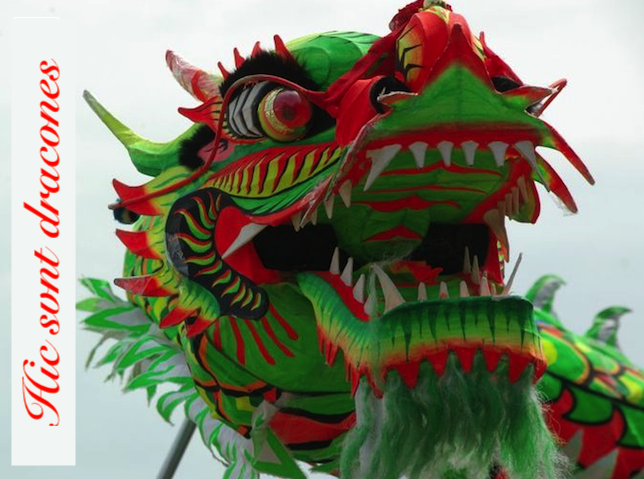
\includegraphics[width=0.75\textwidth]{imagenes/hic-svnt-dracones}
	\vspace{2cm}
	\begin{flushright}
		{\normalsize \textcolor{darkgray}{\textit{Ignacio Vallés Oriola}} \par}
	\end{flushright}
\end{titlepage}


\tableofcontents

\chapter*{}

%$ \ddot{x} \quad 	\displaystyle \dot{x} \quad  \va*{a} \quad \fdv{g} \quad \fdv{F}{g} \quad \fdv{V}(E-TS) \quad  \fdv*{F}{x}$

%\textsf{Este libro está enfocado a aquellos alumnos que van a emprender carreras científicas que necesitan de más contenidos matemáticos que los aprendidos en bachillerato, por tanto, se suponen conocidos todos los temas allí tratados, quien lea el libro debe saber manejarse con soltura ante sistemas de ecuaciones lineales, matrices y determinantes, conocer el producto escalar y vectorial de vectores y saber derivar e integrar con soltura.} 

%\textsf{Se mostrarán, de forma sencilla y con gran cantidad de ejercicios resueltos y propuestos con solución, algunos de los temas que se afrontarán en los primeros cursos de carrera. Para ello será necesario perder el rigor necesario en matemáticas pero será en pos de aclarar los conceptos, al cursar estudios universitarios recuperaréis el rigor que ahora, de momento, abandonamos. Espero que sea de utilidad.}


%Análisis (Funciones, límites, derivadas y cálculo de primitivas) $\longrightarrow$  mi libro %**********

%Estadística y Probabilidad (Cálculo probabilidades, Binomial y Normal, Correlación)  $\longrightarrow$  mi libro %*******

%PRECÁLCULO: aritmética, álgebra, trigonometría, complejos y geometría analítica (con cónicas).

\vspace{1cm}

\textbf{Estructura}

$\qquad$ 


\begin{cuadro-gris}
	
\end{cuadro-gris}

\begin{cuadro-naranja}
	
\end{cuadro-naranja}

\begin{destacado}
	
\end{destacado}

\begin{theorem}
	
\end{theorem}

\begin{definition}
	
\end{definition}

\begin{miejemplo}
	
\end{miejemplo}


\begin{miejercicio}
	
\end{miejercicio}

\begin{mipropuesto}
	
\end{mipropuesto}

\begin{myblock}{myblock}
	
\end{myblock}

\begin{myalertblock}{myalertblock}
	
\end{myalertblock}

\begin{myexampleblock}{myexampleblock}
	
\end{myexampleblock}




$\qquad$


$\qquad$



\emph{\normalsize{Este} documento se comparte bajo licencia `Creative Commons Attribution-NonCommercial-ShareAlike (4.0 CC BY-NC-SA)'}


\begin{multicols}{2}
\begin{figure}[H]
	\centering
	
\includegraphics[width=.5
	\textwidth]{imagenes/licencia.png}
\end{figure}
\begin{figure}[H]
	\centering
	
\includegraphics[width=.25
	\textwidth]{imagenes/firma.png}
\end{figure}
\end{multicols}

\newpage




\newpage

$\,$

\newpage

$\,$

\vspace{1cm} 

$\,$




\begin{center}

\Huge{\textbf{Precálculo}}

\huge{\textbf{---}} 


\Large{\textbf{\textit{Matemáticas primero de bachillerato}}}

\vspace{10mm}


\vspace{2cm}
\begin{flushright}
	\normalsize{\emph{Ignacio Vallés Oriola}}
\end{flushright}


\end{center}





 %Presentación
\part{Aritmética y Álgebra}


\null\vfill
\begin{Huge}\begin{center}
I. Aritmética y Álgebra
\end{center}\end{Huge}

\vspace{1.5cm}


\begin{figure}[H]
	\centering
	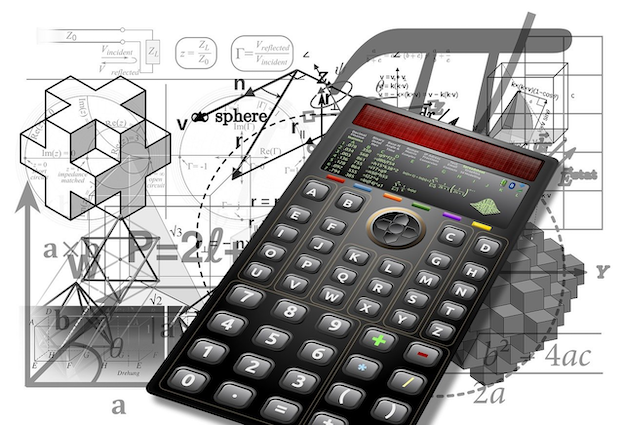
\includegraphics[width=.9\textwidth]{imagenes/part1.png}	
\end{figure}
\par
\vfill

\chapter{Números reales}
%\setlength{\parindent}{0cm}

\begin{tikzpicture}
	\fill [left color=red!50, right color=teal!50] (0,0) rectangle (6.5,.2);
	\fill [left color=teal!50, right color=blue!50] (6.5,0) rectangle (11.5,.2);
	\end{tikzpicture}

\vspace{15mm}


\begin{adjustwidth}{40pt}{40pt}
\begin{cuadro-gris}

	\begin{multicols}{2}
	$\triangleright \quad$  Intervalos, valor absoluto.
	
	$\triangleright \quad$  Radicales: racionalización.
	
	$\triangleright \quad$  Logaritmos.
	
	$\triangleright \quad$  Números combinatorios. Binomio de Newton.
	\end{multicols}
	
\end{cuadro-gris}
\end{adjustwidth}


\begin{figure}[H]
	\centering
	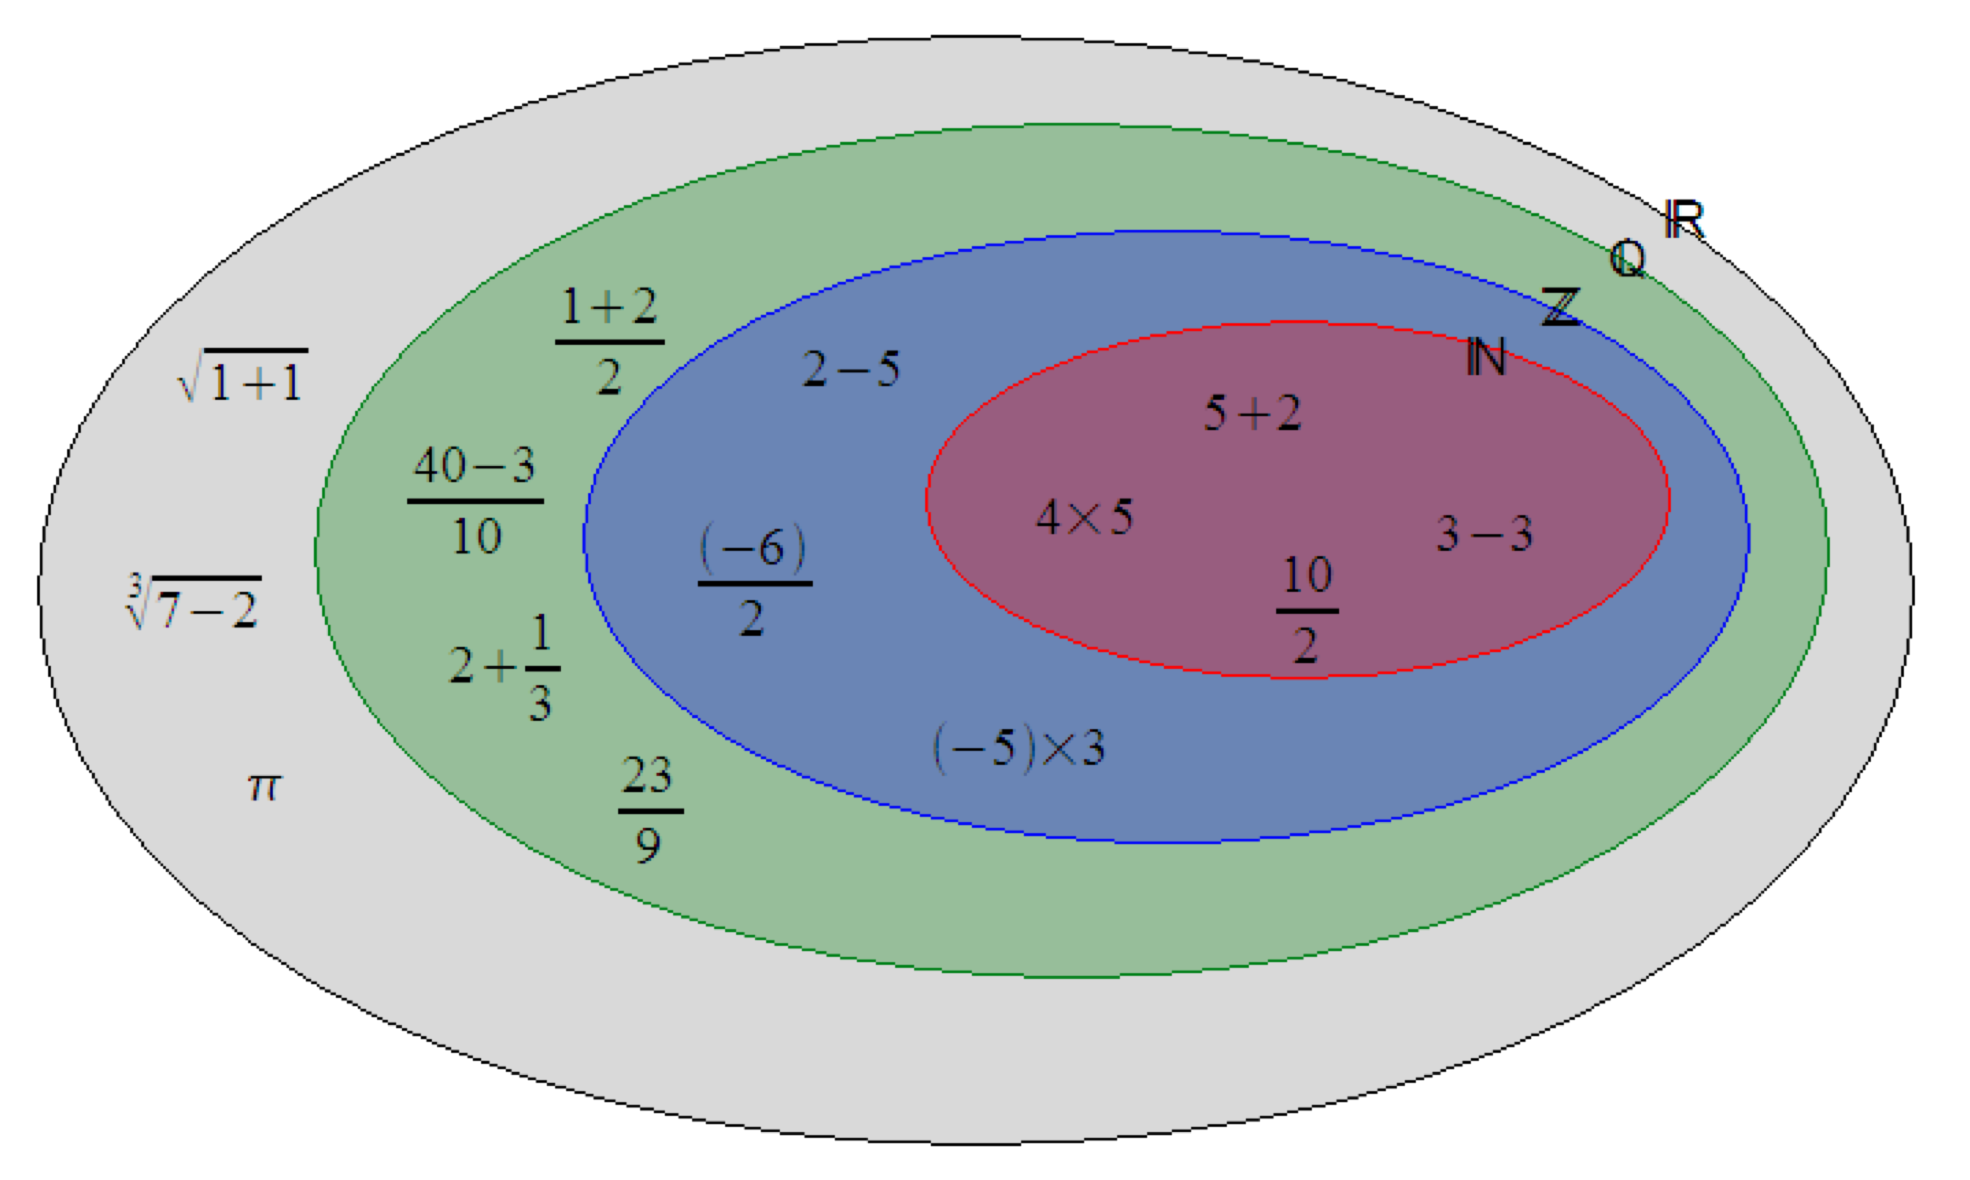
\includegraphics[width=.7\textwidth]{img-reales/reales00.png}	
\end{figure}


\section{Sucesivas ampliaciones de los conjuntos numéricos}
\begin{tikzpicture}
	\fill [left color=red!50, right color=teal!50] (0,0) rectangle (3.5,.1);
	\fill [left color=teal!50, right color=blue!50] (3.5,0) rectangle (7.5,.1);
	\end{tikzpicture}
\vspace{1cm}


Aunque la aparición de los distintos tipos de números no fue la que parecería lógica según sus relaciones de inclusión: primero los naturales, enteros, racionales hasta llegar a los reales;  permítaseme esta pequeña licencia narrativa a título meramente didáctico: \emph{``Y el hombre creó al número''}


\newpage %%%%%%%%%%%%%%%%%%%%%%%%%%%%%%%%%%

$\qquad$ %%%%%%%%%%%%%%%%%%%%%%%%%%%%%%%%%%

\begin{adjustwidth}{25pt}{25pt}

\begin{myexampleblock}{Y el hombre creó al número}
	
\vspace{3mm} 
\begin{multicols}{2}
Al principio, el ser humano sintió la necesidad de contar para, por ejemplo, saber la prole a la que tenía que alimentar (cuántas bocas tenía en la cueva). Estamos ante el nacimiento de los \emph{números naturales}, $\mathbb N$.
\begin{figure}[H]
	\centering
	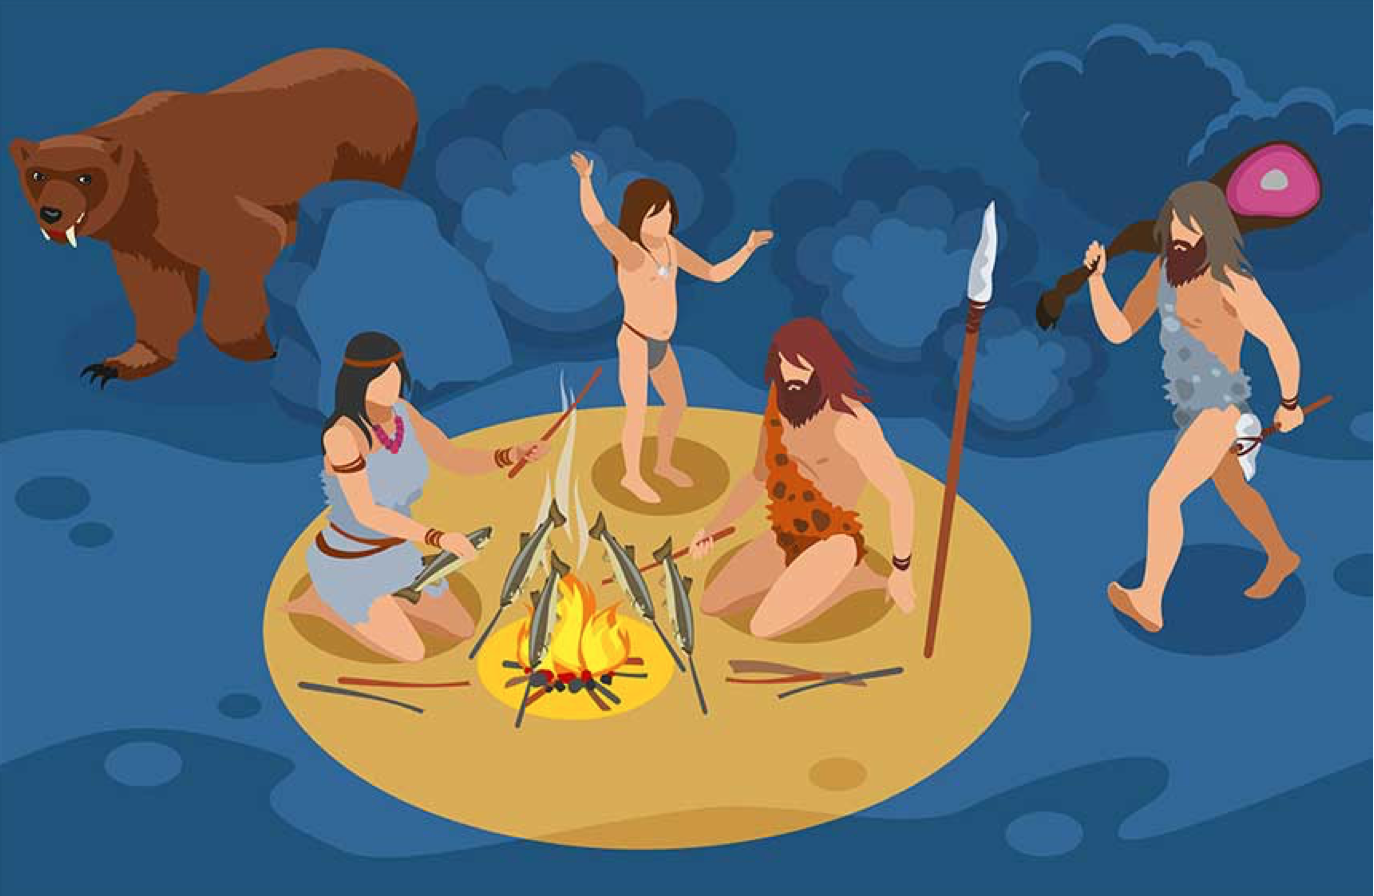
\includegraphics[width=.4\textwidth]{img-reales/reales01.png}	
\end{figure}
\end{multicols}

\vspace{3mm} 
\begin{multicols}{2}
\begin{figure}[H]
	\centering
	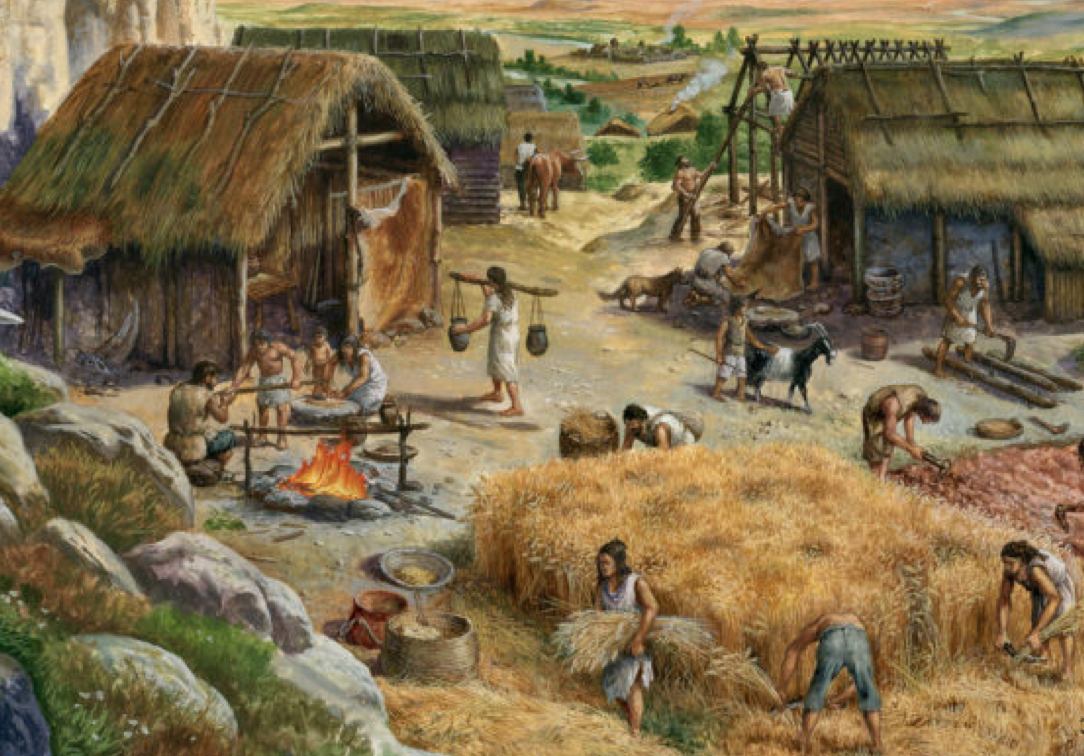
\includegraphics[width=.4\textwidth]{img-reales/reales02.png}	
\end{figure}
Pasó el tiempo y varios de ellos se juntaron en pequeñas tribus. Aparece el reparto del trabajo, lo que  conlleva la necesidad de restar: de la cantidad que te adeudo te pago esta cantidad, con lo que aún te debo esta otra. Surgen los \emph{números enteros}, $\mathbb Z$.
\end{multicols}	

\vspace{3mm} 
\begin{multicols}{2}
Las sociedades iban creciendo y aumentando sus temores a la oscuridad y a lo desconocido por lo que crean a sus primeras divinidades a las que adorar a cambio de protección y elevación de grandes templos. Tienen la necesidad de medir y ello lleva a dividir ampliando los números conocidos hasta entonces y aparecen los \emph{números racionales}, $\mathbb Q$.
\begin{figure}[H]
	\centering
	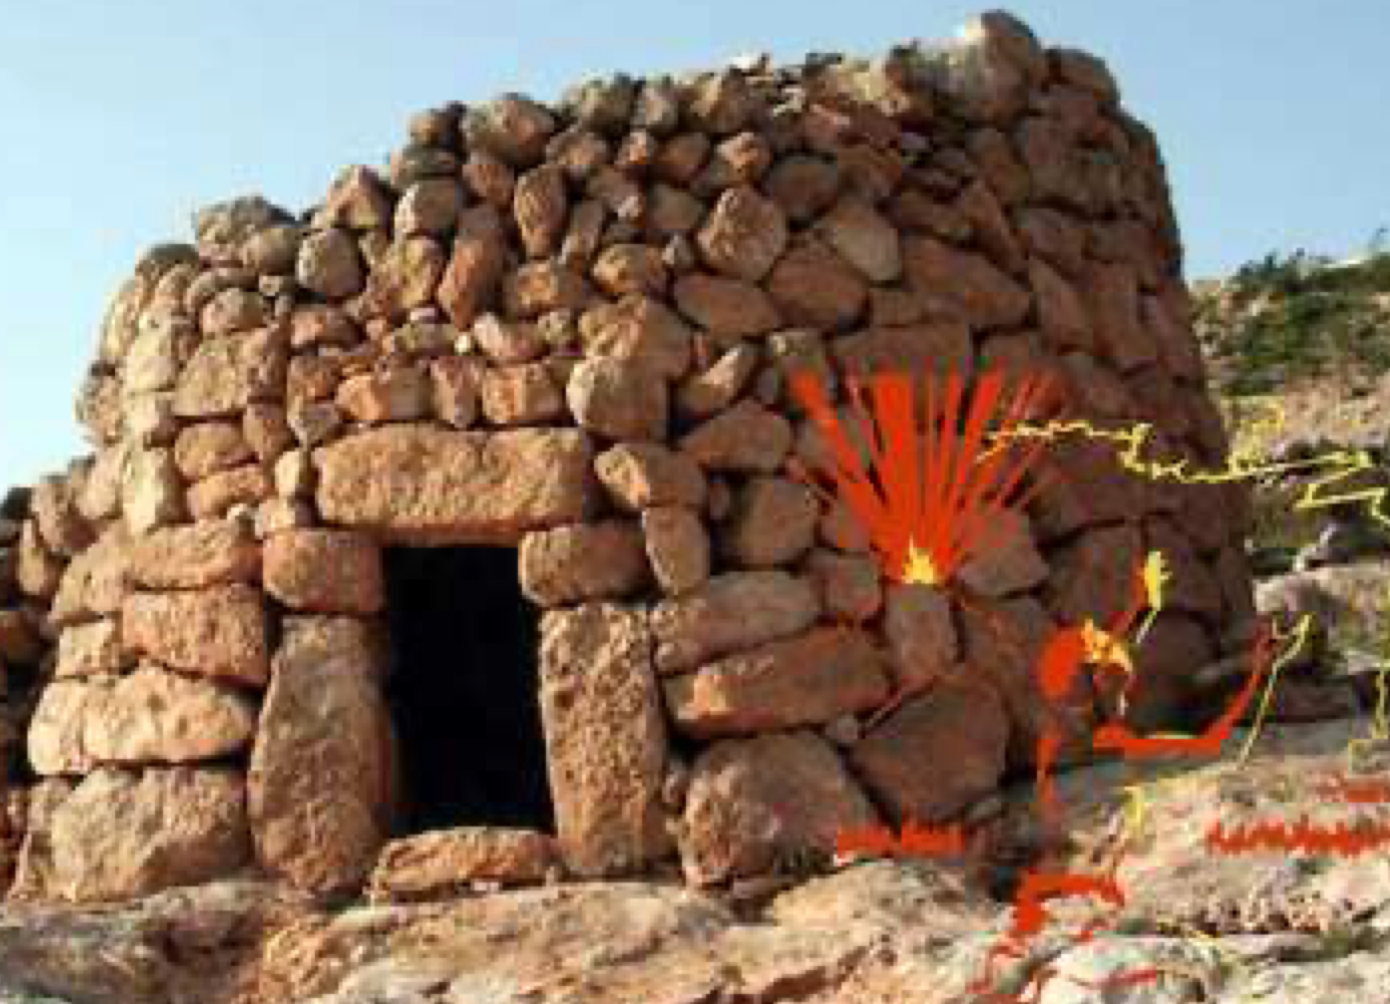
\includegraphics[width=.45\textwidth]{img-reales/reales03.png}	
\end{figure}
\end{multicols}

\vspace{3mm} 
\begin{multicols}{2}
\begin{figure}[H]
	\centering
	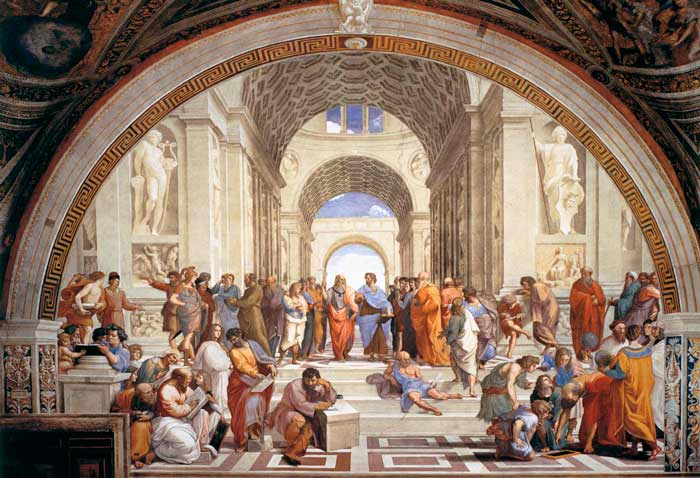
\includegraphics[width=.44\textwidth]{img-reales/reales04.png}	
\end{figure}
Profundizando en estos últimos números se dan cuenta de la existencia de otros verdaderamente extraños, no pueden tratarse como números racionales, son \emph{inconmensurables} (los llamados \emph{números irracionales}). La unión de ambos tipos de números dará lugar a los \textbf{\emph{números reales}}, $\boldsymbol{\mathbb R}$.
\end{multicols}

\end{myexampleblock}
\end{adjustwidth}

\newpage %%%%%%%%%%%%%%%%%%%%%%%%%%%%%%%%%%

\begin{multicols}{2}
En $\mathbb{N}$ podemos sumar y multiplicar, pero no restar ni dividir: $\ 2-5 \notin \mathbb{N}$ ($-3$ no es un número natural); $\ \frac 5 2 \notin \mathbb{N}$ ($\frac 5 2$ no es un número natural).

\begin{figure}[H]
	\centering
	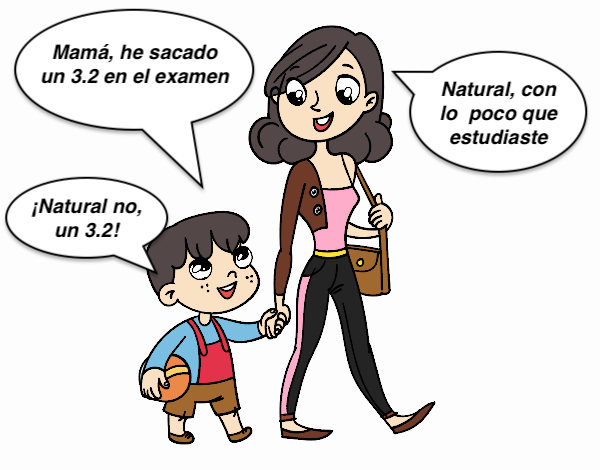
\includegraphics[width=.4\textwidth]{img-reales/reales05.png}	
\end{figure}

Este inconveniente se resuelve con los número enteros, $\mathbb{Z}$, ahora la resta no tiene ningún problema, $-3 \in \mathbb{Z}$ ($-3$ es un número entero). Continuamos, eso sí, sin poder dividir: $\frac 6 2 $ tiene sentido, da $3$, pero $\frac 2 6$ no lo tiene, no es un número entero.



Los números racionales, $\mathbb{Q}$, son la solución al problema, cualquier pareja de enteros que queramos dividir es posible, el resultado es siempre un número racional. Con números racionales ya podemos realizar las cuatro operaciones básicas: suma, resta, multiplicación y división (salvo, claro está, dividir por cero; esa operación no está definida).

Es sabido que la expresión decimal de cualquier número racional da como resultado un número periódico, pero no es difícil encontrar números decimales no periódicos: $0.101001000100001\cdots$ que no se pueden expresar como fracción (números racionales). Son los números irracionales los que, junto con los racionales, completan el conjunto de los números reales.
\end{multicols}

\begin{multicols}{2}
$$ \subrayado{ \mathbb N \subset \mathbb Z \subset \mathbb Q \subset \mathbb R }$$ 

$$\subrayado{ \mathbb R \supset \mathbb Q \supset \mathbb Z \supset \mathbb N }$$ 
\end{multicols}

$ \mathbb N=\{1,2,\cdots,817,\cdots \} \subset \mathbb Z \, ; \quad \mathbb Z=\{\cdots,-2,-1,\boldsymbol{0},1,2,3,\cdots \} \supset \mathbb N$

$ \mathbb Q=\left\{  \dfrac p q  \, / \,  p,q \in \mathbb Z \, , \ q>0  \ \wedge  \textcolor{gris}{(\text{y})} \ \   mcd ( |p|  ,q )=1  \right\}   \supset Z  \supset  N = \{\text{ fracciones  decimales periódicos } \}$
  
$\mathbb Q$ es \emph{denso}: entre dos racionales cualesquiera siempre se puede encontrar otro número racional (por ejemplo,  su media aritmética). No obstante, en la recta numérica (\emph{recta real}) hay infinitos puntos no ocupados por números racionales (decimales no periódicos, que no se pueden escribir como fracción).  A cada uno de estos puntos le corresponde un número irracional.  Ejemplos de número irracionales son  $\  0.1234\cdots \, ; \   1.010010001\cdots \, ; \ \sqrt{2}\, ; \ \pi \, ; \cdots$   

Los números irracionales se caracterizan porque: 
$\ a) \ $no pueden expresarse en forma de fracción, $\ b)\ $ su expresión decimal tiene infinitas cifras no periódicas. 

El conjunto de todos los números irracionales se designa por $\mathbb Q \smallsetminus \mathbb R$. 

\begin{adjustwidth}{25pt}{0pt}
$\triangleright\ \ $ Si $p$ no es cuadrado perfecto, $\sqrt{p}$ es irracional: $\sqrt{7}$ es irracional.

$\triangleright\ \ $ En general, cualquier raíz enésima no exacta es irracional: $\sqrt[5]{31}$ es irracional.

$\triangleright\ \ $ La operación de un número racional con uno irracional da un resultado irracional (excepto la multiplicación por cero): $3\cdot \sqrt{2}-4$ es irracional.

$\triangleright\ \ $ Irracionales famosos:  $\pi,\, \phi, \, e,\, \cdots$
\end{adjustwidth}

La unión de los números racionales y los irracionales forman los números reales. El conjunto de los números reales se designa por $\mathbb R$. \emph{Los números reales llenan la recta numérica por eso se la llama recta real}.  $\ \mathbb R$ es completo: a cada punto de la recta le corresponde un  único número real y cada número real se representa por un único punto en la recta (correspondencia biunívoca).

$$\boxed{ \ \boldsymbol{ \subrayado{\mathbb N \subset \mathbb Z \subset \mathbb Q \subset \mathbb R} } \ }$$

$$\text{Números Reales }
\begin{cases}
\ \text{ Racionales } 
	\begin{cases}
	\text{ Enteros } 
		\begin{cases}
		\text{ Naturales } \, : 1,\, 2,\, 	\cdots ,\, 139,\ \cdots \\
		\text{ No positivos }\, : \ -17,\,  0,\, \cdots
		\end{cases}
	\\
	\text{ Fraciones } \, : \ \dfrac 2 3,\, 7.0\widehat{34},\, \cdots
	\end{cases}	
\\
\ \text{ Irracionales }\, : \ \sqrt{2},\ \sqrt[3]{5},\ \pi,\ \cdots 
\end{cases}$$


\vspace{5mm}

\begin{myexampleblock}{ $\sqrt{2}$ es irracional.\hspace{5mm} \emph{Demostración por reducción al absurdo}}


\color{teal}\rule{250pt}{0.1pt}

\begin{footnotesize}{\textcolor{teal}{La `demostración por reducción al absurdo' es uno de los métodos de demostración más usados en matemáticas. Se parte por suponer como hipótesis la falsedad de lo que se quiere demostrar y, mediante una concatenación de inferencias lógicas, se pretende llegar a una contradicción, un absurdo. Al llegar a una contradicción, se concluye que la hipótesis de partida (que se había supuesto falsa al principio) ha de ser verdadera.}}\end{footnotesize}
\vspace{-5mm}
\begin{flushright}
\color{teal}\rule{250pt}{0.1pt}	
\end{flushright}
 
\color{black}

\normalsize{Supongamos} que $\sqrt{2}$ no fuese un número irracional, que fuese racional. Acabaremos llegando a una contradicción por lo que podremos concluir que, necesariamente, $\sqrt{2}$ es irracional.

\vspace{2mm} Si $\sqrt{2}$ es racional, deberán existir dos enteros $p,\, q \in \mathbb Z$, de modo que podamos escribirlo como una fracción:
$\ \sqrt 2=\dfrac p q\, , \ $ siendo $p \text{ y } q$ primos entre sí (co-primos) para que la fracción sea irreducible.

\vspace{2mm} Elevando al cuadrado, $\ 2=\dfrac {p^2}{q^2} \ \Rightarrow \ 2q^2=p^2\, \ $ de lo que deducimos que $p^2$ ha de ser par, múltiplo de $2$ y, necesariamente, también lo será $p$. Podremos escribir $p=2k$, para algún $k\in \mathbb Z$

\vspace{2mm} Sustituyendo en la expresión anterior, $ 2=\dfrac{(2k)^2}{q^2}=\dfrac{4k^2}{q^2} \ \Rightarrow \  q^2=2k^2\ $ y obtenemos que $q^2$ también es par, así como también lo será $q=2l$, para algún $l \in \mathbb Z$.

\vspace{2mm} Podremos escribir $\ \sqrt{2}=\dfrac p q = \dfrac{\cancel{2} k}{\cancel{2} l}=\dfrac k l \ $ lo que entra en contradicción con la hipótesis de partida, que $\dfrac p q$ era fracción irreducible.

\vspace{2mm} Conclusión: $º \sqrt{2}$ es \emph{irracional} \footnote{ $\ \ $ El símbolo $\blacksquare$  es típico al final de las demostraciones en matemáticas y significa \emph{``quod erat demostrandum'', `como queríamos demostrar'}, indica que la demostración ha acabado} \QED
 
\vspace{5mm}
	
\end{myexampleblock}

\vspace{5mm}
\color{teal}
\rule{250pt}{0.1pt}	

?`Cuántos números hay?. En realidad la cantidad de números naturales es infinita, pero hay infinitos más grandes que otros. Al infinito de los números naturales se le llama \emph{infinito numerable} y se puede demostrar que en los números enteros y los racionales hay también un infinito numerable de ellos. Pero números irracionales (y por lo tanto reales) hay más, ya no forman un infinito numerable y se le llama \emph{potencia del continuo}.
\vspace{-5mm}
\begin{flushright}
\rule{250pt}{0.1pt}	
\end{flushright}
\color{black}
\vspace{5mm}

\begin{miejercicio}

Clasifica los siguientes números según el menor conjunto numérico al que pertenezcan:

\begin{table}[H]
\centering
\begin{tabular}{|c|c|c|c|c|c|c|c|}
\hline
$\quad \sqrt{3} \quad$ & $\quad 5 \quad$  & $\quad -2 \quad$ & $\quad 4.5 \quad$ & $\quad 7.\widehat 3 \quad$ & $\quad -\sqrt[3]{6} \quad$ & $\quad \sqrt{64} \quad$ & $\quad \sqrt[3]{-27} \quad$  \\ \hline \hline
$\mathbb{R}$ & $\mathbb{N}$ & $\mathbb{Z}$ & $\mathbb{Q}$ & $\mathbb{Q}$ & $\mathbb{R}$ & $\mathbb{N}$ & $\mathbb{Z}$     \\ \hline
\end{tabular}
\end{table}
\end{miejercicio}

\begin{miejercicio}

Da tres números racionales y tres irracionales comprendidos entre $5.1112\cdots$ y $5.1222....$

\rule{250pt}{0.1pt}

\vspace{3mm}
$\mqty{
\ \bold{5.11}12\cdots \\
\ \bold{5.12}22\cdots 
} \ \to \ 5.11X \ (X>1)\ \to \ $ Problema abierto, por ejemplo,

$\to \ 
\begin{cases}
\text{ racionales: }	\ & 5.115; \ 5.1155;\, 5.115\widehat 3 
\\
\text{ irracionales: } \ & 5.1151234\cdots;\ 5.115101001000\cdots;\ 5.115101101110\cdots
\end{cases}
$
 	
\end{miejercicio}


%%%%%%%%%%%%%%%%%%%%%%%%%%%%%%%%%%%%%%%%%%%%%%%%%%%%%%%%%%%%%%%%%%%%%%%%%%%%%%%%%%%%%%%%%%%%%%%%%%%%%%%%%%%%%%%%%%%%%%%%%%%%%%%%%%%%%%%%%%
\vspace{10mm}
\subsection{Valor absoluto}
\begin{tikzpicture}
	\fill [left color=red!50, right color=teal!50] (0,0) rectangle (3.5,.01);
	\fill [left color=teal!50, right color=blue!50] (3.5,0) rectangle (7.5,.01);
	\end{tikzpicture}
\vspace{0.5cm}
	
	\begin{definition}[ Valor Absoluto] 
	
	El valor absoluto de un número real $\, x\in \mathbb R\, $ se define como el número:
	\begin{multicols}{2}
	$\quad$
	
	\begin{equation*}
		|x|=
		\begin{cases} 
		\;\;  x &\mbox{ si } x\ge 0 \\ 
		\; -x & \mbox{ si } x<0 
		\end{cases}
	\end{equation*}	
	
	$\quad$
	\begin{figure}[H]
	\centering
	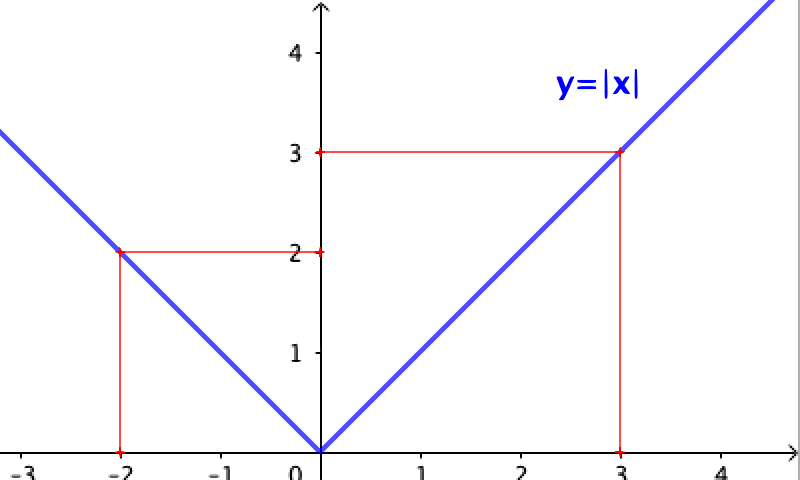
\includegraphics[width=.3\textwidth]{img-reales/reales06.png}	
\end{figure}
	\end{multicols}
	\end{definition}

El valor absoluto es, en matemáticas el \textit{gran positivizador}: $\ |3|=3;\ \ |-2|=-(-2)=2; \ \ |0|=0$.
	
%%%%%%%%%%%%%%%%%%%%%%%%%%%%%%%%%%%%%%%%%%%%%%
 
 Obsérvese que para eliminar las barras del valor absoluto nos tenemos que fijar en el signo de lo que vaya dentro de las barras del valor absoluto. Si es positivo queda igual y si es negativo, cambiamos el signo de lo que vaya dentro.

 El problema se nos presenta cuando no conozcamos el signo. Por ejemplo, resolver la siguiente ecuación con valor absoluto $|x|=3$.
 
Para resolverla, lo primero es quitar el valor absoluto. Debemos conocer el signo de lo de dentro, de $x$. Como no lo sabemos, no podemos quitar el valor absoluto. En estos casos se supone que lo de dentro del valor absoluto puede presentar los dos signos, luego el problema tiene doble solución:

$\begin{cases}
\text{ si } x>0 \ (\text{positivo})\ \to |x|=x=3  & \Rightarrow \boldsymbol{x=3}
\\ 
\text{ si } x<0 \, (\text{negativo})\, \to |x|=-x=3  & \Rightarrow \boldsymbol{x=-3}
\end{cases} \qquad  \boldsymbol{ |x|= 3 \ \Leftrightarrow \ x=3 \, \vee \textcolor{gris}{(\text{o})} \ x=-3 }$

\vspace{5mm}
\begin{miejercicio}

Resuelve la ecuación: $\qquad \left| \dfrac{2x-3}{4} \right| = 5$	

\vspace{2mm}
\rule{250pt}{0.1pt}
\vspace{2mm}

$\left| \dfrac{2x-3}{4} \right| = 5 \Leftrightarrow \begin{cases}
\ \dfrac{2x-3}{4} = 5 \to \ \ 2x-3=\ 5\cdot 4\ \to 2x=\ 23 & \Rightarrow \boldsymbol{x=23/2}
\\
\ \dfrac{2x-3}{4} = -5 \to  2x-3=-5\cdot 4\to 2x=-17 & \Rightarrow \boldsymbol{x=-17/2}
 \end{cases}$


\end{miejercicio}


\vspace{5mm}
\begin{theorem}[ Propiedades del valor absoluto] 	
	
	\begin{enumerate}
		\item $\quad  |-x|=|x|$
		\item $\quad |xy|=|x|\cdot|y|$
		\item $\quad \left| \dfrac x y \right| = \dfrac {|x|}{|y|}$
		\item $\quad |x|\le y\;  \mbox{ es equivalente a } -y\le x \le y $
		\item $\quad |x+y|\le|x|+|y|\qquad$ \emph{Desigualdad Triangular}
	\end{enumerate}
\end{theorem}	

\begin{multicols}{2}
Es sencillo comprobar con ejemplos que las afirmaciones anteriores son ciertas, las demostraciones rigurosas se dejan para cursos superiores. 

Una figura como demostración sin palabras de la desigualdad triangular. Se entiende por $|\vec a|$ al módulo (tamaño) del vector (segmento orientado) $\vec a$.
	
\begin{figure}[H]
	\centering
	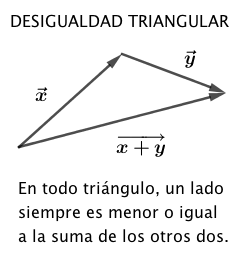
\includegraphics[width=0.3\textwidth]{img-reales/reales07.png}
\end{figure}
\end{multicols}

		
\begin{definition} [ Distancia entre números reales]

Llamamos \emph{distancia} $d$ entre dos números $x,y:\quad$ $ d(x,y)=|y-x|\, , \quad \forall x,y \in \mathbb R \ $ \footnote{ El símbolo $\ \forall \ $  se lee \emph{`para todo'}: $\ \forall x,y\in \mathbb R$ significa `para todo $x$ e $y$ números reales', es decir, para $x$ e $y$ dos números reales cualesquiera.}
\end{definition}
		


\begin{theorem}[ Propiedades de la distancia]

Se cumplen las siguientes propiedades para las distancias ($\forall$ se lee `para todo'). 
		
\begin{enumerate}[D1]
	\item  $\qquad \forall x \in \mathbb R:\; \ \ d(x,x)=0 $
	\item  $\qquad \forall x, y \in \mathbb R:\; \ \ d(x,y)=d(y,x)$
	\item  $\qquad \forall x, y, z \in \mathbb R:\; \ \ d(x,z) \le d(x,y)+d(y,z)$
\end{enumerate}
\end{theorem}		
		
\underline{Demostración}: En este caso, por su sencillez, demostramos el teorema para que el lector/a vaya acostumbrándose a ellas.

$\triangleright \ D1:\quad d(x,x)=|x-x|=|0|=0$ \QED

$\triangleright \ D2:\quad d(x,y)=|y-x| \mqty{ * \\ \leq \\ \ } |-(y-x)|=|x-y|=d(y,x)$ \QED

$*\ $ Hemos usado la propiedad $1.\, $ del valor absoluto, $|z|=|-z|$. 

$\triangleright \ D2:\quad d(x,z)=|z-x|=|z-y+y-x|\mqty{ ** \\ \leq \\ \ }|z-y|+|y-x|=d(y,z)+d(x,y)$ \QED

$**\ $ En la última demostración hemos usado la `desigualdad triangular'. 

Los símbolos $\blacksquare$ significan que la demostración ha acabado y se leen \emph{`como queríamos demostrar'} (quod erat demonstrandum, en latín). En textos antiguos aparece como siglas, \emph{q.e.d.}

\vspace{5mm}
\subsection{Intervalos}
\begin{tikzpicture}
	\fill [left color=red!50, right color=teal!50] (0,0) rectangle (3.5,.01);
	\fill [left color=teal!50, right color=blue!50] (3.5,0) rectangle (7.5,.01);
	\end{tikzpicture}
\vspace{.5cm} %%%%%%%%%%%%%%%%%%%%%%%
		
	
\begin{definition}[ Intervalos] 
	
Un intervalo es un subconjunto $I \subset \mathbb R$ tal que $\forall u,w \in I\; $, con $u\neq w\; $, y $\forall v \in \mathbb R\; $ con $u<v<w\; $ se cumpla que $v\in I$. Los intervalos pueden ser abiertos, cerrados y semiabiertos.\end{definition}

Esta es la definición rigurosa, necesaria en matemáticas, pero lo podemos entender como un subconjunto de números reales que se encuentran entre dos valores que delimitan un extremo inferior y otro superior. Los intervalos pueden ser abiertos o cerrados en cada uno de sus extremos, incluso pueden ser no acotados.

$\forall a,b \in \mathbb R\, ,\ $ se definen:
	
		\begin{figure}[H]
			\centering
			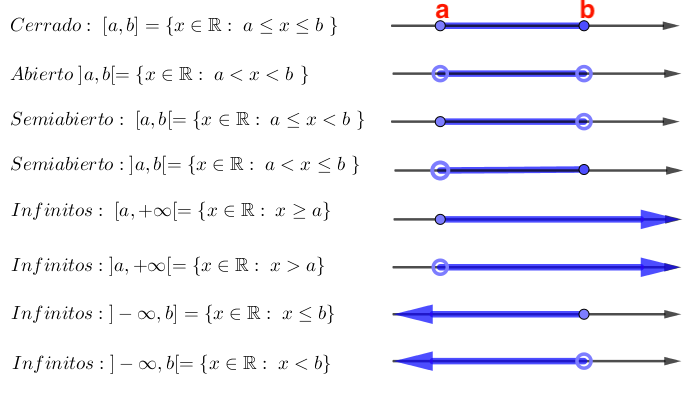
\includegraphics[width=0.8\textwidth]{img-reales/reales08.png}
		\end{figure}

\begin{miejercicio}

Da como notación de intervalos los siguientes subconjuntos de $\mathbb R$:

$a)\ \{ x\in \mathbb R \, / \, -2\leq x < 3 \} $ \footnotesize{(número reales tales que estén comprendidos entre -2 -inclusive- y 3 -exclusive-)} \normalsize{;} $\ \ b)\ \ $ número mayores que $-1$.

\vspace{3mm} \rule{250pt}{0.1pt}
\vspace{3mm}

Basta con representar los conjuntos en la recta real para determinar los intervalos buscados. Hemos tomado por convenio el dibujar un punto relleno para representar las igualdades ($\leq,\ \geq$) y un punto vacío para las desigualdades estrictas ($<,\ >$).

\begin{figure}[H]
			\centering
			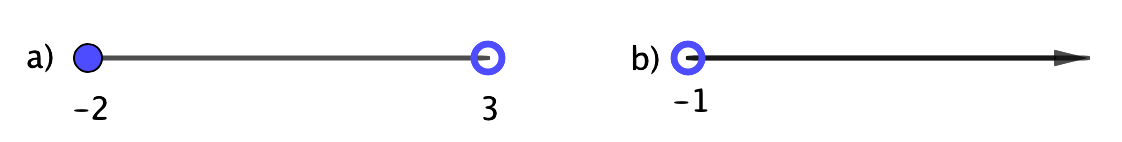
\includegraphics[width=0.7\textwidth]{img-reales/reales10.png}
		\end{figure}
		
Solución: $\quad a)\ \ [-2,3[\, ; \qquad b)\ \ ]-1,\infty]$
\end{miejercicio}

\vspace{5mm}


\begin{miejercicio}

Calcula :  $\qquad a) \ \ [1,4] \, \cup \, ]2,5[\, ; \qquad \qquad b)\ \ [1,4] \, \cap \, ]2,5[	$

\vspace{3mm}
\rule{250pt}{0.1pt}
\vspace{3mm}

Basta con representar los intervalos en la recta real, uno de ellos lo rayamos en vertical y el otro en horizontal. La unión $(\cup)$ será toda la zona rayada y la intersección $(\cap)$
 la zona con ambas rayas (zona cruzada).
 
 \begin{multicols}{2}
\begin{figure}[H]
			\centering
			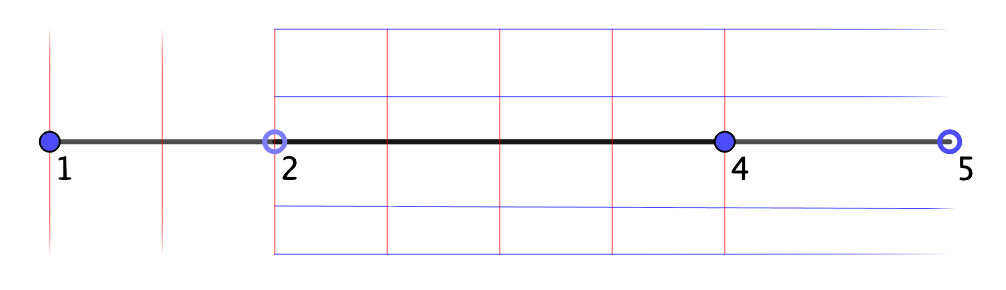
\includegraphics[width=0.45\textwidth]{img-reales/reales11.png}
		\end{figure} 	
		$\qquad \qquad a) \quad [1,5[$
		
		$\quad$
		
		$\qquad \qquad b) \quad ]2,4]$
 \end{multicols}

 
 \end{miejercicio}
	
\vspace{1cm}		
\begin{definition}[ Entorno]: 
	
$\forall a \in \mathbb R, \; \forall r \in \mathbb R^{+} \ $\footnote{ $\ \mathbb R^+\, \equiv ]0,+\infty[\, , $ son los números positivos. }
se define el \emph{entorno} de centro $a$ y radio $r$ como todos los números reales cuya distancia a $a$ sea menor que $r$:

$$\quad E_r(a)=\{ \forall x \in \mathbb R \;  / \; d(x,a)<r \}=]a-r,a+r[$$
		
\vspace{3mm} Se define el \emph{entorno reducido} de centro $a$ y radio $r$ como todos los números reales cuya distancia a $a$ sea menor que $r$, excluyendo al número $a$:
		
$$\quad E^*_r(a)=\{ \forall x \in \mathbb R \;  / \; 0<d(x,a)<r \}=]a-r,a+r[\smallsetminus \{a\} \small{\textcolor{gris}{\ = ]a-r,a[\cup ]a,a+r[}}$$
			
\end{definition}

\vspace{4mm} 

	
	\begin{myalertblock} {Valores Absolutos e Intervalos.}
		\begin{multicols}{2}
		\begin{itemize}
			\item $|x|=k \longleftrightarrow x=\pm k$
			\item $|x|<k \longleftrightarrow -k<x<k \longleftrightarrow ]-k,k[$
			\item $|x|\le k \longleftrightarrow -k\le x\le k \longleftrightarrow [-k,k]$
			\item $|x|> k \longleftrightarrow x>k\quad o \quad x<-k$
			\item $|x|\ge  k \longleftrightarrow x\ge k\quad o \quad x\le -k$
		\end{itemize}
		\begin{figure}[H]
			\centering
			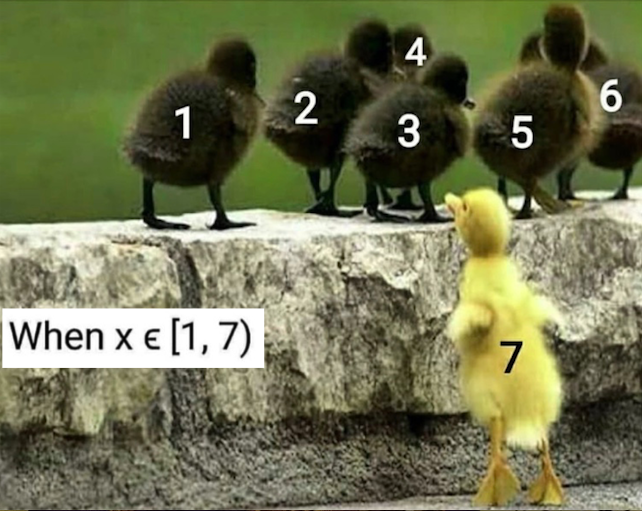
\includegraphics[width=0.4\textwidth]{img-reales/reales09.png}
		\end{figure}
		\end{multicols}
	\end{myalertblock}
		
\vspace{4mm} \underline{Nótese que}:  \hspace{.5cm} en el intervalo $[2,5[$, $2 \in [2,5[$, sin embargo, $5 \notin [2,5[$.

\vspace{4mm}\underline{Nota}: \hspace{.5cm} En muchos textos, los intervalos abiertos aparecen con paréntesis en lugar de corchetes, $]a,b[\equiv (a,b);\ [c,d[\equiv [c,d)\, . $ Nosotros continuaremos utilizando los corchetes para evitar la posible confusión con la notación para las coordenadas cartesianas de puntos en el plano.

\vspace{1cm}
\section{Radicales}
\begin{tikzpicture}
	\fill [left color=red!50, right color=teal!50] (0,0) rectangle (3.5,.1);
	\fill [left color=teal!50, right color=blue!50] (3.5,0) rectangle (7.5,.1);
	\end{tikzpicture}
\vspace{0.5cm}

\begin{definition}[ Radical ]

Se llama \emph{raíz $n$-sima} de un número real $a$, que representamos por $\sqrt[n]{a}$, al número real $b$ tal que $b$ sea la potencia $n$-sima de $a$:

$$ \boxed{ \ \boldsymbol{\sqrt[n]{a}\ = \ b \ \leftrightarrow \ b^n\ = \ a } \ }\qquad a,b\in \mathbb R,\quad n\in \mathbb N,\ n>1 $$

$\sqrt[n]{a}\,:\ $ radical; $\qquad a \, : \ $ radicando; $\qquad n\,: \ $ índice de la raíz	
\end{definition}

Si no aparece $n$ explícitamente se supondrá que es un $2$: raíces cuadradas.

\vspace{5mm} Dado un número real $a$ cualquiera y un natural mayor que uno, $n$, cualquiera, la ecuación $\ x^n=a\, $ tiene:

\vspace{-2mm}  \begin{itemize}
\vspace{-2mm} \item Dos soluciones, $+\sqrt[n]{a}$	 y $-\sqrt[n]{a}$ si $n$ es par y $a$ positivo.  
\vspace{-2mm} \item Las raíces pares de números negativos no existen.
\vspace{-2mm} \item Una solución única si $n$ es impar, siendo ésta positiva si lo es $a$ y negativa en caso contrario. 
\end{itemize}

$\sqrt[4]{16}=2;\ \ -\sqrt{25}=-5 ; \ \ \nexists \sqrt[4]{-1}; \ \ \sqrt[3]{-8}=-2; \ \ \sqrt[5]{1}=1 \qquad $ \textcolor{gris}{$\nexists$ se lee  \emph{`no existe'}}.

\vspace{5mm}
\begin{myalertblock}{Ambigüedad en el signo de la raíz cuadrada.}

Se considera que $\sqrt{x},\ x>0$ tiene solo un signo válido, el positivo. Así, escribiremos $\sqrt{4}=2;\ -\sqrt{4}=-2$

\vspace{2mm} Al resolver ecuaciones del tipo $(x+3)^2=16$,

\vspace{2mm} 
\begin{small}
$\begin{cases}
\text{ mal procedimiento: } \ & \\
\ (x+3)^2=169 \ \to \ \sqrt{(x+3)^2}=\sqrt{169} \ \to \ x+3=\pm 13 \ \to \ \begin{cases} \ x=10 \\ \ x=-16 \end{cases}
\\
\text{ procedimiento correcto: } \ & \\
\ (x+3)^2=169 \ \to \ \sqrt{(x+3)^2}=\sqrt{169} \ \to \ |x+3|=13 \ \to \ x+3=\pm 13  \ \to \ \begin{cases} \ x=10 \\ \ x=-16 \end{cases}
\end{cases}$
\end{small}
	
\end{myalertblock}



\vspace{5mm}\begin{definition}[ Potencias de exponente racional]

\begin{large}
$$\boldsymbol{ \sqrt[n]{a} \ = \ a^{\frac 1 n} \quad \longrightarrow \quad \sqrt[n]{a^m}\ = \ a^{\frac m n} } \qquad \qquad (\sqrt[n]{a})^m=\sqrt[n]{a^m} \ \ ( \circledast )$$	\end{large} 

\normalsize{Las} potencias de exponentes racionales son radicales siendo la base el radicando, el denominador del exponente de la potencia el índice de la raíz, el numerador el exponente del radicando.
\end{definition}

\textcolor{gris}{Justificación: $\qquad a^{1/n}=b \ \to \ (a^{1/n})^n=a=b^n \ \to \ b=\sqrt[n]{a}=a^{1/n}$}

$ \circledast \ $ En realidad, esta propiedad solo es cierta si existe $\sqrt[n]{a}$ y también $\sqrt[n]{a^m}$. Por ejemplo, $\ (\sqrt{-1})^2 \neq \sqrt{(-1)^2}$, la primera expresión no existe.

\vspace{5mm}\begin{miejemplo}

$\qquad 125^{\frac 1 3 }= \sqrt[3]{125}=5; \qquad \qquad 16^{\frac 3 4}=\sqrt[4]{16^3}=(\sqrt[4]{16})^3=2^3=8;$

$\qquad -9^{\frac 1 2}=-\sqrt{9}=-3; \qquad \qquad 	(-9)^{\frac 1 2}=\sqrt{-9}:\, \nexists$
\end{miejemplo}


\vspace{5mm}

\subsection{Propiedades de los radicales}
\begin{tikzpicture}
	\fill [left color=red!50, right color=teal!50] (0,0) rectangle (3.5,.01);
	\fill [left color=teal!50, right color=blue!50] (3.5,0) rectangle (7.5,.01);
	\end{tikzpicture}
\vspace{0.5cm}

\begin{theorem}[ Propiedades de los radicales. $\circledast$]
	
	\begin{enumerate}[P1. ]
	\item Suma: solo se pueden sumar radicales semejantes.
	
	$\sqrt[n]{a}+\sqrt[n]{b}=\sqrt[n]{a}+\sqrt[n]{b}; \qquad \qquad \sqrt[n]{a}+\sqrt[n]{a}=2\sqrt[n]{a}$	
	\item Producto: el producto de dos radicales del mismo índice es un radical de ese índice y radicando el producto de los radicandos factores.
	$ \ \ \boldsymbol{ \sqrt[n]{a}\cdot \sqrt[n]{b}=\sqrt[n]{a \cdot b}}$
	\item Cociente: para dividir dos radicales del mismo índice, se deja el mismo índice y se dividen los radicandos.
	$ \ \ \boldsymbol{ \dfrac{\sqrt[n]{a}}{\sqrt[n]{b}}=\sqrt[n]{\dfrac a b} }$
	\item Potencia: para elevar un radical a una potencia, se eleva el radicando y se deja la misma raíz. $\ \ \boldsymbol{(\sqrt[n]{a})^m = \sqrt[n]{a^m}}$
	\item Radicación: la raíz de otra raíz es la raíz del radicando e índice el producto de las raíces.  $\ \ \boldsymbol{ \sqrt[n]{\sqrt[m]{a}}=\sqrt[n\cdot m]{a} }$
	\end{enumerate}

\end{theorem}

$ \circledast \ $ Hay que tener en cuenta que estas propiedades son ciertas si existe todos los radicales que interviene en ellas. Por ejemplo, $\ (\sqrt{-1}) \cdot (\sqrt{-1}) \neq \sqrt{(-1)(-1)}=\sqrt{1}=1$, las primeras expresiones no existen.

\begin{miejemplo}

$\qquad \sqrt{2}-3\sqrt{2}+5\sqrt{2}=3\sqrt{2};\qquad \sqrt[3]{4}\, \sqrt[3]{8}=\sqrt[3]{32};\qquad \qquad \dfrac{\sqrt[5]{9}}{\sqrt[5]{16}}=\sqrt[5]{\dfrac{9}{16}};	$

$\qquad (\sqrt[3]{2})^5=\sqrt[3]{2^5} ; \qquad \qquad \qquad \sqrt[3]{\sqrt[4]{5}}=\sqrt[12]{5}$
\end{miejemplo}


\vspace{5mm} \begin{definition}[ Radicales equivalentes]
 
 	Dos radicales son equivalentes si dan el mismo resultado.
 	
$$3=\sqrt{9}\ =\ \sqrt[3]{27}\ = \ \sqrt[4]{81}\ = \ \sqrt[5]{3^5}\ = \ \cdots $$
 	
\vspace{2mm} 	Usando la notación de potencia de exponente racional,
 	
 	$$\boldsymbol{ \sqrt[n]{a^m}} \ =a^{m/n}=a^{m\cdot k/n\cdot k}= \boldsymbol{ \sqrt[nk]{a^{mk}}} $$
 	
\vspace{2mm} Leída esta propiedad de izquierda a derecha la podríamos llamar \emph{propiedad simplificativa} y se usará, por ejemplo, para sumar radicales semejantes. 
 
\vspace{2mm} Leída de derecha a izquierda la prodríamos llamar \emph{reducción a índice común} y la usaremos, por ejemplo, para multiplicar y dividir radicales de distinto índice, reduciéndolos a índice común (el mcm de los índices de los radicales factores).
 \end{definition}
 
 
\vspace{5mm} \begin{definition}[ Introducción y extracción de factores del radical]

De nuevo, escribiendo los radicales como potencias  de exponente racional,

$$\boldsymbol{ b\, \sqrt[n]{a} } \ =  b^1\, a^{1/n} =b^{n/n}\, a^{1/n}= (\, b^n\, a^1\, )^{1/n}= \ \boldsymbol{\sqrt[n]{b^n\, a} }$$

\vspace{2mm} Leyendo esta propiedad de izquierda a derecha nos permite \emph{introducir factores dentro del radical}, entrarán elevados al índice de la raíz.

\vspace{2mm} Leyendo de derecha a izquierda, nos permite	 \emph{extraer factores del símbolo radical}, de una raíz $n$-sima, los factores salen de $n$ en $n$.
 \end{definition}

\begin{miejemplo}

$\qquad \qquad 2\sqrt{3} =\sqrt{2^2\, 3} = \sqrt{12}; \qquad \qquad \qquad \sqrt{12}=\sqrt{2^2\, 3}=2\sqrt{3}$	

\vspace{2mm}$\qquad \qquad \sqrt[3] {\dfrac{a^8b^2}{c^4}} \ = \ \sqrt[3]{\dfrac{a^3 a^3 a^2 b^2 }{c^3 c}} \ = \ \dfrac{a^2}{c}\sqrt[3]{\dfrac{a^2b^2}{c}}$

\end{miejemplo}

\vspace{5mm}

\begin{miejercicio}

$\boldsymbol{\sqrt[3]{4}\cdot \sqrt[5]{8} } \ = \sqrt[3]{2^2} \, \sqrt[5]{2^3}=\sqrt[15]{(2^2)^5\, (2^3)^3}=\sqrt[15]{2^{19}}= \ \boldsymbol{ 2\sqrt[15]{2^4} }$

\end{miejercicio}

\begin{miejercicio}

$\boldsymbol{\dfrac{\sqrt{x}\, \sqrt[3]{x^2}\, \sqrt[5]{x^3}}{\sqrt{\sqrt[5]{x^7}}}} = \sqrt[30]{\dfrac{x^{15}x^{20}x^{18}}{x^{21}}}= \sqrt[30]{x^{32}}=x\sqrt[30]{x^2}=\ \boldsymbol{ x\sqrt[15]{x} }$
	
\end{miejercicio}

\begin{miejercicio}

$\boldsymbol{ \sqrt{18}+\sqrt[3]{24}-\sqrt{32}-\sqrt[3]{81}+\sqrt{200} } \ = \sqrt{3^2\, 2} +\sqrt[3]{2^3 \, 3} -\sqrt{2^5} -\sqrt[3]{3^4}+\sqrt{2^3\, 5^2}=$

$=3\sqrt{2}+2\sqrt[3]{3}-2^2\sqrt{2}-3\sqrt[3]{3}+2\cdot 5\sqrt{2}= (3-4+10)\sqrt{2}+(2-3)\sqrt[3]{3}=\ \boldsymbol{9\sqrt{2}-\sqrt[3]{3}}$
	
\end{miejercicio}


\begin{miejercicio}
	
$\boldsymbol{\sqrt{24xy^2}-5\sqrt{6x^3}+\sqrt{486x^5y^4}}\ =\sqrt{2^3 3 xy^2}-5\sqrt{2\cdot 3 x^3}+\sqrt{2\cdot 3^5x^5y^4}=  $

$=2^2 y \sqrt{6x}-5x\sqrt{6x}+3^2x^2y^2\sqrt{6x}=\ \boldsymbol{(9x^2y^2-5x+4y)\sqrt{6x}}$

\end{miejercicio}

\vspace{5mm}
\subsection{Racionalización de denominadores}
\begin{tikzpicture}
	\fill [left color=red!50, right color=teal!50] (0,0) rectangle (3.5,.01);
	\fill [left color=teal!50, right color=blue!50] (3.5,0) rectangle (7.5,.01);
	\end{tikzpicture}
\vspace{0.5cm}





En Matemáticas, la racionalización de radicales es un proceso en el cual se transforma una expresión, que tiene raíces en el denominador, en otra equivalente sin raíces en el denominador.

La racionalización se utilizaba para dejar los resultados más simplificados. Dejando solamente los radicales en el numerador, se consigue que, cuando se desea realizar una aproximación más exacta del resultado de la división, ésta no se tenga que comenzar de nuevo y se pueda seguir dividiendo desde el orden de aproximación que se tuviese. Actualmente, tanto con las calculadoras como con los ordenadores, los cálculos se hacen con toda la precisión que se quiera en milésimas de segundo.

\begin{figure}[H]
	\centering
	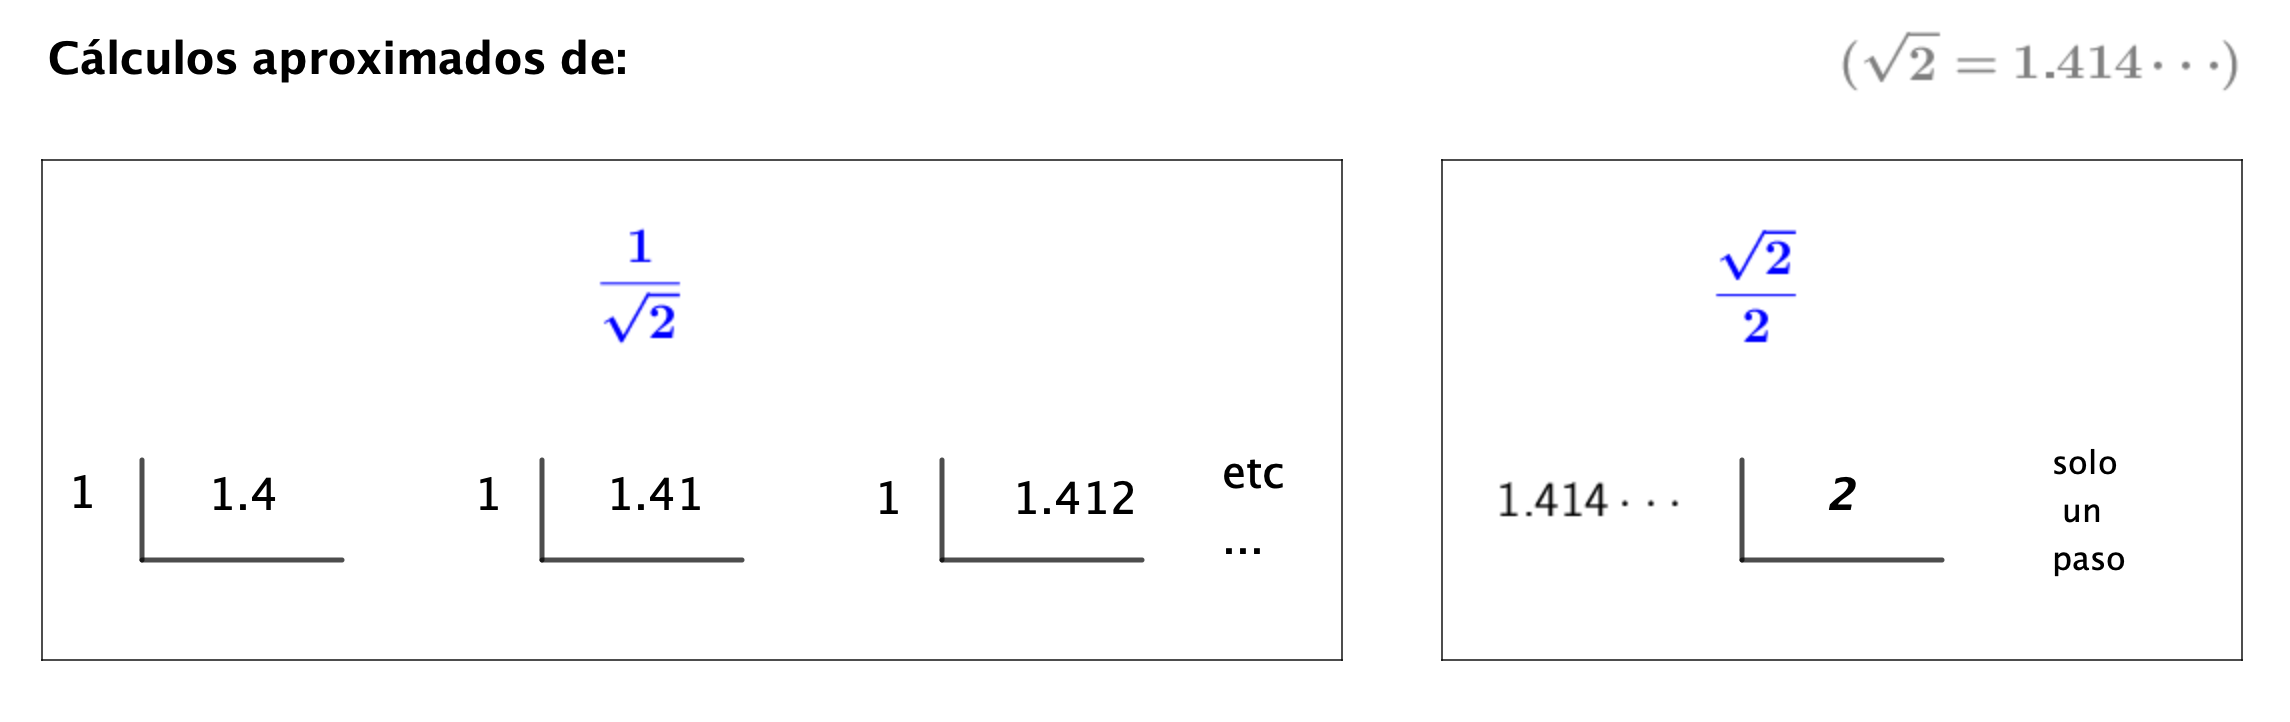
\includegraphics[width=.8\textwidth]{img-reales/reales19.png}
	\end{figure}

De todas formas, el proceso de racionalización es lo suficientemente importante para aprenderlos pues sus técnicas (multiplicar numerador y denominador por la expresión \emph{conjugada}) se usa en la simplificación de muchas expresiones algebraicas.

\vspace{5mm}
$\triangleright\quad$ Expresiones con solo un radical en el denominador:  hay que multiplicar y dividir por la cantidad adecuada para que el denominador se convierta en una expresión del tipo $\ \sqrt[n]{a^n}=a$ 

\begin{miejemplo}

\begin{small}
$\boldsymbol{ \dfrac{3}{2\sqrt{5}} }	\ = \dfrac{3}{2\sqrt{5}}\dfrac{\sqrt{5}}{\sqrt{5}}=\dfrac{3\sqrt{5}}{2(\sqrt{5})^2}=\ \boldsymbol{\dfrac{3\sqrt{5}}{10}}$
$;\qquad \ \ $
$\boldsymbol{ \dfrac{2}{ \sqrt[5]{25} } } = \  \dfrac{2}{ \sqrt[5]{5^2} } = \dfrac{2}{ \sqrt[5]{5^2} } \dfrac{\sqrt[5]{5^3}}{\sqrt[5]{5^3}}=\dfrac{2\sqrt[3]{5^3}}{\sqrt[3]{5^5}} =\ \boldsymbol{ \dfrac{2\sqrt[3]{5^3}}{5} }$\end{small}
\end{miejemplo}

\vspace{5mm}
$\triangleright\quad$ \normalsize{Expresiones} con suma o resta de dos raíces cuadradas en el denominador: se multiplicará y dividirá la fracción por la \emph{expresión conjugada} del denominador (el conjugado de una suma es una resta y viceversa). Se consigue así tener el producto de una suma por diferencia en el denominador que, al ser una diferencia de cuadrados, elimina las raíces cuadradas.

\begin{miejemplo}

\begin{small}$\boldsymbol{\dfrac{2}{2\sqrt{2}-\sqrt{5}}}\ = \dfrac{2}{2\sqrt{2}-\sqrt{5}}\,  \dfrac{2\sqrt{2}+\sqrt{5}}{2\sqrt{2}+\sqrt{5}} = \dfrac{2(2\sqrt{2}+\sqrt{5})}{(2\sqrt{2})^2-(\sqrt{5})^2}=\dfrac{2(2\sqrt{2}+\sqrt{5})}{2^2\cdot 2-5} \ = \boldsymbol{\dfrac{4\sqrt{2}+2\sqrt{5}}{3}}$	\end{small}
\end{miejemplo}
\vspace{5mm}

\begin{myexampleblock}{Raíz de \emph{Ramanujan}}

\begin{figure}[H]
	\centering
	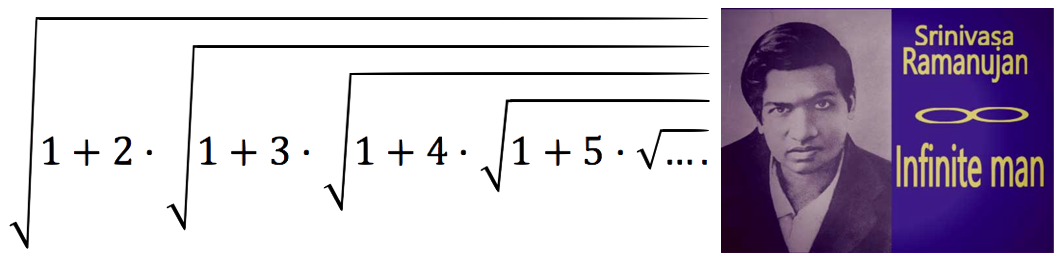
\includegraphics[width=1\textwidth]{img-reales/reales17.png}
	\end{figure}

\vspace{2mm}
\begin{multicols}{2}
	
	$3=\sqrt{9}$
	
	$=\sqrt{1+8}=$
	
	$=\sqrt{1+2\cdot 4}=$
	
	$=\sqrt{1+2\sqrt{16}}=$
	
	$=\sqrt{1+2\sqrt{1+15}}=$
	
	$=\sqrt{1+2\sqrt{1+3\cdot 5}}=$
	
	$=\sqrt{1+2\sqrt{1+3\sqrt{25}}}=$
	
	$=\sqrt{1+2\sqrt{1+3\sqrt{1+4\cdot 6}}}=$
	
	$=\sqrt{1+2\sqrt{1+3\sqrt{1+4\sqrt{36}}}}=$
	
	$=\sqrt{1+2\sqrt{1+3\sqrt{1+4\sqrt{1+\cdots}}}}$

\end{multicols}

\vspace{2mm}
Srinivasa Ramanujan Iyengar o simplemente como Ramanujan (1887-1920), fue un matemático autodidacta indio que, con una mínima educación académica en matemáticas puras, hizo contribuciones extraordinarias al análisis matemático, la teoría de números, las series y las fracciones continuas. Ramanujan desarrolló inicialmente su propia investigación matemática en forma aislada, que fue rápidamente reconocida por los matemáticos indios. Cuando sus habilidades se hicieron evidentes para una comunidad matemática más amplia, centrada en Europa en ese momento, comenzó su famosa colaboración con el matemático británico G. H. Hardy. Redescubrió teoremas conocidos previamente, además de formular numerosas nuevas proposiciones.

\vspace{2mm}

El número $1729$ se conoce como el número de Hardy-Ramanujan por una famosa anécdota del matemático británico G. H. Hardy en relación con una visita al hospital para ver a Ramanujan. En palabras de Hardy: ``Recuerdo una vez que fui a verle cuando estaba enfermo en Putney. Había viajado en el taxi número $1729$ y mencioné que me parecía un número poco notable, y que esperaba que esto no fuera un mal presagio. ``!No!'', me respondió, ``!`es un número muy interesante!; es el número más pequeño expresable como la suma de dos cubos de dos maneras diferentes''. En efecto, la cifra tiene dos descomposiciones diferentes: $9^3+{10}^3=1^3+{12}^3=1729$

\vspace{2mm}

\begin{center} \rule{250pt}{0.1pt} \end{center}

\vspace{2mm}

\color{teal}
\textsf{\begin{small}`El hombre que conocía el infinito'  es una película británica biográfica sobre Ramanujan, del director Matthew Brown, estrenada en $2015$. El actor Dev Patel representa a Srinivasa Ramanujan, un matemático hindú que después de crecer en la pobreza en Madrás, India, es admitido a regañadientes en la exclusiva Universidad de Cambridge en el periodo previo a la Primera Guerra Mundial, donde después de salvar situaciones con matemáticos ingleses muy conservadores que al principio no le hacen la vida fácil, reconocen su genio, es elegido miembro de la Sociedad Matemática de Londres y es reconocido como un pionero en teorías matemáticas formuladas guiado por su profesor, G. H. Hardy.\end{small}\normalsize{.}}


\end{myexampleblock}

\color{black}
\vspace{5mm}
\begin{miejercicio}

$\boldsymbol{ \dfrac{1+\sqrt{x}}{1-\sqrt{x}} } \ = 	\dfrac{1+\sqrt{x}}{1-\sqrt{x}}\,  \dfrac{1+\sqrt{x}}{1+\sqrt{x}}=\dfrac{(1+\sqrt{x})^2}{1^2-(\sqrt{x})^2}=\dfrac{1+2\sqrt{x}+x}{1-x} = \ \boldsymbol{\dfrac{1+x+2\sqrt{x}}{1-x}}$
\end{miejercicio}

\begin{miejercicio}

$\boldsymbol{ \dfrac{2}{\sqrt{3}-\sqrt{5}+2\sqrt{7}} } \ = 
\dfrac{2}{(\sqrt{3}-\sqrt{5})+2\sqrt{7}}=
\dfrac{2}{(\sqrt{3}-\sqrt{5})+2\sqrt{7}}\, \dfrac{(\sqrt{3}-\sqrt{5})-2\sqrt{7}}{(\sqrt{3}-\sqrt{5})-2\sqrt{7}}=$

$= \dfrac{2[(\sqrt{3}-\sqrt{5})-2\sqrt{7}]}{(\sqrt{3}-\sqrt{5})^2-(2\sqrt{7})^2}=
 \dfrac{2[\sqrt{3}-\sqrt{5}-2\sqrt{7}]}{3-2\sqrt{15} +5-2^2\cdot 7}=
\dfrac{2[\sqrt{3}-\sqrt{5}-2\sqrt{7}]}{-20-2\sqrt{15} }=  
$

$=\dfrac{\sqrt{3}-\sqrt{5}-2\sqrt{7}}{-10-\sqrt{15} }= \dfrac{-\sqrt{3}+\sqrt{5}+2\sqrt{7}}{10+\sqrt{15} } \, \dfrac{10-\sqrt{15}}{10-\sqrt{15}}= 
\dfrac{(10+\sqrt{15})(-\sqrt{3}+\sqrt{5}+2\sqrt{7})}{10^2-(\sqrt{15})^2 }=$

$=\ \boldsymbol{
\dfrac{(10+\sqrt{15})(-\sqrt{3}+\sqrt{5}+2\sqrt{7})}{85 } }
\quad $ \begin{footnotesize}
 (faltaría multiplicar el numerador)	
 \end{footnotesize}

\end{miejercicio}

\vspace{10mm}

\begin{myalertblock}{ Racionalizaciones más complejas (ampliación)}
	
\begin{multicols}{3}
Denominador

$\quad \sqrt[n]{a}$

$\quad \sqrt{a} \pm \sqrt{b}$

$\quad \sqrt[3]{a} \pm \sqrt[3]{b}$

Factor racionalizante

$\quad \sqrt[n]{a^{n-m}}$ 

$\quad \sqrt{a} \mp \sqrt{b}$

$\quad \sqrt[3]{a^2} \mp \sqrt[3]{ab} + \sqrt[3]{b^2}$

Denominador racionalizado

$\qquad \qquad a$

$\qquad \qquad a-b$

$\qquad \qquad a\pm b$
	
\end{multicols}




\textcolor{gris}{En la última fila hemos usado que $\ \ (x\pm y)\cdot(x^2\mp xy+y^2) \ = \ x^3\pm y^3$ y hemos sustituido $x$ e $y $ por $\sqrt[3]{a}$ y  $\sqrt[3]{b}$, respectivamente.}

\vspace{2mm} En general:

$$(\sqrt[n]{a}-\sqrt[n]{b})\cdot (\sqrt[n]{a^{n-1}}+\sqrt[n]{a^{n-2}b}+\cdots + \sqrt[n]{b})=a-b $$

$$(\sqrt[n]{a}+\sqrt[n]{b})\cdot (\sqrt[n]{a^{n-1}}-\sqrt[n]{a^{n-2}b}+\cdots + \sqrt[n]{b}) \ = \ \begin{cases}\  a+b& n \text{ impar} \\ \  a-b& n \text{ par} \end{cases}$$

Un factor es el factor racionalizante del otro.

\vspace{2mm}\underline{ejemplos}: 

\vspace{2mm} \begin{small}$\dfrac{2}{\sqrt[3]{4}-\sqrt[3]{2}}=\dfrac{2}{\sqrt[3]{4}-\sqrt[3]{2}}\cdot \dfrac{\sqrt[3]{4^2}+\sqrt[3]{4\cdot 2}+\sqrt[3]{2^2}}{\sqrt[3]{16}+\sqrt[3]{8}+\sqrt[3]{4}}=\dfrac{2(\sqrt[3]{16}+\sqrt[3]{8}+\sqrt[3]{4})}{(\sqrt[3]{4})^3-(\sqrt[3]{2})^3}=\dfrac{\cancel{2} ((\sqrt[3]{16}+\sqrt[3]{8}+\sqrt[3]{4})}{\cancel{2}}$\end{small}




\vspace{2mm} $\dfrac{1}{\sqrt[5]{2}-1}=\dfrac{1}{\sqrt[5]{2}-1} \cdot \dfrac{\sqrt[5]{2^4}+\sqrt[5]{2^3}+\sqrt[5]{2^2}+\sqrt[5]{2}+1}{\sqrt[5]{2^4}+\sqrt[5]{2^3}+\sqrt[5]{2^2}+\sqrt[5]{2}+1} = \dfrac{\sqrt[5]{2^4}+\sqrt[5]{2^3}+\sqrt[5]{2^2}+\sqrt[5]{2}+1}{(\sqrt[5]{2})^5-1}=\sqrt[5]{16}+\sqrt[5]{8}+\sqrt[5]{4}+\sqrt[5]{2}+1$	

\vspace{2mm} $\dfrac{1}{\sqrt[3]{4}-\sqrt[3]{2}+1}=\dfrac{1}{\sqrt[3]{4}-\sqrt[3]{2}+\sqrt[3]{1}} \cdot \dfrac{{\sqrt[3]{2}+1}}{{\sqrt[3]{2}+1}}= \dfrac{\sqrt[3]{2}+1}{(\sqrt[3]{2})^3-(\sqrt[3]{1})^3}=\sqrt[3]{2}+1$
	
\vspace{5mm} \begin{large} \underline{Radicales dobles}:\end{large}

\vspace{2mm} $\boxed{ \subrayado{ \ \boldsymbol{ \sqrt{a \pm \sqrt{b}}\ = \ \sqrt{\dfrac{a+c}{2}} \pm \sqrt{\dfrac{a-c}{2}} } \  }  } \, ;\qquad a,b>0$

\color{gris}
\vspace{4mm}\underline{demostración}:

\vspace{2mm} llamando $\ \sqrt{a+\sqrt{b}}=\sqrt{x}+\sqrt{y} \ \text{ y } \ \sqrt{a-\sqrt{b}}=\sqrt{x}-\sqrt{y}$,

\vspace{2mm} sumando $\ \sqrt{a+\sqrt{b}}+ \sqrt{a-\sqrt{b}}=2\sqrt{x}$

\vspace{2mm} elevando al cuadrado $\ a+\cancel{\sqrt{b}}+a-\cancel{\sqrt{b}}+2\sqrt{a^2-b}=4x \ \to \ x=\dfrac{a+\sqrt{a^2-b}}{2}$

\vspace{2mm} \emph{condición}: $\ a^2-b=c^2\, , \ $ cuadrado perfecto!

\vspace{2mm} restando $\ \sqrt{a+\sqrt{b}}- \sqrt{a-\sqrt{b}}=2\sqrt{y} $

\vspace{2mm} y por el mismo procedimiento $ y=\dfrac{a-\sqrt{a^2-b}}{2}$

\vspace{2mm} con lo que $\ \sqrt{a \pm \sqrt{b}}\ = \ \sqrt{\dfrac{a+c}{2}} \pm \sqrt{\dfrac{a-c}{2}}\, \ \text{ con } \ c=\sqrt{a^2-b} $ \QED

\color{black}
\vspace{2mm}\underline{ejemplos}: 

\vspace{2mm} $\sqrt{7+\sqrt{40}}=\left[\mqty{a=7\\b=40} \  \right| \left. \ c=\sqrt{7^2-40}=3 \right] = \sqrt{\dfrac{7+3}{2}}+\sqrt{\dfrac{7-3}{2}}=\sqrt{5}+\sqrt{2}$

\vspace{2mm}  $\sqrt{12-\sqrt{108}}=\left[\mqty{a=12\\b=102} \  \right| \left. \ c=\sqrt{12^2-108}=6 \right] = \sqrt{\dfrac{12+6}{2}}-\sqrt{\dfrac{12-6}{2}}=3-\sqrt{3}$


\vspace{5mm} $\boxed{ \subrayado{ \ \boldsymbol{ 
\sqrt{S\pm 2\sqrt{P}} \ = \ \sqrt{a}  \pm \sqrt{b}
} \ } } \, ;\qquad a,b>0;\quad S=a+b;\ P=a\cdot b$

\color{gris}
\vspace{4mm}\underline{demostración}:

\vspace{2mm} $(\sqrt{a}\pm \sqrt{b})^2=a+b\pm 2\sqrt{ab}=S\pm 2\sqrt{P}\, ; \quad S=a+b;\ P=a\cdot b$

\vspace{2mm} \normalsize{sacando} raíz cuadrada $\ |\sqrt{a} \pm \sqrt{b}| = \sqrt{S\pm 2\sqrt{P}}$

\color{black}
\vspace{2mm}\underline{ejemplos}: 

\vspace{2mm} $\sqrt{9+\sqrt{80}}=\sqrt{9+2\sqrt{20}} =
\left[ \mqty{S=9\\P=20} \ \right| \left. \  \mqty{a=5\\b=4} \right]=\sqrt{5}+\sqrt{4}=\sqrt{5}+2$

\vspace{2mm} $\sqrt{7-\sqrt{48}}=\sqrt{7-2\sqrt{12}} =
\left[ \mqty{S=7\\P=12} \ \right| \left. \  \mqty{a=4\\b=3} \right]=\sqrt{4}-\sqrt{3}=2-\sqrt{3}$

\color{gris}

\vspace{4mm}Como ejercicio, probar que:

\vspace{2mm} $\qquad \sqrt{\sqrt{38+12\sqrt{2}} + \sqrt{26-8\sqrt{3}}+1}= \ \cdots \ = \sqrt{6}+1$

\vspace{2mm} $\qquad \sqrt{9+2\sqrt{7+6\sqrt{6+4\sqrt{2}}}}= \ \cdots \ = 3+\sqrt{2}$
\color{black}	
\end{myalertblock}

\vspace{5mm}
\begin{figure}[H]
	\centering
	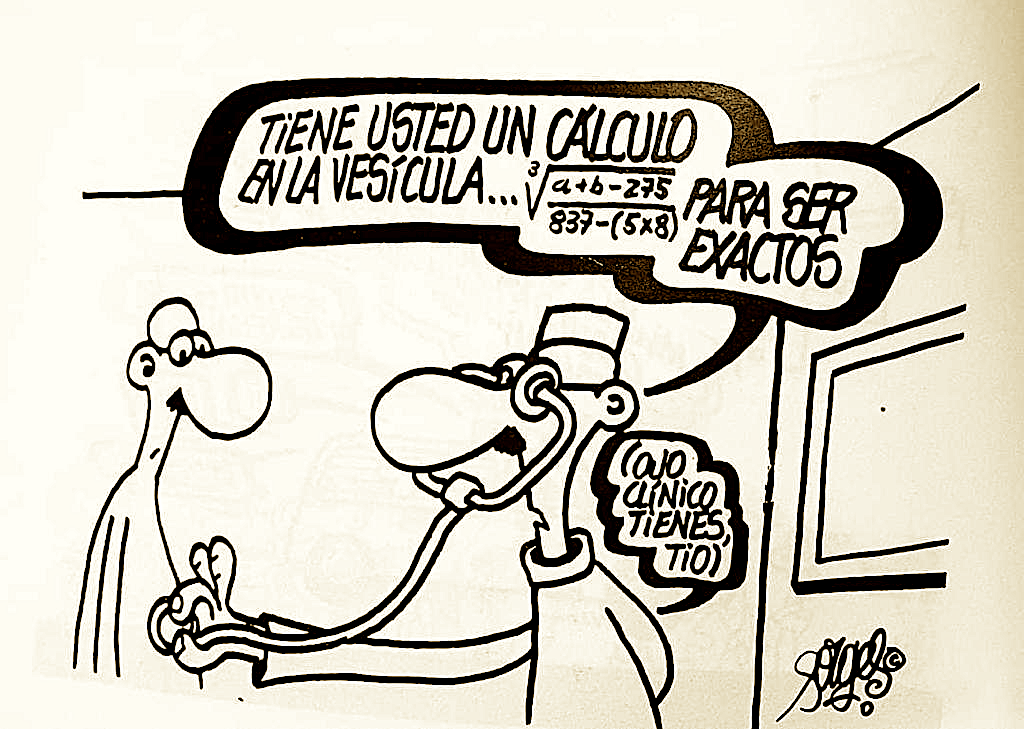
\includegraphics[width=.75\textwidth]{img-reales/reales21.png}
	\end{figure}

\vspace{1cm}
\section{Logaritmos}
\begin{tikzpicture}
	\fill [left color=red!50, right color=teal!50] (0,0) rectangle (3.5,.1);
	\fill [left color=teal!50, right color=blue!50] (3.5,0) rectangle (7.5,.1);
	\end{tikzpicture}
\vspace{0.5cm}


\begin{myexampleblock}{Escala logarítmica y órdenes de magnitud}
	
La utilidad fundamental de los logaritmos radica en manejar `escalas logarítmicas’. 

\vspace{2mm} Una escala logarítmica es una escala de medida que utiliza el logaritmo de una cantidad física en lugar de la propia cantidad.

\vspace{2mm} Un ejemplo sencillo de escala logarítmica muestra divisiones igualmente espaciadas en el eje vertical de un gráfico marcadas con 1, 10, 100, 1000, …, en vez de 0, 1, 2, 3, …

\vspace{2mm} La presentación de datos en una escala logarítmica es muy útil cuando los datos cubren una amplia gama de valores - el logaritmo los reduce a un rango más manejable.

\vspace{2mm} Ejemplos de escalas logarítmicas son:

--- Cuando hablamos del PH , que es una concentración media según una escala logarítmica.

--- Cuando medimos la intensidad de los terremotos de acuerdo a la escala Richter.

--- Cuando hablamos del brillo de las estrellas (magnitud aparente).

--- La intensidad del sonido (Decibelios) también es una escala logarítmica.

\vspace{2mm}
Se basan en órdenes de magnitud, en lugar de una escala lineal estándar. El valor de cada marca de la escala es 10 veces la marca anterior (logaritmos decimales). Se utilizan órdenes de magnitud para hacer comparaciones aproximadas. Si los números difieren en un orden de magnitud, x es aproximadamente diez veces diferente en cantidad que y . Si los valores difieren en dos órdenes de magnitud, difieren en un factor de aproximadamente 100. Dos números del mismo orden de magnitud tienen aproximadamente la misma escala: el valor mayor es menos de diez veces el valor menor.

\underline{Escala logarítmica}

\begin{multicols}{2}
$\quad$

La imagen muestra cómo podría realizarse un mapa a escala logarítmica de todo el Universo visible, de manera que -al igual que ocurre con los mapas terrestres- preserve a pequeña escala las formas, mostrando a la vez todo el rango de distancias astronómicas (desde el espacio local, cercano a la Tierra, hasta los objetos situados a escala cosmológica como los quasars).
\begin{figure}[H]
	\centering
	\includegraphics[width=0.4\textwidth]{img-reales/reales12.png}
	\end{figure}
\end{multicols}

\underline{Órdenes de magnitud}
\begin{figure}[H]
	\centering
	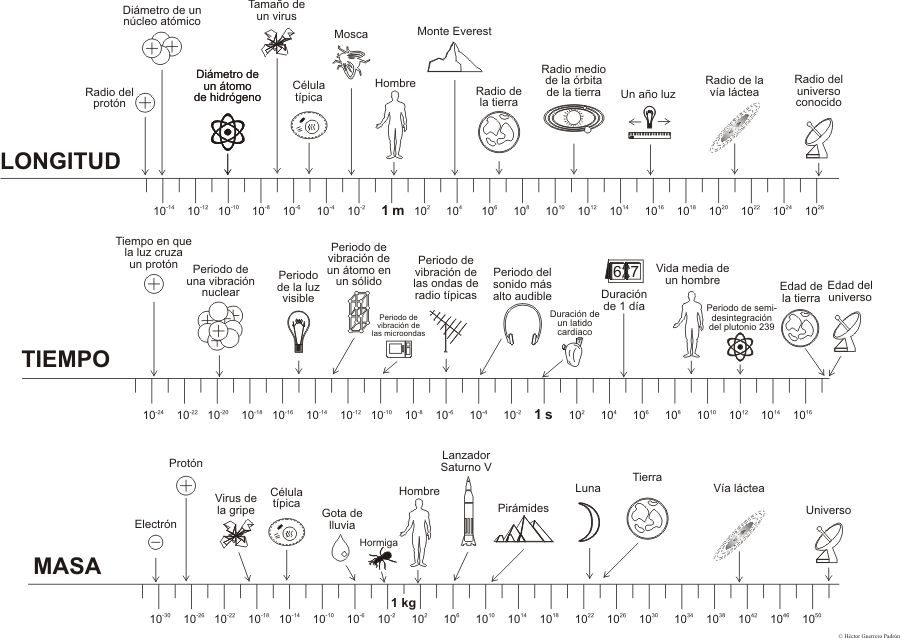
\includegraphics[width=1\textwidth]{img-reales/reales14.png}
	\end{figure}

\end{myexampleblock}

\color{teal}
\rule{250pt}{0.1pt}	

A partir del siglo XVI, los cálculos que se precisaban hacer, debido principalmente a la expansión comercial y al perfeccionamiento de las técnicas de navegación, eran de tal magnitud que surgía la necesidad de encontrar algoritmos que los facilitasen. 

\vspace{3mm} Los logaritmos fueron introducidos por John Napier a principios del siglo XVII como un medio de simplificación de los cálculos y fueron prontamente adoptados por científicos, ingenieros, banqueros y otros para realizar operaciones fácil y rápidamente. Los logaritmos permitían transformar los productos en sumas y los cocientes en restas con lo que la facilidad del cálculo quedaba garantizada. Aún más, los logaritmos transformas potencias (y raíces) en meros productos por el exponente. 

\vspace{3mm} Hoy día, su utilidad radica en la sencillez que proporciona su uso en muchas expresiones simbólicas y en el uso de escalas logarítmicas.

\begin{center}
\rule{200pt}{0.1pt}	
\end{center}

\vspace{-3mm} En ciencia se acostumbra a trabajar con números muy grandes: 

\hspace{5mm} --- Masa del Sol, $M_{\sun}= 1984000000000000000000000000000000\, $ kg.

\hspace{5mm} --- Masa del electrón, $m_{e^{-}}=0.000000000000000000000000000000911\, $ kg. 

\vspace{2mm} Para esto se usa la \underline{\emph{notación científica}}, $\boldsymbol{m \times 10^e}$; $m\in [1,10[ $ es la mantisa y $e$ el exponente de base 10. Así,
$\ 243000000000=2.43\times 10^{11} \, ; \qquad 0.000008724=8.274\time 10^{-6}$

\vspace{-5mm}
\begin{flushright}
\rule{250pt}{0.1pt}	
\end{flushright}
\color{black}
\vspace{5mm}


\begin{definition}[ Logaritmos]

\begin{multicols}{2}
Sea $\ a>0\, , \ a\neq 1\, , \ $  	llamamos \emph{logaritmo} en base $ \ a \ $ de un número $ \ P \ $ , y lo denotamos por $\ \log_aP \, , \ $ al número al que hay que elevar $\ a \ $ para obtener $\ P \, . $

$$
\boxed{ \ \boldsymbol{
\log_a P \ = \ b \ \leftrightarrow \ a^P\ = \ b
} \ }
$$

$\quad$
\begin{figure}[H]
	\centering
	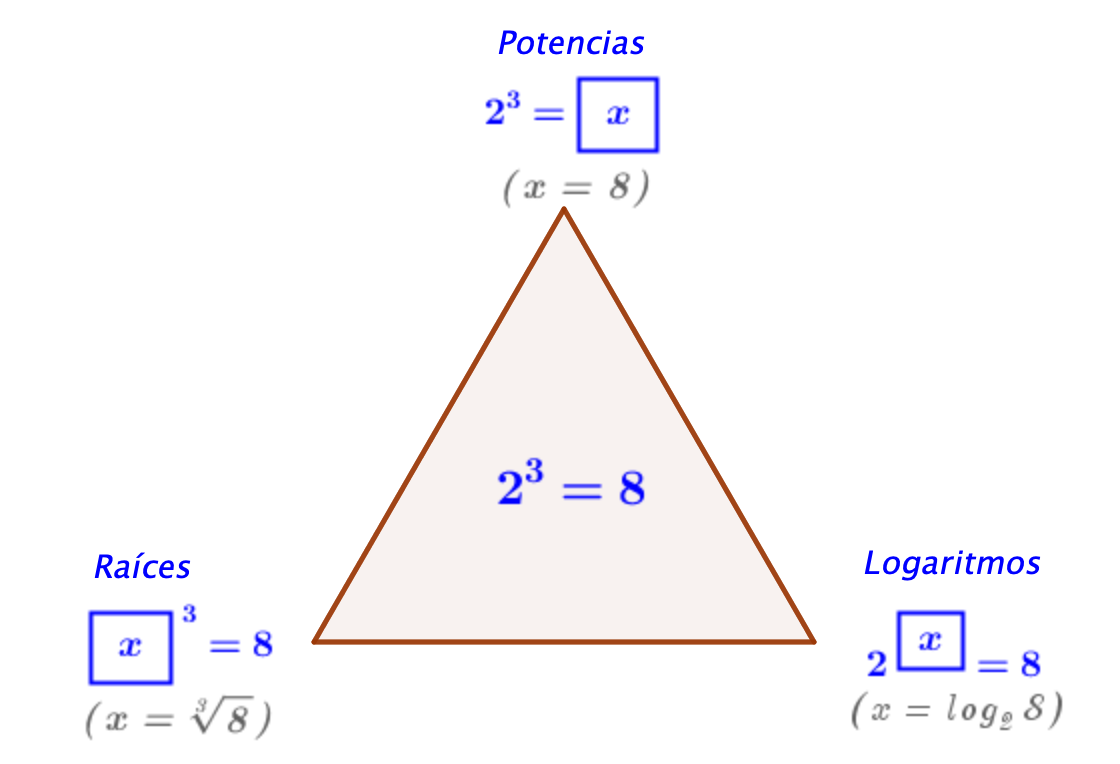
\includegraphics[width=0.5\textwidth]{img-reales/reales13.png}
	\end{figure}
\end{multicols}
\end{definition}


\begin{miejemplo}

$\log_28=3 \leftrightarrow 2^3=8;\quad \log_525=2 \leftrightarrow 5^2=25;\quad \log_{10}0.0001 =-4 \leftrightarrow 10^{-4}=0.0001$	
\end{miejemplo}

\vspace{5mm}

\begin{theorem}[ Propiedades de los logaritmos]
	
	\begin{enumerate}[P1. ]
	\item $\boldsymbol{ \log_aa=1}$
	
	\textcolor{gris}{$\log_aa=b \ \leftrightarrow \ a^b=1 \ \to \ b=1$ \QED} 	
	
	\item $\boldsymbol{\log_a1=0}$
	
	\textcolor{gris}{$\log_a1=b \ \leftrightarrow \ a^b=1 \ \to \ b=0$ \QED} 	
	
	\item $\boldsymbol{\log_a (A\cdot B)\ = \ \log_aA\ + \ \log_aB }\quad $ El log. del producto la suma de log.

\color{gris}
	\small{	
	$\begin{cases}
	\ \log_a(A\cdot B)=b \ \leftrightarrow \ a^b=A\cdot B \\
	\ \log_aA=b_1 \ \leftrightarrow \ a^{b_1}=A	\\
	\ \log_aB=b_2 \ \leftrightarrow \ a^{b_2}=B
	\end{cases}
	a^b=A\cdot B=a^{b_1}a^{b_2}=a^{b_1+b_2} \ \to \ b=b_1+b_2 $ \QED }	
	\color{black} 
	
	\item $\boldsymbol{\log_a \left(\dfrac A B \right)\ = \ \log_aA\ - \ \log_aB }\quad $ El log. del cociente la resta de log\normalsize{.}
	
	\color{gris}
	\small{	
	$\begin{cases}
	\ \log_a(A/ B)=b \ \leftrightarrow \ a^b=A/B \\
	\ \log_aA=b_1 \ \leftrightarrow \ a^{b_1}=A	\\
	\ \log_aB=b_2 \ \leftrightarrow \ a^{b_2}=B
	\end{cases}
	a^b=A/ B=a^{b_1}/a^{b_2}=a^{b_1-b_2} \ \to \ b=b_1-b_2 $ \QED }	
	\color{black} 
	
	\item $\boldsymbol{\log_a (A^n)\ = \ n\cdot \log_aA} \quad $ \small{El log. de una potencia es el exponente por el log de la base}\normalsize{.}
	
	\color{gris}{
		\small{	
	$\begin{cases}
	\ \log_a(A^n)=b \ \leftrightarrow \ a^b=A^n \\
	\ \log_aA=b_1 \ \leftrightarrow \ a^{b_1}=A	\\
	\end{cases}
	a^b=A^n=(a^{b_1})^n=a^{n\, b_1}\ \to \ b=n\, b_1 $ \QED }	}
	\color{black} 

\end{enumerate}

\end{theorem}

De la última propiedad deducimos que el logaritmo de una raíz es el logaritmo del radicando dividido por el índice de la raíz:
$\quad \boldsymbol{ \log_a \sqrt[n]{A} }\ = \log_a A^{1/n} = \ (P5) \ = \frac 1 n \, \log_a A=\ \boldsymbol{ \dfrac{\log_aA}{n} }$ 


\begin{figure}[H]
	\centering
	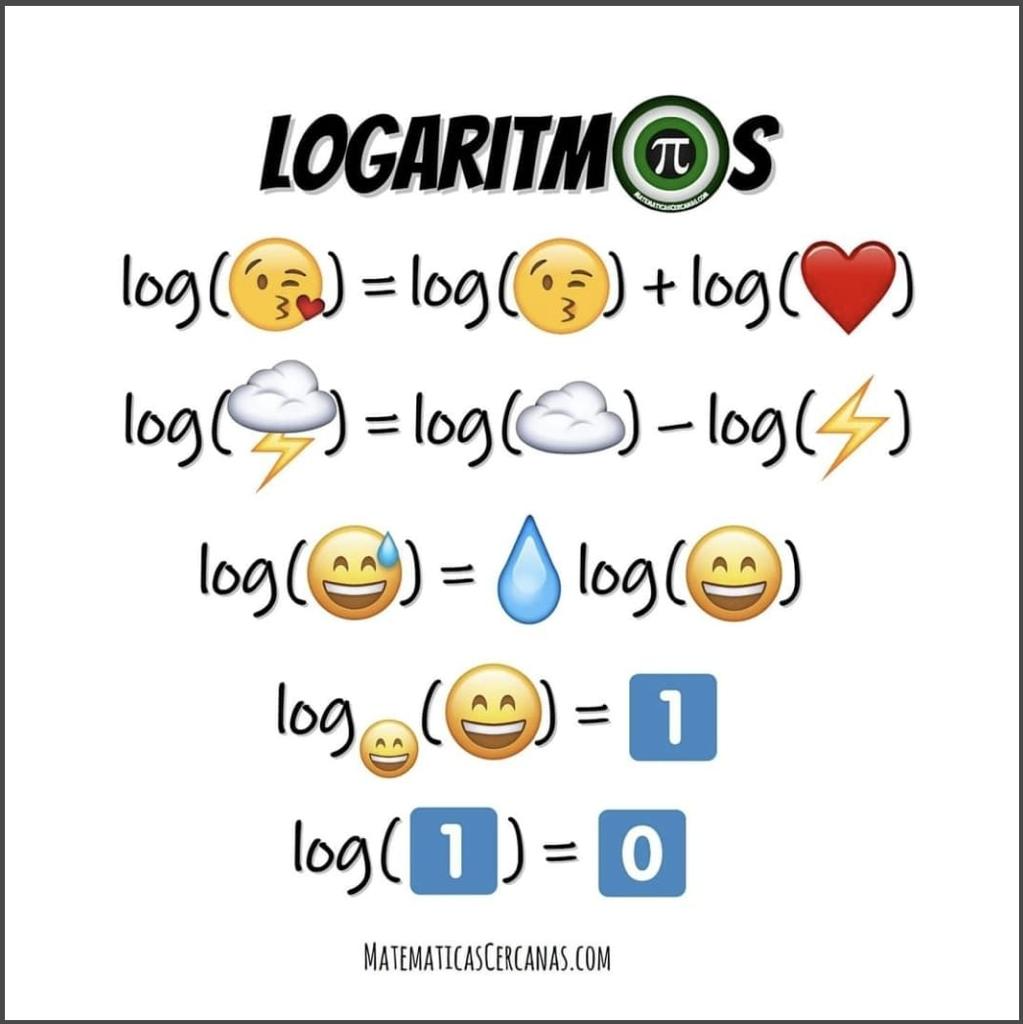
\includegraphics[width=0.4\textwidth]{img-reales/reales20.png}
	\end{figure}


\vspace{5mm}

\begin{theorem}[ Cambio de base en logaritmos]
	
	$$\boxed{\ \boldsymbol{ \log_aP\ = \ \dfrac{\log_c P}{\log_c a} } \ \ }$$
\end{theorem}

\underline{Demostración} 

$\log_aP=b\ \leftrightarrow \ a^b=P\, ,  $ tomemos logaritmos en otra base, $ \ c\ $ por ejemplo:

$\log_c (a^b) = \log_c P \, $ aplicando la propiedad P5 de los logaritmos,

$b\, \log_c a = \log_c P \ \to \ b=\dfrac{\log_c P}{\log_c a} \, $ pero $\ b=\log_aP\, , \  $ luego

$\log_aP\ = \ \dfrac{\log_c P}{\log_c a}$ \QED

\vspace{5mm}

Como $\log_aP=b \leftrightarrow P=a^b>0$, un número positivo $a$ elevado a cualquier número $b$ siempre es positivo, \emph{el logaritmo solo se puede calcular para número estrictamente positivos} (el dominio de la función logarítmica es $\mathbb R^+$). Al poder ser $b$ cualquier número real, \emph{el logaritmo de un número positivo puede ser cualquier número real, positivo, negativo o nulo} (el recorrido de la función logarítimca es $\mathbb R$). 

\vspace{5mm}

Con una sola base que tuviésemos de logaritmos sería más que suficiente. En las calculadoras aparecen los logaritmos más usuales que son los \emph{logaritmos decimales}, de base $10$, y los \emph{logaritmos neperianos} o \emph{naturales} cuya base es el número $\ e\,\approx \, 2.7182\cdots\,  $. 
Sus representaciones son: 
$\qquad \log_{10} \ \equiv \ \boldsymbol{ Log} \, ; \qquad  \log_e\ \equiv \boldsymbol{ \ln}$


\vspace{5mm}

\begin{adjustwidth}{100pt}{100pt}
\begin{cuadro-naranja}
$$\boldsymbol{ \log_a a^x\ = \ x \qquad 	 \qquad  \qquad  a^{\log_a x}\ = \ x }$$

\vspace{1mm}
\end{cuadro-naranja}
\end{adjustwidth}

\color{gris}
\underline{Demostracines}:

$\log_a^x=x\cancelto{1}{\log_a a}=x$ \QED

$a^{\log_a x}=P\ $ tomamos logaritmos, $\ \log_a{a^{\log_a x}}=\log_a P;\ \ \log_a x\cdot \cancelto{1}{\log_a a}=\log_a P \ \to \ x=P$ \QED
\color{black}

\vspace{5mm}
\begin{miejercicio}

Calcula los siguientes logaritmos aplicando la definición:

\vspace{2mm} $\log_2 1024; \qquad \log_2 0.5;\qquad \log_5 125;\qquad	 \log_{\frac 1 3}\frac 1 9;\qquad \log_4 \sqrt{2}$

\rule{300pt}{0.1pt}

$\triangleright \quad \log_2 1024=x \ \leftrightarrow \ 2^x=1024=2^{10} \ \to \ x= \ \boldsymbol{ \log_2 1024=10 }$

\vspace{2mm} $\triangleright \quad \log_2 0.5=x \ \leftrightarrow \ 2^x=0.5=\frac 1 2 =2^{-1} \ \to \ x=\ \boldsymbol{\log_2 0.5=-1}$

\vspace{2mm} $\triangleright \quad \log_5 125=x \ \leftrightarrow \ 5^x=125=5^3 \ \to \ x=\ \boldsymbol{\log_5 125=3}$

\vspace{2mm} $\triangleright \quad \log_{\frac 1 3} \frac 1 9 = x \ \leftrightarrow \ \left( \frac 1 3 \right)^x=\frac 1 9 = \left( \frac 1 3 \right)^2 \ \to \ x=\ \boldsymbol {\log_{\frac 1 3} \frac 1 9 = 2}$

\vspace{2mm} $\triangleright \quad \log_4 \sqrt{2}=x \ \leftrightarrow \ 4^x=\sqrt{2} \ \to {(2^2)}^x=2^{\frac 1 2 } \ \to \ 2x=\frac 1 2 \ \to \ x=\ \boldsymbol{\log_4 \sqrt{x}=\frac 1 4}$
\end{miejercicio}


\begin{miejercicio}

Encuentra la base de los siguientes logaritmos:

\vspace{2mm} $\log_a 243=5;\qquad \log_a 0.125=3;\qquad \log_a 0.001=-3;\qquad \log_a 3=2;\qquad \log_a \sqrt[4]{5}=\frac 1 2 $	

\rule{300pt}{0.1pt}

$\log_a 243=5 \ \leftrightarrow \ a^5=243=3^5 \ \to \boldsymbol{ a}= \sqrt[5]{243} =\boldsymbol{ 5}$

\vspace{2mm} $\log_a 0.125=3 \ \leftrightarrow \ a^3=0.125=\frac 1 8 =2^{-3}=\left( \frac 1 2 \right)^3 \ \to \ \boldsymbol{a}=\sqrt[3]{125}=\boldsymbol{ \frac 1 2}$

\vspace{2mm} $\log_a 0.001=-3 \ \leftrightarrow \ a^{-3}=0.001=10^{-3} \ \to \ \boldsymbol{a}= 0.001^{-1/3}= \frac 1 {\sqrt[3]{0.001}}=\boldsymbol {10}$

\vspace{2mm} $\log_a 3=2 \ \leftrightarrow \ a^2=3 \ \to \ a^2=(\sqrt{3})^2 \ \to \ \boldsymbol{a}=\sqrt{3} =\boldsymbol{\sqrt{3}}$
\end{miejercicio}

\begin{miejercicio}

Calcula: $\qquad 3^{1/x}=9;\qquad \log_{16}0.5=x;\qquad \log_{10}0.00001=x;\qquad log_x 125=\frac 32$	


\rule{300pt}{0.1pt}

$3^{1/x}=9=3^2 \ \to \ \frac 1 x = 2 \ \to \ 1=2x \ \to \ \boldsymbol{x=\frac 1 2} $

\vspace{2mm} $\log_{16}0.5=x \ \leftrightarrow \ 16^x=0.5=\frac 1 2 \ \to \ (2^4)^x=2^{4x}=2^{-1} \ \to \ 4x=-1 \ \to \ \boldsymbol{x=-\frac 1 4}$

\vspace{2mm} $\log_{10}0.00001=x \ \leftrightarrow \ 10^x=0.00001=10^{-5} \ \to \ \boldsymbol{x=-5}$

\vspace{2mm} $log_x 125=\frac 32 \ \leftrightarrow \ x^{3/2}=125=5^3 \ \to \ \boldsymbol{x}=(x^{3/2})^{2/3}=(5^3)^{2/3}=5^2=\boldsymbol{25}$	
 \end{miejercicio}
 


\begin{miejercicio}

Calcula: $\qquad \log_3 1 +\log_2 64 +\log_3 9 + \log_7 49$	


\rule{300pt}{0.1pt}

$\log_3 1 +\log_2 64 +\log_3 9 + \log_7 49=\cancelto{0}{\log_3 1} +\log_2 2^6 +\log_3 3^2 + \log_7 7^2=0 +6 \cancelto{1}{\log_2 2} +2 \cancelto{1}{\log_3 3} + 2 \cancelto{1}{\log_7 7}=6+2+2=\boldsymbol{ 10}$

\end{miejercicio}


\begin{miejercicio}

Calcula $x:\qquad \ln x=\ln 3+\ln 2-\ln 6;\qquad \mathrm{Log}x	=3\mathrm{Log}2-\frac 1 4 \mathrm{Log}16$

\rule{300pt}{0.1pt}

$\triangleright \quad \ln x=\ln 3+\ln 2-\ln 6=\ln(3\cdot 2)-\ln 6=\ln\left( \dfrac {3\cdot 2}{6} \right)=\ln 1 \ \to \ \boldsymbol{x=1} $

\vspace{2mm} $\triangleright \quad \mathrm{Log}x	=3\mathrm{Log}2-\frac 1 4 \mathrm{Log}16 \ \to \ \mathrm{Log} x= \mathrm{Log}2^3-\mathrm{Log}16^{1/4}= \mathrm{Log} \left( \dfrac{2^3}{\sqrt[4]{16}} \right)=\mathrm{Log} \dfrac 8 2 = \mathrm{Log} 4 \ \to \ \boldsymbol{x=4}$

\end{miejercicio}


\begin{miejercicio}

Desarrolla la siguiente expresión usando las propiedades de los logaritmos.


\rule{300pt}{0.1pt}

\vspace{2mm} $\boldsymbol{ \ln \dfrac{a^2\sqrt[5]{b}}{\sqrt[3]{c^4}}} = \ln(a^2\sqrt[5]{b})-\ln\sqrt[3]{c^4}=\ln a^2 +\ln \sqrt[5]{b}-\ln\sqrt[3]{c^4}=\boldsymbol{ 2\ln a +\frac 1 5 \ln b - \frac 4 3 \ln c }$ 
	
\end{miejercicio}

\begin{miejercicio}

Comprime la expresión siguiente para que el logaritmos aparezca una sola vez.


\rule{300pt}{0.1pt}

\vspace{2mm} $\boldsymbol{3\mathrm{Log} x +\frac 12 \mathrm{Log} (1-x)}=\mathrm{Log} x^3  + \mathrm{Log}  \sqrt{1-x}= \mathrm{Log} \left( x^3\, \sqrt{1-x} \right)$
	
\end{miejercicio}


\vspace{1cm}
\section{Números combinatorios. Binomio de Newton}
\begin{tikzpicture}
	\fill [left color=red!50, right color=teal!50] (0,0) rectangle (3.5,.1);
	\fill [left color=teal!50, right color=blue!50] (3.5,0) rectangle (7.5,.1);
	\end{tikzpicture}
\vspace{0.5cm}

\begin{definition}[ Factorial de un número]
	
	Se llama factorial de un número natural, $n\in \mathbb N$, y se representa por $\boldsymbol{n!}$, al producto de los factores consecutivos que empiezan por la unidad y acaban en $n$:
	
	$$\boldsymbol{ n! \ = \ 1\cdot 2 \cdot 3 \cdot \cdots \cdot (n-2) \cdot (n-1)\cdot n } \ = \ \displaystyle \prod_{k=1}^n k \qquad \text{(productorio)}$$
	
Por convenio, $\ 0!=1\, ; \qquad $ Es evidente que $\ n!=n\cdot (n-1)!$
\end{definition}


\begin{definition}[ Número combinatorio]
	.Se define el \textbf{número combinatorio $\boldsymbol{n}$ sobre $\boldsymbol{k}$}, con $\boldsymbol{n,k \in \mathbb N \, \wedge \ k\le n}$, y se denota por $\boldsymbol{\mqty(n\\k)}$, como:
	
	\vspace{2mm} $$\boxed{\ \boldsymbol{ \mqty(n\\k) \ = \ \textcolor{gris}{C_n^r} \ = \ \dfrac {n!}{k! \cdot (n-k)!} }	 \ }$$
	
	\vspace{2mm} Indican las combinaciones, sin repetición, de $n$-elementos tomados de $k$ en $k$ o el número de subconjuntos de $k$-elementos de un conjunto de $n$-elementos.
\end{definition}

\begin{theorem}[ Propiedades de los números combinatorios]
	. Propiedades de los números combinatorios.
	
	\begin{small}
	$$\mqty(n\\r)=\mqty(n\\n-r); \qquad \mqty(n\\0)=\mqty(n\\n)=1; \qquad \mqty(n\\r)+\mqty(n\\r+1)=\mqty(n+1\\r+1)$$
	\end{small}	
\end{theorem}

\color{gris}
\begin{small}
\underline{demostraciones}:

\vspace{2mm} $\triangleright \quad \mqty(n\\n-r)=\dfrac{n!}{(n-r)![n-(n-r)]!}=\dfrac{n!}{(n-r)!\, r!}=\mqty(n\\r)\ $ \QED


\vspace{2mm} $\triangleright \quad \mqty(n\\0)=\dfrac{n!}{0! \, n!}=1;\qquad \mqty(n\\ n)=\dfrac{n!}{n!(n-n)!}=1\ $ \QED


\vspace{2mm} $\triangleright \quad  \mqty(n\\r)+\mqty(n\\r+1)=\dfrac{n!}{r!(n-r)!}+\dfrac{n!}{(r+1)!(n-r-1)!}= \dfrac{n!(r+1)}{(r+1)!(n-r)!}+\dfrac{n!(n-r)}{(r+1)!(n-r)!}=$

$= \dfrac{n![\cancel{r}+1+n-\cancel{r}]}{(r+1)(n-r)!}=\dfrac{n!(n+1)}{(r+1)![(n+1)-(r+1)!]}=\dfrac{(n+1)!}{(r+1)![(n+1)-(r+1)!]}=\mqty(n+1\\r+1)\ $ \QED

\end{small}

\color{black}

\vspace{5mm}
\begin{miejercicio}

Encuentra el valor de $x$ tal que $\ \mqty(x\\2)=3!$

\vspace{2mm} 
\rule{300pt}{0.1pt}

\vspace{2mm} $\mqty(x\\2)=\dfrac{x!}{2!\cdot (x-2)!}=\dfrac{x\cdot(x-1)\cdot\cancel{ (x-2)!}}{2\, \cancel{(x-2)!}}=\dfrac{x(x-1)}{2}=3!=6 \ \to $

\vspace{2mm} $\to \ x(x-1)=12 \ \to \ x^2-x-12=0 \ \to \begin{cases}
 \ x=-3 \notin \mathbb N \\ \ x\ =\ 4 \in \mathbb N	
 \end{cases} \ \text{ Sol.: } \ \boldsymbol{x=4}$	
\end{miejercicio}

\begin{miejercicio}

Resuelve: $\quad \dfrac{m!}{(m-1)!}=\mqty(m\\2)$
\vspace{2mm} 

\rule{300pt}{0.1pt}	

\vspace{2mm} Al tener $\ \mqty(m\\2) \ \to \ m\in \mathbb N\, , /\ m>2$

\vspace{2mm} $\dfrac{m!}{(m-1)!}= \dfrac{m\cdot \cancel{(m-1)!}}{\cancel{(m-1)!}}=m $

$\mqty(m\\2)=\dfrac{m!}{2!\cdot (m-2)!}=\dfrac{m\cdot (m-1) \cdot \cancel{(m-2)!}}{2\cdot \cancel{(m-2)!}}=\dfrac{m(m-1)}{2} $

\vspace{2mm} $\dfrac{m!}{(m-1)!}=\mqty(m\\2) \ \to \ m=\dfrac{m(m-1)}{2} \ \to \ m^2-3m=m(m-3)=0 \ \to \begin{cases} \ m=0 \not> 2 \\ \ m=3\end{cases}$

\vspace{2mm} Solución: $\ \ \boldsymbol{m=3}$

\end{miejercicio}


\vspace{5mm}
\begin{myexampleblock}{Triángulo de Tartaglia}
	

Disposición de los números combinatorios en el \textbf{Triángulo de Tartaglia}	
	
	
\begin{table}[H]
\centering
\tiny
\begin{tabular}{ccccccccc}
 &  &  & $\mqty(1\\0)$ &  & $\mqty(1\\1)$ &  &  &  \\
 &  & $\mqty(2\\0)$ &  & $\mqty(2\\1)$ &  & $\mqty(2\\2)$ &  &  \\
 & $\mqty(3\\0)$ &  & $\mqty(3\\1)$ &  & $\mqty(3\\2)$ &  & $\mqty(3\\3)$ &  \\
$\mqty(4\\0)$ &  & $\mqty(4\\1)$ &  & $\mqty(4\\2)$ &  & $\mqty(4\\3)$ &  & $\mqty(4\\4)$ \\
$\cdots$ & $\cdots$ & $\cdots$ & $\cdots$ & $\cdots$ & $\cdots$ & $\cdots$ & $\cdots$ & $\cdots$
\end{tabular}
\end{table}

\vspace{-8mm}

\begin{center}
\begin{Large}
\rotatebox{90}{$\equiv$}	
\end{Large}	
\end{center}

\normalsize

\vspace{-8mm}
\begin{table}[H]
\centering
\small
\begin{tabular}{ccccccccc}
 &  &  & 1 &  & 1 &  &  &  \\
 &  & 1 &  & 2 &  & 1 &  &  \\
 & 1 &  & 3 &  & 3 &  & 1 &  \\
1 &  & 4 &  & 6 &  & 4 &  & 1 \\
$\cdots$ & $\cdots$ & $\cdots$ & $\cdots$ & $\cdots$ & $\cdots$ & $\cdots$ & $\cdots$ & $\cdots$
\end{tabular}
\end{table}

\end{myexampleblock}

\begin{figure}[H]
	\centering
	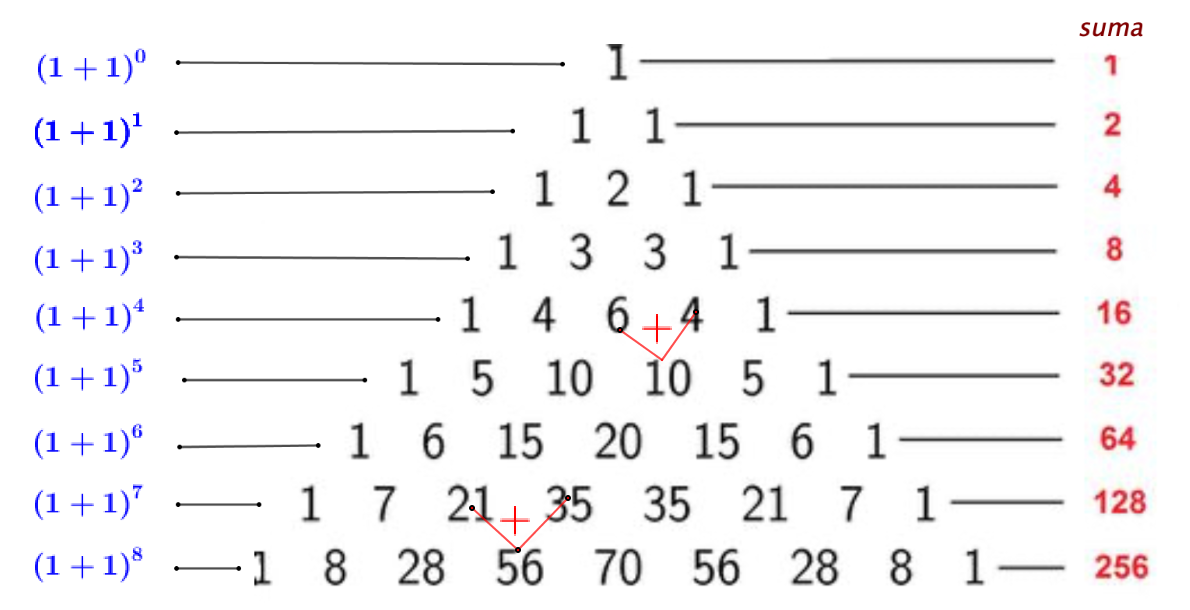
\includegraphics[width=0.75\textwidth]{img-reales/reales15.png}
	\end{figure}


\begin{theorem}[ Binomio de Newton]

$$(a+b)^n  = \mqty(n\\0)a^nb^0+\mqty(n\\1)a^{n-1}b^1+\mqty(n\\2)a^{n-2}b^2+ \cdots \mqty(n\\n-1)a^1b^{n-1}+\mqty(n\\n)a^0b^n $$

\vspace{2mm} Los coeficientes del desarrollo son los números de la fila $n$-ésima de Tartaglia.
	 
\end{theorem}




\begin{figure}[H]
	\centering
	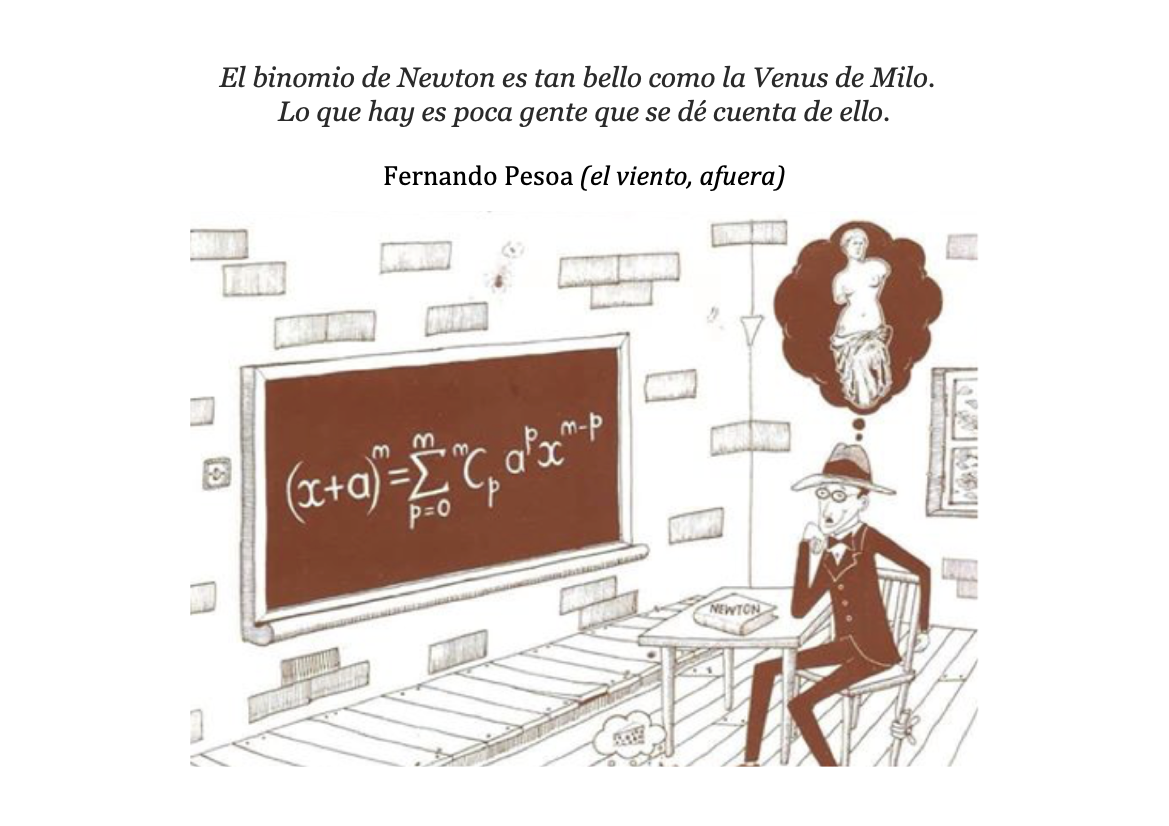
\includegraphics[width=0.85\textwidth]{img-reales/reales16.png}
	\end{figure}

\vspace{-10mm} %%%%%%%%%%%%%%%%%%%%%%
\begin{theorem}[ Propiedades del binomio de Newton]

\begin{enumerate}[1. ]
\item El término general del desarrollo es: $\ \ \mqty(n\\k)\, a^{n-k}\, b^k$

\textcolor{gris}{Si intercambianos $n-k$ por $k$, tenemos $\mqty(n\\n-k)\, a^k\, b^{n-k}\, . \ $ Los términos equidistantes del desarrollo tienen los mismos coeficientes.} 	

\item  Los coeficientes de $\, (a+b)^n \, $ son $\ \mqty(n\\0),\mqty(n\\1), \mqty(n\\2), \cdots , \mqty(n\\n)\, , \ $ coinciden con la fila $n$-sima del triangulo de tartaglia.

\item  La suma de los coeficientes del desarrollo de la potencia $n$-sima de un binomio es $\ 2^n$.

\textcolor{gris}{En efecto, si desarrollamos $(1+1)^n=2^n=\mqty(n\\0)+\mqty(n\\1)+\mqty(n\\2)+ \cdots + \mqty(n\\n)$}.

\end{enumerate}

\end{theorem}

	

\begin{miejercicio}

Calcular $(a-b)^4$

\rule{300pt}{0.1pt}

$(a-b)^4=[a+(-b)^4]$; los coeficientes serán los de la fila $4^a$ de Tartaglia, $\ 1,2,6,4,1$, así,

\vspace{2mm}$(a-b)^4=1a^4+4a^3(-b)+6a^2(-b)^2+4a(-b)^3+1(-b)^4=a^4-4a^3b+6a^2b^2-4ab^3+b^4$
	
\end{miejercicio}



\begin{miejercicio}

Calcula el término en $x^{12}$ del desarrollo de $(2x^2-1)^9$	

\rule{300pt}{0.1pt}

El término $k$-ésimo del desarrollo de $(a+b)^n$ es de la forma: $\  \mqty(n\\k) a^{n-k}b^k$

$(2x^2)^{9-k}2^{9-k}\, x^{2(9-k)} \ \to x^{18-2k}=x^{12} \ \to  18-2k=12 \ \to \ 6=2k \ \to \boldsymbol{k=3}$

Luego, el término buscado será:

$\mqty(9\\3)(2x^2)^{9-3}(-1)^3=\dfrac{9!}{3!\cdot 6!}(2x^2)^6(-1)=-\dfrac{9\cdot 8\cdot 7}{3\cdot 2} 2^6 x^{12} =-84\cdot 64x^{12}=\boldsymbol{ -5376x^{12} }$
\end{miejercicio}






\vspace{1cm}
\section{Ejercicios}
\begin{tikzpicture}
	\fill [left color=red!50, right color=teal!50] (0,0) rectangle (3.5,.1);
	\fill [left color=teal!50, right color=blue!50] (3.5,0) rectangle (7.5,.1);
	\end{tikzpicture}
\vspace{0.5cm}


\begin{mipropuesto}

Explica si estas frases son verdaderas o falsas:

\begin{enumerate}[a) ]
\item Hay números irracionales que son enteros.

\item Todo número irracional es real.

\item Todos los números decimales son racionales.

\item Entre dos números racionales hay infinitos números irracionales.

\item Todos los números decimales son racionales.

\item Entre dos enteros siempre hay un entero más.	
\end{enumerate}
\end{mipropuesto}

\vspace{-8mm}
\begin{flushright}
\begin{footnotesize} \textcolor{gris}{\rotatebox{180}{V: b, d}}	\end{footnotesize}
\end{flushright}


\begin{mipropuesto}

Escribe como intervalos:	 

\hspace{2cm} $a)\  \{x\in \mathbb R\, / \, -2\leq x \leq 3\}\,; \qquad b)\  \{x\in \mathbb R\, / \, -2< x \leq 3\}$

\hspace{2cm} $c)\  \{x\in \mathbb R\, / \, -2\leq x < 3\}\,; \qquad  d)\ \{x\in \mathbb R\, / \, -2< x < 3\}$

\hspace{2cm} $e)\  \{x\in \mathbb R\, / \,  x \leq 3\}\,; \quad \qquad \qquad  f)\ \{x\in \mathbb R\, / \,  x > -2 \}$
\end{mipropuesto}

\vspace{-8mm}
\begin{flushright}
\begin{footnotesize} \textcolor{gris}{\rotatebox{180}{ $\quad a)\ [-2,3]; \ \ b)\ ]-2,3]; \ \ c)\ [-2,3[; \ \ d)\ ]-2,3[; \ \ e)\ ]-\infty,3]; \ \ f)\ ]-2,+\infty[$ }}	\end{footnotesize}
\end{flushright}



\begin{mipropuesto}

Determina cuales son los números reales cuya distancia a $-1$ es menor que $2$.	
\end{mipropuesto}

\vspace{-8mm}
\begin{flushright}
\begin{footnotesize} \textcolor{gris}{\rotatebox{180}{$\{x\in \mathbb R \, / \, d(x,-1)<2\}\ = \ E_2(-1) \ \equiv \ ]-3,1[$}}	\end{footnotesize}
\end{flushright}

\begin{mipropuesto}

Introduce y extrae factores del radical.	

$\sqrt[3]{81\cdot 10^4\, x^6};\qquad \sqrt{\dfrac{16a^4}{27}} ;\qquad (x+1)\sqrt{\dfrac{x-1}{x+1}};\qquad \dfrac 2{x} \sqrt[3]{x^2} $
\end{mipropuesto}

\vspace{-8mm}
\begin{flushright}
\begin{footnotesize} \textcolor{gris}{\rotatebox{180}{$30x^2\sqrt{30};\qquad \dfrac{4a^2}{3\sqrt{3}};\qquad \sqrt{x^2-1};\qquad \sqrt[3]{\dfrac 8 x}$}}	\end{footnotesize}
\end{flushright}


\begin{mipropuesto}
	
	Calcula: $\quad \dfrac{8\sqrt{72}-3\sqrt{288}-2\sqrt{338}}{7\sqrt{2}} \qquad \qquad  -2\sqrt{\dfrac{20}{27}} +\sqrt{\dfrac{125}{3}}-\dfrac 6 5 \sqrt{\dfrac{45}{12}}-3 \sqrt{\dfrac 5 3}$
\end{mipropuesto}

\vspace{-8mm}
\begin{flushright}
\begin{footnotesize} \textcolor{gris}{\rotatebox{180}{$-2\, ; \qquad \qquad -\dfrac{17}{15}\sqrt{\dfrac{5}{3}}$}}	\end{footnotesize}
\end{flushright}


\begin{mipropuesto}
	
	Efectua las siguientes operaciones:
\begin{multicols}{2}	
	\begin{enumerate}[a) ]
	\item 	$\sqrt{\sqrt{a^2\cdot \sqrt[3]{a^2}}}$
	\item $\dfrac{\sqrt[3]{x^2y^2}\cdot \sqrt{xy}}{\sqrt[6]{x^11y^8}}$
	\item   $\sqrt[3]{(-1)^3\, \sqrt[5]{\sqrt[3]{-1}}}+1$
	\item $(1-2\sqrt{2})^2-(1+2\sqrt{2})^2$
	\item $(\sqrt{5}-2)\cdot (\sqrt{5}+2)+(2\sqrt{2})^2$
	\item $\sqrt{4+2\sqrt{3}}-\sqrt{4+2\sqrt{3}}\qquad (*)$
	\end{enumerate}
\end{multicols}
$f)\quad \sqrt{a^3-a^2b}+\sqrt{(a-b)(a^2-2ab+b^2)}+\sqrt{ab^2-b^3}$
\vspace{1mm}
\end{mipropuesto}



\vspace{-8mm}
\begin{flushright}
\begin{footnotesize} \textcolor{gris}{\rotatebox{180}{$a)\ \sqrt[3]{a};\quad b) \ \sqrt[6]{\dfrac{y^9}{x^4}};\quad c) \ 2;\quad d)\  -8\sqrt{2};\quad e)\  9;\quad f) \ 2a\sqrt{a-b}$}}	\end{footnotesize}
\end{flushright}

\vspace{-8mm}
\begin{flushright}
\begin{footnotesize} \textcolor{gris}{\rotatebox{180}{$e)\ (*)\ $ eleva, previamente, al cuadrado.}}	\end{footnotesize}
\end{flushright}

\begin{mipropuesto}
	
	Calcula: $\quad a)\ \ \dfrac{3}{\sqrt{3}-\sqrt{2}} - \dfrac{2}{\sqrt{3}+\sqrt{2}}\, ; \qquad\qquad b) \ \ \dfrac{\sqrt{7}-\sqrt{5}}{\sqrt{7}+\sqrt{5}}-\dfrac{\sqrt{7}+\sqrt{5}}{\sqrt{7}-\sqrt{5}}$

\end{mipropuesto}

\vspace{-8mm}
\begin{flushright}
\begin{footnotesize} \textcolor{gris}{\rotatebox{180}{$a)\ 3+5\sqrt{2}; \qquad b)\ -2\sqrt{35} $}}	\end{footnotesize}
\end{flushright}


\begin{mipropuesto}
	
	Racionaliza:
	
	\begin{multicols}{2}
	\begin{enumerate}[a) ]
	\item 	$\dfrac{1-\sqrt{3}}{2\sqrt{3}}$
	\item $\left( \dfrac{x^2}{\sqrt{x^3}} \right)^2$
	\item $\dfrac{\sqrt{x}+\sqrt{y}}{\sqrt{x}-\sqrt{y}}$
	\item $\dfrac{3+2\sqrt{5}}{2\sqrt{3}-\sqrt{6}}$
	\end{enumerate}
	\end{multicols}
	\vspace{1mm}
\end{mipropuesto}

\vspace{-8mm}
\begin{flushright}
\begin{footnotesize} \textcolor{gris}{\rotatebox{180}{$a)\ \dfrac{\sqrt{3}-6}{6};\qquad b)\ x;\qquad c)\ \dfrac{x+y+2\sqrt{xy}}{x-y};\qquad d)\ 2+\sqrt{2}+\sqrt{3}+ \dfrac {\sqrt{6}}{2} $}}	\end{footnotesize}
\end{flushright}

\begin{mipropuesto}
	
	Calcula:	
$\quad a)\ \dfrac{\sqrt
24-\sqrt{150}+4\sqrt{54}}{\sqrt{6}};\qquad \qquad \qquad b)\ \dfrac{\sqrt{3}}{2\sqrt{3}-2}-\dfrac{5}{\sqrt{3}+3}+\dfrac{2}{\sqrt
{3}}$
\end{mipropuesto}

\vspace{-8mm}
\begin{flushright}
\begin{footnotesize} \textcolor{gris}{\rotatebox{180}{$a)\ 9;\quad b) \dfrac{21}{12}(\sqrt{3}-1)$}}	\end{footnotesize}
\end{flushright}


\begin{mipropuesto}
	
	Calcula:
\begin{multicols}{2}	
\begin{enumerate}[a) ]
	\item $\log_2 0.25$
	\item $\mathrm{Log}\, 0.001$
	\item $\log_4 2$
	\item $\log_9 27$
	\item $\log_3 0.333\cdots$
	\item $\log_3 \dfrac{2}{54}$
	\item $\log_{0.01}100$
	\item $\log_{1/8} \dfrac 1 4$
\end{enumerate}
\end{multicols}	
\vspace{1mm}
\end{mipropuesto}

\vspace{-8mm}
\begin{flushright}
\begin{footnotesize} \textcolor{gris}{\rotatebox{180}{$a)\ -2;\quad b)\  -3;\quad c) 1/2;\quad d) \ 3/2;\quad e)\ -1;\quad f) -3;\quad g) -1;\quad h) \ -2/3$}}	\end{footnotesize}
\end{flushright}

\begin{mipropuesto}

Calcula: $\quad \log_6 x=2.5$	
\end{mipropuesto}

\vspace{-8mm}
\begin{flushright}
\begin{footnotesize} \textcolor{gris}{\rotatebox{180}{$36\sqrt{6}$}}	\end{footnotesize}
\end{flushright}

\begin{mipropuesto}
	
	Calcula:

\begin{multicols}{2}	
\begin{enumerate}[a) ]
	\item $\log_3 7\cdot \log_7 3$
	\item $-\log_3 5 \cdot \log_5 9$
	\item $\log_7(\log_3(\log_2 8)))$
	\item $\log_4(\log_2(\log_3(10-\mathrm{Log}\, 10)))$
\end{enumerate}
\end{multicols}
\vspace{1mm}	

\end{mipropuesto}

\vspace{-8mm}
\begin{flushright}
\begin{footnotesize} \textcolor{gris}{\rotatebox{180}{$a)\ 1;\qquad b)\ -2;\qquad c)\ 0;\qquad d)\ 0$}}	\end{footnotesize}
\end{flushright}

\vspace{-8mm}
\begin{flushright}
\begin{footnotesize} \textcolor{gris}{\rotatebox{180}{El cambio de base de los logaritmos puede serte útil.}}	\end{footnotesize}
\end{flushright}


\begin{mipropuesto}

Demuestra que: 
$\qquad a)\ \ \log_ba\, \log_db\, \log_ed=\log_ea\, ; \qquad b)\ \ \log_ba=\dfrac{1}{\log_ab}$ 	
\end{mipropuesto}

\vspace{-8mm}
\begin{flushright}
\begin{footnotesize} \textcolor{gris}{\rotatebox{180}{a) escribe toco con $\log_e$; $\qquad$  b) déjalo todo con $\log_a$.}}	\end{footnotesize}
\end{flushright}


\begin{mipropuesto}

$(x+1)^{\log(x+1)}=100(x+1)$	
\end{mipropuesto}

\vspace{-8mm}
\begin{flushright}
\begin{footnotesize} \textcolor{gris}{\rotatebox{180}{ Tomando logaritmos decimales se llega a una ecuación de segundo grado en $\log(x+1)$}}	\end{footnotesize}
\end{flushright}



\begin{mipropuesto}

?`Es cierta la siguiente igualdad? $\qquad \log(a^2-b^2)=\log(a\cdot b)+\log \left( \dfrac a b - \dfrac b a \right)$ 	
\end{mipropuesto}

\vspace{-8mm}
\begin{flushright}
\begin{footnotesize} \textcolor{gris}{\rotatebox{180}{ Basta con operar y aplicar propiedades de los logaritmos. }}	\end{footnotesize}
\end{flushright}

\begin{mipropuesto}
	
Calcula:

\vspace{2mm} $a) \ \dfrac{12(k-2)!}{k!}; \qquad b)\ \mqty(k\\k-2)=10;\qquad c)\ 3\mqty(k\\4)=5\mqty(k\\2);\qquad d) \ \dfrac{(k+6)!}{(k+4)!}=72$

\end{mipropuesto}


\vspace{-8mm}
\begin{flushright}
\begin{footnotesize} \textcolor{gris}{\rotatebox{180}{$a)\ 4;\qquad b)\ 5;\qquad c)\ 7;\qquad d)\ 3$}}	\end{footnotesize}
\end{flushright}


\begin{mipropuesto}
	
	Calcula el octavo término del desarrollo $\ (x^2-3y^3)^{10}$	

\end{mipropuesto}

\vspace{-8mm}
\begin{flushright}
\begin{footnotesize} \textcolor{gris}{\rotatebox{180}{El octavo término se alcanza con $k=7;\qquad -262440x^6y^{21}$}}	\end{footnotesize}
\end{flushright}



\begin{mipropuesto}
	
	Calcula el término independiente de $\ \left( a^3-\dfrac{2}{a} \right)^{20} $	

\end{mipropuesto}

\vspace{-8mm}
\begin{flushright}
\begin{footnotesize} \textcolor{gris}{\rotatebox{180}{El término independiente es $\ x^0;\qquad -208\, 035\, 0721$}}	\end{footnotesize}
\end{flushright}

\begin{mipropuesto}

Desarrolla: $\quad \left( \sqrt{\dfrac 2 x }+\sqrt{2x} \right)^2$	
\end{mipropuesto}

\vspace{-8mm}
\begin{flushright}
\begin{footnotesize} \textcolor{gris}{\rotatebox{180}{$16 \; x^{4} + 128 \; x^{3} + 448 \; x^{2} + 896 \; x^{1} + 1120 \; + 896 \; x^{-1} + 448 \; x^{-2} + 128 \; x^{-3} + 16 \; x^{-4}$}}	\end{footnotesize}
\end{flushright}









\newpage

\begin{adjustwidth}{50pt}{250pt}
\begin{cuadro-naranja}
\textbf{\huge{Problemas $\boldsymbol{+}$}}\normalsize{$\, $}
\end{cuadro-naranja}	
\end{adjustwidth}

\vspace{2mm}
\begin{enumerate}[\textbf{P$\boldsymbol +$} 1. ]
\item	?`Qué falla en la siguiente demostración?

\begin{multicols}{2}
\begin{enumerate}
\item $4=4$
\item $4\cdot(-5)=4\cdot(-5)$
\item $-20=-20$
\item $16-36=25-45$
\item $16-36+\dfrac {81} 4=25-45+\dfrac {81} 4$
\item $\left(4-\dfrac 9 2 \right)^2=\left(5-\dfrac 9 2 \right)^2$
\item $4-\dfrac 9 2 = 5-\dfrac 9 2$
\item $\boxed{ \ \boldsymbol{4\ = \ 5} \ } $ 

\QED
\end{enumerate}
\end{multicols}
\vspace{-6mm}
\begin{flushright}
\begin{footnotesize} \textcolor{gris}{\rotatebox{180}{En el paso f) a g) no se han tomado valores absolutos.}}	\end{footnotesize}
\end{flushright}

\item Calcula: $\quad a)\ 27^{\widehat{0.3}};\qquad b)\ \sqrt[3]{8^{27x^3}}$
\vspace{-6mm}
\begin{flushright}
\begin{footnotesize} \textcolor{gris}{\rotatebox{180}{Escribe como potencias de exponente racional. $\qquad a) \ 3;\quad b) \ 8^{9x^3} $ }}	\end{footnotesize}
\end{flushright}

\item Calcula: $\quad  a) \ \dfrac{\sqrt{2}+\sqrt{6}}{\sqrt{2+\sqrt{3}}} ;\qquad b)\  \sqrt{4+\sqrt{7}}-\sqrt{4-\sqrt{7}} ;\qquad c)\ \sqrt{4+\dfrac{\sqrt{63}}{2}}+\sqrt{4-\dfrac{\sqrt{63}}{2}}$ 

\vspace{-6mm}
\begin{flushright}
\begin{footnotesize} \textcolor{gris}{\rotatebox{180}{Eleva al cuadrado previamente. $\qquad a) \ 2;\quad b) \ 	\sqrt{2};\quad c)\ 3 $ }}	\end{footnotesize}
\end{flushright}

\item Sean $\ x=\dfrac{\sqrt{3}-\sqrt{2}}{\sqrt{3}+\sqrt{2}}  \ \ \text{ e } \ \ y=\dfrac{\sqrt{3}+\sqrt{2}}{\sqrt{3}-\sqrt{2}}\, , \  $  calcula $\ \ x^2+xy+y^2$

\vspace{-6mm}
\begin{flushright}
\begin{footnotesize} \textcolor{gris}{\rotatebox{180}{$99$ }}	\end{footnotesize}
\end{flushright}

\item Calcula $\ (log_2 3)\,(log_3 4)\,(log_3 5)\,(log_6 6)\, \cdot (log_{511} 512)$

\vspace{-6mm}
\begin{flushright}
\begin{footnotesize} \textcolor{gris}{\rotatebox{180}{Escríbelo todo como $\log_2\qquad $ sol.: 9 }}	\end{footnotesize}
\end{flushright}

\item Calcula $\ a)\ \text{ si } \ \log_2x=3 \ \to \ \text{ calcula }\ \log_x 64;\qquad \qquad b)\ 3\log_8 x=\log_4(x+6)$

\vspace{-6mm}
\begin{flushright}
\begin{footnotesize} \textcolor{gris}{\rotatebox{180}{Escríbelo todo como $\log_2\ \  $ sol.: $\ a)\ 2;\qquad  b)\ 3$ }}	\end{footnotesize}
\end{flushright}

\item Resuelve: $\quad a)\ 4^{\log_{16}{25}}=x;\qquad b)\ \log_{\log_3 9}8_x ;\qquad c)\ \ln{e^{\ln{(e^e)}}}=x$

\vspace{-6mm}
\begin{flushright}
\begin{footnotesize} \textcolor{gris}{\rotatebox{180}{Recuerda que $\ \log_a a^x=x=a^{\log_a x}\ \qquad \text{ sol.: }\  a)\ 25;\qquad b)\ 3;\qquad c)\ e$ }}	\end{footnotesize}
\end{flushright}

\item Calcula $\quad \log_2 x+\log_2 \sqrt{x} + \log_2 \sqrt{\sqrt{x}}+\log_2  \sqrt{\sqrt{\sqrt{x}}} +\, \cdots \, = \, 4 $

\vspace{-6mm}
\begin{flushright}
\begin{footnotesize} \textcolor{gris}{\rotatebox{180}{Recuerda la suma de infinitos términos de una progresión geométrica $\ \ [\, S_\infty=a_1/(1-r)\, ]\qquad $ sol.: $4$ }}	\end{footnotesize}
\end{flushright}

\item Prueba que $\ \dfrac{1}{\log_aabc}+\dfrac{1}{\log_babc}+\dfrac{1}{\log_cabc}=1$

\vspace{-6mm}
\begin{flushright}
\begin{footnotesize} \textcolor{gris}{\rotatebox{180}{ Escribe todos los logaritmos en la misma base. }}	\end{footnotesize}
\end{flushright}

\item Prueba que $\ \dfrac{1}{\log_\pi e}+\dfrac{1}{\log_e \pi}>2$

\vspace{-6mm}
\begin{flushright}
\begin{footnotesize} \textcolor{gris}{\rotatebox{180}{ solo tienes que escribir como cuadrado perfecto. }}	\end{footnotesize}
\end{flushright}

\vspace{-8mm}
\begin{flushright}
\begin{footnotesize} \textcolor{gris}{\rotatebox{180}{ Has de demostrar que $x+\dfrac 1 x >2$, con $x>0$, }}	\end{footnotesize}
\end{flushright}

\vspace{-8mm}
\begin{flushright}
\begin{footnotesize} \textcolor{gris}{\rotatebox{180}{ Escribe todos los logaritmos en la misma base. }}	\end{footnotesize}
\end{flushright}

\item Si el radio de una circunferencia de longitud  $\ \log b 4\ $ es $\ \log a^4\, , \ $ ?`Cuál es el valor de $\ \log_a b\, $?

\vspace{-6mm}
\begin{flushright}
\begin{footnotesize} \textcolor{gris}{\rotatebox{180}{ Longitud circunferencia = 2$\pi$ radio. \qquad sol: $\pi$}}	\end{footnotesize}
\end{flushright}

\item $\dfrac{1}{\log_2 a}+\dfrac{1}{\log_3 a}+\dfrac{1}{\log_4 a}=1\ $ ?`Cuál es el valor de $\ a\, $?

\vspace{-6mm}
\begin{flushright}
\begin{footnotesize} \textcolor{gris}{\rotatebox{180}{ Escribe todo en la misma base. $\qquad$ sol: $\ a=24$ }}	\end{footnotesize}
\end{flushright}

\item Calcula $\quad \dfrac{1}{\log_2(100!)}+\dfrac{1}{\log_3(100!)}+\dfrac{1}{\log_4(100!)}+\cdots +\dfrac{1}{\log_100(100!)}$

\vspace{-4mm}
\begin{flushright}
\begin{footnotesize} \textcolor{gris}{\rotatebox{180}{ Escribe todo en la misma base. $\qquad$ sol: $\ 1$ }}	\end{footnotesize}
\end{flushright}

\end{enumerate}

\newpage

\section{Resumen del tema}
\begin{tikzpicture}
	\fill [left color=red!50, right color=teal!50] (0,0) rectangle (3.5,.1);
	\fill [left color=teal!50, right color=blue!50] (3.5,0) rectangle (7.5,.1);
	\end{tikzpicture}
\vspace{0.5cm}

\begin{myblock}{ Resumen \emph{`Números reales'}}

\begin{figure}[H]
	\centering
	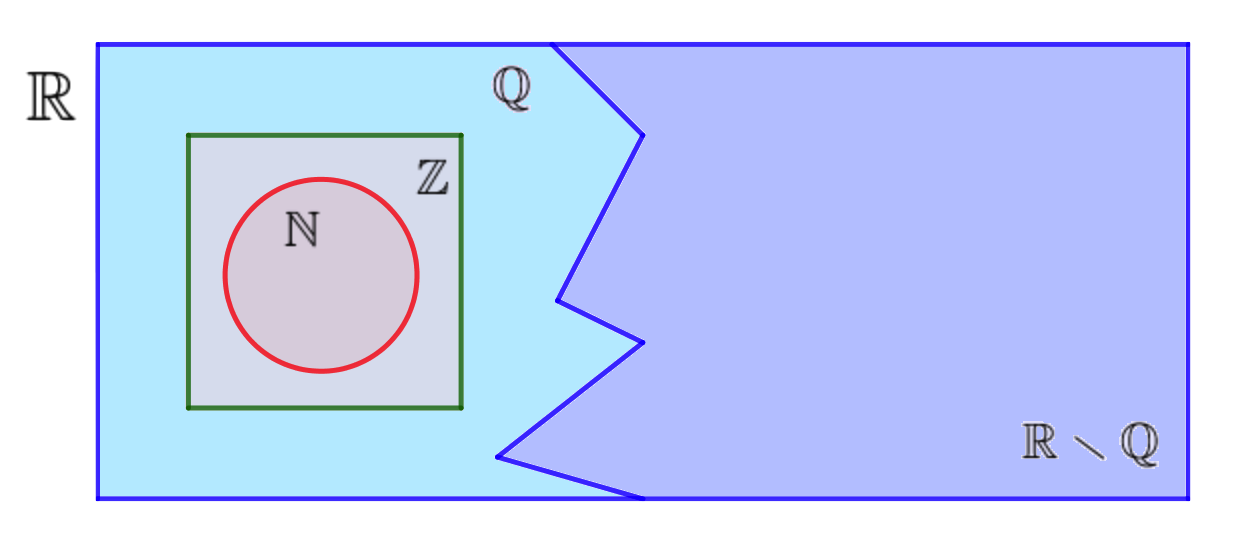
\includegraphics[width=0.75\textwidth]{img-reales/reales18.png}
	\end{figure}
	
\begin{table}[H]
\centering
\small
\begin{tabular}{|c|c|c|c|}
\hline
$|x|=\begin{cases} \  x & \text{ si } x\geq 0 \\  -x & \text{ si } x<0 \end{cases}$  & $[a,b[ \equiv \{\forall x \in \mathbb R \, / \, a\leq x < b \}$ & $d(x,y)=|x-y|$ & $E_r(a)=]a-r,a+r[$ \\ \hline
\end{tabular}
\end{table}

\vspace{5mm}
\begin{table}[H]
\centering
\begin{tabular}{|c|}
\hline
$\boldsymbol{ \sqrt[n]a \ = \ b \ \ \leftrightarrow \ \ b\ = \ a^n } \, ; \qquad a,b \in \mathbb R; \quad n\in \mathbb N\, , \ n>1$
 \\ \hline
\end{tabular}
\end{table}

\begin{table}[H]
\centering
\begin{tabular}{|c|c|c|}
\hline
$\sqrt[n]a^m=a^{m/n}$ & $\sqrt[n]{a} \, \cdot \, : \, \sqrt[n]{b} = \sqrt[n]{a\,  \cdot \, : \,  b}$ & $(\sqrt[n]{a})^m=\sqrt[n]{a^m}$ \\  \hline
$\sqrt[n]{\sqrt[m]{a}}=\sqrt[n\cdot m]{a}$ & $\sqrt[n]{a^m}=\sqrt[n\cdot k]{a^{m\cdot k}}$ & $b\sqrt[n]{a}=\sqrt[n]{b^n\, a}$ \\ \hline
\end{tabular}
\end{table}

\begin{table}[H]
\centering
\begin{tabular}{|c|c|c|}
\hline
Denominador & Factor racionalizante & Denominador racionalizado \\ \hline
$\sqrt[n]a^m$ & $\sqrt[n]a^{n-m}$ & $a$ \\ \hline
$\sqrt{a} \pm \sqrt{b}$ & $\sqrt{a} \mp \sqrt{b}$ & $a-b$ \\ \hline
\end{tabular}
\end{table}	

\vspace{5mm}

\begin{table}[H]
\centering
\begin{tabular}{|c|}
\hline
$\boldsymbol{ \log_aP\ = \ b \ \ \leftrightarrow \ \ a^P\ = \ b } \, ; \qquad a>0 \, \wedge \, a\neq 1 ;\quad P>0$
 \\ \hline
\end{tabular}
\end{table}

\begin{table}[H]
\centering
\begin{tabular}{|c|c|c|}
\hline
$\log_aa=1$ & $\log_a1=0$ & $\log_a(A\cdot B)=\log_aA+\log_aB$ \\ \hline
$\log_a(A / B)=\log_aA-\log_aB$ & $\log_aA^n=n\, \log_aA$ & $\log_bP=\dfrac{\log_aP}{\log_ab}$ \\ \hline
\end{tabular}
\end{table}	
\vspace{5mm}

\begin{table}[H]
\centering
\begin{tabular}{|c|}
\hline
  $(a+b)^n  = \mqty(n\\0)a^nb^0+\mqty(n\\1)a^{n-1}b^1+\mqty(n\\2)a^{n-2}b^2+ \cdots \mqty(n\\n-1)a^1b^{n-1}+\mqty(n\\n)a^0b^n $ \\ \hline
\end{tabular}
\end{table}
\end{myblock}












\begin{comment}	



%%%%%%%%%%%%%%%%%%%%%%%%%%%%%%%%%%%. SECCIONES
\chapter{texto}
\begin{tikzpicture}
	\fill [left color=red!50, right color=teal!50] (0,0) rectangle (6.5,.2);
	\fill [left color=teal!50, right color=blue!50] (6.5,0) rectangle (11.5,.2);
	\end{tikzpicture}

\vspace{1cm}
\section{texto}
\begin{tikzpicture}
	\fill [left color=red!50, right color=teal!50] (0,0) rectangle (3.5,.1);
	\fill [left color=teal!50, right color=blue!50] (3.5,0) rectangle (7.5,.1);
	\end{tikzpicture}
\vspace{0.5cm}

\subsection{texto}
\begin{tikzpicture}
	\fill [left color=red!50, right color=teal!50] (0,0) rectangle (3.5,.01);
	\fill [left color=teal!50, right color=blue!50] (3.5,0) rectangle (7.5,.01);
	\end{tikzpicture}
\vspace{0.5cm}


%$$$$$$$$$$$$$$$$$$$$$$$$$$$$$$$$$$$$$$$$$$$$$$$$$$$$$$$$$
\begin{mipropuesto}
	
	Calcula	

\end{mipropuesto}

\vspace{-8mm}
\begin{flushright}
\begin{footnotesize} \textcolor{gris}{\rotatebox{180}{E}}	\end{footnotesize}
\end{flushright}
%$$$$$$$$$$$$$$$$$$$$$$$$$$$$$$$$$$$$$$$$$$$$$$$$$$$$$$$$$

%%%%%%%%%%%%%%%%%%%%%%%%%%%%%%%%%%%. \begin{ ------>. 
detsacado;  cuadro-naranja;  cuadro-gris;  miejercicio (solución extensa);  mipropuesto (solución corta y fuera del cuadro)

%%%%%%%%%%%%%%%%%%%%%%%%%%%%%%%%%%%. CURIOSIDAD
\vspace{1cm}
\color{ForestGreen!80}
\rule{250pt}{0.2pt}
Texto
\vspace{-8mm}
\begin{flushright}
\rule{250pt}{0.2pt}		
\end{flushright}	
\color{black}
\end{comment} %A y A
\chapter{Sucesiones}
\begin{tikzpicture}
	\fill [left color=red!50, right color=teal!50] (0,0) rectangle (6.5,.2);
	\fill [left color=teal!50, right color=blue!50] (6.5,0) rectangle (11.5,.2);
	\end{tikzpicture}


\vspace{15mm}


\begin{adjustwidth}{40pt}{40pt}
\begin{cuadro-gris}

	\begin{multicols}{2}
	$\triangleright \quad$  Sucesiones. Término general.
	
	$\triangleright \quad$  Progresiones aritméticas y geométricas.
	
	$\triangleright \quad$  Monotonía y acotación.
	
	$\triangleright \quad$  Aproximación al concepto de límite de una sucesión.
	\end{multicols}
	
\end{cuadro-gris}
\end{adjustwidth}



\vspace{5mm}
\section{Sucesión. Término general}
\begin{tikzpicture}
	\fill [left color=red!50, right color=teal!50] (0,0) rectangle (3.5,.1);
	\fill [left color=teal!50, right color=blue!50] (3.5,0) rectangle (7.5,.1);
	\end{tikzpicture}
\vspace{0.5cm}

\begin{definition}[ Sucesión.]

Una sucesión es un conjunto ordenado de números reales :
                        $\  a_1, a_2, a_3, a_4, a_5, \cdots \equiv \{a_n\}$
                         
                         
\vspace{2mm} Se trata de funciones reales de variable natural: $\{a_n\}:\ \mathbb N \longrightarrow \mathbb R\, , $ la variable independiente es un número natural y la variable dependiente es un número real. 
                         
                         
\vspace{2mm} Las sucesiones se suelen representar por letras latinas minúsculas con el subíndice $n$ y encerradas entre llaves, $\{a_n\}$. A cada uno de los números que  la forman  se les llama \emph{término} de la sucesión y se designa por $a_i$, siendo  $i$  la posición o lugar dicho término ocupa  en la sucesión.
\end{definition}

\begin{miejemplo}


\begin{table}[H]
%\centering
\begin{tabular}{llll}
 & $\{a_n\}	\, :\ 1,3,5,7,9, \cdots$ &  & $\to \ a_3=\ 5$ \\
 & $\{b_n\}	\, :\ 2,4,8,16,32, \cdots$ &  & $\to \ b_5=32$ \\
 & $\{c_n\}	\, :\ 1,4,27,256, \cdots$ &  & $\to \ c_2=\ 4 $
\end{tabular}
\end{table}
\end{miejemplo}

\begin{definition}[ Término general.]

El término general de una sucesión es una expresión (fórmula) que nos permite calcular cualquier término de la sucesión sabiendo el lugar que ocupa, lo representamos por $a_n$.	

\vspace{2mm} Su utilidad es doble:

--- Permite calcular cualquier término de la sucesión sin más que saber el lugar que éste ocupa. Es por ello que el término general representa a toda la sucesión.

--- También es útil para averiguar si un numero dado es o no un término de la sucesión y, si lo es, averiguar la posición que ocupa.
\end{definition}

\begin{miejercicio}

Considerar la sucesión cuyo término general está definido por  $a_n=\dfrac{3n+2}{2n-1}	$

\begin{enumerate}[a) ]
\vspace{-2mm} \item Calcula los tres primeros términos y el undécimo.
\vspace{-3mm} \item Averigua si el número $53/33$ es o no un término de la sucesión.
\vspace{-3mm} \item Haz lo mismo para el número $26/25$
\end{enumerate}

\vspace{-4mm}
\rule{250pt}{0.1pt}
\vspace{5mm}

$\triangleright \ a)\qquad a_1=\dfrac{3(1)+2}{2(1)-1}=5;\ \ a_2=\dfrac{3(2)+2}{2(2)-1}=\dfrac 8 3 ;\ \ a_3=\dfrac{3(3)+2}{2(3)-1}=\dfrac{11}{5};\ \ a_11=\dfrac 5 3$

\vspace{2mm}$\triangleright \ b)\qquad \dfrac{3n+2}{2n-1}=\dfrac {53}{33} \to 99n+66=106n-53 \to 119=7n \to n=\dfrac{119}{7}=17 \in \mathbb N $

\vspace{2mm}Sí, efectivamente ${53}/{33}$ es un término de la sucesión $\{a_n\}$ (o, abusando del lenguaje, de la sucesión $a_n$). Además, se trata del término decimoséptimo, así, $a_{17}=55/33$

\vspace{2mm}$\triangleright \ c)\qquad \dfrac{3n+2}{2n-1}=\dfrac{26}{25} \to 75n+50=52n-26 \to 23n=24 \to n=\dfrac{24}{23} \notin \mathbb N$

\vspace{2mm}No, el número $26/25$ no es un término de la sucesión $a_n \, , \ (26/25 \notin a_n)$.

\end{miejercicio}

Decimos que una sucesión es \textbf{recurrente} o está definida por \emph{recurrencia} cuando cada término, a partir de uno dado, se obtiene en función de dos o más de sus  anteriores. En estos casos no siempre es sencillo encontrar el término general; p. e.: $\ \{a_n\}:\ \ 1, 2, 3, 0, 5, -2, 7, \cdots$

$\textcolor{gris}{a_1=1,\ a_2=2,\ a_3=3,\ a_n=a_{n-3}+a_{n-2}-a_{n-1};\ \forall n>3}$.

\vspace{5mm}
\begin{myexampleblock}{La sucesión de Fibonacci}

\vspace{2mm} \emph{Supongamos que un par de conejos recién nacidos, un macho y una hembra se colocan en el campo. Los conejos son fértiles a la edad de un mes, así que al final del segundo mes una hembra puede producir otro par de conejos. Supongamos que nuestros conejos nunca mueren, y que las hembras siempre producen un nuevo par (un macho y una hembra) cada mes, desde el segundo mes de vida. La pregunta que Fibonacci se hizo fue la siguiente, ?`cuántos pares de conejos tendremos en un año?}

\vspace{4mm} \small{\textsf{Este es el famoso problema de los conejos que Leonardo de Pisa (1170-1241), conocido como Fibonacci, plantea (entre otros problemas) en su libro “Liber Abaci” (1202).}}

\begin{figure}[H]
	\centering
	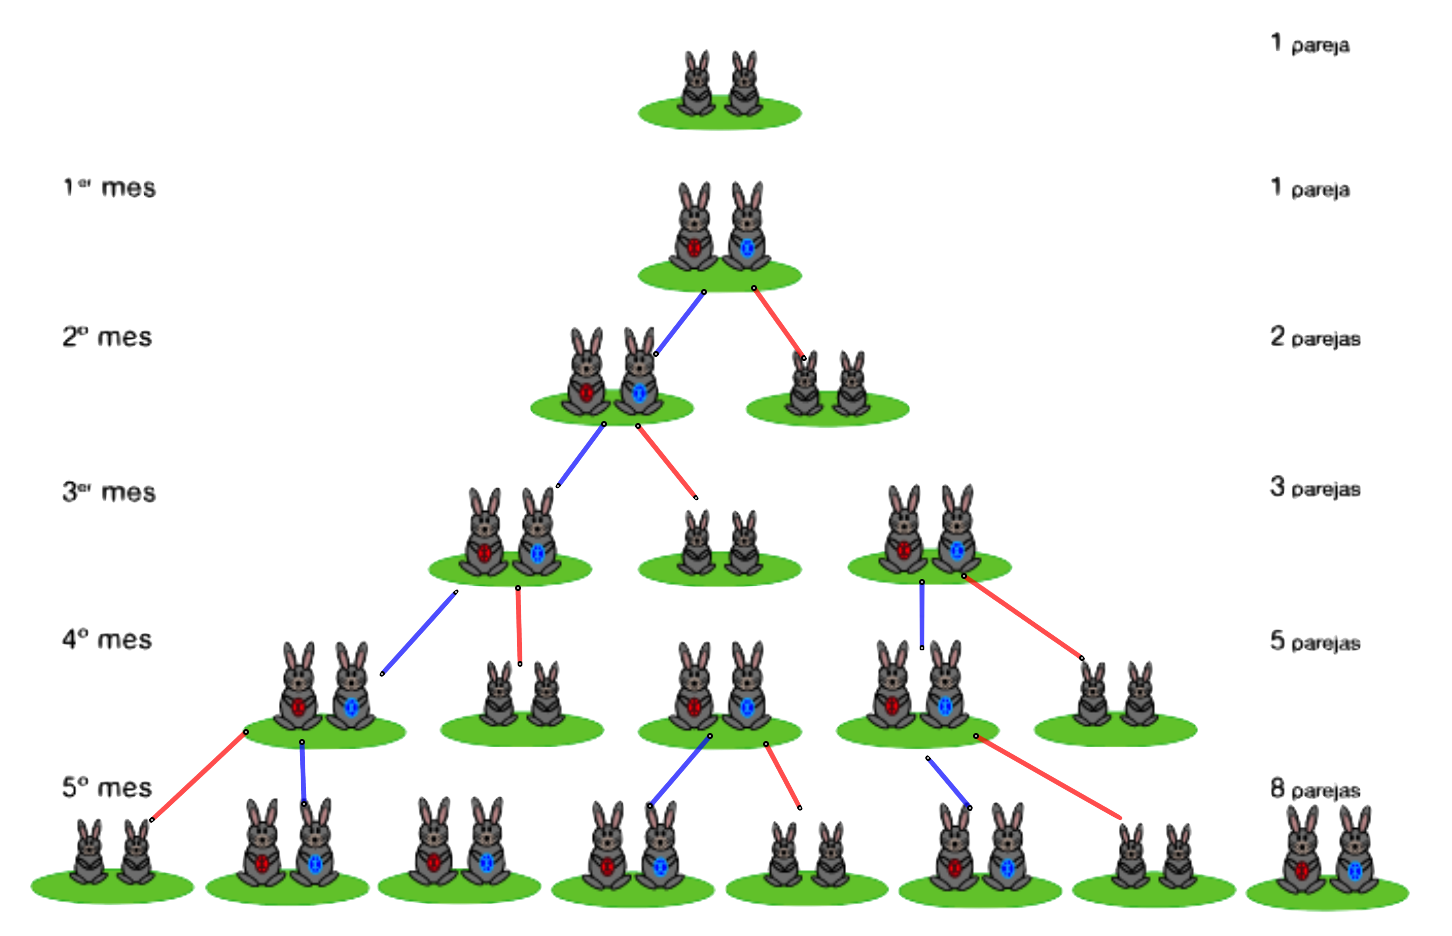
\includegraphics[width=0.9\textwidth]{img-suc/suc01.png}
	\caption*{\scriptsize{imagen : $\ $ https://oscarenfotos.com/2019/04/06/proporcion-aurea-y-fotografia/conejos\_fibonacci/}}
	\end{figure}
 
\vspace{2mm} Si observamos atentamente del enunciado del problema deducimos que:
\vspace{-1mm}
\begin{itemize}
	
\vspace{-2mm}\item Al final del primer mes, hay un solo par.

\vspace{-2mm}\item Al final del segundo mes, la hembra produce un nuevo par, así que ahora
tenemos dos parejas de conejos en el campo.

\vspace{-2mm}\item Al final del tercer mes, la hembra inicial produce un segundo par, haciendo que
en el campo tengamos tres pares de conejos.

\vspace{-2mm}\item Al final del cuarto mes, la hembra original ha producido otro nuevo par y la
hembra nacida dos meses antes produce su primer par, con lo que tendremos 5 pares.
\end{itemize}

\vspace{2mm} El número de pares de conejos en el campo al inicio de cada mes es:
$1, 1, 2, 3, 5, 8, 13, 21, 34, 55, 89, 144, \cdots$,
una sucesión, que se inicia con $1$ y $1$ donde cada nuevo término es la suma de los dos anteriores, y que recibe el nombre de \emph{sucesión de Fibonacci}: $\ \ \boldsymbol{ a_1=a_2=1;\ \ a_n=a_{n-1}+a_{n-2}\, , \ \forall n>2 }  \ \ (n\in \mathbb N)$ 

\vspace{2mm} Si hacemos el cociente de dos números consecutivos de la sucesión obtenemos esta otra:
$1/1=1, 2/1=2, 3/2=1.5, 5/3=1.666, 8/5=1.6, 13/8=1.625, 21/13=1.61538, \cdots$

\vspace{2mm} El cociente entre dos términos consecutivos de la sucesión tiende a un valor particular, el cual recibe el nombre de \emph{número de oro} o \emph{divina proporción} y tiene un valor aproximado de 1.61804, se representa por la letra griega phi, $\phi=\frac{1+\sqrt{5}}{2}$. 

\vspace{2mm}  La sucesión de Fibonacci tiene numerosas aplicaciones en ciencias de la computación, matemática y teoría de juegos. También aparece en configuraciones biológicas, como por ejemplo en las ramas de los árboles, en la disposición de las hojas en el tallo, en las flores de alcachofas y girasoles, en las inflorescencias del brécol romanesco, en la configuración de las piñas de las coníferas y en cómo el ADN codifica el crecimiento de formas orgánicas complejas. De igual manera, se encuentra en la estructura espiral del caparazón de algunos moluscos, como el nautilus.


\vspace{4mm} 
\begin{footnotesize}
Se puede encontrar su término general: $\ \ a_n=\dfrac 1{\sqrt{5}} \left[ \left(\dfrac{1+\sqrt{5}}{2}\right)^n-\left(\dfrac{1-\sqrt{5}}{2}\right)^n \right] =\dfrac{\phi^n-\phi^{-n}}{\sqrt{5}}=f_n$
\end{footnotesize}
\end{myexampleblock}


\begin{miejercicio}
. \normalsize{Determina} los cinco primeros términos de las sucesiones cuyos términos generales son:

\begin{multicols}{2}
$a_n=(-3)^n$

$b_n=3^{-n}$

$c_n=3n+1$

$d_n=\dfrac{n^2+1}{n^2}$

$e_n=n!-(n-1)!$

$\quad$

$\begin{cases} g_1=5 \\ g_2=-1\end{cases} \ \ g_n=g_{n-1}+2g_{n-
2},\, \forall n>2$	
\end{multicols}

\rule{250pt}{0.1pt}

\begin{multicols}{2}
\vspace{2mm} $\triangleright \ \ \{a_n\}:\ -3,\, 9,\, -27,\, 81,\, -243$

\vspace{2mm} $\triangleright \ \ \{b_n\}:\ 1/3,\ 1/9,\ 1/27,\ 1/81,\ 1/243$

\vspace{2mm} $\triangleright \ \ \{c_n\}:\ 4,\, 7,\, 10,\, 13,\, 16$

\vspace{2mm} $\triangleright \ \ \{d_n\}:\ 2,\, 5/4,\, 10/9,\, 17/16,\ 26/25$

\vspace{2mm} $\triangleright \ \ \{e_n\}:\ 0,\, 1,\ 4,\, 18,\, 96$

\vspace{2mm} $\triangleright \ \ \{g_n\}:\ 5,\, -1,\, 9,\, 7,\, 25$
\end{multicols}
	
\end{miejercicio}


\begin{miejercicio}

Encuentra, a ojo, el término general de las sucesiones cuyos primeros términos son:

\begin{multicols}{2}
	\vspace{2mm} $\triangleright \ \ \{a_n\}:\ 10,\, 20,\, 30,\, 40,\, \cdots$

\vspace{2mm} $\triangleright \ \ \{b_n\}:\ 2,\ 4,\ 6,\ 8,\ \cdots$

\vspace{2mm} $\triangleright \ \ \{c_n\}:\ 1,\, 3,\, 5,\, 7,\, \cdots$

\vspace{2mm} $\triangleright \ \ \{d_n\}:\ -1,\, 1,\, -1,\, 1,\ \cdots$

\vspace{2mm} $\triangleright \ \ \{e_n\}:\ 1,\, -4,\ 9,\, -16,\, \cdots$

\vspace{2mm} $\triangleright \ \ \{g_n\}:\ 7,\,7,\, 7,\, 7,\, \cdots$
\end{multicols}


\rule{250pt}{0.1pt}

\begin{multicols}{3}

\vspace{2mm}  $a_n=10n$

\vspace{2mm}  $b_n=2n$

\vspace{2mm}  $c_n=2n-1$

\vspace{2mm}  $d_n=(-1)^n$

\vspace{2mm}  $e_n=(-1)^{n+1} \ n^2$

\vspace{2mm}  $g_n=7$
	
\end{multicols}

\end{miejercicio}


\vspace{1cm}
\section{Progresiones aritméticas}
\begin{tikzpicture}
	\fill [left color=red!50, right color=teal!50] (0,0) rectangle (3.5,.1);
	\fill [left color=teal!50, right color=blue!50] (3.5,0) rectangle (7.5,.1);
	\end{tikzpicture}
\vspace{0.5cm}


\begin{definition}[ Progresión aritmética: PA]

Una progresión aritmética (PA) es una sucesión en la que cada término, salvo el primero, se obtiene sumando una cantidad constante al término anterior. Esta cantidad se llama \emph{distancia} o  diferencia de la progresión y se representa por $d$. Es por ello que si $\{a_n\}$ es una PA entonces queda unívocamente determinada al conocer $a_1$ y $d$.
\end{definition}


\vspace{4mm} Búsqueda del término general de una PA:
\begin{table}[H]
\centering
\begin{tabular}{ccccccccccc}
$a_1$ &  & $a_2$ &  & $a_3$ &  & $a_4$ & &$\cdots$ &  & $a_n$ \\
 & $+d$ &  & $+d$ &  & $+d$ & & $+d$ &  & $\cdots$ &   \\
$a_1$ &  & $a_1+d$ &  & $a_1+2d$ &  & $a_1+3d$ &  &$\cdots$ & & $a_1+(n-1)d$
\end{tabular}
\end{table}

\begin{definition}[ Término general de una PA]
. El término general de una progresión aritmética es :

$$\boxed{ \ 	\boldsymbol{ a_n  \ =  \  a_1 \, + \,   ( n - 1 )  \cdot  d } \ }$$
\end{definition}



\begin{miejercicio}

Encuentra el término general de las sucesiones cuyos primeros términos son:

$\{a_n\}:\ 13,15,17,19,\cdots \qquad  \qquad \{b_n\}:\ 11,7,3,-1,\cdots$

\rule{250pt}{0.1pt}
\vspace{2mm}
	
En la primera sucesión, cada término se obtiene del anterior al sumarle $d=2$ (las diferencias entre términos consecutivos es constante), se trata de un PA. Como el primer término es $a_1=13$, tenemos una $PA\begin{cases} \ a_1=13 \\ \ d=2 \end{cases}$.

\vspace{2mm} Su término general es:
$\quad a_n=13+(n-1)\cdot 2 \ \to \ \boldsymbol{a_n=2n+11}$

\vspace{4mm}

En la segunda sucesión, cada término se obtiene del anterior al sumarle $d=-4$ (las diferencias entre términos consecutivos es constante), se trata de un PA. Como el primer término es $b_1=11$, tenemos una $PA\begin{cases} \ b_1=11 \\ \ d=-4 \end{cases}$.

\vspace{2mm} Su término general es:
$\quad b_n=11+(n-1)\cdot (-4) \ \to \ \boldsymbol{b_n=-4n+15}$


\end{miejercicio}


\vspace{10mm}
\subsection{Suma de términos consecutivos de una progresión aritmética}
\begin{tikzpicture}
	\fill [left color=red!50, right color=teal!50] (0,0) rectangle (3.5,.01);
	\fill [left color=teal!50, right color=blue!50] (3.5,0) rectangle (7.5,.01);
	\end{tikzpicture}
\vspace{0.5cm}

\begin{large}\textbf{Interpolación de términos en una PA}\end{large}

\normalsize{Interpolar} $m$ medios aritméticos entre otros dos $a<b$ es encontrar una PA de $m+2$ términos de modo que $a, \, a_1,\ \cdots,\, a_m,\, b$ sea una PA. La distancia entre términos será (decimos que son medios porque están entre otros dos y aritméticos por tratarse de progresiones aritméticas):

$a_n=a_1+(n-1)d \ \to a_{m+2}=\boldsymbol b=a_1+[(m+2)-1] d= \boldsymbol{a+(m+1)d} \ \to \ \  \boldsymbol{ d=\dfrac{b-2}{m+1} }$

\vspace{5mm}\begin{large}\textbf{Suma de términos equidistantes en una PA}\end{large}

Los términos que equidistan de los extremos de una PA suman lo mismo que estos: 

$\text{Si } a_i,\, a_j \ \text{ son equidistantes en PA } \ \Rightarrow \ a_i+a_j=a_1+a_n$ 

\underline{Demostración}:

Los subíndices de los términos equidistantes han de ser tal que $i+j=n+1 \ \to j=n+1-i$

$a_i+a_j=a_i+a_{n+1-i}=a_1+(i-1)d+a_1+(n+1-i-1)d=a_1+(i-1)d+a_1+(n-i)d=2a_1+(i-1+n-i)d=2a_1+(n-1)d=a_1+a_1+(n-1)d=a_1+a_n$ \QED


\begin{myexampleblock}{Anécdota de Gauss}
\begin{multicols}{2}
\emph{``J. B. Büttner, maestro de un colegio alemán, castigó a todos los niños a sumar los 100 primeros números naturales para tenerlos entretenidos y callados un buen rato. Uno de los niños, Carl Friedrich Gauss obtuvo la respuesta casi de inmediato:  1 + 2 + 3 + … + 99 + 100  = 5050 .''}

\vspace{2mm} \emph{?`Cómo lo hizo?. Pues se dio cuenta de que la suma del primer número con el último (1+100) era igual que la del segundo número y el penúltimo (2+99), y así sucesivamente. Por lo que, como había cien números, se formaban 50 parejas con la misma suma, es decir 101. Por lo que sólo faltaba multiplicar 101 x 50 = 5.050.}

\begin{figure}[H]
	\centering
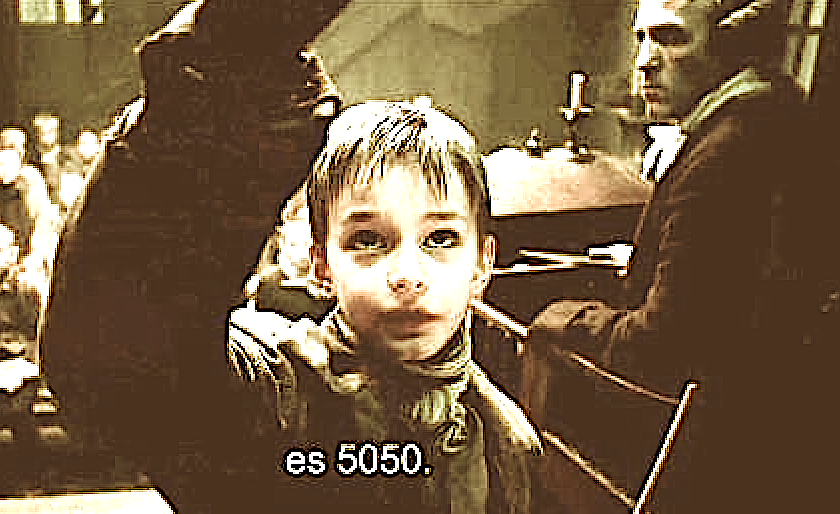
\includegraphics[width=0.4\textwidth]{img-suc/suc08.png}
	\end{figure}
\end{multicols}

\begin{small} \textsf{Johann Carl Friedrich Gauss (1777-1855) fue un niño prodigio que nació en una familia humilde y de padres analfabetos pero que fue autodidacta para aprender a leer y llegar a ser conocido como ``el príncipe de los matemáticos'' y reconocido por sus coetáneos como el ``matemático más grande desde la antigüedad''}.\end{small}
\end{myexampleblock}




\vspace{5mm}\begin{large}\textbf{Suma de los  $\boldsymbol n$  primeros términos de una PA}\end{large}

\vspace{3mm}
\begin{theorem}

La suma de $n$ términos consecutivos de una PA es igual a la semisuma de los extremos multiplicado por el número de términos.

$$\{a_n\}:\ PA \qquad a_1+a_2+a_3+\cdots + a_{n-1}+a_n= \displaystyle \sum_{k=1}^n	a_k = \ \boxed{ \boldsymbol{S_n\ = \ \ \dfrac{a_1+a_n}{2}\cdot n} \ }$$
\end{theorem}

\underline{Demostración}:

Disponiendo de derecha a izquierda la suma de términos y colocando debajo la misma en orden inverso y sumando, se observa que, en vertical, aparece $n$ veces la suma términos equidistantes, por la propiedad anterior, la suma de los extremos.

\begin{table}[H]
%\scriptsize
\centering
\begin{tabular}{c|cccccc}
$S_n \quad $ & $a_1$ & $a_2$ & $a_3$ & $\quad  \cdots \quad $ & $a_{n-1}$ & $a_n$ \\
$S_n \quad  $ & $a_n$ & $a_{n-1}$ & $a_{n-2}$ & $\cdots$ & $a_2$ & $a_1$ \\ \hline
$2\, S_n$ & $\quad a_1+a_n \quad $ & $a_2+a_{n-1}$ & $a_3+a_{n-2}$ & $\cdots$ & $a_{n-1}+a_2$ & $a_n+a_1$ \\ \hline
$2\, S_n$ & $\quad a_1+a_n \quad $ & $a_1+a_n$ & $a_1+a_n$ & $\cdots$ & $a_1+a_n$ & $a_1+a_n$
\end{tabular}
\end{table}

Luego $\quad 2S_n = n\, (a_1+a_n) \ \to \ \ S_n\ = \ \ \dfrac{a_1+a_n}{2}\cdot n$\QED

\vspace{5mm}

\begin{miejercicio}

Interpola tres términos aritméticos entre -12 y 8.

\rule{250pt}{0.1pt}
\vspace{2mm}

$a=-12;\ b=8;\ m=3 \quad \to \quad d=\dfrac{8-(-12)}{3+1}=\dfrac{20}{4}=5$

\vspace{2mm} Los términos buscados son: $\quad -2;\ \boldsymbol{-7, \ -2, \ 3}  ; \ 8$	

\vspace{2mm}\begin{small} \textcolor{gris}{De otro modo: $-12,x,y,z,8:\ PA \to 8=-12+(5-1)d \to d= 5:\ \  -2;\ \boldsymbol{-7, \ -2, \ 3}  ; \ 8 $} \end{small}
\end{miejercicio}

\begin{miejercicio}

\normalsize{Calcula} la suma de los 100 primeros números naturales:
$1+2+3+\cdots +99+100=?$
\rule{250pt}{0.1pt}	

Tenemos una PA cuyo primer término es $1$, el último $100$ (hay $100$ términos) y cuya distancia es $1$. Nos preguntan por la suma de todos ellos.

\vspace{2mm} $S_{100} =\  \textcolor{gris}{S_n=\dfrac{a_1+a_n}{2}\, n} \ = \dfrac{1+100}{2}\, 100= 50.5\cdot 100=\ 5050 \quad $ \textcolor{gris}{(Problema de Gauss)}
\end{miejercicio}


\begin{miejercicio}

Calcula la suma de todos los múltiplos de $7$ comprendidos entre $250$ y $500$.

\rule{250pt}{0.1pt}
\vspace{2mm}

Los múltiplos de siete, $\dot{7}$, son números de la forma $7k,\ \forall k\in \mathbb N$. Forman una PA ya que pasa pasar de un múltiplo de $7$ al siguiente hay que sumarle $7:\ \ a_n=a_1+(n-1)\, 7$

\vspace{2mm}--- Búsqueda del primer término: $\ 7k=250 \to k=35.71\cdots \to 7\cdot 35=245 \to 245+7=\boldsymbol{252=a_1}\ $ Primer $\dot{7}$ en $[250,500]$.

\vspace{2mm}--- Búsqueda del último término: $\ 7k=500 \to k=71.42\cdot \to 7\cdot 71=\boldsymbol{497=a_n}\ $ Último $\dot{7}$ en $[250,500]$.

\vspace{2mm}--- Búsqueda del número de términos: $\ PA:\ a_1=252;\ d=7 \ \to a_n=a_1+(n-1)d\, : \ a_n=497=252+7(n-1) \to n-1=\dfrac{497-252}{7}=35 \to \boldsymbol{n=36}\ $ Hay un total de $36$ términos $\dot{7}$ en $[250,500]$. 

\vspace{2mm}Tenemos que sumar los $n=36$ términos de una PA en que $a_1=252$ y $a_n=497$, aplicando la fórmula:

\vspace{2mm} $S_{36} =\  \textcolor{gris}{S_n=\dfrac{a_1+a_n}{2}\, n} \ = \dfrac{252+497}{2}\, 36= \ 13482$

\end{miejercicio}


\vspace{5mm}

\begin{myalertblock}{Progresiones aritméticas de segundo orden}

\vspace{2mm} Una \emph{progresión aritmética de segundo orden} es una sucesión cuyo término general es un polinomio de segundo grado en $n:\quad a_n=An^2+Bn+C\, , \ n\in \mathbb N;\ \ A,B,C \, \text{constantes}$.
	
\vspace{2mm} La diferencia entre términos consecutivos no es ahora constante, es una PA (de primer orden). Lo que sí será constante (y caracterizará a este tipo de sucesiones) son las segundas diferencias.

\begin{table}[H]
\centering
\small
\begin{tabular}{lcccccccccc}
Progresión aritmética $\ a_n$ & $\quad$ & $\boldsymbol{a_1}$ &  & $a_2$ &  & $a_3$ &  & $a_4$ & $\cdots$ & $a_n$ \\
Primeras diferencias (PA) & &  & $\overrightarrow{\boldsymbol{ \ \ d_1 \ \ }}$ &  & $\overrightarrow{\ \ d_2 \ \ }$ &  & $\overrightarrow{\ \ d_3\ \ }$ &  & $\cdots$ &  \\
Segundas diferencias (cte) & &  &  & $\overrightarrow{\boldsymbol{\ \ d \ \ }}$ &  & $\overrightarrow{ \ \ d \ \ }$ &  & $\cdots$ &  & 
\end{tabular}
\end{table}

\vspace{2mm} Comprobémoslo: 

\vspace{2mm} $d_n=a_{n+1}-a_n=A(n+1)^2+B(n+1)+C-An^2-Bn-C=\cdots = (A+B)+(2A)\, n$

\vspace{2mm} $d_n$ es una progresión aritmética de primer término $A+B$ y distancia $2A$
 	

\vspace{2mm} \textcolor{gris}{Las segundas diferencias sí son una constante. Evidentemente, $\ d_{n+1}-d_n=A+B+2A\, (n+1) \, - \, A-B-2A\, n =2A=cte$ \QED}

\begin{table}[H]
\centering
\begin{tabular}{l|l|l|l|l|l}
$\boldsymbol{a_1}$ & $\boldsymbol{a_2}$ & $\boldsymbol{a_3}$ & $\boldsymbol{a_4}$ & $\boldsymbol{\cdots}$ & $\boldsymbol{a_n}$ \\ \hline
 & $a_1+d_1$ & $a_2+d_2$  & $a_3+d_3$ & $\cdots$ & $a_{n-1}+d_{n-1}$ \\
 & $a_1+d_1$ & $a_1+d_1+d_2$ & $a_1+d_1+d_2+d_3$ & $\cdots$ & $a_1+d_1+d_2+\cdots + d_{n-1}$
\end{tabular}
\end{table}	

\vspace{2mm} El término general de $a_n$ será:

\vspace{2mm} $a_n=a_1+d_1+d_2+\cdots +d_{n-1}=a_1+ S_{n-1}\textcolor{gris}{ [PG\{d_n\}] } =a_1+\dfrac{d_1+d_{n-1}}{2}\, (n-1)= a_1+\dfrac{d_1\, + \, d_1+([(n-1)-1]\, d}{2}\,(n-1)= a_1+\dfrac{d_1+d_1+(n-2)d}{2}(n-1)=a_1+\left[ d_1+\dfrac{n-2}{2}d\right](n-1)= a_1+d_1(n-1)+\dfrac{(n-1)(n-2)}{2}d$

\vspace{2mm} Dada una progresión aritmética de segundo orden (las segundas diferencias son constantes) nos fijamos en el primer término, 
$\boldsymbol{a_1}$, 
en la primera de sus primeras diferencias, 
$\boldsymbol{d_1}$ 
y en sus segundas diferencias (ctes), 
$\boldsymbol{d}$. 
El término general en función de estos tres datos es:

$$\subrayado{ \boxed{ \ \boldsymbol{ a_n \ = \ a_1+d_1\, (n-1)+\dfrac{(n-1)(n-2)}{2}\, d }\ } }$$

\vspace{5mm}

\rule{250pt}{0.1pt}

\vspace{2mm} \underline{Ejemplo 1}: Encuentra el término general de la sucesión $\ 1,6,13,22,33,\cdots $

\vspace{2mm} Las primeras diferencias son $5,7,9,11,\cdots$, que forman una PA. Las segundas diferencias son $2,2,2,\cdots$, siempre es una constante. Estamos ante una PA de segundo orden.

\vspace{2mm} En nuestro caso, llamando $a_n$ a la sucesión de partida, el primero de sus términos es $a_1=1$, la primera de sus primeras diferencias es $d_1=5$ y las segundas diferencias son todas $d=2$. Aplicando la fórmula anterior,
	
\vspace{2mm} $a_n=1+5(n-1)+\dfrac{(n-1)(n-2)}{2}2=1+5(n-1)+(n-1)(n-2)=n^2+2n+2$

\vspace{2mm} \textcolor{gris}{Comprobación: $\ a_1=1^2+2\cdot 1-2=1;\ a_2=2^2+2\cdot 2-2=6;\   a_3=3^2+2\cdot 3-2=13;\ \cdots $}

\vspace{2mm}

\begin{flushright} \rule{250pt}{0.1pt} \end{flushright}
 

\vspace{2mm} Es evidente comprobar que la sucesión de los cuadrados de una PA es una progresión aritmética de segundo grado.

\vspace{4mm} Se puede demostrar que la suma de $n$ términos consecutivos de una PA de segundo grado $a_n$ es:
$\quad S_n(\text{PA } 2^o \text{ grado}) \ = \ a_1\, n + d_1\, \dfrac{n(n-1)}{2}+d\, \dfrac{(n-2)(n-1)n}{6}$

\vspace{5mm}

\rule{250pt}{0.1pt}

\vspace{2mm} \underline{Ejemplo 2}: 

\vspace{2mm} La suma de $20$ términos de la sucesión $1+6+13+23+33+\cdots$ es:

\vspace{2mm} Del ejemplo anterior: $\quad a_1=1;\ d_1=5;\ d=2;\ n=20 \ \to \ S_{20}=3250$

\begin{flushright} \rule{250pt}{0.1pt} \end{flushright}


\end{myalertblock}


\vspace{1cm}
\section{Progresiones geométricas}
\begin{tikzpicture}
	\fill [left color=red!50, right color=teal!50] (0,0) rectangle (3.5,.1);
	\fill [left color=teal!50, right color=blue!50] (3.5,0) rectangle (7.5,.1);
	\end{tikzpicture}
\vspace{0.5cm}


\begin{definition}[ Progresión aritmética]

Una progresión geométrica (PG) es una sucesión en la que cada término, salvo el primero, se obtiene multiplicando por una cantidad constante al término anterior. Esta cantidad se llama \emph{razón} de la progresión y se representa por $r$. Es por ello que si $\{a_n\}$ es una PG entonces queda unívocamente determinada al conocer $a_1$ y $r$.
	
\end{definition}

\vspace{4mm} Búsqueda del término general de una PA:
\begin{table}[H]
\centering
\begin{tabular}{ccccccccccc}
$a_1$ &  & $a_2$ &  & $a_3$ &  & $a_4$ & &$\cdots$ &  & $a_n$ \\
 & $\times r$ &  & $\times r$ &  & $\times r$ & & $\times r$ &  & $\cdots$ &   \\
$a_1$ &  & $a_1\cdot r$ &  & $a_1 \cdot r^2$ &  & $a_1 \cdot r^3$ &  &$\cdots$ & & $a_1 \cdot r^{n-1}$
\end{tabular}
\end{table}

\begin{definition}[ Término general de una PG]

El término general de una progresión aritmética es: 
$\qquad \boxed{ \ 	\boldsymbol{ a_n  \ =  \  a_1 \, \cdot \,   r^{ n - 1 }   } \ }$	
\end{definition}


\begin{miejercicio}
	. Encuentra el término general de las sucesiones:

\vspace{2mm} $\{a_n\}:\ 3, -12 , 48, -192 , 768 , -3072, \cdots  \qquad  \qquad \{b_n\}:\  8, 4, 2, 1 , 1/2 , 1/4 , \cdots$
	
\rule{250pt}{0.1pt}

\vspace{2mm}
$\triangleright \ \ \{a_n\}\ $ es una PG cuyo primer término es $a_1=3$ y la razón $r=-4$, por lo que 

\vspace{2mm} $\ a_n=3\cdot (-4)^{n-1}$

\vspace{5mm}
$\triangleright \ \ \{b_n\}\ $ es una PG cuyo primer término es $b_1=8$ y la razón $r=1/2$, por lo que 

\vspace{2mm} $\ b_n=8\cdot (1/2)^{n-1}=\dfrac{2^3}{2^{n-1}}=2^{4-n}$

\end{miejercicio}

\vspace{5mm}
\subsection{Suma y producto de términos consecutivos de una progresión geométrica}
\begin{tikzpicture}
	\fill [left color=red!50, right color=teal!50] (0,0) rectangle (3.5,.01);
	\fill [left color=teal!50, right color=blue!50] (3.5,0) rectangle (7.5,.01);
	\end{tikzpicture}
\vspace{0.5cm}


\vspace{5mm}\begin{large}\textbf{Interpolación de términos en una PA}\end{large}

Interpolar $m$ medios geométricos entre otros dos $a<b$ es encontrar una PG de $m+2$ términos de modo que  $ \ a, \, a_1, \, \cdots ,\,  a_m,\ b$ sea una PG. La razón entre términos será (decimos que son medios porque están entre otros dos y geométricos por tratarse de progresiones geométricas):

$a_n=a_1\,  r^{n-1} \ \to a_{m+2}=\boldsymbol b=a\, r^{(m+2)-1} = 	\boldsymbol{a\, r^{m+1}} \ \to \ \  \boldsymbol{ r=\sqrt[m-1]{\dfrac{b}{a}} }$

\vspace{5mm}

\begin{large} \textbf{Suma de términos consecutivos de una progresión geométrica} \end{large}
\vspace{2mm}

\begin{theorem}

La suma de $n$ términos consecutivos de una PG es:

$$\{a_n\}:\ PG \qquad a_1+a_2+a_3+\cdots + a_{n-1}+a_n= \displaystyle \sum_{k=1}^n	a_k = \ \boxed{ \boldsymbol{S_n\ = \ \ \dfrac{a_n\, r-a_1}{r-1} \ } }$$

\end{theorem}

\underline{Demostración}:

\begin{table}[H]
\centering
\begin{tabular}{lllllll}
$\ S_n \ = \ $ & $a_1$ & $+a_2$  & $+a_3$ & $+ \ \cdots$  & $+a_{n-1}$ & $+a_n$ \\ \hline
$r\cdot S_n=$ & $r\cdot a_1$ & $+r\cdot a_2$  & $+r\cdot a_3$ & $+ \ \cdots$  & $+r\cdot a_{n-1}$ & $+r\cdot a_n$ \\
 & $a_2$ & $+a_3$ & $+a_4$ & $+\ \cdots$ & $+a_n$ & $+r\cdot a_n$ 
\end{tabular}
\end{table}

Restando: $r\cdot S_n-S_n= a_2 +a_3+a_4+\ \cdots+a_n+r\cdot a_n- 
a_1-a_2-a_3- \ \cdots-a_{n-1}-a_n =a_n\, r-a_1$

\vspace{2mm} Despejando: $\quad S_n=\dfrac{a_n\, r-a_1}{r-1}$ \QED

\vspace{0.5cm}

\begin{large} \textbf{Producto de términos consecutivos de una progresión geométrica} \end{large}
\vspace{3mm}

Para ello utilizaremos la siguiente propiedad:

\emph{El producto de términos equidistantes de una PG es igual al producto de sus extremos}, 

$\text{si } a_i,a_j \text{ son términos equidistantes de una PG } \ \Rightarrow \  \boldsymbol{a_i\cdot a_j = a_1\cdot a_n}$


\underline{demostración}: 

$a_i, \, a_j\ $ son términos equidistantes de una PG si $i+j=n+1 \ \to \ j=n+1-i$

$a_i\cdot a_j=a_i\cdot a_{n+1-i}=a_1\, r^{i-1} \cdot a_1\, r^{n+1-i-1}=a_1\ a_1\ r^{i-1\, + \ n+1-i-1}=a_1\, a_1 \, r^{n-1}=a_1\cdot a_n$ \QED

\vspace{0.5cm}

\begin{theorem}

El producto de $n$ términos consecutivos de una PG es:

$$a_1 \cdot a_2 \cdot \cdots \cdot a_n= \displaystyle \prod_{k=1}^n a_k  = \ 
\boxed{ \ \boldsymbol{   
P_n \ = \ \sqrt{ (a_1\cdot a_n)^n } 
} \ }$$	

\end{theorem}

\underline{Demostración}:

\begin{table}[H]
\centering
\begin{tabular}{l|lllll}
$P_n=$ & $a_1\cdot$ & $a_2\cdot$ & $\cdots \cdot$ & $a_{n-1}\cdot$  & $a_n$ \\
$P_n=$ & $a_n\cdot$ & $a_{n-1}\cdot$ & $\cdots \cdot$ & $a_2\cdot$ & $a_1$  \\ \hline
$P_n^2=$ & $(a_1\cdot a_n)$ & $(a_2\cdot a_{n-1})$ & $\cdots$ & $(a_{n-1}\cdot a_2)$  & $(a_n \cdot a_1)$ \\
  & $(a_1\cdot a_n)$  & $(a_1\cdot a_n)$  & $\cdots $  & $(a_1\cdot a_n)$  & $(a_1\cdot a_n)$ 
\end{tabular}
\end{table}

Luego, $\quad P_n^2=(a_1\cdot a_n)^n \quad \to \quad  P_n=\sqrt{(a_1\cdot a_n)^n}$ \QED

\vspace{5mm}

\begin{miejercicio}

Considera la sucesión: $\quad 2,4,8,16,\cdots$

$\quad$ a) Calcula el término general.

$\quad$ b) Calcula la suma de los diez primeros términos.

$\quad$ c) Calcula el producto de los cinco primeros términos.

\rule{250pt}{0.1pt}
\vspace{2mm}

$a)\quad $ Se trata de una $PG \ \begin{cases} \ a_1=2\\\ r=2 \end{cases} \to \ a_n=a_1\cdot r^{n-1}=2\cdot 2^{n-1}=2^n$

\vspace{2mm} $b)\quad a_{10}=2^{10}=1024 \quad \to \quad S_{10}=\dfrac{a_{10}\cdot r-a_1}{r-1}=\dfrac{1024\cdot 2-2}{2-1}=2046$

\vspace{2mm} $c)\quad a_5=2^5=32 \quad \to \quad P_5=\sqrt{(a_1\cdot a_5)^5}=\sqrt{(2\cdot 32)^5}=32768$
	
\end{miejercicio}

\begin{miejercicio}

Interpola 4 medios geométricos entre 1 y 243	.

\rule{250pt}{0.1pt}
\vspace{2mm}

$1, a_1, a_2, a_3, a_4, 243:\ PG \ \quad 243=1\, r^{6-1} \ \Rightarrow \ \  r=\sqrt[5]{\dfrac {243}{1}}=3 \to \, : \quad 1,\ \boldsymbol{3,\, 9,\, 27,\ 81,\ } 243$
\end{miejercicio}



\subsection{Suma de todos los términos de una progresión geométrica}
\begin{tikzpicture}
	\fill [left color=red!50, right color=teal!50] (0,0) rectangle (3.5,.01);
	\fill [left color=teal!50, right color=blue!50] (3.5,0) rectangle (7.5,.01);
	\end{tikzpicture}
\vspace{0.5cm}

\begin{theorem}[ Suma de los infinitos términos de una PG]

La suma de todos (infinitos) términos de una PG se puede efectuar siempre que la razón sea, en valor absoluto, menor que la unidad y vale:

$$\boldsymbol{ S_\infty \ = \ \dfrac{a_1}{1-r} } \qquad \qquad \text{siempre que } \ |r|<1$$
	
\end{theorem}


\underline{Demostración}:

Nos basamos en el hecho de que las sucesivas potencias de un número que, en valor absoluto, sea menor que la unidad se acercan cada vez más a cero a medida que aumenta el índice de la potencia, p.e.: $0.1^2=0.01;\ 0.1^{10}=0.0000000001;\ $ etc. Abusando del lenguaje podemos escribir que $r^\infty =0$, siempre que $|r|<1$

Así, $\ \ S_\infty=\dfrac{a_{\infty}r-a_1}{r-1}=\dfrac{a_1\cancelto{0}{r^\infty}-a_1}{r-1}=\dfrac{-a_1}{r-1}=\dfrac{a_1}{1-r}$ \QED

\begin{miejercicio}

Calcula la suma de todos los términos de la sucesión: $\ \dfrac 1 2, \, \dfrac 1 4, \, \dfrac 18, \, \cdots$	


\rule{250pt}{0.1pt}
\vspace{2mm} 

\begin{multicols}{2}
Tenemos una $PG \ \begin{cases} \ a_1=1/2 \\ \ r=1/2 \end{cases}$

$\qquad \text{como } |r|=1/2<1 \quad \to$

$\qquad \to  \quad S_\infty=\dfrac{1/2}{1-1/2}=1$


En la figura siguiente se muestra una \emph{demostración visual}.

\begin{figure}[H]
	\centering
	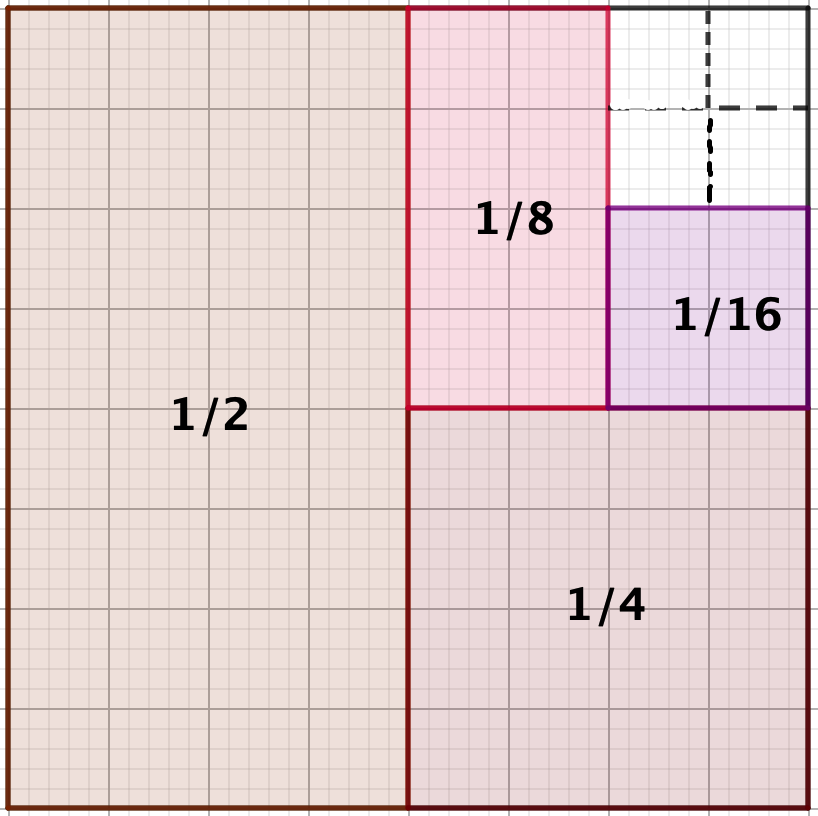
\includegraphics[width=0.25\textwidth]{img-suc/suc03.png}
\end{figure}
\end{multicols}
\end{miejercicio}
\vspace{1.5cm}%%%%%%%%%%%%%%%%%%%%%%%%%%
\begin{miejercicio}

Lanzamos una pelota a lo largo de un pasillo. En cada bote la pelota avanza una distancia igual a la mitad de la distancia anterior. Si al octavo bote se para, ¿qué distancia ha recorrido si antes del primer bote ha avanzado 2 m? Si no parase de botar, ¿sería necesario un pasillo infinito?

\rule{250pt}{0.1pt}
\vspace{2mm} 

$a_1=2,\, a_2=1,\, a_3=1/2,\, a_4=1/4,\,  \cdots \ :\ \ PG \to a_n=2\, \left(\dfrac 1 2\right)^{n-1}=2^{2-n} \ \Rightarrow \ a_8=\dfrac 1{64}$

\vspace{2mm} $S_8=\dfrac{a_8\cdot r -a_1}{r -1 }=\dfrac{\dfrac 1{64} \, \dfrac 1 2-2 }{1/2-1} \approx 3.98 \,  $m. $\ $ Distancia total recorrida en 8 botes

\vspace{4mm} Salto de $\infty$ botes: $\ \ S_\infty=\dfrac{a_1}{1-r}=\dfrac{2}{1-1/2}=4\, $m. $\ \ $ Distancia total recorrida tras $\infty$ botes, obviamente, no necesitamos un pasillo infinito.

	
\end{miejercicio}

 
\vspace{1.5cm}%%%%%%%%%%%%%%%%%%%%%%%%%%
\begin{figure}[H]
	\centering
	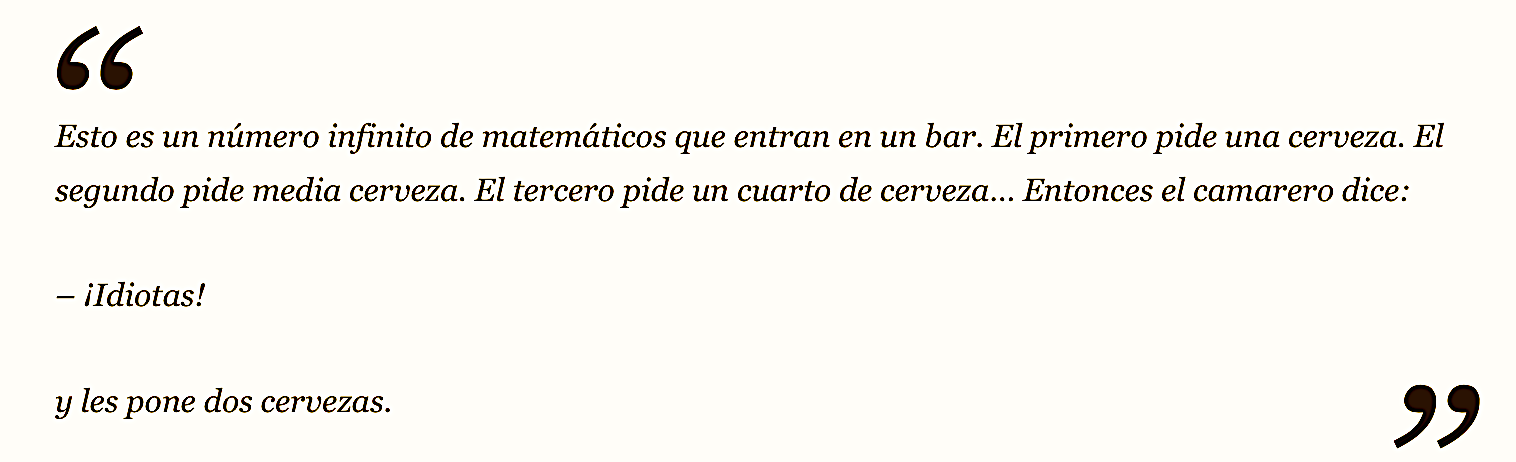
\includegraphics[width=0.95\textwidth]{img-suc/suc09.png}
\end{figure}
\vspace{1.5cm}%%%%%%%%%%%%%%%%%%%%%%%%%%

\vspace{15mm}
\begin{myalertblock}{Progresiones aritmético-geométricas}

\vspace{2mm} Si $a_n$ es una progresión aritmética y $b_n$ es una progresión geométrica, diremos que la sucesión $c_n= a_n \cdot b_n$, de términos $a_1 \cdot b_1,\,  a_2 \cdot  b_2,\,  a_3 \cdot b_3,\, \cdots ,\  $ es una \emph{progresión aritmético-geométrica}.

\vspace{2mm} Está claro que el término general de estas progresiones aritmético-geométricas siempre se puede expresar como  producto de los dos términos generales. Es decir, siempre podremos expresar su término general como $\quad \boldsymbol{c_n=(a\, n+b)\cdot r^n}\, , \quad a\neq 0, \ r\neq 0, \ r\neq 1$


\vspace{2mm} Cálculo de la suma de los $n$ primeros términos:

\vspace{2mm} $S_n=(a+b)r+(2a+b)r^2+(3a+b)r^3+\cdots+(na+b)r^n$

\vspace{2mm} $S_n=ar+2ar^2+3ar^3+\cdots + nar^n\ + \ br+br^2+\cdots br^n$

\vspace{2mm} $rS_n=ar^2+2ar^3+\cdots + nar^{n+1}\ + \ br^2+br^3+\cdot br^{n+1}$

\vspace{2mm} Restando: 

\vspace{2mm} $S_n-rS_n=ar+ar^2+ar^3+\cdots +ar^n-nar^{n+1}+br-br^{n+1}=$

$=ar\left(\dfrac{r^{n-1}\, r-1}{r-1}-nr^n\right)\ + \ br(1-r^n)$

\vspace{2mm} De donde: $\quad \boldsymbol{S_n= \dfrac{
\left( \dfrac{1-r^n}{1-r}-nr^n \right) \ + \ br(1-r^n)
}{1-r}}$

\vspace{2mm} Al igual que con las progresiones geométricas, en estas progresiones se pueden calcular las sumas de los infinitos términos cuando $|r| <1$. En estos casos, teniendo en cuenta que $r^n \approx 0$  cuando $n$ toma valores elevados, tendremos que:

\vspace{2mm}  $\boldsymbol{S_\infty}= \ \dfrac{
\left( \dfrac{1-\cancelto{0}{r^n}}{1-r}-n \cancelto{0}{r^n} \right) \ + \ br(1-\cancelto{0}{r^n})
}{1-r} =\dfrac{ar\left( \dfrac 1{1-r} \right) +br}{1-r} = \ \boldsymbol{\dfrac{ar+br(1-r)}{(1-r)^2}}$
 
 
\vspace{5mm} \underline{Ejemplo}:  calcula la suma de los infinitos términos de la sucesión cuyos primeros términos son de términos $4, 4, 3, 2, 5/4 , \cdots $

\vspace{2mm} Con un poco de astucia se puede ver que: $\ \ 4, 4, 3, 2, 5/4 , \cdots \ = \ \dfrac{8}{2},\, \dfrac{16}{4},\, \dfrac{24}{8},\, \dfrac{32}{16},\, \dfrac{40}{32},\, \cdots$, 

que es una progresión aritmético-geométrica de termino general $\ a_n=\frac{8n}{2^n} \, , \  $ en donde $ a=8;\ b=0;\ r=1/2<1$, por lo que sí se pueden sumar los infinitos términos siendo en resultado de la suma:
$\quad S_\infty= \dfrac{8\cdot 1/2 + 0}{(1-1/2)^2}=\dfrac{4}{1/4}=16$


\end{myalertblock}


\vspace{1cm}
\section{Monotonía y acotación}
\begin{tikzpicture}
	\fill [left color=red!50, right color=teal!50] (0,0) rectangle (3.5,.1);
	\fill [left color=teal!50, right color=blue!50] (3.5,0) rectangle (7.5,.1);
	\end{tikzpicture}
\vspace{0.5cm}


Empecemos con unos ejemplos:

\begin{miejemplo}

\begin{itemize}
\item La sucesión $\ 2,4,8,16,\cdots \ $ es \emph{monótona creciente} (cada término es mayor que el anterior, $\ a_{n+1}>a_n,\ \forall n \in \mathbb N$), pero no está \emph{acotada} (no existe ningún número que no llegue a superar la sucesión $\ \nexists K\in \mathbb R \, / \, a_n<K$).
\item La sucesión $\ 1,-1,1,-1,\cdots \ $no es monótona (ni creciente ni decreciente) pero sí está acotada (p.e. $\ -2<a_n<2\, , \  \forall  n\in \mathbb N \, $)	
\item La sucesión $\ 1,1/2,1/4,1/16,\cdots = 1,0.5,0.25,0.125,\cdots\ $ es monótona decreciente $(a_{n+1}<a_n)$ y está acotada ($\forall n\in \mathbb N\, : \ 0<a_n<2\, $ p.e.)
\end{itemize}
\end{miejemplo}

\begin{definition}[ Monotonía]

\vspace{2mm} Decimos que $a_n$ es \emph{monótona creciente} si $a_{n+1}>a_n,\ \forall n\in \mathbb N$	

\vspace{2mm} Decimos que $a_n$ es \emph{monótona decreciente} si $a_{n+1}<a_n,\ \forall n\in \mathbb N$	

\vspace{4mm} Decimos que $a_n$ es \emph{monótona} si lo es de modo creciente o decreciente.

\vspace{4mm} Si $a_n$ crece y decrece alternativamente en términos sucesivos, se la llama sucesión \emph{oscilante}.
\end{definition}

\begin{definition}[ Acotación]

\vspace{2mm} Decimos que $a_n$ está \emph{acotada superiormente} si $\ \exists K\in \mathbb R ,\ / \, a_n<K ,\ \forall n\in \mathbb N\ $ ($K$ cota superior)	 

\vspace{2mm} Decimos que $a_n$ está \emph{acotada inferiormente} si $\ \exists M\in \mathbb R ,\ / \, a_n>M ,\ \forall n\in \mathbb N\ $	 ($M$ cota inferior)
	

\vspace{4mm} Decimos que $a_n$ está \emph{acotada} si lo está de superior e inferiormente, 

\textcolor{gris}{si $\ \exists L\in \mathbb R \, / \, |a_n|<L,\ \forall n\in \mathbb N\ $} ($L$ cota)
\end{definition}

\vspace{5mm}
\begin{miejercicio}

Da un ejemplo de 

\begin{enumerate}[a) ]	
\vspace{-2mm} \item Sucesión decreciente y no acotada.
\vspace{-2mm} \item Sucesión creciente y acotada.
\vspace{-2mm} \item	Sucesión no monótona y no acotada.
\end{enumerate}

\rule{250pt}{0.1pt}
\vspace{2mm}
\begin{enumerate}[a) ]	
\item $\quad -1,-10,-100,-1000,\cdots$
\item $\quad 1,1.1,1.11,1.111,\cdots \quad$ \textcolor{gris}{(pe, 2 es una cota)}
\item $\quad 1,-2,3,-4,\cdots $
\end{enumerate}

\end{miejercicio}


\vspace{1cm}
\section{Idea intuitiva de límite de una sucesión}
\begin{tikzpicture}
	\fill [left color=red!50, right color=teal!50] (0,0) rectangle (3.5,.1);
	\fill [left color=teal!50, right color=blue!50] (3.5,0) rectangle (7.5,.1);
	\end{tikzpicture}
\vspace{0.5cm}

\begin{definition} [ Convergencia]

\begin{itemize}
\item Llamamos \emph{límite} de una sucesión $a_n$ a un número $L \in \mathbb R$, si existe, al cual se acercan progresivamente los términos de la sucesión a medida que $n$ toma valores más grandes. Lo representamos por  $\underset{n\to \infty}{\mathrm{lim}} a_n=L$ y decimos	 que $a_n$ es una sucesión \emph{convergente} ($a_n$ converge a $L$).

Si una sucesión no es convergente se dice que es \emph{divergente}

\item Si la sucesión va tomando valores cada vez mayores a medida que $n$ aumenta, superando a cualquier número real $K\in \mathbb R$, decimos que $a_n$ es \emph{divergente} a $+\infty$ y lo representamos como $\underset{n\to \infty}{\mathrm{lim}} a_n=+\infty$ ($a_m$ diverge a $+\infty$).
\item Si ocurre lo mismo para números negativos, siempre se pueden encontrar términos de la sucesión menores que cualquier  número real $K\in \mathbb R$, decimos que la sucesión es divergente a $-\infty$ y lo representamos por $\underset{n\to \infty}{\mathrm{lim}} a_n=-\infty$
\end{itemize}
	
\end{definition}

\begin{miejercicio}

Da un ejemplo de:

\begin{enumerate}[a) ]	
\vspace{-2mm} \item Sucesión oscilante y convergente.
\vspace{-2mm} \item Sucesión oscilante, no acotada y divergente.
\vspace{-2mm} \item	Sucesión oscilante, acotada y divergente.

\vspace{-2mm} \item Sucesión creciente y acotada (convergente).
\vspace{-2mm} \item Sucesión decreciente y acotada (convergente).
\vspace{-2mm} \item Sucesión creciente y no acotada (divergente).
\end{enumerate}

\rule{250pt}{0.1pt}

\begin{enumerate}[a) ]	
\item $5.1,\ 4.9,\ 5.01, 4.99,\ 5.001,\ 4.999,\ \cdots \qquad  \qquad \textcolor{gris}{\underset{n\to \infty}{\mathrm{lim}} a_n=5}$
\item $1,\ -10, \ 100,\ -1000, \ \cdots \qquad  \qquad \textcolor{gris}{\nexists \underset{n\to \infty}{\mathrm{lim}} b_n}$
\item $5,\ -5,\ 5,\ -5,\ \cdots \qquad  \qquad \textcolor{gris}{\nexists \underset{n\to \infty}{\mathrm{lim}} c_n}$
\item $8,\ 8.9,\ 8.99,\ 8.999,\ \cdots \qquad  \qquad \textcolor{gris}{\underset{n\to \infty}{\mathrm{lim}} d_n=9}$
\item $9.1,\ 9.01,\ 9.001,\ 9.0001,\ \cdots \qquad  \qquad \textcolor{gris}{\underset{n\to \infty}{\mathrm{lim}} e_n=9}$
\item $1,2,3,4,\cdots \qquad  \qquad \textcolor{gris}{\underset{n\to \infty}{\mathrm{lim}} f_n=+\infty}$ 
\end{enumerate}
	
\end{miejercicio}

\vspace{1cm}

\begin{myexampleblock}{El número e}

El número $ \boldsymbol e \, , \  $ (número de Euler o constante de Napier) base de los logaritmos naturales,  se define como el límite de una sucesión: 

$$\boldsymbol{ e=\underset{n\to \infty}{\mathrm{lim}} \left( 1+\dfrac 1 n \right)^n}$$

\vspace{2mm} Para $n=100 \to e=2.7;\quad n=1000\to e=2.71;\quad n=10^6 \to e=2.71828$. El número $e$ es un número irracional, con infinitas cifras decimales no periódicas (como $\pi$).

\vspace{2mm} Desarrollando el binomio de Newton:

\vspace{2mm} $\left( 1+\dfrac 1 n \right)^n=1+n\dfrac 1 n + \mqty(n\\2) \left( \dfrac 1 n \right)^2+\mqty(n\\3) \left( \dfrac 1 n \right)^3+ \cdots + \mqty(n\\n) \left( \dfrac 1 n \right)^n=1+1+\dfrac {1}{2!} \dfrac{n(n-1)}{n^2}+ \dfrac {1}{3!} \dfrac{n(n-1)(n-2)}{n^3}+ \cdots = 1+1\dfrac{1}{1!} +\dfrac{1}{2!} \left(1-\dfrac 1 n \right)+\dfrac{1}{3!} \left(1-\dfrac 1 n \right)\left(1-\dfrac 2 n \right)+\cdots$

\vspace{2mm} Teniendo en cuenta que $\dfrac 1 n \approx 0$ cuando $n \to \infty$ y tomando límites en la expresión anterior:

$$\boldsymbol{e} \ =\underset{n\to \infty}{\mathrm{lim}} \left( 1+\dfrac 1 n \right)^n \ = \ 1+\dfrac {1}{1!} + +\dfrac {1}{2!} +\dfrac {1}{3!} + \cdots +\dfrac {1}{n!} + \cdots = \ \boldsymbol{\sum_{n=0}^\infty \dfrac {1}{n!}}$$ 

\vspace{2mm} $e$ también puede expresarse como la suma de una sucesión. De este modo se obtienen aproximaciones  del número $e$ mucho más rápidamente, basta con tomar $8$ términos para conseguir $5$ decimales (antes necesitábamos tomar $n=1000000$): $\ e\approx 2.71828\cdots$

\vspace{2mm} 
	
\end{myexampleblock}



\vspace{1cm}
\section{Ejercicios}
\begin{tikzpicture}
	\fill [left color=red!50, right color=teal!50] (0,0) rectangle (3.5,.1);
	\fill [left color=teal!50, right color=blue!50] (3.5,0) rectangle (7.5,.1);
	\end{tikzpicture}
\vspace{0.5cm}

%************
\begin{mipropuesto}

Encuentra el término general de las siguientes sucesiones:

\begin{multicols}{3}
\begin{enumerate}[a) ]
\item $\ \dfrac{1}{2},\dfrac{2}{3},\dfrac{3}{4},\dfrac{4}{5},\dfrac{5}{6},\cdots$
\item $\ \dfrac{1}{2},\dfrac{1}{3},\dfrac{1}{4},\dfrac{1}{5},\cdots$
\item $\ \dfrac{1}{5},\dfrac{4}{7},\dfrac{9}{9},\dfrac{16}{11},\dfrac{25}{13},\cdots$
\item $\ 0,\dfrac{3}{5},\dfrac{8}{10},\dfrac{15}{17},\dfrac{24}{26},\cdots$
\item $2,5,10,17,26,\cdots$
\item $7,-7,7,-7,7,\cdots$

\end{enumerate}
	
\end{multicols}

\end{mipropuesto}

\vspace{-8mm}
\begin{flushright}
	\begin{footnotesize} \textcolor{gris}{\rotatebox{180}{ $a_n=\frac{n}{n+1};\quad b_n=\dfrac{1}{n+1};\quad c_n=\dfrac{n^2}{2n+3};\quad d_n=\dfrac{n^2-1}{n^2+1};\quad e_n=n^2+1;\quad f_n=(-1)^{n+1}\cdot 7$ }}	\end{footnotesize}
	
	\begin{footnotesize} \textcolor{gris}{\rotatebox{180}{ Busca el término general del numerador y denominador por separado. }}	\end{footnotesize}
\end{flushright}







%************
\begin{mipropuesto}

Encuentra el término general de las siguientes sucesiones:
\begin{multicols}{2}
\begin{enumerate}[a) ]
\item $1.2,\, 2.4,\, 3.6,\, 4.8,\, 6,\, \cdots$
\item $1,\, 0.1,\ 0.01,\, 0.001,\ 0.0001,\, \cdots$
\item $1, \, \dfrac{89}{100}, \, \dfrac{78}{100}, \, \dfrac{67}{100}, \, \dfrac{56}{100},\, \cdots$
\item $\sqrt{2}, \, 2,\, 2\sqrt{2},\, 4,\, 4\sqrt{2},\, \cdots$
\end{enumerate}
	
\end{multicols}

\end{mipropuesto}

\vspace{-8mm}
\begin{flushright}
\begin{footnotesize} \textcolor{gris}{\rotatebox{180}{ $a_n=1.2n;\quad b_n=0.1^{n-1};\quad c_n=\dfrac{111-11n}{100};\quad d_n=(\sqrt{2})^n$ }}	\end{footnotesize}
\end{flushright}




%************
\begin{mipropuesto}

En una progresión aritmética sabemos que $a_2= 1$ y $a_5=7$. Halla el término general y calcula la suma de los $15$ primeros términos.
\end{mipropuesto}

\vspace{-8mm}
\begin{flushright}
\begin{footnotesize} \textcolor{gris}{\rotatebox{180}{ Puedes plantear un sistema para encontrar $a_1$ y $d$. $\quad a_n=2n-3 ;\quad S_{15}=195 $ }}	\end{footnotesize}
\end{flushright}


%************
\begin{mipropuesto}

En una progresión geométrica sabemos que $a_1= 3$ y $a_4=24$. Halla la razón y calcula la suma de los $8$ primeros términos.
\end{mipropuesto}

\vspace{-8mm}
\begin{flushright}
\begin{footnotesize} \textcolor{gris}{\rotatebox{180}{ $r=2 ;\quad S_{15}=765 $ }}	\end{footnotesize}
\end{flushright}



%************
\begin{mipropuesto}

Los ángulos de un triángulo están en progresión aritmética. Sabiendo que el mayor de ellos mide $105^o$, ?`cuánto miden los otros dos?
\end{mipropuesto}

\vspace{-8mm}
\begin{flushright}
\begin{footnotesize} \textcolor{gris}{\rotatebox{180}{ Ayuda: la suma de los ángulos de un triángulo suman $180^o\qquad $ Sol.: $15^o \text{ y } 60^o$  }}	\end{footnotesize}
\end{flushright}



%**********
\begin{mipropuesto}

En una urbanización realizaron la instalación del gas natural en el año 1999. Consideramos que en ese momento se hizo la primera revisión.

\vspace{2mm} Sabiendo que las revisiones sucesivas se realizan cada 3 años, responde:

\vspace{2mm} a) ?`En qué año se realizará la décima revisión?

b) ?`Cuál es el número de revisión que se realizará en el año 2035?

c) ?`Se realizará revisión en el 2022?
\end{mipropuesto}

\vspace{-8mm}
\begin{flushright}
\begin{footnotesize} \textcolor{gris}{\rotatebox{180}{ PA:$\quad a)\ 2026;\quad b)\ 13;\quad c)\ \text{No}$ }}	\end{footnotesize}
\end{flushright}




%************
\begin{mipropuesto}

La población de un cierto país aumenta por término medio un 1\% anual. Sabiendo que en la actualidad tiene 3 millones de habitantes:
a) ?`Cuántos tendrá dentro de 10 años?;  b) ?`Y dentro de 20 años?
\end{mipropuesto}

\vspace{-8mm}
\begin{flushright}
\begin{footnotesize} \textcolor{gris}{\rotatebox{180}{ PG: $\qquad a)\ 3313866;\quad b)\ 3660570$ }}	\end{footnotesize}
\end{flushright}



%**********
\begin{mipropuesto}

Una máquina costó inicialmente 10480 \euro. Al cabo de unos años se vendió a la mitad de su precio. Pasados unos años, volvió a venderse por la mitad, y así sucesivamente.

\vspace{2mm} a) ?`Cuánto le costó la máquina al quinto propietario?

b) Si el total de propietarios ha sido 7, ?`cuál es la suma total pagada por esa máquina?
\end{mipropuesto}

\vspace{-8mm}
\begin{flushright}
\begin{footnotesize} \textcolor{gris}{\rotatebox{180}{ PG: $\qquad a)\ 655 $ \euro; $\quad b)\ 163.75 $ \euro }}	\end{footnotesize}
\end{flushright}



%************
\begin{mipropuesto}

Calcula la suma de todos los números impares de tres cifras.
\end{mipropuesto}

\vspace{-8mm}
\begin{flushright}
\begin{footnotesize} \textcolor{gris}{\rotatebox{180}{ $247500$ }}	\end{footnotesize}
\end{flushright}



%**********
\begin{mipropuesto}

En un cine, la segunda fila de butacas está a 10 m de la pantalla y la séptima fila está a 16 m. ?`En qué fila debe sentarse una persona que le guste ver la pantalla a una distancia de 28 m?
\end{mipropuesto}

\vspace{-8mm}
\begin{flushright}
\begin{footnotesize} \textcolor{gris}{\rotatebox{180}{ Fila 17 }}	\end{footnotesize}
\end{flushright}



%************
\begin{mipropuesto}

La sucesión 1, 1, 1, 1, ... puede considerarse una progresión aritmética y también geométrica. ?`Cuál es la diferencia en el primer caso? ?`Y la razón en el segundo?

\end{mipropuesto}

\vspace{-8mm}
\begin{flushright}
\begin{footnotesize} \textcolor{gris}{\rotatebox{180}{ $d=0;\ \ \ r=1$ }}	\end{footnotesize}
\end{flushright}



%**********
\begin{mipropuesto}

Dados estos dos términos de una sucesión, $a_1 = 2$ y $a_3 = 8$, halla cuatro términos más y el término
general suponiendo que se trata de una progresión: a) aritmética; b) geométrica.
\end{mipropuesto}

\vspace{-8mm}
\begin{flushright}
\begin{footnotesize} \textcolor{gris}{\rotatebox{180}{ $a_2,a_4,a_5,a_6,\ a_n: \qquad a)\ PA:\ 5,11,14,17, \ 3n-1;\qquad b)\ PG:\ 4,16,32,62,\ 2^n$ }}	\end{footnotesize}
\end{flushright}



%************
\begin{mipropuesto}

La dosis de un medicamento es 100 mg el primer día y 5 mg menos cada uno de los siguientes. El tratamiento dura 12 días. ?`Cuántos miligramos tiene que tomar el enfermo durante todo el tratamiento?
\end{mipropuesto}

\vspace{-8mm}
\begin{flushright}
\begin{footnotesize} \textcolor{gris}{\rotatebox{180}{ $870$ mg }}	\end{footnotesize}
\end{flushright}



%**********
\begin{mipropuesto}

Un tipo de bacteria se reproduce por bipartición cada cuarto de hora. ?`Cuántas bacterias habrá después de 6 horas?

\end{mipropuesto}

\vspace{-8mm}
\begin{flushright}
\begin{footnotesize} \textcolor{gris}{\rotatebox{180}{ $8 388 608$ }}	\end{footnotesize}
\end{flushright}


%************
\begin{mipropuesto}

\begin{figure}[H]
	\centering
	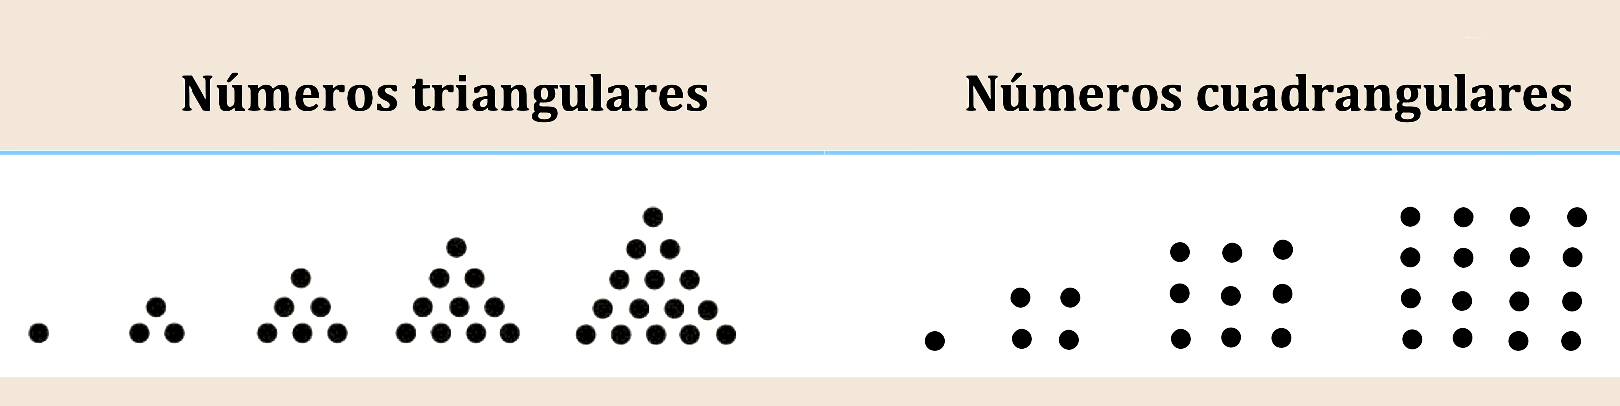
\includegraphics[width=0.75\textwidth]{img-suc/suc07.png}
\end{figure}


\end{mipropuesto}

\vspace{-8mm}
\begin{flushright}
\begin{footnotesize} \textcolor{gris}{\rotatebox{180}{ Nums. cuadrangulares: $\quad 1^2,\ 2^2,\ 3^2,\ 4^2,\ \cdots \ \to \ C_n=n^2$ }}	\end{footnotesize}
\end{flushright}
\vspace{-10mm}
\begin{flushright}
\begin{footnotesize} \textcolor{gris}{\rotatebox{180}{ Nums. triangulares. $\quad 1,\ 1+2,\ 1+2+3,\ 1+2+3+4,\ \cdots \ \to \ T_n=n(n+1)/2$ }}	\end{footnotesize}
\end{flushright}


%************
\begin{mipropuesto}

\begin{multicols}{2}

De la siguiente sucesión de cuadrados, calcula:

\vspace{3mm} a) Sucesión que define las áreas de cada cuadrado.	

b) Sucesión de las longitudes de sus lados.

c) Suma de las áreas de todos ellos.

\begin{figure}[H]
	\centering
	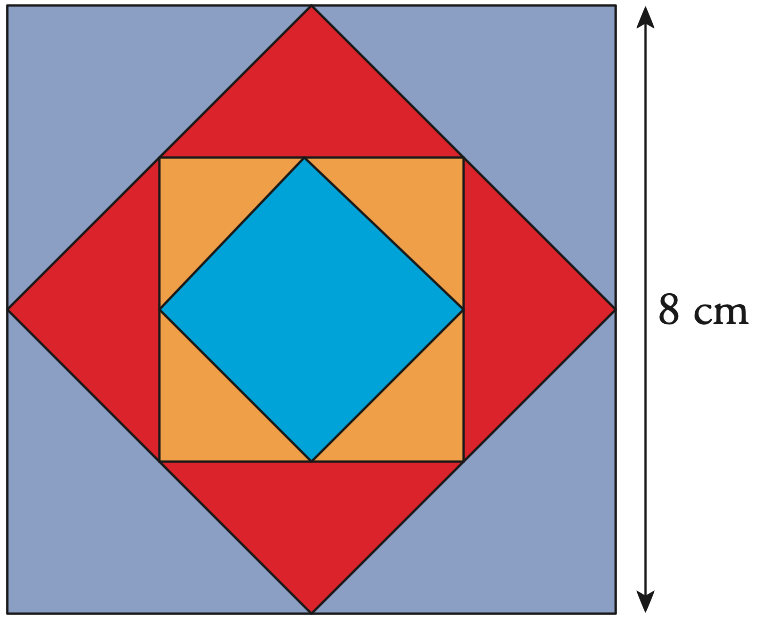
\includegraphics[width=0.35\textwidth]{img-suc/suc04.png}
\end{figure}


\end{multicols}

\end{mipropuesto}

\vspace{-8mm}
\begin{flushright}
\begin{footnotesize} \textcolor{gris}{\rotatebox{180}{ $a_n=2^{7-n};\qquad b_n=2^{\frac{7-n}{2}} \, \mathrm{cm} ;\qquad S_\infty=128 \, \mathrm{cm}^2$ }}	\end{footnotesize}
\end{flushright}



%**********
\begin{mipropuesto}

\begin{multicols}{2}

Considera un triángulo equilátero de 16 cm de lado. Se unen los puntos medios de sus lados para obtener 4 nuevos triángulo más pequeños. En estos triángulos se vuelven a unir los puntos medios, y así sucesivamente. Calcula:

a) Sucesión que define el área de los triángulos obtenidos.	

b) Sucesión de las longitudes de sus lados.

c) Sucesión de las áreas de todos ellos.

\begin{figure}[H]
	\centering
	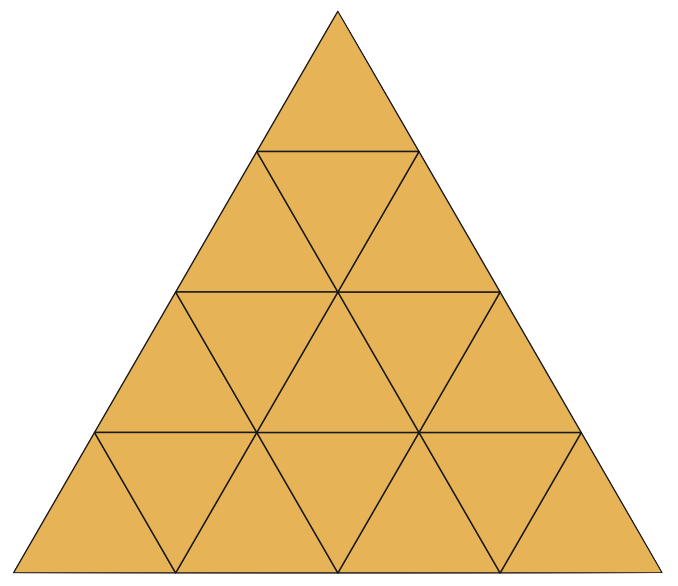
\includegraphics[width=0.4\textwidth]{img-suc/suc05.png}
\end{figure}


\end{multicols}

\end{mipropuesto}

\vspace{-8mm}
\begin{flushright}
\begin{footnotesize} \textcolor{gris}{\rotatebox{180}{ $a_n=4^{n-1};\qquad l_n=2^{5-n};\qquad a_n=2^{8-2n}\sqrt{3}$ }}	\end{footnotesize}
\end{flushright}

%********

\begin{mipropuesto}

Interpola 6 términos entre 1 y 10 que formen una PA.
\end{mipropuesto}

\vspace{-8mm}
\begin{flushright}
\begin{footnotesize} \textcolor{gris}{\rotatebox{180}{ $16/7,\ 25/7,\ 34/7,\ 43/7,\ 52/7,\ 61/7$ }}	\end{footnotesize}
\end{flushright}


%********

\begin{mipropuesto}

Interpola tres términos entre 1 y 16 para que formen una PG.
\end{mipropuesto}

\vspace{-8mm}
\begin{flushright}
\begin{footnotesize} \textcolor{gris}{\rotatebox{180}{ $r^4=16 \to |r|=2 \to r=\pm 2:\ \ \text{ Sol.: }\  \pm 2,\ 4,\ \pm 8$ }}	\end{footnotesize}
\end{flushright}



%********

\begin{mipropuesto}

En un examen la primera pregunta vale 2 puntos y cada una de las siguientes vale 3 puntos más que la anterior. Si en total hay 50 preguntas, ?`cuántos puntos vale el examen?
\end{mipropuesto}

\vspace{-8mm}
\begin{flushright}
\begin{footnotesize} \textcolor{gris}{\rotatebox{180}{ PA: 3775 }}	\end{footnotesize}
\end{flushright}



%********

\begin{mipropuesto}

Inicialmente hay 50 moscas en un laboratorio y, cada tres días, el número de moscas se duplica. ?`Cuántas moscas habrá al cabo de un mes?
\end{mipropuesto}

\vspace{-8mm}
\begin{flushright}
\begin{footnotesize} \textcolor{gris}{\rotatebox{180}{ PG (1mes=30 días). Habrá 16000 moscas. }}	\end{footnotesize}
\end{flushright}



%********

\begin{mipropuesto}

Los ángulos de un triángulo están en PA, si el ángulo intermedio vale $60^o$, ?`qué puedes afirmar de la distancia de la progresión?
\end{mipropuesto}

\vspace{-8mm}
\begin{flushright}
\begin{footnotesize} \textcolor{gris}{\rotatebox{180}{ (Dos ángulos han de sumar menos de $180^o$) $\quad$ $-60<d<60$ }}	\end{footnotesize}
\end{flushright}




%%%%%%%%%%%%%%%%%%%%%%%%%%%%.  problemas +.   %%%%%%%%%%%%%%%%%%%%
\newpage
\begin{adjustwidth}{50pt}{250pt}
\begin{cuadro-naranja}
\textbf{\huge{Problemas $\boldsymbol{+}$}}\normalsize{$\, $}
\end{cuadro-naranja}	
\end{adjustwidth}

\vspace{5mm}
\begin{enumerate}[\textbf{P$\boldsymbol +$} 1. ]

%
\item	Demostrar que las sucesivas medias de $n$ primeros términos de una progresión aritmética de distancia $d$ forman una progresión aritmética de distancia $d/2$.

\vspace{-6mm}
\begin{flushright}
\begin{footnotesize} \textcolor{gris}{\rotatebox{180}{ $x_n:\ PA[x_1,d/2]\, \  \text{ hay que demostrar que  } \ x_{n+1}-x_n=d/2$ }}

 \textcolor{gris}{\rotatebox{180}{ $a_n:\ PA[a_1,d]\qquad x_1=a_1,\ x_2=(a_1+a_2)/2,\ x_3=(a_1+a_2+a_3)/3,\ \cdots$ }}	\end{footnotesize}
\end{flushright}


%
\item	La suma de 18 números naturales consecutivos es un cuadrado perfecto, ?`cuál es el menor valor posible de la suma de ellos?

\vspace{-6mm}
\begin{flushright}
\begin{footnotesize} \textcolor{gris}{\rotatebox{180}{ $PA[a_1,\, d=1]\to \text{ cuadrado perfecto mínimo si  } a_1=4 \ \to \ S_{18}=15^2$ }}	\end{footnotesize}
\end{flushright}


%
\item	Si $a_n$ es PA y también PG y sabemos que $a_1=5$, ?`qué vale $a_5$? 

\vspace{-6mm}
\begin{flushright}
\begin{footnotesize} \textcolor{gris}{\rotatebox{180}{ $5$ en ambos casos. }}	\end{footnotesize}
\end{flushright}


%
\item	Fíjate en la siguiente figura, ?`puedes generalizar el resultado?

\begin{figure}[H]
	\centering
	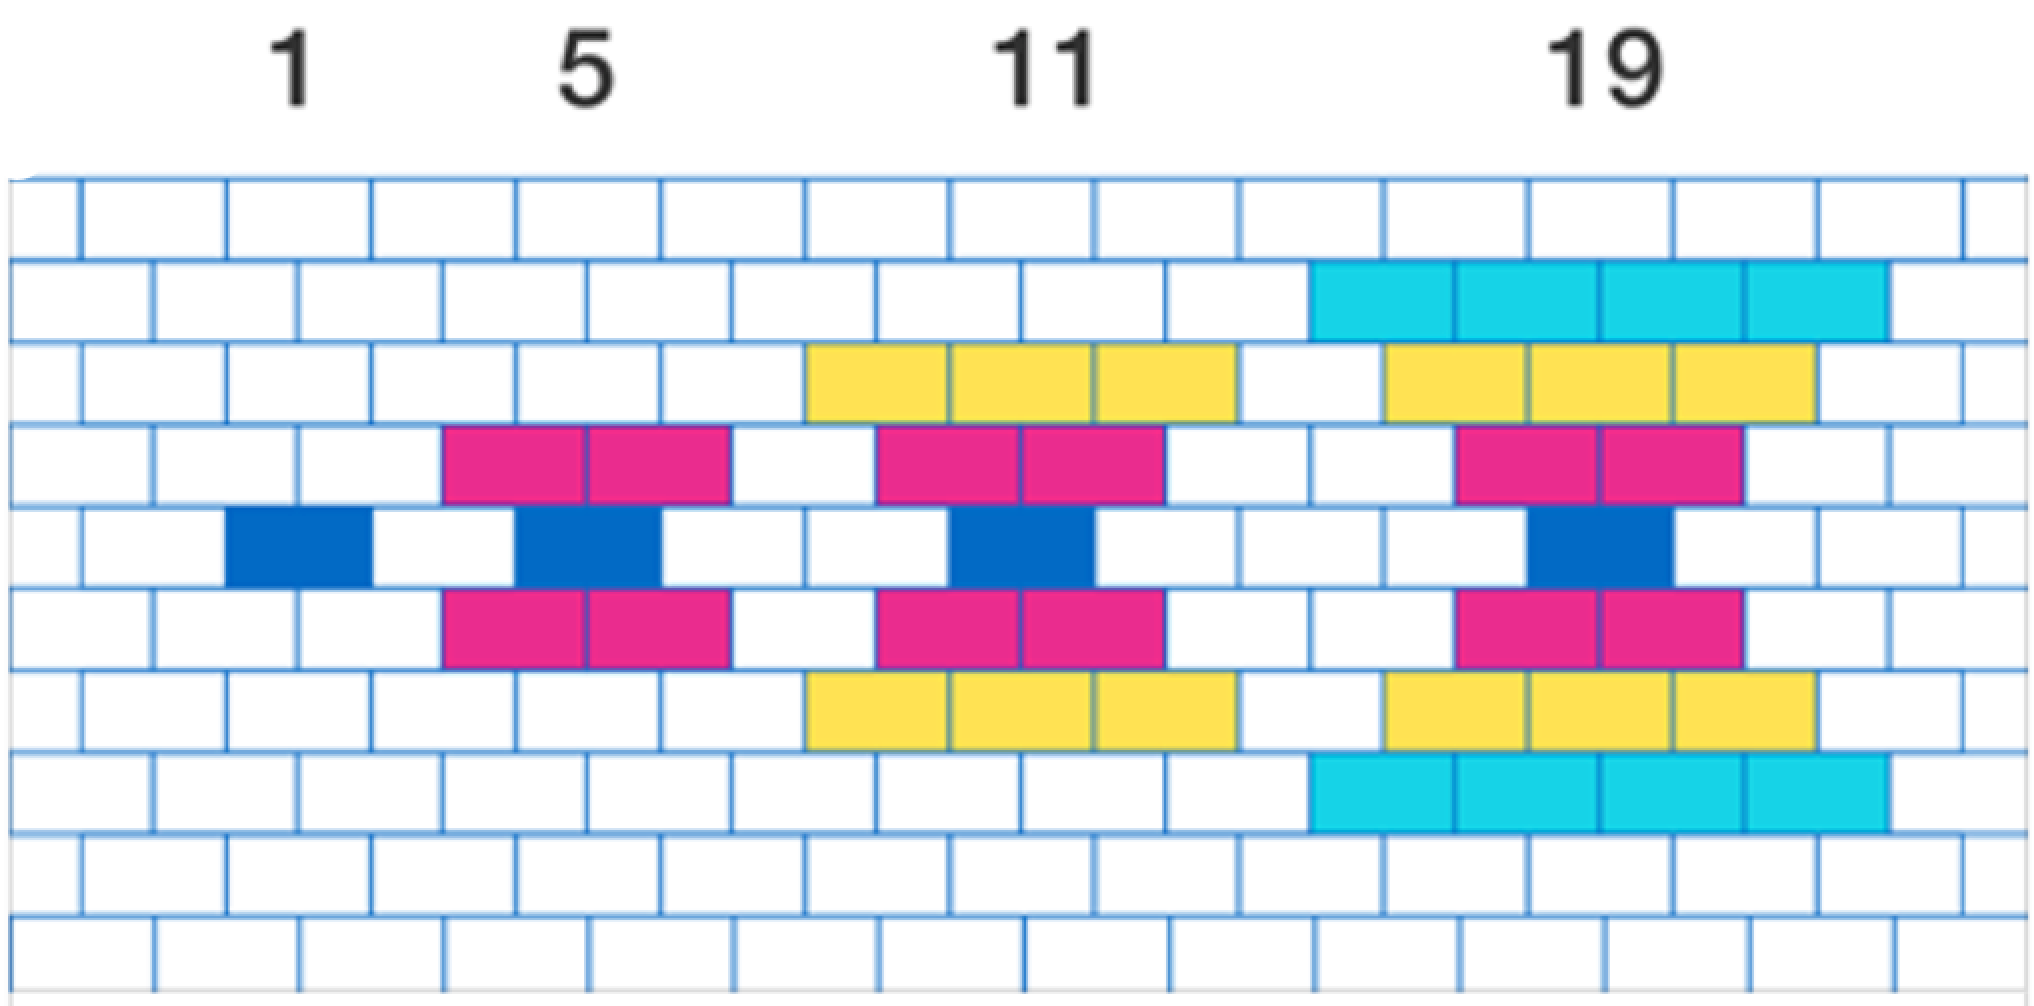
\includegraphics[width=0.5\textwidth]{img-suc/suc06.png}
\end{figure} 

\vspace{-10mm} %%%%%
\begin{flushright}
\begin{footnotesize} \textcolor{gris}{\rotatebox{180}{ Piensa en lo que ocurre a partir de la posición segunda.  $\quad a_1=1,\ \ a_n=n^2-n-1,\ \forall n\geq 2$}}	\end{footnotesize}
\end{flushright}


%
\item	Los primeros términos de una PG son: $ \ \sqrt{2}+1,\, 1,\ \sqrt{2}-1,\ \cdots $
La suma de \emph{todos} sus términos puede expresarse como $\ S_\infty=\dfrac{a+b\sqrt{c}}{d}.\ $ ?`Cuál es el valor mínimo de $a+b+c+d$? 

\vspace{-6mm}
\begin{flushright}
\begin{footnotesize} \textcolor{gris}{\rotatebox{180}{ $s_\infty=\frac{4+3\sqrt{2}}{2} \ \to \ a+b+c+d=11,\ $ valor mínimo pues expresión está simplificada al máximo. }}	\end{footnotesize}
\end{flushright}


%
\item	Si $f_n$ designa el término $n$-simo de la sucesión de Fibonacci \textcolor{gris}{$[ \ f_1=1,\ f_2=1,\ f_n=f_{n-1}+f_{n-2},\, \forall n>2 \ ]$} y conociendo que $f_{28}=317811$ y que $f_{24}=46368$, usando estos datos, determina el valor de $f_{26}$.

\vspace{-6mm}
\begin{flushright}
\begin{footnotesize} \textcolor{gris}{\rotatebox{180}{ Escribe $f_{26}$ en función de $f_{24}$ y $f_{28}$ usando la recurrencia de la sucesión. $\quad$ $f_{26}=121393$  }}	\end{footnotesize}
\end{flushright}


%
\item	En la sucesión $ \ a_1,a_2,a_3,\cdots \ $ se cumple que $a_1=a,\  a_3=b,\ a_{n+1}=a-n+a_{n+2}-1,\, \forall n\geq 2. \ $ Calcula la suma de los $2022$ primeros términos.

\vspace{-4mm}
\begin{flushright}
\begin{footnotesize} \textcolor{gris}{\rotatebox{180}{y, a partir de ahí, la sucesión se repite. Como $2022=337\times 6 \to S_{2020}=337\times 6$ }}	\end{footnotesize}

\begin{footnotesize} \textcolor{gris}{\rotatebox{180}{ Busca los primeros términos de la sucesión hasta que caigas en la cuenta de que $a_1+\cdots +a_6=6$  }}	\end{footnotesize}
\end{flushright}

%
\item	Dados los tres primeros términos de una PG: $\ \sqrt{7},\ \sqrt[3]{7},\ \sqrt[6]{7}\, , \ $ ?`cuál es el siguiente término de la progresión?

\vspace{-6mm}
\begin{flushright}
\begin{footnotesize} \textcolor{gris}{\rotatebox{180}{ 1 }}	\end{footnotesize}
\end{flushright}

%
\item	Los números $\ \log(a^3b^7),\ \log(a^5b^{12}),\ \log(a^8b^{15})\ $ son los tres primeros términos de una PA en la que $\ \log(b^n)\ $ es el duodécimo termino. ?`Qué vale $n$?

\vspace{-6mm}
\begin{flushright}
\begin{footnotesize} \textcolor{gris}{\rotatebox{180}{ 112 }}	\end{footnotesize}
\end{flushright}

%
\item	En una PA de 9 términos el quinto es 4. ?`Cuánto suman los 9 términos?

\vspace{-6mm}
\begin{flushright}
\begin{footnotesize} \textcolor{gris}{\rotatebox{180}{ Equidistancia, $a_5$ es el término central. $\quad$ sol: $\ 36$ }}	\end{footnotesize}
\end{flushright}


\end{enumerate}



%%%%%%%%%%%%%%%%%%%%%%%%%%%%%%%%%%%%
\newpage
\section{Resumen del tema}
\begin{tikzpicture}
	\fill [left color=red!50, right color=teal!50] (0,0) rectangle (3.5,.1);
	\fill [left color=teal!50, right color=blue!50] (3.5,0) rectangle (7.5,.1);
	\end{tikzpicture}
\vspace{1cm}

\begin{myblock}{Resumen: \emph{``Sucesiones''}}

\vspace{2mm}\textbf{Progresión aritmética}: cada término se obtiene del anterior al sumar una cantidad constante llamada distancia.

$$\boxed{ \ \boldsymbol{a_n\ = \ a_1\, + \, (n-1)\, d}  \ } 
\qquad \qquad
 \boxed{\ \boldsymbol{ S_n\ = \ \dfrac{a_1+a_n}{2}\ n } \ }$$
 
\vspace{5mm} \textbf{Progresión geométrica}: cada término se obtiene del anterior al multiplicar una cantidad constante llamada razón.

$$\boxed{\ \boldsymbol{ a_n\ = \ a_1\, r^{n-1} } \ }
\qquad \qquad	
\boxed{\ \boldsymbol{ S_n\ = \ \dfrac{a_n\, r - a_1}{r-1} } \ }$$

$$\boxed{\ \boldsymbol{ S_\infty \ = \ \dfrac{a_1}{1-r}  } \ } \ \ \leftrightarrow \ \ |r|<1
\qquad \qquad	
\boxed{\ \boldsymbol{ P_n\ = \ \sqrt{(a_1\, a_n)^n} } \ }$$

\vspace{5mm} \textbf{Interpolar} $m$ medios (aritméticos o geométricos) entre dos números dados $a$ y $b$ es encontrar $m$ números $a_1,a_2,\cdots , a_m$ de modo que la sucesión $a,a_1,a_2,\cdots , a_m,b$ formen una progresión (aritmética o geométrica).

\vspace{5mm}$\triangleright \quad   \{a_n\} \ $ es una sucesión \textbf{monótona creciente } si $\ a_{n+1}>a_n\, , \ \ \forall n\in \mathbb N$


\vspace{2mm}$\triangleright \quad \{a_n\} \ $ es una sucesión \textbf{monótona decreciente } si $\ a_{n+1}<a_n\, , \ \ \forall n\in \mathbb N$

\vspace{5mm}$\triangleright \quad \{a_n\} \ $ es una sucesión\textbf{ acotada } si $\ \exists K \in \mathbb R \, / \,  |a_n|\leq K , \ \ \forall n\in \mathbb N$

\vspace{5mm}$\triangleright \quad \{a_n\} \ $ es una sucesión\textbf{ convergente  } si $\ \exists \ \underset{n\to \infty}{\mathrm{lim}}\, a_n$

\vspace{2mm}

\end{myblock}

















\begin{comment}


%%%%%%%%%%%%%%% EJER PPTO
Un atleta quiera preparar una carrera y entrenará, de forma constante, el número de metros que corre cada día. Cada día correrá una cantidad de metros constante más que el día anterior.

Empieza a correr el lunes 280 m y quiere llegar a correr el domingo 1km. ?`Cuánto debe correr cada día.
%%%%%%%%%%%%%%%%%%%%%




%%%%%%%%%%%%%%%%%%%%%%%%%%%%%%%%%%%. SECCIONES
\chapter{texto}
\begin{tikzpicture}
	\fill [left color=red!50, right color=teal!50] (0,0) rectangle (6.5,.2);
	\fill [left color=teal!50, right color=blue!50] (6.5,0) rectangle (11.5,.2);
	\end{tikzpicture}

\vspace{1cm}
\section{texto}
\begin{tikzpicture}
	\fill [left color=red!50, right color=teal!50] (0,0) rectangle (3.5,.1);
	\fill [left color=teal!50, right color=blue!50] (3.5,0) rectangle (7.5,.1);
	\end{tikzpicture}
\vspace{0.5cm}

\subsection{texto}
\begin{tikzpicture}
	\fill [left color=red!50, right color=teal!50] (0,0) rectangle (3.5,.01);
	\fill [left color=teal!50, right color=blue!50] (3.5,0) rectangle (7.5,.01);
	\end{tikzpicture}
\vspace{0.5cm}


%%%%%%%%%%%%%%%%%%%%%%%%%%%%%%%%%%%. \begin{ ------>. 
detsacado;  cuadro-naranja;  cuadro-gris;  miejercicio (solución extensa);  mipropuesto (solución corta y fuera del cuadro)

%%%%%%%%%%%%%%%%%%%%%%%%%%%%%%%%%%%. CURIOSIDAD
\vspace{1cm}
\color{ForestGreen!80}
\rule{250pt}{0.2pt}
Texto
\vspace{-8mm}
\begin{flushright}
\rule{250pt}{0.2pt}		
\end{flushright}	
\color{black}




IMAGENES%******************************
\begin{figure}[H]
	\centering
	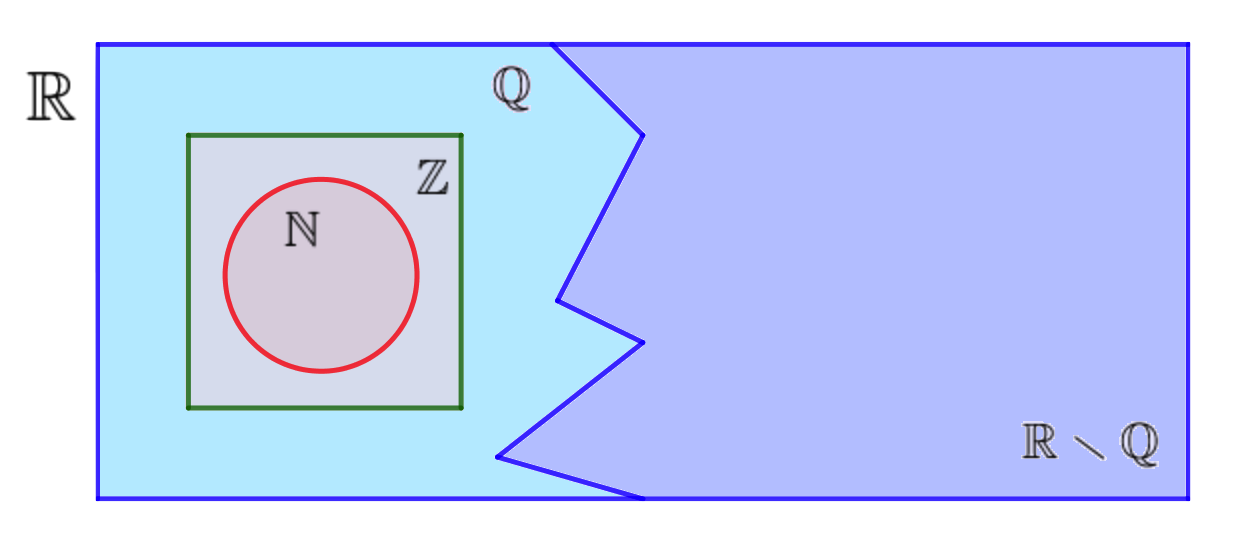
\includegraphics[width=0.75\textwidth]{img-reales/reales18.png}
	\end{figure}
\end{comment} %
\chapter{Polinomios y fracciones algebraicas}
\begin{tikzpicture}
	\fill [left color=red!50, right color=teal!50] (0,0) rectangle (6.5,.2);
	\fill [left color=teal!50, right color=blue!50] (6.5,0) rectangle (11.5,.2);
	\end{tikzpicture}
	
	
\vspace{15mm}


\begin{adjustwidth}{40pt}{40pt}
\begin{cuadro-gris}

	\begin{multicols}{2}
	$\triangleright \quad$ Polinomios. Operaciones.
	
	$\triangleright \quad$ Regla de Ruffini y teorema del resto.
	
	$\triangleright \quad$ Factorización de polinomios.
	
	$\triangleright \quad$ Fracciones algebráicas.
	\end{multicols}
	
\end{cuadro-gris}
\end{adjustwidth}


\vspace{1cm}

\begin{myexampleblock}{Aritmética vs Álgebra}
\vspace{2mm} \textbf{Aritmética}: realmente es algo que se utiliza a diario sin darse cuenta, incluye todo lo relacionado a números. La palabra aritmética desciende de un término griego (aritmo) el cual significa número. Es una rama básica de las matemáticas y con ésta se trabaja tradicionalmente con las 4 operaciones básicas que solemos utilizar: resta, suma, división y multiplicación. También existe una aritmética avanzada o superior, conocida como \emph{teoría de números}.


\vspace{2mm} \textbf{Álgebra}: también es una rama perteneciente a las matemáticas; la palabra  derivad de un término árabe (al-Jabr), fueron quienes más contribuyeron a la formación de esta rama; al-Jabr realmente era un término médico que significaba algo así como poner en orden las piezas rotas; los árabes inventaron el álgebra con el fin de poder razonar con lógica, donde lo importante era el razonamiento y no los valores, debido a esto tenía letras y no números, puesto que lo que buscaban era poder razonar sin importar las cifras. Dentro de las matemáticas podemos poner al álgebra como en un segundo nivel seguido de la aritmética. Lo que la diferencia principalmente de la aritmética es que no trabaja solo con números, sino que mezcla estos con otros valores que son desconocidos (incógnitas o variables).

\vspace{2mm} \textcolor{gris}{Fuente: https://educar.doncomos.com/saber-diferenciar-algebra-aritmetica}	

\end{myexampleblock}


\begin{figure}[H]
	\centering
	
\includegraphics[width=0.5\textwidth]{img-pol/pol02.png}
\end{figure}



\vspace{1cm}
\section{Polinomios}
\begin{tikzpicture}
	\fill [left color=red!50, right color=teal!50] (0,0) rectangle (3.5,.1);
	\fill [left color=teal!50, right color=blue!50] (3.5,0) rectangle (7.5,.1);
	\end{tikzpicture}
\vspace{0.5cm}


Un \textbf{monomio} es una expresión algebraica formada por un número (\emph{coeficiente}) y una o varias letras (variables) elevadas a exponentes naturales (\emph{parte literal}).

Se llama \text{grado del monomio} al exponente de la parte literal (si es de una sola variable) o la suma de los exponentes (si el monomio es de varias variables).

Dos momonios son \emph{semejantes} si tienen la misma parte literal.

\vspace{5mm}
\begin{definition}[ Polinomio]

Un \textbf{polinomio} de una variable es una expresión del tipo:

$$\boldsymbol{ p(x)\ = \ a_0x^n+a_1x^{n-1}+\cdots +a_{n-2}x^2+a_{n-1}x+a_0 }$$	

$a_i: \ i=0,1,2,\cdots n \ $ son los coeficientes.

\end{definition}

\vspace{3mm}
\begin{definition}

\vspace{2mm}\textbf{Grado de un polinomio} es el exponente de la máxima potencia de la variable (el mayor grado de los monomios que forman el polinomio).
Cada uno de los monomios que forman el polinomio recibe el nombre de \textbf{término}. Los polinomios de dos términos se llaman \emph{binomios}, los de tres \emph{trinomios}.
\end{definition}


\vspace{3mm}
\begin{definition}[ Valor numérico de un polinomio]

\textbf{Valor numérico} del polinomio $\ p(x) \ $ en $\ x=a\in \mathbb R\ $ es el número que resulta al sustituir en el polinomio $x$ por $a$, es decir, calcular $\ p(a)$.	
\end{definition}

\vspace{5mm}

\begin{miejemplo}

El grado de $\ -3x^4\ $ es $\ 4$, el de $\ 23x^3y^2z \ $ es $\ 6=3+2+1$.

\vspace{2mm} Si $p(x)=x^4+7x+1 \ \to \ $ el valor numérico en $x=-2$ es $\ p(-2)=(-2)^4+7\, (-2)+1=3$. El grado de $p(x)$ es $4$.
\end{miejemplo}

\vspace{1cm}
\section{Operaciones con polinomios}
\begin{tikzpicture}
	\fill [left color=red!50, right color=teal!50] (0,0) rectangle (3.5,.1);
	\fill [left color=teal!50, right color=blue!50] (3.5,0) rectangle (7.5,.1);
	\end{tikzpicture}

\vspace{0.5cm}


\begin{figure}[H]
	\centering
	\includegraphics[width=0.5\textwidth]{img-pol/pol03.png}
\end{figure}



\vspace{0.75cm}

\subsection{Suma y producto de polinomios}
\begin{tikzpicture}
	\fill [left color=red!50, right color=teal!50] (0,0) rectangle (3.5,.01);
	\fill [left color=teal!50, right color=blue!50] (3.5,0) rectangle (7.5,.01);
	\end{tikzpicture}
\vspace{0.5cm}

$\triangleright \qquad 3(3x^3-4x+1)-2(4x^2-5x)=9x^3-12x+3-8x^2+10x=9x^3-8x^2-2x+3$

$\triangleright \qquad (2x^2+1)\cdot (3x^3-2x+5)=6x^4-4x^3+10x^2+3x^2-2x+5=6x^4-4x^3+13x^2-2x+5$

\begin{itemize}
\item El producto de un número $k$ por un polinomio $p(x)$ es el polinomio $k\, p(x)$ en que todos los coeficientes de $p(x)$ se han multiplicado por $k$.
\item La suma de polinomios verifica las propiedades \emph{conmutativa} \textcolor{gris}{$[ \ p(x)+q(x)=q(x)+p(x) \ ]$} y \emph{asociativa} \textcolor{gris}{$[ \ p(x)+(q(x)+r(x))=(p(x)+q(x))+r(x) \ ]$}. El neutro para la suma es el polinomio nulo, $0$. El \emph{opuesto} a un polinomio $p(x)$ es el polinomio $-p(x)$, en que todos los coeficientes han cambiado de signo, de ese modo, $p(x)-q(x)=p(x)+(-q(x))$.
\item El producto de polinomios verifica las propiedades \emph{conmutativa} \textcolor{gris}{$[ \ p(x)\cdot q(x)=q(x) \cdot p(x) \ ]$} y \emph{asociativa} \textcolor{gris}{$[ \ p(x)\,(q(x)\, r(x))=(p(x)\ q(x))\, r(x) \ ]$}. El neutro para el producto es el polinomio unidad, $1$. El producto de polinomios no tiene \emph{inverso}.
\item Se cumple la propiedad \emph{distribituva} del producto respecto de la suma: $\ p(x)\, (q(x)+r(x))=p(x)\, q(x)+p(x)\, r(x)$. Esta  propiedad, leída de derecha a izquierda, es la que permite sacar \emph{factor común}.
\end{itemize}



\subsection{Productos notables}
\begin{tikzpicture}
	\fill [left color=red!50, right color=teal!50] (0,0) rectangle (3.5,.01);
	\fill [left color=teal!50, right color=blue!50] (3.5,0) rectangle (7.5,.01);
	\end{tikzpicture}
\vspace{0.5cm}

Son casos particulares del binomio de Newton que, por la frecuencia con que aparecen, vale la pena recordar.

$$ \boldsymbol{ \boxed{ \ \subrayado{ \ (a\pm b)^2 \ = \ a^2 \pm 2ab+b^2  \ } \ } \ ;\qquad \qquad \boxed{ \ \subrayado{ \ (a+b) \, (a-b) \ = \ a^2-b^2} \ } \ } $$

\color{gris}

$$(a\pm b)^3 \ = \ a^3\pm 3a^2b\pm 3ab^2+b^3\, ; \qquad \qquad a^3\pm b^3 \ = \  (a\pm b)\, (a^2\mp ab+b^3)$$

$$(a+b+c)^2 \ = \ a^2+b^2+c^2 \, + \, 2ab \, + \, 2ac \, + \, 2bc$$

\color{black}

\begin{figure}[H]
	\centering
	
\includegraphics[width=0.35\textwidth]{img-pol/pol04.png}
\end{figure}

\subsection{División de polinomios}
\begin{tikzpicture}
	\fill [left color=red!50, right color=teal!50] (0,0) rectangle (3.5,.01);
	\fill [left color=teal!50, right color=blue!50] (3.5,0) rectangle (7.5,.01);
	\end{tikzpicture}
\vspace{0.5cm}



% Please add the following required packages to your document preamble:
% \usepackage{multirow}
\begin{table}[H]
\centering
\begin{tabular}{llllll}
\multicolumn{1}{l|}{$D(x)$} & $\ d(x)\ $ & $\qquad$ & \multirow{2}{*}{$D(x)=d(x)\, c(x)+r(x)$} & $\qquad$ & \multirow{2}{*}{$\dfrac{D(x)}{d(x)}=c(x)+\dfrac{r(x)}{d(x)}$} \\ \cline{2-2}
$r(x)$ & $\ c(x)\ $ &  &  &  & 
\end{tabular}
\end{table}

\begin{itemize}
\item Para efectuar la división, grado $D(x) \geq $ grado $d(x)$	
\item Si $r(x)=0 \ \to \ $ la división es exacta.
\item La división acaba al obtener grado $r(x) \leq $ grado $d(x)$
\end{itemize}

\vspace{5mm}
Recordemos como efectuamos la división entre números.

\underline{División numérica}:
\begin{table}[H]
\centering
\small
\begin{tabular}{llrrrrl}
\textcolor{gris}{$183\, :\, 27 \to \textcolor{red}{6}\cdots $} &  & 1 & 8 & 3 & \multicolumn{1}{r|}{4} & $\quad 27$ \\ \cline{7-7} 
\textcolor{gris}{$6\cdot 27$} & \scriptsize{\textcolor{gris}{$\overrightarrow{\text{su opuesto}} \qquad$}} & \textcolor{gris}{-1} & \textcolor{gris}{6} & \textcolor{gris}{2} &  & $\quad \textcolor{red}{6}\, \textcolor{blue}{7}$ \\ \cline{3-5}
\textcolor{gris}{$214\, : \, 27 \to \textcolor{blue}{7}\cdots$} &  &  & 2 & 1 & 4 &  \\
\textcolor{gris}{$7\cdot 27$} & \scriptsize{\textcolor{gris}{$\overrightarrow{\text{su opuesto}} \qquad$}} &  & \textcolor{gris}{-1} & \textcolor{gris}{8} & \textcolor{gris}{9} &  \\ \cline{5-6}
 &  &  &  & 2 & 5 & 
\end{tabular}
\end{table}

Del mismo modo, para dividir polinomios el procedimiento es:

\underline{División de polinomios}:
\begin{table}[H]
\centering
\begin{tabular}{llrrrrrll}
\textcolor{gris}{$6x^2\ :\ 2x^2= \textcolor{red}{3x^2}$} &  & $6x^4$ & $+5x^3$ & $+x^2$ & $+3x$ & $-2$ & \multicolumn{1}{l|}{$\quad$} & $2x^2-x+3$ \\ \cline{9-9} 
\textcolor{gris}{$3x^2\, (2x^2-x+3)$} & \scriptsize{\textcolor{gris}{$\overrightarrow{\text{su opuesto}} \qquad$}} & $-6x^4$ & $+3x^3$ & $-9x^2$ &  &  &  & $\textcolor{red}{3x^2}\, + \, \textcolor{blue}{4x}\, -\, \textcolor{DarkGreen}{2}$ \\ \cline{3-5}
\textcolor{gris}{$8x^3\ : \ 2x^2=\textcolor{blue}{4x}$} &  &  & $8x^3$ & $-8x^2$ & $+3x$ & $-2$ &  &  \\
\textcolor{gris}{$4x\, (2x^2-x+3)$} & \scriptsize{\textcolor{gris}{$\overrightarrow{\text{su opuesto}}$}} &  & $-8x^3$ & $+4x^2$ & $-12x$ &  &  &  \\ \cline{4-6}
\textcolor{gris}{$-4x^2 \  : \ 2x^2=\textcolor{DarkGreen}{-2}$} &  &  &  & $-4x^2$ & $-9x$ & $-2$ &  &  \\
\textcolor{gris}{$-2\, (2x^2-x+3)$} & \scriptsize{\textcolor{gris}{$\overrightarrow{\text{su opuesto}}$}} &  &  & $4x^2$ & $-2x$ & $+6$ &  &  \\ \cline{5-7}
 &  &  &  &  & $-11x$ & $+4$ &  & 
\end{tabular}
\end{table}

\vspace{5mm}

%%%%%
\begin{miejercicio}

Calcula: $\quad (2x+1)(3x-2)(5x-1)$

\vspace{-2mm}
\rule{250pt}{0.1pt}	

$(2x+1)(3x-2)(5x-1)=((2x+1)(3x-2))\, (5x-1)= (6x-4x^2+3-2x)(5x-1)=(-4x^2+4x+3)(5x-1)=-20x^3+20x^2+15x+4x^2-4x-3=-20x^3+24x^2+11x-3$
\end{miejercicio}

%%%%% 
\vspace{5mm}
\begin{miejercicio}

Extrae factor común: $\quad 28x^5-12x^4+16x^3$

\vspace{-2mm}
\rule{250pt}{0.1pt}	

$28x^5-12x^4+16x^3=4x^3\, (7x^2-3x+4)$
\end{miejercicio}

%%%%%
\vspace{5mm}
\begin{miejercicio}

Calcula: $\quad a)\ \left( \dfrac{2x}{3}-\dfrac{3}{2} \right)^2 ; \qquad b)\ (3x+4)(3x-4)\, ; \qquad c)\ (-3x-2)(-3x+2)$

\vspace{-2mm}


\rule{250pt}{0.1pt}	

\vspace{2mm} $\triangleright \quad  a)\ \left( \dfrac{2x}{3}-\dfrac{3}{2} \right)^2 =\left( \dfrac{3x}{2} \right)^2 - 2 \, \dfrac{3x}{2} \, \dfrac{2}{3} + \left( \dfrac{2}{3} \right)^2=\dfrac{4x^2}{9}-2x+\dfrac{9}{4} $


\vspace{2mm} $\triangleright \quad b)\ (3x+4)(3x-4) = (3x)^2-4^2=9x^2-16$


\vspace{2mm} $\triangleright \quad c)\ (-3x-2)(-3x+2)=-(3x+2)(3x-2)=-(9x^2-4)=4-9x^2 $
\end{miejercicio}

%%%%%
\vspace{5mm}
\begin{miejercicio}

Calcula: $\quad (3x^3-2x^2+5)\, : \, (2x^2-x+1) \quad$  Comprueba el resultado.

\vspace{-2mm}
\rule{250pt}{0.1pt}	

\begin{table}[H]
\centering
\begin{tabular}{rrrrll}
$3x^3$ & $-2x^2$ &  & $+5$ & \multicolumn{1}{l|}{$\quad$} & $2x^2-x+1$ \\ \cline{6-6} \\
$-3x^3$ & $+\dfrac 3 2 x^2$ & $-\dfrac 3 2 x$ &  &  & $\dfrac 3 2 x -\dfrac 1 4$ \\  \\ \cline{1-3} \\ 
 & $-\dfrac 1 2 x^2$ & $-\dfrac 3 2 x$ & $+5$ &  &  \\
 & $\dfrac 1 2 x^2$ & $-\dfrac 1 4 x$ & $+\dfrac 1 4 $ &  &  \\ \\ \cline{2-4} \\
 &  & $-\dfrac 7 4 x$ & $+\dfrac{21}{4}$ &  & 
\end{tabular}
\end{table}


Prueba de la división: $\quad (2x^2-x+1)\left( \dfrac 3 2 x-\dfrac 1 4 \right) \, + \, \left( -\dfrac 7 4 x + \dfrac{21}4 \right)=$

$=\left( 3x^3-\dfrac 1 2 x^2 -\dfrac 3 2 x^2 +\dfrac 1 4 x + \dfrac 3 2 x-\dfrac 1 4 \right) \, + \, \left( -\dfrac 7 x x + \dfrac{21}4 \right)=$

$=\left( 3x^3-2x^2+\dfrac 7 4 x -\dfrac 1 4 \right) \, + \, \left( -\dfrac 7 x x + \dfrac{21}4 \right) \ = \ 3x^3-2x^2+5$ \textcolor{gris}{\QED}

\vspace{5mm} $ \dfrac{(3x^3-2x^2+5)}{(2x^2-x+1) } \ = \ \left( \dfrac 3 2 x -\dfrac 1 4  \right) \, (2x^2-x+1) \ + \ \left( -\dfrac 7 4 x +\dfrac {21}4 \right)$

\end{miejercicio}

%%%%%
\begin{miejercicio}

Encuentra dos polinomios tales que al dividirlos el cociente sea $p(x)=x^2-x-3$ y el resto $q(x)=-3x^2-1$.

\vspace{-2mm}
\rule{250pt}{0.1pt}	

Sean $A(x)$ y $B(x)$ los polinomios buscados, por la prueba de la división, $A(x)=B(x)\, p(x) \, + \, q(x)$

\vspace{2mm} La respuesta es infinita, para cualquier $B(x)$ que nos inventemos, obtenemos el $A(x)$ correspondiente. Como pasa con los números \textcolor{gris}{$\quad  \dfrac 3 2 ; \, \dfrac {4}{3}; \,  \dfrac{-8}{-7} ; \, \cdots $ todos tienen el mismo cociente $1$ y el mismo resto $1$, $D=d(1)+(1) \ \forall d \, \exists D$}.

\vspace{2mm} Eso sí, al ser el resto un polinomio de orden 2, el divisor ha de ser un polinomio de tercer grado o superior.

\vspace{2mm} Aplicando la prueba de la división, $A=B\, p+q$ obtenemos, para cada $B$ el $A$ correspondiente.

\vspace{2mm} Por ejemplo, para $B=x^3-2$, se obtiene $A(x)=(x^3-2)(x^2-x-3)+(-3x^2-1)=x^5-x^4-3x^3-5x^2+2x+5$
\end{miejercicio}




\section{Regla de Ruffini. Teorema del resto}
\begin{tikzpicture}
	\fill [left color=red!50, right color=teal!50] (0,0) rectangle (3.5,.1);
	\fill [left color=teal!50, right color=blue!50] (3.5,0) rectangle (7.5,.1);
	\end{tikzpicture}
\vspace{0.5cm}

El método de Ruffini es un algoritmo muy útil en las divisiones de polinomios en que el denominador sea un polinomio del tipo $\boldsymbol{x-a}$

\vspace{5mm}
\begin{multicols}{2}
\begin{table}[H]
\centering
\begin{tabular}{rrrrr}
$2x^3$ & \textcolor{DarkGreen}{$-3x^2$} & $-5x$ & \multicolumn{1}{r|}{$+7$} & \textcolor{Brown}{$ x-2 \quad $} \\ \cline{5-5} 
$-2x^3$ & \textcolor{DarkGreen}{$+4x^2$} &  &  & \textcolor{red}{$2x^2+x-3$} \\ \cline{1-2}
 & $x^2$ & \textcolor{DarkGreen}{$-5x$} & $+7$ &  \\
 & $-x^2$ & \textcolor{DarkGreen}{$+2x$} &  &  \\ \cline{2-3}
 &  & $-3x$ & \textcolor{DarkGreen}{$+7$} &  \\
 &  & $3x$ & \textcolor{DarkGreen}{$-6$} &  \\ \cline{3-4}
 &  &  & \textcolor{NavyBlue}{$1$} & 
\end{tabular}
\end{table}
\begin{center}\textbf{\underline{Regla de Ruffini}}: \end{center}
	
\begin{table}[H]
\centering
\begin{tabular}{rrrrr}
 & \textcolor{gris}{$2x^3$} & \textcolor{gris}{$-3x^2$} & \textcolor{gris}{$-5x$} & \textcolor{gris}{$+7$} \\
\multicolumn{1}{r|}{\textcolor{gris}{$x-\boxed{2}$}} & 2 & \textcolor{DarkGreen}{-3} & \textcolor{DarkGreen}{-5} & \textcolor{DarkGreen}{7} \\
\multicolumn{1}{r|}{\textcolor{Brown}{2}} &  & \textcolor{DarkGreen}{4} & \textcolor{DarkGreen}{2} & \textcolor{DarkGreen}{-6} \\ \hline
\multicolumn{1}{r|}{} & \textcolor{red}{2} & \textcolor{red}{1} & \multicolumn{1}{r|}{\textcolor{red}{-3}} & \textcolor{NavyBlue}{1} \\ \cline{5-5} 
 & \textcolor{gris}{$2x^2$} & \textcolor{gris}{$+x$} & \textcolor{gris}{$-3$} & 
\end{tabular}
\end{table}
\end{multicols}

Se escriben los coeficientes del polinomio dividendo completo y ordenado, \textbf{si falta algún término hay que poner un cero}. Se hace la cruz típica del método de Ruffini y se coloca el $a$ del polinomio divisor $x-2$ a la izquierda de la cruz, en este caso \textcolor{Brown}{2}.

Bajamos el primer coeficiente del polinomio dividendo, \textcolor{red}{$2$} y multiplicamos por \textcolor{Brown}{2}, el resultado, 	\textcolor{DarkGreen}{4} se coloca debajo del segundo coeficiente del dividendo y se suma, -3+\textcolor{DarkGreen}{4}=\textcolor{Red}{1}. Se procede del mismo moda hasta acabar.

Como el divisor es de primer grado, el cociente será un de grado menos que el dividendo, sus coeficientes aparecen en la última fila en rojo. El resto de la división será un polinomio de orden cero, un número; aparece en azul.

\begin{table}[H]
\centering
\begin{tabular}{llccccl}
 &  &  & $\boxed{2\times 2=\textcolor{red}{4}}$ & $\boxed{1\times 2=\textcolor{red}{2}}$ & $\boxed{-3\times 2=\textcolor{red}{-6}}$ & \multicolumn{1}{c}{} \\ \\
 & \multicolumn{1}{l|}{} & $\quad 2$ & -3 & -5 & 7 &  \\
$a$  del divisor $x-a$ & \multicolumn{1}{l|}{$\quad 2$} & $\quad \downarrow$ & \textcolor{red}{4} & \textcolor{red}{2} & \textcolor{red}{-6} &  \\ \cline{2-6}
coeficientes del cociente & \multicolumn{1}{l|}{} & $\quad 2$ & \textcolor{blue}{1} & \multicolumn{1}{c|}{\textcolor{blue}{-3}} & \textcolor{blue}{1} & Resto \\ \cline{6-6} \\
 &  &  & $\boxed{-3+4=\textcolor{blue}{1}}$ & $\boxed{-5+2=\textcolor{blue}{-3}}$ & $\boxed{7-6=\textcolor{blue}{1}}$ & \multicolumn{1}{c}{}
\end{tabular}
\end{table}


\vspace{5mm}
\begin{miejemplo}

Divide: $\quad (3x^4-30x^2-7x+2) 	\,  :\, (x+3) $

\begin{table}[H]
\centering
\begin{tabular}{rrrrrr}
 & \textcolor{gris}{$3x^4$} &  & \textcolor{gris}{$-30x^2$} & \textcolor{gris}{$-7x$} & \textcolor{gris}{$+2$} \\
\multicolumn{1}{r|}{\textcolor{gris}{$x-\boxed{-3}$}} & 3 & \textbf{0} & -30 & -7 & 2 \\
\multicolumn{1}{r|}{-3} &  & -9 & 27 & 9 & -6 \\ \hline
\multicolumn{1}{r|}{} & 3 & -9 & -3 & \multicolumn{1}{r|}{2} & -4 \\ \cline{6-6} 
 & \textcolor{gris}{$3x^3$} & \textcolor{gris}{$-9x^2$} & \textcolor{gris}{$-3x$} & \textcolor{gris}{$+2$} & 
\end{tabular}
\end{table}
Cociente: $\ 3x^3-9x^2-3x+2\, ; \ $ resto: $\ -4$ 

\vspace{2mm} Nótese el \emph{cero} que hemos colocado como coeficiente de $x^3$ en la fila de Ruffini.
\end{miejemplo}

\vspace{5mm}

\begin{miejercicio}

Realiza las divisiones siguientes:
\hspace{1.1cm} $a)\ \ (3x^4-5x^3-8x^2-5) \, : \, (x-3)\, ;$

\vspace{2mm}$b) \ \ (4x^3-2x+3)\, : \, (x+1)	\, ;\quad  \qquad \qquad c)\ \ (5x^3+7x^2+3x-5)\, : \, (2x+1)$

\rule{250pt}{0.1pt}

\begin{multicols}{2}
a)
\begin{table}[H]
\centering
\begin{tabular}{r|rrrrr}
 & 3 & 5 & -8 & 0 & 5 \\
3 &  & 9 & 12 & 12 & 36 \\ \hline
 & 3 & 4 & 4 & \multicolumn{1}{r|}{12} & 31 \\ \cline{6-6} 
\end{tabular}
\end{table}
Cociente: $\ 3x^3+4x^4+4x+12\, ; \ $ 

Resto: $\ 31$

b)
\begin{table}[H]
\centering
\begin{tabular}{r|rrrr}
 & 4 & 0 & -2 & 3 \\
-1 &  & -4 & 4 & -2 \\ \hline
 & 4 & -4 & \multicolumn{1}{r|}{2} & 1 \\ \cline{5-5} 
\end{tabular}
\end{table}
Cociente: $\ 4x^2+4x+2\, ; \ $ 

Resto: $\ 1$	
\end{multicols}

\vspace{5mm}
La última división, apartado $c)$, no se puede hacer por Ruffini ya que el denominador no es de la forma $x-a$. Por ello habría que hacerla por el método tradicional; a no ser que agudicemos la astucia y convirtamos el polinomio divisor en uno de la forma $x-a$:

c) \vspace{2mm} \begin{small} $\dfrac{5x^3+7x^2+3x-5}{2x+1} = \dfrac{5x^3+7x^2+3x-5}{2(x+\frac 1 2)}  = \dfrac{ \dfrac{5x^3+7x^2+3x-5}{2} }{x+\frac 1 2}=\dfrac{\frac 5 2 x^3+\frac 7 2 x^2+\frac 3 2 x-\frac 5 2}{x+\frac 1 2}  $\end{small}

\vspace{2mm} --- División tradicional:
\begin{table}[H]
\centering
\begin{tabular}{rrrrc}
$5x^3$ & $+7x^2$ & $+3x$ & \multicolumn{1}{r|}{$-5$} & $2x+1$ \\ \cline{5-5} 
$-5x^3$ & $5/2 x^2$ &  &  & $\ \frac 5 2 x^2 + \frac 9 4 x + \frac 3 8 \ $ \\ \cline{1-2}
 & $9/2 x^2$ & $+3x$ & $-5$ &  \\
 & $-9/2 x^2$ & $+9/4 x$ &  &  \\ \cline{2-3}
 &  & $3/4 x$ & $-5$ &  \\
 &  & $-3/4 x$ & $-3/8$ &  \\ \cline{3-4}
 &  &  & $-43/8$ & 
\end{tabular}
\end{table}


\begin{multicols}{2}
--- División por Ruffini:
\begin{table}[H]
\centering
\begin{tabular}{r|rrrr}
 & $\frac 5 2 $ & $\frac 7 2$ & $\frac 3 2 $ & $-\frac 5 2$ \\
$-\frac 1 2 \ $ &  & $-\frac 5 4$ & $-\frac 9 8$ & $-\frac 3{16}$ \\ \hline
 & $\frac 5 2 $ & $\frac 9 4$ & \multicolumn{1}{r|}{$\frac 3 8$} & $-\frac{43}{16}$ \\ \cline{5-5} 
\end{tabular}
\end{table}
$\quad$

Cociente: $\ \frac 5 2 x^2 + \frac 9 4 x + \frac 3 8$

Resto: $\ \frac{-43}{16}\times{2}=-\frac{43}{8}$

\underline{Ojo}, que los restos parecen distintos.
\end{multicols}
Ocurre lo mismo que con los números:

\begin{multicols}{2}
\begin{table}[H]
\centering
\begin{tabular}{rrrrr}
\multicolumn{1}{r|}{$17\cancel{0}$} & $3\cancel{0}$ & $\quad$ & \multicolumn{1}{r|}{170} & 30 \\ \cline{2-2} \cline{5-5} 
$2\ \ $ & 5 &  & 20 & 5
\end{tabular}
\end{table}
$\dfrac{-43/8}{(2x+1)} = \dfrac{-43/16 \textcolor{gris}{\times 2}}{(x+1/2) \textcolor{gris}{\times 2}}\ \ \  \frac D d=c+\frac r d$  
\end{multicols}
\end{miejercicio}

\vspace{10mm} %%%%%%%%%%%%%%%%%%%
El \textbf{teorema del resto} es de gran utilidad a la hora de calcular valores numéricos de polinomio, facilita enormemente los cálculos que habría que realizar al sustituir el número en la variables,

\vspace{5mm}
\begin{theorem} [ Teorema del resto]

\emph{El valor numérico de un polinomio $p(x)$ en $x=a$ coincide con el \textbf{resto} de la división de $p(x)$ entre $x-a$.}	
\end{theorem}

\underline{Demostración}: $\qquad p(x)=c(x)\cdot (x-a)+r \ \to \ \boldsymbol{p(a)}=\ c(a)\cdot\cancel{(a-a)}+r=\ \boldsymbol r$ \QED


\vspace{10mm} %%%%%%%%%%%%%%%%%
\begin{miejemplo}

Dado $\ p(x)=3x^3+2x^2-5x-3$, calcula $\ p(-2)$	

\begin{multicols}{2}

\begin{table}[H]
\centering
\begin{tabular}{r|rrrl}
 & 3 & 2 & 5 & -3 \\
-2 &  & -6 & 8 & -6 \\ \hline
 & 3 & -4 & \multicolumn{1}{r|}{3} & \textbf{-9}=p(-2) \\ \cline{5-5} 
\end{tabular}
\end{table}

$p(-2)=3(-2)^3+2(-2)^2-5(-2)-3=3(-8)+2\cdot 4 -5(-2)-3=-24+8+10-3= \quad \boldsymbol{= -9}$
\end{multicols}
\end{miejemplo}

\vspace{5mm}
\begin{adjustwidth}{100pt}{100pt}
\begin{destacado}
\color{NavyBlue}
División de $\boldsymbol{p(x)}$ entre $\boldsymbol{x-a}$
\begin{table}[H]
\color{NavyBlue}
\centering
\begin{tabular}{c|cccc}
 & \multicolumn{4}{c}{Coeficientes p(x)} \\
$\boldsymbol a$ &  &  &  &  \\ \hline
 & \multicolumn{3}{c|}{$\quad$ cociente $\quad$} & $\boldsymbol{r\equiv p(a)}$ \\ \cline{5-5} 
\end{tabular}
\end{table}
\color{black}
\end{destacado}
\end{adjustwidth}
\textcolor{gris}{\underline{Ojo}: para calcular $p(3)$, pondremos $3$ en la cruz de Ruffini (estamos dividiendo por $x-3$). Para calcular $p(-2)$, pondremos $-2$ (estamos dividiendo por $x+2$).}

\vspace{5mm}

\begin{miejercicio}
	. Sea $p(x)=x^4-kx^2+2x+5$. Determina el valor de $k$ para que:
	
	\vspace{2mm}
\hspace{1cm}	--- al dividir $p(x)$ entre $x+2$ el resto sea $5$
	
\hspace{1cm}	--- el valor numérico de $p(x)$ en $x=-2$ sea $\ p(-2)=5$
	\vspace{2mm}
	
	En virtud del teorema del resto, ambas preguntas son la misma.
\rule{250pt}{0.1pt}
\begin{multicols}{2}
\begin{table}[H]
\centering
\begin{tabular}{c|ccccc}
 & 1 & 0 & -k & 2 & 5 \\
-2 &  & -2 & 4 & 2k-8 & 12-4k \\ \hline
 & 1 & -2 & 4-k & \multicolumn{1}{c|}{2k-6} & 17-4k=5 \\ \cline{6-6} 
\end{tabular}
\end{table}	

Por el teorema del resto: $\ p(-2)\ $ es el resto de dividir $\ p(x)\ $ entre $\ (x-(-2))=x+2$

\vspace{2mm} Luego, $\ 17-4k=5\to 12=4k \to \ \boldsymbol{k=3}$
\end{multicols}
\end{miejercicio}



\vspace{1cm}
\section{Factorización de polinomios}
\begin{tikzpicture}
	\fill [left color=red!50, right color=teal!50] (0,0) rectangle (3.5,.1);
	\fill [left color=teal!50, right color=blue!50] (3.5,0) rectangle (7.5,.1);
	\end{tikzpicture}
\vspace{0.5cm}

\begin{definition} [ Raiz de un polinomio]

Un número $\ \boldsymbol a \ $ es \textbf{raíz}	 de un polinomio $\ p(x)\ $ si \emph{su valor numérico es cero}: $\ \ \boldsymbol{p(a)=0}\, . \ $ 

\vspace{2mm} Como $p(a)$ también es el resto de dividir $p(x)$ entre $x-a$, si $a$ es raíz de $p(x)$ podemos decir que:

\begin{itemize}
\vspace{-2mm}\item La división de $p(x)$ entre $x-a$ es \emph{exacta}.
\vspace{-2mm}\item $x-a$ es \emph{divisor} de $p(x)$ 
\vspace{-2mm}\item $p(x)$ es \emph{múltiplo} de $x-a$
\vspace{-2mm} \item $p(x)=c(x)\cdot (x-a)\, , \  $ \emph{\underline{factorización} de $p(x)$} 
\vspace{-2mm}\item $a$ es solución de $p(x)=0$ (puede haber más)
\end{itemize}

\end{definition}


\color{gris} \underline{Demostración} de la última afirmación:

$\text{Si }a \text{ raíz } p(x) \to p(x)=c(x)(x-a) \ \to p(x)=0 \to \begin{cases}
 \ c(x)=0 \to \ \ \cdots \\ \ x-a=0 \to \boldsymbol{x=a} 	
 \end{cases}$ \QED

\color{black}


%\vspace{5mm}
\begin{miejemplo}

\begin{multicols}{2}
$-1$ es raíz de $x^3-1$
\begin{table}[H]
\centering
\begin{tabular}{r|rrrr}
 & 1 & 0 & 0 & -1 \\
1 &  & 1 & 1 & 1 \\ \hline
 & 1 & 1 & \multicolumn{1}{r|}{1} & 0 \\ \cline{5-5} 
\end{tabular}
\end{table}	

\begin{itemize}
\vspace{-2mm} \item $x^3-1$ entre $x-1$ es exacta.
\vspace{-2mm} \item $x-1$ es divisor de $x^3-1$
\vspace{-2mm} \item $x^3-1$ es múltiplo de $x-1$
\vspace{-2mm} \item $\boldsymbol{x^3-1=(x^2+x+1)(x-1)}$
\vspace{-2mm} \item $1$ es una solución de $x^3-1=0$	
\end{itemize}
\end{multicols}	
\end{miejemplo}

\vspace{5mm}
\begin{definition}[ Factorización]

\textbf{Factorizar} un polinomio es escribirlo como producto de dos o más polinomios de grados mayores o iguales a uno. Un polinomio se dice que es \textbf{\emph{irreducible}} cuando no tiene factores, no se puede descomponer factorialmente.

\vspace{2mm} --- Los polinomios de primer grado son irreducibles.

--- Los polinomios de segundo grado sin raíces reales son irreducibles.
	
\end{definition}

\vspace{5mm}
\begin{myalertblock}{Posibles raíces de un polinomio}
	

\textbf{Teorema}:	\emph{Si un número racional irreducible, $p/q$, es solución de la ecuación polinómica $a_0x^n+a_1x^{n-1}+a_2x^{n-2}+\cdots +a_{n-1}x+a_n=0$ con coeficientes enteros, $a_0,a_1,a_2,\cdots, a_n \in \mathbb Z$, entonces $p$ es divisor de $a_n$ y $q$ lo es de $a_0$.}
\vspace{5mm}

\underline{Demostración}: Por hipótesis, al ser $p/q$ solución, satisfará la ecuación.

\vspace{2mm} $a_0 \dfrac{p^n}{q^n}+a_1 \dfrac{p^{n-1}}{q^{n-1}}+\cdots +a_{n-1}\dfrac p q +a_n=0 \qquad (*)$

\vspace{2mm} $\triangleright \ \ $ multiplicando $(*)$ por $\ \dfrac {q^n}{p} \quad \to \quad 
a_0p^{n-1}+a_1p^{n-1}q+\cdots +a_{n-1}q^{n-1}=-a_n \dfrac{q^n}{p}$

\vspace{2mm} El miembro de la izquierda es un número entero (combinación de sumas y potencias de números enteros), luego también lo ha de ser el término de la derecha. Para ello $p$ ha de ser divisor de $q^n$ o de $a_n$, pero como $p/q$ es irreducible, $p \text{ y } q$ no tiene divisores comunes por lo que, necesariamente, \emph{$p$ ha de ser divisor de $a_n$}.

\vspace{2mm} $\triangleright \ \ $ multiplicando $(*)$ por $\ q^{n-1} \quad \to \quad 
a_1p^{n-1}+\cdots +a_{n-1}pq^{n-2}+a_nq^{n-1}=-a_0 \dfrac{p^n}{q}$

\vspace{2mm} El miembro de la izquierda es un número entero (combinación de sumas y potencias de números enteros), luego también lo ha de ser el término de la derecha. Para ello $q$ ha de ser divisor de $p^n$ o de $a_0$, pero como $p/q$ es irreducible, $p \text{ y } q$ no tiene divisores comunes por lo que, necesariamente, \emph{$q$ ha de ser divisor de $a_0$}.

\vspace{2mm} \emph{Luego, si $q/q$ es una raíz del polinomio, $p$ es divisor de $a:n$ y $q$ de $a_0$.}\QED
\end{myalertblock}
\vspace{5mm}

\begin{theorem} [ Candidatos a raíces de un polinomio]
\textbf{Si un polinomio $\boldsymbol{p(x)}$ tiene coeficientes enteros, para que $\boldsymbol a$ sea una raíz del mismo, es necesario que su término independiente sea múltiplo de $\boldsymbol a$}. De otro modo, $\boldsymbol a$ será raíz de $p(x)$ si $\boldsymbol a$ es divisor del término independiente de $p(x)$ \textcolor{gris}{(se basa en el teorema anterior).}
\end{theorem}

--- Las posibles raíces enteras de un polinomio $p(x)$ (con coeficientes enteros) han de ser, necesariamente \textbf{divisores de su término independiente}, son los \textbf{candidatos a raíces del polinomio}. Cada una de ellas habrá que probar por Ruffini si dan resto cero al dividir $p(x)$ entre $x-a$, probar si $p(a)=0$. Si un número $b$ no es divisor del término independiente seguro que no será raíz del polinomio: $p(b)\neq 0$.

\vspace{2mm}\textcolor{gris}{--- Si un polinomio $p(x)$ tiene coeficientes enteros, para que $\frac p q $ sea una raíz del mismo, es necesario que su término independiente sea múltiplo de $p$ y que su coeficiente del término dominante (el de mayor grado) sea múltiplo de $q$. De otro modo, $\frac p q$ ha de ser tal que $p$ sea divisor del término independiente de $p(x)$ y $q$ ha de ser divisor del término dominante. \textbf{Los  candidatos a raíces de un polinomio han de ser divisores del término independiente dividido por divisores del término dominante}: \textsf{Ampliación del teorema de `candidatos a raíces de un polinomio': permite encontrar las raíces racionales de $p(x)$.}}

\vspace{5mm}
Si el polinomio tiene coeficientes enteros, el \textbf{procedimiento} a seguir para factorizarlo será el siguiente:

\begin{enumerate}
\vspace{-2mm}\item Encontramos los divisores del término independiente. Si no tuviese término independiente sacaríamos factor común y seguiríamos intentando factorizar el resultado.

\vspace{-2mm}\item Comprobamos si son raíces del polinomio, comenzando
por el más pequeño.

\vspace{-2mm}\item Con el primero que encontremos aplicamos la regla de
Ruffini.

\vspace{-2mm}\item Tomamos el cociente que hayamos obtenido y
repetimos el proceso empezando a probar con la misma
raíz obtenida anteriormente.

\vspace{-2mm}\item Si un divisor del término independiente no es raíz en un
paso, tampoco lo será en el siguiente. Puede que haya raíces repetidas (dobles, triples, etc.); por lo tanto, si una raíz lo es en un paso, también lo puede ser en el siguiente.

\vspace{-2mm}\item Cuando tengamos un cociente de grado 2, podemos resolver la ecuación correspondiente de 2$^o$ grado. Es una opción que tenemos si el polinomio tiene raíces reales no enteras (racionales o irracionales). 

$ax^2+bx+c=0 \to x=x_1 \vee x=x_2 \ \Rightarrow \ \boldsymbol{ax^2+bx+c=a(x-x_1)(x-x_2)}$

\vspace{-2mm}\item Finalmente escribimos la descomposición en producto de factores del polinomio.
\end{enumerate}
El \emph{teorema fundamental del álgebra} asegura que un polinomio de grado $n$ tiene, a lo sumo, $n$ raíces reales.

También se pueden usar los \emph{productos notables} para la factorización de polinomios.

\vspace{5mm}
\begin{miejemplo}
. Factoriza el polinomio $\ p(x)=x^8-12x^6-2x^5+27x^4+18x^3$

\vspace{5mm} Puesto que no hay término independiente, sacamos factor común.

\vspace{2mm} $p(x)=x^8-12x^6-2x^5+27x^4+18x^3=x^3\cdot(x^5-12x^3-2x^2+27x+18)=x^3\, p_1(x)$

\vspace{2mm} Ya tenemos nuestro primer factor, $x^3$, continuamos intentando factorizar $p_1(x)$. Como su término independiente es $18$, los candidatos a raíces de $p_1(x)$ serán $\ div(18)=\pm\{1,2,3,6,9,18\}$ 

\vspace{2mm} El número $7$, p.e., no será raíz de $p_1(x)$ a no ser divisor de $18$; en cambio, $-1$ sí puede serlo y, si lo es, puede volver a ser raíz en futuras factorizaciones. Son las \emph{raíces múltiples}. Cuando un candidato a raíz no lo es, no da cero como resto, ya no lo será en ninguna futura factorización del polinomio.

\vspace{2mm}  Probamos por el candidato $a=1$, efectuamos $p(x)\, : \, (x-1)$ y comprobamos que el resto no da cero. $1$ no será (nunca) raíz del polinomio.

\vspace{2mm} Probamos por $a=-1$ y sí es raíz (el resto de $p_1(x)\, :\, (x+1)$ es cero). \underline{Ojo},  esta raíz puede volver a salir en futuras racionalizaciones.

\begin{multicols}{2}
\begin{table}[H]
\centering
\begin{tabular}{c|cccccc}
 & 1 & 0 & -12 & -2 & 27 & 18 \\
-1 &  & -1 & 1 & 11 & -9 & -18 \\ \hline
 & 1 & -1 & -11 & 9 & \multicolumn{1}{c|}{18} & 0 \\ \cline{7-7} 
\end{tabular}
\end{table}
$p_1(x)=(x+1)(x^4-x^3-11x^2+9x+19)=(x+1)\cdot p_2(x)$
\end{multicols}

\vspace{2mm} Continuamos factorizando $p_2$. Al ser $18$ su término independiente, estamos como antes: $1$ no va a ser raíz, pero $-1$ puede volver a serlo. Probamos si $a=-1$ es raíz de $p_2(x)$ y sí, lo vuelve a ser.

\begin{multicols}{2}
\begin{table}[H]
\centering
\begin{tabular}{r|rrrrr}
 & 1 & -1 & -11 & 9 & 18 \\
-1 &  & -1 & 2 & 9 & -18 \\ \hline
 & 1 & -2 & -9 & \multicolumn{1}{r|}{18} & 0 \\ \cline{6-6} 
\end{tabular}
\end{table}

$p_2(x)=(x+1)(x^3-2x^2-9x+18)=(x+1)\cdot p_3(x)$	
\end{multicols}

Factorizamos $p_3(x)$. Al probar si $-1$ es raíz, ésta ya no vuelve a dar por lo que en el futuro no probaremos ya por ella. Probamos si $2$ es raíz de $p_2(x)$ y sí lo es.

\begin{multicols}{2}
\begin{table}[H]
\centering
\begin{tabular}{r|rrrr}
 & 1 & -2 & -9 & 19 \\
2 &  & 2 & 0 & -18 \\ \hline
 & 1 & 0 & \multicolumn{1}{r|}{-9} & 0 \\ \cline{5-5} 
\end{tabular}
\end{table}	
$p_3(x)=(x-2)\, (x^2-9)$

Si recordamos productos notables, $p_3(x)=(x-2)(x^2-9)=(x-2)(x-3)(x+3)$, si no lo hacemos, $p_3(x)=(x-2)p_4(x)$ y continuamos factorizando.
\end{multicols}

Factorizamos $p_4(x)=x^2-9$. Ahora los divisores de $9$ son $\pm\{1,3,9\}$, como ya hemos probado por $\pm 1$ y sabemos que ya no van a ser raíces, probamos por $3$ y sí es raíz:

\begin{multicols}{2}
\begin{table}[H]
\centering
\begin{tabular}{r|rrr}
 & 1 & 0 & -9 \\
3 &  & 3 & 9 \\ \hline
 & 1 & \multicolumn{1}{r|}{3} & 0 \\ \cline{4-4} 
\end{tabular}
\end{table}	
Tenemos que $p_3(x)=(x-3)(x+3)$, como el último cociente, $x+3$ es un polinomio de primer grado, irreducible, ya hemos terminado nuestra factorización.
\end{multicols}
Reuniendo todos los resultados obtenidos:

$\boldsymbol{p(x)}\ = x^3p_1(x)=x^3(x+1)p_2(x)=x^3(x+1)^2p_3(x)=x^3(x+1)^2(x-2)p_4(x)= \ \boldsymbol{ x^3(x+1)^2(x-2)(x-3)(x+3)}$


\begin{center}
\rule{250pt}{0.1pt}	
\end{center}

\vspace{5mm}

Ahora, todo de un golpe. Factorizamos hasta que el cociente sea  a un polinomio de primer grado o uno de segundo y resolvemos la ecuación de segundo grado. En cada división por Ruffini el resto debe ser cero!

\vspace{2mm} $p(x)=x^8-12x^6-2x^5+27x^4+18x^3=x^3\cdot(x^5-12x^3-2x^2+27x+18)=x^3\, p_1(x)$
\begin{table}[H]
\centering
\begin{tabular}{r|rrrrrr}
\textcolor{gris}{$x+1$} & 1 & 0 & -12 & -2 & 27 & 18 \\
-1 &  & -1 & 1 & 11 & -9 & -18 \\ \hline
\textcolor{gris}{$x+1$} & 1 & -1 & -11 & 9 & \multicolumn{1}{r|}{18} & 0 \\ \cline{7-7} 
-1 &  & -1 & 2 & 9 & -18 &  \\ \cline{1-6}
\textcolor{gris}{$x-2$} & 1 & -2 & -9 & \multicolumn{1}{r|}{18} & 0 &  \\ \cline{6-6}
2 &  & 2 & 0 & -18 &  &  \\ \cline{1-5}
\textcolor{gris}{$x-3$} & 1 & 0 & \multicolumn{1}{r|}{-9} & 0 &  &  \\ \cline{5-5}
3 &  & 3 & 9 &  &  &  \\ \cline{1-4}
 & 1 & \multicolumn{1}{r|}{3} & 0 &  &  &  \\ \cline{4-4}
\end{tabular}
\end{table}

\vspace{5mm}
Sucesivos cocientes: $\ (x + 1)^2 (x - 2) (x - 3) (x + 3) \, , \ $ último cociente $\ (x+3)$

\vspace{2mm} Factorizacón: $\ p_1(x)= (x - 3) (x - 2) (x + 1)^2 (x + 3)\, , \ $ como habíamos sacado factor común $x^3$, finalmente: $\ \boldsymbol{ p(x)=x^3   (x + 1)^2 (x - 2) (x - 3) (x + 3)}$

\vspace{2mm} Las raíces del polinomio ($p(x)=0$) son los números: $x=0$, raíz triple; $x=-1$, raíz doble;  $x=2, \ x=3, \ x=-3$. 

\vspace{2mm}
\end{miejemplo}

\vspace{5mm}

%****
\begin{miejercicio}

Factoriza el polinomio $\ p(x)=4x^2-4x+1$

\rule{250pt}{0.1pt}

\begin{multicols}{2}
 Las posibles raíces racionales de $p(x)$ han de ser divisores de $1$, $\pm\{1\}$, entre divisores de $4$, $\pm\{1,2,4\}$. Es decir, las posibles raíces de $p(x)$, las que probaremos por Ruffini, son $\{1,-1,\frac 1 2,-\frac 1 2, \frac 1 4 ,-\frac 1 4 \}$	. Probamos por $1$ y por $-1$ y vemos que no dan resto cero, no son raíces. Probamos por $1/2$.
 
$\quad$ 
 
\begin{table}[H]
\centering
\begin{tabular}{r|rrr}
 & 4 & -4 & 1 \\
1/2 &  & 2 & -1 \\ \hline
 & 4 & \multicolumn{1}{r|}{-2} & 0 \\ \cline{4-4} 
\end{tabular}
\end{table}

$\quad$ 
\end{multicols}
Factorización: $4x^2-4x+1=\left(x-\dfrac 12 \right)(4x-2)$ 

\vspace{2mm} Expresión que podemos \emph{arreglar} para que quede más hermosa:

\vspace{3mm} $\left(x-\dfrac 12 \right)(4x-2)=\left(x-\dfrac 12 \right)2(2x-1)=2\left(x-\dfrac 12 \right)(2x-1)=(2x-1)(2x-1)\, , \ $ por lo que: $\ \boldsymbol{4x^2-4x+1=(2x-1)^2}$.

\vspace{4mm} Como la expresión a factorizar es un trinomio de segundo grado, también hubiésemos podido utilizar que si $x_1,x_2$ son soluciones (raíces de $p(x)=0$) de $ax^2+bx+c=0$, entonces $ax^2+bx+c=a(x-x_1)(x-x_2)$:

\vspace{2mm} $x=\dfrac{4\pm \sqrt{(-4)^2-4\cdot 4 \cdot 1}}{2\cdot 4}=\dfrac{4\pm 0}{2} \to \begin{cases} \ x_1=1/2\\ \ x_2=1/2 \end{cases}$

\vspace{2mm} Por lo que $\ 4x^2-4x+1=4\cdot \left(x-\dfrac 12 \right) \, \left(x-\dfrac 12 \right) = 2\left(x-\dfrac 12 \right)\, 2\left(x-\dfrac 12 \right)=(2x-1)^2$
\end{miejercicio}


%****
\begin{miejercicio}

Factoriza el polinomio $\ x^2-2$


\rule{250pt}{0.1pt}

Las posibles raíces son $\pm \{1,2\}$, ninguna de las cuatro lo es. Este polinomio no tiene raíces racionales, pero podría tener raíces irracionales. Puesto que no tenemos ninguna regla para encontrar raíces irracionales y al tratarse, afortunadamente, de un polinomio de segundo grado acudimos a la resolución de su ecuación:

\vspace{2mm} $x^2-2=0 \ \to \ x=\sqrt{2} \ \vee \ x=-\sqrt{2} \ \Rightarrow \  \boldsymbol{x^2-2=(x-\sqrt{2})(x+\sqrt{2})}$
	
\end{miejercicio}



%****
\begin{miejercicio}

Factoriza el polinomio $\ p(x)=2x^3+3x^2-11x-6\ $ y determina sus raíces.

\rule{250pt}{0.1pt}

\begin{multicols}{2}
\begin{table}[H]
\centering
\begin{tabular}{r|rrrr}
 & 2 & 3 & -11 & 6 \\
2 &  & 4 & 14 & 6 \\ \hline
 & 2 & 7 & \multicolumn{1}{r|}{3} & 0 \\ \cline{5-5} 
-3 &  & -6 & -3 &  \\ \cline{1-4}
 & 2 & \multicolumn{1}{r|}{1} & 0 &  \\ \cline{4-4}
\end{tabular}
\end{table}	
$\quad$

Posibles raíces: $\ \pm\{1,2,3,6\}$

\vspace{4mm} $2x^3+3x^2-11x-6=(x-2)(x+3)(2x+1)$
\end{multicols}

	
\end{miejercicio}




\vspace{5mm} %%%%%%%%%%%%%%%%%%%%%%%%%%%%%%

%****
\begin{miejercicio}

Factoriza $\quad  a)\ p(x)=x^4-16x^2\, ; \qquad b)\ q(x)=6x^2+7x-5$

\rule{250pt}{0.1pt}

$\triangleright \ \  a)\ $ Sacando factor común y recordando los productos notables,

$\ p(x)=x^2(x^2-16)=x(x-4)(x+4)$

\vspace{4mm} $\triangleright \ \  b)\ $ Hay muchas posibles raíces para $q(x)$\footnote{ Posibles raíces racionales: $\ \pm \mathrm{div}(5)/\mathrm{div}(6)\, =\, \pm \{ 1,\, 5,\, 1/2,\, 1/3,\, 1/6,\, 5/2,\, 5/2,\, 5/3 \} $} , como es un trinomio de segundo grado, optamos por resolver la ecuación:

$6x^2+7x-15=0  \ \to \ x=\dfrac{-7\pm \sqrt{7^2-4\times 6 \times (-5)}}{2\cdot 6}=\dfrac{-7\pm \sqrt{49+120}}{12}=\dfrac{-7\pm 13}{12}$

$x=1/2 \, \vee \, x=-5/3 \ \to \ 6x^2+7x-5=6 (x-1/2)(x+5/3)$

Arreglando un poco, $\ \boldsymbol{6x^2+7x-5} \ = 2\cdot (x-1/2) \cdot 3\cdot (x-5/3) = \ \boldsymbol{(2x-1)\, (3x+5)}$
	
\end{miejercicio}


\vspace{5mm} %%%%%%%%%%%%%%%%%%%%%%%%%%%%%%

\begin{miejercicio}

Factoriza $\ \ \ p_1(x) \, =  \, x^{8} - 5 \; x^{7} + 9 \; x^{6} - 11 \; x^{5} + 6 \; x^{4} + 32 \; x^{3} - 48 \; x^{2} - 16 \; x + 32	\ \ $  y encuentra sus raíces.

\rule{250pt}{0.1pt}

\vspace{5mm}
$p(x)=(x-1)(x+1)^2(x-2)^3(x^2+4)=0 \ \leftrightarrow \ $

\begin{table}[H]
\centering
\begin{tabular}{r|rrrrrrrrr}
 & 1 & -5 & 9 & -11 & 6 & 32 & -48 & -16 & 32 \\
1 &  & 1 & -4 & 5 & -6 & 0 & 32 & -16 & -32 \\ \hline
 & 1 & -4 & 5 & -6 & 0 & 32 & -16 & \multicolumn{1}{r|}{-32} & 0 \\ \cline{10-10} 
-1 &  & -1 & 5 & -10 & 16 & -16 & -16 & 32 &  \\ \cline{1-9}
 & 1 & -5 & 10 & -16 & 16 & 16 & \multicolumn{1}{r|}{-32} & 0 &  \\ \cline{9-9}
-1 &  & -1 & 6 & -16 & 32 & -48 & 32 &  &  \\ \cline{1-8}
 & 1 & -6 & 16 & -32 & 48 & \multicolumn{1}{r|}{-32} & 0 &  &  \\ \cline{8-8}
2 &  & 2 & -8 & 16 & -32 & 32 &  &  &  \\ \cline{1-7}
 & 1 & -4 & 8 & -16 & \multicolumn{1}{r|}{16} & 0 &  &  &  \\ \cline{7-7}
2 &  & 2 & -4 & 8 & -16 &  &  &  &  \\ \cline{1-6}
 & 1 & -2 & 4 & \multicolumn{1}{r|}{-8} & 0 &  &  &  &  \\ \cline{6-6}
2 &  & 2 & 0 & 8 &  &  &  &  &  \\ \cline{1-5}
 & 1 & 0 & \multicolumn{1}{r|}{4} & 0 &  &  &  &  &  \\ \cline{5-5}
\end{tabular}
\end{table}

\vspace{5mm} Posibles raíces, divisores de $32\, , \ $ es decir,  $\ \pm \{1,2,4,8,16,32\}$ 

\vspace{2mm} \hspace{2cm} $\leftrightarrow \  \begin{cases}
\ x-1=0 & \to x=1 \ \text{ raíz simple} 	\\
\ (x+1)^2=0 \to x+1=0 & \to x=-1 \ \text{ raíz doble} 	\\
\ (x-2)^3=0 \to x-2=0 & \to x=2 \ \text{ raíz triple} 	\\
\ x^2+4=0 & \to \nexists x \ \text{ sin raíz}
 \end{cases}$



\end{miejercicio}



\begin{miejercicio}

Construye un polinomio de cuarto grado que tenga como raíces a los números $0, 1 \text{ y } 2$ y que al dividirlo por $x+1$ dé resto $-4$.

\rule{250pt}{0.1pt}

$p(x)=x(x-1)(x-2)(x-a)=-a  x^{3} + 3 a x^{2} - 2 a x + x^{4} - 3 x^{3} + 2 x^{2}$

$p(x)=x^4-(a+3)x^3+(3a+2)x^2-2ax$

Al dividir $p(x)$ entre $x+1$, el resto ha de ser $-4=p(-1)$, luego, 

$-4=1+a+3+3a+2-2a=6-2a \ \to \ a=5 $

$\boldsymbol{ p(x)} \ =x(x-1)(x-2)(x-5)= \ \boldsymbol{x^{4} - 8 \; x^{3} + 17 \; x^{2} - 10 \; x}$
	
\end{miejercicio}


\vspace{10mm} %%%%%%%%%%%%%%%%%%%%%%%%%%%%%%%%%%%%%

\begin{myexampleblock}{Ruffini, la solución más económica.}

\begin{multicols}{2}
Se trata de calcular el valor numérico del polinomio $p(x)=7.25x^3-4.02x^2+3.19x-5.36$ para $x=0.82$. Para ello dispones de una curiosa calculadora que solo puede efectuar sumas, restas, multiplicaciones y divisiones. 

\vspace{2mm} Cada vez que usas (aprietas) el signo $\boldsymbol +$ o $\boldsymbol -$ has de pagar 1 \euro. Si utilizas $\boldsymbol \times $ o $\boldsymbol :$ pagarás 5 \euro $\ $por cada uso. Los signos $\boldsymbol ($, $\boldsymbol )$ y $\boldsymbol =$ son de uso gratuito.

\vspace{2mm} ?`Cómo haces tus cálculos para que el gasto sea mínimo?
\begin{figure}[H]
	\centering
	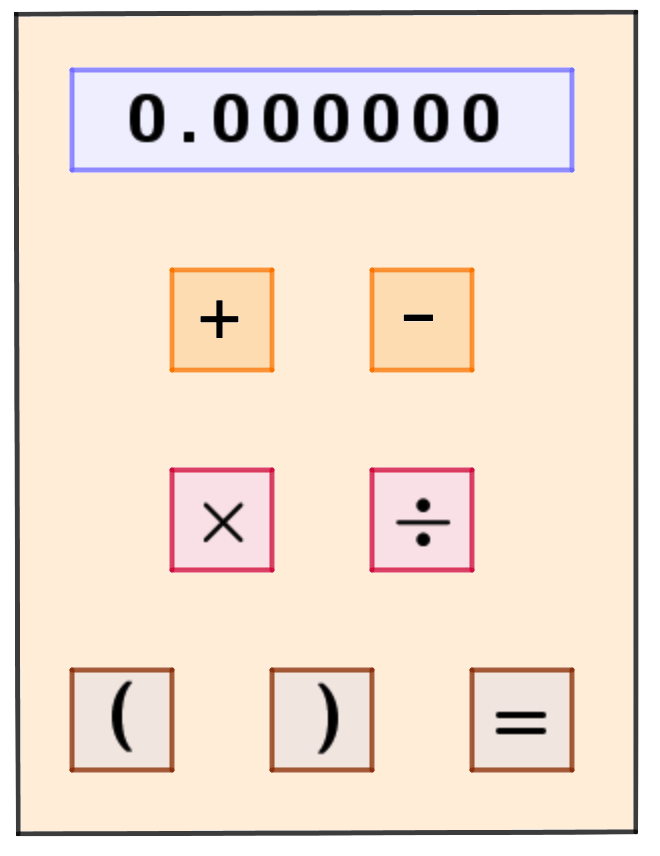
\includegraphics[width=0.35\textwidth]{img-pol/pol01.png}
\end{figure}	
\end{multicols}


El procedimiento usual sería: 

$\ p(0.82)=7.25 \times 0.82 \times 0.82 \times 0.82 - 4.02 \times 0.82 \times 0.82 + 3.19 \times 0.82 - 5.36$	

En total, 6 multiplicaciones, una suma y dos restas, total, $\ 6\times 5+ 3\times 1=33 $ \euro.

\vspace{2mm} Démosle una oportunidad a Ruffini:

\begin{multicols}{2}
\begin{table}[H]
\centering
\begin{tabular}{r|rrrr}
 & 7.25 & -4.02 & 3.19 & -5.36 \\
0.82 & $\downarrow$  & $\boldsymbol{\times}$ & $\boldsymbol{\times}$ & $\boldsymbol{\times}$ \\ \hline
 & 7.25 & $\boldsymbol{+}$ & \multicolumn{1}{r|}{$\boldsymbol{+}$} & $\boldsymbol{+}$ \\ \cline{5-5}
\end{tabular}
\end{table}	

En esta ocasión hemos usado 3 productos y 3 sumas: $\ 3\times 5 + 3\times 1 = 18 $ \euro. Es la opción más económica!
\end{multicols}

Realmente, el método de Ruffini es como sacar factor común:

$p(0.82)=\left[ \left( 7.25 \times 0.82 - 4.02 \right) \times 0.82 + 3.19 \right] \times 0.82 - 5.36 \, , \ $ 3 productos y tres sumas (restas).

\end{myexampleblock}


\vspace{1cm}
\section{Fracciones algebraicas}
\begin{tikzpicture}
	\fill [left color=red!50, right color=teal!50] (0,0) rectangle (3.5,.1);
	\fill [left color=teal!50, right color=blue!50] (3.5,0) rectangle (7.5,.1);
	\end{tikzpicture}
\vspace{0.5cm}



\begin{definition}[ MCM y MCD de polinomios]

\vspace{2mm} El máximo común divisor (MCD) de varios polinomios es el polinomio de mayor grado que es divisor común de todos ellos. 

\vspace{2mm} Para encontrar el MCM de varios polinomios se descomponen estos en factores y se toman los factores comunes elevados a la menor potencia.


\vspace{4mm} El mínimo común multiplo (MCM) de varios polinomios es el polinomio de menor grado que es múltiplo de todos ellos.

\vspace{2mm} Para encontrar el MCM de varios polinomios se descomponen estos en factores y se toman los factores comunes y no comunes elevados a la mayor potencia.
	
\end{definition}

\vspace{4mm}
\begin{miejemplo}

Encuentra el MCM y el MCD de $\ p(x)=x^6-x^2 \ $ y $ \ q(x)=x^3-x^2+x-1$

\vspace{4mm} Primero buscamos la descomposición factorial de ambos polinomios.

\vspace{2mm} $p(x)=x^2(x^4-1)=x^2(x^2-1)(x^2+1)=x^2(x-1)(x+1)(x^2+1)$

\vspace{2mm} Por Ruffin, $\ q(x)=(x-1)(x^2+1)$

\vspace{2mm} $MCD \, \left( p(x),q(x) \right)= (x-1)(x^2+1);\qquad 
MCM \, \left( p(x),q(x) \right)=x^2(x-1)(x+1)(x^2-1)$

\vspace{2mm} \textcolor{gris}{En este caso, al ser $p(x)$ múltiplo de $q(x)$, el MCD es $q(x)$ y el MCM es $p(x)$}
	
\end{miejemplo}

\begin{miejercicio}

Encuentra el MCM y el MCD de los polinomios:

$p(x)=x^2+9x+18;\qquad q(x)=x^2+6x+9;\qquad r(x)=x^2+x-6$

\rule{250pt}{0.1pt}

$p(x)=(x+6)(x+3);\qquad q(x)=(x+3)^2;\qquad r(x)=(x-2)(x+3)$	
 
\vspace{2mm} $MCM(p,q,r)=\, x+3;\qquad $

$MCM(p,q,r)=\, (x-2)(x+3)^2(x+6) \textcolor{gris}{ = x^{4} + 10 \; x^{3} + 21 \; x^{2} - 36 \; x - 108}$
\end{miejercicio}
\vspace{5mm}

\begin{definition}[ Fracción algebraica]

Una \emph{fracción algebraica} es el cociente entre dos polinomios $p(x)$ y $q(x)$, siendo el polinomio del denominador no nulo: $\quad \boldsymbol{\dfrac{p(x)}{q(x)}}$

\vspace{4mm} Al igual que las fracciones de números, dos fracciones algebraicas son \emph{equivalentes} si su producto cruzado coincide.
$\qquad \dfrac{p(x)}{q(x)} \equiv  \dfrac{r(x)}{s(x)} \ \leftrightarrow \ p(x)\cdot s(x)=q(x)\cdot r(x)$

\vspace{4mm} Para \emph{simplificar} una fracción algebraica, se descomponen numerador y denominador en factores y se suprimen los factores comunes a ambos, queda así una fracción equivalente a la original con grados de numerador y denominador menores o iguales.
	
\end{definition}

\begin{miejemplo}

Simplifica la fracción: $\qquad \dfrac{x^3-6x^2+5x+12}{2x^3-7x^2-5x+4}$

\vspace{4mm} Factorizando, por Ruffini, ambos polinomios:

\vspace{2mm} $\dfrac{x^3-6x^2+5x+12}{2x^3-7x^2-5x+4}=
\dfrac { \cancel{(x+1)} (x-3) \bcancel{(x-4)}} { \cancel{(x+1)} \bcancel{(x-4)} (2x-1) }= \dfrac{x-3}{2x-1}$
	
\end{miejemplo}


\begin{theorem}[ Operaciones con fracciones algebraicas]

\begin{itemize}
\item \textbf{Suma y resta}: se procede igual que con las fracciones numéricas, buscando el MCM de los denominadores (para lo que hay que factorizarlos previamente). Al acabar, si es posible, hay que simplificar la fracción algebraica obtenida (en sumas y restas habrá que realizar las operaciones que aparezcan en el numerador, pero el denominador se puede dejar factorizado) .
\item \textbf{Producto y división}: se procede como con las fracciones numéricas. Como al final habrá que simplificar el resultado obtenido y con vista a realizar cálculos más sencillos, es conveniente factorizar previamente las fracciones con que vamos a operar.
\end{itemize}
	
\end{theorem}

\begin{miejemplo}

Realiza la operación: $\quad \dfrac{2}{x-1}-\dfrac{x+3}{x^2-1}+\dfrac{3}{x+1}$
	
\vspace{2mm} $MCM\left( \ x-1, \ x^2-1=(x+1)(x-1),\ x+1 \ \right) \ = \ x^2-1=(x+1)(x-1)$

\vspace{2mm} $\dfrac{2}{x-1}-\dfrac{x+3}{x^2-1}+\dfrac{3}{x+1}= \dfrac
{2(x+1)-(x+3)+3(x-1)}
{(x+1)(x-1)}=
\dfrac{4x-4}{(x+1)(x-1)}= $ 

\vspace{2mm} $=\dfrac {4 \cancel{ (x-1) } }  { \cancel{(x-1)} (x+1) }= \dfrac{4}{x-1} \qquad \to \qquad \dfrac{2}{x-1}-\dfrac{x+3}{x^2-1}+\dfrac{3}{x+1} \ = \  \dfrac{4}{x-1}$
\end{miejemplo}

\begin{miejemplo}

Realiza la operación: $\quad \dfrac{x^2-4}{x^2+4x+4}\, : \, \dfrac{x^2-4x+4}{x^2+2x}$	

\vspace{2mm} Factorizando: $\quad \dfrac{x^2-4}{x^2+4x+4}\, : \, \dfrac{x^2-4x+4}{x^2+2x} = 
\dfrac{(x-2)\cancel{(x+2)}}{(x+2)^{\cancel{2}}}\, : \, \dfrac{(x-2)^2}{x(x+2)}= $

\vspace{2mm} $=\ \dfrac{\cancel{(x-2)}x\bcancel{(x+2)}}{\bcancel{(x+2)}(x-2)^{\cancel{2}}}=\dfrac{x}{x-2} \qquad \to \qquad \dfrac{x^2-4}{x^2+4x+4}\, : \, \dfrac{x^2-4x+4}{x^2+2x} \ = \ \dfrac{x}{x-2}$

\vspace{2mm} 

\vspace{2mm} 
\end{miejemplo}


\begin{figure}[H]
	\centering
	
\includegraphics[width=0.35\textwidth]{img-pol/pol05.png}
\end{figure}




%*****
\begin{miejercicio}

Simplifica: $\quad \dfrac{x^4-8x^2-9}{x^5-6x^3-6x^2-7x-6}$

\rule{250pt}{0.1pt}

\begin{multicols}{2}

$x^4-8x^2-9$

\begin{table}[H]
\centering
\begin{tabular}{r|rrrrr}
 & 1 & 0 & -8 & 0 & -9 \\
3 &  & 3 & 9 & 3 & 9 \\ \hline
 & 1 & 3 & 1 & \multicolumn{1}{r|}{3} & 0 \\ \cline{6-6} 
-3 &  & -3 & 0 & -3 &  \\ \cline{1-5}
 & 1 & 0 & \multicolumn{1}{r|}{1} & 0 &  \\ \cline{5-5}
\end{tabular}
\end{table}

$\nexists x\in \mathbb R \ / \ x^2+1=0$

$(x-3)(x+3)(x^2+1)$

$\qquad$

$\qquad$ %%%%%%

$x^5-6x^3-6x^2-7x-6$

\begin{table}[H]
\centering
\begin{tabular}{r|rrrrrr}
 & 1 & 0 & -6 & -6 & -6 & -6 \\
-1 &  & -1 & 1 & 5 & 1 & 6 \\ \hline
 & 1 & -1 & -5 & -1 & \multicolumn{1}{r|}{-6} & 0 \\ \cline{7-7} 
-2 &  & -2 & 6 & -2 & 6 &  \\ \cline{1-6}
 & 1 & -3 & 1 & \multicolumn{1}{r|}{-3} & 0 &  \\ \cline{6-6}
3 &  & 3 & 0 & 3 &  &  \\ \cline{1-5}
 & 1 & 0 & \multicolumn{1}{r|}{1} & 0 &  &  \\ \cline{5-5}
\end{tabular}
\end{table}

$\nexists x\in \mathbb R \ / \ x^2+1=0$

$(x+1)(x+2)(x-3)(x^2+1)$

\end{multicols}

\vspace{2mm}$\dfrac{x^4-8x^2-9}{x^5-6x^3-6x^2-7x-6}	=\dfrac{(x^2+1)(x+3)(x-3)}{(x^2+1)(x+1)(x+2)(x-3)}=\dfrac{x+3}{(x+2)(x+1)}$
\end{miejercicio}


%*****
\begin{miejercicio}

Calcula: $\quad \dfrac{3x-2}{x^2+x}+\dfrac{4}{x^2-x-2}$

\rule{250pt}{0.1pt}

La factorización de los denominadores es sencilla, 

$\ x^2+x=x(x+1)\ \ $ y $\ \ x^2-x-2=(x+1)(x-2) \quad \to \quad MCM=x(x+1)(x-2)$ 

\vspace{3mm}  $\dfrac{3x-2}{x^2+x}+\dfrac{4}{x^2-x-2}= \dfrac{3x-2}{x(x+1)}+\dfrac{4}{(x+1)(x-2)}=\dfrac{(3x-2)(x-2)+4\, x}{x(x+1)(x-2)}=\dfrac{3x^2-8x+4+4x}{x(x+1)(x+2)}=\dfrac{3x^2-4x+4}{x(x+1)(x+2)}$

\vspace{3mm} Al factorizar el numerador para ver si podemos simplificar, vemos que se trata de un polinomio irreducible. Hemos acabado (no es necesario desarrollar las operaciones que aparecen en el denominador, es mejor dejarlo factorizado).
	
\end{miejercicio}


%*****
\begin{miejercicio}

Calcula: $\quad \left( \dfrac{2x}{x-5}\, : \, \dfrac{3x^2}{x^2-25} \right) \, : \, \dfrac{2x+10}{x}$

\rule{250pt}{0.1pt}

Todos los polinomios que aparecen son fácilmente factorizables: $\ x^2-25=(x-5)(x+5)\ $ y $\ 2x+10=2(x+5)\, , \ $ en este último caso tenemos un polinomio de primer grado que, aún siendo irreducible, es susceptible de sacar factor común (un 2, en este caso).

\vspace{3mm} 
$ \left( \dfrac{2x}{x-5}\, : \, \dfrac{3x^2}{x^2-25} \right) \, : \, \dfrac{2x+10}{x}= \left( \dfrac{2x}{x-5} \, : \, \dfrac{3x^2}{(x-5)(x+5)} \right) \, : \, \dfrac{2(x+5)}{x}= $

\vspace{2mm} $=\dfrac{2\bcancel{x}\cancel{(x-5)}(x+5)}{\cancel{(x-5)}\, 3x^{\bcancel{2}}}\, : \,  \dfrac{2(x+5)}{x}= \dfrac{2(x+5)}{3x}\, : \,  \dfrac{2(x+5)}{x} = \dfrac{\cancel{2}\cancel{(x+5)}\cancel{x}}{3\cancel{x}\, \cancel{2}\cancel{(x+5)}}= \dfrac 1 3$
	
\end{miejercicio}


%*****
\begin{miejercicio}

Calcula: $\quad \left( 4-\dfrac{3x^2}{x^2-1}\right) \cdot \dfrac{x+1}{x^2-4}$

\rule{250pt}{0.1pt}

\vspace{2mm} $\left( 4-\dfrac{3x^2}{x^2-1}\right) \cdot \dfrac{x+1}{x^2-4}=
\left( 	\dfrac 4 1-\dfrac{3x^2}{(x+1)(x-1)}\right) \cdot \dfrac{x+1}{(x+2)(x-2)}=$

\vspace{2mm}
$\dfrac{4(x+1)(x-1)-3x^2}{(x+1)(x-1)} \cdot \dfrac{x+1}{(x+2)(x-2)}=
\dfrac{4x^2-4-3x^2}{(x+1)(x-1)} \cdot \dfrac{x+1}{(x+2)(x-2)}=$

\vspace{2mm} 
$\dfrac{x^2-4}{(x+1)(x-1)} \cdot \dfrac{x+1}{(x+2)(x-2)}=
\dfrac{(x+2)(x-2)}{(x+1)(x-1)} \cdot \dfrac{x+1}{(x+2)(x-2)}=$

\vspace{2mm}
$\dfrac{(x+2)(x-2)(x+1)}{(x+1)(x-1)(x+2)(x-2)} = \dfrac {1}{x-1}$
	
\end{miejercicio}


%*****
\begin{miejercicio}

Calcula: $\quad \left( \dfrac{x}{x^2-3x-4}-\dfrac{2x}{x^2-1}+\dfrac{x^2-6x-4}{x^3-4x^2-x+4} \right) \cdot (x^2-1)$

\rule{250pt}{0.1pt}

Denominadores: 

\vspace{2mm}$\begin{cases}\  x^2-3x-4=(x+1)(x-4) \\ \ 	x^2-1=(x-1)(x+1)\\ \ x^3-4x^2-x+4=(x-1)(x+1)(x-4) \end{cases} \ \to \ \ MCM=\ (x-1)(x+1)(x-4)$

\vspace{4mm}
 $\left( \dfrac{x}{x^2-3x-4}-\dfrac{2x}{x^2-1}+\dfrac{x^2-6x-4}{x^3-4x^2-x+4} \right) \cdot (x^2-1) = $
 
 \vspace{2mm}\begin{small} $= \dfrac{x(x-1)-2x(x-4)+x^2-6x-4}{(x-1)(x+1)(x-4)}  \cdot (x^2-1)= \dfrac{x^2-x-2x^2+8x+x^2-6x-4}{(x-1)(x+1)(x-4)}\cdot (x^2-1)=$ \end{small}
 
 \vspace{2mm} $= \dfrac{x-4}{(x-1)(x+1)(x-4)}\cdot (x^2-1)=\dfrac{1}{(x+1)(x-1)}\cdot (x^2+1)= \dfrac{x^2+1}{(x-1)(x+1)}= 1$	
\end{miejercicio}



%%%%%%%%%%%%%%%%%%%%%%%%%%%%%%%

\section{Ejercicios}
\begin{tikzpicture}
	\fill [left color=red!50, right color=teal!50] (0,0) rectangle (3.5,.1);
	\fill [left color=teal!50, right color=blue!50] (3.5,0) rectangle (7.5,.1);
	\end{tikzpicture}
\vspace{0.5cm}

%************
\begin{mipropuesto}

Calcula: $\quad \left( \, \frac 1 4 x^4+\frac 1 2 x^3+x^2+\frac 5 2 x -\frac 5 4 \, \right) \, : \, \left(\, \frac 1 2 x^2+x-\frac 1 2 \, \right)$
\end{mipropuesto}

\vspace{-8mm}
\begin{flushright}
	\begin{footnotesize} \textcolor{gris}{\rotatebox{180}{ $c(x)= \frac 1 2 x^2 + \frac 5 2 ;\quad r(x)= 0$ }}	\end{footnotesize}
\end{flushright}

%************
\begin{mipropuesto}

Calcula: $\quad \left( \, x^4-\frac 1 2 x^2+\frac 1 3 \, \right) º, : \, \left( \, x+\frac 1 2 \, \right)$ 
\end{mipropuesto}

\vspace{-8mm}
\begin{flushright}
	\begin{footnotesize} \textcolor{gris}{\rotatebox{180}{ $c(x)=x^3-1/2\, x^2-1/4\, x+1/8;\quad r(x)=13/48$ }}	\end{footnotesize}
\end{flushright}


%************
\begin{mipropuesto}

Encontrar el valor de $k$ para que el resto de la división $(x^3-7x^2+3x+k)\, : \, (x^2-x+2)\, $ sea $\, -5x+2$
\end{mipropuesto}

\vspace{-8mm}
\begin{flushright}
	\begin{footnotesize} \textcolor{gris}{\rotatebox{180}{ $k=-10$ }}	\end{footnotesize}
\end{flushright}

%************
\begin{mipropuesto}

Encuentre el valor de $m$ y $n$ para que el resto de la división $(x^4+2x^3+mx+n)\, :\, (x^2+3x-1)$ sea $2x+1$
\end{mipropuesto}

\vspace{-8mm}
\begin{flushright}
	\begin{footnotesize} \textcolor{gris}{\rotatebox{180}{ $m=15,\ \ \ n=-3$ }}	\end{footnotesize}
\end{flushright}


%************
\begin{mipropuesto}

Encuentra el valor de $t$ para que el cociente de la división $(2x^3+\, t \, x^2+6x+1)\, : \, (x^2+5x)$ sea un monomio.
\end{mipropuesto}

\vspace{-8mm}
\begin{flushright}
	\begin{footnotesize} \textcolor{gris}{\rotatebox{180}{ $t=10$ }}	\end{footnotesize}
\end{flushright}



%************
\begin{mipropuesto}

Encuentra el valor de $k$ para que el valor numérico de $p(x)=x^5-x^4+x+3k)$ en $x=2$ sea $5$. ?`Cuál es el resto de dividir $p(x)$ entre $(x-2)$?
\end{mipropuesto}

\vspace{-8mm}
\begin{flushright}
	\begin{footnotesize} \textcolor{gris}{\rotatebox{180}{ $k=-13/3;\ \ \ r(x)=5$ }}	\end{footnotesize}
\end{flushright}


%************
\begin{mipropuesto}

Encuentra los valores de $m$ y $n$ para que $p(x)=x^3-5x^2+mx+n$ sea divisible, a la vez, por $x+1$ y por $x-1$
\end{mipropuesto}

\vspace{-8mm}
\begin{flushright}
	\begin{footnotesize} \textcolor{gris}{\rotatebox{180}{ Sistema dos ecuaciones lineales con dos incógnitas, $\ \ m=-1,\ n=5$ }}	\end{footnotesize}
\end{flushright}

%************
\begin{mipropuesto}

Facroriza los siguientes polinomios:

\begin{multicols}{2}
\begin{enumerate}[a) ]
\item $\ 6x^2-19x-7$
\item $\ x^3+2x^2-20x-40$
\item $\ (4m-2n)x^4-(4m-2n)	$
\item $\ x^5-5x^4+10x^3-10x^2+5x-1$
\end{enumerate}	
\end{multicols}


\end{mipropuesto}



\vspace{-8mm}
\begin{flushright}
	\begin{footnotesize} \textcolor{gris}{\rotatebox{180}{ $a)\ (2x-7)(3x+1);\quad b)\ (x-2)(x+\sqrt{20})(x-\sqrt{20});\quad c)\ 2(2m-n)(x-1)(x+1)(x^2+1);\quad d)\ (x-1)^5$  }}	\end{footnotesize}
\end{flushright}

%************
\begin{mipropuesto}

Sabiendo que $2/5$ es una raíz de $p(x)=20x^3+52x^2+21x-18$, descomponerlo en factores.
\end{mipropuesto}

\vspace{-8mm}
\begin{flushright}
	\begin{footnotesize} \textcolor{gris}{\rotatebox{180}{ Ruffini y ecuación de segundo grado: $\ \ (5x-2)(2x+3)^2$ }}	\end{footnotesize}
\end{flushright}


%************
\begin{mipropuesto}

Encuentra el valor de $a$ y $b$ sabiendo que las siguientes fracciones algebraicas son equivalentes:
$\qquad  \dfrac{x^2-3x-10}{x^2+5x+a};\qquad \dfrac{x-b}{x+3}$
\end{mipropuesto}

\vspace{-8mm}
\begin{flushright}
	\begin{footnotesize} \textcolor{gris}{\rotatebox{180}{ $a=6;\ \ b=5$ }}	\end{footnotesize}
\end{flushright}

%************
\begin{mipropuesto}

Simplifica las siguientes fracciones algebraicas:

\begin{multicols}{2}
\begin{enumerate}[a) ]
\item $\dfrac{x^2+3x-4}{x^2+4x}$
\item $\dfrac{2x^3-2}{x^3-x^2-x-2}$
\item $\dfrac{x^4-2x^3+x^2-2x}{x^2-4}$
\item $\dfrac{x^5-x^2}{x^4+x^3+x^2}$	
\end{enumerate}	
\end{multicols}
\vspace{1mm}
\end{mipropuesto}

\vspace{-8mm}
\begin{flushright}
	\begin{footnotesize} \textcolor{gris}{\rotatebox{180}{ $a)\ \dfrac{x-1}{x};\quad b)\ \ \dfrac{2x-2}{x-2};\quad c)\ \ \dfrac{x^3+x}{x+2};\quad d)\ \ x-1 $ }}	\end{footnotesize}
\end{flushright}

%************
\begin{mipropuesto}

Escribe una fracción de numerador $\, 20x-5\, $ que sea equivalente a $\dfrac{5}{3x+1}$
\end{mipropuesto}

\vspace{-8mm}
\begin{flushright}
	\begin{footnotesize} \textcolor{gris}{\rotatebox{180}{ $\dfrac{20x-5}{12x^2+x-1}$ }}	\end{footnotesize}
\end{flushright}


%************
\begin{mipropuesto}

Realiza las siguientes operaciones:

\begin{multicols}{2}
\begin{enumerate}[a) ]
\item $\dfrac{1-x^2}{x^2-4x}+\dfrac{3x-x^2}{4x-x^2}+\dfrac{x^2-x-1}{x^2-4x}$
\item $\dfrac{x-4}{x+2}+\dfrac{x-1}{x+3}$
\item $\dfrac{x-2}{x-1}+\dfrac{x-1}{x+1}$
\item $\dfrac{1}{2x-4}+\dfrac{x-3}{x+2}+\dfrac{x-x^2}{x^2-4}$	
\item $\dfrac{3}{x+3}-\dfrac{1}{x+2}-\dfrac{x}{x^2+5x+6}$
\item $\dfrac{x-1}{x-3}+\dfrac{x+4}{x+2}-\dfrac{2x^2+3x-12}{x^2-x-6}$
\end{enumerate}	
\end{multicols}
\vspace{1mm}
\end{mipropuesto}

\vspace{-8mm}
\begin{flushright}
	\begin{footnotesize} \textcolor{gris}{\rotatebox{180}{ $a)\ -1;\ \ \ b)\ \dfrac{2x^2-14}{x^2+5x+6};\ \ \ c)\ \dfrac{2x^2-3x-1}{x^2-1}; \ \ \ d)\ \dfrac{x-10}{2x^2-8};\ \ \ e)\ \dfrac{1}{x+2};\ \ \ f)\ \dfrac{1}{3-x}$ }}	\end{footnotesize}
\end{flushright}

%************
\begin{mipropuesto}

Realiza las siguientes operaciones:

\begin{multicols}{2}
\begin{enumerate}[a) ]
\item $\dfrac{x^2+2x+1}{x-3}\cdot \dfrac{x^2+x-12}{x^2-1}$
\item $\dfrac{x^2-2x-3}{x^2-5x}\cdot \dfrac{x^2-4x-5}{x^2-4x+3}$
\item $\dfrac{x+2}{x^2+4x+4}\, : \, \dfrac{x^2-4}{x^3+8}$
\item $\left( \dfrac{x+5}{x-3} -1\right)\cdot \left( \dfrac{4-x}{x-2}+1\right)$
\end{enumerate}	
\end{multicols}
\vspace{1mm}	
\end{mipropuesto}

\vspace{-8mm}
\begin{flushright}
	\begin{footnotesize} \textcolor{gris}{\rotatebox{180}{ $a)\ \dfrac{x^2+5x+4}{x-1};\ \ \ b)\ \dfrac{x*2+2x+1}{x^2-x};\ \ \ c)\ \dfrac{x^2-2x+4}{x^2-4};\ \ \ d)\ \dfrac{16}{x^2-5x+6}$ }}	\end{footnotesize}
\end{flushright}

%************
\begin{mipropuesto}

Calcula:
$\qquad \left( \, x+1\, + \, \dfrac{x^3}{x-x^2} \, \right) \, : \, \left( \, 1\, -\, \dfrac{1}{x+1} \cdot \dfrac{2x}{1-x^2} \, \right)$
\end{mipropuesto}

\vspace{-8mm}
\begin{flushright}
	\begin{footnotesize} \textcolor{gris}{\rotatebox{180}{ Simplifica a medida que calculas $\quad \dfrac{1}{2-x}$ }}	\end{footnotesize}
\end{flushright}


%************
\begin{mipropuesto}

Calcula: $\qquad a)\ \ \dfrac{x-\dfrac{x}{x+1}}{x+\dfrac{x}{x-1}} \, ; \qquad \qquad b)\ \ \dfrac{1-\dfrac{1+x^2}{1-x^2}}{1+\dfrac{1+x^2}{1-x^2}}$
\end{mipropuesto}

\vspace{-8mm}
\begin{flushright}
	\begin{footnotesize} \textcolor{gris}{\rotatebox{180}{ $a)\ \dfrac{x-1}{x+1};\ \ \ b)\ -x^2$ }}	\end{footnotesize}
\end{flushright}

%%%%%%%%%%%%%%%%%%%%%%%%%%%%%%%%%%%%


\newpage

$\quad$

$\quad$


\begin{adjustwidth}{50pt}{250pt}
\begin{cuadro-naranja}
\textbf{\huge{Problemas $\boldsymbol{+}$}}\normalsize{$\, $}
\end{cuadro-naranja}	
\end{adjustwidth}

\vspace{5mm}
\begin{enumerate}[\textbf{P$\boldsymbol +$} 1. ]
\item	Factoriza el polinomio: $\ \ (x+3)^3-(x+2)^3-(x+1)^3-x^3$

\vspace{-6mm}
\begin{flushright}
\begin{footnotesize} \textcolor{gris}{\rotatebox{180}{ $2(x-3)(x^2+3x+3)$ }}	\end{footnotesize}
\end{flushright}


\item	Si $6$ es raíz de $p(x)=x^2-2x+1$, ?`cuál es el valor de $a$?

\vspace{-6mm}
\begin{flushright}
\begin{footnotesize} \textcolor{gris}{\rotatebox{180}{ -4 }}	\end{footnotesize}
\end{flushright}


\item	$x^2-n^2x+2n$ tiene dos raíces distintas, si una es $n=2$, ?`cuál es la otra?

\vspace{-6mm}
\begin{flushright}
\begin{footnotesize} \textcolor{gris}{\rotatebox{180}{ -1 }}	\end{footnotesize}
\end{flushright}

%
\item	Sea un polinomio tal que $\ p(x^2+1)= x^4+4x^2\, , \ $ determina $p(x^2-1)$

\vspace{-6mm}
\begin{flushright}
\begin{footnotesize} \textcolor{gris}{\rotatebox{180}{a la hipótesis ($x^4+4x^2$). Identifica coeficientes. Luego, calcula $p(x^2-1$. $\quad$ sol: $p(x^2-1)=x^4-4$}}	\end{footnotesize}
\end{flushright}
\vspace{-8mm}
\begin{flushright}
\begin{footnotesize} \textcolor{gris}{\rotatebox{180}{ $p(x)$ ha de ser un polinomio de segundo grado, $p(x)=ax^2+bx+c$. Calcula $p(x^2+1)$ e iguala  }}	\end{footnotesize}
\end{flushright}


%
\item	Al dividir $p(x)$ entre $(x-1)$ el resto es $-8$, si lo dividimos por $(x+2)$ el resto es $25$. ?`Cuál es el resto de dividir a $p(x)$ entre $x^2+x-2\,$?

\vspace{-6mm}
\begin{flushright}
\begin{footnotesize} \textcolor{gris}{\rotatebox{180}{ $p(1)=-8;\ p(-2)=25;\ x^2+x-2=(x-1)(x+2)$  El resto de dividir $p(x)$ por $x^2+x-2$ será }}	\end{footnotesize}
\end{flushright}
\vspace{-8mm}
\begin{flushright}
\begin{footnotesize} \textcolor{gris}{\rotatebox{180}{un polinomio de primer grado, $mx+n$, luego $p(x)=c(x)(x-1)(x+2)+(mx+n)$ }}	\end{footnotesize}
\end{flushright}
\vspace{-8mm}
\begin{flushright}
\begin{footnotesize} \textcolor{gris}{\rotatebox{180}{ Impón tus condiciones y la solución es: $\ -11x+3$}}	\end{footnotesize}
\end{flushright}
 
\end{enumerate}



%%%%%%%%%%%%%%%%%%%%%%%%%%%%%%%%%%%%
\newpage
\section{Resumen del tema}
\begin{tikzpicture}
	\fill [left color=red!50, right color=teal!50] (0,0) rectangle (3.5,.1);
	\fill [left color=teal!50, right color=blue!50] (3.5,0) rectangle (7.5,.1);
	\end{tikzpicture}
\vspace{1cm}


\begin{myblock}{Resumen: \emph{``Polinomios y fracciones algebraicas''}}

\underline{Teorema del resto}:  $a$ es raíz de $p(x)$ si $p(a)=0 \ \Rightarrow \ p(x) $ es divisible por $\ x-a$ .

\vspace{2mm}
--- Los polinomios de primer grado son irreducibles.

--- Los polinomios de segundo grado con soluciones reales $x_1$ y $x_2$ se pueden factorizar como $a(x-x_1)(x-x_2)\, . \ $ Si no hay soluciones reales, el polinomio es primo.

\vspace{5mm} Si $p(x)$ tiene coeficientes enteros $\ \Rightarrow $

\begin{itemize}
\item Candidatos a raíces enteras: 	$\ \pm $ divisores del término independiente.
\item Candidatos a raíces racionales: 	$\ \pm $ divisores del término independiente, dividido por divisores del término dominante.
\end{itemize}


\vspace{3mm}
\begin{small}
Si el polinomio tiene coeficientes enteros, el \textbf{procedimiento} a seguir para factorizarlo será el siguiente:

\begin{enumerate}
\vspace{-2mm}\item Encontramos los divisores del término independiente. Si no tuviese término independiente sacaríamos factor común y seguiríamos intentando factorizar el resultado.

\vspace{-2mm}\item Comprobamos si son raíces del polinomio, comenzando
por el más pequeño.

\vspace{-2mm}\item Con el primero que encontremos aplicamos la regla de
Ruffini.

\vspace{-2mm}\item Tomamos el cociente que hayamos obtenido y
repetimos el proceso empezando a probar con la misma
raíz obtenida anteriormente.

\vspace{-2mm}\item Si un divisor del término independiente no es raíz en un
paso, tampoco lo será en el siguiente. Puede que haya raíces repetidas (dobles, triples, etc.); por lo tanto, si una raíz lo es en un paso, también lo puede ser en el siguiente.

\vspace{-2mm}\item Cuando tengamos un cociente de grado 2, podemos resolver la ecuación correspondiente de 2o grado. Es la única opción que tenemos si el polinomio tiene raíces reales no enteras (racionales o irracionales). 

$ax^2+bx+c=0 \to x=x_1 \vee x=x_2 \ \Rightarrow \ \boldsymbol{ax^2+bx+c=a(x-x_1)(x-x_2)}$

\vspace{-2mm}\item Finalmente escribimos la descomposición en producto de factores del polinomio.
\end{enumerate}
El \emph{teorema fundamental del álgebra} asegura que un polinomio de grado $n$ tiene, a lo sumo, $n$ raíces reales.

También se pueden usar los \emph{productos notables} para la factorización de polinomios. 
\end{small}	
\end{myblock}





\begin{comment}
%%%%%%%%%%%%%%%%%%%%%%%%%%%%%%%%%%%. SECCIONES
\begin{figure}[H]
	\centering
	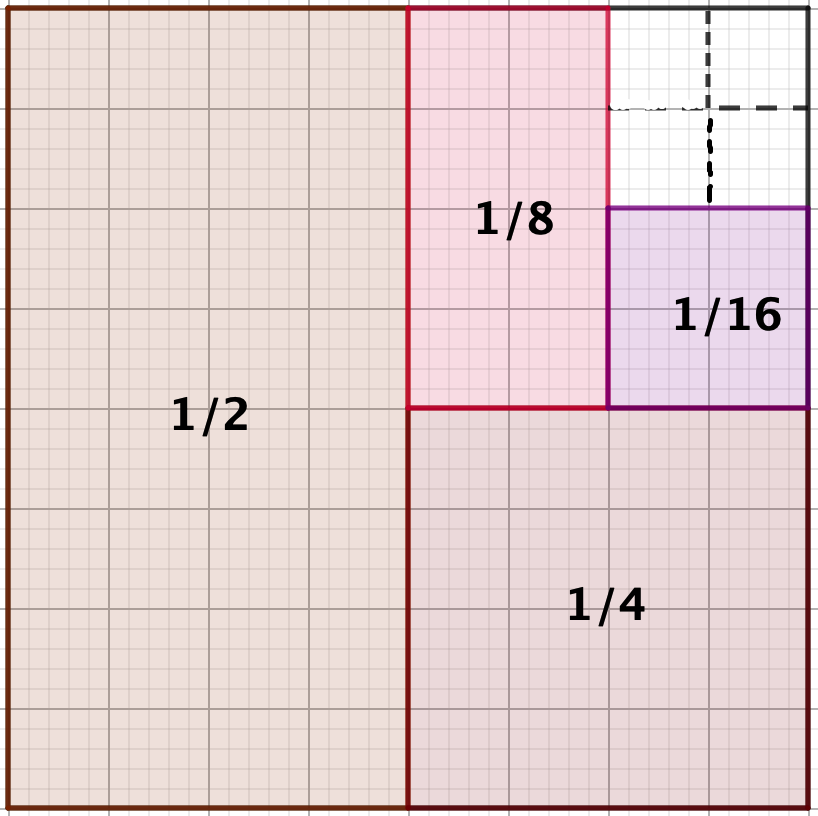
\includegraphics[width=0.25\textwidth]{img-suc/suc03.png}
\end{figure}



\chapter{texto}
\begin{tikzpicture}
	\fill [left color=red!50, right color=teal!50] (0,0) rectangle (6.5,.2);
	\fill [left color=teal!50, right color=blue!50] (6.5,0) rectangle (11.5,.2);
	\end{tikzpicture}

\vspace{1cm}
\section{texto}
\begin{tikzpicture}
	\fill [left color=red!50, right color=teal!50] (0,0) rectangle (3.5,.1);
	\fill [left color=teal!50, right color=blue!50] (3.5,0) rectangle (7.5,.1);
	\end{tikzpicture}
\vspace{0.5cm}

\subsection{texto}
\begin{tikzpicture}
	\fill [left color=red!50, right color=teal!50] (0,0) rectangle (3.5,.01);
	\fill [left color=teal!50, right color=blue!50] (3.5,0) rectangle (7.5,.01);
	\end{tikzpicture}
\vspace{0.5cm}


%%%%%%%%%%%%%%%%%%%%%%%%%%%%%%%%%%%. \begin{ ------>. 
detsacado;  cuadro-naranja;  cuadro-gris;  miejercicio (solución extensa);  mipropuesto (solución corta y fuera del cuadro) \theomen  \definition

%%%%%%%%%%%%%%%%%%%%%%%%%%%%%%%%%%%. CURIOSIDAD
\vspace{1cm}
\color{ForestGreen!80}
\rule{250pt}{0.2pt}
Texto
\vspace{-8mm}
\begin{flushright}
\rule{250pt}{0.2pt}		
\end{flushright}	
\color{black}
\end{comment} %
\chapter{Ecuaciones y sistemas}
\begin{tikzpicture}
	\fill [left color=red!50, right color=teal!50] (0,0) rectangle (6.5,.2);
	\fill [left color=teal!50, right color=blue!50] (6.5,0) rectangle (11.5,.2);
	\end{tikzpicture}


\vspace{10mm}
\begin{adjustwidth}{40pt}{40pt}
\begin{cuadro-gris}

	\begin{multicols}{2}
	$\triangleright \ $  Ecuaciones: 
	polinómicas, racionales, radicales, exponenciales, logarítmicas, con valor absoluto.
	
	$\triangleright \ $  Sistemas de ecuaciones: 
	lineales y no lineales
	\end{multicols}
\end{cuadro-gris}
\end{adjustwidth}


\vspace{1cm}
\section{Ecuaciones polinómicas}
\begin{tikzpicture}
	\fill [left color=red!50, right color=teal!50] (0,0) rectangle (3.5,.1);
	\fill [left color=teal!50, right color=blue!50] (3.5,0) rectangle (7.5,.1);
	\end{tikzpicture}
\vspace{0.5cm}


Una \textbf{ecuación} es una igualdad matemática entre dos expresiones, denominadas miembros y separadas por el signo igual, en las que aparecen elementos conocidos, \emph{datos}, y  desconocidos, \emph{incógnitas}, relacionados mediante operaciones matemáticas. No confundir con \emph{identidad}, una igualdad algebraica que es cierta para cualquier valor de la incógnita.

\subsection{Ecuaciones de primer grado}
\begin{tikzpicture}
	\fill [left color=red!50, right color=teal!50] (0,0) rectangle (3.5,.01);
	\fill [left color=teal!50, right color=blue!50] (3.5,0) rectangle (7.5,.01);
	\end{tikzpicture}
\vspace{0.5cm}

\begin{definition}[ Ecuación de primer grado]
. Las ecuaciones de primer grado, que también se llaman ecuaciones  lineales, son de la forma: $\quad ax + b =0 \, , \ $
donde   $x$   está elevada al exponente $1$, el coeficiente   $a$   debe ser distinto de cero y el término independiente   $b$   es un número cualquiera.
\end{definition}

\begin{theorem}[ Resolución ecuación de primer grado]
. Para resolver la ecuación   $ax + b = 0$   basta con despejar la $x$ así:

$$\quad ax + b = 0   \quad \leftrightarrow \quad    ax = - b   \quad \leftrightarrow \quad  x = -b/a$$
\end{theorem}
Con frecuencia, la ecuación aparecerá con más términos. Para resolverla se realizan las siguientes transformaciones para llegar a su forma general:
\vspace{-2mm} 
\begin{multicols}{2}
\begin{enumerate}
\vspace{-2mm} \item Quitar paréntesis.
\vspace{-2mm} \item Quitar denominadores, para ello se multiplicará toda la ecuación por el MCM de los denominadores.
\vspace{-2mm} \item Agrupar los términos en $x$ en un miembro y los términos independientes (sin $x$) en el otro.

\vspace{-2mm} \item Agrupar términos semejantes.
\vspace{-2mm} \item Despejar la incógnita.
\end{enumerate}

\begin{figure}[H]
	\centering
	
\includegraphics[width=0.4\textwidth]{img-ecc/ecc01.png}
\end{figure}
\end{multicols}

\begin{destacado}
Las ecuaciones de primer grado siempre tendrán solución única, o infinitas soluciones o carecerán de solución alguna.
\end{destacado}


\begin{table}[H]
\centering
\begin{tabular}{|cc|}
\hline
\multicolumn{2}{|c|}{\textbf{Soluciones ecuación primer grado: $\quad \boldsymbol{ax=b}$}} \\ \hline
\multicolumn{1}{|c|}{$a \neq 0$} & \begin{tabular}[c]{@{}c@{}}Ecuación determinada.\\ $x=\dfrac b a$ \\ Solución única \end{tabular} \\ \hline
\multicolumn{1}{|c|}{$a=0, \ \ b=0$} & \begin{tabular}[c]{@{}c@{}} Ecuación indeterminada.\\ $0\cdot x=0 \to \forall x \in \mathbb R$ \\ Infinitas soluciones. \end{tabular} \\ \hline
\multicolumn{1}{|c|}{$a=0,\ \ b\neq 0$} & \begin{tabular}[c]{@{}c@{}}Ecuación incompatible.\\ $0\cdot x=b\neq 0 \to \nexists x$ \\  Sin solución. \end{tabular} \\ \hline
\end{tabular}
\end{table}



\begin{miejemplo}

\begin{footnotesize}
$$\dfrac{3x-2}{6}-\dfrac{3[x-3(x-2)]}{4}=x-2\left[ \dfrac{x+2}{3}-3\left( x-\dfrac{x+1}{4} \right) \right]$$


\vspace{5mm} $ QP:\qquad \dfrac{3x-2}{6}-\dfrac{3x-9(x-2)}{4}=x-\dfrac{2(x+2)}{3}+6\left( x-\dfrac{x+1}{4} \right)$

\vspace{2mm} $QP:\qquad \dfrac{3x-2}{6}-\dfrac{-6x+18}{4}=x-\dfrac{2x+4}{3}+6 x-\dfrac{3(x+1)}{2} $

\vspace{2mm} $QD:\qquad 12\cdot \dfrac{3x-2}{6}-12\cdot \dfrac{-6x+18}{4}=12\cdot 7x-12\cdot \dfrac{2x+4}{3}-12\cdot \dfrac{3x+3}{2}\ \ $ \begin{tiny} ${MCM(6,4,3,2)=12}$\end{tiny}

\vspace{2mm} $QD:\qquad 2(3x-2)-3(-6x+18)=84x-4(2x+4)-6(3x+3)$

\vspace{2mm} $QP:\qquad 6x-4+18x-54=84x-8x-16-18x-18$

\vspace{2mm} $AT:\qquad 6x+18x-84x+8x+18x=-16-18+4+54$

\vspace{2mm} $D:\qquad -34x=24 \ \to \ x=-\dfrac{24}{34}=-\dfrac{12}{17}$
\end{footnotesize}	
\end{miejemplo}

%%%%%%%%%%%%%
\begin{myexampleblock}{Epitafio de Diofanto}

\begin{figure}[H]
	\centering
	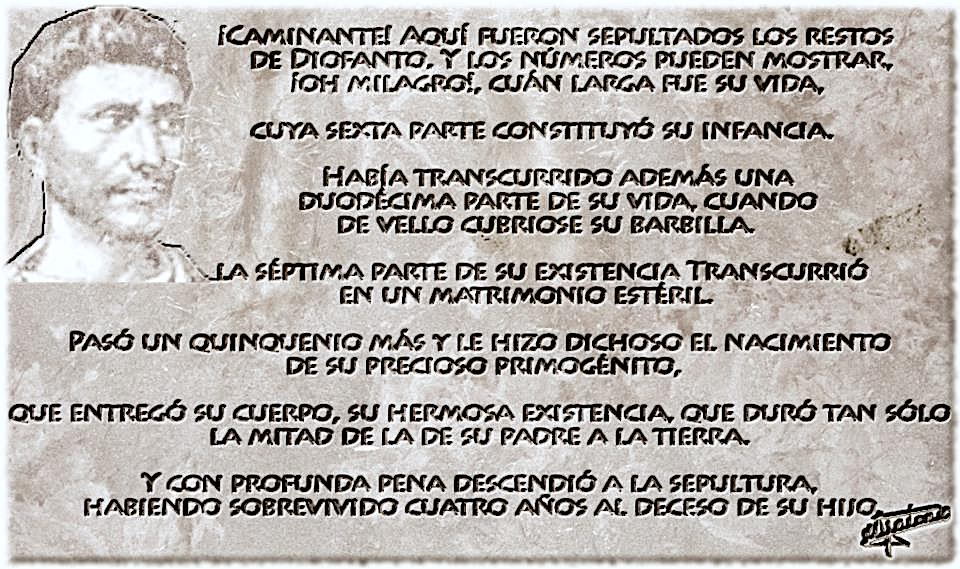
\includegraphics[width=1\textwidth]{img-ecc/ecc09.jpeg}
	\caption*{\scriptsize{Exposiciones Eureka: $\ \ $ https://www.facebook.com/Exposiciones-Eureka-484780888274874/}}
\end{figure}
	
\end{myexampleblock}




\vspace{5mm}
\subsection{Ecuaciones de segundo grado}
\begin{tikzpicture}
	\fill [left color=red!50, right color=teal!50] (0,0) rectangle (3.5,.01);
	\fill [left color=teal!50, right color=blue!50] (3.5,0) rectangle (7.5,.01);
	\end{tikzpicture}
\vspace{0.5cm}

\begin{definition}[ Ecuación de segundo grado]
. Una ecuación de segundo grado con una incógnita es una igualdad algebraica que se puede expresar de la forma: $\quad ax2 + bx + c = 0 $                     siendo $a$, $b$ y $c$ números reales y  $a \neq 0$.
\end{definition}


Si  $b$ y $c$  son números distintos de cero, se dice que la ecuación es completa. Se resuelve por el método general.

Si  $b = 0  \ \vee \   c = 0$ , la ecuación se denomina incompleta. Aunque se pueden resolver por el método general es más sencillo sacar factor común o despejar (ver ejemplo siguiente).


\begin{theorem}[ Resolución de la ecuación de segundo grado. Método general]

$$ax^2+bx+c=0\, , \ a\neq 0 \qquad \Rightarrow \qquad 
\boxed{ \ \boldsymbol{ x\ =\ \dfrac{-b\pm \sqrt{\, b^2\, -\, 4ac \, }}{2a} } \ }$$	
\end{theorem}

\underline{Demostración}: se basa en completar un cuadrado.

$ax^2+bx+c=0 \to a\left(x^2+\dfrac b a x+\dfrac c a \right)=0\, , \  $ como $a\neq 0 \to$

$\to x^2+\dfrac b a x+\dfrac c a=0 \ \to \underbrace{\left( x+\dfrac{b}{2a} \right)^2 }_{x^2+2x\dfrac{b}{2a}+\dfrac{b^2}{4a^2}}-\dfrac{b^2}{4a^2}+\dfrac c a = 0 \to \left( x+\dfrac {b}{2a} \right)^2 = \dfrac{b^2}{4a^2}-\dfrac{c}{a} = \dfrac{b^2-4ac}{4a^2}$ 

Sacando raíz cuadrada: $\ \ \left| x+\dfrac {b}{2a}\right|=\sqrt{ \dfrac{b^2-4ac}{4a^2} } \ \to \ x+\dfrac {b}{2a}=\pm \dfrac{\sqrt{ b^2-4ac }}{2a} $

Despejando $\ \ x=-\dfrac{b}{2a}\pm \dfrac{\sqrt{ b^2-4ac }}{2a}=\dfrac{-b\pm \sqrt{b^2-4ac}}{2a}$ \QED

\vspace{5mm} 

\begin{multicols}{2}
\begin{adjustwidth}{10pt}{40pt}

\begin{destacado}
Las ecuaciones de segundo grado siempre tendrán dos soluciones, una sola (que será doble) o carecerán de ellas (ninguna solución).
\end{destacado}
\end{adjustwidth}

\begin{table}[H]
\centering
\begin{tabular}{|c|c|}
\hline
\begin{tabular}[c]{@{}c@{}}Discriminante\\ $\Delta=b^2-4ac$\end{tabular} & \begin{tabular}[c]{@{}c@{}}Soluciones\\ $ax^2+bx+c=0$\end{tabular} \\ \hline
$\Delta >0$ & 2 soluciones distintas \\ \hline
$\Delta =0$ & 1 solución (doble) \\ \hline
$\Delta<0$ & $\nexists$ solución. \\ \hline
\end{tabular}
\end{table}
\end{multicols}

\begin{multicols}{2}
\underline{Nota}: 

Al resolver una ecuación de segundo grado por la fórmula general es necesario que todos los términos estén agrupados a un lado de la ecuación y ésta igualada a cero.

\begin{figure}[H]
	\centering
	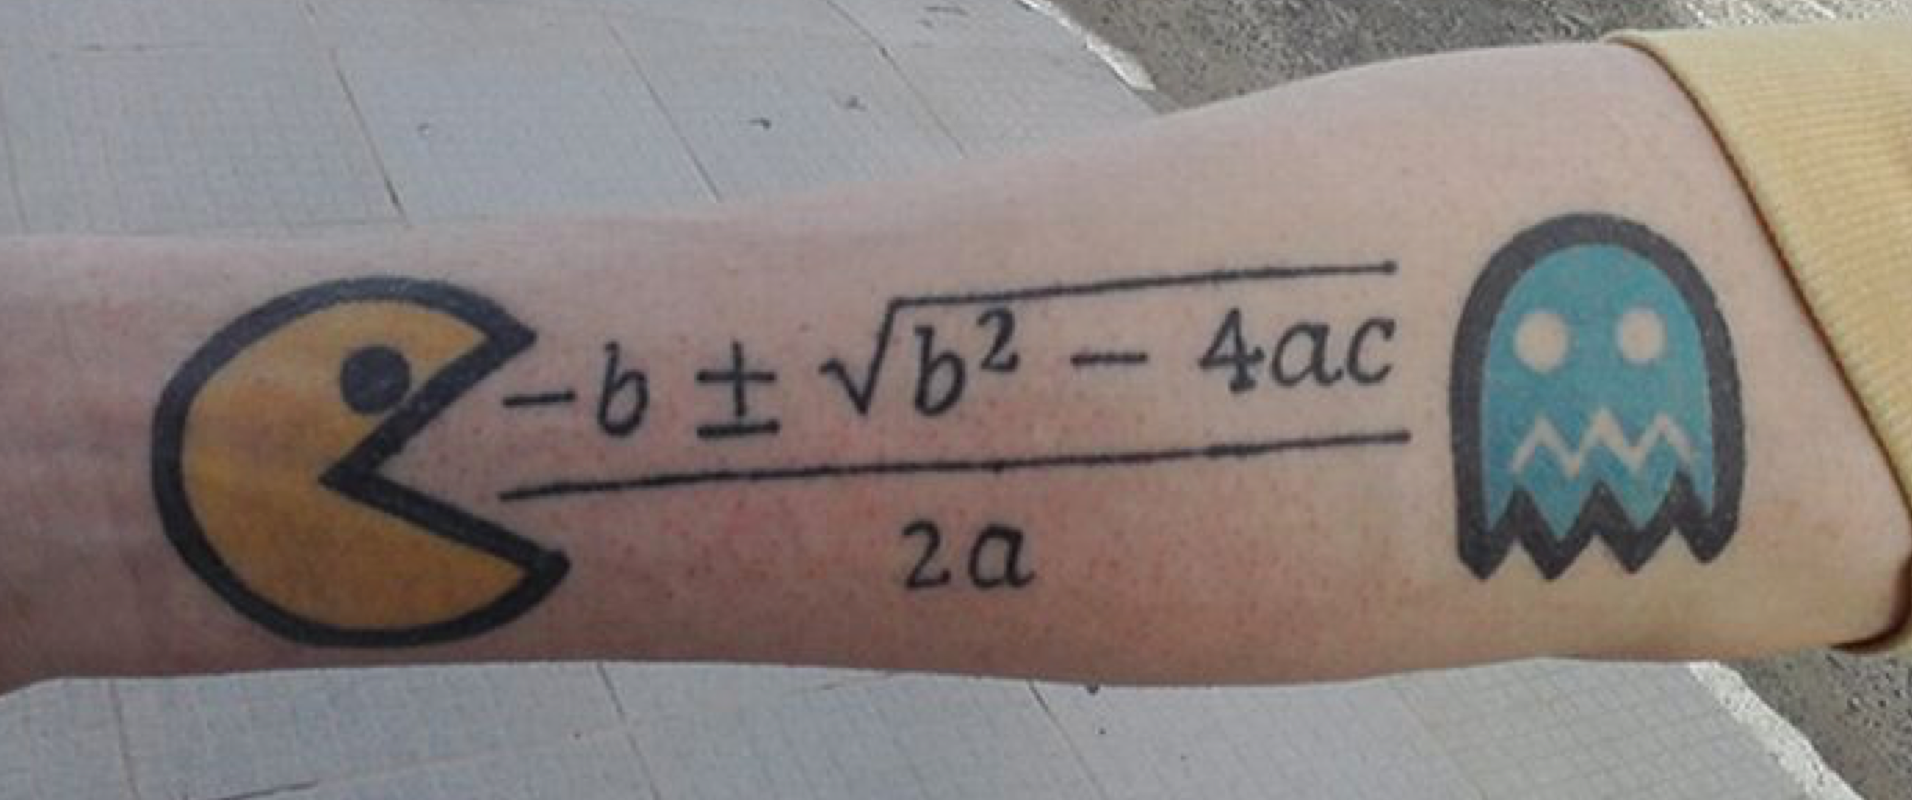
\includegraphics[width=.45\textwidth]{img-ecc/ecc07.png}
\end{figure}
\end{multicols}

\begin{miejemplo}
. Resuelve las ecuaciones: $\qquad  a)\ 6x^2+7x-20=0;\quad b)\ 2x^2+3x=0;\quad c)\ 4x^2-25$ 	

\vspace{5mm} $\triangleright \ \ a)\ \ 6x^2+7x-20=0 \to x=\dfrac{-7\pm \sqrt{7^2-4\cdot 6\cdot (-20)}}{2\cdot 6}=\dfrac{-7\pm \sqrt{49+480}}{12}=\dfrac{-7\pm 23}{12}\to \ x=4/3 \, \vee \, x=-5/2$

\vspace{5mm} $\triangleright \ \ b)\ \ 2x^2+3x=0 \ \ $ Es una ecuación de segundo grado incompleta en la que se puede sacar \emph{factor común} (se puede resolver por el método general con $a=2,\, b=3,\, c=0$):

$2x^2+3x=x\cdot(2x+3)=0 \to \begin{cases} \ \qquad \qquad x=0 & \text{una solución} \\ 2x+3=0 \to x=-3/2 & \text{otra solución} \end{cases}$


\vspace{5mm} $\triangleright \ \ c)\ \ 4x^2-25\ \ $  Es una ecuación de segundo grado incompleta en la que se puede \emph{despejar} (se puede resolver por el método general con $a=4,\, b=0,\, c=-25$):

$4x^2-25=0 \to 4x^2=25 \to x^2=\dfrac{25}{4} \ $ Sacando raíz cuadrada: $|x|=\dfrac 5 2 \to \begin{cases} \  x=\ \ 5/2  \\ \ x=-5/2\end{cases}$
\end{miejemplo}

\begin{miejercicio}

Resuelve las ecuaciones: $\qquad  a)\ x^2-2x+3=0;\qquad b)\ x^2-4x+4=0;\qquad c)\ 3x^2+27=0$

\rule{250pt}{0.1pt}

\vspace{2mm} $\triangleright \ \ a) \quad x=\dfrac{2\pm \sqrt{(-2)^2-4\cdot 1\cdot 3}}{2\cdot 1}=\dfrac{-2\pm \sqrt{-8}}{2} \ : \  \nexists \, \ $ No hay solución.

\vspace{5mm} $\triangleright \ \ b) \quad x=\dfrac{4\pm\sqrt{4^4-4\cdot 1 \cdot 4}}{2\cdot 1}=\dfrac{-4\pm 0}{2}=-2\ $ Solución doble.

\vspace{5mm} $\triangleright \ \ c)\ \quad  \text{ Incompleta (despejar) } \ 3x^2=-\ 27 \to x^2=-9 \to \ : \ \nexists \ $ No hay solución.	
\end{miejercicio}


\begin{theorem} [ Propiedades de las soluciones de la ecuación de segundo grado]

$\Box \ $ Sean $\ x_1=\dfrac{-b+\sqrt{b^2-4ac}}{2a} \ $ y  $\ x_2=\dfrac{-b-\sqrt{b^2-4ac}}{2a}\ $	las dos soluciones (raíces) de una ecuación de segundo grado $\ ax^2+bx+c=0$

\vspace{2mm} --- Suma de raíces: $\qquad \boldsymbol{ S\ = \ x_1+x_2} \ =\dfrac{-b+\sqrt{b^2-4ac}}{2a}+\dfrac{-b-\sqrt{b^2-4ac}}{2a}=\dfrac
{ -b + \cancel{ \sqrt{b^2-4ac} }  -b- \cancel{ \sqrt{b^2-4ac} } }
{2a}=\dfrac{-2b}{2a}= \ \boldsymbol{ -\dfrac b a}$

\vspace{2mm} --- Producto de raíces: $\qquad \boldsymbol{P\ = \ x_1\cdot x_2}\ = \dfrac{-b+\sqrt{b^2-4ac}}{2a} \cdot \dfrac{-b-\sqrt{b^2-4ac}}{2a} =
\vspace{2mm} \dfrac{-\cancel{b^2}- (\cancel{b^2}-4ac)}{4a^2}= \dfrac{4ac}{4a^2}= \ \boldsymbol{\dfrac c a}$

\vspace{2mm} $ax^2+bc+c=0 \ \to \ x^2+\dfrac b a x+\dfrac c a =0 \ \to \ x^2- \left( - \dfrac b a \right) x + \dfrac c a = 0 \, , \ $
por lo que son equivalentes las expresiones: $\quad  \boxed{ \ \boldsymbol{ ax^2+bx+c=0 \ \leftrightarrow \ a(x^2-Sx+P=0) } \ }\, $, con $S=x_1+x_2$ y $P=x_1\cdot x_2$

\vspace{7mm} $\Box \quad a(x-x_1)(x-x_2)=a(x^2-2(x_1+x_2)+x_1x_2)=a\left( x^2-\left( -\dfrac b a \right) x-\dfrac c a \right) = ax^2+bx+c $ 

\vspace{2mm} Luego, todo trinomio de segundo grado $ax^2+bx+c$ con raíces $x_1,\ x_2$ se puede factorizar como $ \quad \subrayado{ \boxed{ \  \boldsymbol{ax^2+bx+c \ = \ a(x-x_1)(x-x_2)} \ }}$
\end{theorem}


\subsection{Ecuaciones reducibles a segundo grado}
\begin{tikzpicture}
	\fill [left color=red!50, right color=teal!50] (0,0) rectangle (3.5,.01);
	\fill [left color=teal!50, right color=blue!50] (3.5,0) rectangle (7.5,.01);
	\end{tikzpicture}
\vspace{0.5cm}

\begin{definition}[ Ecuaciones reducibles a segundo grado (bicuadradas)]

Son ecuaciones del tipo: $\quad \boldsymbol{ax^{2n}+bx^n+c=0}\, . \ $  El  cambio $\ \boxed{\ \boldsymbol{x^n=t} \ } \ $ convierte la ecuación en una de segundo grado: $\ at^2+bt+c=0\, . \ $ 

\vspace{2mm} Una vez resuelta esta ecuación hay que deshacer el cambio establecido: $\ x=\sqrt[n]{t}$
	
\end{definition}


\begin{miejemplo}

Resuelve $\quad a)\ \ x^6-7x^3-8=0;\qquad b)\ \ x^4-3x^2-4=0;\qquad c) \ \ x^8+17x^4+16=0$	

\vspace{5mm} $\triangleright \quad a)\ \ x^3=t \ \to \ t^2-7t-8=0 \ \to \cdots \to \ \begin{cases}
	\ t=\ \ 8=x^3 & \to \ x=2 \\ \ t=-1=x^3 & \to \ x=-1 \end{cases}$

\vspace{5mm} $\triangleright \quad b)\ \ x^2=t \ \to \ t^2-3t-4=0 \ \to \cdots \to \ \begin{cases}
 \ t=\ \ 4=x^2 	 & \to \ x=2 \, \vee \, x=-2 \\ t=-1=x^2 & \to \ \nexists x
 \end{cases}$

\vspace{5mm} $\triangleright \quad c)\ \ x^4=t \ \to \ t^2+17t+16 = 0 \ \to \cdots \to \ \begin{cases} \ t=\ -1=x^4 & \to \ \nexists x \\ \ t=-16= x^4 &\to \ \nexists x \end{cases}$
\end{miejemplo}

\begin{miejercicio}

Resuelve: $\qquad a)\ \ x^4-4x^2=0;\qquad b)\ \ x^{12}+x^6=0; \qquad c) \ \ x^4-25x^2+144=0$	

\rule{250pt}{0.1pt}

\vspace{2mm} $\triangleright \ \ a)\ \ $ Incompleta, factor común: $\ x^2(x^2-4)=0 \to \begin{cases} \ x^2=0 & \to \ x=0 \\ \ x^2-4=0 & \to \ x=2\, \vee \ x=-2 \end{cases}$

\vspace{2mm} También se hubiera podido resolver con el cambio $\ x^2=t$

\vspace{5mm} $\triangleright \ \ b)\ \ $ Incompleta, factor común: $\ x^6(x^6+1)=0 \to \begin{cases} \ x^6=0 & \to \ x=0  \\ \ x^6+1=0 & \to x=\sqrt[6]{-1}\, \nexists \end{cases}$

\vspace{2mm} También se hubiera podido resolver con el cambio $\ x^6=t$

\vspace{5mm} $\triangleright \ \ c)\ \ x^2=t \to t^2-25t+144 = 0 \to \begin{cases} \ t=\ 4=x^2 & \to \ x=2 \, \vee \, x=-2 \\ t=16=x^2 & \to x=4 \, \vee \, x=-4  \end{cases}$
\end{miejercicio}

\vspace{5mm}

Las ecuaciones reducibles a segundo grado de la forma $ax^4+bx^2+c00$, que se resuelven con el cambio $x^2=t$, reciben el nombre de \textbf{bicuadradas}.



\vspace{0.5cm}
\subsection{Ecuaciones polinómicas}
\begin{tikzpicture}
	\fill [left color=red!50, right color=teal!50] (0,0) rectangle (3.5,.01);
	\fill [left color=teal!50, right color=blue!50] (3.5,0) rectangle (7.5,.01);
	\end{tikzpicture}
\vspace{0.5cm}


\begin{definition}[ Ecuación polinómica]

Una ecuación polinómica es la que está definida a partir de un polinomio.

$$a_0x^n+a_1x^{n-1}+\cdots +a_{n-2}x^2+a_{n-1}x+a_n=0$$	
\end{definition}


\begin{theorem}[ Resolución de ecuaciones polinómicas por factorización]
. Si la ecuación polinómica es de grado igual o superior al tercero y no es reducible a segundo grado, podemos \emph{factorizar} el polinomio y sus raíces serán las soluciones de la ecuación.

\vspace{2mm} Es importante advertir que de este modo solo encontraremos las raíces (soluciones) enteras si probamos por los divisores del término independiente o las soluciones racionales si probamos con divisores del término independiente divididas por divisores del término dominante. Nótese que todo lo dicho hasta el momento será cierto si el polinomio tiene todos sus coeficientes enteros.

\vspace{2mm} El teorema fundamental del álgebra asegura que una ecuación polinómica de grado $n$ tendrá, a lo sumo, $n$ raíces (incluyendo sus órdenes de multiplicidad).
\end{theorem}

\begin{myalertblock}{Imposibilidad de resolver por fórmulas generales las ecuaciones de cualquier grado mayor que 4}
	
	Después de los trabajos exitosos de Cardano, Tartaglia y Ferrari (soluciones a ecuaciones de tercer y cuarto grados), durante siglos muchos matemáticos buscaron de manera infructuosa una fórmula que diera las soluciones de cualquier ecuación de quinto grado. Fue Niels Henrik Abel (1802-1829) quien demostró de manera concluyente que tal fórmula general no existe. Por poco tiempo aún subsistió el problema de decidir para cuáles ecuaciones de grado 5 o superior sí existen tales fórmulas, pero este interrogante fue resuelto de manera final por Evariste Galois (1811-1832). Además de mostrar la \emph{imposibilidad de resolver por fórmulas generales las ecuaciones de cualquier grado mayor que 4}, sus trabajos dieron origen a la Teoría de Grupos.

\begin{flushright}
 Arnold Oostra. Revista Tumbaga (2008), 3, 174-186	
\end{flushright}
\end{myalertblock}


\vspace{5mm}

$a_0x^n+a_1x^{n-1}+\cdots +a_{n-2}x^2+a_{n-1}x+a_0= a_0(x-x_1)^{m_1}\cdot (x-x_2)^{m_2}\cdot \cdots \cdot (x-x_k)^{m_k} = 0 \ \to \ $

Raíces (soluciones) $\qquad \to \ \begin{cases}
\ x-x_1=0 &\to x=x_1 \ \text{ orden m}_1 \\
\ x-x_2=0 &\to x=x_2 \ \text{ orden m}_2 \\
\quad \cdots & \quad \quad \cdots \\
\ x-x_k=0 &\to x=x_k \ \text{ orden m}_k	
 \end{cases}$	


\vspace{2mm} \textcolor{gris}{Nos basamos en la propiedad de que el producto de dos números reales da cero si y solo si alguno de ellos es cero: 
$\quad a \cdot b = 0 \ \leftrightarrow \ a=0 \, \vee \, b=0 \, . \ $ Esto solo ocurre si el producto da cero, para cualquier otro número real hay infinitas posibilidades.}

\begin{miejemplo}

Resuelve: $\qquad x^{6} - 2 \; x^{5} - 18 \; x^{4} + 6 \; x^{3} + 41 \; x^{2} + 8 \; x + 60 = \ 0$	

\vspace{5mm} Ecuación polinómica de orden 6 no reducible a segundo grado $\to$ factorización por Ruffini. Posibles raíces $\pm\{1,2,3,45,6,10,12,15,20,30,60\}$

\begin{multicols}{2}
\begin{table}[H]
\centering
\begin{tabular}{r|rrrrrrr}
 & 1 & -2 & -18 & 6 & 41 & 8 & 60 \\
2 &  & 2 & 0 & -36 & -60 & -38 & -60 \\ \hline
 & 1 & 0 & -18 & -30 & -19 & \multicolumn{1}{r|}{-30} & 0 \\ \cline{8-8} 
-2 &  & -2 & 4 & 28 & 4 & 30 &  \\ \cline{1-7}
 & 1 & -2 & -14 & -2 & \multicolumn{1}{r|}{-15} & 0 &  \\ \cline{7-7}
-3 &  & -3 & 15 & -3 & 15 &  &  \\ \cline{1-6}
 & 1 & -5 & 1 & \multicolumn{1}{r|}{-5} & 0 &  &  \\ \cline{6-6}
5 &  & 5 & 0 & 5 &  &  &  \\ \cline{1-5}
 & 1 & 0 & \multicolumn{1}{r|}{1} & 0 &  &  &  \\ \cline{5-5}
\end{tabular}
\end{table}	

$(x-2)(x+2)(x+3)(x-5)(x^2+1)=0 \leftrightarrow $

%\vspace{2mm} 

$$\begin{cases}
 \ x-2=0 &\to \ x=2 \\	
 \ x+2=0 &\to \ x=-2 \\
 \ x+3=0 &\to \ x=-3 \\
 \ x-5=0 &\to \ x=5 \\
 \ x^2+1=0 &\to \ \nexists x
 \end{cases}$$

\end{multicols}

\end{miejemplo}



\begin{miejercicio}

Resuelve: $\qquad a)\ \ 6x^5+7x^4-9x^3+2x^2=0;\qquad \qquad b)\ \ x^6+x^5-8x^4-8x^3+16x^2+16x=0$

\rule{250pt}{0.1pt}

\vspace{2mm} $\triangleright \quad a) \quad $ Primero, al carecer de término independiente, sacamos factor común. Ahora, el término independiente es $16$ y las posibles raíces $\pm\{1,2,4,8,16\}$. Factorizando el polinomio por Ruffini, como aprendimos el tema anterior:

\vspace{2mm} $6x^5+7x^4-9x^3+2x^2=x^2(x+2)(6x^2+5x+1)=0 \to $

\vspace{2mm} $\qquad \qquad  \to \begin{cases}
 	\ x^2=0  \to \ x=0,\ \text{doble} \\ \ x=-2 \\ 6x^2+5x+1=0 \to \begin{cases}
 	\ x=1/2 \\ \ x=1/3 
 	\end{cases}
 \end{cases}$


\vspace{5mm} $\triangleright \quad b) \quad $ Del mismo modo:

\vspace{2mm} $x^6+x^5-8x^4-8x^3+16x^2+16x=x(x+1)(x-2)^2(x+2)^2=0 \to $

\vspace{2mm} $\qquad \qquad \to \begin{cases}
 	\ x=0 \\ \ (x+1)=0 \to \ x=-1 \\ \ (x-2)^2= 0 \to (x-2)= 0 & \to x=2,\ \text{doble} \\ \ (x+2)^2= 0 \to (x+2)= 0 & \to  x=-2,\ \text{doble}
 \end{cases}$
\end{miejercicio}


\vspace{10mm}
\begin{figure}[H]
	\centering
	
\includegraphics[width=.95\textwidth]{img-ecc/ecc08.png}
\end{figure}

\vspace{1cm}
\section{Ecuaciones racionales}
\begin{tikzpicture}
	\fill [left color=red!50, right color=teal!50] (0,0) rectangle (3.5,.1);
	\fill [left color=teal!50, right color=blue!50] (3.5,0) rectangle (7.5,.1);
	\end{tikzpicture}
\vspace{0.5cm}


\begin{definition}[ Ecuación racional]

Son ecuaciones sobre fracciones algebraicas: $\qquad \dfrac{p(x)}{q(x)}+	\dfrac{r(x)}{s(x)}+\cdots = 0$
\end{definition}



\begin{theorem}[ Resolución de ecuaciones racionales]

Para resolverlas se multiplicará toda la ecuación por el MCM de los denominadores, por lo que tal vez haya que realizar antes algunas operaciones (paréntesis). Con este procedimiento la ecuación racional se convertirá en una ecuación polinómica.


\vspace{5mm} 
\begin{destacado}
\begin{small}
 \textcolor{red}{$\boldsymbol{\boxed{ \ ! \ }} $}  $\ $ \textbf{Resuelta la ecuación hay que comprobar que \emph{las soluciones obtenidas no anulan ningún denominador en la ecuación de partida}.}
 \end{small}
 \end{destacado}
	
\end{theorem}

\begin{miejemplo}

Resuelve: $ \quad \dfrac{x+1}{x-1}-1=\dfrac 1 x$

\vspace{5mm} $MCM:\ \ x(x-1) \ \to \ 	x \cancel{(x-1)} \cdot \dfrac{x+1}{\cancel{(x-1)}}-x(x-1) \cdot 1=\cancel{x} (x-1) \cdot \dfrac 1 {\cancel{x}}$

$x(x+1)=x(x-1)=x-1 \ \to \ x=-1 \ $ Solución (única) que no anula ningún denominador en la ecuación de partida.
\end{miejemplo}

\begin{miejercicio}

Resuelve: $\qquad a)\ \ \dfrac{x+1}{3x-6}-\dfrac{x-1}{2x+4}=\dfrac{10-x^2}{6x^2-24};\qquad b)\ \ 	\dfrac{x}{x+1}-\dfrac{1}{x}=\dfrac{3x+2}{x+1}$

\rule{250pt}{0.1pt}

\vspace{2mm} $\triangleright \quad a)\  $ denominadores:
$3\ x-6=3(x-2);\ \ 2x+4=2(x+2);\ \ 6x^2-24=6(x+2)(x-2) \ \ \to \ \ MCM=6(x+2)(x-2)$

\vspace{2mm} $6(x+2)(x-2) \cdot \dfrac{x+1}{3(x-2)}-6(x+2)(x-2) \cdot \dfrac{x-1}{2(x+2)}=6(x+2)(x-2) \cdot \dfrac{10-x^2}{6(x+2)(x-2)} \to 2(x-2)(x+1)-3(x-2)(x-1)=10-x^2 \ \to \ 15x-12=0 \ \to x=4/5 \ $ Solución (única) que no anula ningún denominador en la ecuación de partida.

\vspace{5mm} $\triangleright \quad b)\ $ Denominadores: $\ MCM=x(x+1)$

\vspace{2mm} $x(x+1)\cdot \dfrac{x}{x+1}-x(x+1)\cdot \dfrac{1}{x}=x(x+1)\cdot \dfrac{3x+2}{x+1} \to \ 2x^2+3x+1=0 \to $

\vspace{2mm} $\to \begin{cases}
 	\ x=-1/2 & \text{ Solución buena, no anula ningún denominador de partida} \\ \ \cancel{\bcancel{ \boldsymbol{ x=-1 }}} & \text{ Solución mala, anula denominadores en la ecc. de partida}
 \end{cases}$

\vspace{2mm} La única solución de esta ecuación es $\ x=-1/2$

\end{miejercicio}


\vspace{1cm}
\section{Ecuaciones irracionales}
\begin{tikzpicture}
	\fill [left color=red!50, right color=teal!50] (0,0) rectangle (3.5,.1);
	\fill [left color=teal!50, right color=blue!50] (3.5,0) rectangle (7.5,.1);
	\end{tikzpicture}
\vspace{0.5cm}


%%%%%%%%%%%%%%%%%%%%%%%%%%
\begin{definition}[ Ecuaciones con raíces cuadradas]

Una ecuación con raíces cuadradas, también llamada ecuación irracional, es aquella en las que la incógnita  aparece bajo el signo de la radical.
\end{definition}

\begin{theorem}[ Resolución de ecuaciones con radicales]


\begin{enumerate}

\item Se aísla el radical en un miembro de la igualdad pasando los restantes términos al otro miembro.


\item Se elevan al cuadrado los dos miembros de la ecuación, con lo que desaparecerá la raíz.


\item Si todavía queda algún radical, se repite el proceso anterior.


\item Se resuelve la ecuación resultante y se \underline{comprueba siempre}$^{(*)}$ cuáles de las soluciones obtenidas verifican la ecuación con radicales de partida.
\end{enumerate}

\vspace{5mm} 
\begin{destacado}
\begin{small}
 \textcolor{red}{$\boldsymbol{\boxed{ \ ! \ }} $}  $\ $ \textbf{Resuelta la ecuación irracional hay que comprobar que \emph{las soluciones obtenidas cumplen la ecuación de partida}.}
 \end{small}
 \end{destacado}

\end{theorem}

$^{(*)}$  Es necesaria siempre la comprobación de las soluciones que se obtengan al resolver este tipo de ecuaciones porque al elevar al cuadrado se pueden introducir soluciones no deseables. P.e.: $\quad x=2 \to x^2=2^2=4 \to \sqrt{x^2}=|x|=2 \ \to x=2 \text{ buena solución; } \cancel{\bcancel{x=-2}} \text{ solución mala}$

\begin{miejemplo}

Resuelve: $\quad x+3\sqrt{x+1}=17$

\vspace{5mm} Paso 1: $\quad x+3\sqrt{x+1}=17 \ \to \ 3\sqrt{x+1}=17-x$

\vspace{2mm} Paso 2: $\quad \left( 3\sqrt{x+1}\right)^2=(17-x)^2 \to 9(x+1)=289-34x+x^2$

\vspace{2mm} No quedan más raíces. No se hace el Paso 3. Resolvemos ahora nuestra ecuación:

\vspace{2mm} Paso 4:  $\quad x^2-43x+280=0 \to \begin{cases} \ x=8 \\ \ x=35 \end{cases}$

\vspace{2mm} Hay que \underline{comprobar} cada una de las soluciones obtenidas en la ecuación de partida. 

\vspace{2mm} $x=8 \to  8+3\sqrt{8+1} = 8+3\cdot 3 = 17 \to \boldsymbol{x=8}\ $ Buena solución.

\vspace{2mm} $x=35 \to  35+3\sqrt{35+1}=35+3\cdot 6=35+18  \ \boldsymbol{\neq} \  17 \to $ Mala solución.

\vspace{2mm} La única solución a nuestra ecuación es: $\quad x=8$.
	
\end{miejemplo}


\begin{miejercicio}

Resuelve las ecuaciones: 

\begin{multicols}{2}
\begin{enumerate}[a) ]
\item $\sqrt{5x+6}=3+2x$
\item $x+\sqrt{7-3x}=1$
\item $\sqrt{3x+4}-\sqrt{1-x}=1$
\item $\sqrt{2x+3}+\sqrt{x-5}=0$	
\end{enumerate}
\end{multicols}

\rule{250pt}{0.1pt}

\vspace{2mm} $\triangleright \ \ a)\ \ \sqrt{5x+6}=3+2x \to \ (\sqrt{5x+6})^2=(3+2x)^2 \to 5x+6=9+12x+4x^2  $

\vspace{2mm} $4x^2+7x+3=0 \to \begin{cases} \ x=-1 \\ \ x=-3/4 \end{cases} \ $ Ahora debemos comprobar los resultados.


\vspace{2mm} $x=-1 \to \sqrt{5(-1)+6} \ ? \  3+2(-1);\ \ 1=3-2 \ $ Sí. Sol. buena.

\vspace{2mm} $x=-3/4 \to \sqrt{5(-3/4)+6}\ ? \ 3+2(-3/4);\ \  \sqrt{-\frac {15}{4} +6} \ ? \ 3-\frac 3 2;\ \ \sqrt{9 4}=\frac 3 2 $ Sí. Sol. buena.

\vspace{2mm} La ecuación tiene dos soluciones válidas, $\ x=-1 \ \wedge \ x=-3/4$

\vspace{5mm} $\triangleright \ \ b)\ \ x+\sqrt{7-3x}=1 \to (\sqrt{7-3x})^2=(1-x)^2 \to 7-3x=1-2x+x^2$

\vspace{2mm} $x^2+x-6=0 \to \begin{cases}\ x=2 \\ \ x=-3 \end{cases}\ $ Ahora debemos comprobar los resultados.

\vspace{2mm} $x=2 \to 2+\sqrt{7-3\cdot 2} \ ? \ 1 \to 2+1 \neq 1 \to $ No. Sol. mala.

\vspace{2mm} $x=-3 \to -3+\sqrt{7-3(-3)}\ ? \ 1 \to -3+4=1\ $ Sí. Sol. buena.

\vspace{2mm} La única solución de la ecuación es $\ x=-3$


\vspace{5mm} $\triangleright \ \ c)\ \ \sqrt{3x+4}-\sqrt{1-x}=1$

\vspace{2mm} Tenemos dos raíces cuadradas. No podemos dejar una sola raíz en un término de la ecuación, al elevar al cuadrado aparecerá una nueva raíz.

\vspace{2mm} $(*) \quad (\sqrt{3x+4}-\sqrt{1-x})^2=1^2 \to (3x+4) -2 \sqrt{3x+4}\cdot \sqrt{1-x} + (1-x)=1$ 

\vspace{2mm} Aislamos la nueva raíz $\ 2x+4=2\sqrt{(3x+4)(1-x)}\ $ y elevamos al cuadrado.

\vspace{2mm} $ (2x+4)^2=(2\sqrt{(3x+4)(1-x)})\  \to  \ 4x^2+16x+16=4\,(3x+4)(1-x)$

\vspace{2mm} $4x^2+16x+16=-12x^2-4x+16 \ \to \ 16x^2+20x=0=x(16x+20) \to  \begin{cases} \ x=0 \\ x=-5/4 \end{cases}$

\vspace{2mm} Hubiese sido mejor dejar una raíz en cada miembro de la ecuación, la raíz que no quede aislada, al elevar al cuadrado volverá a producir una raíz pero más sencilla que anteriormente.

\vspace{2mm} $(**) \quad (\sqrt{3x+4}=(1+\sqrt{1-x})^2\ \to \ (3x+4)=1+2\sqrt{1-x}+(1-x) \ \to \ 4x+2=2\sqrt{1-x}$

\vspace{2mm} $(4x+2)^2=(2\sqrt{1-x})^2 \ \to \ 16x^2+16x+4=4(1-x)  \to \ 16x^2+20x=0=x(16x+20) \to  $

\vspace{2mm} $\to \begin{cases} \ x=0 \\ x=-5/4 \end{cases}\ $ Son más sencillos los cálculos en este caso (una raíz en cada miembro, una de ellas aislada). Por $(*) \  \text{ o por } (**) \ $ tenemos, del mismo modo, que  $x=0\ \wedge \ x=-5/4$. Hay que comprobar las soluciones.

\vspace{2mm} $x=0 \to \sqrt{3\cdot 0+4}-\sqrt{1-0}\ ? \ 1 \to 2-1=1\ $ Sí. Buena solución.

\vspace{2mm} $x=-5/4 \ \to \ \sqrt{3(-5/4)+4}-\sqrt{1-(-5/4)} \ ? \ 1 \ \to \ \sqrt{-\frac {15}{4}+1}-\sqrt{1+\frac 5 4}\ ? \ 1 \ \to \ \sqrt{\frac 1 4}-\sqrt{\frac 9 4 } \ ? \ 1 \ \to \ \frac 1 2 - \frac 3 2 \neq 1 \ $ No. Mala solución.

\vspace{2mm} \normalsize{La} ecuación tiene una sola solución, $x=0$.

\vspace{5mm} $\triangleright \ \ d)\ \ \sqrt{2x+3}+\sqrt{x-5}=0$
	
\vspace{2mm} En esta ocasión, al ser cero el segundo término, es mucho más sencillo aún disponer una raíz en cada término. Sl elevar al cuadrado ambos términos desaparecerán ambas raíces.

\vspace{2mm} $\sqrt{2x+3}+\sqrt{x-5}=0 \to \ (\sqrt{2x+3})^2=(-\sqrt{x-5})^2 \to 2x+3=x-5 \to x=-8$

\vspace{2mm} Hay que comprobar la solución: $\ \ \sqrt{2(-8)+3}+\sqrt{(-8)-5}=0 \to \nexists \sqrt{-13} \ $ por lo que la solución No es válida. Solución mala.

\vspace{2mm} Esta ecuación no tiene soluciones.
	
\end{miejercicio}


\vspace{1cm}
\section{Ecuaciones exponenciales}
\begin{tikzpicture}
	\fill [left color=red!50, right color=teal!50] (0,0) rectangle (3.5,.1);
	\fill [left color=teal!50, right color=blue!50] (3.5,0) rectangle (7.5,.1);
	\end{tikzpicture}
\vspace{0.5cm}


\begin{definition}[ Ecuación exponencial]
. Una ecuación exponencial es aquella en la que la incógnita aparece en el exponente.

$$a^x>0,\ \forall x \in \mathbb R;\qquad x^a=x^b \Rightarrow a=b,\	 \forall a,b \in \mathbb R,\ x\in \mathbb R^+ \smallsetminus \{1\}$$
\end{definition}

\begin{theorem}[ Resolución ecuaciones exponenciales]
. Resolveremos ecuaciones exponenciales: 
\begin{itemize}
\item Expresando, si es posible, ambos miembros de la ecuación como potencias de la misma base e igualando los exponentes.
\item Tomando logaritmos en ambos miembros de la ecuación.
\item Efectuando un cambio de variable $(a^x=t)$. Al final hay que recordar deshacer el cambio de variable establecido.	
\end{itemize}
\end{theorem}

\begin{miejemplo}

$\triangleright \quad \boldsymbol{3^{x-1}=\dfrac 1{27}} \ \to \ 3^{x-1}=\dfrac 1{3^3}\ \to \ 3^{x-1}=3^{-3}\ \Rightarrow \ x-1=-3 \ \to \ \boldsymbol{x=-2}$

\vspace{2mm} Ambos miembros se pueden escribir como una potencia de 3.

\vspace{4mm} $\triangleright \quad \boldsymbol{3^{x-1}=8} \ \Rightarrow \ \ln 3^{x-1}=\ln 8 \ \to \ (x-1)\ln 3= \ln 8 \ \to \ x-1=\dfrac{ln8}{ln3} \ \to \  \boldsymbol{x=1+\dfrac{ln8}{ln3}}$

\vspace{2mm} Un miembro es una potencia de 3 y el otro no. Tomamos logaritmos naturales a ambos lados de la ecuación.

\vspace{4mm} $\triangleright \quad \boldsymbol{3^{x-1}+3^x=4} \ \Rightarrow \ \text{Cambio de variable: } \ \boldsymbol{3^x=t};\ \ 3^{x-1}=\dfrac{3^x}{3}=\dfrac t 3 \ \ \to \ \dfrac t 3 + t=4 \ \to $

$\to \ 4t=12 \ \to \  t=3=3^x \ \Rightarrow \ 3^x=3 \textcolor{gris}{=3^1} \ \to \ \boldsymbol{x=1}$

\vspace{2mm} Aparecen sumas de potencias en un miembro.	Hacemos un cambio de variables, que luego hay que deshacer.
\end{miejemplo}

\begin{miejercicio}

Resuelve: 
\begin{multicols}{2}
  \begin{enumerate}[a) ]
	\item $7^{x-1}=2^{x+5}$

	\item $3^{x-1}+3^x+3^{x+1}=117$

	\item $5^{2x}-30\cdot 5^x+125=0$ 	

	\item $3\cdot 4^{x+1}+2\cdot 2^{x+3}=11$
  \end{enumerate}
\end{multicols}

\rule{250pt}{0.1pt}

\vspace{2mm} $\triangleright \ \ a)\quad 7^{x-1}=2^{x+5}$

\vspace{2mm} Tenemos dos potencias igualadas de distinta base, tomaremos logaritmos (decimales, en este caso, para variar.)

\vspace{2mm} $\mathrm{Log} \, 7^{x-1}=\mathrm{Log} \, 2^{x+5} \ \to \ (x-1) \mathrm{Log} \, 7 = (x+5) \mathrm{Log} \, 2 \ \to \ $

\vspace{2mm}$\to \ x\mathrm{Log}\, 7 -x\mathrm{Log}\, 2=5\mathrm{Log} \, 2+\mathrm{Log}\,7 \to  x(\mathrm{Log}\, 7 -\mathrm{Log}\, 2)=5\mathrm{Log} \, 2+\mathrm{Log}\,7 \ \to \ $
 
\vspace{2mm} $\to \ \boldsymbol{x=\dfrac{5\mathrm{Log} \, 2+\mathrm{Log}\,7}{\mathrm{Log}\, 7 -\mathrm{Log}\, 2}}$



\vspace{5mm} $\triangleright \ \ b)\quad 3^{x-1}+3^x+3^{x+1}=117$

\vspace{2mm} Aparecen sumas de varias potencias, estableceremos un cambio de base: llamamos $\boldsymbol{3^x=t}$, por lo que $3^{x-1}=\frac {3^x}3=\frac t 3;\ 3^{x+1}=3^x\cdot 3=3t$

\vspace{2mm} $\dfrac t 3 +t+3t=117 \ \to \ t+3t+9t=3\cdot 117 \ \to 13t=351 \ \to \ t=\dfrac{351}{13}=27\ = 3^x$

\vspace{2mm} Ahora hay que deshacer el cambio de variable: $3^x=27=3^3 \ \to \ \boldsymbol{x=3}$

\vspace{5mm} $\triangleright \ \ c)\quad 5^{2x}-30\cdot 5^x+125=0$

\vspace{2mm} Aparecen sumas de varias potencias, estableceremos un cambio de base: llamamos  $\boldsymbol{5^x=t}\ \to \ 5^{2x}=(5^x)^2=t^2$

\vspace{2mm} $t^2-30t+125=0 \to \text{ (ec. 2o grado) }\begin{cases}  \ t=25 \\ \ t=5 \end{cases}$

\vspace{2mm} Ahora deshacemos en cambio de variable: $\ \ \begin{cases} \ t=25=5^x & \to \boldsymbol{x=2} \\ \ t=5 =5^x &\to \boldsymbol{x=1} \end{cases}$ 

\vspace{5mm} $\triangleright \ \ d)\quad 3\cdot 4^{x+1}+2\cdot 2^{x+3}=11$

\vspace{2mm} Aparecen sumas de varias potencias, estableceremos un cambio de base: llamamos $\boldsymbol{2^x=t}$, entonces, $\begin{cases} \ 2^{x+3}=2^x\cdot 2^3=8t \\ \ 4^{x+1}=4^x\cdot 4=4\cdot(2^2)^x=4\cdot (2^x)^2=4t^2 \end{cases}$, por lo que

\vspace{2mm} $3(4t^2)+2(8t)=11\ \to \ 12t^2+16t-11=0 \to \text{ (ec. 2o grado) }\begin{cases}  \ t=1/2 \\ \ t=-11/6 \end{cases}$


\vspace{2mm} Ahora, deshacer el cambio de variable: $\begin{cases}
\ t=\dfrac 1 2 = 2^{-1}=2^x	 &\to \boldsymbol{x=-1} \\
\ t=-\dfrac{11}{6}=2^x &\to \boldsymbol{\nexists x }, \ (2^x>0,\ \forall x)
\end{cases}$
\end{miejercicio}



\vspace{1cm}
\section{Ecuaciones logarítmicas}
\begin{tikzpicture}
	\fill [left color=red!50, right color=teal!50] (0,0) rectangle (3.5,.1);
	\fill [left color=teal!50, right color=blue!50] (3.5,0) rectangle (7.5,.1);
	\end{tikzpicture}
\vspace{0.5cm}

\begin{definition}[ Ecuación logarítmica]

Una ecuación logarítmica es aquella en la que la incógnita aparece como argumento de un logaritmo.

$$\log_a(A)=\log_a(B) \ \ \Rightarrow \ \ A=B$$
\end{definition}

\begin{theorem}[ Resolución de ecuaciones logarítmicas]
. Usaremos las propiedades de los logaritmos.	

\vspace{5mm} 
\begin{destacado}
\begin{small}
 \textcolor{red}{$\boldsymbol{\boxed{ \ ! \ }} $}  $\ $ \textbf{Resuelta la ecuación logarítmica hay que comprobar que \emph{las soluciones obtenidas proporcionan argumentos de los logaritmos \textbf{positivos} al sustituir en la ecuación inicial}.}
 \end{small}
 \end{destacado}
\end{theorem}


\begin{miejemplo}
	. Resuelve $\qquad \mathrm{log}\, (x-4)+\mathrm{log}\, (x+5)=1$
	
\vspace{5mm} $\mathrm{log}\, [\, (x-4)\cdot (x+5) \, ]=\mathrm{log}\, 10 \to (x-4)(x+5)=10 \to x^2+x-30=0$

\vspace{2mm} Ecuación segundo grado $\ \to \ x=5 \ \vee \ x=-6$ Hay que comprobar ambas soluciones, que no aparezca ningún argumento no positivo en los logaritmos de la ecuación inicia.

\vspace{2mm} $x=5 \to \begin{cases} x-4=5-4=1>0 \\ x+5=5+5=10>0 \end{cases} \ \boldsymbol{ x=5}\ $ solución buena.

\vspace{2mm} $x=-6 \to \begin{cases} x-4=-6-4=-10<0 \\ x+5=-6+5=-1<0 \end{cases} \ \cancel{\bcancel{\boldsymbol{x=5}}}\ $ solución mala.

\vspace{2mm} Esta ecuación solo tiene una solución, $\ \boldsymbol{x=5}$
\end{miejemplo}

\begin{miejercicio}

Resuelve las siguientes ecuaciones:

\begin{small}
\begin{multicols}{2}
\begin{enumerate}[a) ]
\item $\mathrm{log}\, (x^2-9)-\mathrm{log}\, (x-3)=\mathrm{log}\, 3+\mathrm{log}\, 2x$
\item $3\ln x=\ln 3x+\ln(2x-3)$ 	
\item $\ln 4-\ln(x+2)-\ln(3x-4)+\ln x=0$
\item $2\log_2 x^3=3+\log_2 x$
\item $\log_3 x=\log_9 4$
\item $\log_{x+3}9=\lg_5 3$
\end{enumerate}	
\end{multicols}
\end{small}

\rule{250pt}{0.1pt}

\vspace{5mm} $\triangleright \ \ a) \quad  \mathrm{log}\, (x^2-9)-\mathrm{log}\, (x-3)=\mathrm{log}\, 3+\mathrm{log}\, 2x$

\vspace{2mm} $\log \dfrac{x^2-9}{x-3}=\log 3\cdot 2x \ \to \  \dfrac{x^2-9}{x-3}= \dfrac{(x+3)\cancel{(x-3)}}{\cancel{(x-3)}}=x+3=6x \ \to $

\vspace{2mm} $\to \ 3=5x \ \to \ x=\dfrac 5 3 \ $ Solución buena pues no produce ningún argumento negativo o cero en los logaritmos de la ecuación de partida.


\vspace{5mm} $\triangleright \ \ b) \quad  3\ln x=\ln 3x+\ln(2x-3)$

\vspace{2mm} $\ln x^3=\ln 3x(2x-3) \ \to \ x^3=6x^2-9x \ \to \ x^3-6x^2+9x=0 \ \to \ x(x^2-6x+9)=0 \ \to$

\vspace{2mm} completando cuadrados, $\ \to \  x(x-3)^2=0 \ \to \ \begin{cases}
\ x=0 & \text{ Sol. mala, } \nexists \ln 0 \\
\ x= 3 & \text{ Sol.buena, no } \ln (\le 0)  	
 \end{cases}$

\vspace{5mm} $\triangleright \ \ c) \quad  \ln 4-\ln(x+2)-\ln(3x-4)+\ln x=0$

\vspace{2mm} $  \ln 4-\ln(x+2)=\ln(3x-4)-\ln x \ \to \ \ln \dfrac{4}{x+2}=\ln \dfrac {3x-4}{x}\ \to \ \dfrac{4}{x+2}=\dfrac{3x-4}{x}\ \to$

\vspace{2mm} $\to \ 4x=(x+2)(3x-4) \ \to \ 3x^2-2x-12=0 \ \to \ \begin{cases}
 \ x=2 &  \nexists \ln(\le 0) \text{ buena}  \\ \ x=-4/3 &	\exists \ln(\le 0) \text{ mala}
 \end{cases}$
 
 \vspace{2mm} La única solución de esta ecuación es $x=2$


\vspace{5mm} $\triangleright \ \ d) \quad  2\log_2 x^3=3+3\log_2 x$

\vspace{2mm} Como $3=3\cdot 1=3\, \lg_2 2=\log_2 2^3=\log_2 8$, podemos escribir

\vspace{2mm} $ 2\log_2 x^3=\log_2 8+\log_2 x^3 \ \to \ \log_2 (x^3)^2=\log_2 (8\cdot x^3) \ \to \ \log_2 x^6=\log_2 8x^3 \ \to $

\vspace{2mm}$\to \ x^6-8x^3=0 \ \to \ x^3(x^3-8)=0 \ \to  \ \begin{cases}
 \ x=2 &  \nexists \ln(\le 0) \text{ buena}  \\ 
 \ x=0 &	\exists \ln(\le 0) \text{ mala}	
 \end{cases}$

\vspace{2mm} La única solución de esta ecuación es $x=2$

\vspace{5mm} $\triangleright \ \ e) \quad  \log_3 x=\log_9 4$


\vspace{2mm} Usamos la fórmula del cambio de base de la función logarítmica y lo expresamos todo en función de $\log_3$, por ejemplo.

\vspace{2mm} $\log_3 x=\dfrac{\log_3 4}{\log_3 9}\, ; \ $ como $\log_39=\log_33^2=2\cancelto{1}{\log_3 3}=2\quad \to \quad \log_3 x=\dfrac{\log_3 4}{2} \ \to \ $

\vspace{2mm} $2\log_3 x=\log_3 4 \ \to \ \log_3 x^2=\log_3 4 \ \to \  \ \begin{cases}
 \ x=2 &  \nexists \ln(\le 0) \text{ buena}  \\ 
 \ x=-2 &	\exists \ln(\le 0) \text{ mala}	
 \end{cases}$

\vspace{2mm} La única solución de esta ecuación es $x=2$

\vspace{5mm} $\triangleright \ \ f) \quad  \log_{x+3}9=\lg_5 3$
	
\vspace{2mm} Usamos la fórmula del cambio de base de la función logarítmica y lo expresamos todo en función de $\log_3$

\vspace{2mm} $\dfrac{\log_3 9}{\log_3(x+3)}=\dfrac{\log_3 3}{\log_3 5}\quad  $ Como $log_3 3=1 \ $ y $ \ \log_3 9=\log_3 3^2=2\log_3 3=2\, , \ $

\vspace{2mm} $ \dfrac{2}{\log_3(x+3)}=\dfrac{1}{\log_3 5} \ \to \ \log_3(x+3)=2\log_3 5=\log_3 5^2=\log_3 25 \ \to $

\vspace{2mm} $\to x+3=25 \ \to \ x=22$, solución buena al no hacer que $\nexists \ln(\le 0)$ en ecuación inicial.


\end{miejercicio}

\vspace{1cm}
\section{Ecuaciones con valor absoluto}
\begin{tikzpicture}
	\fill [left color=red!50, right color=teal!50] (0,0) rectangle (3.5,.1);
	\fill [left color=teal!50, right color=blue!50] (3.5,0) rectangle (7.5,.1);
	\end{tikzpicture}
\vspace{0.5cm}

\begin{definition}[ Ecuaciones con valor absoluto]

\begin{theorem}[ Resolución]
. El conjunto de soluciones de una ecuación con valor absoluto viene dado por la siguiente relación:
$\quad |x| = a      \leftrightarrow       x = a    \ \vee \     x = - a\, , \  $
dados $x , a \in \mathbb R  \ \wedge \   a > 0 $
\end{theorem}

\vspace{5mm} 
\begin{destacado}
\begin{small}
 \textcolor{red}{$\boldsymbol{\boxed{ \ ! \ }} $}  $\ $ \textbf{En ecuaciones complicadas (aparece x dentro y fuera del valor absoluto) hay que comprobar \emph{las soluciones obtenidas cumplen la ecuación de partida}. Si estas ecuaciones se resuelven con rigor, estudiando los signos y las zonas de validez, no será necesario.}
 \end{small}
 \end{destacado}
\end{definition}

\begin{miejemplo}
	
	$\left| \dfrac{x+1}{x-5} \right| = 1 \ (\ge 0) \quad \begin{cases}
 \ \dfrac{x+1}{x-5}=1  \ \to \ x+1=x-5 \ \to \ 1=-5 \text{ No puede ser, }  \nexists \text{sol} \\ \\
 \ \dfrac{x+1}{x-5}=-1  \ \to \ x+1=-x+5 \ \to \ 2x=4 \ \to \ x=2 \text{ sol}	
 \end{cases}$
 
\vspace{2mm}  Esta ecuación solo tiene una solución, $\ x=2$
\end{miejemplo}

\begin{miejercicio}

Resuelve la ecuación: $\quad |x+6|=2x+6$

\rule{250pt}{0.1pt}

\vspace{2mm} Primer método, requiere comprobación:

\vspace{2mm} $|x+6|=2x+6 \ \to \ \begin{cases}
\ x+6= \ \ 2x+6 \ \to \ x=0 \\
\ x+6=-(2x+6) \to 3x=-12 \to x=-4	
\end{cases}$


\vspace{2mm} Comprobación: 

\vspace{2mm} $x=0 \ \to |0+6|=|6|=6; \ 2\cdot 0+6=0+6=6\; \ 6=6 \to \text{ Buena (solución válida)}$

\vspace{2mm} $x=-4 \ \to |-4+6|=|2|=2; \ 2\cdot (-4)+6=-8+6=6-2; \ 2\neq -2 \to \text{ Mala (solución no válida)}$

\vspace{2mm} La única solución de esta ecuación es $\ x=0$

\vspace{5mm} Segundo método, con rigor matemático. No hará falta comprobación posterior.

\vspace{2mm} $x+6=0 \leftrightarrow x=-6\ $ Distinguiremos cuando $\ x<6\ $ (que $|x+6|=-(x+6)) \ $ y cuando $\ x\ge 6\ $ (que $|x+16|=x+6$)

% Please add the following required packages to your document preamble:
% \usepackage{multirow}
\begin{table}[H]
\centering
\begin{tabular}{l|c|c|}
\cline{2-3}
 & $]-\infty,-6[$ & $]-6,+\infty[$ \\ \hline
\multicolumn{1}{|l|}{$|x+6|$} & $-x-6$ & $x+6$ \\ \hline
\multicolumn{1}{|l|}{\multirow{4}{*}{$|x+6|=2x+6\quad$}} & $-x-6=2x+6$ & $x+6=2x+6$ \\
\multicolumn{1}{|l|}{} & $3x=12$ & $3x=0$ \\
\multicolumn{1}{|l|}{} & $x=4$ & $\boldsymbol{x=0}$ \\
\multicolumn{1}{|l|}{} & $4 \notin ]-\infty,-6[$ & $0\in [-6,\infty[$ \\ \hline
\end{tabular}
\end{table}

Solución, $\ x=0$	
\end{miejercicio}


\begin{miejercicio}

Resuelve: $\qquad 2|x|+|x-1|=4$

\rule{250pt}{0.1pt}

\vspace{2mm} --- Con rigor:	$\quad x=0;\ \ x-1=0\to x=1$ Diferenciaremos entre $x<0$, $0\le x<1$ y $x\ge 1$, en que cada valor absoluto toma un valor distintos y estudiaremos las distintas posibilidades en una tabla.

% Please add the following required packages to your document preamble:
% \usepackage{multirow}

\begin{table}[H]
\centering
\begin{tabular}{l|c|c|c|}
\cline{2-4}
 & $]-\infty,0[$ & $[0,1[$ & $[1,+\infty[$ \\ \hline
\multicolumn{1}{|l|}{$2|x|$} & -2x & 2x & 2x \\ \hline
\multicolumn{1}{|l|}{$|x-1|$} & -(x-1) & -(x-1) & x-1 \\ \hline
\multicolumn{1}{|l|}{\multirow{4}{*}{$2|x|+|x-1|=4\quad $}} & -2x-(x-1)=4 & 2x-(x-1)=4 & 2x+(x-1)=4 \\
\multicolumn{1}{|l|}{} & -3x=3 & x=3 & 3x=5 \\
\multicolumn{1}{|l|}{} & \textbf{x=-1} & $3\notin [0,1[$ & \textbf{x=5/3} \\
\multicolumn{1}{|l|}{} & $-1\in ]-\infty,0$[ &  & $5/3\in[1,+\infty$[ \\ \hline
\end{tabular}
\end{table}
La ecuación tiene dos soluciones: $\ x=-1 \ \wedge \ x=5/3$

\vspace{5mm} --- Si no lo resolvemos rigurosamente, tendremos que comprobar al  final las soluciones obtenidas. Tendremos que considerar cuatro: $\ |x|=x$, $\ |x|=-x$, para cada uno de ellos, $\ |x-1|=-(x-1)$ y $\ |x-1|=x-1$

\begin{itemize}
\item $2(-x)+[-(x-1)]=4 \ \to \ -3x=3 \to x=-1$	
\item $2(-x)+[(x-1)]=4 \ \ \ \to \ -x=5 \to x=-5$	
\item $2(x)+[-(x-1)]=4 \ \ \ \to \ x=3$	
\item $2(x)+[(x-1)]=4 \ \ \ \ \ \to \ 3x=5 \to x=5/3 $	
\end{itemize}

Comprobaciones:

\vspace{2mm} $x=-1 \to 2|-1|+|-1-1|=2+2=4 \ $ Sí, solución buena.

\vspace{2mm} $x=-5 \to 2|-5|+|-5-1|=10+6\neq 4 \ $ No, solución mala.

\vspace{2mm} $x=3\to 2|3|+|3-1|=6+2\neq 4 \ $ No, solución mala.

\vspace{2mm} $x=5/3 \to 2|5/3|+|5/3-1|=10/3+2/3=4\ $ Sí, solución buena.

\vspace{2mm} La ecuación tiene dos soluciones: $\ x=-1 \ \wedge \ x=5/3$


\end{miejercicio}


\vspace{1cm}
\section{Sistemas de ecuaciones}
\begin{tikzpicture}
	\fill [left color=red!50, right color=teal!50] (0,0) rectangle (3.5,.1);
	\fill [left color=teal!50, right color=blue!50] (3.5,0) rectangle (7.5,.1);
	\end{tikzpicture}
\vspace{0.5cm}

En matemáticas, un sistema de ecuaciones es un conjunto de ecuaciones con más de una incógnita que conforman un problema matemático que consiste en encontrar los valores de las incógnitas que satisfacen todas las ecuaciones del sistema.

Una solución de dicho sistema es un conjunto de valores, uno por cada incógnita, que substituidos en las ecuaciones del sistema hace que éstas se cumplan automáticamente sin que se llegue a ninguna contradicción. 

%\vspace{.5cm}
\subsection{Sistemas de ecuaciones lineales}
\begin{tikzpicture}
	\fill [left color=red!50, right color=teal!50] (0,0) rectangle (3.5,.01);
	\fill [left color=teal!50, right color=blue!50] (3.5,0) rectangle (7.5,.01);
	\end{tikzpicture}
%\vspace{0.5cm}

\begin{definition}[ Sistema lineal de ecuaciones]

Un sistema de ecuaciones lineales (SEL) es un conjunto de dos o más ecuaciones lineales, de primer grado.	
\end{definition}

\begin{theorem} [ Métodos resolución SEL]

\begin{itemize}
\item Sistemas de 2 ecuaciones lineales con 2 incógnitas. Métodos de resolución:
	\begin{itemize}
	\item Igualación: Se elige una de las dos incógnitas y se despejan en ambas ecuaciones, luego se igualan y se encuentra la otra incógnita. Se vuelve a cualquiera de las ecuaciones y se encuentra el valor de la otra incógnita. 
	\item Sustitución: Se elige una ecuación y una de las incógnitas que se despeja y se sustituye su valor en la otra ecuación. Se despeja esta incógnita y, volviendo a cualquier ecuación anterior, se encuentra el valor de la otra incógnita.
	\item Reducción: consiste en combinar ambas ecuaciones (multiplicándolas por los números adecuados) para que al sumarlas desaparezca una de las incógnitas. Se despeja la incógnita que quede y, volviendo a cualquier ecuación anterior, se encuentra el valor de la otra incógnita.
	\end{itemize}
\vspace{5mm}
\item SEL, $m$ ecuaciones con $n$ incógnitas. \emph{Método de Gauss}	: es una generalización del método de reducción. Consiste en encontrar, mediante las transformaciones adecuadas, otro sistema con la mismas soluciones, y en el que cada una de las ecuaciones tiene una incógnita menos que la anterior (sistema escalonado o en cascada).

Se pueden utilizar tres transformaciones ($F_i$, denota a la fila o ecuación que ocupa el lugar $i$.):

\begin{itemize}

\item [---] Cambiar el orden de dos ecuaciones: $\ F_i \leftrightarrow  F_j$


\item [---] Multiplicar los dos miembros de una ecuación por un mismo número distinto de cero: $\ F_i \to t F_i$


\item [---] Cambiar una ecuación por la suma de ella misma más una combinación lineal de otras: $\ F_i \to  F_i + t F_j$
\end{itemize}
\end{itemize}
	
\end{theorem}

\begin{theorem} [ Clasificación de los SEL según el número de soluciones]

Todos los sistemas de ecuaciones lineales pueden tener:

\begin{itemize}
\item [*] Una solución única (para cada una de las incógnitas): se llaman \emph{sistemas compatibles determinados}. $\quad$ \textbf{SCD}
\item [*] Infinitas soluciones: \emph{sistemas compatibles indeterminados}.  $\quad$ \textbf{SCI}
\item [*] No tenr ninguna solución: \emph{sistemas incompatibles}.  $\quad$ \textbf{SI}
\end{itemize}

\end{theorem}

\begin{miejemplo}

Resuelve: $\qquad \begin{cases} \ 2x+5y&=-5 \\ \ 3x-2y&=2 \end{cases}$	

\vspace{5mm} Resolución por \emph{``igualación''}:

\vspace{2mm} Despejamos la $y$ en ambas ecuaciones 

\vspace{2mm} $1^a\ ecc \ \to \  y=\dfrac{-2x-5}{5}\ \ \textcolor{gris}{(1*)};  \qquad\ 2^a\ ecc \ \to \  y=\dfrac{3x-2}{2}\  \ \textcolor{gris}{(2*)}$

\vspace{2mm} Igualando las expresiones obtenidas:  $\ \ \dfrac{-2x-5}{5}\ = \ \dfrac{3x-2}{2} \to $

\vspace{2mm} $\to \ -4x-10=15x-10 \ \to \ \boldsymbol{x=0}$

\vspace{2mm} Podemos sustituir en cualquier ecuación del sistema o en $(1*)$ o en $(2*)$. Yendo a $(1*)$, por ejemplo, $\ \boldsymbol{y=-1}$

\vspace{2mm} Hemos obtenido una solución única (una solución para cada una de las incógnitas), tenemos un \textbf{sistema compatible y determinado, SCD} . Solución: $	\ \boldsymbol{x=0\ \wedge \ y=-1}$

\vspace{7mm} Resolución por \emph{``sustitución''}:

\vspace{2mm} Despejamos la $y$ de la $2^a$ ecuación: $\ y=\dfrac{3x-2}{2}\ \ \textcolor{gris}{(3*)}$

\vspace{2mm} Sustituimos en la otra ecuación, la $1^a$: $\ 2x+5\dfrac{3x-2}{2}=-5$

\vspace{2mm} $4x+5(3x-2)=-10\ \to \ 15=0 \ \to \ \boldsymbol{x=0}$

\vspace{2mm} Sustituyendo el valor encontrado en cualquiera de las ecuaciones del sistema o incluso en $(3*)$, p.e., obtenemos:

\vspace{2mm} $y=\dfrac{3\cdot 0-2}{2} = \dfrac {-2}{2} \ \to \ 	\  \boldsymbol{y=-1}$

\vspace{2mm} Solución:  $\ \ \boldsymbol{x=0\ \wedge \ y=-1} \ \ \textbf{SCD}.$

\vspace{7mm} Resolución por \emph{``reducción''}:

\vspace{2mm} Si lo que deseamos eliminar son las $x$, multiplicaremos la primera ecuación por $3$, la segunda por $(-2)$ y las sumaremos \textcolor{gris}{$(3F_1-2F_2)$}. Si pretendemos eliminar la incógnita $y$, haremos $\ 2F_1+5F_2$, siendo $F_1,\ F_2$ las ecuaciones (filas) $1$ y $2$. Si lo que elegimos es este último caso,

\vspace{2mm} $\begin{cases} \ 2\cdot(2x+5y&=-5)\\ \ 5\cdot(3x-2y&=2) \end{cases} \ \ \to \ \ \begin{cases} \ 4x+10y&=-10 \\ \ 15x-10y&=10 \end{cases} \quad $ Sumando:

\vspace{2mm} $19x=0 \ \to \ \boldsymbol{x=0}$

\vspace{2mm} Sustituyendo, por ejemplo en primera ecuación: $\quad 2\cdot 0 + 5y=-5 \ \to \ \boldsymbol{y=-1}$

\vspace{2mm} Solución:  $\ \ \boldsymbol{x=0\ \wedge \ y=-1} \ \ \textbf{SCD}.$

\end{miejemplo}


\begin{miejercicio}

	Resuelve: $\qquad a)\ \ \begin{cases} \ 3x-2y&=2 \\ \ -6x+4y&=-4 \end{cases} \qquad \qquad  b)\ \ \begin{cases} \ 3x-2y&=2 \\ \  -6x+4y&=0 \end{cases}$	
	
\rule{200pt}{0.1pt}
	
\vspace{2mm}	$\triangleright \ \  a)\ \ \begin{cases} \ 2\cdot (3x-2y=2) \\ \ -6x+4y=-4 \end{cases} \ \to \ \begin{cases} \ 6x-4y&=4 \\ \ -6x+4y&=-4 \end{cases}\ \ $ 

\vspace{2mm} Sumando, $\ 0y=0$, ecuación que se cumple $\forall y \in \mathbb R \ $ En estos casos se suele \emph{parametrizar}: sea $y=\lambda,\ \forall \lambda \in \mathbb R \ \to $ sustituyendo en la primera ecuación del sistema, por ejemplo:

\vspace{2mm} $3x-2\lambda=2 \ \to \ x=\dfrac{2+2\lambda}{3}\, ,\ \forall \lambda \in \mathbb R $

\vspace{2mm} Obtenemos infinitas soluciones, ya que $ \lambda $ puede tomar cualquier valor: tenemos un \emph{sistema compatible indeterminado}, \textbf{SCI:} $\ \boldsymbol {x=\dfrac{2+2\lambda}{3},\ y=\lambda;\ } \ \forall \lambda \in \mathbb R$

\vspace{2mm} Hay infinitas soluciones, por ejemplo, si $\lambda=0 \ \to \ x=2/3,\ y=0$; para $\ \lambda=1 \ \to \  x=4/3,\ y=1$, si $\ \lambda=1/2 \ \to \ x=1,\ y=1/2$, etc.
	
\vspace{7mm}	$\triangleright \ \ b)\ \ \begin{cases} \ 2\cdot(3x-2y=2) \\ \  -6x+4y=0 \end{cases} \ \to \ \begin{cases} \ \ \ 6x-4y&=4 \\ \ -6x+4y&=0 \end{cases}\ \ $

\vspace{2mm} Sumando: $\ 0y=4 \ \to \ $ imposible, no hay ningún número `$y$' tal que al multiplicarlo por $0$ dé $4$, $\ \nexists y \ \to \ \nexists x$

\vspace{2mm} Hemos obtenido un \emph{sistema incompatible}, \textbf{SI}, sin solución.
\end{miejercicio}

\begin{miejemplo}

Resuelve el siguiente sistema de 3 ecuaciones lineales con 3 incógnitas:

\vspace{2mm} $\qquad \begin{cases}
\ x+y+x&=2 \\
\ 2x+3y+5z&=11 \\
\ x-5y+6z&=29	
\end{cases}$	

\vspace{2mm}
\rule{250pt}{0.1pt}

\vspace{4mm}

$\begin{cases}
\ x+y+x&=2 \\
\ 2x+3y+5z&=11 \\
\ x-5y+6z&=29	
\end{cases}\  \Rightarrow \ \mqty[\longrightarrow \\ F_2 \to F_2-2F_1\\ F_3\to
F_3-F_1] \ \Rightarrow \ \left\{
\begin{array}{rcr}
     x+y+x & = & 2 
  \\ y+3z & = & 7
  \\ -6y+5z & = & 27
\end{array}
\right. \ \Rightarrow \ \mqty[ \longrightarrow \\ F_2 \to F_2 \\ F_3\to F_3+6F_2 ] \ \Rightarrow \left\{
\begin{array}{rcr}
     x+y+z & = & 2 
  \\ y+3z & = & 7
  \\ 23z & = & 69
\end{array}
\right. \qquad$ Tenemos un sistema escalonado.

\vspace{2mm} Resolviendo en cascada, de la última ecuación, $\ \boldsymbol{z=}\  \textcolor{gris}{\dfrac{69}{23}}\ \boldsymbol{=3}$

\vspace{2mm} Subiendo un peldaño en la cascada, segunda ecuación, $\textcolor{gris}{y+3\cdot 3=y+9=0 \ \to \  } \ \boldsymbol{y=-2}$

\vspace{2mm} Llegando a la primera ecuación, $\ \textcolor{gris}{x+(-2)+(3)=2 \ \to \ x+1=2 \ \to } \ \boldsymbol{x=1}$

\vspace{2mm} Solución: $\ $ \textbf{SCD} $\ \ \boldsymbol{ x=1 \ \ \textcolor{gris}{\wedge} \ \ y=-2 \  \ \textcolor{gris}{\wedge} \ \ z=3 }$
\end{miejemplo}


\begin{miejercicio}

\begin{small}
$a)\ \left\{
\begin{array}{rrrcr}
     x & + 2y & -z & = & 3 
  \\ 2x & + y & +z & = & 0
  \\  x &  -y & -z & = & 0
\end{array}
\right.;\quad 
b)\ \left\{
\begin{array}{rrrcr}
     x & & +z & = & 3 
  \\ 2x& -y& +4z & = & 8
  \\ x& +y &-z & = & 2
\end{array}
\right.;\quad 
c)\ \left\{
\begin{array}{rrrcr}
     x & & +z & = & 3 
  \\ 2x& -y& +4z & = & 8
  \\ x& +y &-z & = & 1
\end{array}
\right.$
\end{small}

\rule{250pt}{0.1pt}

\vspace{5mm} $\triangleright \quad a)\ \left.
\begin{array}{rrrcr}
     x & + 2y & -z & = & 3 
  \\ 2x & + y & +z & = & 0
  \\  x &  -y & -z & = & 0
\end{array}
\right\} \Rightarrow \mqty[\longrightarrow \\ F_2\to F_2-2F_1 \\ F_3\to F_3-F_1 ] \Rightarrow 
\left.
\begin{array}{rrrcr}
   x&+2y&-z&=&3 \\
    &-3y & +3z&=&	-6 \\
    & -3y & & = & -3
\end{array}
\right\}
$

\vspace{2mm} Resolviendo en cascada: $\quad y=1;\ \ z=-1;\ \ x=0\quad SCD$

\vspace{8mm} $\triangleright \quad  b)\ \left.
\begin{array}{rrrcr}
     x & & +z & = & 3 
  \\ 2x& -y& +4z & = & 8
  \\ x& +y &-z & = & 2
\end{array}
\right\}
\Rightarrow
\left.
\mqty[ \longrightarrow \\ F_2\to F_2-2F_1 \\ F_3\to F_3-F_1  ] \Rightarrow 
\begin{array}{rrrcr}
	x&&+z&=&3\\
	&-y&+2z&=&2 \\
	&y&-2z&=&-1	
\end{array}
\right\} \Rightarrow
$

\vspace{2mm} $\Rightarrow
\mqty[\longrightarrow \\ F_2 \to F_2 \\ F_3\to F_3+F_2 ] \Rightarrow
\left.
\begin{array}{rrrcr}
	x&&+z&=&3\\
	&-y&+2z&=&2 \\
	&&0z&=&1
\end{array} \right\}
\Rightarrow 0\cdot z=1 \to \nexists z \to \ SI\, , \ \text{sin solución.}$ 


\vspace{8mm} $\triangleright \quad c)\ \ \left\{
\begin{array}{rrrcr}
     x & & +z & = & 3 
  \\ 2x& -y& +4z & = & 8
  \\ x& +y &-z & = & 1
\end{array}
\right.
\Rightarrow
\left.
\mqty[ \longrightarrow \\ F_2\to F_2-2F_1 \\ F_3\to F_3-F_1  ] \Rightarrow 
\begin{array}{rrrcr}
	x&&+z&=&3\\
	&-y&+2z&=&2 \\
	&y&-2z&=&-1	
\end{array}
\right\} \Rightarrow$

\vspace{2mm} $\Rightarrow
\mqty[\longrightarrow \\ F_2 \to F_2 \\ F_3\to F_3+F_2 ] \Rightarrow
\left.
\begin{array}{rrrcr}
	x&&+z&=&3\\
	&-y&+2z&=&2 \\
	&&0z&=&0
\end{array} \right\}
\Rightarrow 0\cdot z=0 \to  z=\lambda \in \mathbb R \to $

\vspace{2mm} $ SCI\, , \ \infty \text{ soluciones} \to 2^a \ ecc.\ \ -y+2\lambda=2 \to y=2\lambda - 2 \ \to \ 1^a \ ecc. \ x+\lambda = 3 \to $

\vspace{2mm} $x=3-\lambda\qquad$ Hay infinitas soluciones, $SCI:\ \  x=3-\lambda,\ y=-2+2\lambda,\ z=\lambda;\ \forall \lambda \in \mathbb R$ 

\vspace{2mm} Por ejemplo, si $\lambda=0 \to x=3,y=-2,z=0$. Si $\lambda=1\to x=2,y=0,z=2$, etc.

\end{miejercicio}


\vspace{.5cm}
\subsection{Sistemas de ecuaciones no lineales}
\begin{tikzpicture}
	\fill [left color=red!50, right color=teal!50] (0,0) rectangle (3.5,.01);
	\fill [left color=teal!50, right color=blue!50] (3.5,0) rectangle (7.5,.01);
	\end{tikzpicture}
\vspace{0.5cm}

\begin{definition}[ Sistemas no lineales]

Un sistema de ecuaciones es no lineal cuándo al menos una de sus ecuaciones no es de primer grado.	

\begin{theorem}[ Resolución de sistemas no lineales]

Se pueden usar cualesquiera de los métodos vistos, igualación, sustitución y reducción, el que mejor se adapte en cada caso.	
\end{theorem}

\end{definition}


\begin{miejemplo}

$a)\ \ \left\{ \begin{array}{rcr}
 	2x-y&=&1 \\ x^2-7&=&y+2 
 \end{array} \right.
 \qquad \qquad  b) \left\{
 \begin{array}{rcr}
 x^2+y^2-5x-5y+10&=&0  \\ x^2-y^2-5x+5y+2&=&0
 \end{array} \right.$
 
\vspace{8mm} $\triangleright \ \ a) \quad \left\{ \begin{array}{rcr}
 	2x-y&=&1 \\ x^2-7&=&y+2 
 \end{array} \right.$  
 
\vspace{2mm} Por igualación, despejando `$ y $' en ambas ecuaciones o, por sustitución, despejando `$y$' en la primera ecuación y sustituyendo en la segunda:

\vspace{2mm} $y=2x-1 \ \to \ x^2-7=(2x-1)+2 \to x^2-2x-8=0 \to \begin{cases}\ x=4 \\ \ x=-2 \end{cases} $ 

\vspace{2mm} A valor encontrado para `$x$' le corresponde uno de la `$y$' 

\vspace{2mm} $\ \to \begin{cases}\ x=4  & \to \ y=2\cdot 4-1=7\\ \ x=-2 & \to \  y=2\cdot(-2)-1=-5 \end{cases} $

\vspace{2mm} Esta ecuación tiene \emph{dos parejas} de soluciones: $\ \ x=4 \leftrightarrow y=7 \ \ \wedge \ \ x=-2  \leftrightarrow y=-5$
 
\vspace{8mm} $\triangleright \ \ b) \quad \left\{ \begin{array}{rcr}x^2+y^2-5x-5y+10&=&0  \\ x^2-y^2-5x+5y+2&=&0  \end{array} \right.$
 
\vspace{2mm} Este sistema lo resolveremos por reducción: al sumar ambas ecuaciones desparece la incógnita `$y$'. Y al restarlas, desparece la incógnita `$x$'

\vspace{2mm} Sumando ambas ecuaciones: $\quad 2x^2-10x+12=0  \to \ x^2-5x+6=0 \to \ x=4\ \ \wedge \ \ x=1$

\vspace{2mm} Restando ambas ecuaciones: $\quad 2y^2-10y+8=0  \to \ y^2-5y+4=0 \to \ y=3\ \ \wedge \ \ y=2$

\vspace{2mm} Como, en este caso, las soluciones para $x$ e $y$ no están emparejadas, son independientes entre sí, tenemos 4 parejas de soluciones:

\vspace{2mm} $x=3 \ \wedge \ y=4;\quad x=3 \ \wedge \ y=1;\quad 
x=2 \ \wedge \ y=4;\quad x=2 \ \wedge \ y=1$
 	
\end{miejemplo}

\begin{miejercicio}

Resuelve: $\quad \left\{ \begin{array}{rrr} \dfrac 1 x + \dfrac 1 y &=&1-\dfrac{1}{xy} \\ xy &=& 6 \end{array} \right.$

\rule{250pt}{0.1pt}

\vspace{2mm} Resolveremos el sistema usando la astucia. De la primera ecuación eliminaremos los denominadores multiplicándola por el MCM, `$xy$': $\qquad \quad \left\{ \begin{array}{rrr}  y+x&=&xy-1 \\ xy &=& 6 \end{array} \right.$

\vspace{2mm} Sustituyendo el producto $\ xy=6\ $ en la primera ecuación, $\ \ x+y=5 \quad  \to \ y=5-x \ (*)\ $ 

\vspace{2mm}  De nuevo, llevando este resultado a $\ xy=6\ $, tendremos:
$\ \ x(5-x)=0 \ \to  \begin{cases} \ x=0 \\ \ x=5 \end{cases}$

\vspace{2mm}  Volviendo a la ecuación $\ (*)\ $ obtendremos los correspondientes valores asociados a las $\ y \ $. Tendremos dos parejas de soluciones emparejadas:

\vspace{2mm} $x=0 \ \leftrightarrow \ y=5 \quad \vee \quad x=5 \ \leftrightarrow \ y=0\ $ Soluciones simétricas, ya que las ecuaciones también lo son (se obtiene los mismos resultados si se intercambian los papeles de $x$ e $y$). 

\vspace{2mm} \textbf{Al principio teníamos una ecuación racional, hemos de comprobar que las soluciones obtenidas no anulan ningún denominado como así ocurre efectivamente. Por tanto, las dos parejas de soluciones son válidas.}
	
\end{miejercicio}


%%%
\begin{miejercicio}

Resuelve: $\quad \left\{ \begin{array}{ccc} y\ -\ 2x&=&0 \\ 3^y-6\cdot 3^x&=&-9 \end{array} \right.$

\rule{250pt}{0.1pt}

\vspace{2mm} Por sustitución, de la primera ecuación: $\quad y=2x\ \ (*)$

\vspace{2mm} Sustituyendo en la otra ecuación: $\quad 3^{2x}-6\cdot 3^x=-9$

\vspace{2mm} Se hace necesario un cambio de variable: $\ 3^x=t \ \to 3^{2x}=(3^x)^2=t^2$, luego

\vspace{2mm} $t^2-6t+9=0 \to t=3=3^x \ \Rightarrow \ x=1 \ \to (*):\ \ y=2\cdot 1=2$

\vspace{2mm} Tenemos una única pareja de soluciones. $\quad x=1 \ \leftrightarrow \ y=2$
	
\end{miejercicio}


%%%
\begin{miejercicio}

Resuelve: $\quad \left\{ \begin{array}{ccc} \sqrt{x^2+5}&=&y+2 \\ \log 5x- \log y&=&1\end{array} \right.$

\rule{250pt}{0.1pt}

\vspace{2mm} Trabajamos primero la segunda ecuación: $\ \ \log 5x- \log y=\log \dfrac{5x}{y}=1=\log 10 \ \to \ $

\vspace{2mm} $\to \ \dfrac{5x}{y}=10 \ \to \ 5x=10y \ \to x=2y\ (*)$

\vspace{2mm}  Resultado que sustituimos en la primera ecuación: $\ \sqrt{(2y)^2+5}=y+2 \ \to $

\vspace{2mm} $\to  \ (2y)^2+5=(y+2)^2 \ \to \ 4y^2+5=y^2+4y+4 \ \to \ 3y^2-4y+1=0$

\vspace{2mm} Ecuación que tiene por soluciones $\ y=1 \ \ \wedge \ \ y=1/3$, para cada una de ellas encontraremos su $x$ correspondiente, sin más que sustituir en $(*)$:

\vspace{2mm} Hay dos parejas de soluciones: $\quad y=1 \ \leftrightarrow \ x=2 \quad  \wedge \quad  y=1/3 \ \leftrightarrow \ x=2/3$

\vspace{2mm} \textbf{Venimos de una ecuación irracional y de una logarítmica. Hemos de comprobar la validez o no de las soluciones obtenidas. Ninguno de los cuatro valores de $x$ e $y$ provocan argumentos cero o negativos en los logaritmos. comprobando en la ecuación irracional, $x=2, \ y=1 \ \to \ 3=3\, , \ $ es válida. Para $ x=2/3,\ y=1/3 \ \to \ 7/3=7/3\, , \ $ también válida. Ambas parejas de soluciones son, pues, válidas. }
	
\end{miejercicio}


%%%
\begin{miejercicio}

Resuelve: $\quad \left\{ \begin{array}{ccc} \log(x^2+y)-\log(x-2y)&=&1 \\ 5^{x+1}&=&25^{y+1} \end{array} \right.$

\rule{250pt}{0.1pt}

\vspace{2mm} \begin{small} De la ecuación logarítmica: $\quad \log \dfrac{x^2+y}{x-2y}=\log 10 \ \to \ \dfrac{x^2+y}{x-2y}=10 \ \to x^2+y=10(x-2y)$ \end{small}

\vspace{2mm} Ahora, con la ecuación exponencial: $\quad 5^{x+1}=(5^2)^{y+1}\ \to \ x+1=2(y+1)$

\vspace{2mm}  Nuestro sistema se ha convertido en $\quad \left\{ \begin{array}{rrr} x^2+y&=&10(x-2y) \\ x+1&=&2(y+1) \end{array} \right.$

\vspace{2mm}  De la última ecuación, $x=2y+1 \ (*)$, sustituyendo en $1^a$ ecuación:

\vspace{2mm} $4y^2+1+4y+y=20y+10-20y \ \to \ 4y^2+5y-9=0$ 

\vspace{2mm} Ecuación con dos soluciones para la $y$, volviendo a $(*)$ encontramos las correspondientes para las $x$:

\vspace{2mm} Soluciones: $\qquad x=3 \ \leftrightarrow \ y=1 \quad \wedge \quad x=-7/2 \ \leftrightarrow \ y=-9/4$

\vspace{2mm} \textbf{Tenemos una ecuación logarítmica en nuestro sistema. Comprobamos que ninguna de las parejas de soluciones obtenidas provocan argumentos negativos o cero en nuestros logaritmos, por lo que ambas parejas de soluciones son válidas.}
	
\end{miejercicio}



\vspace{1cm}
\section{Problemas de ecuaciones con enunciados}
\begin{tikzpicture}
	\fill [left color=red!50, right color=teal!50] (0,0) rectangle (3.5,.1);
	\fill [left color=teal!50, right color=blue!50] (3.5,0) rectangle (7.5,.1);
	\end{tikzpicture}
\vspace{0.5cm}


A la hora de resolver un problema que requiera el planteamiento de una ecuación es conveniente:
\begin{itemize}
\item Leer atentamente el enunciado en su totalidad.
\item Determinar nuestra incógnita, lo que nos piden y llamarla x (e y, z, ... , si hay más y se trata de un sistema).
\item Plantear la ecuación (o el sistema) que relaciona algebraicamente los datos del enunciado y la(s) incógnita(s); para ello, suele ser recomendable hacer una tabla –en los problemas de edades–, o un dibujo –en los de tipo geométrico–, o un diagrama –problemas de mezclas–, etc.
\item Resolver la ecuación o el sistema planteados.
\item Interpretar los resultados obtenidos y comprobar que verifican las condiciones del enunciado.
\end{itemize}

Siempre será más sencillo resolver el problema con una ecuación que con un sistema, si ello es posible, aunque en ocasiones el planteamiento con sistema de ecuaciones será más fácil que con una sola ecuación.

\vspace{5mm}
\begin{miejercicio}


Un automóvil sube las cuestas a $54\; km/h$, las baja a $90\; km/h$ y en llano circula a $80\;  km/h$. Para ir de $A$ a $B$ tarda $2$ horas y 30 minutos, y para volver de $B$ a $A$, 2 horas y 45 minutos. ¿Cuál es la longitud de camino llano entre $A$ y $B$ si sabemos que la distancia entre $A$ y $B$ es de $192\;  km$? 

\rule{250pt}{0.1pt}

\begin{figure}[H]
		\centering
		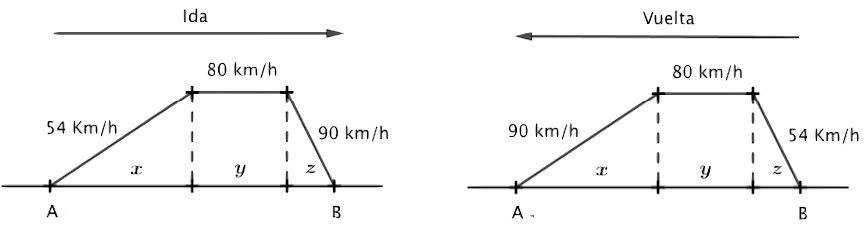
\includegraphics[width=.9\textwidth]{img-ecc/ecc06.png}
\end{figure}

\vspace{2mm} Suponiendo que el vehículo viaja a $v$ constante: $v=\frac s t \to t=\frac s v$. A la ida $t_{ida}=t_{x,s}+t_{y,n}+t_{z,b}$, a la vuelta $t_{vuelta}=t_{x,b}+t_{y,n}+t_{z,s}$, donde los subíndices $\; x,y,z\; $ indican los tramos que circula el coche a distintas velocidades y $\; s,n,b\; $ indican los tramos de `subida', `normal' y `bajada', respectivamente.
	
\vspace{2mm} La traducción del enunciado al leguaje algebraico conduce al sistema:
	
\vspace{2mm} $\begin{cases} x+y+z&=192\\ \frac{x}{54} + \frac{y}{80}+\frac{z}{90}&=2.5 \\ \frac{x}{90}+\frac{y}{80}+\frac{z}{94}&=2.75   \end{cases} \; \; $
	
\vspace{2mm} Lo más cómodo es multiplicar las ecuaciones 2 y 3 por el mcm de los denominadores (2160, en este caso) y conseguir un sistema sin denominadores que, resolviendo por Gauss tiene por solución única (\textbf{SCD}):
	
\vspace{2mm} $\boldsymbol{x=31.725 \; km; \; y= 94.800 \; km; \; z= 65.465 \; km}$, con lo que \textbf{la longitud de camino llano es de} $\boldsymbol{94.8 \; km}$.

\end{miejercicio}

\begin{miejercicio}
. Un tendero invierte 125 \euro $\,$ en la compra de una partida de manzanas. Desecha 20 kg por defectuosas y vende el resto, aumentando 0,40 \euro $\,$ cada kilo sobre el precio de compra, por 147 \euro. ?`Cuántos kilogramos compró?

\rule{250pt}{0.1pt}

\begin{figure}[H]
	\centering
	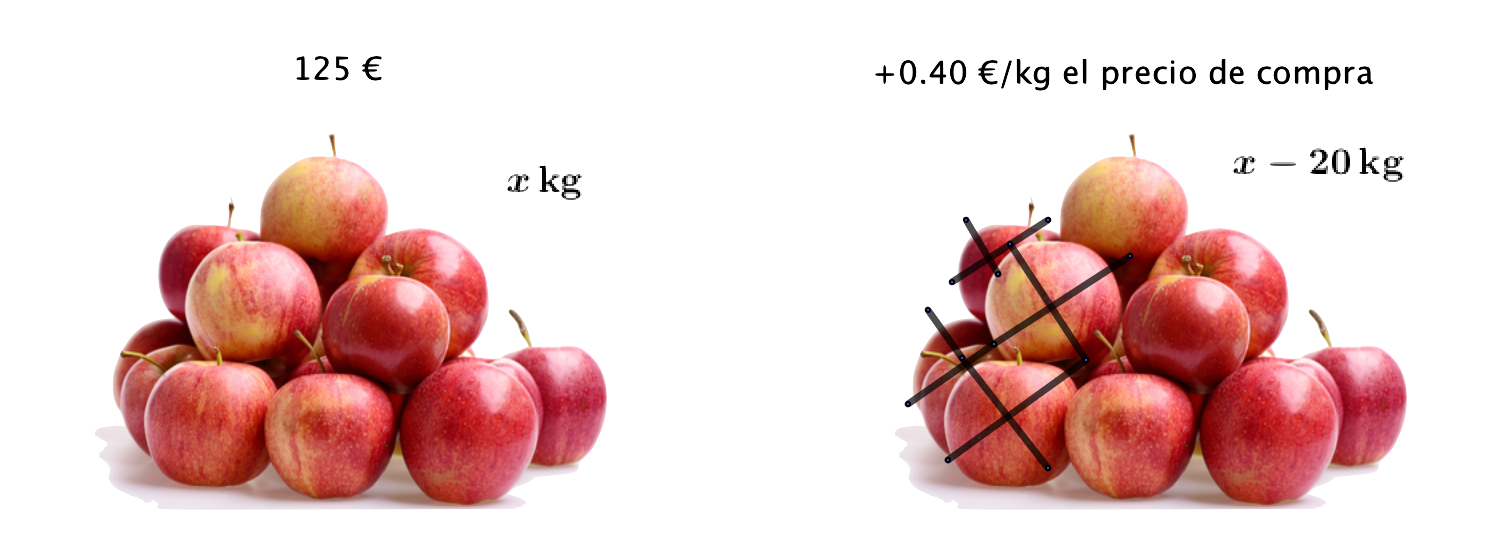
\includegraphics[width=.8\textwidth]{img-ecc/ecc04.png}
\end{figure}
Llamamos $ \ x \ $ a la cantidad de manzanas que compra el tendero inicialmente.

\vspace{2mm} Precio de compra: $\ \dfrac{125}{x}$ \euro/kg, precio de venta: $\ \dfrac{125}{x}+0.40$ \euro/kg. Vendemos un total de $\ x-20$ kg de manzanas. Recaudaremos:

\vspace{2mm} $(x-20)\cdot \left( \dfrac{125}{x}+0.40 \right) = 147 \ \to \ (125+0.4x)(x-20)=147 x \ \to \ 0.4x^2-30x-2500=0$

\vspace{2mm} Soluciones: $ \ x=-50\, , $ no aceptable en el contexto del problema y $\ x=125$, solución que no anula el denominador de nuestra ecuación racional y sí es aceptable.

\vspace{2mm} \textbf{Luego el tendero compra 125 kg de manzanas}.

\vspace{2mm} Comprobación: 125 kg de manzanas le cuestan 125 \euro. Cada kg le ha costado 1 \euro, el precio de compra es de 1 \euro/kg. Si se le estropean 20 kg, le quedan 125-20=105 kg de manzanas que venderá a 1+0.40=1.40 \euro/kg, por lo que recaudará 105$\cdot$1.40$=$147 \euro.

\end{miejercicio}

\begin{miejercicio}
. Dos grifos llenan un depósito de 1500 litros en una hora y doce minutos. Manando por separado, el primero tardaría una hora más que el segundo. ?`Cuánto tardaría en llenar el depósito cada grifo por separado?

\rule{250pt}{0.1pt}

\begin{figure}[H]
	\centering
	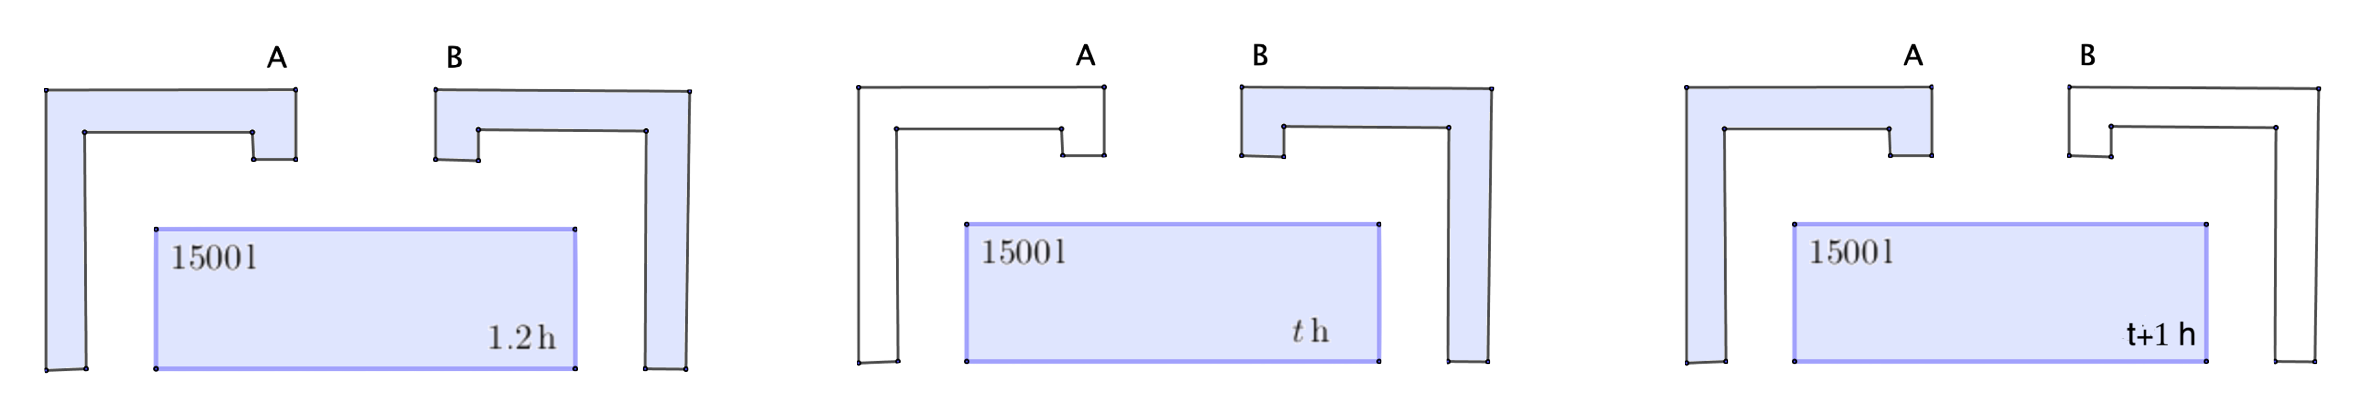
\includegraphics[width=1\textwidth]{img-ecc/ecc03.png}
\end{figure}


Entre los dos grifos vierten 1500 litros en 1.2 horas (1h y 12 min). Como el primero tarda una hora más que el segundo, llamaremos $t$ al tiempo que tardaría el segundo grifo en llenar el depósito con lo que, evidentemente, el primero lo haría en $t+1$ horas.

\vspace{2mm} El primer grifo vierte $\dfrac {1500}{t+1}$ litros cada hora, el segundo $\dfrac {1500} {t} $ l/h. Ambos a la vez vertirán $\dfrac{1500}{1.2}$ l/h. 
$\quad \Rightarrow \quad  \dfrac {1500} {t} +\dfrac {1500}{t+1} = \dfrac{1500}{1,2} \ \to \ \dfrac {1} {t} +\dfrac {1}{t+1} = \dfrac{1}{1,2} \quad MCM:\ 1,2t(t+1)$

\vspace{2mm} $1.2 (t+1) \ + \ 1.2t \ = \ t(t+1) \ \to \ 2.4t+1.2=t^2+t \ \to \ t^2 -1.4 t-1.2=0 \begin{cases} \ t=-0.6\\ \ t=2\end{cases}  $ 

\vspace{2mm} Puesto que la solución de que el grifo B llene el depósito en -0.6 horas (36 min antes de abrirlo)  carece de sentido, la solución es que \textbf{el grifo B tarda 2 horas} en llenar el depósito si está abierto él solo y que \textbf{el grifo A tardará 2+1=3 h} en llenarlo  si solo se abre A.
\end{miejercicio}


%%%%%%%%%%%%%%%%%%%%%%%%%%%%%%%%%%%%%%%%%%%%%%%%%
\vspace{1cm}
\section{Ejercicios}
\begin{tikzpicture}
	\fill [left color=red!50, right color=teal!50] (0,0) rectangle (3.5,.1);
	\fill [left color=teal!50, right color=blue!50] (3.5,0) rectangle (7.5,.1);
	\end{tikzpicture}
\vspace{0.5cm}

%*******
\begin{mipropuesto}
. $a)\ \dfrac{x(x-1)}{2}+\dfrac{(2x-1)^2}{3}=x+1\dfrac x 2; \qquad b) \ \ x(x+4)-5=\dfrac{x(x-1)}{3}$
\end{mipropuesto}
\vspace{-8mm}
\begin{flushright}
	\begin{footnotesize} \textcolor{gris}{\rotatebox{180}{ $a)\ \ x=2 \ \vee \ x=-2/11;\qquad b)\ \ x=1\ \vee \ x=-15/2$ }}	\end{footnotesize}
\end{flushright}

%*******
\begin{mipropuesto}
. $a)\ \ 2x^4-9x^2-5=0;\qquad b)\ \ 	(1-2x^2)^2+3x=2(x+2)^2+2$
\end{mipropuesto}
\vspace{-8mm}
\begin{flushright}
	\begin{footnotesize} \textcolor{gris}{\rotatebox{180}{ $a)\ \ \ x=\pm \sqrt{5};\qquad b)\ \ x=\frac{9\pm \sqrt{153}}{4}$ }}	\end{footnotesize}
\end{flushright}

%*******
\begin{mipropuesto}
. $a)\ \ x^3-4x^2-7x+10=0;\quad b)\ \ x^5+x^4-9x^3-9x^2=0;\quad c)\ \ 6x^4+7x^3+6x^2-1=0$	
\end{mipropuesto}
\vspace{-8mm}
\begin{flushright}
	\begin{footnotesize} \textcolor{gris}{\rotatebox{180}{ $a)\ \ 1,-1,-3/2;\quad b)\ \ 0,1,3,-3;\quad c)\ \ -1/2, -1/3$ }}	\end{footnotesize}
\end{flushright}

%*******
\begin{mipropuesto}
. $a)\ \ \dfrac{48}{5(x-3)}-\dfrac{33}{5(x+2)}+x^2+6=0;\qquad b)\ \ \dfrac{1}{x^2-5x+6}+\dfrac{1}{x^2-4x+3}=\dfrac{1}{x^2-3x+2}$	
\end{mipropuesto}
\vspace{-8mm}
\begin{flushright}
	\begin{footnotesize} \textcolor{gris}{\rotatebox{180}{ $a)\ \ 1,\pm \sqrt{3}; \qquad b)\ \ 0\, ,  \quad MCM=(x-1)(x-2)(x-3)$ }}	\end{footnotesize}
\end{flushright}

%*******
\begin{mipropuesto}
. $a)\ \ 17+\sqrt{169-x^2}=x;\quad b)\ \ \sqrt{2x-1}=\sqrt{3x-2}+\sqrt{1-x};\quad c)\ \ \sqrt{3x+3}-1=\sqrt{8-2x}$	
\end{mipropuesto}
\vspace{-8mm}
\begin{flushright}
	\begin{footnotesize} \textcolor{gris}{\rotatebox{180}{ $a)\ \ \nexists x;\quad b)\ \ x=1;\quad c)\ \ x=2$ }}	\end{footnotesize}
\end{flushright}

%*******
\begin{mipropuesto}
. $a)\ \ \dfrac{4^{x-1}}{2^{x+3}}=17;\qquad b)\ \ 2^{x-1}+2^x+\dfrac{1}{2^x}=\dfrac 7 2;\qquad c)\ \ 8^{x+1}+2^{3x-1}=\dfrac{17}{16}$	
\end{mipropuesto}
\vspace{-8mm}
\begin{flushright}
	\begin{footnotesize} \textcolor{gris}{\rotatebox{180}{ $a)\ \ x=\log_217+5;\quad b)\ \ x=1 \ \vee \ x= -\log_23;\quad c)\ \ x=-1$ }}	\end{footnotesize}
\end{flushright}

%*******
\begin{mipropuesto}
. $a)\ \ \ln(x-3)+\ln(x+1)=\ln 3+ \ln(x-1);\qquad b)\ \ (x-1)\log 3^{x+1}=3\log 3;$

$c)\ \ \log(x^2+3x+36)=1+\log(x+3)$ 	
\end{mipropuesto}
\vspace{-8mm}
\begin{flushright}
	\begin{footnotesize} \textcolor{gris}{\rotatebox{180}{ $a)\ 5;\qquad b)\ 2;\qquad c)\ 1\, , \ 6$ }}	\end{footnotesize}
\end{flushright}

%*******
\begin{mipropuesto}
. $a)\ \ \left| \dfrac{x+2}{5} \right|=x-2;	\qquad \qquad  \qquad  b)\ \ |x^2-x|=|1-x^2|$
\end{mipropuesto}
\vspace{-8mm}
\begin{flushright}
	\begin{footnotesize} \textcolor{gris}{\rotatebox{180}{ $a)\ 4/3;\qquad b)\ 1,\ -1/2$ }}	\end{footnotesize}
\end{flushright}

%*******
\begin{mipropuesto}
. $a)\ \ \begin{cases}	\ \dfrac 3 x - \dfrac x y &=0\\ \ 2x-y&=3 \end{cases};\qquad  b)\ \ \begin{cases} \ \dfrac{x-2}{3}-\dfrac{y-4}{2}=1  \\ \  \dfrac{2}{x-3}=\dfrac{4}{y-2} \end{cases}; \qquad c)\ \ \begin{cases} \ y+2x=x^2\\\ x+y=6 \end{cases} $
\end{mipropuesto}
\vspace{-8mm}
\begin{flushright}
	\begin{footnotesize} \textcolor{gris}{\rotatebox{180}{ $a)\ \ x=3,\ y=3; \qquad  b)\ \ x=7/2,\ y=3; \qquad c)\ \ x=3,\ y=3 \ \ \wedge \ \ x=-2,\ y=8 $ }}	\end{footnotesize}
\end{flushright}

%*******
\begin{mipropuesto}
. 	$a)\ \ \begin{cases} \ 2x-y=9 \\ \ \sqrt{x+y}+y=x \end{cases} ; \qquad \qquad \qquad b) \ \ \begin{cases}  \ x-2y=1\\ \ \sqrt{x+y}-\sqrt{x-y}=2 \end{cases}$
\end{mipropuesto}
\vspace{-8mm}
\begin{flushright}
	\begin{footnotesize} \textcolor{gris}{\rotatebox{180}{ $a)\ \ x=6,\ y=3;\qquad b)\ \ x=17,\ y=8$ }}	\end{footnotesize}
\end{flushright}

%*******
\begin{mipropuesto}
. $a)\ \begin{cases} \ e^x\, e^y=e^9 \\ \ 2^x/4^y=1/8 \end{cases}; \quad b)\ \begin{cases} \ \log(x^2+y)-\log(x-2y)=1 \\ \ 5^{x+1}=25^{y+1} \end{cases};\quad c)\ \begin{cases} \ x^2-y^2=11\\ \ \log x -\log y=1 \end{cases}$
\end{mipropuesto}
\vspace{-8mm}
\begin{flushright}
	\begin{footnotesize} \textcolor{gris}{\rotatebox{180}{ $a)\ x=5,\ y=4;\quad b)\ x=3,\ y=1;\quad c)\ x=10/3,\ y=1/3$ }}	\end{footnotesize}
\end{flushright}

%*******
\begin{mipropuesto}
. $a)\ \left\{\begin{array}{rrr} x+y-z&=&2\\ 2x-2y+3z&=&1 \\ x+2y-z&=&4 \end{array}	\right. ; \quad
b)\ \left\{ \begin{array}{rrr} x+y+x&=&3 \\ -x+2y+z&=&5 \\ x+4y+3z&=&1 \end{array} \right.; \quad
c)\ \left\{  \begin{array}{rrr} x+y+3z&=&2 \\ 2x+3y+4z&=&1 \\ 2x+y+8z&=&7 \end{array} \right.$
\end{mipropuesto}
\vspace{-8mm}
\begin{flushright}
	\begin{footnotesize} \textcolor{gris}{\rotatebox{180}{ $a) \ SCD: \ x=1, y=2, z=1;\quad b)\ SI;\quad c)\ SCI:\ x=5-5\lambda, y=2\lambda-3, z=\lambda$ }}	\end{footnotesize}
\end{flushright}

%*******
\begin{mipropuesto}
.  Determina los valores de $a$ y $b$ para que $x=2$ e $y=3$ sean solución del sistema: 

$\quad \left\{ \begin{array}{rrrr}  \dfrac 5 2 x&-ay &=&3 \\   -\dfrac 1 3 x &+ ay&=&b	 \end{array} \right.$
\end{mipropuesto}
\vspace{-8mm}
\begin{flushright}
	\begin{footnotesize} \textcolor{gris}{\rotatebox{180}{ $a=8/3,\ b=22/8$ }}	\end{footnotesize}
\end{flushright}


%*******
\begin{mipropuesto}
. Resuelve $\qquad \begin{cases} \ (x+1)\, (y+1) = 9 \\ \ (x+2)\, (y-3)=-4 \end{cases}$
\end{mipropuesto}
\vspace{-8mm}
\begin{flushright}
	\begin{footnotesize} \textcolor{gris}{\rotatebox{180}{ $x=2,\ y=-13$ }}	\end{footnotesize}
\end{flushright}
\vspace{-8mm}
\begin{flushright}
	\begin{scriptsize} \textcolor{gris}{\rotatebox{180}{ Desarrolla en iguala $xy$ en ambas ecuaciones, luego despeja una incóginta y sustituye  en cualquier ecuación.}}	\end{scriptsize}
\end{flushright}


%*******
\begin{mipropuesto}
. Dos trabajadores realizan un trabajo en 12 días si lo hacen conjuntamente. Si lo hacen por separado, uno de ello tarda 10 días más en acabarlo que el otro. ?`Cuántos días necesita cada trabajador para realizar la faena por separado?
\end{mipropuesto}
\vspace{-8mm}
\begin{flushright}
	\begin{footnotesize} \textcolor{gris}{\rotatebox{180}{ 30 y 20 días. }}	\end{footnotesize}
\end{flushright}




%%%%%%%%%%%%%%%%%%%%%%%%%%%%%%%%%%%%%%%%%%%%%%%%%

\newpage

$\qquad$


\begin{adjustwidth}{50pt}{250pt}
\begin{cuadro-naranja}
\textbf{\huge{Problemas $\boldsymbol{+}$}}\normalsize{$\, $}
\end{cuadro-naranja}	
\end{adjustwidth}



\vspace{5mm}
\begin{enumerate}[\textbf{P$\boldsymbol +$} 1. ]
\item	$x^{\sqrt{x}}\ = \ x\, \sqrt{x}$

\vspace{-6mm}
\begin{flushright}
\begin{footnotesize} \textcolor{gris}{\rotatebox{180}{ Escribe el segundo miembro en forma de petencia racional de x e identifica exponentes: $\ x=9/4$ }}	\end{footnotesize}
\end{flushright}

\item	$x+y=4;\quad xy=5 \quad \to \quad \dfrac 1 x + \dfrac 1 y = ?$

\vspace{-6mm}
\begin{flushright}
\begin{footnotesize} \textcolor{gris}{\rotatebox{180}{ 4/5 }}	\end{footnotesize}
\end{flushright}

\item	$	\begin{cases} \ x^2+y^2&=30 \\ \ x+y&= 10 \end{cases} \to \ \ $ Calcula $\ xy$

\vspace{-6mm}
\begin{flushright}
\begin{footnotesize} \textcolor{gris}{\rotatebox{180}{ Cuadrado de un binomio suma. $\ \ xy=35$ }}	\end{footnotesize}
\end{flushright}

\item	Si $x+y=7$ y $x^3+y^3=133$, ?`qué vale $xy$?

\vspace{-6mm}
\begin{flushright}
\begin{scriptsize} \textcolor{gris}{\rotatebox{180}{ $x^3+y^3=(x+y)(x^2-xy+y^2) \ \to \ x^2-xy+y^2$ conocido; $x^2-xy+y^2=x^2+2xy+y^2\ - \ 3xy$. Sol. $xy=25$ }}	\end{scriptsize}
\end{flushright}


\item	En un instituto de 300 estudiantes, cada estudiante lee 5 periódicos y cada periódico es leído por 60 estudiantes. ?`Cuántos periódicos hay?

\vspace{-6mm}
\begin{flushright}
\begin{footnotesize} \textcolor{gris}{\rotatebox{180}{ Es importante el número de lecturas. Llama $n=$ al número de periódicos en el centro. $\ n=25$ }}	\end{footnotesize}
\end{flushright}

\item	Una madre es 21 años mayor que su hijo y entro de 6 años la edad de la madre quintuplicará la del hijo. ?`Dónde está el padre?

\vspace{-6mm}
\begin{flushright}
\begin{footnotesize} \textcolor{gris}{\rotatebox{180}{ Junto a la madre. \textcolor{gris}{(hijo=-3/4 año =-9 meses)} }}	\end{footnotesize}
\end{flushright}

\item	$3\log_8x=\log_4(x+6)\, . \ $ Calcula la suma de todas las soluciones de esta ecuación.

\vspace{-6mm}
\begin{flushright}
\begin{footnotesize} \textcolor{gris}{\rotatebox{180}{ Sol 3 (comprueba qué soluciones son válidas) }}	\end{footnotesize}
\end{flushright}

\item	$\log_{\sqrt{2}}\sqrt{x}+\log_2x+\log_4x^2+\log_8x^3+\log_{16}{x^4}=40$

\vspace{-6mm}
\begin{flushright}
\begin{footnotesize} \textcolor{gris}{\rotatebox{180}{ Escribe todos los logaritmos en la misma base. $\ x=64$ }}	\end{footnotesize}
\end{flushright}

\item $\begin{cases} \ \log_xy+\log_yx=17/4 \\ \ xy=288\sqrt{3} \end{cases}$

\vspace{-4mm}
\begin{flushright}
\begin{footnotesize} \textcolor{gris}{\rotatebox{180}{ $x=144 \leftrightarrow y=2\sqrt{3} \  \vee \  x=2\sqrt{3} \leftrightarrow y=144\quad $ Ecuaciones simétricas $\leftrightarrow$ soluciones simétricas.  }}	\end{footnotesize}
\end{flushright}
\vspace{-6mm}
\begin{flushright}
\begin{footnotesize} \textcolor{gris}{\rotatebox{180}{ Trabaja la primera ecuación, usa solo $\log_x$ y resuelve (puedes necesitar un cambio de variable) }}	\end{footnotesize}
\end{flushright}


\item	$\left| \, 3x-|1-2x| \, \right|=2$

\vspace{-6mm}
\begin{flushright}
\begin{footnotesize} \textcolor{gris}{\rotatebox{180}{ $x=1 \, ; \ \wedge \ x=-1/5$ }}	\end{footnotesize}
\end{flushright}

\item	$\sqrt[3]{4x-1}=x-4$

\vspace{-6mm}
\begin{flushright}
\begin{footnotesize} \textcolor{gris}{\rotatebox{180}{ Eleva al cubo. $\quad x=7$ }}	\end{footnotesize}
\end{flushright}


\item	$abx^2-(a+b)x+1=0$

\vspace{-6mm}
\begin{flushright}
\begin{footnotesize} \textcolor{gris}{\rotatebox{180}{ $x=1/a \ \wedge \ x=1/b$ }}	\end{footnotesize}
\end{flushright}

\item	$(a+b)x^2=a-bx$

\vspace{-6mm}
\begin{flushright}
\begin{footnotesize} \textcolor{gris}{\rotatebox{180}{ $x=-1 \ \wedge \ x=\dfrac{a}{a+b}$  }}	\end{footnotesize}
\end{flushright}

\item	$(x-a)^2+x(x-b)=8b^2-x(2a-b)+a^2$

\vspace{-6mm}
\begin{flushright}
\begin{footnotesize} \textcolor{gris}{\rotatebox{180}{ $x=\pm 2b$ }}	\end{footnotesize}
\end{flushright}


\item	Resuelve: $a)\ \ \dfrac{1}{a^2+\dfrac{1}{a+1}}=a-1\, ; \qquad b)\ \ \sqrt{x+\sqrt{4x+\sqrt{16x+\sqrt{64x+5}}}}-\sqrt{x}=1 $

\vspace{-4mm}
\begin{flushright}
\begin{footnotesize} \textcolor{gris}{\rotatebox{180}{ a) bicuadrada, sol. $x=\pm \sqrt{2}\qquad $ b) aisla y eleva al cuadrado repetidamente, sol $\ \ x=1/16$ }}	\end{footnotesize}
\end{flushright}


\item	El mito de Sísifo

\begin{small} \emph{En la mitología griega, Sísifo fue fundador y rey de Éfira, más tarde conocida como Corinto. Era uno de los siete hijos de Eolo y Enareta, y esposo de Mérope, hija de Atlante. Sísifo era un ejemplo de rey impío, pues es conocido por su castigo: empujar cuesta arriba por una montaña una piedra que, antes de llegar a la cima, volvía a rodar hacia abajo, repitiéndose una y otra vez el frustrante y absurdo proceso. El término ``trabajo de Sísifo'', que se utiliza en la actualidad para describir un trabajo duro que debe hacerse una y otra vez, tiene su origen en el castigo de Sísifo} \end{small}

\begin{multicols}{2}
	\begin{figure}[H]
	\centering
	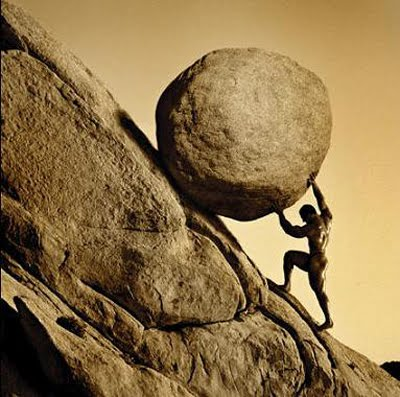
\includegraphics[width=.4\textwidth]{img-ecc/ecc16.jpeg}
\end{figure}

Sísifo debe llevar cada día una piedra a la cima de la montaña. El primer día tarda 7 horas en subir y bajar.

\vspace{2mm} La tarea es pesada y, cada día, tarda el doble que el anterior en subir y la mitad que el anterior en bajar.

\vspace{2mm} Si emplea 8 horas en subir y bajar la piedra el segundo día, ?`cuántas horas tardará en subir y bajar el tercer día?	
	\end{multicols}


\vspace{-6mm}
\begin{flushright}
\begin{footnotesize} \textcolor{gris}{\rotatebox{180}{ El tercer día tarda 13 horas. }}	\end{footnotesize}
\end{flushright}



\end{enumerate}

%%%%%%%%%%%%%%%%%%%%%%%%%%%%%%%%%%%%%%%%%%%%%%%%%
\newpage
\begin{small}
\section{Resumen del tema}
\begin{tikzpicture}
	\fill [left color=red!50, right color=teal!50] (0,0) rectangle (3.5,.1);
	\fill [left color=teal!50, right color=blue!50] (3.5,0) rectangle (7.5,.1);
	\end{tikzpicture}
\vspace{1cm}

\begin{myblock}{Resumen: \emph{``Ecuaciones y sistemas''}}

\vspace{2mm} \textbf{\underline{ECUACIONES}}:

\vspace{4mm} $\triangleright \ \ $ \textbf{Ecuaciones de primer grado}: $\ ax+b = 0   \ \to \ x=-b/a$

\vspace{2mm} Algoritmo:  quitar paréntesis y/o denominadores, trasposición de términos, agrupar y despejar.

\vspace{2mm} Pueden tener 1 solución única, infinitas soluciones o ninguna solución.


\vspace{4mm} $\triangleright \ \ $ \textbf{Ecuaciones de segundo grado}:  $ax^2 + bx + c = 0  \ to \  $ fórmula general  

\vspace{2mm} Ecuaciones incompletas: factor común o despejar

\vspace{4mm} $\triangleright \ \ $ \textbf{Ecuaciones reducibles a 2$^o$ grado} (bicuadradas):  $ax^{2n}+bx^n+c=0  \ \to \ $  el cambio: $x^n=t$ la convierte en una ecuación de segundo grado. Acordarse de deshacer el cambio.

\vspace{4mm} $\triangleright \ \ $ \textbf{Ecuaciones polinómicas}:  (grado mayor o igual a 3) $\to$ Factorizar por Ruffini (esto permite encontrar las soluciones enteras o racionales).

\vspace{4mm} $\triangleright \ \ $ \textbf{Ecuaciones racionales}: (cocientes de polinomios, aparecen x en el denominador). Para eliminar los denominadores hay que multiplicar TODA la ecuación por el MCM de los DENOMINADORES.

\vspace{2mm} \textcolor{red}{$\boldsymbol{\boxed{ \ ! \ }} $}  $\ $ Hay que COMPROBAR SIEMPRE LAS SOLUCIONES obtenidas en la ecuación de partida.

\vspace{4mm} $\triangleright \ \ $ \textbf{Ecuaciones irracionales}: (con la x bajo el símbolo radical): Tendremos que aislar la/las raíz/raices en un miembro de la ecuación y elevar al cuadrado. El proceso puede necesitar de repetición.

\vspace{2mm} \textcolor{red}{$\boldsymbol{\boxed{ \ ! \ }} $}  $\ $ Hay que COMPROBAR SIEMPRE LAS SOLUCIONES obtenidas en la ecuación de partida.

\vspace{4mm} $\triangleright \ \ $ \textbf{Ecuaciones exponenciales}: La incógnita está en el exponente. Podremos usar propiedades de las potencias, logaritmos, a veces será necesario un cambio de variable (acordarse al final de deshacerlo)

\vspace{4mm} $\triangleright \ \ $ \textbf{Ecuaciones logarítmicas}: la x está dentro de algún logaritmo. Usaremos las propiedades de los logaritmos.

\vspace{2mm} \textcolor{red}{$\boldsymbol{\boxed{ \ ! \ }} $}  $\ $ Hay que COMPROBAR SIEMPRE LAS SOLUCIONES obtenidas en la ecuación de partida.

\vspace{4mm} $\triangleright \ \ $ \textbf{Ecuaciones con valor absoluto}: la x aparece dentro del valor absoluto o módulo.$\ $ \textcolor{red}{$\boldsymbol{\boxed{ \ ! \ }} $}  $\ $ Si se resuelven con rigor, estudiando signos, no hay problema. Pero si usamos que $|x|=a\ \leftrightarrow \  x=a  \ \vee \   x=-a$ en expresiones complicadas, habrá que COMPROBAR SIEMPRE LAS SOLUCIONES obtenidas en la ecuación de partida.


\vspace{6mm} \textbf{\underline{SISTEMAS DE ECUACIONES}}:  Sustitución, reducción, igualación. Gauss (SEL).
	
\end{myblock}
\end{small}







\begin{comment}

%%%%%%%%%%%%%%%%%%%%%%%%%%%%%%%%%%%. SECCIONES

PROBLEMAS DE ENUNCIADO *****************************************************

\begin{figure}[H]
	\centering
	
\includegraphics[width=0.35\textwidth]{img-pol/pol05.png}
\end{figure}




\chapter{texto}
\begin{tikzpicture}
	\fill [left color=red!50, right color=teal!50] (0,0) rectangle (6.5,.2);
	\fill [left color=teal!50, right color=blue!50] (6.5,0) rectangle (11.5,.2);
	\end{tikzpicture}

\vspace{1cm}
\section{texto}
\begin{tikzpicture}
	\fill [left color=red!50, right color=teal!50] (0,0) rectangle (3.5,.1);
	\fill [left color=teal!50, right color=blue!50] (3.5,0) rectangle (7.5,.1);
	\end{tikzpicture}
\vspace{0.5cm}

\subsection{texto}
\begin{tikzpicture}
	\fill [left color=red!50, right color=teal!50] (0,0) rectangle (3.5,.01);
	\fill [left color=teal!50, right color=blue!50] (3.5,0) rectangle (7.5,.01);
	\end{tikzpicture}
\vspace{0.5cm}


%%%%%%%%%%%%%%%%%%%%%%%%%%%%%%%%%%%. \begin{ ------>. 
detsacado;  cuadro-naranja;  cuadro-gris;  miejercicio (solución extensa);  mipropuesto (solución corta y fuera del cuadro)

%%%%%%%%%%%%%%%%%%%%%%%%%%%%%%%%%%%. CURIOSIDAD
\vspace{1cm}
\color{ForestGreen!80}
\rule{250pt}{0.2pt}
Texto
\vspace{-8mm}
\begin{flushright}
\rule{250pt}{0.2pt}		
\end{flushright}	
\color{black}
\end{comment} %
\chapter{Inecuaciones y sistemas}
\begin{tikzpicture}
	\fill [left color=red!50, right color=teal!50] (0,0) rectangle (6.5,.2);
	\fill [left color=teal!50, right color=blue!50] (6.5,0) rectangle (11.5,.2);
	\end{tikzpicture}


\vspace{5mm}
\begin{adjustwidth}{40pt}{40pt}
\begin{cuadro-gris}

	\begin{multicols}{2}
	
	$\triangleright \quad$  Inecuaciones con una incógnita: 
	
	$\qquad $--- lineales  
	
	$\qquad $--- no lineales.	
	
	$\triangleright \quad$  Sistemas de inecuaciones con una incógnita.
	
	$\triangleright \quad$ Inecuaciones y sistemas lineales con dos incógnitas.
	\end{multicols}
	
\end{cuadro-gris}
\end{adjustwidth}

\vspace{1cm}
\begin{definition}
.	Una inecuación es una desigualdad algebraica en la que sus dos miembros aparecen ligados por uno de estos signos $\ <\, , \ \ >\, , \ \ \leqslant \, \ \ \geqslant$. 

\vspace{2mm} La solución de una inecuación es el conjunto de valores de la variable que verifica la inecuacíón, serán intervalos de la recta real.
\end{definition}
\vspace{5mm}

\begin{myexampleblock}{Historia de las inecuaciones}

\vspace{2mm} No se sabe exactamente el origen de las inecuaciones pero se cree que se originaron poco después de las ecuaciones (1700aC. – 1700dC.) debido al surgimiento de un problema en el cual la respuesta podía contener un grupo de números.

\vspace{2mm} Una inecuación es una expresión matemática la cual se caracteriza por tener los signos de desigualdad.

\vspace{2mm} La notación $\ a < b \ $ significa que $a$ es menor que $b$ y la notación $\ a > b \ $ quiere decir que $a$ es mayor que $b$. Estas relaciones son conocidas con el nombre de desigualdades estrictas, contrastando con $ \ a \leqslant b\ $ ($a$ es menor o igual que $b$  y $\ a \geqslant b\ $ ($a$ es mayor o igual que $b$).

\vspace{2mm} La notación $\ a >> bº $ quiere decir que $a$ ``es mucho mayor'' que $b$. 
	
\end{myexampleblock}


\vspace{5mm}
\begin{theorem}
.	Hay que tener en cuenta que:

\begin{itemize}
\item Si a los dos miembros de una inecuación se les suma o se les resta un mismo número, la inecuación resultante es equivalente a la dada.
\item Si a los dos miembros de una inecuación se les multiplica o divide por un mismo número positivo, la inecuación resultante es equivalente a la dada.
\item Si a los dos miembros de una inecuación se les multiplica o divide por un mismo número negativo, la inecuación resultante cambia de sentido y es equivalente a la dada.
\end{itemize}
\end{theorem}

\vspace{5mm}

\begin{multicols}{2}
	\begin{destacado}
	\vspace{2mm}$2<5 \ \to \ 2+7<5+7\Rightarrow 9<12$

	$2<5 \ \to \ 2\cdot 3 < 5\cdot 3 \Rightarrow 6<15$

	$2<5 \ \to \ 2\cdot (-4) < 5\cdot (-4) \Rightarrow -8 \boldsymbol >-20$

	\vspace{2mm}Al multiplicar (dividir) toda una una inecuación por un número negativo, \emph{el sentido de la desigualdad \textbf{cambia}}: $<$ se convierte en $>$, $\ \leqslant$ se convierte en $\geqslant$, $\ >$ se convierte en $<$ y $\ \geqslant$ en $\leqslant$.
	\vspace{2mm}
	\end{destacado}

	\begin{figure}[H]
		\centering
		\includegraphics[width=0.45\textwidth]{img-ecc/ecc10.png}
	\end{figure}
\end{multicols}




\vspace{1cm}
\section{Inecuaciones con una incógnita}
\begin{tikzpicture}
	\fill [left color=red!50, right color=teal!50] (0,0) rectangle (3.5,.1);
	\fill [left color=teal!50, right color=blue!50] (3.5,0) rectangle (7.5,.1);
	\end{tikzpicture}
\vspace{0.5cm}

\subsection{Inecuaciones lineales con una incógnita}
\begin{tikzpicture}
	\fill [left color=red!50, right color=teal!50] (0,0) rectangle (3.5,.01);
	\fill [left color=teal!50, right color=blue!50] (3.5,0) rectangle (7.5,.01);
	\end{tikzpicture}
\vspace{0.5cm}

\begin{definition}

Tienen la forma: $\qquad ax+b \ < 0 \ (\leqslant, >, \geqslant)\  , \ \text{ con } a,b\in \mathbb R,\ a\neq 0$
	
\end{definition}

\begin{theorem}

Procedimiento de resolución:

\begin{itemize}
\vspace{-2mm} \item Quitar paréntesis.
\vspace{-2mm} \item Quitar denominadores.
\vspace{-2mm} \item Trasponer términos.
\vspace{-2mm} \item Reducir a términos semejantes.
\vspace{-2mm} \item Despejar (cuidado: si hay que multiplicar --dividir-- por un número negativo, la desigualdad se invierte --cambia de sentido--)	
\end{itemize}
	
\end{theorem}

\begin{miejemplo}

	Resuelve $\qquad \dfrac 2 3 \left[ x-\left( 1-\dfrac{x-2}{3} \right) \right]+1\ <\ x$
	
\vspace{5mm} $\dfrac 2 3 \left[ x- 1+\dfrac{x-2}{3}  \right]+1\ <\ x
\ \to \ 
\dfrac 2 3 \left[ \dfrac{3x-3+x-2}{3}  \right]+1\ <\ x \ \to \ 
\dfrac 2 3 \left[ \dfrac{4x-5}{3}  \right]+1 \ \to $

\vspace{2mm} $\to \textcolor{red}{9\, }\cdot \dfrac{2(4x-5)}{9} + \textcolor{red}{9\, }\cdot 1 < \textcolor{red}{9\, }\cdot x \, ; \ \ \text{MCD: \textcolor{red}{9\, }} \ \to \ 2(4x-5)+9<9x\ \to 8x-10+9<9x \to $

\vspace{2mm}$\to \ 8x-9x<10-9 \ \to \ -x<1\, ;\quad  \text{ multiplicando por } (-1) \ \Rightarrow \ \boldsymbol{x>-1}$

\vspace{2mm} Solución: $\ \{ \forall x \in \mathbb R \, / \, \ x>-1 \}\ \longleftrightarrow \ \ \boldsymbol{]-1,+\infty[}$
\end{miejemplo}

\begin{miejercicio}

Resuelve: $\qquad 6\left( \dfrac{x+1}{8}-\dfrac{2x-3}{16} \right) \ \geqslant \ 3\left( \dfrac{3}{4}x-\dfrac 1 4 \right) - \dfrac 3 8 (3x-2)$

\rule{250pt}{0.1pt}	

\vspace{5mm} $\dfrac{6(x+1)}{8}-\dfrac{6(2x-3)}{16} \geqslant \dfrac{3(3x-1)}{4}-\dfrac{3(3x-2)}{8};\qquad MCM:16$

\vspace{2mm} $16\cdot \dfrac{6(x+1)}{8}-16\cdot \dfrac{6(2x-3)}{16} \geqslant 16\cdot \dfrac{3(3x-1)}{4}-16\cdot \dfrac{3(3x-2)}{8}$

\vspace{2mm} $12(x+1)-6(2x-3) \geqslant 12(3x-1)-6(3x-2) \ \to \ \cancel{12x}]+12-\cancel{12x}+18 \leqslant 36x-\cancel{12}-18x+\cancel{12}$

\vspace{2mm} $-36x+18x \geqslant -12-18 \ \to \ -18x \geqslant 30\, ; \ $ Multiplicando por $\, (-1)$:

\vspace{2mm} $18 \leqslant -30 \ \to \ x\leqslant 5/3\ \ $ Solución: $\ \{ \forall x \in \mathbb R \, / \, \ x \leqslant 5/3 \}\ \longleftrightarrow \ \ \boldsymbol{]-\infty,5/3]}$

\end{miejercicio}


\vspace{0.5cm}
\subsection{Inecuaciones no lineales con una incógnita}
\begin{tikzpicture}
	\fill [left color=red!50, right color=teal!50] (0,0) rectangle (3.5,.01);
	\fill [left color=teal!50, right color=blue!50] (3.5,0) rectangle (7.5,.01);
	\end{tikzpicture}
\vspace{0.5cm}

No es sencillo estudiar cuando una determinada expresión algebraica es mayor (o menor) a otra, pero resulta más sencillo estudiar cuado una determinada expresión es mayor (menor) que cero, cuando es positiva (o negativa), cuando cambia de signo (en algún momento ha de valer cero). Por ello esta será la estrategia principal que usaremos: \emph{llevar todo a un solo miembro de la inecuación y en el otro habrá un cero}, determinaremos cuando es cero el numerador y denominador de nuestra expresión (si los hay) y estudiaremos el signo que toma la expresión a estudio en cada una de las zonas que aparecerán. 

Para inecuaciones irracionales con radicales pares hay que exigir, además, que todos los radicandos sean no negativos ($\geqslant 0$). Las inecuaciones sobre valores absolutos serán más delicadas, veremos todo esto en ejemplos y ejercicios resueltos a continuación.

\vspace{5mm}
\begin{large}
$\triangleright \quad $ \textbf{Inecuaciones de segundo grado}	
\end{large}
\vspace{5mm}

\begin{miejemplo}

Resuelve la inecuación: $\qquad 6x^2 \geqslant 5x+6$

\vspace{5mm} $6x^2-5x-6\geqslant 0 \ \longrightarrow	 \ 6x^2-5x-6=0 \ \leftrightarrow \ x=3/2 \ \wedge \ x=-2/3$

\vspace{2mm} $6x^2-5x-6=6(x-3/2)(x+2/3)=2(x-3/2)3(x+2/3)=(2x-3)(3x+2)$

\vspace{2mm} Nuestra inecuación es: $\quad (2x-3)(3x+2) \geqslant 0	\, ; \ $ Sabemos que es cero en $-2/3$ y en $3/2$, por lo que dividiremos el eje real en 3 zonas (y dos puntos) en que estudiaremos el signo que toma nuestra expresión \textcolor{gris}{(números menores que -2/3, en -2/3, desde -2/3 hasta 3/2, en 3/2, números mayores que 3/2)}.

\begin{table}[H]
\centering
\begin{tabular}{c|c|c|c|c|c|}
 & $]-\infty,-2/3[$  & $x=-2/3$ & $]-2/3,3/2[$ & $x=3/2$ & $]3/2,+\infty$[ \\ \hline
2x-3 & $-$ & $-$ & $-$ & 0 & $+$ \\ \hline
3x+2 & $-$ & 0 & $+$  & $+$  & $+$  \\ \hline
(2x-3)(3x+2) & $+$  & 0 & $-$	 & 0 & $+$  \\ \hline
?`$6x^2-5x-6 \geqslant 0$? & Sí & Sí  & No & Sí & Sí \\ \hline
\end{tabular}
\end{table}

Los signos los obtenemos al sustituir un número cualquiera de la zona en cuestión en la expresión indicada; así, p.e. en la zona $]-\infty,-2/3[$ tomamos el valor $x=-1$, el factor $2x-3=2(-1)-3=-5<0$, es negativo, $\boldsymbol{-}$. El factor $3x+2=3(-1)+2=-1<0$, también lo es, por lo que el producto $(2x-3)(3x+2)$ será positivo, $\boldsymbol{+}$ en esta zona.

Solución: $\boldsymbol{]-\infty,-2/3]\cup[3/2,+\infty[}$

\end{miejemplo}

\begin{multicols}{2}

Gráficamente: 

$\ y=x^2-5x-6=0\ $ es una parábola que corta al eje $\mathcal OX$ en $A(3/2,0)$ y $B(-2/3,0)$.

Una vez representada se observa que la parábola es positiva ($y\geqslant 0$) en $\ ]-\infty,-2/3]\cup[3/2,+\infty[$
\begin{figure}[H]
		\centering
		\includegraphics[width=0.5\textwidth]{img-ecc/ecc11.png}
	\end{figure}	
\end{multicols}

\begin{miejercicio}

Resuelve: $\qquad a)\ \ x^2+4x+4\leqslant 0;\qquad \qquad b)\ \ x^2+1\leqslant x$

\rule{250pt}{0.1pt}

\vspace{5mm} $\triangleright \quad a)\ \ x^2+4x+4=0 \ \to \ x=-2$

\vspace{2mm} Tenemos un único punto, dará lugar a tres zonas: menores que -2, el número -2 y mayores que -2. En ellas estudiaremos el signo que toma $x^2+4x+4$. 

\vspace{2mm} Con una tabla similar a la anterior obtendríamos que $x^2+4x+4$ es positivo (mayor que cero) tanto para números mayores que -2 como para números menores que -2 y que vale 0 en x=-2, por lo que la solución buscada, cuando $x^2+4x+4\leqslant0$, cuando es negativa o cero es, únicamente, para x=2. Solución, $\boldsymbol{x=2}$

\vspace{2mm} Pero es más sencillo razonar: $x^2+4x+4=0 \leftrightarrow x=-1 \ \to \ x^2+4x+4=(x+2)^2$ que \textbf{siempre} es positivo o cero, por lo que será $x^2+4x+4=(x+2)^2\leqslant 0$ solamente en $\boldsymbol{x=-2}$

\vspace{2mm} Para la inecuación $x^2+4x+4<0$, la solución sería $\nexists x$, que no la hay. Si la inecuación fuese $x^2+4x+4\geqslant 0$, la solución sería todos los números reales, $\mathbb R$. Y si la inecuación hubiese sido $x^4+4x+4>0$, la solución sería $]-\infty,-2[	\cup ]-2,+\infty[$

\vspace{5mm} $\triangleright \quad b) \ \ x^2+1\leqslant x \ \to \ x^2-x+1 \leqslant 0 \quad $ Veamos cuando es cero:

\vspace{2mm} $x^2-x+1=0 \ \to \ x=\dfrac{1\pm \sqrt{(-1)^2-4\cdot 1 \cdot 1}}{2} \ \ \nexists\ $  

\vspace{2mm} $x^2-x+1$ nunca es cero, nunca pasa por el cero, luego o siempre será positivo o siempre negativo. Tomemos un número cualquiera, p.e. $x=0 \to \ 0^2+4\cdot 0 + 4=4 > 0\, . \ $ Esta expresión es \emph{siempre} positiva, por lo que $x^2-x+1\leqslant 0$ nunca. Solución: $\ \emptyset   \ $ (conjunto vacío).

\vspace{2mm} También podríamos haber hecho una tabla con una sola zona, $\mathbb R$, el signo en esta. zona lo obtenemos al sustituir cualquier número de esta zona en nuestra inecuación y comprobar que  p.e. $x=0 \to \ 0^2+4\cdot 0 + 4=4 > 0\, . \ $, por lo que la inecuación no tendría solución.

\end{miejercicio}

\vspace{5mm}
\begin{large}
$\triangleright \quad $ \textbf{Inecuaciones de grado superior a 2}	
\end{large}
\vspace{5mm}

Se tratan del mismo modo que las de segundo grado

\begin{miejercicio}

Resuelve $\qquad x^4-20x \ \geq \ x^3+16x^2$

\rule{250pt}{0.1pt}	

\vspace{5mm} Llevando todo a la izquierda: $\ \ x^4-x^3-16x^2-20x \ \leqslant \ 0$

\vspace{2mm} Sacando factor común y factorizando, $\ x(x-5)(x+2)^2 >0\ $ \textcolor{gris}{El factor $(x+2)^2$ siempre es positivo por lo que solo puede cambiar el signo a la izquierda y derecha del 0 y del 5, el -2 no alterará los signos, salvo que dará 0 en x=-2. De todos modos, como se trata de un ejercicio para ilustrar el método no lo tendremos en cuenta.}

\vspace{2mm} Buscamos los ceros que darán lugar a las zonas en que estudiaremos los signos de los factores: $\ x(x-5)(x+2)^2=0 \ \leftrightarrow \ x=0\ \wedge \ x=5 \ \wedge \ x=-2$

\begin{table}[H]
\centering
\begin{tabular}{c|c|c|c|c|c|c|c|}
 & $]-\infty,-2[$ & $-2$ & $]-2,0[$ & $0$ & $]0,5[$ & $5$ & $]5,+\infty[$ \\ \hline
$x$            & $-$ & $-$ & $-$ & 0 & $+$ & $+$ & $+$ \\ \hline
$x-5$          & $-$ & $-$ & $-$ & $-$ & $-$ & 0 & $+$ \\ \hline
$(x+2)^2$.     & $+$ & 0 & $+$ & $+$ & $+$ & $+$ & $+$ \\ \hline
$x(x-5)(x+2)^2$ & $+$ & 0 & $+$ & 0 & $-$ & 0 & $+$ \\ \hline
?`$x(x-5)(x+2)^2\geqslant 0$? & No & Sí & No & Sí & Sí & Sí & No \\ \hline
\end{tabular}
\end{table}
Solución: $\quad \boldsymbol{ \{-2\} \cup [0,5]}$

\vspace{2mm} Si la inecuación hubiese sido, por ejemplo, $x^2+20x<x^3+16x*2$, cuando se obtiene un resultado negativo (no cero), la solución sería $\ ]0,5[$
\end{miejercicio}


\vspace{5mm}
\begin{large}
$\triangleright \quad $ \textbf{Inecuaciones sobre fracciones algebraicas}	
\end{large}
\vspace{5mm}

En este tipo de inecuaciones aparecerá, como novedad, que si el cero procede de un factor del denominador, al no estar definida la división por cero en matemáticas, proporcionará un punto donde la fracción no existirá, por lo que jamás formará parte de la solución.


\begin{miejemplo}

Resuelve: $\qquad \dfrac{x-1}{3x+6}>0$	

\vspace{5mm} Ceros numerador: $\ x-1=0 \ \to \ x=1\, . \ $ Ceros denominador $\ 3x+6=0 \ \to \ x=-2 \, . \ $ Los números 1 y -2 dividen en eje real en tres zonas (menores que -2, entre -2 y 1, mayores que 1):

\begin{table}[H]
\centering
\begin{tabular}{c|c|c|c|c|c|}
 & $]-\infty,-2[$ & $x=-2$ & $]-2,1[$ & $x=1$ & $]1,+\infty[$ \\ \hline
$x-3$ & $-$ & $-$ & $-$ & $0$ & $+$ \\ \hline
$3x+6$ & $-$ & $0$ &$+$  & $+$ & $+$ \\ \hline
$\dfrac{x-1}{3x+6}$ &$+$  & $\nexists$ & $-$ & $0$ & $+$ \\ \hline
?`$\ \dfrac{x-1}{3x+6}>0\ $? & Sí & No & No & No & Sí \\ \hline
\end{tabular}
\end{table}

Solución: $\quad ]-\infty,-2[ \ \cup \ ]1,+\infty[$

\end{miejemplo}

\begin{miejercicio}

Resuelve: $\qquad \dfrac{x^3+3x^2+x-4}{x^3+2x^2+x} \leqslant 1$

\rule{250pt}{0.1pt}

\vspace{4mm} Antes de buscar los ceros de numerador y denominador tenemos que tener todo a la izquierda y cero a la derecha (para poder estudiar signos)

\vspace{2mm} $\dfrac{x^3+3x^2+x-4}{x^3+2x^2+x} \leqslant 1 \quad \to \quad \dfrac{x^3+3x^2+x-4}{x^3+2x^2+x} -1\leqslant 0 \ \to $

\vspace{2mm} $\to \ \dfrac{x^3+3x^2+x-4-(x^3+2x^2+x)}{x^3+2x^2+x}\leqslant 0 \quad \to \quad \dfrac{x^2-4}{x^3+2x^2+x} \leqslant 0 $

\vspace{2mm} Ceros numerador: $\ x^2-4=0 \to x=2,\ x=-2;\ $ ceros denominador $\ x(x^2+x+1)=0 \to x=0\quad $ \textcolor{gris}{$(x^2+x+1\neq 0)\quad $}  Hemos de cortar la recta real en -2, 0 y 2.

\vspace{2mm} Nuestra inecuación (factorizada, que es mejor para estudiar signos) queda como: $\quad \dfrac{(x-2)(x+2)}{x(x^2+x+1)}\leqslant 0$

\begin{table}[H]
\centering
\begin{tabular}{c|c|c|c|c|c|c|c|}
 & $]-\infty,-2[$  & $-2$ & $]-2,0[$ & $0$ & $]0,2[$ & $2$ & $]2,+\infty[$ \\ \hline
$(x-2)$ & $-$ & $-$ & $-$ & $-$ & $-$ & $0$ & $+$ \\ \hline
$(x+2)$ & $-$ & $0$ & $+$ & $+$ & $+$ & $+$ & $+$ \\ \hline
$x$ & $-$ & $-$ & $-$ & $0$ & $+$ & $+$ & $+$ \\ \hline
$x^2+x+1$ & $+$ & $+$ & $+$ & $+$ & $+$ & $+$ & $+$ \\ \hline
$\dfrac{(x-2)(x+2)}{x(x^2+x+1)}$ & $-$ & $0$ & $+$ & $\nexists$ & $-$ & $0$ & $+$ \\ \hline
?`$\ - \text{ o } 0\ $? & Sí & Sí & No & No & Sí & Sí & No \\ \hline
\end{tabular}
\end{table}

\vspace{2mm} Solución: $\quad ]-\infty,-2]\ \cup \ ]0,2]$
	
\end{miejercicio}

\vspace{5mm}
\begin{large}
$\triangleright \quad $ \textbf{Inecuaciones con raíces cuadradas}	
\end{large}
\vspace{5mm}

Ahora, además de verificarse la inecuación que nos planteen, tenemos que exigir que los radicandos sean no negativos (positivos o cero, $\geqslant 0$).

\begin{miejemplo}

Resuelve: $\qquad \sqrt{3x-2} < 5$

\vspace{5mm} $\begin{cases}
 \	\exists \sqrt{3x-2} \ \to \ 3x-2\geqslant 0 \ \to \ x\geqslant 2/3
 \ \Rightarrow \ [2/3,+\infty[ \\
 \ \sqrt{3x-2} < 5 \ \to \ 3x-2<5^2=25 \ \to \ 3x<27 \ \to x<9 \ \Rightarrow \ ]-\infty, 9[ 	\end{cases}$

 
\begin{multicols}{2} 
Las dos condiciones se cumplirán a la vez en la intersección de los intervalos obtenidos:  

\begin{figure}[H]
		\centering
		\includegraphics[width=0.5\textwidth]{img-ecc/ecc12.png}
	\end{figure}	
\end{multicols}

\vspace{-4mm}$[2/3,+\infty[ \ \cap \ ]-\infty,9] \ \Rightarrow \ $ Solución: $\quad [2/3,9[$ 

\vspace{2mm}\begin{small} \textcolor{gris}{Hemos dibujado un intervalo de rojo y otro de azul, la intersección aparece en morado.}	 \end{small}
\end{miejemplo}

\begin{miejercicio}

Resuelve: $\qquad \sqrt{3x^2-17x+10} \ \leqslant\ 4$

\rule{250pt}{0.1pt}

\vspace{4mm} $\triangleright \quad$ Por un lado, $\quad \exists 	\sqrt{3x^2-17x+10}  \ \leftrightarrow \ 3x^2-17x+10 \geqslant 0 \quad (*)$

\vspace{2mm} $\triangleright \quad$ Por otro lado, $\quad  	\sqrt{3x^2-17x+10}\leqslant 4  \ \leftrightarrow \ 3x^2-17x+10  \leqslant 16 \quad (**)$

\vspace{4mm} --- Condición $(*) \quad 3x^2-17x+10 \geqslant 0 $

\vspace{2mm} $3x^2-17x+10=0 \ \to \ x=5 \ \wedge \ x=2/3 \ \to 3x^2-17x+10=3(x-5)(x-2/3)$

\vspace{2mm} Nuestra condición $(*)$ exige que $\quad (x-5)(3x-2)\geqslant 0$

\vspace{2mm} Estudiando los signos en las zonas: menores que 2/3, en 2/3, desde 2/3 hasta 5, en 5 y mayores que 5 en un atabla como venimos haciendo hasta ahora, encontraremos que 

\vspace{2mm} $(x-5)(3x-2)\geqslant 0 \quad \Rightarrow \quad ]-\infty, 2/3]\cup[5,+\infty[$

\vspace{4mm} --- Condición $(**)\quad 3x^2-17x+10  \leqslant 16$

\vspace{2mm} $3x^2-17x+10  \leqslant 16 \ \to 3x^2-17x+10-16 =3x^2-17x-6 \leqslant 0$

\vspace{2mm} $3x^2-17x-6=0 \ \to \ x=6 \ \wedge \ x=-1/3 \ \to 3x^2-17x-6=3(x-6)(x+1/3)$

\vspace{2mm} Nuestra condición $(**)$ exige que $\quad (x-6)(3x+1)\leqslant 0$

\vspace{2mm} Procediendo como en el caso anterior y cortando al eje real en $6$ y $-1/3$ para estudiar signos, se obtiene que
$\quad (x-6)(3x+1)\leqslant 0 \ \Rightarrow \ [-1/3,6]$

\vspace{4mm} Las condiciones $(*)$ y $(**)$ se cumplirán. a la vez en la intersección de los intervalos obtenidos:

\begin{multicols}{2}
$ \left( \ ]-\infty, 2/3]\cup[5,+\infty[ \ \right) \ \cap \  [-1/3,6] $

\begin{center}$[-1/3,2/3] \ \cup \ [5,6]$\end{center}
	\begin{figure}[H]
		\centering
		\includegraphics[width=0.5\textwidth]{img-ecc/ecc13.png}
	\end{figure}
\end{multicols}
\begin{small} \textcolor{gris}{Hemos dibujado unos intervalos de rojo y otro de azul, las intersecciones aparecen en morado.}	 \end{small}
\end{miejercicio}


\vspace{3mm}
\begin{large}
$\triangleright \quad $ \textbf{Inecuaciones con valor absoluto}	
\end{large}
\vspace{2mm}

\begin{adjustwidth}{50pt}{50pt}
\begin{destacado}
\begin{table}[H]
\centering
\begin{tabular}{lcc}
$|x|<a$ & $-a<x<a$ & $]-a,a[$ \\
$|x|\leqslant a$ & $-a\leqslant x \leqslant a$ & $[-a,a]$ \\
$|x|>a \quad $ & $\quad  x<-a \ \vee \ x>a \quad $ & $\quad ]-\infty,-a[ \ \cup \ ]a,+\infty[$ \\
$|x|\geqslant a \quad $ & $ \quad x \leqslant -a \ \vee \ x \geqslant a \quad $ & $\ \quad ]-\infty,-a] \ \cup \ [a,+\infty[$
\end{tabular}
\end{table}
\vspace{-10mm}
\end{destacado}
\end{adjustwidth}

\begin{miejemplo}
	
	Resuelve: $\qquad |2x-6| \ < \ 4$

\vspace{4mm} $-4<2x-6<4 \ \to \ \begin{cases}
 \ 2x-6<4 \ \to 2x<10 \ \to \ x<5 \\ \ -4<2x-6 \to \ 2<2x \ \to 1<x	
 \end{cases} \ \Rightarrow 1<x<5$
 
 \vspace{2mm} Solución: $\quad ]1,5[$



\end{miejemplo}

\begin{miejercicio}
	. Resuelve $\qquad |3x+1| \ \geqslant \ 5$
	
\rule{250pt}{0.1pt}

\vspace{4mm} $\begin{cases} \ 3x+1\geqslant 5 &\to x\geqslant 4/3 \\ \ 3x+1\leqslant -5 &\to x\leqslant -2 \end{cases} \ \to x\geqslant 4/3 \ \vee \ x\leqslant -2 \ \Rightarrow \ \text{solución: } \ ]-\infty,-2] \ \cup \ ]4/3,+\infty[$
\end{miejercicio}


%%%%%%%%%%%%%%%%%%%%%%%%%%%%%%%%%
\begin{miejercicio}
	. Resuelve: $\qquad |x^2+3|=5;\qquad |x^2+3|<5; \qquad |x^2+3|\ge 5$
	
\rule{250pt}{0.1pt}
		
		
\vspace{4mm} * $-5=x^2+3=5 \to 
			\left\{ 
			\begin{matrix} 
				x^2+3=-5\quad \to \quad x^2=-8 \to \quad \nexists x\\ 
				x^2+3=5\quad \to \quad x^2=2 \quad \to |x|=\sqrt 2 
				\end{matrix} 
				\right.$  
				
\vspace{2mm} Solución: $x=\sqrt 2\; \vee \; x=-\sqrt2$
				
\vspace{4mm}  ** $-5<x^2+3<5 \to -8<x^2<2$. La primera desigualdad no aporta nada, ya que $-8<x^2$ lo cumplen todos los números reales. Para la segunda, $x^2<2$, llevaremos todos los términos a la izquierda: $x^2-2<0$ y buscaremos los ceros de 
				$x^2-2$. 

\begin{multicols}{2}				
\vspace{2mm} $x^2-2=0 \to x=\sqrt 2 \; \vee \; x=-\sqrt 2\ $ 

\vspace{2mm} Dividiendo el eje real en 3 zonas, como muestra la siguiente figura, obtenemos la solución: $]-\sqrt 2;\, \sqrt 2[$
				
			\begin{figure}[H]
			\centering
				\includegraphics[width=0.4\textwidth]{img-ecc/ecc14.png}
			\end{figure}
\end{multicols}				

\vspace{-4mm}  *** $|x^2+3|\ge 5 \quad \to \quad x^2+3\le -5: \; x^2\le -8; \; \nexists x \qquad  \vee \qquad  x^2+3\ge 5: \; x^2\ge 2; \; x^2-2\ge 0$ De donde, procediendo como en el caso anterior para estudiar el signo de $x^2-2$ viendo previamente cuando $x^2-2=0$ y representando en $\mathbb R$ para estudiar los signos que toma $x^2-2$, usando la misma figura anterior, obtenemos como solución: $]-\infty, -\sqrt 2]\; \cup \; [\sqrt 2, \infty[$
\end{miejercicio}


\begin{miejercicio}
	. Resuelve $\qquad \left| \dfrac {3x+12}{x+2} \right| \ge 1$

\rule{250pt}{0.1pt}
		
\vspace{5mm} Establezcamos primero que en ningún momento podemos admitir la solución $x=-2$ puesto que anula un denominador de la inecuación de partida.
			
\vspace{2mm} $\left| \dfrac {3x+12}{x+2} \right| \ge 1 \to \dfrac {3x+12}{x+2} \le -1 \; (i)\quad \vee \quad \dfrac {3x+12}{x+2} \ge 1 \; (ii)$
			
\vspace{2mm} Resolveremos las dos inecuaciones $(i)$ e $(ii)$ por separado y tomaremos como solución la unión de las mismas, excluyendo al $-2$ si está en ellas.
 
 \vspace{2mm} Inecuación $(i): \quad \dfrac {3x+12}{x+2} \le -1 \to \dfrac {3x+12}{x+2} +1\le 0 \to \dfrac {4x+14}{x+2} \le 0$		
 			
 \vspace{2mm} Los ceros de esta expresión son $x=-7/2$ y $x=-2$ que dictarán los intervalos en que estudiar el signo del cociente. Lo vemos en la siguiente tabla:
 					
 			\begin{table}[H]
 			\centering
			\begin{tabular}{|c|c|c|c|c|c|}
			\hline
 			Intervalos&$]-\infty,-7/2[$  &$-7/2$  &$]-7/2,-2[$  & $-2$ &$]-2,\infty[$ \\ \hline
 			$4x+14$& $-$ & 0 & + &+  & +\\ \hline
 			$(x+2)$& $-$ & $-$  & $-$  &0  & +\\ \hline
 			$\dfrac {4x+14}{x+2}$& + & 0 & $-$ & $\nexists$ & +\\ \hline
			\end{tabular}
			\end{table}
			
Solución $(i):\qquad [-7/2,2[$
			
\vspace{2mm} Inecuación $(ii): \quad \dfrac {3x+12}{x+2} \ge 1 \to \dfrac {3x+12}{x+2} -1\ge 0 \to \dfrac {2x+10}{x+2} \ge 0$	
			
\vspace{2mm} Los ceros de esta expresión son $x=-5$ y $x=-2$ que dictarán los intervalos en que estudiar el signo del cociente. Lo vemos en la siguiente tabla:
 				
 			\begin{table}[H]
 			\centering
			\begin{tabular}{|c|c|c|c|c|c|}
			\hline
 			Intervalos&$]-\infty,-5[$  &$-5$  &$]-5,-2[$  & $-2$ &$]-2,\infty[$ \\ \hline
 			$2x+10$& $-$ & 0 & + &+  & +\\ \hline
 			$(x+2)$& $-$ & $-$  & $-$  &0  & +\\ \hline
 			$\dfrac {2x+10}{x+2}$& + & 0 & $-$ & $\nexists$ & +\\ \hline
			\end{tabular}
			\end{table}
 			
 Solución $(ii):\qquad ]-\infty,-5]\;  \cup \;  ]-2,\infty[$
 			
 \vspace{2mm} Finalmente, la solución del problema la formarán la unión de los intervalos solución $(i)$ y $(ii)$, excluyendo, si es necesario al $\{ -2 \}$:
 			
\vspace{2mm}  Solución:  $]-\infty, -5] \; \cup\;  [-7/2, -2[ \; \cup\;  ]-2, \infty[$

\end{miejercicio}

\vspace{0.5cm}
\section{Sistemas de inecuaciones con una incógnita}
\begin{tikzpicture}
	\fill [left color=red!50, right color=teal!50] (0,0) rectangle (3.5,.1);
	\fill [left color=teal!50, right color=blue!50] (3.5,0) rectangle (7.5,.1);
	\end{tikzpicture}
\vspace{0.5cm}

Cada inecuación dará lugar a unos intervalos solución. 

La solución de todo el sistema será la intersección de los intervalos soluciones de cada una de las inecuaciones que conforman el sistema.

\vspace{4mm}
\begin{miejemplo}

Resuelve $\qquad \begin{cases} \ 2x+3 \geqslant -x-3 \\ \ 2(x-1) \leqslant x+4 \end{cases} $

\vspace{5mm} $\left. \begin{array}{lll} 3x\geqslant 6 & \to \ x\geqslant -2 &\to \ [-2,+\infty[ \\ 2x-2\leqslant x+4 & \to \ x\leqslant 6 &\to \ ]-\infty,6] \end{array} \right\} \ \Rightarrow \ [-2,+\infty[ \ \cap \ ]-\infty,6] \ = \ [-2,6]$

\end{miejemplo}

\begin{miejercicio}

Resuelve $\qquad \begin{cases} \ x^2-4x-21 >0\\ \ 4-2x \leqslant 6 \end{cases}$	

\vspace{2mm}
\rule{250pt}{0.5pt}

\vspace{5mm} $\left. \begin{array}{lll} 
	x^2-4x-21 > 0 &\to \ (x-7)(x-3)<0 &\to \ ]-3,7[\ (*) \\
	4-2x\leqslant 6 &\to \ -2x\leqslant 2 \to x\geqslant -1 &\to \ [-1,+\infty[
 \end{array}\right\} \  \Rightarrow $
 
 \vspace{2mm} $\Rightarrow \  ]-3,7[ \ \cap [-5,+\infty[ \ = \ [-1,7[$

\vspace{2mm} \begin{small} \textcolor{gris}{La solución ($*$) la hemos obtenido mediante una tabla o razonando: se trata de una parábola hacia arriba que corta al eje $\mathcal OX$ en -3 y 7, será negativa entre los cortes.} \end{small}

\vspace{2mm} 	
\end{miejercicio}

\begin{miejercicio}

Resuelve $\qquad \begin{cases} \ x^2-2x-8\leqslant 0 \\ \ \dfrac{x-1}{x+1} > 0 \end{cases}$	

\vspace{2mm}

\rule{250pt}{0.5pt}

\vspace{5mm} La primera inecuación es, factorizada, $\ (x-4)(x+2)\leqslant 0\, , \  $ que es positiva o cero en $[-2,4].\ $ \textcolor{gris}{Basta con construir una tabla donde estudiar los signos de los factores de la descomposición o razonar donde la parábola es no positiva (negativa o cero).}

\vspace{4mm} La segunda inecuación es racional, con ceros de numerador y denominador en 1 y -1, respectivamente. La solución a esta inecuación es $]-\infty,-1[\ \cup\ ]1,+\infty[.\ $ \textcolor{gris}{Constrúyase la tabla adecuada para el estudio del signo de la fracción.}

\vspace{4mm} La solución estará en la intersecciones de las soluciones de las inecuaciones:

\vspace{2mm} $[-2,4] \cap \ \left( \ ]-\infty,-1[\ \cup\ ]1,+\infty[ \ \right) \ = \ [-2,-1[ \ \cup \ ]1,4]$

\vspace{2mm} 	
\end{miejercicio}

\vspace{1cm}
\section{Inecuaciones lineales con dos incógnitas}
\begin{tikzpicture}
	\fill [left color=red!50, right color=teal!50] (0,0) rectangle (3.5,.1);
	\fill [left color=teal!50, right color=blue!50] (3.5,0) rectangle (7.5,.1);
	\end{tikzpicture}
\vspace{0.5cm}



\begin{theorem}
.	Una ecuación lineal con dos incógnitas $ \ \boldsymbol{ax+by=c} \ $ es una \textbf{recta} en el plano.
\end{theorem}

\begin{figure}[H]
	\centering
	\includegraphics[width=.9\textwidth]{imagenes/img05.png}
\end{figure}

\vspace{5mm}
\begin{theorem}
.	Una \textbf{inecación} lineal con dos incógnitas $ \ \boldsymbol{ax+by \le c} \ $ es una desigualdad: $\ <,\ \le, \ >,\ \ge\ $ y se corresponde con un \textbf{semiplano} a uno de los lados de la recta (que es donde se verifica la igualdad, $=$).

\vspace{5mm}
\begin{destacado}
	Para averiguar cual de los dos semiplanos en que una recta divide al plano es la que representa a la inecuación dada, elegimos un punto en uno de los dos semiplanos (que no pertenezca a la recta)\footnote{Si el punto elegido es de la recta, lo que se verifica es la ecuación: ``la recta son los puntos del plano que verifican su ecuación''} y sustituimos sus coordenadas en la inecuación; si ésta se cumple, estamos en la zona adecuada; si no es así, la inecuación representa al otro semiplano.
\end{destacado}
\end{theorem}

\begin{figure}[H]
	\centering
	\includegraphics[width=.75\textwidth]{imagenes/img06.png}
\end{figure}

\vspace{5mm}
El semiplano solución puede ser \textbf{abierto} si no contiene a la recta, responde a una inecuación estricta ($<,\ >$); o \textbf{cerrado} si sí contiene a la recta, responde a inecuaciones no estrictas ($\le,\ \ge$). En el caso de semiplanos abiertos, dibujaremos la recta que los limita de forma discontinua.

\vspace{5mm}
\begin{destacado}
$\ $

Para resolver una inecuación,

\begin{adjustwidth}{20pt}{10pt}
\vspace{4mm} $\triangleright \ $ Primero representaremos la recta (sustituimos la desigualdad por un signo igual) mediante una tabla de valores, bastará con buscar dos de sus puntos.

\vspace{4mm} $\triangleright \ $ Elegimos un punto cualquiera que no esté en la recta y verificamos si ese punto cumple o no la inecuación de partida. Si la respuesta es sí, la zona donde está el punto es el semiplano solución, si es no, se trata de la zona opuesta.	

$\ $
\end{adjustwidth}

\end{destacado}

\vspace{5mm}
\begin{miejemplo}
.	Resuelve: $\quad x+y<3;\qquad -x+3y>4;\qquad 2x-y\le -2;\qquad x+y\ge 0$	


\begin{figure}[H]
	\centering
	\includegraphics[width=1\textwidth]{imagenes/img07.png}
\end{figure}
\end{miejemplo}

\vspace{5mm}

\begin{theorem}
.	Un \textbf{sistema de inecuaciones lineales con dos incógnitas}	 son dos o más de estas inecuaciones que se deben verificar simultáneamente.

\vspace{5mm}
\begin{destacado}

Procedimiento para la resolución de un sistema de inecuaciones lineales con dos incógnitas:

\vspace{4mm} $\triangleright\ $ Se resuelve cada inecuación por separado, es decir, para cada una de ellas dibujamos la recta y decidimos con que semiplano nos quedamos. (podemos usar flechas para señalarlo)\footnote{Como muestra el ejemplo siguiente.}

\vspace{4mm} $\triangleright\ $ La solución del sistema, también llamada \textbf{región factible}, está formada por la zona \textbf{común} de todas las inecuaciones.

$\ $	
\end{destacado}
\end{theorem}

\vspace{5mm}
\begin{miejemplo}
. 	Resolver: $\qquad \begin{cases}
\ 2x-y\ge -4 \\ \ x+2y>4 \\ \ x+y \le 5	
\end{cases}	$

\vspace{3mm}
\rule{150pt}{0.1pt}
\vspace{3mm}

Dibujadas las tres rectas, analizamos una a una sus soluciones:

\vspace{2mm} $2x-y\ge -4$, Observamos que el punto $P(0,0)$, al sustituirlo en la inecuación, proporciona el valor $0>-4$, por lo que sí verifica esta inecuación. Deseamos quedarnos con el semiplano de la recta $2x-y=-4$ en que está $P$ y lo indicamos mediante dos flechas \textcolor{teal}{verdes}.

\vspace{2mm} Para la inecuación \textcolor{red}{$x+2y>4$}, dibujamos de modo discontinuo la recta (ya que la desigualdad no es estricta). Comprobamos que $P$ no verifica la inecuación ($0 \ngtr 4$) por lo que nos quedamos con la zona del plano en que no está $P$ y lo indicamos con flechas \textcolor{red}{rojas}.

\vspace{2mm} La última inecuación, \textcolor{blue}{$x+y\le 5$}, $P$ sí verifica la inecuación, $0<5$, por lo que indicamos esta zona con flechas \textcolor{blue}{azul} en la recta correspondiente.

\vspace{4mm} Finalmente, la zona que verifica las tres inecuaciones simultáneamente (por debajo de las rectas verde y azul y por arriba de la roja) es la destacada en la figura siguiente, es la \textbf{región factible}, en este caso  \emph{acotada}.



\begin{figure}[H]
	\centering
	\includegraphics[width=.8\textwidth]{imagenes/img08.png}
\end{figure}

%\vspace{5mm}%**************************
Observaciones:

--- $P$ no tiene por qué ser el mismo punto para todas las inecuaciones, se puede elegir un punto prueba para cada recta.

--- \textbf{Las regiones factibles pueden ser acotadas, no acotadas o vacías}, como veremos en el siguiente ejercicio.
\end{miejemplo}

\vspace{5mm}
\begin{destacado}
$\bigstar \ $ Antes de representar las rectas correspondientes a cada inecuación es conveniente tener las tablas de valores de todas ellas para poder elegir adecuadamente la escala. 

$\bigstar \ $ Es muy conveniente poner el nombre al lado de cada recta, pronto querremos encontrar las coordenadas de los vértices del recinto factible y son las soluciones de las rectas que los forman.

$\bigstar \ $ Se recomienda hacer el gráfico	lo suficientemente grande para poder discernir si dos rectas son o no paralelas.
\end{destacado}


\vspace{5mm}
\begin{miejercicio}

Resuelve: $\quad a) \ \begin{cases}
 \ x+2y\ge 6\\ \ 2x-y\le 3	\\ \ x\ge 1
 \end{cases} \qquad
 b) \ \begin{cases}
  \ x+2y\le 6\\ \ 2x-y\le 3	\\ \ x\ge 3
 \end{cases}$


%\vspace{3mm}
\rule{150pt}{0.1pt}
\vspace{3mm}




\begin{figure}[H]
	\centering
	\includegraphics[width=1\textwidth]{imagenes/img09.png}
\end{figure}
\end{miejercicio}


\vspace{5mm}
\begin{miejercicio}

Para el siguiente recinto, determina las inecuaciones que lo conforman.


	\begin{figure}[H]
	\centering
	\includegraphics[width=.65\textwidth]{imagenes/img10.png}
\end{figure}

\rule{250pt}{0.1pt}

\vspace{4mm} Encontramos la ecuación de cada recta y, luego, decidiremos las zona que nos conviene.

\vspace{7mm}
--- $r_1$ es la recta vertical $x=2$, como queremos situarnos a su izquierda, la inecuación será $\boldsymbol{x\le 2}$. \textcolor{gris}{También podríamos haber decidir la zona tomando como punto prueba el origen $(0,0) \notin r_1$ y comprobar que sustituido en $r_1$, $0\le 2$, por lo que nos quedaríamos también con la zona izquierda de $x=2,\ \ x\le 2$.}



--- $r_2$ es la recta horizontal $y=1$, el semiplano superior será $\boldsymbol{y\ge 1}$.

\vspace{2mm} --- Para determinar la recta $r_3$, tomaremos dos puntos del plano por donde pase. Hemos destacado varios puntos claros en el gráfico, para $r_3$ tomamos los puntos $R_{3a}\ (-2.0)$ y  $R_{3b}\ (2,4)$. La pendiente de la recta es $m=	\dfrac{4-0}{2-(-2)}=1$, \textcolor{gris}{(si se observa claramente que la abcisa en el origen es $2$, se puede concluir que la recta es $r_3:\ y=x+2$)}. La recta es de la forma $y=1\cdot x + k$, o bien, $y-x=k$. Determinamos $k$ exigiendo que pase por uno de los puntos anteriores, p.e., si exigimos que $(2,4)\in r_3:\ y-x=k \ \to \ (4)-(2)=k \ \rightarrow \ k=2$. La recta es $r_3:\ y-x=2$

Tomando como punto prueba el origen de coordenadas: $\ 0-0=0<2$, luego queremos los puntos que hagan $\boldsymbol{y-x\le 2}$ (el trazado de la recta es continuo).

También hubiésemos podido encontrar la recta $r_3:\ y=m\cdot x+n$ exigiendo que pase por $R_{3a}$ y $R_{3b}$ y resolviendo el sistema de dos ecuaciones lineales con dos incógnitas. Las soluciones hubiesen sido $m=1, \ n=2$

La inecuación $y-x\le 2$ se pude presentar en varias formas, $y\le x+2;\ \ y-x-2\le 0,\ \ x-y+2\ge 0,\ etc$ 

\vspace{2mm} --- Finalmente, $r_4$ es una función lineal, pasa por el origen, como también pasa por $R_4\ (-2,0)$, su pendiente es $m=\dfrac{4 \textcolor{gris}{-0}}{-2 \textcolor{gris}{-0}} =-2$, por lo que $r_4:\ y=-2x$ o $y+2x=0$

Para decidir con que zona nos quedamos, al pasar $r_4$ por el origen, éste no es válido como punto prueba, hemos de tomar otro punto (que no pertenezca a $r_4$, por ejemplo el punto $(1,1)$. Como, sustituido en $r_4$ tenemos $(1)+2(1)=3>0$, tomamos como inecuación $\ \boldsymbol{y+2x\ge 0}$

\vspace{4mm} El sistema de inecuaciones que da lugar a este recinto es:
$\quad \begin{cases}
\ x\le 2 \\ \ y\ge 1 \\ \ y-x\le 2 \\ \ y+2x\ge 0$$	
\end{cases}$


\end{miejercicio}


\begin{miejercicio}

Una tienda de ropa A paga a sus empleados 1\euro $\, $ por artículo vendido más una cantidad fija de 500 \euro $\, $ al mes. Otra tienda B para 1.5 \euro $\, $ por artículo y 300 \euro $\, $ fijos al mes. ?`Cuántos atrículos ha de vender un empleado de B para ganar más dinero que uno de A?

\rule{250pt}{0.1pt}

\vspace{4mm} $x+500<1.5+300 \ \to \ 200<0.5x \ \to 400<x\, . \ $ Ha de vender más de 400 artículos al mes.
	
\end{miejercicio}

\begin{miejercicio}

En una reunión tres personas, Ana, Belen y César, hablan de sus edades. Sabemos que entre los tres tienen 85 años, que Belen tiene el doble de edad que Ana y que César tiene 15 años más que Belen. ?`El más joven de ellos es mayor de edad?

\rule{250pt}{0.1pt}

\vspace{4mm} Edades: x=Ana, y=Belen, z=César. 

\vspace{2mm}$\begin{cases}\ x+y+z<85 \\ \ y=2x\\ \ z=15+y=15+2x \end{cases} \ \to \ x+2x+15+2x<85 \ \to \ 5x<70 \ \to \ x<14$

\vspace{2mm} Ana, la más joven, tiene x=14 años, es menor de edad.
	
\end{miejercicio}

\begin{miejercicio}

Un gimnasio cobra a sus socios una cuota mensual de 36 euros, lo que les da derecho a disfrutar de las instalaciones tantas horas al mes como deseen. Una persona que no sea socia tiene que pagar 4.50 euros a la hora por utilizar dicha instalaciones. ?`Cuántas horas mensuales tendrá que jugar una persona para que le salga más rentable hacerse socia del club?

\rule{250pt}{0.1pt}

\vspace{4mm} $36<4.5 x \ \to \ x>8\, . \ $ Ha de usar las instalaciones más de 8h al mes.

\end{miejercicio}

\begin{myalertblock}{Inecuaciones de segundo grado con dos incógnitas}

\vspace{5mm}
	$\triangleright \quad $ \textbf{Inecuaciones de la forma:} $\ \ \boldsymbol {dy+ax^2+bx+c<0}\ \ $  \begin{footnotesize}(o cualquier otra desigualdad)\end{footnotesize}
	
\vspace{2mm} Despejando $\ \ y<Ax^2+Bx+C\ \ $ \textcolor{gris}{con $A=-a/d;\ B=-b/d;\ C=-c/d$ }

\vspace{2mm} $y=Ax^2+Bx+C$ es una \textbf{parábola} que divide el plano en dos semiplanos, en uno de ellos se verificará que $y>Ax^2+Bx+C$ y en el otro $y<Ax^2+Bx+C$

\vspace{2mm} Elegido un punto cualquiera que no esté en la parábola,   verificamos si ese punto cumple o no la inecuación de partida. Si la respuesta es sí, la zona donde está el punto es el semiplano solución, si es no, se trata de la zona opuesta.	

\vspace{5mm}

\begin{figure}[H]
		\centering
		\includegraphics[width=0.55\textwidth]{img-ecc/ecc15.png}
	\end{figure}


\vspace{5mm} El el tema de cónicas estudiarás la parábola, hipérbola, elipse y circunferencia. Son casos particulares de expresiones denominadas \emph{cuádricas} que tienen la forma $\ Ax^2 + By^2 + Cxy + Dx + Ey  + F = 0 $


\end{myalertblock}



\vspace{1cm}
\section{Ejercicios}
\begin{tikzpicture}
	\fill [left color=red!50, right color=teal!50] (0,0) rectangle (3.5,.1);
	\fill [left color=teal!50, right color=blue!50] (3.5,0) rectangle (7.5,.1);
	\end{tikzpicture}
\vspace{0.5cm}


%*******
\begin{mipropuesto}
. \begin{multicols}{2}
 \begin{enumerate}[a)  ]	
 \item 	$4-3x+1\leqslant9-8x+6$
 \item $6-7x>4x+6$
 \item $(3-4x)-(5x-4)>6x-(3x-4)$
 \item $x-15\geqslant x$
 \end{enumerate}
 \end{multicols}

\end{mipropuesto}
\vspace{-8mm}
\begin{flushright}
	\begin{footnotesize} \textcolor{gris}{\rotatebox{180}{ $a)\ \ ]-\infty,2];\quad b)\ \ ]-\infty,0[;\quad c)\ \ ]-\infty,1/4[;\quad d)\ \ \nexists $ solución}}	\end{footnotesize}
\end{flushright}

%*******
\begin{mipropuesto}
. $a)\quad \dfrac{5x-1}{25}-\dfrac{4x+1}{5} \leqslant \dfrac{2x-7}{5}-x\, ; \qquad \qquad b) \quad \dfrac{7x+1}{2} > \dfrac{5}{6}x+\dfrac{8x}{3}$
\end{mipropuesto}
\vspace{-8mm}
\begin{flushright}
	\begin{footnotesize} \textcolor{gris}{\rotatebox{180}{ $a)\ \ \nexists $ solución $\quad b)\ \ \mathbb R$ }}	\end{footnotesize}
\end{flushright}

%*******
\begin{mipropuesto}
. $ a)\quad \begin{cases} \ 5x-4\geqslant 2x+2 \\ \ 3x-8 \leqslant x+6 \end{cases} \qquad \qquad  
b)\quad \begin{cases} \ 10x<8  \\ \ 1+3x>2x+4 \end{cases} $
\end{mipropuesto}
\vspace{-8mm}
\begin{flushright}
	\begin{footnotesize} \textcolor{gris}{\rotatebox{180}{ $a)\ \ [2,7]; \qquad b)\ \ \nexists $ solución}}	\end{footnotesize}
\end{flushright}

%*******
\begin{mipropuesto}
. Determinar el valor de $m$ para que $\ 3x-m<1\ $ tenga por solución $\ ]-\infty, 5[$
\end{mipropuesto}
\vspace{-8mm}
\begin{flushright}
	\begin{footnotesize} \textcolor{gris}{\rotatebox{180}{ Resuleve en función de $m$ e identifica con el resultado esperado, $\ m=-14$ }}	\end{footnotesize}
\end{flushright}

%*******
\begin{mipropuesto}
. $a)\ \ 3-8x+3x^2>2x^2-6x+3\, ; \qquad \qquad b)\ \ x(x-1)\leqslant 2x-9$
\end{mipropuesto}
\vspace{-8mm}
\begin{flushright}
	\begin{footnotesize} \textcolor{gris}{\rotatebox{180}{ $a)\ \ ]-\infty, 0[ \ \cup \ ]2,+\infty[;\qquad b)\ \ [-1,9]$}}	\end{footnotesize}
\end{flushright}

%*******
\begin{mipropuesto}
. $a)\ \ \begin{cases} \ x^2-7x+6<0 \\ \ x^2-10x+16 < 0 \end{cases} \qquad \qquad b)\ \ \begin{cases} \ x^2-8x+15<0 \\ \ 3x+1\geqslant x+9 \end{cases}$
\end{mipropuesto}
\vspace{-8mm}
\begin{flushright}
	\begin{footnotesize} \textcolor{gris}{\rotatebox{180}{ $a)\ \ ]2,6[\, ; \qquad b)\ \ [4,5[$ }}	\end{footnotesize}
\end{flushright}


%*******
\begin{mipropuesto}
. $a)\ \ \dfrac{7}{2x-1}<3 \, ; \qquad \qquad b)\ \ \dfrac{x-1}{x+3} < 1 \, ; \qquad \qquad c)\ \ \dfrac{1}{x+1}\leqslant 1+\dfrac{2}{x-1}$
\end{mipropuesto}
\vspace{-8mm}
\begin{flushright}
	\begin{footnotesize} \textcolor{gris}{\rotatebox{180}{ $a)\ \ ]-\infty, 1/2[ \ \cup \ ]5/3,+\infty[\, ; \qquad b)\ \ ]-\infty,+\infty[ \equiv \mathbb R \, ; \qquad c)\ \ ]-\infty,-1[ \ \cup \ ]1,+\infty[$ }}	\end{footnotesize}
\end{flushright}

%*******
\begin{mipropuesto}
. $a)\ \ x^3-5x^2+2x+8\geqslant 0;\qquad b)\ \dfrac{x^2-2}{x}<\dfrac{x^2+4x-2}{x^2+x}; \qquad c)\ \dfrac{x}{4x-x^2}\geqslant 1$
\end{mipropuesto}
\vspace{-8mm}
\begin{flushright}
	\begin{footnotesize} \textcolor{gris}{\rotatebox{180}{ $a)\ \ [-1,2]\, \cup\, [4,+\infty[;\qquad b)\ ]-\infty,-\sqrt{6}[\, \cup \, ]\sqrt{6},+\infty[;\qquad c)\ [3,4[$ }}	\end{footnotesize}
\end{flushright}

%*******
	\begin{mipropuesto}
	. $a)\ \ \sqrt{x}\leqslant \dfrac 1 3 ;\qquad b)\ \ \sqrt{x+2}>2;\qquad c)\ \ \dfrac{-1}{\sqrt{2x+3}}>-2$
	\end{mipropuesto}
	\vspace{-8mm}
	\begin{flushright}
		\begin{footnotesize} \textcolor{gris}{\rotatebox{180}{ $a)\ [0,1/9];\qquad b)\ [2,+\infty[;\qquad c)\ ]-11/8,+\infty[$}}	\end{footnotesize}
	\end{flushright}

%*******
\begin{mipropuesto}
. $ a) \ \begin{cases} \ \dfrac{3-x}{3}-2 < \dfrac{4-2x}{2}  \\  \ \dfrac{2-x}{5} \leqslant 3-x \end{cases} \qquad b)\  \begin{cases} \ 2-\dfrac{3+5x}{4}>x \\ \ x^2-3x-10\leqslant 0 \end{cases} \qquad c)\ \ \begin{cases} \ x^2-x-1<0 \\ \ x^2+4\leqslant (x+2)^2 \\ x+7>3x+5 \end{cases}$
\end{mipropuesto}
\vspace{-8mm}
\begin{flushright}
	\begin{footnotesize} \textcolor{gris}{\rotatebox{180}{ $a)\ \ ]-\infty,13/4];\qquad b)\ \ [-2,5/9[; \qquad c)\ \ [0,1[$ }}	\end{footnotesize}
\end{flushright}

%*******
\begin{mipropuesto}
. $a)\ \ \left| 1-\dfrac x 3 \right| < 1 ;\qquad  b)\ \ \left| \dfrac{2x-1}{1+2x} \right| > 3; \qquad c)\ \ |2x+5|\geqslant |x+4|;\qquad d)\ \ \left| \dfrac{x-3}{5x} \right| < \dfrac 1 3  $
\end{mipropuesto}
\vspace{-8mm}
\begin{flushright}
	\begin{footnotesize} \textcolor{gris}{\rotatebox{180}{ $a)\ ]0,6[;\qquad b)\ ]-1,-1/2[\, \cup ]-1/2,-1/4[ ; \qquad c)\ ]-\infty,-3]\, \cup \, [-1,+\infty[;\qquad d)\ ]-\infty, -9/2[\, \cup \, ]9/8,+\infty[ $ }}	\end{footnotesize}
\end{flushright}

%*******
\begin{mipropuesto}
. $a)\ \begin{cases} 
 \ |x+6|>5 \\ \ |x-8|<20	
 \end{cases} \qquad \qquad \qquad b)\ \begin{cases}
 \ |2x-1|\geqslant 3 \\ \ x^2+5>6x	
 \end{cases}$

\end{mipropuesto}
\vspace{-8mm}
\begin{flushright}
	\begin{footnotesize} \textcolor{gris}{\rotatebox{180}{ $a)\ \ ]-12,-11[ \, \cup \, ]-1,28[;\qquad b)\ \ ]-\infty,-1] \, \cup \, ]5,+\infty[$ }}	\end{footnotesize}
\end{flushright}


	


%%%%%%%%%%%%%%%%%%%%%%%%%%%%%%%%%%%%%%%%%%%%%%%%%

\newpage

$\qquad$


\begin{adjustwidth}{50pt}{250pt}
\begin{cuadro-naranja}
\textbf{\huge{Problemas $\boldsymbol{+}$}}\normalsize{$\, $}
\end{cuadro-naranja}	
\end{adjustwidth}



\vspace{5mm}
\begin{enumerate}[\textbf{P$\boldsymbol +$} 1. ]
\item	 Determina los valores de $m$ y $n$ para que $\ mx^2+7x+n>0\ $ tenga por solución $\ ]2,5[$

\vspace{-6mm}
\begin{flushright}
\begin{footnotesize} \textcolor{gris}{\rotatebox{180}{ 2 y 5 han de ser soluciones de la ecuación de segundo grado $\ \to \ m=-1,\ n=-10\, . \ \  $ Compruébalo.  }}	\end{footnotesize}
\end{flushright}

%%%%
\item	Hace 10 años la edad de Xavier era inferior a la mitad de su edad actual y dentro de 10 años no superará al doble de la edad que tiene ahora. ?`Cual es la edad de Xavier?

\vspace{-6mm}
\begin{flushright}
\begin{footnotesize} \textcolor{gris}{\rotatebox{180}{ La edad ha de ser natural, Xavier tiene 19 años. }}	\end{footnotesize}
\end{flushright}


%%%%
\item	$|x-1| \leqslant 2|x-3|$

\vspace{-6mm}
\begin{flushright}
\begin{footnotesize} \textcolor{gris}{\rotatebox{180}{ Llegarás a $\ 3x^2-22x+35 \geqslant 35 \ \to \ \ sol:\ \ [7/3,5]$ }}	\end{footnotesize}
\end{flushright}

\vspace{-12mm}
\begin{flushright}
\begin{tiny} \textcolor{gris}{\rotatebox{180}{ \textbf{Para probar una desigualdad entre 2 números positivos es suficiente con probar esa desigualdad para sus cuadrados. }}}	\end{tiny}
\end{flushright}

%%%%
\item	$\left| \dfrac{x+2}{x-6} \right| - \left| \dfrac{x-1}{x-3} \right| \ \leqslant \ 0$

\vspace{-6mm}
\begin{flushright}
\begin{scriptsize} \textcolor{gris}{\rotatebox{180}{ Con la misma estratégia que en el caso anterior, llegará a $ \ 12x^3-72x^2+96\leqslant 0 \ \to \ sol: \ ]-\infty,0]\,\cup\, [2,4] \smallsetminus  \{3\}$ }}	\end{scriptsize}
\end{flushright}

%%%%
\item	$\sqrt{1+mx} \ = \ x \ + \ \sqrt{1-mx}$

\vspace{-10mm}
\begin{flushright}
\begin{scriptsize} \textcolor{gris}{\rotatebox{180}{ Aisla las raíces en un miembro y multiplica y divide por su conjugado. $\quad x=0 \ \wedge \ x=\pm\sqrt{1-m^2} ;\ \ \  m\in [1/\sqrt{2} ,\, 1]$ }}	\end{scriptsize}
\end{flushright}


%%%%
\item	En una granja, hay, al menos, 28 animales entre gallinas y conejos.

El número de conejos es superior al doble de la diferencia entre el número de gallinas y 12, y el número de gallinas es superior a 9 veces la diferencia entre el número de conejos y 10.

?`Cuál es la diferencia entre el número de gallinas y el de conejos?


\vspace{-8mm}
\begin{flushright}
\begin{scriptsize} \textcolor{gris}{\rotatebox{180}{ Solución, 17 gallinas y 11 conejos, la diferencia entre ellos es 6. }}	\end{scriptsize}
\end{flushright}

\vspace{-12mm}
\begin{flushright}
\begin{scriptsize} \textcolor{gris}{\rotatebox{180}{  Luego, cuando resuelvas (por reducción) impón la condición sobre el número total de animales. }}	\end{scriptsize}
\end{flushright}

\vspace{-12mm}
\begin{flushright}
\begin{scriptsize} \textcolor{gris}{\rotatebox{180}{ Escribe un sistema de inecuaciones con las condiciones del número de animales de cada clase.  }}	\end{scriptsize}
\end{flushright}


%%%%
\item	Resuelve $ \quad 2^{4^x}\ <\ 4^{2^x}$

\vspace{-10mm}
\begin{flushright}
\begin{scriptsize} \textcolor{gris}{\rotatebox{180}{ Escribe todo como potencias de base 2. $\quad \text{sol: } \ ]-\infty, 1[$ }}	\end{scriptsize}
\end{flushright}

\end{enumerate}


%%%%%%%%%%%%%%%%%%%%%%%%%%%%%%%%%%%%%%%

\vspace{1cm}
\section{Resumen del tema}
\begin{tikzpicture}
	\fill [left color=red!50, right color=teal!50] (0,0) rectangle (3.5,.1);
	\fill [left color=teal!50, right color=blue!50] (3.5,0) rectangle (7.5,.1);
	\end{tikzpicture}
\vspace{0.5cm}

\begin{myblock}{Resumen  \emph{``Inecuaciones''}}

\vspace{2mm} \emph{Al multiplicar (dividir) una inecuación por una cantidad negativa, el sentido de ésta cambia. $\ (*)$}

\vspace{2mm} $\triangleright \quad $ \textbf{inecuación lineal con 1 incógnita} $\ \to \ $ despejar $\ \ (*)$

\vspace{2mm}  $\triangleright \quad $ \textbf{inecuación con 1 incógnita} $\ \to \ $ estudios signos (tabla).

\vspace{2mm}  $\triangleright \quad $ \textbf{sistema de inecuaciones con 1 incógnita} $\ \to \ $ intersección de las soluciones de cada una de las inecuaciones que lo conforman.

\vspace{2mm}  $\triangleright \quad $ \textbf{inecuación lineal con 2 incógnita} $\ \to \ $ semiplanos.

\vspace{2mm}	
\end{myblock}





\begin{comment}

%%%%%%%%%%%%%%%%%%%%%%%%%%%%%%%%%%%. SECCIONES

\begin{figure}[H]
	\centering
	\includegraphics[width=0.35\textwidth]{img-pol/pol05.png}
\end{figure}


\chapter{texto}
\begin{tikzpicture}
	\fill [left color=red!50, right color=teal!50] (0,0) rectangle (6.5,.2);
	\fill [left color=teal!50, right color=blue!50] (6.5,0) rectangle (11.5,.2);
	\end{tikzpicture}

\vspace{1cm}
\section{texto}
\begin{tikzpicture}
	\fill [left color=red!50, right color=teal!50] (0,0) rectangle (3.5,.1);
	\fill [left color=teal!50, right color=blue!50] (3.5,0) rectangle (7.5,.1);
	\end{tikzpicture}
\vspace{0.5cm}

\subsection{texto}
\begin{tikzpicture}
	\fill [left color=red!50, right color=teal!50] (0,0) rectangle (3.5,.01);
	\fill [left color=teal!50, right color=blue!50] (3.5,0) rectangle (7.5,.01);
	\end{tikzpicture}
\vspace{0.5cm}


%%%%%%%%%%%%%%%%%%%%%%%%%%%%%%%%%%%. \begin{ ------>. 
detsacado;  cuadro-naranja;  cuadro-gris;  miejercicio (solución extensa);  mipropuesto (solución corta y fuera del cuadro)

%%%%%%%%%%%%%%%%%%%%%%%%%%%%%%%%%%%. CURIOSIDAD
\vspace{1cm}
\color{ForestGreen!80}
\rule{250pt}{0.2pt}
Texto
\vspace{-8mm}
\begin{flushright}
\rule{250pt}{0.2pt}		
\end{flushright}	
\color{black}
\end{comment} %
\part{Trigonometría y Complejos}



\null\vfill
\begin{Huge}\begin{center}
II. Trigonometría y Complejos
\end{center}\end{Huge}

\vspace{1.5cm}

\begin{figure}[H]
	\centering
	\includegraphics[width=.6\textwidth]{imagenes/part2.png}	
\end{figure}
\par
\vfill



\chapter{Razones trigonométricas}
\begin{tikzpicture}
	\fill [left color=red!50, right color=teal!50] (0,0) rectangle (6.5,.2);
	\fill [left color=teal!50, right color=blue!50] (6.5,0) rectangle (11.5,.2);
	\end{tikzpicture}

\vspace{10mm}


\begin{adjustwidth}{30pt}{30pt}
\begin{cuadro-gris}

	\begin{multicols}{2}
	En este tema se repasan de los conceptos estudiados en cursos anteriores.
	
	$\triangleright \quad$  Razones trigonométricas (RT) de ángulos agudos.
	
	$\triangleright \quad$  RT Ángulos notables.
	
	$\triangleright \quad$  Extensión RT a ángulos cualesquiera.
	
	$\triangleright \quad$  Ángulos complementarios, suplementarios y opuestos.
	
	$\triangleright \quad$ Funciones trigonométricas.
	
	$\triangleright \quad$ Identidades y ecuaciones trigonométricas.
	
	$\triangleright \quad$ Resolución de triángulos rectángulos.
	\end{multicols}
	
\end{cuadro-gris}
\end{adjustwidth}

\vspace{5mm}

\begin{myexampleblock}{Trigonometría}
\vspace{2mm} La trigonometría es una rama de la matemática cuyo significado etimológico es `la medición de los triángulos'. 
Deriva de los términos griegos \emph{trigonos} (triángulo) y \emph{metrón} (medida).


\vspace{2mm} En términos generales, la trigonometría es el estudio de las razones trigonométricas: seno, coseno, tangente, cotangente, secante y cosecante. La trigonometría se aplica a otras ramas de la geometría o la geometría analítica en particular geometría plana o geometría del espacio.

\vspace{2mm} Posee numerosas aplicaciones, entre las que se encuentran: las técnicas de triangulación (usadas en astronomía para medir distancias a estrellas próximas), en la medición de distancias entre puntos geográficos (topografía), y en sistemas globales de navegación por satélites (GPS).	



\vspace{2mm} Los egipcios, en el segundo milenio antes de Cristo, utilizaban una forma primitiva de la trigonometría, para la construcción de las pirámides. El \emph{Papiro de Ahmes}, escrito por el escriba egipcio Ahmes (1680 a.C.-1620 a.C.), contiene el siguiente problema relacionado con la trigonometría:

\vspace{2mm}Si una pirámide es de 250 codos de alto y el lado de su base es de 360 codos de largo, ?`cuál es su Seked?\footnote{ Seked: medida de la inclinación de las caras de una pirámide, equivalente actual a  $51^0 50' 35"$. }

\begin{multicols}{2}
\vspace{2mm}La solución al problema es la relación entre la mitad del lado de la base de la pirámide y su altura. En otras palabras, la medida que se encuentra para la seked será lo que llamaremos  \emph{cotangente} del ángulo que forman la base de la pirámide y su respectiva cara.
\begin{figure}[H]
	\centering
	\includegraphics[width=0.35\textwidth]{img-rt/rt01.jpg}
\end{figure}
\end{multicols}
\end{myexampleblock}



\vspace{0.5cm}
\section{Medida de ángulos}
\begin{tikzpicture}
	\fill [left color=red!50, right color=teal!50] (0,0) rectangle (3.5,.01);
	\fill [left color=teal!50, right color=blue!50] (3.5,0) rectangle (7.5,.01);
	\end{tikzpicture}
\vspace{0.5cm}


\begin{definition}

En geometría, el ángulo puede ser definido como la parte del plano determinada por dos semirrectas llamadas lados que tienen el mismo punto de origen llamado vértice del ángulo. 
\begin{multicols}{2}
La medida de un ángulo es considerada como la amplitud del arco de circunferencia centrada en el vértice y delimitada por sus lados. Su medida es un múltiplo de la razón entre la longitud del arco y el radio. Su unidad natural es el \emph{radián}, pero también se puede utilizar el \emph{grado sexagesimal}.
\begin{figure}[H]
	\centering
	\includegraphics[width=0.3\textwidth]{img-rt/rt02.png}
\end{figure}
\end{multicols}

En matemáticas  los ángulos se calculan siempre en sentido contrario a las agujas del reloj, sentido positivo. Un ángulo medido en sentido contrario se considera negativo.
\end{definition}

\vspace{5mm}
\begin{definition}[ Radián]
	. Un \textbf{radián} es el ángulo que subtiende un radio, es decir, es aquel ángulo de la circunferencia cuyo arco mide exactamente lo mismo que el radio.
\end{definition}

Puesto que el arco de toda la circunferencia ($360^o$) mide $2\pi r$, el número de radianes de una \emph{ángulo completo} es de $\dfrac{2\pi r}{r} \ = \ \boldsymbol{ 2\pi }$ radianes.

Para pasar de grados sexagesimales a radianes o viceversa podemos hacer uso de los factores de conversión. Según acabamos de ver, un ángulo completo son $2\pi$ rad que equivalen a $360^o$, el factor de conversión a usar es pues  $\ \dfrac{2\pi \, \mathrm{rad}}{360^o}= \dfrac{\pi}{180}\ \mathrm{rad} / \mathrm{grado}$, para pasar de grados o radianes; o el factor inverso $\ \dfrac{180}{\pi} \ \mathrm{grado}/\mathrm{rad}$, para pasar de radianes a grados.  

\begin{figure}[H]
	\centering
	\includegraphics[width=0.85\textwidth]{img-rt/rt03.png}
\end{figure}

\textcolor{gris}{Los radianes (los ángulos en general) son una medida adimensional, ya que $1\, \mathrm{rad} =\dfrac{s=1\, \mathrm{m}}{r=1\, \mathrm{m}}$, no tiene dimensiones. De todos modos, para indicar en que unidad lo medimos, cuando demos un ángulo explicitaremos en que unidad lo hacemos.}


\begin{multicols}{2}

$\,$

Si el ángulo está medido en radianes, es cierta la relación:

$\,$

arco = ángulo $\times $ radio
$\qquad \boldsymbol{ s\ = \ \alpha \ \times \ r }$

\begin{figure}[H]
	\centering
	\includegraphics[width=0.3\textwidth]{img-rt/rt04.png}
\end{figure}	
\end{multicols}

\begin{miejemplo}
. Expresa en radianes: $\ 30^o,\quad 45^o,\quad 60^o,\quad 225^o,\quad 300^o, \quad 1^o$

\vspace{2mm} Expresa en grados: $\ 1 \, \mathrm{rad},\quad 7\pi/4 \, \mathrm{rad},\quad 5 \, \mathrm{rad}$

\vspace{5mm}

\begin{multicols}{3}
\vspace{2mm}$30^o=30 \dfrac{\pi}{180}=\dfrac \pi 6 \, \mathrm{rad}$

\vspace{2mm}$45^o=45 \dfrac{\pi}{180}=\dfrac \pi 4 \, \mathrm{rad}$

\vspace{2mm}$60^o=60 \dfrac{\pi}{180}=\dfrac \pi 3 \, \mathrm{rad}$

\vspace{2mm}$225^o=225 \dfrac{\pi}{180}=5\dfrac \pi 4 \, \mathrm{rad}$

\vspace{2mm}$300^o=300 \dfrac{\pi}{180}=5\dfrac \pi 3 \, \mathrm{rad}$

\vspace{2mm}$1^o=1 \dfrac{\pi}{180}=\dfrac \pi {180} \, \mathrm{rad}$

\vspace{2mm}$1\, \mathrm{rad}=1 \dfrac{180}{\pi}=57.296^o$

\vspace{2mm}$7\dfrac \pi 4 \, \mathrm{rad}=7\dfrac \pi 4 \dfrac{180}{\pi}=325^o$

\vspace{2mm}$5\, \mathrm{rad}=5 \dfrac{180}{\pi}=286.479^o$

\end{multicols}
\end{miejemplo}

\begin{miejercicio}

?`Cuántos radianes suman los ángulos de un triángulo? ?`Qué mide un ángulo recto en radianes?

\rule{250pt}{0.1pt}
\vspace{5mm}

Ángulos de un triángulo suman $180^o=180 \dfrac{\pi}{180}=\pi \, \mathrm{rad}$

\vspace{2mm}Ángulo recto $\ 90^o=90  \dfrac{\pi}{180}=\dfrac\pi 2 \, \mathrm{rad}$
	
\end{miejercicio}


\begin{miejercicio}
. Si se recorren 3 rad en una circunferencia de 2 m, ?`cuánto espacio se ha recorrido? ¿Y si se recorren $70^o$?

\rule{250pt}{0.1pt}
\vspace{5mm} 

arco=ángulo $\times$ radio ($s=\alpha \cdot r$), siempre que el ángulo esté expresado en radianes.

\vspace{2mm} $\alpha=3 \, \mathrm{rad}, \ r=2 \, \mathrm{m} \ \quad \ s=3\cdot 2 =6  \, \mathrm{m}$

\vspace{2mm} $\alpha=70^o=70 \dfrac{\pi}{180} \, \mathrm{rad}, \ r=2 \, \mathrm{m} \ \quad \ s= 70 \dfrac{\pi}{180} \cdot 2 =7\dfrac \pi 9 =2.443  \, \mathrm{m}$
	
\end{miejercicio}



\vspace{0.5cm}
\section[Razones trigonométricas de ángulos agudos. Relación fundamental de la trigonometría]{Razones trigonométricas de ángulos agudos. Relación fundamental de la trigonometría\sectionmark{RT ángulos agudos}}
\sectionmark{RT ángulos agudos}
\begin{tikzpicture}
	\fill [left color=red!50, right color=teal!50] (0,0) rectangle (3.5,.01);
	\fill [left color=teal!50, right color=blue!50] (3.5,0) rectangle (7.5,.01);
	\end{tikzpicture}
\vspace{0.5cm}


\begin{definition}[ seno - coseno - tangente]

En cualquier triángulo rectángulo, elegido uno de sus ángulos agudos, se definen el seno, coseno y tangente como:

\begin{multicols}{2}

$$\sin \alpha \ = \ \dfrac{\mathrm{cateto \ opuesto}}{\mathrm{hipotenusa}} \ = \ \dfrac y r$$

$$\cos \alpha \ = \ \dfrac{\mathrm{cateto \ contiguo}}{\mathrm{hipotenusa}} \ = \ \dfrac x r$$

$$\tan \alpha \ = \ \dfrac{\sin \alpha}{\cos \alpha} \  =\ \dfrac{\mathrm{cateto \ opuesto}}{\mathrm{cateto \ contiguo}} \ = \ \dfrac y x$$

	\begin{figure}[H]
	\centering
	\includegraphics[width=0.5\textwidth]{img-rt/rt05.png}
\end{figure}
\end{multicols}

\end{definition}


En la figura puede observarse, en virtud del teorema de Thales, que las razones trigonométricas no dependen del triángulo elegido, solamente del ángulo considerado, p.e. $\ \frac {y'}{x'}=\frac y x =\tan \alpha$. 


\vspace{2mm} También se definen las siguientes tres razones tigonométricas derivadas de las anteriores: secante, cosecante y cotangente.


$$\sec \alpha \ = \ \dfrac 1{\cos \alpha}\, ; \qquad \csc \alpha \ = \ \dfrac 1 {\sin \alpha} \, ; \qquad \cot \alpha \ = \ \dfrac 1 {\tan \alpha} \ = \ \dfrac{\cos \alpha}{\sin \alpha}$$


\vspace{2mm} \textcolor{gris}{Se ha optado por nombrar a las razones trigonométricas del modo internacionalmente aceptado, usando solo tres letras para cada una de ella. También es frecuente encontrar expresiones como $\ \mathrm{tg,\ cotg,\ cosec}$}.

\vspace{5mm}
\subsection{Relación fundamental de la trigonometría}
\begin{tikzpicture}
	\fill [left color=red!50, right color=teal!50] (0,0) rectangle (3.5,.01);
	\fill [left color=teal!50, right color=blue!50] (3.5,0) rectangle (7.5,.01);
	\end{tikzpicture}
\vspace{0.5cm}


\begin{theorem}[ Relación fundamental de la trigonometría]

No es más que el teorema de Pitágoras expresado trigonométricamente:


\vspace{2mm} $x^2+y^2=r^2 \ \to \dfrac{x^2}{r^2}+\dfrac{y^2}{r^2}=\dfrac{r^2}{r^2}=1 \ \to \ \left( \dfrac x r \right)^2+\left( \dfrac y r \right)^2= 1 \ \Rightarrow \ \sin^2 \alpha + \cos^2 \alpha = 1$ 
$$\large{
\subrayado{\boxed{\  \boldsymbol{ \
\sin^2 \alpha \ + \  \cos^2 \alpha \ = \ 1
\ } \ }}} \quad \to \quad
\begin{cases} 
\ \sin^2 \alpha = 1-\cos^2 \alpha &\to \ \sin \alpha = \sqrt{1-\cos^2 \alpha}
\\ \\
\ \cos^2 \alpha = 1-\sin^2 \alpha	 &\to \ \cos \alpha = \sqrt{1-\sin^2 \alpha}
\end{cases}
$$

\end{theorem}

\begin{multicols}{2}
$\quad$ 

\textcolor{gris}{En estas expresiones $\sin^2 \alpha$ representa al $(\sin \alpha)^2$, igualmente, $\cos^2 \alpha =(\cos \alpha)^2$}

\begin{figure}[H]
	\centering
	\includegraphics[width=0.25\textwidth]{img-rt/rt24.png}
\end{figure}
\end{multicols}

\vspace{2mm} \begin{theorem} [Otras relaciones fundamentales]
 
 Derivadas de la relación fundamental, se tienen:
 
 $$
 \boldsymbol{
 \sec^2 \alpha \ = \ 1 +\  \tan^2 \alpha \, ; \qquad \qquad \qquad \csc^2 \alpha \ = \  1 \ + \ \cot^2 \alpha
 } $$	
 \end{theorem}

\underline{Demostraciones}:

\vspace{2mm} Dividiendo la relación fundamental por $\cos^2 \alpha$:

\vspace{2mm} \hspace{3cm} $\quad \dfrac{\sin^2 \alpha}{\cos^2 \alpha} + \dfrac{\cos^2 \alpha}{\cos^2 \alpha} = \dfrac {1}{\cos^2 \alpha} \quad \to \quad \tan^2 \alpha + 1 = \sec^2 \alpha $ \QED

\vspace{4mm} Dividiendo la relación fundamental por $\sin^2 \alpha$:

\vspace{2mm} \hspace{3cm} $\quad \dfrac{\sin^2 \alpha}{\sin^2 \alpha} + \dfrac{\cos^2 \alpha}{\sin ^2 \alpha} = \dfrac {1}{\sin^2 \alpha} \quad \to \quad 1+\cot^2 \alpha = \csc^2 \alpha $ \QED


\vspace{4mm} Vistas las relaciones trigonométricas observamos que son redundantes: a partir de las relaciones entre ellas y las relaciones fundamentales, con una sola de ellas es suficiente para determinar todas las demás. Pero al estar al cuadrado en las relaciones fundamentales tendremos una doble posibilidad en el signo al extraer la raíz y para determinar con que signo quedarnos necesitamos desarrollar la siguiente sección, \emph{extensión de las razones trigonométricas a cualquier ángulo}, ya que hasta el momento solo las tenemos definidas para ángulos agudos.

\vspace{5mm}
\subsection{Razones trigonométricas de ángulos notables} 
\begin{tikzpicture}
	\fill [left color=red!50, right color=teal!50] (0,0) rectangle (3.5,.01);
	\fill [left color=teal!50, right color=blue!50] (3.5,0) rectangle (7.5,.01);
	\end{tikzpicture}
\vspace{0.5cm}

De todos los triángulos rectángulos hay dos especialmente \emph{notables}:

--- la escuadra: triángulo rectángulo e isósceles, ángulos de $45^o = \pi/4$ rad.

--- el cartabón: medio triángulo equilátero, ángulo de $30^o = \pi/6$ rad y $60^o=\pi/3$ rad.

\begin{figure}[H]
	\centering
	\includegraphics[width=0.7\textwidth]{img-rt/rt06.png}
\end{figure}


Es sencillo comprobar que \textcolor{gris}{(suponer triángulos de lados $a$ y aplicar el teorema de Pitágoras)}:


\vspace{4mm}
\begin{adjustwidth}{50pt}{50pt}
\begin{cuadro-naranja}
\begin{table}[H]
\centering
\begin{tabular}{lllll}
$\sin 30^o = \dfrac 1 2$  & $\qquad$ & $\sin 45^o=\dfrac{\sqrt{2}}{2}$ & $\qquad$  & $\sin 60^o=\dfrac{\sqrt{3}}{2}$ \\
 &  &  &  &  \\
$\cos 30^o=\dfrac{\sqrt{3}}{2}$ &  & $\cos 45^o=\dfrac{\sqrt{2}}{2}$ &  & $\cos 60^o=\dfrac 1 2 $ \\
 &  &  &  &  \\
$\tan 30^o=\dfrac{\sqrt{3}}{3}$ &  & $\tan 45^o=1$ &  & $\tan 60^o=\sqrt{3}$
\end{tabular}
\end{table}
\vspace{-5mm}
\end{cuadro-naranja}
\end{adjustwidth}

\begin{figure}[H]
	\centering
	\includegraphics[width=0.8\textwidth]{img-rt/rt48.png}
\end{figure}


\section{Extensión de las RT a cualquier ángulo}
\begin{tikzpicture}
	\fill [left color=red!50, right color=teal!50] (0,0) rectangle (3.5,.01);
	\fill [left color=teal!50, right color=blue!50] (3.5,0) rectangle (7.5,.01);
	\end{tikzpicture}
\vspace{2mm}

Se llama \emph{\textbf{circunferencia goniométrica}} a aquella de radio unidad. Mediremos los ángulos desde el semieje $X$ positivo en sentido \emph{levógiro}, contrario a las agujas del reloj. Los ángulos medidos en el sentido de las agujas del reloj (\emph{dextrógiro}) se considerarán ángulo negativos.

Cualquier ángulo agudo $(0<\alpha<90^o)$ se representará por un punto de coordenadas $(x,y)$ en la circunferencia. La proyección sobre el eje $X$ de este punto, junto con el origen, forman un triángulo que siempre será rectángulo (por construcción) y de hipotenusa $1$, por ello, tendremos que $\ \sin \alpha =\dfrac y 1 =y;\ \cos \alpha=\dfrac x 1 = x$. El seno vendrá medido por la proyección vertical (rojo) y el coseno por la horizontal (azul).

Esta definición puede extenderse de manera natural a cualquier ángulo en los otros cuadrantes, la única diferencia es que ahora tanto seno como coseno pueden ser negativos. De este modo se conserva la definición de las razones trigonométricas para ángulos agudos y se amplia a ángulos de cualquier signo y amplitud (aún para mayores de $360^o$ e incluso negativos).


\begin{myalertblock}{Líneas trigonométricas}
\begin{multicols}{2}
Usando el teorema de Thales y la semejanza de triángulos, se demuestra que, al igual que en la circunferencia goniométrica el seno y coseno aparecían como proyecciones verticales y horizontales (respectivamente) del ángulo sobre el eje $\mathcal OX$, también se pueden dibujar las otras razones trigonométricas: tangente, cotangente, secante y cosecante. 

\begin{figure}[H]
	\centering
	\includegraphics[width=0.45\textwidth]{img-rt/rt10.png}
\end{figure}
\end{multicols}	

Por ejemplo: Los triángulo $ABC \ \sim \ AED$ son semejantes, por ello,

\vspace{2mm} $\dfrac{BC}{AC}=\dfrac{ED}{AD} \ \to \ \dfrac{\sin \alpha}{\cos \alpha}=\dfrac{\tan \alpha}{1} \ \Rightarrow \ \ \tan \alpha\ = \ DE$

\vspace{2mm} Del mismo modo se pueden demostrar las restantes razones trigonométricas. \emph{Se deja como ejercicio}.
\end{myalertblock}

\begin{figure}[H]
	\centering
	\includegraphics[width=0.9\textwidth]{img-rt/rt07.png}
\end{figure}







\subsection{Relación de ángulos de cualquier cuadrante con el primero}
\begin{tikzpicture}
	\fill [left color=red!50, right color=teal!50] (0,0) rectangle (3.5,.01);
	\fill [left color=teal!50, right color=blue!50] (3.5,0) rectangle (7.5,.01);
	\end{tikzpicture}
\vspace{0.5cm}

\begin{large}\textbf{Relación de ángulos del  II-cuadrante con ángulos de I-cuadrante}\end{large}

\vspace{3mm}
\begin{theorem}[ Ángulos suplementarios]

Dos ángulos $\alpha$ y $\beta$	se dice que son \emph{\textbf{suplementarios}} si suman $\alpha+\beta=180^o = \pi $ rad.

\vspace{2mm} Dado un ángulo $\ \alpha\ $, su \emph{suplementario} será $\  \beta=180^o-\alpha$

\vspace{2mm}\textbf{Los ángulos suplementarios tienen los senos iguales}.
\end{theorem}



\vspace{0.2cm}
\begin{large}\textbf{Relación de ángulos del  III-cuadrante con ángulos de I-cuadrante}\end{large}

\vspace{2mm}
\begin{theorem}[ Ángulos que se diferencian en un llano]

Dos ángulos $\alpha$ y $\beta$	se dice que son \emph{\textbf{ángulos que se diferencian en un llano}} si su diferencia es  $\beta-\alpha=180^o = \pi $ rad.

\vspace{2mm} Dado un ángulo $\ \alpha\ $, su ángulo que \emph{se diferencia en 180$^o$} será $\beta=180^o+\alpha$

\vspace{2mm}\textbf{Los ángulos que se diferencian en $180^o$ tienen las tangentes iguales}.
\end{theorem}

\vspace{0.2cm}
\begin{large}\textbf{Relación de ángulos del  IV-cuadrante con ángulos de I-cuadrante}\end{large}

\vspace{2mm}
\begin{theorem}[ Ángulos opuestos]

Dos ángulos $\alpha$ y $\beta$	se dice que son \emph{\textbf{opuestos}} si suman $\beta+\alpha=360^o = 2\pi $ rad.

\vspace{2mm} Dado un ángulo $\ \alpha\ $, su \emph{opuesto} será $\ \beta= 360^o-\alpha$

\vspace{2mm}\textbf{Los ángulos opuestos tienen los cosenos iguales}.
\end{theorem}


\vspace{0.2cm}
\begin{large}\textbf{Relación de ángulos del  I-cuadrante con ángulos de I-cuadrante}\end{large}

\vspace{2mm}
\begin{theorem}[ Ángulos complementarios]

Dos ángulos $\alpha$ y $\beta$	se dice que son \emph{\textbf{complementarios}} si ente ambos completan un ángulo recto, si suman  $\beta+\alpha=90^o = \pi/2 $ rad. (o múltiplos de $\pi/2$ - ver ejemplo siguiente)

\vspace{2mm} Dado un ángulo $\ \alpha\ $, su \emph{complementario} será $\ \beta= 90^o-\alpha$

\vspace{2mm}\textbf{Los ángulos complementarios intercambian los papeles de seno y coseno}.
\end{theorem}

\begin{multicols}{2}
\begin{figure}[H]
	\centering
	\includegraphics[width=0.45\textwidth]{img-rt/rt11.png}
	\caption*{\scriptsize{ángulos suplementarios}}
\end{figure}

\begin{figure}[H]
	\centering
	\includegraphics[width=0.45\textwidth]{img-rt/rt12.png}
	\caption*{\scriptsize{ángulos que se diferencian en 180$^o$}}
\end{figure}
\end{multicols}

\begin{multicols}{2}
\begin{figure}[H]
	\centering
	\includegraphics[width=0.45\textwidth]{img-rt/rt13.png}
	\caption*{\scriptsize{ángulos opuestos}}
\end{figure}

\begin{figure}[H]
	\centering
	\includegraphics[width=0.45\textwidth]{img-rt/rt14.png}
	\caption*{\scriptsize{ángulos complementarios}}
\end{figure}
\end{multicols}

Todas estas relaciones no es necesario aprenderlas de memoria, sí entenderlas muy bien. En cada caso que se presente bastará con dibujar los ángulos correspondientes y razonar sobre el dibujo.
\vspace{5mm}
\begin{miejemplo}
	. Calcula las razones trigonométricas (RT) de los ángulos: 
	$\ 120^o;\quad 225^o;\quad 330^o; \quad 150^o,\ $ conocidas las RT de los ángulos notables.
	
\begin{footnotesize} \vspace{2mm}\textcolor{gris}{En adelante, cuando nos pregunten por las RT consideraremos solo el seno, coseno y tangente.} \end{footnotesize}
	
\begin{figure}[H]
	\centering
	\includegraphics[width=0.95\textwidth]{img-rt/rt15.png}
\end{figure}

$\triangleright \quad  120^o \text{ y } 60^o$ tienen los mismos senos: 

$\sen 120=\sin 60=\dfrac{\sqrt{3}}{2};\ \ \cos 120=-\cos 60=-\dfrac 1 2; \ \ \tan 120= -\tan 60=-\sqrt{3}$

\vspace{4mm} $\triangleright \quad 225^o \text{ y } 45^o$ tienen las mismas tangentes:

$\sin 225=-\sin 45=-\dfrac{\sqrt{2}}{2};\ \ \cos 225=-\cos 45=-\dfrac{\sqrt{2}}{2};\ \ \tan 225=\tan 45=1$

\vspace{4mm} $\triangleright \quad 330^o \text{ y } 30^o$ tiene los mismos cosenos:

$\sin 330=-\sin 30=-\dfrac 1 2 ;\ \  \cos 330=\cos 30=\dfrac{\sqrt{3}}{2};\ \ \tan 330=-\tan 30 =-\dfrac{\sqrt{3}}{3}$

\vspace{4mm} $\triangleright \quad 120^o \text{ y }150^o$ intercambian los papeles de senos y coseno (salvo signos):

$\sin 150=-\cos 120=-(-\dfrac 1 2)=\dfrac 1 2;\ \ \cos 150=-\sin 120=-\dfrac{\sqrt{3}}{2};\ \ $

$\tan 150 = \dfrac{\sin 150}{\cos 150}=\dfrac{1/2}{-\sqrt{3}/2}= -\sqrt{3}/3$

\end{miejemplo}

\begin{miejemplo}

Calcula las razones trigonométricas de los ángulos de $25230^o$ y de $-103\pi/4$ rad.

\vspace{5mm} $\triangleright \quad 25230^o$ es un ángulo que `se pasa de vueltas' (mayor a $360^o$), dividiendo entre 360 averiguamos que se trata de una ángulo que ha dado $70$ vueltas (cociente) y $30^o$	 (resto). Si dibujamos el ángulo en la circunferencia goniométrica caerá exactamente encima del ángulo de $30^o$ (tras dar 70 vueltas -- no hacerlo-- \smiley{} )

\vspace{2mm} $\sin 25230=\sin 30=1/2;\quad \cos 25230=\cos 30=\sqrt{3}/3;\quad \tan 25230=\tan 30=\sqrt{3}/3$

\vspace{5mm} $\triangleright \quad -103\pi/4$ rad $\ = -\dfrac{103 \pi}{4} \dfrac{180}{\pi}=-9270^o$, ángulo que además de `pasado de vueltas' está medido al revés', en sentido negativo.

\vspace{2mm} Dividiendo el ángulo entre $360$, el cociente es $12$ y el resto $315$, pero se trata de un ángulo negativo así que se dan 12 vueltas al revés (en sentido de las agujas del reloj) y 315 grados en sentido negativo.  Luego $-9270^o = -12 \text{ vueltas y } -315^o$, las razones trigonométricas de $-9270^o$ serán las mismas que las de $-315^o$

\vspace{2mm} Si a un ángulo se le suma una vuelta completa, el ángulo queda en la circunferencia goniométrica en la misma posición, tendrán las mismas razones trigonométricas: $-315^0 \equiv -315+360=45^o$, así $\quad \sin(-103\pi/4)=\sin 45=\sqrt{2}/2;\quad \cos(-103\pi/4)=\cos 45=\sqrt{2}/2;\quad \tan(-103\pi/4)=\tan 45=1$


\end{miejemplo}


\begin{miejercicio}
. Si 	$\sin \alpha=3/5$ y $\alpha \in I-\text{cuadrante}\, , \ $ ?`cuáles son las restantes RT de $\alpha$?

\rule{250pt}{0.1pt}	

\vspace{5mm} Acudiendo a la relación fundamental de la trigonometría,

\vspace{2mm}  $\sin^2 \alpha + \cos^2 \alpha = 1 \ \to \ (3/5)^2 + \cos^2 \alpha = 1 \ \to \ \cos^2 \alpha = 1-(3/5)^2=1-9/25=16/25$

\vspace{2mm} Para calcular $\cos \alpha$ a partir de $\cos^2 \alpha$ tenemos la doble posibilidad de signo, $|\cos \alpha|=\sqrt{16/25}=4/5 \ \to \ \cos \alpha=\pm 4/5$, como estamos en el primer cuadrante y allí los cosenos son positivos, elegimos:
$\ \boldsymbol{\cos \alpha =4/5} \ \to \ \boldsymbol{\tan \alpha}=\sin \alpha / \cos \alpha = (3/5)/(4/5)=\boldsymbol{3/4}$
\end{miejercicio}


\begin{miejercicio}
. Sabiendo que $\tan \alpha=-2$ y que $90^o<\alpha <180^o$ \textcolor{gris}{(segundo cuadrante)}, calcula las restantes razones trigonométricas. 

\rule{250pt}{0.1pt}	


\vspace{5mm} \begin{multicols}{2}
De una de las relaciones derivadas de la relación fundamental de la trigonometría, tenemos que:
$\tan^2 \alpha + 1 = \sec^2 \alpha \ \to \ $

\vspace{2mm} $\to \sec^2 \alpha=(-2)^2+1=5=\dfrac{1}{\cos ^2 \alpha}$

\vspace{2mm} Doble posibilidad de signo: 

\vspace{2mm} $\cos \alpha=\pm \dfrac 1 {\sqrt{5}}=\pm \dfrac{\sqrt{5}}{5}$

\vspace{2mm} $\alpha \in II \text{ cuadrante } \Rightarrow \ \cos \alpha < 0$
 \begin{figure}[H]
	\centering
	\includegraphics[width=0.4\textwidth]{img-rt/rt16.png}
\end{figure}
\end{multicols}
Luego: $\ \boldsymbol{\cos \alpha}=	- \dfrac {1}{\sqrt{5}}= \boldsymbol{-\dfrac{\sqrt{5}}{5}} \quad \to \ \boldsymbol{\sin \alpha} =\tan \alpha \cdot \cos \alpha = -2\, \left( - \dfrac{\sqrt{5}}{5}  \right) = \boldsymbol{\dfrac{2\sqrt{5}}{5}}$
\end{miejercicio}



\begin{miejercicio}

Sabiendo que $\ \cot \alpha=-3\ $ y que $270<\alpha<360$, encuentra $\sin \alpha$ y $\cos \alpha$

\vspace{2mm} Mediante un dibujo adecuado en cada caso, a partir de las RT de $\alpha$, calcula:

\vspace{2mm} $\sin(90+\alpha);\ \ \cos(90-\alpha);\ \ \tan(180-\alpha);\ \ \sec(180+\alpha);\ \ \tan(360-\alpha);\ \ \csc(360+\alpha)$ 

\rule{250pt}{0.1pt}	

\vspace{2mm} $\cot \alpha=-3 \ \to \ \tan=-1/3 \ \Rightarrow \ \tan^2 \alpha+1=\sec^2=\dfrac{1}{\cos^2 \alpha} \ \to \  \cos \alpha=\pm \dfrac{3\sqrt{10}}{10}$

\vspace{2mm} \begin{footnotesize} \textcolor{gris}{También hubiésemos podido acudir a $\cot^2 \alpha+1=\csc^2 \alpha$, pero lo hacemos así por no recordar demasiadas fórmulas (de momento \frownie{}, en el tema posterior aparecerán muchas más)} \end{footnotesize}

\vspace{2mm} Como por hipótesis estamos en el IV cuadrante, el coseno es positivo,

$\boldsymbol{\cos \alpha= \dfrac{3\sqrt{10}}{10}} \quad \to \quad \boldsymbol{\sin \alpha}= \tan \alpha \cdot \cos \alpha =\boldsymbol{-\dfrac{\sqrt{10}}{10}}$

\vspace{2mm}
Para dibujar los ángulos, p.e. $90+\alpha$, nos situamos en $90^o$ (OY positivo) y, desde allí, medimos  $\alpha$ (3 rectos y un ángulo agudo más, estamos en el tercer cuadrante), en las figuras hemos elegido éste como de unos $60^o$, resultando $\alpha$ un ángulo de unos $330^o$. Para dibujar $90-\alpha$, a partir de $90$ medimos $\alpha$ (tres rectos y $60^0$) en sentido negativo. También podemos imaginar que $\alpha=330^o$ y $90-\alpha=90-330=-240=-240+360=120$, en el segundo cuadrante.

\vspace{-6mm}
\begin{center} \rule{300pt}{0.1pt} \end{center}

\begin{multicols}{2}
Seno nuevo ángulo igual a coseno del antiguo, ambos $(+)$ (el coseno de 90+$\alpha$ $(+)$ es opuesto al seno de $\alpha$ $(-)$)

$\quad$

$\qquad \sin (90+\alpha)=\cos \alpha=\dfrac{3\sqrt{10}}{10}$
\begin{figure}[H]
	\centering
	\includegraphics[width=0.23\textwidth]{img-rt/rt17.png}
	\end{figure}	
\end{multicols}
\vspace{-6mm}
\begin{center} 
\vspace{-5mm}
\rule{300pt}{0.1pt} \end{center}

\begin{multicols}{2}
\begin{figure}[H]
	\centering
	\includegraphics[width=0.23\textwidth]{img-rt/rt18.png}
	\end{figure}	
Intercambio senos por coseno.

$\quad$

$\qquad \cos(90-\alpha)=\sin\alpha=-\dfrac{\sqrt{10}}{10}$
\end{multicols}

\begin{center} 
\vspace{-6mm}
\rule{300pt}{0.1pt} \end{center}

\begin{multicols}{2}
Senos iguales, cosenos opuestos.

$\quad$

$\qquad \tan (180-\alpha)=\dfrac{\sin(180-\alpha)}{\cos(180-\alpha)}$


$\qquad =\dfrac{\sin \alpha}{-\cos \alpha}= \dfrac{-\sqrt{10}/10}{-3\sqrt{10}{10}}=\dfrac 1 3$
	\begin{figure}[H]
	\centering
	\includegraphics[width=0.25\textwidth]{img-rt/rt19.png}
	\end{figure}
\end{multicols}

\begin{center} 
\vspace{-6mm}
\rule{300pt}{0.1pt} \end{center}

\begin{multicols}{2}

\begin{figure}[H]
	\centering
	\includegraphics[width=0.25\textwidth]{img-rt/rt20.png}
	\end{figure}
Tangentes iguales.
	
$\quad$
	
$\qquad \sec(180+\alpha)=\dfrac{1}{\cos(180+\alpha)}=$

$\qquad \dfrac{1}{-\cos \alpha}=\dfrac{1}{-3\sqrt{10}/10}=-\dfrac{\sqrt{10}}{3}$
		
\end{multicols}

\begin{center} 
\vspace{-6mm}
\rule{300pt}{0.1pt} \end{center}

\begin{multicols}{2}
Cosenos iguales.

$\quad$

$\qquad \tan (360-\alpha)=\dfrac{\sin (360-\alpha)}{\cos (360-\alpha)}=$

$\qquad =\dfrac{\cos \alpha}{-\sin \alpha}=-\tan \alpha = \dfrac 1 3 $

\begin{figure}[H]
	\centering
	\includegraphics[width=0.25\textwidth]{img-rt/rt21.png}
	\end{figure}

		
\end{multicols}

\begin{center} 
\vspace{-6mm}
\rule{300pt}{0.1pt} \end{center}

\begin{multicols}{2}

\begin{figure}[H]
	\centering
	\includegraphics[width=0.25\textwidth]{img-rt/rt22.png}
	\end{figure}
Mismo ángulo.

$\quad$

$\qquad \csc (360+\alpha)=\dfrac{1}{\sin (360+\alpha)}=$

$\qquad =\dfrac {1}{\sin \alpha } = \dfrac {1}{-\sqrt{10}/10}=-\sqrt{10}$
		
\end{multicols}

\end{miejercicio}

\vspace{3mm}

\begin{small} \underline{Observación}: Podemos resolver todos los ejercicios anteriores sin necesidad de acudir a la relación fundamental de la trigonometría ni a sus derivadas, tan solo con el teorema de Pitágoras (que es de donde provienen). En cada caso, y prescindiendo de signos, dada una RT podemos dibujar un triángulo rectángulo cualquiera que la cumpla y encontrar el lado que falte; luego, según el cuadrante en que se esté, se eligen los signos a las RT encontradas.\end{small}

\begin{figure}[H]
	\centering
	\includegraphics[width=1\textwidth]{img-rt/rt23.png}
\end{figure}

\subsection{Razones trigonométricas de los ángulos frontera entre cuadrantes}
\begin{tikzpicture}
	\fill [left color=red!50, right color=teal!50] (0,0) rectangle (3.5,.01);
	\fill [left color=teal!50, right color=blue!50] (3.5,0) rectangle (7.5,.01);
	\end{tikzpicture}
\vspace{0.5cm}


\begin{multicols}{2}

Son ángulos frontera $0^o\equiv 360^o;\ 90^o;\ 180^o \text{ y } 270^o$.

Sus RT las veremos como un paso al límite.

P.e., el seno de $0^o$: a medida que nos acercamos a él, los senos (en rojo) son cada vez más pequeños y los cosenos (en azul) cada vez mayores, por lo que diremos que:

$$\sin 0=0;\qquad \cos 0=1$$

De forma análoga encontramos las restantes RT de los ángulos frontera.
\begin{figure}[H]
	\centering
	\includegraphics[width=.5\textwidth]{img-rt/rt25.png}
\end{figure}	
\end{multicols}

\begin{table}[H]
\centering
\begin{tabular}{|c|c|c|c|c|}
\hline
$\theta \ \ (^o)$ & $\quad 0 \quad$ & $\quad 90 \quad$ & $\quad 180 \quad$ & $\quad 270 \quad $ \\ \hline
$\theta \ $ (rad) & $0$ & $\pi/2$ & $\pi$ & $3\pi/2$ \\ \hline $-----$&$-----$&$-----$&$-----$&  $-----$ \\ \hline
$\sin \theta$ & $0$ & $1$ & $0$ & $-1$ \\ \hline
$\cos \theta$ & $1$ & $0$ & $-1$ & $0$ \\ \hline
$\tan \theta$ & $0$ & $\nexists$ & $0$ & $\nexists$ \\ \hline
\end{tabular}
\end{table}






\vspace{.5cm}
\section{Identidades trigonométricas I/II}
\begin{tikzpicture}
	\fill [left color=red!50, right color=teal!50] (0,0) rectangle (3.5,.1);
	\fill [left color=teal!50, right color=blue!50] (3.5,0) rectangle (7.5,.1);
	\end{tikzpicture} \hspace{1cm} \footnote{$\ $ Se ampliará en próximos temas}
\vspace{0.5cm}

Las identidades trigonométricas nos ayudan a simplificar expresiones complejas y de esta forma a comprender mejor el significado de la expresión.

Verificar una identidad trigonométrica consiste en demostrar que efectivamente ambos lados de la igualdad son equivalentes. Usaremos operaciones algebraicas e identidades trigonométricas conocidas para convertir uno de los lados de la ecuación exactamente en la forma en que está expresado el otro lado de la ecuación.
\vspace{5mm}
\begin{miejercicio}
. Demuestra las siguientes identidades trigonométricas.

\vspace{2mm} $a)\ \ \csc^2 \alpha-\cot^2\alpha=1 ; \qquad  \qquad \qquad  \qquad \quad b) \ \   \sin^2 \alpha-\cos^2 \beta=\sin^2 \beta - \cos^2 \alpha$

\vspace{2mm} $c)\ \ \sec^2 \alpha + \csc^2 \alpha=\sec^2 \alpha \cdot \csc^2 \alpha;\qquad  \qquad d)\ \ \dfrac{\cos \alpha}{1-\sin \alpha}-\dfrac{1+\sin \alpha}{\cos \alpha}=0$

\rule{250pt}{0.1pt}	

\vspace{5mm} $\triangleright \ \  a)\quad \csc^2 \alpha - \cot^2 \alpha = \dfrac{1}{\sin^2 \alpha}-\dfrac{1}{\tan^2 \alpha}=\dfrac{1}{\sin^2 \alpha}-\dfrac{\cos^2 \alpha }{\sin^2 \alpha}=\dfrac{1-\cos^2\alpha}{\sin^2 \alpha}=\dfrac{\sin^2 \alpha}{\sin^2 \alpha}=1$


\vspace{5mm} $\triangleright \ \  b)\quad \sin^2 \alpha-\cos^2 \beta= 1-\cos^2 \alpha-(1-\sin^2 \beta)=\cancel{1} -\cos^2 \beta -\cancel{1}+\sin^2 \beta=\sin^2 \beta - \cos^2 \alpha $


\vspace{5mm} $\triangleright \ \  c)\quad \sec^2 \alpha + \csc^2 \alpha= \dfrac{1}{\cos^2 \alpha} + \dfrac{1}{\sin^2 \alpha}= \dfrac{\sin^2 \alpha + \cos^2 \alpha}{\cos^2 \alpha \, \sin^2 \alpha}= \dfrac{1}{\cos^2 \alpha \, \sin^2 \alpha}=\dfrac{1}{\cos^2 \alpha}\, \dfrac
{1}{\sin^2 \alpha}=$

\vspace{2mm}\hspace{1.2cm} $\ = \sec^2 \alpha \cdot \csc^2 \alpha$

\vspace{5mm} $\triangleright \ \  d)\quad \dfrac{\cos \alpha}{1-\sin \alpha}-\dfrac{1+\sin \alpha}{\cos \alpha}=\dfrac{\cos^2 \alpha - (1-\sin^2 \alpha)}{\cos \alpha(1-\sin \alpha)}= \dfrac{\cos^2 \alpha - \cos^2 \alpha }{\cos \alpha(1-\sin \alpha)}=\dfrac{0}{\cos \alpha(1-\sin \alpha)}=0$

\end{miejercicio}








%********************************************************************
\vspace{1cm}
\section{Funciones trigonométricas}
\begin{tikzpicture}
	\fill [left color=red!50, right color=teal!50] (0,0) rectangle (3.5,.1);
	\fill [left color=teal!50, right color=blue!50] (3.5,0) rectangle (7.5,.1);
	\end{tikzpicture}
\vspace{0.5cm}

\begin{figure}[H]
	\centering
	\includegraphics[width=0.6\textwidth]{img-rt/rt47.png}
\end{figure}


\begin{multicols}{2}
Aunque los conceptos que aquí veamos serán desarrollados con mayor profundidad en la parte de \emph{`Cálculo'}, esbozaremos la forma de las funciones trigonométricas seno, coseno y tangente.

Representando en unos ejes cartesianos los valores que toman seno, coseno y tangente, se obtienen las gráficas que aparecen en la siguiente figura.

Se aconseja hacerse una tabla con los valores de estas RT para los ángulos frontera y para los ángulos notables en todos los cuadrantes. 

\begin{figure}[H]
	\centering
	\includegraphics[width=.45\textwidth]{img-rt/rt26.png}
\end{figure}
\end{multicols}

\begin{figure}[H]
	\centering
	\includegraphics[width=.9\textwidth]{img-rt/rt50.png}
\end{figure}

\vspace{5mm}
\begin{figure}[H]
	\centering
	\includegraphics[width=1\textwidth]{img-rt/rt27.png}
\end{figure}

\vspace{7mm}
\underline{Observaciones}:

\vspace{5mm}
\begin{itemize}
\vspace{5mm} \item Se observa que las razones trigonométricas son \emph{periódicas} de periodo $2\pi$. Cada $2\pi$ radianes, $360^o$, sus valores se repiten.
\vspace{5mm} \item Tanto el $\sin x$ como el $\cos x$ son funciones acotadas, nunca sobrepasan los valores 1 (por arriba) y -1 (por abajo). Decimos que $\ \forall x\, :\ \ \subrayado{ \ \boldsymbol{ |\sin x|\leqslant 1 \ \wedge \ |\cos x|\leqslant 1 } \ }$
\vspace{5mm} \item La función tangente puede tomar cualquier valor y se repite cada $\pi $ radianes ($180^o$)	
\vspace{5mm} \item Para un número cualquiera (entre -1 y 1) siempre hay dos ángulos que cuyo seno o coseno tiene ese valor en la primera vuelta (de $0^o$ a $360^o$).
\vspace{5mm} \item Se observa que el \textbf{seno} es una función  \textbf{impar} (simétrica respecto del origen de coordenadas) y el  \textbf{coseno} es  \textbf{par} (simétrica respecto del eje OY). \footnote{ Estos conceptos se desarrollarán en la parte de \emph{Cálculo.}}. Matemáticamente, esto significa que:

$$\subrayado{ \boldsymbol{\sin(-x)\ = \ -\sin (x) \ ; \qquad \qquad  \cos(-x)\ = \ \cos (x)} }$$

\vspace{5mm} También podemos interpretar este resultado como que los ángulos $x$ y $-x\ (=360-x)$ son ángulos \textbf{opuestos}, por lo que: $\ \  \sin (-x) =  -\sin (x) \, ; \   \cos (-x) =  \cos (x)$
\end{itemize}

\vspace{7mm}
Para trabajar con la calculadora hay que tener en cuenta si está lista para trabajar en grados sexagesimales o en radianes. En el display suele aparecer como \textbf{DEG} o \textbf{RAD}.


\vspace{10mm} %%%%%%%%

\begin{cuadro-naranja}
\textbf{Importante}
\begin{figure}[H]
	\centering
	\includegraphics[width=.85\textwidth]{img-rt/rt46.png}
\end{figure}
	Como se aprecia en la figura, el coseno se puede escribir en función de senos y el seno en función de cosenos. También se puede observar en las gráficas de seno y coseno, una está desplazada respecto de la otra $\pi/2$. Será importante recordar que:
	
	$$ \boldsymbol{ \sin(x+\pi/2)=\cos x \, ; \qquad  \qquad \cos(x-\pi/2)=\sin x }$$
\end{cuadro-naranja}






%********************************************************************
\vspace{1cm}
\section{Correspondencias inversas de las funciones trigonométricas}
\begin{tikzpicture}
	\fill [left color=red!50, right color=teal!50] (0,0) rectangle (3.5,.1);
	\fill [left color=teal!50, right color=blue!50] (3.5,0) rectangle (7.5,.1);
	\end{tikzpicture}
\vspace{0.5cm}

Aunque los conceptos que aquí veamos serán desarrollados con mayor profundidad en la parte de \emph{`Cálculo'}, esbozaremos los conceptos de correspondencias inversas de las funciones trigonométricas arcoseno, arcocoseno y arcotangente.

\textcolor{gris}{Puesto que las funciones trigonométricas son \emph{no-inyectivas}, sus inversas no serán funciones matemáticas, por eso hablamos de correspondencias inversas de las funciones trigonométricas.}\footnote{ $\ $ Estos conceptos se desarrollarán el la parte de \emph{`Cálculo'}}

A la correspondencia inversa de la función seno se le llama \emph{arcoseno} ($\asin x \text{ o } \mathrm{arcsin} x$). Puesto que el seno no es inyectivo, en general habrá más de un ángulo para un valor del seno dado.\footnote{ $\ $ Estos conceptos se desarrollarán el la parte de \emph{`Cálculo'}}. Análogamente hablaremos de \emph{arcocoseno} ($\acos x \text{ o } \mathrm{arccos} x$) y \emph{arcotangente} ($\atan x \text{ o } \mathrm{arctan} x$).


\begin{miejemplo}

Con calculadora:   $\qquad \sin 37^o=0.6018 ;\qquad \cos 253^o=-0.2924 ;\qquad \tan 313^o=-1.0724$	

\vspace{2mm} Ahora, al revés,$\ \text{ si } \sin \theta=0.6018 \ \to \ \theta= \asin 0.6018=\begin{cases}\ 37^o \text{ calculadora} \\ \ \theta=180-37=143^o \end{cases}$

\vspace{2mm} Para poder discernir cual es el ángulo buscado necesitaríamos de más información, como en qué cuadrante está el ángulo buscado.

\vspace{2mm} Los ángulos que suman $180^o$ tienen el mismo seno. La calculadora ha proporcionado uno de ellos pero nosotros tenemos que encontrar el otro. Y todo ello en la primera vuelta (de 0 a 360 grados), pero se pueden dar más vueltas. Por ello diremos que:

$$\sin \theta = 0.6018 \ \to \ \theta = \asin 0.6018 \ = \begin{cases} \ 37^o + 360\cdot k \ \\ \ 143^o+360\cdot k \end{cases} \quad \forall k\in \mathbb N$$

Decimos que el arcoseno de 0.6018, el arco (ángulo) cuyo seno vale 0.6018, es 37$^o$ o 143$^o$; en la primera vuelta (de 0 a 360$^o$)

\vspace{2mm} Análogamente:

$$\theta\ = \ \acos (-0.2924) = \begin{cases} \ \theta=107^o \text{\ (calculadora)} \\ \ 360-107=253^o \end{cases} \ \textcolor{gris}{(+360\cdot k)}$$

Los ángulos opuestos tienen los mismo cosenos.

\vspace{2mm} Por último:

$$\theta\ = \ \atan (-1.0724)= \begin{cases} \ -47^0 \text{ (calculadora) }=-47+360=313^o  \\ \ 313-180=133^o \end{cases}  \textcolor{gris}{(+360\cdot k)}$$

\vspace{2mm} Los ángulos que se diferencian en $180^o$ tienen las mismas tangentes.

\vspace{4mm} Las siguientes imágenes muestran como hemos calculado en los ejemplos anteriores el arcoseno, el arcocoseno y la arcotangente.
\begin{figure}[H]
	\centering
	\includegraphics[width=1\textwidth]{img-rt/rt28.png}
\end{figure}
\end{miejemplo}

\vspace{2mm}

$$\subrayado {\ \boldsymbol{ \sin x = y \ \leftrightarrow \ x=\asin y } \ }; \quad 
\subrayado {\ \boldsymbol{ \cos x = y \ \leftrightarrow \ x=\acos y } \ };\quad
\subrayado {\ \boldsymbol{ \tan x = y \ \leftrightarrow \ x=\atan y } \ }$$

Las funciones trigonométricas y sus correspondencias inversas son, efectivamente, inversas las unas de las otras: 

\vspace{2mm}

Veamos que $\quad \sin(\asin x)=x$:

\hspace{1cm} Llamando $\ y=\asin x \ \to \ x=\sin y \ \Rightarrow \ \sin(\asin x)=\sin (y) = x$

Veamos que $\quad \asin (\sin x)=x$:

\hspace{1cm} Llamando $\ y=\sin x \ \to \ \asin (y)= x \ \Rightarrow \  \asin(\sin x)=\asin (y)=x$

Y de forma análoga para $\cos x \text{ y } \acos x$ así como $\tan x \text{ y } \atan x$  


$$\subrayado{\ \boldsymbol{
\sin(\asin(x)) \ = \ x \ = \ \asin(\sin x); \qquad \cos(\acos(x)) \ = \ x \ = \  \acos(\cos x);
} \ }$$ 
\vspace{-5mm}
$$\subrayado{\ \boldsymbol{
\tan(\atan(x)) \ = \ x \ = \ \atan(\tan x)
} \ }$$

\vspace{3mm} Con mayor precisión (se verá con mayor detalle en la parte de cálculo):
\begin{multicols}{2}
$$\sin(\asin x) \ = \ x \quad x\in [-1,1]$$

$$\asin(\sin x) \ = \ x \quad x\in [-\pi/2,\pi/2]$$	
\begin{figure}[H]
	\centering
	\includegraphics[width=.5\textwidth]{img-rt/rt51.png}
\end{figure}
\end{multicols}


\begin{multicols}{2}
$$\cos(\acos x) \ = \ x \quad x\in [-1,1]$$

$$\cos(\acos x) \ = \ x \quad x\in [0,\pi]$$	
\begin{figure}[H]
	\centering
	\includegraphics[width=.5\textwidth]{img-rt/rt52.png}
\end{figure}
\end{multicols}


\begin{multicols}{2}
$$\tan(\atan x) \ = \ x \quad \forall x]$$

$$\atan(\tan x) \ = \ x \quad x\in ]-\pi/2,\pi/2[$$	
\begin{figure}[H]
	\centering
	\includegraphics[width=.5\textwidth]{img-rt/rt53.png}
\end{figure}
\end{multicols}

\vspace{5mm} %%%%%%
\underline{Propiedades importantes}: $\qquad \boxed{ \ \boldsymbol{ \cos(\asin x) \ = \ \sqrt{1-x^2} \ = \ \sin(\acos x) } \ } \qquad x\in[-1,1]$

\underline{Demostraciones}: 

\hspace{2cm} $\triangleright \quad \cos(\asin x)=\sqrt{1-\sin^2(\asin x)}=\sqrt{1-(\sin(\asin x))^2}=\sqrt{1-x^2}$

\hspace{2cm} $\triangleright \quad \sin(\acos x)=\sqrt{1-\cos^2(\acos x)}=\sqrt{1-(\cos(\acos x))^2}=\sqrt{1-x^2}$


\vspace{5mm} %%%%%%

\begin{miejemplo}

$\cos \left(\, \asin \left(\,  \dfrac{\sqrt{3}}{4} \, \csc \left(\, \atan \left(\, \dfrac{\sqrt{3}}{\sqrt{2}}\, \sec \dfrac \pi 4 \, \right) \, \right)	\, \right) \, \right)=
\cos \left(\, \asin \left(\,  \dfrac{\sqrt{3}}{4} \, \csc \left(\, \atan \left(\, \dfrac{\sqrt{3}}{\sqrt{2}}\, \dfrac{2}{\sqrt{2}} \, \right) \, \right)	\, \right) \, \right)=
\cos \left(\, \asin \left(\,  \dfrac{\sqrt{3}}{4} \, \csc \left(\, \atan  \sqrt{3} \,  \right)	\, \right) \, \right)=
\cos \left(\, \asin \left(\,  \dfrac{\sqrt{3}}{4} \, \csc \dfrac \pi 3 \, \right)\, \right)=
\cos \left(\, \asin \left(\,  \dfrac{\sqrt{3}}{\sqrt{4}} \dfrac{2}{\sqrt{3}} \, \right)\, \right)=
\cos \left(\, \asin \dfrac 1 2 \right)=\cos \dfrac \pi 6 =\dfrac{\sqrt{3}}{2}$
\end{miejemplo}



\begin{miejercicio}

Calcula $\qquad a)\ \ \sin(\asin 12/13) \qquad \qquad b)\ \ 	\cos (\atan(5/2))$

\rule{250pt}{0.1pt}

\begin{multicols}{2}
\begin{figure}[H]
	\centering
	\includegraphics[width=.45\textwidth]{img-rt/rt43.png}
\end{figure}

	\vspace{2mm} $\acos (12/13)=\alpha \ \leftrightarrow \ \cos \alpha=12/13$
	
	\vspace{2mm} de la figura: 
	
	\vspace{2mm} $\sin(\acos(12/13))=\sin \alpha= 5/13$	
\end{multicols}

\begin{multicols}{2}
$\quad$

\vspace{4mm}$\atan(5/2)= \alpha \ \leftrightarrow \ \tan(\alpha)=5/2$

\vspace{2mm}de la figura:

\vspace{2mm}$\cos(\atan(5/2))=\cos(\alpha)=\dfrac 2{\sqrt{29}}=\dfrac{2\sqrt{29}}{29}$
\begin{figure}[H]
	\centering
	\includegraphics[width=.25\textwidth]{img-rt/rt44.png}
\end{figure}
\end{multicols}	
\end{miejercicio}


\begin{miejercicio}

Calcula: $\qquad \tan \left( \asin \dfrac 2 3 \right) \, \cdot \, \cot \left( \acos \dfrac 1 3 \right)$

\rule{250pt}{0.1pt}

\begin{figure}[H]
	\centering
	\includegraphics[width=.75\textwidth]{img-rt/rt45.png}
\end{figure}

\begin{multicols}{2}
\vspace{2mm} $\asin (2/3)=\alpha \ \leftrightarrow \ \sin \alpha=2/3$

\vspace{2mm} $\tan(\asin(2/3))=\tan(\alpha)=(\text{figura})=2/\sqrt{5}$

\vspace{2mm} $\acos(1/3)=\beta \ \leftrightarrow \ \cos \beta=1/3$

\vspace{2mm} $\small{\cot(\acos(1/3))=\cot(\beta)=(\text{figura})=1/(2\sqrt{2})}$
\end{multicols}

Finalmente: $\qquad \tan \left( \asin \dfrac 2 3 \right) \, \cdot \, \cot \left( \acos \dfrac 1 3 \right) \ = \ \dfrac {2} {\sqrt{5}} \dfrac{1}{2\sqrt{2}}\ = \  \dfrac {1}{\sqrt{10}}\ = \ \dfrac{\sqrt{10}}{10}$
	
\end{miejercicio}

\vspace{5mm}

\begin{cuadro-naranja}
	OBSERVACIÓN:  Todos los problemas que hemos estado haciendo se podrían resolver más rápidamente usando la calculadora, pero hemos optado por hacerlos sin usarla para familiarizarnos con las propiedades de las funciones trigonométricas lo que nos será de gran utilidad en el cálculo simbólico.
	
	\vspace{5mm}
	
	\begin{cuadro-gris}
	Dada $\cos \alpha=-3$, con $270<\alpha<360$, calcula $\sec(180+\alpha)$
	
	\vspace{5mm} Si $\cot \alpha = -3 \ \to \ \tan \alpha=-1/3\, , \ $ con la calculadora  
	
	$\alpha=\atan(-1/3)= \ \begin{cases} 
	\ -18.4=-18.4+360=341.6 \\ \ 341.6-180=161.6 \end{cases}$

Como  $270<\alpha<360$, entonces $\alpha=341. 6 \ \to \ \sec(180+\alpha)=\sec(180+341.6)=\sec(521.6)=\sec(521.6-360)=\sec(161.6)=\dfrac{1}{\cos(161.6)}=\dfrac{1}{-0.949}=-1.05$
	\end{cuadro-gris}
	
	\begin{cuadro-gris}
		Calcula $\qquad \tan \left( \asin \dfrac 2 3 \right) \, \cdot \, \cot \left( \acos \dfrac 1 3 \right)$
		
		\vspace{5mm}
		Calculadora: $\asin (2/3) = 41.81^o; \qquad \acos(1/3)=70.53^o\, , \ $ luego,
		
		$\tan \left( \asin \dfrac 2 3 \right) \, \cdot \, \cot \left( \acos \dfrac 1 3 \right)= \tan(41.81)\cdot \cot(70.53)= 0.89 \cdot \dfrac{1}{2.83}=0.31$
		
	\end{cuadro-gris}

\end{cuadro-naranja}



%********************************************************************
\vspace{1cm}
\section{Ecuaciones trigonométricas - I/II}
\begin{tikzpicture}
	\fill [left color=red!50, right color=teal!50] (0,0) rectangle (3.5,.1);
	\fill [left color=teal!50, right color=blue!50] (3.5,0) rectangle (7.5,.1);
	\end{tikzpicture}  \hspace{1cm} \footnote{$\ $ Se ampliará en próximos temas}
\vspace{0.5cm}



Las ecuaciones trigonométricas son ecuaciones en las que la incógnita aparece en una función trigonométrica (normalmente en el seno, el coseno o la tangente). Por lo tanto, para resolver ecuaciones trigonométricas se deben utilizar las identidades trigonométricas.


Para resolver una ecuación trigonométrica se deben hacer los siguientes pasos:

\begin{itemize}
\item Aplicar las identidades trigonométricas hasta obtener una sola función trigonométrica (seno, coseno, tangente,…) en la ecuación y despejar.
\item Hacer la inversa de la función trigonométrica (arcoseno, arcocoseno, arcotangente…)
\item Hallar todos los ángulos que son solución de la ecuación trigonométrica. En las ecuaciones trigonométricas intervienen funciones trigonométricas, que son periódicas y por tanto sus soluciones se pueden presentar en uno o en dos cuadrantes y además se repiten en todas las vueltas.
\end{itemize}

A veces no se puede obtener una sola función trigonométrica en la ecuación, en tal caso normalmente se debe extraer (o sacar) factor común. Pero no te preocupes, para que puedas ver exactamente cómo se hacen las ecuaciones trigonométricas, hemos resuelto un ejemplo paso a paso a continuación. También encontrarás más ecuaciones trigonométricas resueltas al final de esta página.

\vspace{4mm}
\begin{miejercicio}

Resuelve las ecuaciones: 

\begin{multicols}{2}
\vspace{2mm} $a)\ \ \tan x + 5(\tan x + 3)=7\tan x - 4$

\vspace{2mm} $b)\ \ 2\sin^2 x+1=\cos^2 x+3 $

\vspace{2mm} $c)\ \ 2(\cos x-7)=7(\sin x-2)$

\vspace{2mm} $d)\ \ 5+4\cos x=4\sin^2 x$	
\end{multicols}


\rule{250pt}{0.1pt}	

\vspace{4mm} $\triangleright \ \ a)\quad \tan x + 5(\tan x + 3)=7\tan x - 4 \ \to \ \tan x=19 \ \to $

\vspace{2mm}$\to \ x=\atan 19 = \begin{cases} \ 87^o+660\, k \\ \ 103^o +360 \, k \end{cases} \forall k \in \mathbb R$



\vspace{4mm} $\triangleright \ \ b)\quad 2\sin^2 x+1=\cos^2 x+3 \ \to \ 2\sin^2 x+1=(1-\sin^2 x) +3 \ \to \ 3\sin^2 x=3 \ \to \ $

\vspace{2mm}$\to \ \sin^2 x=1 \ \to \ \sin x=\pm 1 \ \to \begin{cases}
 \ x=\asin 1  &\to \ x=90^o+360\, k
 \\
 \ x=\asin (-1) &\to \ x=270^o+360\, k 
 \end{cases} \quad \forall k \in \mathbb R$


\vspace{4mm} $\triangleright \ \ c)\quad 2(\cos x-7)=7(\sin x-2)  \ \to \ 2\cos x - \cancel{14}=7\sin x - \cancel {14}$

\vspace{2mm} Como $\cos x\neq 0$, podemos dividir toda la expresión por $\cos x$

\vspace{2mm} \textcolor{gris}{$si \cos x=0 \ \to \ 0=7\sin x\ \to \ \sin x = 0 \ \Rightarrow \ \nexists x\  / \ \cos x=0 \ \wedge \ \sin x=0$ }

\vspace{2mm} Luego $\ \ 2=7\tan x \ \to \ \tan x=2/7 \ \to \ x=\atan (2/7)=\begin{cases}
\ 15.95^o+360\, k \\ \ 195.95^o+360\, k	
\end{cases} \quad \forall k \in \mathbb R $


\vspace{2mm}

\vspace{4mm} $\triangleright \ \ d)\quad 5+4\cos x=4\sin^2 x \ \to \ 5+4\cos x=4(1-\cos^2 x) \ \to \ 4\cos^2 x+4\cos x+1=0$

\vspace{2mm}$\cos x=\dfrac{-4\pm \sqrt{16-16}}{8}=-\dfrac 1 2 \to  \ x=\acos (-1/2)= \begin{cases}
 	\ 120^o+360\, k \\ \ 240^o+360\, k
 \end{cases}\quad \forall k \in \mathbb R $

\begin{figure}[H]
	\centering
	\includegraphics[width=1\textwidth]{img-rt/rt30.png}
\end{figure}

\end{miejercicio}
%\vspace{5mm}

\begin{destacado}
--- Los ángulos que tiene los mismos senos suman $180^0\, : \ \ \alpha+\beta=180 \ $ (suplementarios)

--- Los ángulos que tiene los mismos cosenos suman $360^o\, : \ \ \alpha+\beta=360\ $ (opuestos)	

--- Los ángulos que tienen. las mismas tangentes se diferencian en $180^o\, : \ \ \alpha-\beta=180\ $
\end{destacado}

\begin{miejercicio}

Resuelve $\ \sin x + \cos x = 1$

\rule{250pt}{0.1pt}

\vspace{3mm} En esta ocasión, para reducir a una sola RT,  no nos queda 	más remedio que hacer que aparezca una ecuación irracional,; tendremos que aislar y elevar al cuadrado

$\sin^2x+\cos^2x=1 \ \to \ \cos^2x=1-\sin^2 x\  \to \ \cos x=\sqrt{1-\sin^2 x}$

$\sin x+\cos x=1 \ \to \ \sin x+\sqrt{1-\sin^2 x}=1 \ \to \ (1-\sin x )^2= \left( \sqrt{1-\sin^2 x} \right)^2$

$1+\sin^2 x-2\sin x=1-\sin^2 x \ \to \ 2\sin^2 x-2\sin x=0=2\sin x(1-\sin x) \ \to$

$\to \ \begin{cases}
 \ \sin x =0 &\to \begin{cases} \ x=0+360k \\ \	x=180+360k \end{cases} \\
 \ 1-sin x =0 \ \to \ \sin x=1 &\to \begin{cases} \ x=90+260 k \end{cases}
  \end{cases}$
  
 Al elevar al cuadrado tenemos que comprobar si las tres soluciones obtenidas satisfacen la ecuación original y sí lo hacen, las tres son buenas.
 
\vspace{5mm} \underline{De otro modo}: Si elevamos al cuadrado la ecuación original,

$(\sin x+\cos x)^2=1^2 \ \to \ \sin^2 x + \cos^2 x+2\sin x \cos x=1 \to \text{ (relación fdmtal. trig.) } \to 1+2 \sin x \cos x = 1 \to 2 \sin x \cos x=0 \ \to \ \sin x \cdot \cos x=0 \ \Rightarrow $


\begin{multicols}{2}
$\Rightarrow \ \  \sin x = 0   \ \to \ \begin{cases} \ \ x=0+360k \\ \ x=180+360k \end{cases} $

$\Rightarrow \ \ \cos x = 0	\ \to \  \begin{cases} \ \ x=90+360k \\ \ x=270+360k \end{cases} $
\end{multicols}
 
Al haber elevado al cuadrado para resolver la ecuación se han podido introducir soluciones extrañas, por lo que hay que comprobar cada una de ellas en la ecuación inicial resultando que $x=270+360k$ no la cumple, por lo que las soluciones serán:
$\ x=0+360k,\ \ x=90+360k \ \text{ y } \ x=180+360k$

\end{miejercicio}



%********************************************************************
\vspace{1cm}
\section{Resolución de triángulos rectángulos}
\begin{tikzpicture}
	\fill [left color=red!50, right color=teal!50] (0,0) rectangle (3.5,.1);
	\fill [left color=teal!50, right color=blue!50] (3.5,0) rectangle (7.5,.1);
	\end{tikzpicture}
\vspace{0.5cm}

Resolver un triángulo (rectángulo en este tema) consiste en calcular la medida de sus tres lados y de sus tres ángulos.


Para resolver triángulos rectángulos  tendremos en cuenta que:

\begin{itemize}
\item La suma de los dos ángulos agudos es 90$^o$.
\item La suma de dos lados siempre es mayor que el otro lado.
\item Sus lados están relacionados entre sí a través del teorema de Pitágoras.  
\item Los lados y los ángulos se relacionan entre sí a través de las definiciones de las razones trigonométricas.
\end{itemize}


En general, para poder resolver un triángulo necesitamos conocer como mínimo, un lado, puesto que si conociésemos los ángulos y ningún lado, tendríamos infinitos triángulos semejantes. En el caso de los triángulos rectángulos, ya se conoce la medida del ángulo de 90$^o$. Es decir, para resolver un triángulo rectángulo, se necesitan dos datos (además de que hay un ángulo recto) y uno de ellos ha de ser obligatoriamente un lado.


Teniendo en cuenta esto, podemos encontrarnos con dos casos:

--- Si se conocen un lado y un ángulo agudo, las razones trigonométricas nos permitirán hallar los otros dos lados.

--- Si se conocen dos lados, no necesitamos conocer ningún ángulo puesto que aplicando el teorema de Pitágoras podremos hallar el tercer lado. Y a partir de los lados, se calculan las razones y con éstas, los ángulos.

\vspace{5mm}
\begin{miejemplo}

Resuelve los siguientes triángulos rectángulos:	

\begin{figure}[H]
	\centering
	\includegraphics[width=.75\textwidth]{img-rt/rt31.png}
\end{figure}

\vspace{5mm} $\triangleright \ \ $ En el primer triángulo, por el teorema de Pitágoras: $\quad h^2+4.3^2=7.9^2 \ \to \ h= 6.6\ \mathrm{m}$

\vspace{2mm} $\cos \alpha=\dfrac{4.3}{7.9}\ \to \ \alpha=\acos 0.544= 57^o$, en este caso solo hay una solución pues los ángulos de un triángulo rectángulo son agudos (excepto el de 90$^o$, claro). 

\vspace{2mm} Puesto que todos los ángulos de un triángulo suman 180$^o$, tendremos que $\beta+57+90=180 \ \to \ \beta=33^o$ 

\vspace{5mm} $\triangleright \ \ $ En el segundo triángulo, al solo conocer uno de los lados, no podemos acudir a Pitágoras. Puesto que el dato conocido es la hipotenusa, acudimos al seno o al coseno de uno de los ángulos agudos, del de 60$^o$, que es el ángulo conocido.

\vspace{2mm} $\cos 60^0=\dfrac1 2 =\dfrac {\text{cat. cont.}}{\text{hipoten.}}=\dfrac{x}{12} \ \to \ x=12\cdot \dfrac 1 2 = 6\ \mathrm{m};\quad \sin 60=0.87=\dfrac y {12} \ \to \ y=10.4\ \mathrm{m}$

\vspace{2mm} El ángulo $\gamma$ será lo que falte hasta 180: $\quad \gamma+60+90=180 \ \to \ \gamma=30^o$
\end{miejemplo}


\vspace{5mm}
\begin{miejercicio}

\begin{multicols}{2}
$\quad$

Para el siguiente triángulo, calcula:

\vspace{6mm} Altura $h$, longitudes $\overline{BD} \text{ y } \overline{CD}$

\vspace{3mm} Base ($\overline{BC}$) y su área.
\begin{figure}[H]
	\centering
	\includegraphics[width=.5\textwidth]{img-rt/rt32.png}
\end{figure}	
\end{multicols}

\vspace{-10mm}%%%%%%%%
\rule{250pt}{0.1pt}	

\vspace{3mm} Triángulo de la derecha: $\ \sin 50=\dfrac h{12} \ \to \ h=12\, \sin 50=9.2 \ \mathrm{cm}$

\vspace{1mm} $\cos 50=\dfrac{\overline{BD}}{12} \ \to \ \overline{BD}=12\, \cos 50=7.7 \ \mathrm{cm}$

\vspace{5mm} Triángulo de la izquierda: $\ 10^2=\overline{CD}+h^2=\overline{CD}+9.2^2 \ \to \ \overline{CD}=3.9 \ \mathrm{cm}$

\vspace{1mm} Base: $\overline{BC}=	\overline{BD}+\overline{CD}=7.7+3.9=11.6 \ \mathrm{cm}$

\vspace{1mm} Área $=\dfrac 1 2 \, \overline{BD}\cdot h=\dfrac 1 2 \cdot 11.6 \cdot 9,2 = 53.4 \ \mathrm{cm}^2$
\end{miejercicio}



\begin{miejercicio}

\begin{multicols}{2}
\vspace{2mm} Desde el suelo vemos el punto más alto de un edificio con un ángulo de 60$^o$. Nos alejamos 6 metros en línea recta y este ángulo es de 50$^o$. ?`Cuál es la altura del edificio?

\begin{figure}[H]
	\centering
	\includegraphics[width=.3\textwidth]{img-rt/rt33.png}
\end{figure}
\end{multicols}
\vspace{-10mm}
\rule{250pt}{0.1pt}	

\vspace{5mm} Realmente tenemos dos triángulos rectángulos, de ángulos agudos desde el suelo de $50^o$ y $60^o$ y catetos contiguos de $6\, \mathrm{m}$ y $6+x\, \mathrm{m}$, respectivamente. Ambos triángulos tienen el mismo cateto opuesto, $h \, \mathrm{m}$. Usando las tangentes:

\vspace{2mm} $\begin{cases}
 	\ \tan 50 = \dfrac{h}{x+6}=1.19 &\to \ h=1.19(x+6) \\ \\
 	\ \tan 60 = \dfrac h x =1.73 &\to \ h=1.73 x
 \end{cases} \ \to \quad 1.19(x+6)=1,73 x \ \Rightarrow \ x=13.24\, \mathrm{m}$
 
 \vspace{2mm}  Finalmente, $\quad h=1.73 \, x =1.73 \cdot 13.24=22.91 \, \mathrm{m}$

\end{miejercicio}

%********************************************************************
\vspace{1cm}
\section{Ejercicios}
\begin{tikzpicture}
	\fill [left color=red!50, right color=teal!50] (0,0) rectangle (3.5,.1);
	\fill [left color=teal!50, right color=blue!50] (3.5,0) rectangle (7.5,.1);
	\end{tikzpicture}
\vspace{0.5cm}

%%%%%
\begin{mipropuesto}

Sabiendo que $\ \sec \alpha=-4\ $	y que $\ 0<\alpha<\pi\ $, calcula: 

\vspace{1mm} $a)\ \ \csc(3\pi/2+\alpha);\quad b)\ \ \sin(\pi/2-\alpha);\quad c)\ \ \tan(2610^o-\alpha); \quad d)\ \ \cos(180+\alpha)$
\end{mipropuesto}

\vspace{-8mm}
\begin{flushright}
\begin{footnotesize} \textcolor{gris}{\rotatebox{180}{ $-4;\ \ -1/4;\ \  -0.26;\quad 1/4$}}	\end{footnotesize}
\end{flushright}



%%%%%
\begin{mipropuesto}

Sabiendo que $\ \tan \alpha=1/2\ $ y que $\ \pi < \alpha < 3\pi/2\ $, calcula:

\vspace{1mm}$a)\ \ \sin(\pi/2+\alpha);\quad b)\ \ \cos(\pi+\alpha);\quad c)\ \ \cot(\pi-\alpha);\quad d)\ \ \cot(360-\alpha)$	
\end{mipropuesto}

\vspace{-8mm}
\begin{flushright}
\begin{footnotesize} \textcolor{gris}{\rotatebox{180}{ $-0.89;\quad 0.89;\quad -2;\quad -2$ }}	\end{footnotesize}
\end{flushright}



%%%%%%%
\begin{mipropuesto}

Simplifica: 

\vspace{1mm} $ a) \ \ \dfrac{(\sin \alpha-\cos \alpha)^2+(\sin \alpha+\cos \alpha)^2}{\csc \alpha \, \tan \alpha} \, ; \qquad b) \ \ \cos^3 \alpha+ \cos^2 \alpha \sin \alpha + \cos \alpha \sin^2 \alpha + \sin^3 \alpha $ 	
\end{mipropuesto}

\vspace{-8mm}
\begin{flushright}
\begin{footnotesize} \textcolor{gris}{\rotatebox{180}{ $2\cos \alpha \qquad b)\ \sin \alpha + \cos \alpha$ }}	\end{footnotesize}
\end{flushright}



%%%%%%%
\begin{mipropuesto}

Simplifica:

\vspace{1mm} $a)\ \ \dfrac{1}{1-\sin \alpha}+\dfrac{1}{1+\sin \alpha}-2\, ;\qquad b)\ \ \dfrac{\sin(\pi+ \alpha)\, \tan \left( \dfrac \pi 2 + \alpha \right) }{ \sec^2 \left( \dfrac \pi 2 + \alpha \right)\, (1-\cos^2 \alpha )\, \cos \alpha }-\cos^2 \left( \dfrac \pi 2 + \alpha \right)$	
\end{mipropuesto}

\vspace{-8mm}
\begin{flushright}
\begin{footnotesize} \textcolor{gris}{\rotatebox{180}{ $-2\sin^2 \alpha;\qquad \cos^2 \alpha$ }}	\end{footnotesize}
\end{flushright}


%%%%%%%
\begin{mipropuesto}

Demuestra:

\vspace{1mm} $a)\ \ \dfrac1{\cos^2 \alpha+\sin^2 \alpha + \tan^2 \alpha}=\cos^2 \alpha\, ; \qquad b)\ \ \dfrac{\sin \alpha \, \cos \alpha}{\sin^2 \alpha - \cos^2 \alpha}=\dfrac{\tan \alpha}{\tan^2 \alpha - 1}$	
\end{mipropuesto}

\vspace{-8mm}
\begin{flushright}
\begin{footnotesize} \textcolor{gris}{\rotatebox{180}{ Sí;	$\quad$ sí}}	\end{footnotesize}
\end{flushright}



\begin{mipropuesto}

 Calcula: $\qquad \sin \left( \, \asin  \, \dfrac{\sqrt{5}}{3} \, \right) $

\end{mipropuesto}

\vspace{-8mm}
\begin{flushright}
\begin{footnotesize} \textcolor{gris}{\rotatebox{180}{  2/3}}	\end{footnotesize}
\end{flushright}


\begin{mipropuesto}

 Calcula: $\qquad \cos^2 \left(\, \asin \dfrac{\sqrt{5}}{3} \, \right)$

\end{mipropuesto}

\vspace{-8mm}
\begin{flushright}
\begin{footnotesize} \textcolor{gris}{\rotatebox{180}{  4/9 }}	\end{footnotesize}
\end{flushright}


\begin{mipropuesto}

 Resuelve: $\qquad \cos \left( x+\dfrac \pi 6 \right)=\dfrac{\sqrt{3}}{2}$

\end{mipropuesto}

\vspace{-8mm}
\begin{flushright}
\begin{footnotesize} \textcolor{gris}{\rotatebox{180}{  $x=2k\pi \quad \wedge \quad x=5\pi/3+2k\pi $  }}	\end{footnotesize}
\end{flushright}


%%%%%%%
\begin{mipropuesto}

Resuelve:

\vspace{1mm} $a)\ \ 3\sec x-3\sin x\tan x=-3\, ; \qquad b)\ \ 2\tan^2 x-1=2\sin^2 x$	
\end{mipropuesto}

\vspace{-8mm}
\begin{flushright}
\begin{footnotesize} \textcolor{gris}{\rotatebox{180}{ $a) \ x=( 90^o,\,  180^o, \, 270^o ) \ (+360k)\, ; \qquad b)\ x=(45^o,\, 135^o,\, 225^o,\, 315^o) \ (+360k)$ }}	\end{footnotesize}
\end{flushright}




%%%%%%%
\begin{mipropuesto}

\begin{multicols}{2}
Dos personas, Alberto (A) y Beatriz (B), están situados cada uno a un lado de un árbol (como indica la figura).

Calcula la altura del árbol y la distancia de cada uno de ellos al árbol.
\begin{figure}[H]
	\centering
	\includegraphics[width=.5\textwidth]{img-rt/rt34.png}
\end{figure}
\end{multicols}
	
\end{mipropuesto}

\vspace{-8mm}
\begin{flushright}
\begin{footnotesize} \textcolor{gris}{\rotatebox{180}{ 2.75m; $\quad$ 2,75 y 4.75 m, respectivamente. }}	\end{footnotesize}
\end{flushright}


%%%%%%%
\begin{mipropuesto}

\begin{multicols}{2}
$\quad$

$\quad$

$\quad$

Calcula la altura de ambos rectángulos.

$\quad$

$\quad$

\begin{figure}[H]
	\centering
	\includegraphics[width=.4\textwidth]{img-rt/rt35.png}
\end{figure}
\end{multicols}
	
\end{mipropuesto}

\vspace{-8mm}
\begin{flushright}
\begin{footnotesize} \textcolor{gris}{\rotatebox{180}{ 2.5 y 6.8 m, respectivamente. }}	\end{footnotesize}
\end{flushright}


\begin{mipropuesto}

 En lo alto de un edificio hay una antena. Desde una distancia de 55 m se ve la base de la antena con un ángulo de elevación de 36$^o$ y el extremo de dicha antena con un ángulo de elevación de 40$^o$. Hallar la altura de la antena.
 
\end{mipropuesto}

\vspace{-8mm}
\begin{flushright}
\begin{footnotesize} \textcolor{gris}{\rotatebox{180}{  6.19 m }}	\end{footnotesize}
\end{flushright}


\begin{mipropuesto}

 Se quiere medir la anchura de un río. Para ello se observa un árbol que está en la otra orilla a la parte más alta y se obtine un ángulo de elevación de 55$^o$. Alejándose 5 m del río en la misma dirección del árbol se vuelve a medir el ángulo de elecvación y se obtiene 42$^o$. Calcula la anchura del río y la altura del árbol.

\end{mipropuesto}

\vspace{-8mm}
\begin{flushright}
\begin{footnotesize} \textcolor{gris}{\rotatebox{180}{  8.53 m y 12.18 m }}	\end{footnotesize}
\end{flushright}




\vspace{5mm}%%%%%%%%

\newpage
$\quad$

\begin{myexampleblock}{Recordatorio: teorema de Thales y semejanza de triángulos}
	
\begin{multicols}{2}
$\quad$

$r \, || \, s\, || \, t$, rectas paralelas que cortan a otras dos $u,\ v$ 

$\Rightarrow \ $ los segmentos que determinan son proporcionales.

$$\dfrac{\ \overline{AB}\ }{\ \overline{A'B'} \ }=\dfrac{\ \overline{BC}\ }{\ \overline{B'C'}\ }=\dfrac{\ \overline{AC}\ }{\ \overline{A'C'}\ }=\dfrac{\ \overline{OA}\ }{\ \overline{OA'}\ }$$
\begin{figure}[H]
	\centering
	\includegraphics[width=.4\textwidth]{img-rt/rt36.png}
\end{figure}	
\end{multicols}

\begin{multicols}{2}
\begin{figure}[H]
	\centering
	\includegraphics[width=.35\textwidth]{img-rt/rt37.png}
\end{figure}	
$\quad$

\emph{Semejanza de triángulos}:

$\quad$ --- Lados proporcionales:

$$\dfrac{a}{a'}=\dfrac{b}{b'}=\dfrac{c}{c'}$$

$\quad$ --- Ángulos iguales:

$$\widehat{A}=\widehat{A'};\quad \widehat{B}=\widehat{B'}; \quad \widehat{C}=\widehat{C'}$$
\end{multicols}

\begin{multicols}{2}
$\quad$

Dos triángulos con un ángulo común y lados opuestos paralelos están en \emph{posición de Thales}.

$\quad$

\emph{Los triángulos en posición de Thales son semejantes}.
\begin{figure}[H]
	\centering
	\includegraphics[width=.45\textwidth]{img-rt/rt38.png}
\end{figure}	
\end{multicols}

\emph{Criterios de semejanza de triángulos}.

\vspace{1mm}
1.-Dos triángulos son semejantes si tienen dos ángulos iguales.

2.-Dos triángulos son semejantes si tienen dos lados proporcionales e igual el ángulo que forman.

3.- Dos triángulos son semejante si sus lados son proporcionales.
\end{myexampleblock}


\newpage

%********************************************************************
\vspace{1cm}
\begin{adjustwidth}{50pt}{250pt}
\begin{cuadro-naranja}
\textbf{\huge{Problemas $\boldsymbol{+}$}}\normalsize{$\, $}
\end{cuadro-naranja}	
\end{adjustwidth}

\vspace{5mm}
\begin{enumerate}[\textbf{P$\boldsymbol +$} 1. ]


\item	Demuestra que las siguientes líneas representan las razones trigonométricas que se indican.

\begin{figure}[H]
	\centering
	\includegraphics[width=.5\textwidth]{img-rt/rt41.png}
\end{figure}

\vspace{-6mm}
\begin{flushright}
\begin{footnotesize} \textcolor{gris}{\rotatebox{180}{ Semejanza de triángulos. }}	\end{footnotesize}
\end{flushright}

\item	

\begin{multicols}{2}
$\quad$

La figura representa un triángulo equilátero de lado $6$ cm inscrito en un círculo. 

Si el área del círculo es $k\, \pi$ cm$^2$, determina el valor de $k$.

$\quad$
\begin{figure}[H]
	\centering
	\includegraphics[width=.25\textwidth]{img-rt/rt42.png}
\end{figure}
	
\end{multicols}


\vspace{-6mm}
\begin{flushright}
\begin{footnotesize} \textcolor{gris}{\rotatebox{180}{ Dibuja radios. $\quad k=12$ }}	\end{footnotesize}
\end{flushright}

\item	Si $\ \tan x+\cot x=\pi\, , \ $ ¿qué vale $\ \sin x+\cos x \, $? 

\vspace{-6mm}
\begin{flushright}
\begin{footnotesize} \textcolor{gris}{\rotatebox{180}{ Escribe todo en función de senos y cosenos u opera. $\quad 1/\pi$ }}	\end{footnotesize}
\end{flushright}

\item ?`$\ (\cos x -\sin x)\, (\cos x+\sin x) = \cos^4 x - \sin^4 x\ $? 

\vspace{-6mm}
\begin{flushright}
\begin{footnotesize} \textcolor{gris}{\rotatebox{180}{ Sí }}	\end{footnotesize}
\end{flushright}


\item $\begin{cases} \ a\cos x+b\sin x= 3 \\ \ a\sin x-b\cos x=4 \end{cases} \quad$ ?`Qué vale $\ a^2+b^2 \ $?

\vspace{-6mm}
\begin{flushright}
\begin{footnotesize} \textcolor{gris}{\rotatebox{180}{ Eleva al cuadrado y suma, $\qquad 25$ }}	\end{footnotesize}
\end{flushright}


\item	Calcula: $\quad a)\ \cos 1^o+\cos 2^o+\cos 3^o+ \cdots + \cos 179^o \, ; \qquad b) \ \tan 1^o \cdot \tan 2^o \cdot \tan 3^o \cdot \cdots \cdot \tan 89^o$

$c)\ \ \ln \tan 1^o +\ln  \tan 2^o +\ln \tan 3^o + \cdots +\ln \tan 89^o$

\vspace{-6mm}
\begin{flushright}
\begin{footnotesize} \textcolor{gris}{\rotatebox{180}{ a) 0 (suplementarios); b) 1 (complementarios); $\quad$ c) 0 }}	\end{footnotesize}
\end{flushright}


\item	La ecuación $\ \sin^2 x+3\sin x \cos x+2\cos^2 x=0\, , \ $ ?`cuántas soluciones tiene en $[0,\pi[\, $?

\vspace{-6mm}
\begin{flushright}
\begin{footnotesize} \textcolor{gris}{\rotatebox{180}{ Saca $(\sin x+\cos x)$ factor común. Hay dos soluciones, $135^o$ y $153.4^o$ }}	\end{footnotesize}
\end{flushright}

\item	Simplifica $\quad \dfrac{\sin (90+x)\, \cot(90+x)º, \sin(270-x)}{\cos(180-x)\, \cos(90+x)}$

\vspace{-4mm}
\begin{flushright}
\begin{footnotesize} \textcolor{gris}{\rotatebox{180}{ Supon $x\in I.$cuadrante y relaciona todas las RT con él.$\quad$ Sol: $\ \sin x$ }}	\end{footnotesize}
\end{flushright}

\end{enumerate}




%********************************************************************
\vspace{1cm}
\section{Resumen del tema}
\begin{tikzpicture}
	\fill [left color=red!50, right color=teal!50] (0,0) rectangle (3.5,.1);
	\fill [left color=teal!50, right color=blue!50] (3.5,0) rectangle (7.5,.1);
	\end{tikzpicture}
\vspace{0.5cm}

\begin{myblock}{Resumen \emph{``Razones trigonométricas''}}
\begin{figure}[H]
	\centering
	\includegraphics[width=1\textwidth]{img-rt/rt40.png}
\end{figure}	

\begin{table}[H]
\centering
\begin{tabular}{l|c|c|c|c|c|}
\cline{2-6}
 & $0^o$ & $30^o$ & $45^o$ & $60^o$ & $90^0$ \\ \hline
\multicolumn{1}{|l|}{$\sin \alpha$}  & $0$ & $1/2$ & $\sqrt{2}/2$ & $\sqrt{3}/2$ & $1$ \\ \hline
\multicolumn{1}{|l|}{$\cos \alpha$} & $1$ & $\sqrt{3}/2$ & $\sqrt{2}/2$ & $1/2$ & $0$ \\ \hline
\multicolumn{1}{|l|}{$\tan \alpha$} & $0$ & $\sqrt{3}/3$ & $1$ & $\sqrt{3}$ & $\nexists$ \\ \hline
\end{tabular}
\end{table}

\begin {itemize}
\vspace{-2mm}\item Ángulos con el mismo seno: $\alpha+\beta=180^o$ \hfill   \emph{(suplementarios)}
\vspace{-2mm}\item Ángulos con el mismo coseno $\alpha+\beta=360^o$ \hfill  \emph{(opuestos)}
\vspace{-2mm}\item Ángulos con la misma tangente: $\alpha-\beta=180^o$ \hfill  \emph{(se diferencian en 180$^o$)}
\vspace{-2mm}\item Ángulos que intercambian seno por coseno: $\alpha+\beta=90^o$ \hfill  \emph{(complementarios)}
\end {itemize}

\begin{figure}[H]
	\centering
	\includegraphics[width=.6\textwidth]{img-rt/rt39.png}
\end{figure}	
\end{myblock}












\begin{comment}

%%%%%%%%%%%%%%%%%%%%%%%%%%%%%%%%%%%. SECCIONES

\begin{figure}[H]
	\centering
	\includegraphics[width=0.35\textwidth]{img-pol/pol05.png}
\end{figure}


\chapter{texto}
\begin{tikzpicture}
	\fill [left color=red!50, right color=teal!50] (0,0) rectangle (6.5,.2);
	\fill [left color=teal!50, right color=blue!50] (6.5,0) rectangle (11.5,.2);
	\end{tikzpicture}

\vspace{1cm}
\section{texto}
\begin{tikzpicture}
	\fill [left color=red!50, right color=teal!50] (0,0) rectangle (3.5,.1);
	\fill [left color=teal!50, right color=blue!50] (3.5,0) rectangle (7.5,.1);
	\end{tikzpicture}
\vspace{0.5cm}

\subsection{texto}
\begin{tikzpicture}
	\fill [left color=red!50, right color=teal!50] (0,0) rectangle (3.5,.01);
	\fill [left color=teal!50, right color=blue!50] (3.5,0) rectangle (7.5,.01);
	\end{tikzpicture}
\vspace{0.5cm}


%%%%%%%%%%%%%%%%%%%%%%%%%%%%%%%%%%%. \begin{ ------>. 
detsacado;  cuadro-naranja;  cuadro-gris;  miejercicio (solución extensa);  mipropuesto (solución corta y fuera del cuadro)

%%%%%%%%%%%%%%%%%%%%%%%%%%%%%%%%%%%. CURIOSIDAD
\vspace{1cm}
\color{ForestGreen!80}
\rule{250pt}{0.2pt}
Texto
\vspace{-8mm}
\begin{flushright}
\rule{250pt}{0.2pt}		
\end{flushright}	
\color{black}
\end{comment} %T y C

\chapter{Fórmulas trigonométricas}
\begin{tikzpicture}
	\fill [left color=red!50, right color=teal!50] (0,0) rectangle (6.5,.2);
	\fill [left color=teal!50, right color=blue!50] (6.5,0) rectangle (11.5,.2);
	\end{tikzpicture}

\vspace{10mm}


\begin{adjustwidth}{40pt}{40pt}
\begin{cuadro-gris}

	\begin{multicols}{2}
	$\triangleright \quad$  RT de la suma de ángulos
	
	$\triangleright \quad$  RT de la resta de ángulos.
	
	$\triangleright \quad$  RT del ángulo doble.
	
	$\triangleright \quad$  RT del ángulo mitad.
	
	$\triangleright \quad$  Transformación de sumas en productos..
	
	$\triangleright \quad$  Identidades trigonométricas  (II/II) y ecuaciones trigonométricas (II/II).
	\end{multicols}
	
\end{cuadro-gris}
\end{adjustwidth}



\vspace{5mm}
\section{Razones trigonométricas de la suma de ángulos}
\begin{tikzpicture}
	\fill [left color=red!50, right color=teal!50] (0,0) rectangle (3.5,.1);
	\fill [left color=teal!50, right color=blue!50] (3.5,0) rectangle (7.5,.1);
	\end{tikzpicture}
\vspace{1cm}

------ Nuestro problema consiste en encontrar fórmulas para $\ \sin (\alpha+\beta),\ \cos (\alpha+\beta),\ \tan(\alpha+\beta)\ $ supuestas conocidas las razones trigonométricas (RT) de $\alpha$ y $\beta$.

Sería de esperar que $\sin (\alpha+\beta)=sin \alpha+\cos \beta $, 
pero no es así \textcolor{gris}{(como tampoco es cierto que $(a+b)^2=a^2+b^2$)}, por ejemplo:

$\sin (30+60)=\sin (90)=1 \ \boldsymbol{\neq} \ \sin (30)+\sin (60)=\dfrac 1 2 + \dfrac {\sqrt{3}}{2}=\dfrac{1+\sqrt{3}}{2}=1.366$

\vspace{2mm}Veremos que la fórmula correcta es:

\vspace{5mm}
\begin{theorem}[ Seno de la suma de ángulos]

$$\boldsymbol{ \sin(\alpha+\beta) \ = \ \sin \alpha \, \cos \beta \ + \ \cos \alpha \, \sin \beta  }$$	
\end{theorem}

\underline{Demostración}:

\begin{figure}[H]
	\centering
	\includegraphics[width=.5\textwidth]{img-ft/ft02.png}
	\end{figure}

\vspace{-10mm}
En la circunferencia goniométrica dibujamos el ángulo $\alpha$ (arco XA) y, a partir de ahí, el ángulo $\beta$ (arco AB). Como consecuencia de dibujarlos consecutivos el arco XB repersenta al ángulo $\alpha + \beta$.

Proyectamos el punto B perpendicularmente sobre OA, obtenemos el punto de intersección C. Por construcción, el triángulo OCB es rectángulo en C, con hipotenusa OB=1, al estar B sobre la circunferencia goniométrica y ser O su centro. 

El ángulo opuesto al cateto BC es $\beta$, por lo que 
$\ \ \sin \beta=\dfrac{\text{cateto opuesto}}{\text{hipotenusa}}=\dfrac{CB}{1}=CB \ \ (*)\, . \ $ 

El cateto contiguo a $\beta$ en OCB es OC y, tendremos, $\ \ \cos \beta=\dfrac{\text{cateto contiguo}}{\text{hipotenusa}}=\dfrac {OC}{1}=OC \ \ (**)$

Trazamos la horizontal (paralela a OX) que pasa por B, corta al eje Y en el punto E. Trazamos la perpendicular (paralela al eje Y) que pasa por C, corta al eje X en el punto D y a la recta EB en el punto F.

Por construcción tenemos dos triángulos rectángulos, ODC (rectángulo en D) y BCF (rectángulo en F).

$\triangleright \ $ Triángulo ODC: la hipotenusa mide $OC=\cos \beta \ \ (**)\, . \ $ Estamos interesados en calcular el cateto opuesto al ángulo $\alpha\, , \ CD\, :$

$\sin \alpha=\dfrac{\text{cateto opuesto}}{\text{hipotenusa}} \ \to \ \text{cateto opuesto} =\text{hipotenusa} \cdot \sin \alpha= OC	\cdot \sin \alpha =\cos \beta \cdot \sin \alpha \ \to \ $

$\to \ \boldsymbol{CD=\cos \beta \cdot \sin \alpha}$  

$\triangleright \ $ Triángulo CBF: su hipotenusa mide $BC=\sin \beta \ \ (*)\, . \ $. El ángulo $C=\alpha$, ya que, por construcción, $FC \perp  OX$ y $BC \perp OA\,. \ $  Estamos interesados en calcular el cateto contiguo a $\alpha\, , \ CF\, :$

$\cos \alpha=\dfrac{\text{cateto contiguo}}{\text{hipotenusa}} \ \to \ \text{cateto contiguo} =\text{hipotenusa} \cdot \cos \alpha= CB \cdot \cos \alpha =\sin \beta \cdot \cos \alpha \ \to \ $

$\to \ \boldsymbol{CF=\sin \beta \cdot \cos \alpha}$  

Volviéndonos a fijar en la figura, en su ángulo total $\alpha + \beta$, su seno queda determinado por el segmento azul BB', $\ \sin(\alpha+\beta)=BB'\, , \ $ pero BB'=CD+CF por lo que, finalmente:

\vspace{5mm} \hspace{3cm} $ \boldsymbol{ \sin (\alpha + \beta) \ = \ \sin \alpha \, \cos \beta \ + \ \cos \alpha \, \sin \beta} $  \QED

Comprobemos que ahora sí funciona la fórmula en nuestro ejemplo inicial.


$\begin{cases} 
\ \sin (30+60)=\sin 90=1 \\
\ \sin 30  \cos 60 + \cos 30  \sin 60 =
\dfrac{1}{2} \dfrac{1}{2} + \dfrac{\sqrt 3}{4} \dfrac{\sqrt 3}{4}= \dfrac{1}{4}+\dfrac{3}{4}=1 \end{cases} \quad $ !Funciona!  \smiley{} 


\vspace{5mm} ------ Vamos ahora a por la fórmula correspondiente al coseno de la suma de ángulos.


\vspace{5mm}
\begin{theorem}[ Coseno de la suma de ángulos]

$$\boldsymbol{ \cos(\alpha+\beta) \ = \ \cos \alpha \, \cos \beta \ - \ \sin \alpha \, \sin \beta  }$$	
\end{theorem}

\underline{Demostración}:

\begin{figure}[H]
	\centering
	\includegraphics[width=.5\textwidth]{img-ft/ft03.png}
	\end{figure}

\vspace{-10mm}
Con la misma figura construida anteriormente, se observa que $\cos(\alpha+\beta)=OB'$, pero $OB'=OD-DB'$. Además, $DB'=FB$, por lo que $\cos(\alpha+\beta)=OD-FB$.

$\triangleright \quad$ Del triángulo $ODC \ \to \ \cos \alpha=\dfrac{OD}{\cos \beta} \ \to OD=\cos \alpha \cdot \cos \beta$

$\triangleright \quad$ Del triángulo $CFB \ \to \ \sin \beta=\dfrac{BF}{\sin \beta} \ \to \ FB=\sin \alpha \cdot \sin \beta$

Luego, $\ \ \boldsymbol{ \cos(\alpha+\beta) }=OD-FB=\boldsymbol{ \cos \alpha \, \cos \beta \ - \ \sin \alpha \, \sin \beta }$ \QED



\vspace{5mm} ------ Finalmente, la fórmula correspondiente a la tangente de la suma de ángulos.

\vspace{5mm}
\begin{theorem}[ Tangente de la suma de ángulos]

$$\boldsymbol{ \tan(\alpha+\beta) \ = \ \dfrac{\tan \alpha + \tan \beta}{1-\tan \alpha \cdot \tan \beta} }$$	
\end{theorem}

\underline{Demostración}:

$\tan(\alpha+\beta)=\dfrac{\sin (\alpha+\beta)}{\cos (\alpha+\beta)}= \dfrac{\sin \alpha \, \cos \beta + \ \cos \alpha \, \sin \beta}{\cos \alpha \, \cos \beta \ - \ \sin \alpha \, \sin \beta }= \ \to \ $ 
\textcolor{gris}{ (dividiendo numerador y denominador por } $\ \cos \alpha \cos \beta\, ) \  $
$\to \ = \dfrac{\dfrac{\sin \alpha \cancel{\cos \beta}}{\cos \alpha \cancel{\cos \beta}}+ \dfrac{\cancel{\cos \alpha} \sin \beta}{\cancel{\cos \alpha} \, \cos \beta} }{1-\dfrac{\sin \alpha \sin \beta}{\cos \alpha \cos \beta}}=\dfrac{\tan \alpha + \tan \beta}{1-\tan \alpha \cdot \tan \beta}$ \QED

\vspace{5mm}

\begin{miejemplo}

Calcula las RT del ángulo de $75^o$ \textcolor{gris}{$\qquad (75=30+45)$}

\vspace{4mm}
$\triangleright \quad \sin(75)=\sin(30+45)=\sin 30 \cos 45 + \cos 30 \sin 45= \dfrac 1 2 \dfrac{\sqrt{2}}{2}+\dfrac{\sqrt{3}}{2} \dfrac{\sqrt{2}}{2} = \dfrac{\sqrt{2}+\sqrt{6}}{4}$

\vspace{4mm}
$\triangleright \quad \cos(75)=\cos(30+45)=\cos 30 \cos 45 - \sin 30 \sin 45=\dfrac{\sqrt{3}}{2}\dfrac{\sqrt{2}}{2}-\dfrac 12 \dfrac{\sqrt{2}}{2}=\dfrac{\sqrt{6}-\sqrt{2}}{4}$

\vspace{4mm}
$\triangleright \quad \tan(75)=\tan(30+45)=\dfrac{\tan 30+\tan 45}{1-\tan 30\, \tan 45}=\dfrac{\dfrac{\sqrt{3}}{3}+1}{1-\dfrac{\sqrt{3}}{3}\, 1}=\dfrac{\sqrt{3}+1}{3-\sqrt{3}}=2+\sqrt{3}$

	
\end{miejemplo}




\vspace{5mm}
\begin{myalertblock}{Seno y cosenos de la suma de ángulos}
	%\begin{figure}[H]
	%\centering
	%\includegraphics[width=.9\textwidth]{img-ft/ft01.png}
	%\end{figure}
	\begin{figure}[H]
	\centering
	\includegraphics[width=.9\textwidth]{img-ft/ft01notransp.png}
	\end{figure}
	\vspace{2mm}
\end{myalertblock}



\newpage
\vspace{5mm}
\section{Razones trigonométricas de la resta de ángulos}
\begin{tikzpicture}
	\fill [left color=red!50, right color=teal!50] (0,0) rectangle (3.5,.1);
	\fill [left color=teal!50, right color=blue!50] (3.5,0) rectangle (7.5,.1);
	\end{tikzpicture}
\vspace{1cm}

Vamos a deducir las fórmulas para el seno, coseno y tangente de la resta de ángulos. Para ello nos basaremos en las propiedad de paridad de las funciones seno y coseno vistas en el tema anterior (también se puede interpretar como que los ángulos opuestos tienen los mismos cosenos y los senos opuestos) \textcolor{gris}{[ $x$ y $-x \, (=360-x)$ son opuestos ]}:

$$\subrayado{ \boldsymbol{ \sin (-x) \ = \ - \sin (x) \ ; \qquad \qquad  \cos (-x) \ = \ \cos (x)  \qquad \Rightarrow \quad \tan(-\alpha)=-\tan \alpha}} $$

Se obtienen las siguientes fórmulas:

\vspace{5mm}
\begin{theorem} [ RT de la diferencia de ángulos] 

$$ \boldsymbol{ \sin(\alpha-\beta) \ = \ \sin \alpha \, \cos \beta \ - \ \cos \alpha \, \sin \beta } $$

$$\boldsymbol{ \cos(\alpha - \beta) \ = \ \cos \alpha \, \cos \beta \ + \ \sin \alpha \, \sin \beta }$$

$$\boldsymbol{ \tan (\alpha - \beta) \ = \ \dfrac {\tan \alpha - \tan \beta}{1+\tan \alpha \, \tan \beta} }$$
 
\end{theorem}
\vspace{5mm} \underline{Demostraciones:}

Como hemos dicho, $\quad \sin(-\beta)=-\sin \beta\, ; \qquad \cos(-\beta)=\cos \beta$

\vspace{4mm} $\triangleright \quad \sin(\alpha-\beta)=\sin[\, \alpha +(-\beta)\, ]= \sin(\alpha)\cos(-\beta)+\cos(\alpha)\sin(-\beta) = \sin \alpha  \cos \beta  -  \cos \alpha  \sin \beta$ \QED

\vspace{4mm} $\triangleright \quad \cos(\alpha-\beta)=\cos[\,\alpha+(-\beta) \, ] = \cos(\alpha)\cos(-\beta) - \sin(\alpha)\sin(-\beta)=\cos \alpha  \cos \beta  +  \sin \alpha  \sin \beta$\QED

\vspace{4mm} $\triangleright \quad \tan(\alpha-\beta)=\tan [\, \alpha+(-\beta) \, ]= \dfrac{\tan(\alpha)+\tan(-\beta)}{1-\tan (\alpha) \, \tan(-\beta)}= \dfrac {\tan \alpha - \tan \beta}{1+\tan \alpha \, \tan \beta}$\QED

\vspace{5mm} \begin{miejemplo}
 . Calcula las RT de $\quad 15^0$ \textcolor{gris}{$\qquad (15=45-30)$}	

 \vspace{4mm} $\triangleright \quad \sin(15)=\sin(45-30)=\sin 45 \cos 30 - \cos 45 \sin 30= \dfrac{\sqrt{3}}{2} \dfrac{\sqrt{2}}{2}-\dfrac{\sqrt{2}}{2} \dfrac 1 2  = \dfrac{\sqrt{6}-\sqrt{2}}{4}$
 
 \vspace{4mm} $\triangleright \quad \cos(15)=\cos(45-30)=\cos 45 \cos 30 + \sin 45 \sin 30 = \dfrac{\sqrt{2}}{2} \dfrac{\sqrt{3}}{2} + \dfrac{\sqrt{2}}{2} \dfrac 1 2= \dfrac{\sqrt{6}+\sqrt{2}}{4}$
 
 \vspace{4mm} $\triangleright \quad \tan(15)=\tan(45-30)=\dfrac{\tan 45 - \tan 30}{1+\tan 45 \, \tan 30}= \dfrac{1- \dfrac{\sqrt{3}}{3} }{1+1\cdot \dfrac{\sqrt{3}}{3}}=\dfrac{3-\sqrt{3}}{3+\sqrt{3}}=2-\sqrt{3}$
 \end{miejemplo}

\vspace{5mm}Podemos escribir las fórmulas anteriores reducidas en:

\vspace{4mm}
\begin{adjustwidth}{10pt}{10pt}
\begin{destacado}
\vspace{-5mm} $$\boldsymbol{ \sin(\alpha\pm\beta)  =  \sin \alpha  \cos \beta  \pm \cos \alpha \sin \beta }\, ; \qquad \boldsymbol{ \cos(\alpha \pm \beta)  =  \cos \alpha  \cos \beta   \mp  \sin \alpha  \sin \beta }$$

\vspace{-5mm} $$\boldsymbol{ 
\tan (\alpha \pm \beta)  =  \dfrac {\tan \alpha \pm \tan \beta}{1 \mp \tan \alpha \, \tan \beta} }$$
\end{destacado}
\end{adjustwidth}

\vspace{3mm} \underline{Observación}: las fórmulas del seno y coseno de la suma y resta de ángulos  son aplicables a cualquier ángulo, pero no así la de tangentes. 
Para poder aplicar la fórmula de la tangente de suma o resta de ángulos es necesario que ambas tangentes estén definidas, que ni $\alpha$ ni $\beta$ sean múltiplos impares de $\pi/2$ \textcolor{gris}{$\left( \alpha \neq (2k+1)\dfrac \pi 2;\ \ \beta \neq (2k+1)\dfrac \pi 2;\ \ \forall k 	\in \mathbb Z \right)$}. Además, en la suma de ángulos $\tan \alpha \cdot \tan \beta \neq 1$ y en la resta $\tan \alpha \cdot \tan \beta \neq -1$, a fin de que no se anulen denominadores.

\vspace{5mm}
\section{Razones trigonométricas del ángulo doble}
\begin{tikzpicture}
	\fill [left color=red!50, right color=teal!50] (0,0) rectangle (3.5,.1);
	\fill [left color=teal!50, right color=blue!50] (3.5,0) rectangle (7.5,.1);
	\end{tikzpicture}
\vspace{1cm}

En esta ocasión nos interesa escribir $\ \sin 2\alpha,\ \ \cos 2\alpha,\ \ \tan 2\alpha \ $ en función de senos y cosenos del ángulo $\alpha$. Para ello, recurrimos a las formulas anteriores y haremos $\ \beta=	\alpha$.

\vspace{5mm} \begin{theorem} [ RT del ángulo doble]
 
 $$\boldsymbol{
\subrayado{\boxed{ \sin 2 \alpha \ = \ 2 \, \sin \alpha \, \cos \alpha} }\ ; \qquad \qquad 
\subrayado{\boxed{ \cos 2 \alpha \ = \ \cos^2 \alpha \ - \ \sin^2 \alpha}  }}$$

\vspace{-3mm} $$\subrayado{\boldsymbol{ \boxed{ \tan 2 \alpha \ = \ \dfrac{2\, \tan \alpha}{1\, - \, \tan^2 \alpha}}}}$$
 \end{theorem}

\underline{Demostraciones}

\vspace{4mm} $\triangleright \quad \sin 2\alpha =\sin (\alpha + \alpha)= \sin \alpha \cos \alpha + \cos \alpha \sin \alpha = 2\sin \alpha \cos \alpha$ \QED

\vspace{4mm} $\triangleright \quad \cos 2\alpha=\cos (\alpha + \alpha)= \cos \alpha \cos \alpha - \sin \alpha \sin \alpha = \cos^2 \alpha - \sin2 \alpha$ \QED

\vspace{4mm} $\triangleright \quad \tan 2 \alpha= \tan (\alpha + \alpha)= \dfrac{\tan \alpha + \tan \alpha}{1-\tan \alpha \cdot \tan \alpha}=\dfrac{2\tan \alpha}{1-\tan^2 \alpha}$ \QED

\vspace{3mm} \underline{Observaciones}: La fórmula para la tangente del ángulo doble no se puede aplicar en el caso en que $\tan \alpha=\pm 1$, ya que anula el denominador. \textcolor{gris}{Esto ocurre cuando el ángulo es múltiplo impar de 45$^o$, ha de ocurrir pues que $\alpha \neq (2k+1)\dfrac \pi 4,\ \ \forall k\in \mathbb Z \, . \ $ Además, obviamente $\tan \alpha$ ha de estar definida, por lo que $\alpha \neq (2k+1)\frac \pi 2$.}

\vspace{5mm}

\begin{miejemplo}

Calcula las RT de $60^o$ a partir de las de $30^o$


\vspace{4mm} $\triangleright \quad  \sin 60=\sin(2\cdot 30)=2\, \sin 30\, \cos 30=2\, \dfrac 1 2 \dfrac {\sqrt{3}}{2}=\dfrac {\sqrt{3}}{2} $

\vspace{4mm} $\triangleright \quad  \cos 60=\cos(2\cdot 30)=\cos^2 30-\sin^2 30= \left( \dfrac {\sqrt{3}}{2} \right)^2-\left( \dfrac {\sqrt{1}}{2} \right)^2=\dfrac 3 4 - \dfrac 1 4 = \dfrac 1 2$

\vspace{4mm} $\triangleright \quad  \tan 60=\tan(2\cdot 30)=\dfrac{2\tan 30}{1-\tan^2 30}=\dfrac{2\,  \dfrac {\sqrt{3}}{3} }{1- \left( \dfrac {\sqrt{3}}{3} \right)^2}=\dfrac{ \dfrac {2\sqrt{3}}{3}}{\dfrac 2 3}=\sqrt{3}$


\end{miejemplo}



\vspace{5mm}
\section{Razones trigonométricas del ángulo mitad}
\begin{tikzpicture}
	\fill [left color=red!50, right color=teal!50] (0,0) rectangle (3.5,.1);
	\fill [left color=teal!50, right color=blue!50] (3.5,0) rectangle (7.5,.1);
	\end{tikzpicture}
\vspace{1cm}


Ahora nos interesa escribir $\ \sin (\alpha/2),\ \ \cos (\alpha/2),\ \ \tan (\alpha/2) \ $ en función de senos y cosenos del ángulo $\alpha$. Para ello, combinaremos adecuadamente la relación fundamental de la trigonometría, $\boldsymbol{\sin^2 \alpha+\cos^2 \alpha=1}$ con el coseno del ángulo doble, $\boldsymbol{\cos^2 \alpha - \sin^2 \alpha = \cos 2\alpha}$

\vspace{5mm}
\begin{theorem} [ RT del ángulo mitad]

$$\boldsymbol{ 
\subrayado{\boxed{ \sin \dfrac \alpha 2 \ = \ \pm\sqrt{\dfrac{1-\cos \alpha}{2}} }}  \qquad 
\subrayado{\boxed{ \cos \dfrac \alpha 2 \ = \ \pm\sqrt{\dfrac{1+\cos \alpha}{2}} }}  \qquad 
\subrayado{\boxed{ \tan \dfrac \alpha 2 \ = \ \pm\sqrt{\dfrac{1-\cos \alpha}{1+\cos \alpha}} }}  
}$$
\end{theorem}

\underline{Demostraciones}:

$\begin{cases}
\ \cos^2 \alpha + \sin^2 \alpha = 1 \\
\ \cos^2 \alpha - \sin^2 \alpha = \cos 2\alpha 	
\end{cases} \ \Rightarrow \ \begin{array}{lll}
\text{ sumando} & 2\cos^2\alpha=1+\cos 2 \alpha  & \to \ \cos \alpha=\sqrt{\dfrac{1+\cos 2\alpha}{2}}	 \\
\text{ restando} & 2\sin^2\alpha=1-\cos 2 \alpha  & \to \ \sin \alpha=\sqrt{\dfrac{1-\cos 2\alpha}{2}}	
 \end{array}$
 
 Solo nos queda intercambiar los ángulos $\ \alpha \ \leftrightarrow \ \dfrac \alpha 2$, para obtener los resultados buscados:

$\cos \dfrac \alpha 2 =\pm \sqrt{\dfrac{1+\cos \alpha}{2}}\, ; \qquad 
\sin \dfrac \alpha 2 =\pm \sqrt{\dfrac{1-\cos \alpha}{2}}$

Finalmente, para la $\tan \alpha/2$ solo tenemos que dividir ambas expreiones:

$\tan \dfrac \alpha 2=\dfrac{\sin \dfrac \alpha 2}{\cos \dfrac \alpha 2}=\pm \sqrt{\dfrac{1-\cos \alpha}{1+\cos \alpha}}$ \QED
 
\vspace{3mm} \underline{Observaciones}: El doble signo en las fórmulas de las RT del ángulo mitad quedará determinado al conocer el cuadrante al que pertenezca el ángulo $\dfrac \alpha 2$.
 
\vspace{5mm}

\begin{miejemplo}

Calcula las RT de $30^o$ a partir de las de $60^o$


\vspace{4mm} $\triangleright \quad  \sin 30 =\sin \dfrac{60}{2}= \pm\sqrt{\dfrac{1-\cos 60}{2}}=\pm\sqrt{\dfrac{1-\dfrac 12}{2}}=\pm\sqrt{\dfrac 1 4}=\dfrac 12$
			
\vspace{4mm} $\triangleright \quad  \cos 30=\cos \dfrac {60} 2=\pm \sqrt{ \dfrac{1+\cos 60}{2} }= \pm\sqrt{\dfrac{1+\dfrac 12}{2}}=\pm \sqrt{\dfrac{3}{4}}=\dfrac{\sqrt{3}}{2}$

\vspace{4mm} $\triangleright \quad  \tan 30= \tan \dfrac {60} 2=\pm \sqrt
{\dfrac{1-\cos 60}{1+\cos 60}}=\pm \sqrt
{\dfrac{1-\dfrac 1 2}{1+\dfrac 12}}=\pm\sqrt{\dfrac{1/2}{1/3}}=\dfrac{1}{\sqrt{3}}=\dfrac{\sqrt{3}}{3}$


\end{miejemplo}



\vspace{4mm}
\section{Transformación de sumas en productos}
\begin{tikzpicture}
	\fill [left color=red!50, right color=teal!50] (0,0) rectangle (3.5,.1);
	\fill [left color=teal!50, right color=blue!50] (3.5,0) rectangle (7.5,.1);
	\end{tikzpicture}
\vspace{7mm}

En esta ocasión buscamos poder transformar la suma o resta de dos senos (o de dos cosenos) en un producto de RT, con objeto de poder simplificar cuando aparezcan expresiones de este tipo en cocientes. 

\vspace{4mm}
\begin{theorem} [ Transformación de sumas (restas) en productos]

\begin{multicols}{2}

$\subrayado{\boxed{ \ \boldsymbol{  \sin \alpha + \sin \beta \ = \ 2 \, \sin \dfrac{\alpha + \beta}{2}\, \cos \dfrac{\alpha - \beta}{2} }  \ }}$

\vspace{3mm} $\subrayado{\boxed{ \ \boldsymbol{ \cos \alpha + \cos \beta \ = \ 2 \, \cos \dfrac{\alpha + \beta}{2}\, \cos \dfrac{\alpha - \beta}{2} }  \ }}$

$\subrayado{\boxed{ \ \boldsymbol{ \sin \alpha - \sin \beta \ = \ 2 \, \cos \dfrac{\alpha + \beta}{2}\, \sin \dfrac{\alpha - \beta}{2}  }  \ }}$

\vspace{3mm} $\subrayado{\boxed{ \ \boldsymbol{  \cos \alpha - \cos \beta \ = \ - 2 \, \sin \dfrac{\alpha + \beta}{2}\, \sin \dfrac{\alpha - \beta}{2} }  \ }}$
	
\end{multicols}
	
\end{theorem}

\underline{Demostraciones}:

 Las demostraciones se obtienen al combinar las fórmulas del seno de la suma y de la resta de ángulos y las fórmulas del coseno de la suma y resta de ángulos.
 
 $\begin{cases}
\ \sin(\alpha+\beta)=\sin \alpha \cos \beta + \cos \alpha \sin \beta \\	
\ \sin(\alpha-\beta)=\sin \alpha \cos \beta - \cos \alpha \sin \beta 
\end{cases} \ \to \ $

\hspace{5cm} $\to \ \  \begin{array}{ll}
 	\text{sumando:}&\sin(\alpha+\beta)+\sin(\alpha-\beta)=2\sin\alpha \cos \beta     \ \ (1*)\\ \text{restando:}&\sin(\alpha+\beta)-\sin(\alpha-\beta)=2\cos\alpha \sin \beta  \ \ (2*)
 \end{array}$
                                         

 
\vspace{3mm} $\begin{cases}
\ \cos(\alpha+\beta)=\cos \alpha \cos \beta - \sin \alpha \sin \beta \\	
\ \cos(\alpha-\beta)=\cos \alpha \cos \beta + \sin \alpha \sin \beta  
\end{cases} \ \to \ $

\hspace{5cm} $\to \ \  \begin{array}{ll}
 	\text{sumando:}&\cos(\alpha+\beta)+\cos(\alpha-\beta)=2\cos\alpha \cos \beta \ \ (3*) \\ \text{restando:}&\cos(\alpha+\beta)-\cos (\alpha-\beta)=-2\sin\alpha \sin \beta \ (4*)
 \end{array}$
 
\vspace{3mm} Llamando $\ \begin{cases} \ \alpha + \beta =A\\ \ \alpha - \beta=B \end{cases} \ \to \ \begin{cases} \ 2\alpha=A+B \\ \ 2\beta=A-B \end{cases} \ \to \ \begin{cases} \ \alpha= \dfrac{A+B}{2} \\   \ \beta= \dfrac{A-B}{2} \end{cases}$


Incorporando estos resultados a las ecuaciones $(1*),\, (2*),\, (3*) \text{ y }  
 (4*)\, , \ $ se obtienen los resultados que andamos buscando. \QED

\vspace{5mm} 
\begin{miejemplo}

Sin usar calculadora, encuentra el valor de $\ \sin 75^o-\sin 15^o$	

\vspace{5mm}
$\sin 75-\sin 15= 2 \, \cos \left( \dfrac{75+15}{2} \right) \, \sin \left( \dfrac{75-15}{2} \right) = 2\, \cos 45 \ \sin 30 = 2\dfrac{\sqrt{2}}{2}\dfrac 12=\dfrac {\sqrt{2}}{2}$
\end{miejemplo}


\vspace{10mm} \begin{large}
 \textbf{Transformación de productos en sumas}	
 \end{large}
 
 Las mismas expresiones antes mencionadas,  $(1*),\, (2*),\, (3*) \text{ y }  
 (4*)\, , \ $, que hemos obtenido al demostrar las fórmulas de transformación de sumas en productos, nos sirven para expresar productos como sumas. Esto será muy útil a la hora de integrar (algo que se verá en cálculo avanzado).



\vspace{5mm}

\begin{adjustwidth}{100pt}{75pt}
\begin{destacado}
$(1*) \ \to \ \sin\alpha \cos \beta = \dfrac 1 2 \left( \sin(\alpha+\beta)+\sin(\alpha-\beta) \right)$

$(2*) \ \to \ \cos\alpha \sin \beta  =\dfrac 1 2 \left(  \sin(\alpha+\beta)-\sin(\alpha-\beta) \right)$

$(3*) \ \to \ \cos\alpha \cos \beta =\dfrac 1 2 \left(  \cos(\alpha+\beta)+\cos(\alpha-\beta) \right)$

$(4*) \ \to \ \sin\alpha \sin \beta =-\dfrac 1 2 \left(   \cos(\alpha+\beta)-\cos (\alpha-\beta) \right)$
\end{destacado}
\end{adjustwidth}


\vspace{5mm}
\begin{myexampleblock}{Nemotécnia para recordar las fórmulas}
\vspace{-5mm}
 $$\boldsymbol{ \sin(\alpha\pm\beta)  =  \sin \alpha  \cos \beta  \pm \cos \alpha \sin \beta }\, ; \qquad \boldsymbol{ \cos(\alpha \pm \beta)  =  \cos \alpha  \cos \beta   \mp  \sin \alpha  \sin \beta }$$
 
 \begin{itemize}
 \item \underline{seno de la suma} (resta) es igual a \textbf{seno coseno más} (menos) \textbf{coseno seno}.
 \item \underline{coseno de la suna} (resta) es igual a \textbf{coseno coseno menos} (más) \textbf{seno seno	}.
 \end{itemize}


\vspace{-3mm} $$\boldsymbol{ 
\tan (\alpha \pm \beta)  =  \dfrac {\tan \alpha \pm \tan \beta}{1 \mp \tan \alpha \, \tan \beta} }$$

\begin{itemize}
\item \underline{tangente de la suma} (resta) es igual a \textbf{tangente más} (menos) \textbf{tangente dividido entre uno menos} (más) \textbf{tangente por tangente}.	
\end{itemize}

 $$\boldsymbol{
 \sin 2 \alpha \ = \ 2 \, \sin \alpha \, \cos \alpha\ ; \qquad \qquad 
 \cos 2 \alpha \ = \ \cos^2 \alpha \ - \ \sin^2 \alpha}  $$
 
 \begin{itemize}
 \item \underline{seno del ángulo doble} es \textbf{dos seno coseno}.
 \item \underline{coseno del ángulo doble} es \textbf{coseno al cuadrado menos seno al cuadrado}.	
 \end{itemize}


\vspace{-3mm} $$\boldsymbol{  \tan 2 \alpha \ = \ \dfrac{2\, \tan \alpha}{1\, - \, \tan^2 \alpha}}$$

\begin{itemize}
\item \underline{tangente del ángulo doble} es \textbf{dos tangente entre uno menos la tangente al cuadrado	}.
\end{itemize}

\vspace{-3mm}
$$\boldsymbol{ 
 \sin \dfrac \alpha 2 \ = \ \pm\sqrt{\dfrac{1-\cos \alpha}{2}}  \qquad 
 \cos \dfrac \alpha 2 \ = \ \pm\sqrt{\dfrac{1+\cos \alpha}{2}}  \qquad 
 \tan \dfrac \alpha 2 \ = \ \pm\sqrt{\dfrac{1-\cos \alpha}{1+\cos \alpha}}   
}$$

\begin{itemize}
\item \underline{seno ángulo mitad} es \textbf{más menos la raiz de 1 menos coseno, entre dos}.	
\item \underline{coseno ángulo mitad} es \textbf{más menos la raiz de 1 más coseno, entre dos}.
\item \underline{tangente ángulo mitad} es \textbf{más menos la raiz de 1 menos coseno, entre 1 más coseno}.
\end{itemize}


\vspace{3mm}
\begin{multicols}{2}

$\ \boldsymbol{  \sin \alpha + \sin \beta \ = \ 2 \, \sin \dfrac{\alpha + \beta}{2}\, \cos \dfrac{\alpha - \beta}{2} }  \ $

\vspace{3mm} $ \ \boldsymbol{ \cos \alpha + \cos \beta \ = \ 2 \, \cos \dfrac{\alpha + \beta}{2}\, \cos \dfrac{\alpha - \beta}{2} }  \ $

$ \ \boldsymbol{ \sin \alpha - \sin \beta \ = \ 2 \, \cos \dfrac{\alpha + \beta}{2}\, \sin \dfrac{\alpha - \beta}{2}  }  \ $

\vspace{3mm} $ \ \boldsymbol{  \cos \alpha - \cos \beta \ = \ - 2 \, \sin \dfrac{\alpha + \beta}{2}\, \sin \dfrac{\alpha - \beta}{2} }  \ $
\end{multicols}

\begin{itemize} 
\item \underline{suma de senos} es \textbf{dos veces el seno de la semisuma por el coseno de la semidiferencia}.
\item \underline{resta de senos} es \textbf{dos veces el coseno de la semisuma por el seno de la semidiferencia}.
\item \underline{suma de cosenos} es \textbf{dos veces el coseno de la semisuma por el coseno de la semidiferencia}.	
\item \underline{resta de cosenos} es menos \textbf{dos veces el seno de la semisuma por el seno de la semidiferencia}.	
\end{itemize}

\end{myexampleblock}




\vspace{5mm}
\section{Identidades y ecuaciones trigonométricas (II/II)}
\begin{tikzpicture}
	\fill [left color=red!50, right color=teal!50] (0,0) rectangle (3.5,.1);
	\fill [left color=teal!50, right color=blue!50] (3.5,0) rectangle (7.5,.1);
	\end{tikzpicture}
\vspace{1cm}

Las ecuaciones trigonométicas se reducirán a uno de estos tres tipos:

\vspace{3mm}
\begin{table}[H]
\centering
\begin{tabular}{l|c|c|c|}
\cline{2-4}
 &  Tipo seno & Tipo coseno & Tipo tangente  \\ \hline
\multicolumn{1}{|l|}{Ecuación:} & $\sin x=a$ & $\cos x=a$ & $\tan x=a$ \\ \hline
\multicolumn{1}{|l|}{Con calculadora:} & $x=\asin a$ & $x=\acos a$  &  $x=\atan a$ \\ \hline
\multicolumn{1}{|l|}{$\mqty{\text{Solución general, \quad \ \ } \\ \text{si estamos con grados}}$} & $\mqty{ x_1=x+360k \\ x_2=(180-x)+360k }$ & $\mqty{ x_1=x+360k \\ x_2=(360-x)+360k }$ & $\mqty{ x_1=x+360k \\ x_2=(180+x)+360k }$ \\ \hline
\multicolumn{1}{|l|}{$\mqty{\text{Solución general, \quad \quad \ \ } \\ \text{si estamos con radianes}}$} & $\mqty{ x_1=x+2k\pi \\ x_2=(\pi-x)+2k\pi}$ & $\mqty{ x_1=x+2k\pi \\ x_2=(2\pi-x)+2k\pi}$ & $\mqty{ x_1=x+2k\pi \\ x_2=(\pi+x)+2k\pi}$ \\ \hline
\end{tabular}
\end{table}


De todos modos y tal y como dijimos en el capítulo anterior, no es preciso memorizar todo esto, solo entenderlo y, en cada caso, dibujar los ángulos que pueden ser solución.

\vspace{5mm}

\begin{miejemplo}

Simplifica las expresiones $\ \ a)\ \ \dfrac{\tan(a+b)-\tan a}{1+\tan(a+b)\tan a} \, ; \qquad \qquad b) \cos(270-a)-\cos(90-a)$	

\vspace{5mm} $\triangleright \quad a) \ $ Procedimiento largo, sustituyamos $\tan(a+b)$ por su fórmula adecuada.

\vspace{2mm} $ \dfrac{\tan(a+b)-\tan a}{1+\tan(a+b)\tan a} =  
\dfrac{\dfrac{\tan a+\tan b}{1-\tan a \tan b} -\tan a}{1+ \dfrac{\tan a+\tan b}{1-\tan a \tan b} \, \tan a} = \ \cdots \ = \tan a$

\vspace{2mm} Un procedimiento más abreviado consistiría en identificar que en el ejercicio en cuestión está la fórmula de la tangente de la resta de ángulos \textcolor{gris}{(tangente menos tangente dividido por uno más tangente por tangente)}, siendo $a + b$ y $a$ los ángulos que intervienen.

\vspace{2mm} $\dfrac{\tan(a+b)-\tan a}{1+\tan(a+b)\tan a} = \tan [ (a+b) - (a) ] = \tan a$


\vspace{5mm} $\triangleright \quad b)\ $ Hay múltiples formas de resolver este ejercicio (incluso podría resolverse en el tema pasado), per vamos a transformar esta resta en productos \textcolor{gris}{(coseno menos coseno es igual a menos dos veces el seno de la semisuma por el seno de la semidiferencia).}

\vspace{2mm}  $\cos(270-a)-\cos(90-a) = -2 \, \sin \left( \dfrac {(270-a)+(90-a)}{2} \right) \, \sin \left( \dfrac {(270-a)-(90-a)}{2} \right) = -2 \sin (180-a) \cancelto{1}{\sin 90}= -2\sin(180-a) = \ \to $

\vspace{2mm} Ahora, podríamos hacer uso de ángulos suplementarios o, como estamos en el tema de fórmulas, usaremos el seno de la resta de ángulos.

\vspace{2mm} $\to \ = -2 \left( \cancelto{0}{\sin 180} \cos a - \cancelto{-1}{\cos 180} \sin a \right)=-2(0-(-1)\sin a)=-2\sin a$
\end{miejemplo}

\vspace{5mm}
\begin{cuadro-naranja}
\textbf{Pautas} generales para resolver ecuaciones trigonométricas:
\begin{adjustwidth}{20pt}{20pt}
\begin{itemize}
\item Los argumentos de las RT que intervengan deben de ser todos iguales.	
\item Se pueden transformar sumas y restas de senos o cosenos en productos si interesa, por ejemplo si están igualadas a cero (tendríamos un producto igual a cero).
\item Al final, la ecuación debe contener una única razón trigonométrica (senos, cosenos o tangentes).
\end{itemize}
\end{adjustwidth}
\end{cuadro-naranja}

\vspace{5mm}

\begin{miejemplo}

Resuelve las ecuaciones. $\quad a)\ \ \sin x-\sin 2x=0;\qquad b)\ \sin 4x - \sin 2x=0$	

\vspace{5mm} $\triangleright \quad a)\ \ \sin x - \sin 2x=0\quad $ Usamos la fórmula del seno del ángulo doble \textcolor{gris}{(seno del ángulo doble es dos veces el seno por el coseno)} .

\vspace{2mm} $\sin x-2\sin x\ cos x=\sin x(1-2\cos x)=0 \to \begin{cases}
 	\ \sin x=0 & \to \ \begin{cases} \ x=0+360k \\ \ x=180+360k \end{cases} \\
 	\ \cos x=\dfrac 1 2 &\to \begin{cases} \ x=60+360k \\ x=300+360 k \end{cases}
 	 \end{cases}$


\vspace{5mm} $\triangleright \quad b)\ \ \sin 4x - \sin 2x=0\quad$ Transformamos en productos \textcolor{gris}{(seno menos seno es dos veces coseno de la semisuma seno semidiferencia)}. 

\vspace{2mm} $\sin 4x - \sin 2x=2\, \cos 3x \, sin x =0 \ \to \begin{cases}
\ \sin x=0 & \to \ \begin{cases} \ x=0+360k \\ \ x=180+360k \end{cases} \\
\ \cos 3x=0 & \to  \ \begin{cases}  \ 3x=90+360 k  & \to x=30+120 k\\ \ 3x=270+360k & \to x=90+120k \end{cases}	
 \end{cases}$

\vspace{2mm} \underline{Nótese} que las últimas soluciones tienen un término $120k$. Para buscar todas las soluciones en la primera vuelta, en $[0,360[$, las posibilidades son: $x=30+120k \to 20,\, 150,\, 270\;\ $ y $x=90+120k \to 90,\, 210,\, 330$, que junto con las otras dos soluciones anteriores, $x=0$ y $x=180$ y una vez ordenadas y generalizadas para cualquier número de vueltas queda que la solución general de esta ecuación es:

\vspace{2mm} $x=0+360k, \ \ x=30+360k, \ \ x=90+360k,\ \ x=150+360k,\ \ x=180+360k,\ \ x=210+360k,\ \ x=270+360k,\  \text{ y } \ x=330+360 k$

\end{miejemplo}



\vspace{5mm}
\begin{myalertblock}{Cambio trigonométrico general en integración}

Vamos a escribir el $\ \sin x,\ \cos x,\ \tan x\ $	en función de $\ \tan \dfrac x 2\ $. Este cambio de variable no es caprichoso, se usará en la integración de funciones racionales trigonométricas como cambio general (en cálculo avanzado).

\vspace{2mm}Empezamos llamando $\ \boldsymbol{\tan \dfrac x 2 \ = \ t } \ $ y construyendo nuestro triángulo rectángulo \emph{ad hoc}.

\begin{figure}[H]
	\centering
	\includegraphics[width=.95\textwidth]{img-ft/ft08.png}
	\end{figure}
	
\hspace{2cm} \vspace{2mm} $\boldsymbol{ \tan x} = \tan \left( 2 \, \dfrac x 2 \right) = \dfrac{2 \tan \dfrac x 2}{1-\tan^2 \dfrac x 2} = \dfrac{2t}{1-t^2}\quad $ De la figura, 

\hspace{2cm} \vspace{2mm} $\boldsymbol{ \sin x} = \dfrac{2t}{1+t^2}=\dfrac{2 \tan \dfrac x 2}{1+\tan^2 \dfrac x 2} \qquad \qquad \boldsymbol{\cos x}=\dfrac{1-t^2}{1+t^2}=\dfrac{1-\tan^2 \dfrac x 2}{1+\tan^2 \dfrac x 2}$ 
\end{myalertblock}

%\vspace{5mm}
\begin{figure}[H]
	\centering
	\includegraphics[width=.6\textwidth]{img-ft/ft04.png}
	\end{figure}
	
\vspace{1cm}%%%%%
\section{Ejercicios}
\begin{tikzpicture}
	\fill [left color=red!50, right color=teal!50] (0,0) rectangle (3.5,.1);
	\fill [left color=teal!50, right color=blue!50] (3.5,0) rectangle (7.5,.1);
	\end{tikzpicture}
\vspace{0.5cm}

%*****************
\begin{miejercicio}

Sabiendo que $\ \cot \alpha=-2\ $ y que $\ \sin \beta=4\cos \beta\, , \ $ calcula $\ \tan (\alpha-\beta) $ y $\ \tan 2\alpha$ 

\rule{250pt}{0.1pt}

\vspace{4mm}

$\triangleright \quad \cot \alpha=-2\ \to \tan \alpha = -1/2\, ; \quad a $ 
$\sin \beta=4\cos \beta \ \to \tan \beta= 4 \quad \Rightarrow $	

\vspace{2mm} \hspace{2cm} $\Rightarrow \quad \tan (\alpha-\beta)= \dfrac{\tan \alpha - \tan \beta}{1+\tan \alpha \, \tan \beta} = \dfrac{(-1/2)-(4)}{1+(-1/2)(4)}=9/2$

\vspace{2mm}  $\triangleright \quad \tan 2 \alpha = \dfrac{2\tan \alpha}{1-\tan^2 \alpha}=\dfrac{2(-1/2)}{1-(-1/2)^2}=-4/3$


\end{miejercicio}


%*****************
\begin{miejercicio}

$\alpha \in \text{II-cuadrante, con } \ \sin \alpha=1/3\, , \ $ calcula:

\vspace{2mm} \hspace{2cm} $a)\ \ \sin 2 \alpha;\quad b)\ \  \sin \dfrac \alpha 2 ;\quad c)\ \ \cos (\pi+\alpha) ;\quad d)\ \ \tan(\pi-\alpha)$

\rule{250pt}{0.1pt}

\vspace{4mm} Relación fundamental: $\quad \sin^2 \alpha + \cos^2 \alpha = 1 \ \to \ \cos \alpha=-2\dfrac{\sqrt{2}}{2}; \quad \tan \alpha=-\dfrac{\sqrt{2}}{4}$

\vspace{4mm} $\triangleright \ \ a)\ \ \sin 2 \alpha= 2\sin \alpha \cos \alpha= \cdots \cdots = -\dfrac{4\sqrt{2}}{9}$
	


\vspace{4mm} $\triangleright \ \ b)\ \ \sin \dfrac \alpha 2 = \pm \sqrt{\dfrac{1-\cos \alpha}{2}}= \cdots \cdots = \sqrt{\dfrac{3+2\sqrt{2}}{6}}$



\vspace{4mm} $\triangleright \ \ c)\ \ \cos (\pi+\alpha)= \cos \pi \cos \alpha -\sin \pi \sin \alpha= \cdots \cdots = 2\dfrac{\sqrt{2}}{3}$



\vspace{4mm} $\triangleright \ \ d)\ \ \tan (\pi-\alpha)= \dfrac{\tan \pi + \tan \alpha}{1+\tan \pi \, \tan \alpha}=\cdots \cdots =\dfrac{\sqrt{2}}{4}$




\end{miejercicio}


%*****************
\begin{miejercicio}

Calcula: $\qquad \dfrac{\sin 40 + \sin 20}{\cos 40 + \cos 20}$

\rule{250pt}{0.1pt}

\vspace{4mm}
	
Transformando en productos, $\ \ \dfrac{\sin 40 + \sin 20}{\cos 40 + \cos 20}= \dfrac{2\sin 30 \cos 10}{2\cos 30 \cos 10}=\tan 30= \dfrac{\sqrt{3}}{3}$
\end{miejercicio}


%*****************
\begin{miejercicio}

Demuéstrese que $\quad \cos(\alpha+\beta)\ \cos(\alpha-\beta)= \cos^2 \beta-\sin^2 \alpha$

\rule{250pt}{0.1pt}

\vspace{4mm}	
$\cos(\alpha+\beta)\ \cos(\alpha-\beta) = (\cos \alpha \cos \beta - \sin \alpha \sin \beta)\, (\cos \alpha \cos \beta + \sin \alpha \sin \beta)=$


\vspace{2mm} $=(\cos \alpha \cos \beta)^2 - (\sin \alpha \sin \beta)^2=  \cos^2 \alpha \cos^2 \beta - \sin^2 \alpha \sin^2 \beta= $

\vspace{2mm} $=(1-\sin^2 \alpha) \cos^2 \beta - \sin^2 \alpha (1-\cos^2 \beta)=
\cos^2 \beta- \cancel{\sin^2 \alpha \ cos^2 \beta} -\sin^2 \alpha +\cancel{\sin^2 \alpha \cos^2 \beta} = $

\vspace{2mm} $= \cos^2 \beta - \sin^2 \alpha$ \textcolor{gris}{\QED}
\end{miejercicio}


%*****************
\begin{miejercicio}

Demuéstrese que $\qquad \dfrac{1-\tan a}{1+\tan a}=\dfrac{1-\sin2 a}{\cos2 a}$

\rule{250pt}{0.1pt}

\vspace{4mm}
	$\dfrac{1-\tan a}{1+\tan a}=\dfrac{1-\dfrac{\sin a}{\cos a}}{1+\dfrac{\sin a}{\cos a}}=\dfrac{\cos a - \sin a}{\cos a + \sin a}=
\dfrac{\cos a - \sin a}{\cos a + \sin a} \cdot \dfrac{\cos a - \sin a}{\cos a - \sin a}= \dfrac{(\cos a - \sin a)^2}{\cos^2 a  - \sin^2 a}=$

\vspace{2mm} $=\dfrac{1-2\sin a \cos a}{\cos^2 a  - \sin^2 a}=\dfrac{1-\sin 2a}{\cos 2a}$ \textcolor{gris}{\QED}
	
	
\end{miejercicio}


%*****************
\begin{miejercicio}

Expresa en función de $\sin x,\ \cos x \text{ y } \tan x$ el $\ \sin 4x \ $ y la $\ \tan 3x$

\rule{250pt}{0.1pt}

\vspace{4mm} $\triangleright \quad \sin 4x=\sin(2(2x))=2\sin 2x \, \cos 2x=2(2\sin x \cos x)(\cos^2 x-\sin^2 x)=$

\vspace{2mm} $= 4\sin x \cos^3 x -  4\sin^3 x \cos x$

\vspace{4mm} $\triangleright \quad \tan 3x=\tan(2x+x)=\dfrac{\tan 2x + \tan x}{1-\tan 2x\, \tan x}= \dfrac{\dfrac{2\tan x}{1-\tan^2 x}+\tan x}{1- \dfrac{2\tan x }{1-\tan^2 x}\, \tan x}=$

\vspace{2mm}$=\dfrac{ \dfrac{
2\tan x+(1-\tan^2 x)\tan x  }{\cancel{1-\tan^2 x}}}{ \dfrac{1-\tan^2x-2\tan^2 x}{\cancel{1-\tan^2 x}}}=\dfrac{3\tan x-\tan^3 x}{1-3\tan^2 x}$
	
\end{miejercicio}




%*****************
\begin{miejercicio}

Resuelve: $\quad \cos 3x + \sin x=\cos x$

\rule{250pt}{0.1pt}

\vspace{4mm} $\cos 3x + \sin x=\cos x \ \Rightarrow$

\vspace{2mm} $\cos 3x =  \cos(2x+x) =  (\cos 2x \cos -\sin 2x \sin x) =  (\cos^2 x-\sin^2 x)\cos x -2\sin x \cos x \sin x = \cos^3 x-\sin^2 x\cos x-2 \sin^2 x \cos x=\cos^3 x-3\sin^2 x \cos x $

\vspace{2mm} $\Rightarrow \ \cos^3 x-3 \sin^2 x \cos x  + \sin x - \cos x =0 \ \to \ \cos x(\cos^2 x - 3\sin^2 x-1)+\sin x=\textcolor{gris}{ \ (\cos^2 x-1=-\sin^2 x)\ } = \cos x (-4\sin^2 x )+ \sin x=0 \ \to \  \sin x(-4\sin x \cos x +1)=0 \ \Rightarrow$

\vspace{2mm} $\begin{cases}
\ \sin x = 0 \ \to \ \begin{cases} \ x=0+360k \\ \ x=180+360k \end{cases} \\
\ 1-4\sin x \cos x = 0 \ \to \ 1-2\sin 2x=0 \ \to \ \sin 2x=\dfrac 12 \ \to \ \begin{cases} \ 2x=30+360k \\ \ 2x=150+360k \end{cases} \mqty{ * \\ \to }	
\end{cases}$

$\mqty{ * \\ \to } \begin{cases}
 \ x=15+180k \ \to \ \begin{cases} \ x=15+360k \\ \ x=195+360k \end{cases} \\ 
 \ x= 75+180k \to \begin{cases} \ x=75+360k \\ x=255+360 k \end{cases}  
 \end{cases}$

\vspace{2mm} Las soluciones en la primera vuelta son: $\ 0, 15, 75, 180, 195, 255$ grados (más un número indeterminado de vueltas; $+360 k,\ \forall k \in \mathbb Z)$.

\color{gris}
\vspace{4mm} De otra forma, transformando en productos, : $\quad \cos 3x - \cos x = -2\sin 2x \, \sin x$

\vspace{2mm}  $\cos 3x + \sin x=\cos x \ \Rightarrow \cos 3x -\cos x \, +\sin x=0 \ \to \ -2\sin 2x \sin x + \sin x = 0 \ \to \ \sin x\, (1-2\sin 2x)=0 \ \to \ \begin{cases}
 \ \sin x = 0 \ \to \ \begin{cases} \ x=0+360k \\ \ x=180+360k \end{cases} \\
 \ \sin 2x = \dfrac 1 2 \ \to \ \begin{cases} \ 2x=30+360 k  &\to x= 15+180k \\ \ 2x=150+360 k &\to x=75+180 k \end{cases}
 \end{cases}$
 
 \vspace{2mm} Y del mismo modo obtenemos las 6 soluciones anteriores en la primera vuelta, $\ 0, 15, 75, 180, 195, 255$ grados (más un número indeterminado de vueltas; $+360 k,\ \forall k \in \mathbb Z)$.

\color{black}
\end{miejercicio}



%*****************
\begin{miejercicio}

Resuelve: $\quad \sin 2x \cdot \cos x=3\sin^2 x$

\rule{250pt}{0.1pt}

\vspace{4mm} $\sin 2x \cdot \cos x=3\sin^2 x \ \to \  2	\sin x \cos x \, \cos x -3\sin^2 x=0 \ \to \ 2\sin x \cos^2 x -3\sin^2 x = 0 \ \to \ 2\sin x (1-\sin^2 x)-3\sin^2 x=0 \ \to \ 2\sin x -2\sin^3 x -3\sin^2 x=0 \ \to \ $

$\small{
\sin x(-2\sin^2 x -3\sin x +2)=0 \to \begin{cases} \ \sin x =0  \ \to \  \begin{cases} \ x=0+360k \\ \ x=180+360 k \end{cases}
\\
\ -2\sin^2 x -3\sin x +2=0  \to \begin{cases} \ \sin x = 1/2  \to \begin{cases} \ x=30+360k \\ \ x=150+360k \end{cases}    \\ \ \sin x = -2 \ \to \ \nexists x  \end{cases} 
\end{cases}
}$ 	

\vspace{2mm} Las soluciones en la primera vuelta son: $ 0, 30, 150, 180 $ grados (más un número indeterminado de vueltas; $+360 k,\ \forall k \in \mathbb Z)$.
	
\end{miejercicio}


%*****************
\begin{miejercicio}

Resuelve: $\quad \sin(2x+40)+\sin(x+20)=0$

\rule{250pt}{0.1pt}

\vspace{4mm}
	
Transformando en productos, $\quad 2\sin \left( \dfrac{3x+60}{2} \right)\, \cos \left( \dfrac{x+20}{2} \right)=0 \ \to 	\ $

\vspace{2mm} $\to \ \begin{cases}
\ \sin \left( \dfrac{3x+60}{2} \right) = 0 \ \to \  \dfrac{3x+60}{2} = \begin{cases} \ 0+360 k &\  (1*) \\ \ 180+360 k &\ (2*) \end{cases}
\\
\ \cos \left( \dfrac{x+20}{2} \right)=0  \to \ \dfrac{x+20}{2} \ = \ \begin{cases} \ 90+360k &\ \ \, (3*) \\ \ 270+360k &\ \ \, (4*) \end{cases}	
 \end{cases}$
 
\vspace{2mm} $(1,2*) \ \Rightarrow \ \begin{cases} \ 3x+60=720k \\ \ 3x+60=360+720 k \end{cases} \ \to \ 3x= \begin{cases} \ -60+720 k \\ \ 300+720 k \end{cases} \ \to \ x=\begin{cases} \ -20+240k \\ \ 100+240 k \end{cases} $

\vspace{2mm} $(3,4*) \ \Rightarrow \ \begin{cases} \ x+20=180+720k \\ \ x+20=540+720k \end{cases} \ \to \  x=\begin{cases} \ x=160+720 k \\ \ x=520+720 k \ \leftrightarrow \ 160\, +360+720 k \end{cases} $

\vspace{2mm} Las soluciones en la primera vuelta son: $ 100,160,220,340$ grados (más un número indeterminado de vueltas; $+360 k,\ \forall k \in \mathbb Z)\ $\textcolor{gris}{(Soluciones que obtenemos al dar a k valores, k=0, k=1, etc.)}.
\end{miejercicio}


%*****************
\begin{miejercicio}

Resuelve: $\quad \begin{cases} \ \sin x \, \cos x= 3/4 \\ \ \cos x \, \sin x = 1/4 \end{cases}$

\rule{250pt}{0.1pt}

\vspace{4mm} Sumando, $\ \ \sin(x+y)=1\, ; \ $ restando, $\ \ \sin(x-y)=1/2$

\vspace{2mm} Posibilidades: $\quad x+y= 90 +360k \quad \text{ y } \quad x-y=\begin{cases} \ 30+360k' \\ \ 150+360 k' \end{cases}\quad $	Las $k$ no tienen por qué ser las mismas.

\vspace{2mm} $(*)\ \ \begin{cases} \ x+y=90+360k \\ \ x-y=30+360k' \end{cases} \ \to \ 2x=120+360k+360k' \ \to \boldsymbol{x=60+180k+180k'} \ \to \ \boldsymbol{y=} \ 90+360k-(60+180k+180k')\ \boldsymbol{=30+180k-180k'}$

\vspace{2mm} $(**)\ \ \begin{cases} \ x+y=90+360k \\ \ x-y=150+360k' \end{cases} \ \to \ 2x=240+360k+360k' \ \to \boldsymbol{x=120+180k+180k'} \ \to \ \boldsymbol{y=} \ 90+360k-(120+180k+180k')\ \boldsymbol{=-30+180k-180k'}$

\vspace{2mm} Dando valores a k y a k' (k=k'=0; k=1, k'=0,  etc.), obtenemos que las posibles soluciones en la primera vuelta son: $\ x=60,\ y=30;\ \ x=240,\ y=210;\ \ x=300,\, y=150$ grados (más un número indeterminado de vueltas; $+360 k,\ \forall k \in \mathbb Z)\ $

\end{miejercicio}


%*****************
\begin{miejercicio}

Calcula: $\quad \begin{cases} \ \sin^2 x + \cos^2 y= 3/4 \\ \ \cos^2 x -\sin^2 y= 1/4 \end{cases}$

\rule{250pt}{0.1pt}

\vspace{4mm} Sumando: $\quad \cancel{1} +\cos^2y-\in^2y=\cancel {1} \ \to \ \cos^2 y-(1-\cos^2 y)=0 \ \to \ 2\cos^2 y-1=0 \ \to $

\vspace{2mm} $\to \ \cos^2 y=1/2 \ \to \ \begin{cases} 	\ \cos y =\sqrt{2}/2 &\to  y=45,\ 315\ \ (+360 k) \\ 	\ \cos y =-\sqrt{2}/2 &\to  y=135,\ 225\ \ (+360 k) \end{cases}$

\vspace{2mm} Llevando estos valores a la primera ecuación, $\sin^2 x+1/2=3/4 \ \to \ \sin^2 x=1/4 \ \to $

\vspace{2mm} $\to \ \begin{cases}
 \ \sin x =1/2 &\to x=30,\ 50 \ \ (+360k) \\  \ \sin x =-1/2 &\to x=210,\ 330 \ \ (+360k)
 \end{cases}$
 
 \vspace{2mm} Las soluciones para las $x$ e $y$ son independientes las unas de las otras (en este caso), por lo que las posibles soluciones son todas las combinaciones de $x=30, \, 150,\, 210,\, 330$ grados  con $y=45, \, 135,\, 225,\, 315$ grados, en total, 4x4=16 parejas de soluciones en la primera vuelta (más un número indeterminado de vueltas; $+360 k,\ \forall k \in \mathbb Z)\ $

\end{miejercicio}


%*****************
\begin{miejercicio}

Calcula: $\quad \cos \left( 2 \acos \dfrac 1 4 \right)$

\rule{250pt}{0.1pt}

\vspace{4mm}
	
\begin{multicols}{2}
Llamamos  $\alpha= \acos \dfrac 1 4 \ \leftrightarrow \  \cos \alpha=\dfrac 14$

\vspace{4mm} Del triángulo que construimos para la ocasión, observamos que: $\ \sin \alpha=\dfrac{\sqrt{15}}{4}$

\begin{figure}[H]
	\centering
	\includegraphics[width=.4\textwidth]{img-ft/ft05.png}
	\end{figure}	
\end{multicols}

Luego, $\cos \left( 2 \acos \dfrac 1 4 \right)=\cos 2\alpha=\cos^2 \alpha-\sin^2 \alpha = (1/4)^2 - (\sqrt{15}/4)^2=-7/8$
\end{miejercicio}




%*****************
\begin{miejercicio}

Calcula: $\quad \sin \left( \atan \dfrac 1 4 + \atan \dfrac 1 5 \right)$

\rule{250pt}{0.1pt}

\vspace{4mm}
Llamamos  $\ \alpha= \atan 1/4 \ \leftrightarrow \ \tan \alpha = 1/4;\quad  \beta = \atan 1/5 \ \leftrightarrow \ \tan \beta =1/5\ $ y construimos los dos triángulos de la figura, donde observamos que:

\begin{figure}[H]
	\centering
	\includegraphics[width=.9\textwidth]{img-ft/ft06.png}
	\end{figure}	
$\sin \alpha= \sqrt{17}/17,\ \ \cos \alpha= 4\sqrt{17}/17;\qquad \sin \beta= \sqrt{26}/26,\ \ \cos \beta= 5\sqrt{26}/26$

\vspace{2mm} $\sin \left( \atan \dfrac 1 4 + \atan \dfrac 1 5 \right)=\sin(\alpha + \beta) = \sin \alpha \cos \beta + \cos \alpha \sin \beta =  \dfrac{\sqrt{17}}{17}\dfrac{5\sqrt{26}}{26}+\dfrac{4\sqrt{17}}{17}\dfrac{\sqrt{26}}{26}= \dfrac{9\sqrt{442}}{442}$

\end{miejercicio}


%*****************
\begin{miejercicio}

Calcula: $\quad \sin \left( 2 \acot 4 - \atan \dfrac 5{12} \right)$

\rule{250pt}{0.1pt}
\begin{figure}[H]
	\centering
	\includegraphics[width=.8\textwidth]{img-ft/ft07.png}
	\end{figure}	
Llamamos  $\ \alpha= \acot 4 \ \leftrightarrow \ \cot \alpha = 4 \ \leftrightarrow \ \tan \alpha =1/4 ;\quad  \beta = \atan 5/12 \ \leftrightarrow \ \tan \beta =5/12\ $ y construimos los dos triángulos de la figura, donde observamos que:


\vspace{2mm} $\sin \alpha= \sqrt{17}/17,\ \ \cos \alpha= 4\sqrt{17}/17;\qquad \sin \beta= 5/13,\ \ \cos \beta= 12/13$
	
\vspace{2mm} Se nos pide: $\ \sin \left( 2 \acot 4 - \atan \dfrac 5{12} \right)=\sin(2\alpha -\beta)=sin 2\alpha \cos \beta - \cos 2\alpha \sin \beta = \ \to \ (*)$

\vspace{2mm} \begin{footnotesize}
  $ \sin 2 \alpha=2\sin \alpha \cos \alpha =2  \dfrac{\sqrt{17}}{17}  \dfrac{4\sqrt{17}}{17}=\dfrac{8}{17};\quad \cos 2\alpha=\cos^2 \alpha-\sin^2 \alpha= \left(  \dfrac{\sqrt{17}}{17} \right)^2-\left(  \dfrac{4\sqrt{17}}{17} \right)^2=\dfrac{15}{17} $	
 \end{footnotesize}

\vspace{2mm}$(*)\ \to\  = \ \dfrac{8}{17}\dfrac{12}{13}-\dfrac{15}{17}\dfrac{5}{13}=\dfrac{21}{221}$ 
\end{miejercicio}




\vspace{10mm} %***********************************
%%%%%
\begin{mipropuesto}

 Comprueba: 
 
 \vspace{2mm} $a)\ \ \sin^2 \left( \dfrac{\alpha+\beta}{2} \right)-\sin^2 \left( \dfrac{\alpha-\beta}{2} \right)=\sin \alpha \, \sin \beta \, ; \quad b)\ \  \cos^2 \left( \dfrac{\alpha-\beta}{2} \right)-\cos^2 \left( \dfrac{\alpha+\beta}{2} \right)=\sin \alpha \, \sin \beta$

\end{mipropuesto}

\vspace{-8mm}
\begin{flushright}
\begin{footnotesize} \textcolor{gris}{\rotatebox{180}{ Escribe como suma por diferencia. $\quad$ a) sí; b)sí }}	\end{footnotesize}
\end{flushright}

%%%%%
\begin{mipropuesto}

 Comprueba: 
 
 \vspace{2mm}$a)\ \dfrac{\tan \alpha}{\tan 2 \alpha-\tan \alpha}=\cos 2 \alpha;\qquad b)\ \dfrac{2\sin \alpha-\sin 2 \alpha}{2\sin \alpha+\sin 2 \alpha}=\tan^2 \dfrac \alpha 2;\qquad c)\ \dfrac{\sin 2\alpha}{1+\cos 2\alpha}=\tan \alpha$ 

\end{mipropuesto}

\vspace{-8mm}
\begin{flushright}
\begin{footnotesize} \textcolor{gris}{\rotatebox{180}{ Sí, en todos los casos. }}	\end{footnotesize}
\end{flushright}


%%%%%
\begin{mipropuesto}

Simplifica: 

\vspace{2mm} $a)\ \ \dfrac{\sin 9a+\sin a}{\cos 9a-\cos a};\qquad b)\ \ \dfrac{2\cos(45+x) \cos(45-x)}{\cos 2x} ;\qquad c)\ \ \sin \theta \cos 2 \theta -\cos \theta \sin 2\theta$

\end{mipropuesto}

\vspace{-8mm}
\begin{flushright}
\begin{footnotesize} \textcolor{gris}{\rotatebox{180}{ $a) \ $ transforma en productos, $\ \cot 4a;\quad b)\ 1;\quad c)\ -\sin \theta$ }}	\end{footnotesize}
\end{flushright}


%%%%%
\begin{mipropuesto}

Resuelve: $ a)\ \ \sin 4 x -\sin 2 x =0;\qquad \qquad b)\ \cos 2x-\cos(90+x)=1$

\end{mipropuesto}

\vspace{-8mm}
\begin{flushright}
\begin{footnotesize} \textcolor{gris}{\rotatebox{180}{ $a)\ x=\{0,30,90,150,180,210,270,330\} \ (+360k) \qquad b)\ x=\{0,30,150,180\}\ (+360k)$ }}	\end{footnotesize}
\end{flushright}


%%%%%
\begin{mipropuesto}

Reseulve: $\quad a)\ \ \cos 2 x -\sin x=\sin^2 x\, ;\qquad \qquad b)\ \ 2\tan x \, \cos^2 \dfrac x 2 -\sin x=1$

\end{mipropuesto}

\vspace{-8mm}
\begin{flushright}
\begin{footnotesize} \textcolor{gris}{\rotatebox{180}{ $a)\ x=\{25.7, 154.3, 230.1, 309.9\}\ +(360k); \qquad b)\ x=\{45, 225\}\ +(360k); $ }}	\end{footnotesize}
\end{flushright}


%%%%%
\begin{mipropuesto}

Reseulve: $\quad a)\ \ \tan 2x \, \tan x=1\, ;\qquad \qquad b)\ \ \dfrac{\sin 3x+\sin x}{\cos 3x-\cos x}=\sqrt{3}$ 

\end{mipropuesto}

\vspace{-8mm}
\begin{flushright}
\begin{footnotesize} \textcolor{gris}{\rotatebox{180}{ $a)\ x=\{30,150,210,330\}\ +(360k); \quad $ Transforma en productos, $\ \ b)\ x=\{150,330\}\ +(360k)$  }}	\end{footnotesize}
\end{flushright}

%%%%%
\begin{mipropuesto}

Resuelve: $ \quad 4	\sin^2 x \cos^2 x+2\cos^2 x-2=0$

\end{mipropuesto}

\vspace{-8mm}
\begin{flushright}
\begin{footnotesize} \textcolor{gris}{\rotatebox{180}{ Bicuadrada, $\quad x=\{ \ 0,45,135,180,225,315 \ \}\ (+360k)$ }}	\end{footnotesize}
\end{flushright}

%%%%%
\begin{mipropuesto}

Reselve: $\quad a)\ \ \begin{cases} \ \sin 2 x + \cos 3 y=1 \\ \ 2\sin 2x + 4 \cos 3y=3 \end{cases}\, ; \qquad b)\ \begin{cases} \ y+\cos^2 x=1 \\ \ 2y+2\sin^2 x=0 \end{cases}$

\end{mipropuesto}

\vspace{-8mm}
\begin{flushright}
\begin{footnotesize} \textcolor{gris}{\rotatebox{180}{ $b)\ \ $ Reducción, $\ \ $ sol.: $\ y=0,\ x=\{ 0,180 \} \ (+360k)$ }}	\end{footnotesize}
\end{flushright}
\vspace{-11mm}
\begin{flushright}
\begin{footnotesize} \textcolor{gris}{\rotatebox{180}{ $\ x=\{15,75,195,255\}\ +(360k); \ \wedge \ y=\{20,100,140,220,260,340\}\ +(360k); $ independientemente. }}	\end{footnotesize}
\end{flushright}
\vspace{-11mm}
\begin{flushright}
\begin{footnotesize} \textcolor{gris}{\rotatebox{180}{ $a)\ $ Cambio variable: $\ \sin 2x=A,\ \cos 3y=B\ ; \quad $ sol.:}}	\end{footnotesize}
\end{flushright}


%%%%%
\begin{mipropuesto}

Resuelve: $\quad a)\ \ \begin{cases} \ \sin(x-y)=\sqrt{2}/2 \\ \ \sin(x+y)=\sqrt{3}/ 2 \end{cases}$ 

\end{mipropuesto}

\vspace{-8mm}
\begin{flushright}
\begin{tiny} \textcolor{gris}{\rotatebox{180}{ $(x+360k,y+360k)\ \in \
 \{ \ (52.5,7.5),\ (82.5,37.5),\ (97.5,322.5),\  (127.5,352.5),\  (232.5,187.5),\  (262.5,217.5),\  (277.5,142.5),\  (307.5,172.5) \ \}$ }}	\end{tiny}
\end{flushright}







%%%%%%%%%%%%%%%%%%%%%%%%%%%%%%%%%%%%%%%%%%%%%%%%


\newpage

%********************************************************************
\vspace{1cm}
\begin{adjustwidth}{50pt}{250pt}
\begin{cuadro-naranja}
\textbf{\huge{Problemas $\boldsymbol{+}$}}\normalsize{$\, $}
\end{cuadro-naranja}	
\end{adjustwidth}

\vspace{5mm}
\begin{enumerate}[\textbf{P$\boldsymbol +$} 1. ]

%%%%
\item	

\begin{multicols}{2}
$\quad$ 

$\quad$ Demuestra que $\ \alpha=\beta+\gamma$

$\quad$
\begin{figure}[H]
	\centering
	\includegraphics[width=.4\textwidth]{img-ft/ft09.png}
	\end{figure}		
\end{multicols}


\vspace{-12mm}
\begin{flushright}
\begin{footnotesize} \textcolor{gris}{\rotatebox{180}{ $\alpha,\, \beta,\, \gamma$ agudos. Basta demostrar que $\tan \alpha = \tan (\beta+\gamma)$ }}	\end{footnotesize}
\end{flushright}


%%%%
\item	Comprueba que $\quad \sin x=\dfrac {2\tan \dfrac x 2 }{1+\tan^2 \dfrac x 2}\, ; \quad \cos x =\dfrac {1-\tan^2 \dfrac x 2 }{1+\tan^2 \dfrac x 2}\, ; \quad \tan x=\dfrac {2\tan \dfrac x 2 }{1-\tan^2 \dfrac x 2}$

\vspace{-2mm}
\begin{flushright}
\begin{footnotesize} \textcolor{gris}{\rotatebox{180}{ Ysa las fórmulas del ángulo mitad. }}	\end{footnotesize}
\end{flushright}


%%%%
\item	Demuestra que existe un triángulo isósceles en el que el coseno de su ángulo desigual coincide con la suma de los cosenos de los dos ángulos iguales.

\vspace{-6mm}
\begin{flushright}
\begin{footnotesize} \textcolor{gris}{\rotatebox{180}{ $x$ ángulos iguales, $y$ ángulo desigual. $\ 2x+y=180 \ \to \ \exists x\, / \, \cos(2x-180)=2\cos x\, \ $ con $\ x<90^o$}}	\end{footnotesize}
\end{flushright}


%%%%
\item	Si $\ \alpha,\ \beta,\ \gamma $ son los ángulos de un triángulo, demuestra que 

$$ \tan \alpha + \tan \beta + \tan \gamma\ = \ \tan \alpha \cdot \tan \beta \cdot \tan \gamma  $$

\vspace{-8mm}
\begin{flushright}
\begin{footnotesize} \textcolor{gris}{\rotatebox{180}{  $\alpha+\beta+\gamma=\pi \ \to \ \gamma=\pi-(\alpha+\beta)$  }}	\end{footnotesize}
\end{flushright}




%%%%
\item	
\begin{multicols}{2}
$\quad$ 

$\quad$ ?`Qué vale $\ x+y+z\, $?

$\quad$
\begin{figure}[H]
	\centering
	\includegraphics[width=.2\textwidth]{img-ft/ft10.png}
	\end{figure}
\end{multicols}


\vspace{-6mm}
\begin{flushright}
\begin{footnotesize} \textcolor{gris}{\rotatebox{180}{ Obviamente, $x=\pi/4$; calcula $\tan(y+z)\, , \ $ y deduce el valor de $\, y+z\, . \ $ Sol:  $\ x+y+z=\pi$ }}	\end{footnotesize}
\end{flushright}


%%%%
\item $\ \begin{cases} \ a\cos x+b\sin x &= 3 \\ \ a\sin x - b\cos x &=4 \end{cases} \quad \longrightarrow \qquad a^2\ + \ b^2 \ ?$


\vspace{-4mm}
\begin{flushright}
\begin{footnotesize} \textcolor{gris}{\rotatebox{180}{ Eleva las ecuaciones al cuadrado y súmalas. Sol.: 25. }}	\end{footnotesize}
\end{flushright}




%%%%
\item	Demuestra que $\quad \sin^2 \left( \dfrac \pi 8 - \alpha \right) - \sin^2 \left( \dfrac \pi 8 + \alpha \right) \ = \ \dfrac{\sin 2 \alpha}{\sqrt{2}}$

\vspace{-2mm}
\begin{flushright}
\begin{footnotesize} \textcolor{gris}{\rotatebox{180}{ Escribe como suma por diferencia y transforma en productos. Sol.: sí. }}	\end{footnotesize}
\end{flushright}


%%%%
\item $\ $

\begin{figure}[H]
	\centering
	\includegraphics[width=.75\textwidth]{img-ft/ft11.png}
	\end{figure}


\vspace{-12mm}
\begin{flushright}
\begin{tiny} \textcolor{gris}{\rotatebox{180}{ $ \ \alpha+\beta+\gamma+\delta=\pi/4\  \to \ \tan(\alpha+\beta+\gamma+\delta)=\tan[\,(\alpha+\beta)\, +\, (\gamma+\delta)\, ] = \cdots $  Sol.: n=47 }}	\end{tiny}
\end{flushright}
\vspace{-11mm}
\begin{flushright}
\begin{tiny} \textcolor{gris}{\rotatebox{180}{ $\alpha=\atan 1/3,\ \beta=\atan 1/4,\ \gamma = \atan 1/5,\ \delta=\atan 1/n ,\quad $ hipótesis: }}	\end{tiny}
\end{flushright}




%%%%
\item	Resuelve: $\quad. \dfrac{\sin 3x}{\sin x}-\dfrac{\cos 3x}{\cos x}=2$

\vspace{-6mm}
\begin{flushright}
\begin{footnotesize} \textcolor{gris}{\rotatebox{180}{ Sol.:  $\forall x\in \mathbb R,\ \ $  se trata de una identidad.}}	\end{footnotesize}
\end{flushright}


%%%%
\item	Calcula: $\quad \sin(2\atan 2)-\tan \left( \dfrac \pi 4 - \atan 2 \right)$

\vspace{-6mm}
\begin{flushright}
\begin{footnotesize} \textcolor{gris}{\rotatebox{180}{ Dibuja el triángulo rectángulo adecuado y aplica fórmulas trigonométricas. Sol.: 1 }}	\end{footnotesize}
\end{flushright}


%%%%
\item	Si $\ \sin x+\cos x=1/2\, , \ $ calcula $\ \sin^3 x+\cos^3 x$

\vspace{-12mm}
\begin{flushright}
\begin{footnotesize} \textcolor{gris}{\rotatebox{180}{ Factoriza, $a^3+b^3=(a+b)(a^2-ab+b^2)$, para calcular $\sin x \cos x$ desarrollas $(\sin x+\cos x)^2$. Sol.: 11/16. }}	\end{footnotesize}
\end{flushright}



%%%%
\item	?`Cuántas soluciones tiene la ecuación $\ \sin^2 x+3\sin x \cos x+2\cos^2 x=0\, \ $ en $\ ]0,180^o[\, $?

\vspace{-6mm}
\begin{flushright}
\begin{footnotesize} \textcolor{gris}{\rotatebox{180}{ Dos, $\ 135^o\ \text{ y } \ 153.4^o$ }}	\end{footnotesize}
\end{flushright}

%%%%
\item	Simplifica: $\quad \dfrac{\sin a+ \sin 3a+ \sin 5a}{\cos a+ \cos 3a+\cos 5a}$

\vspace{-6mm}
\begin{flushright}
\begin{footnotesize} \textcolor{gris}{\rotatebox{180}{ Transforma en productos las RT de $a$ y $5a\quad $. Sol.: $\ \tan 3a$ }}	\end{footnotesize}
\end{flushright}



\end{enumerate}


\vspace{2cm}

\begin{myexampleblock}{El algoritmo de Arquímedes para el cálculo del número pi}


\small{El ingenioso método de Arquímedes para calcular el valor del número $\pi$}

\vspace{2mm}\small{El valor del número pi ($\pi$) se conoce desde la antigüedad (al menos desde el año 1800 o incluso 2000 a. C.). Por suerte también han llegado hasta nosotros los métodos que hace miles de años se emplearon para realizar los cálculos de su valor aproximado.}

\vspace{2mm}\small{Uno de los métodos más conocidos por ingenioso es el de Arquímedes de Siracusa en Los Elementos, sabía que la longitud de una circunferencia (y por tanto su relación con $\pi$) sería muy similar a la longitud de un polígono regular inscrito o cincunscrito a la misma. Cuantos más lados, más preciso sería el valor. La novedad del método de Arquímedes fue que su idea era un proceso iterativo, de modo que repitiéndolo se podían obtener valores de $\pi$ cada vez más precisos.}

\vspace{2mm}\small{Utilizó un polígono (hexágono) inscrito y otro circunscrito respecto al círculo unidad. El valor de $\pi$ quedaría por tanto entre ambos perímetros, más grande que el primero, más pequeño que el segundo. Luego repitió el proceso multiplicando por dos el número de lados: 12, 24, 48, 96, con lo que se lograba cada vez más precisión. Curiosamente al hacer esto estaba eliminando en cierto modo la geometría y convirtiéndolo todo en un procedimiento meramente aritmético.}

\vspace{2mm}\footnotesize{https://www.microsiervos.com/archivo/ciencia/ingenioso-metodo-arquimedes-calcular-numero-pi.html}


\small{La siguiente figura muestra el caso general, polígonos de $n$-lados ($n\ge 3$) y los que usó Arquímedes, partió de una hexágono y fue duplicando los lados ($6,12,24,\cdots $)}

	\begin{figure}[H]
		\centering
		\includegraphics[width=1\textwidth]{img-ft/T01IM26.png}
	\end{figure}
	
		\noindent \small{Resolvamos el caso general y podremos particularizar para los lados que deseemos ($n \ge 3$).  Evidentemente, el ángulo central de los $n$ triángulos que aparecen tiene un valor de $\alpha_n=\dfrac {360^o}{n}$ y, según nos fijemos en el polígono circusncrito (por fuera de la circungerencia( o inscrito (por dentro), el radio de la circunferencia $R$ ($1$ si particularizamos) será o la altura del triángulo o uno de sus lados iguales, respectivamente.}
		
		\noindent \small{En la figura, hemos llamado \textcolor{verd}{$x_n^c$} y \textcolor{green}{$x_n^i$} a los lados de los polígonos circunscritos e inscritos, respectivamente. En los primeros, $R$ es la altura del triangulo y, en los inscritos, $R$ es uno de los dos lados iguales del triángulo isósceles. Haciendo uso de la trigonometría básica:}
		
	\begin{figure}[H]
		\centering
		\includegraphics[width=1\textwidth]{img-ft/T01IM27.png}
	\end{figure}
	


\noindent Por lo que, el perímetro del polígono
 inscrito, $P_i$ será menor que la longitud de la circunferencia, $L$, que será  menor que	 el perímetro del polígono circunscrito, $P_c$: $\quad P_i\; <\; L \; < \; P_c\; :$
 $\; \; n \cancel{2} \bcancel{R} \sin \frac {180^o}{n} < \cancel{2} \pi \bcancel{R} < n \cancel{2} \bcancel{R} \tan \frac {180^o}{n} \longrightarrow $
 
 \noindent $\boxed{\boldsymbol{\; n\cdot \sin \frac {180^o}{n} \; <\, \pi \, < \; n\cdot \tan \frac {180^o}{n} \;}} $
 
\noindent  Relación que nos permite para cualquier polígono de $n$-lados ($n\ge 3$), obtener una aproximación por defecto y una por exeso del valor de $\pi$, que será mejor cuanto mayor sea $n$. Esto se conoce como el `método de exhaución' de Arquímedes.
 
\noindent  Con un software adecuado (p.e. una buena hoja electrónica) podemos hacer estimaciones cada vez más próximas a $\pi$ a medidsa que $n$ crece.
 
	\begin{figure}[H]
		\centering
		\includegraphics[width=1\textwidth]{img-ft/T01IM28.png}
	\end{figure}
	
	\noindent Podríamos haber hecho lo mismos con las áreas de los polígonos y la de la circunferencia: $A_{inscrito} < A_{círculo} < A_{circusncrito}$
	
	\noindent --- $A_{inscrito} = n \frac 1 2 x_n^i \cdot h_i = n \frac 1 2 x_n^i \sqrt{R^2-\frac 1 x (x_n^i)^2}=$
	
	\noindent  $=n \frac 1 2 2 R \sin \frac {180^o}{n}\;  \sqrt{R^2- \frac 1 4 4R^2 (\sin \frac {180^o}{n})^2}= n R^2 \sin \frac {180^o}{n}\; \sqrt{1 -(\sin \frac {180^o}{n}\;)^2}=   n R^2 \sin \frac {180^o}{n}\; \cos \frac {180^o}{n}$
	
	\noindent --- $A_{círculo}=\pi\; R^2$
	
	\noindent --- $A_{circunscrito}=n \frac 1 2 x_n^c \; R = n \frac 1 2 2 R \tan {180^o}{n}\; R = n R^2 \tan \frac {180^o}{n}$
	
 Luego: $\qquad \boxed{\;\boldsymbol{n\cdot \sin \frac {180^o}{n}\; \cos \frac {180^o}{n} \; < \; \pi \; <\; n\cdot \tan \frac {180^o}{n} } \; }$, 
	
	\noindent que es otra forma de aproximarse a $\pi$ mediante áreas en vez de perímetros.

\end{myexampleblock}
%*************************************************************

\newpage

%********************************************************************
\vspace{1cm}
\section{Resumen del tema}
\begin{tikzpicture}
	\fill [left color=red!50, right color=teal!50] (0,0) rectangle (3.5,.1);
	\fill [left color=teal!50, right color=blue!50] (3.5,0) rectangle (7.5,.1);
	\end{tikzpicture}
\vspace{0.5cm}

\begin{myblock}{Resumen \emph{``Fórmulas trigonométricas''}}

 $$\subrayado{ \ \boxed{ \  \boldsymbol{ \sin(\alpha\pm\beta)  =  \sin \alpha  \cos \beta  \pm \cos \alpha \sin \beta } } \ }  \qquad  \subrayado{ \ \boxed{ \  \boldsymbol{ \cos(\alpha \pm \beta)  =  \cos \alpha  \cos \beta   \mp  \sin \alpha  \sin \beta } } \ }$$

$$\subrayado{ \ \boxed{ \  \boldsymbol{ 
\tan (\alpha \pm \beta)  =  \dfrac {\tan \alpha \pm \tan \beta}{1 \mp \tan \alpha \, \tan \beta} } } \ }$$

\vspace{1cm}
$$\boldsymbol{
\subrayado{\boxed{ \sin 2 \alpha \ = \ 2 \, \sin \alpha \, \cos \alpha} } \qquad \qquad 
\subrayado{\boxed{ \cos 2 \alpha \ = \ \cos^2 \alpha \ - \ \sin^2 \alpha}  }}$$

\vspace{-3mm} $$\subrayado{\boldsymbol{ \boxed{ \tan 2 \alpha \ = \ \dfrac{2\, \tan \alpha}{1\, - \, \tan^2 \alpha}}}}$$


\vspace{1cm}

$$\boldsymbol{ 
\subrayado{\boxed{ \sin \dfrac \alpha 2 \ = \ \pm\sqrt{\dfrac{1-\cos \alpha}{2}} }}  \qquad 
\subrayado{\boxed{ \cos \dfrac \alpha 2 \ = \ \pm\sqrt{\dfrac{1+\cos \alpha}{2}} }}  \qquad 
\subrayado{\boxed{ \tan \dfrac \alpha 2 \ = \ \pm\sqrt{\dfrac{1-\cos \alpha}{1+\cos \alpha}} }}  
}$$

\vspace{1cm}

\begin{multicols}{2}

$\subrayado{\boxed{ \ \boldsymbol{  \sin \alpha + \sin \beta \ = \ 2 \, \sin \dfrac{\alpha + \beta}{2}\, \cos \dfrac{\alpha - \beta}{2} }  \ }}$

\vspace{3mm} $\subrayado{\boxed{ \ \boldsymbol{ \cos \alpha + \cos \beta \ = \ 2 \, \cos \dfrac{\alpha + \beta}{2}\, \cos \dfrac{\alpha - \beta}{2} }  \ }}$

$\subrayado{\boxed{ \ \boldsymbol{ \sin \alpha - \sin \beta \ = \ 2 \, \cos \dfrac{\alpha + \beta}{2}\, \sin \dfrac{\alpha - \beta}{2}  }  \ }}$

\vspace{3mm} $\subrayado{\boxed{ \ \boldsymbol{  \cos \alpha - \cos \beta \ = \ - 2 \, \sin \dfrac{\alpha + \beta}{2}\, \sin \dfrac{\alpha - \beta}{2} }  \ }}$
	
\end{multicols}
\vspace{1mm}	
\end{myblock}


\begin{comment}

%%%%%%%%%%%%%%%%%%%%%%%%%%%%%%%%%%%. SECCIONES

\begin{figure}[H]
	\centering
	\includegraphics[width=0.35\textwidth]{img-pol/pol05.png}
\end{figure}


\chapter{texto}
\begin{tikzpicture}
	\fill [left color=red!50, right color=teal!50] (0,0) rectangle (6.5,.2);
	\fill [left color=teal!50, right color=blue!50] (6.5,0) rectangle (11.5,.2);
	\end{tikzpicture}

\vspace{1cm}
\section{texto}
\begin{tikzpicture}
	\fill [left color=red!50, right color=teal!50] (0,0) rectangle (3.5,.1);
	\fill [left color=teal!50, right color=blue!50] (3.5,0) rectangle (7.5,.1);
	\end{tikzpicture}
\vspace{0.5cm}

\subsection{texto}
\begin{tikzpicture}
	\fill [left color=red!50, right color=teal!50] (0,0) rectangle (3.5,.01);
	\fill [left color=teal!50, right color=blue!50] (3.5,0) rectangle (7.5,.01);
	\end{tikzpicture}
\vspace{0.5cm}


%%%%%%%%%%%%%%%%%%%%%%%%%%%%%%%%%%%. \begin{ ------>. 
detsacado;  cuadro-naranja;  cuadro-gris;  miejercicio (solución extensa);  mipropuesto (solución corta y fuera del cuadro)

%%%%%%%%%%%%%%%%%%%%%%%%%%%%%%%%%%%. CURIOSIDAD
\vspace{1cm}
\color{ForestGreen!80}
\rule{250pt}{0.2pt}
Texto
\vspace{-8mm}
\begin{flushright}
\rule{250pt}{0.2pt}		
\end{flushright}	
\color{black}
\end{comment} %
\chapter{Resolución de triángulos}
\begin{tikzpicture}
	\fill [left color=red!50, right color=teal!50] (0,0) rectangle (6.5,.2);
	\fill [left color=teal!50, right color=blue!50] (6.5,0) rectangle (11.5,.2);
	\end{tikzpicture}



\vspace{10mm}


\begin{adjustwidth}{40pt}{40pt}
\begin{cuadro-gris}

	\begin{multicols}{2}
	$\triangleright \quad$   Teorema de senos.
	
	$\triangleright \quad$   Teorema de cosenos.
	
	$\triangleright \quad$   Resolución de triángulos: aplicaciones topográficas.
	
	
	\end{multicols}
	
\end{cuadro-gris}
\end{adjustwidth}

\vspace{15mm}
DEFINICIÓN:

Un triángulo, en  geometría, es un polígono determinado por tres rectas que se cortan dos a dos en tres puntos (que no se encuentran alineados). Los puntos de intersección de las rectas son los vértices y los segmentos de recta determinados son los lados del triángulo. Cada dos lados contiguos forman uno de los tres ángulos interiores del triángulo.
Etimológicamente,  un \emph{triángulo}  es el polígono que tiene \emph{tres ángulos}.


\begin{itemize}
\item En todo  triángulo, la suma de los ángulos interiores es igual $\pi$ radianes o $180^o$.
\item En todo  triángulo, a mayor ángulo se opone mayor lado.
\item Si un  triángulo tiene dos lados iguales, sus ángulos opuestos son también iguales.
\item En todo  triángulo, un lado es menor que la suma de los otros dos y mayor que su diferencia.
\end{itemize}

\vspace{2mm}
NOTACIÓN:

Los vértices se denotan por letras mayúsculas:  $A$, $B$ y $C$;

Los lados son  los segmentos que unen dos vértices del triángulo y se denotan por la misma letra que el vértice opuesto, pero en minúscula. Es decir:
\begin{multicols}{2}


El lado $a$ , es el segmento que une los vértices $B$ y $C$.

El lado $b$, es el segmento  que une los vértices $A$ y $C$.

El lado $c$,  es el segmento que une los vértices $A$ y $B$.

\begin{figure}[H]
	\centering
	\includegraphics[width=0.45\textwidth]{img-triang/triang01.png}
\end{figure}
\end{multicols}



CLASIFICACION DE LOS TRIANGULOS

\underline{Según sus lados}:

\begin{itemize}
\item Equiláteros: sus tres lados son iguales y sus tres ángulos también por lo que $A+B+C=3\alpha=180^o \ \to \alpha=60^o$, los ángulos de un triángulo equilátero son de $60^o$ (equiangular).
\item Isósceles: dos lados iguales y uno desigual, cuyo ángulo opuesto es distinto de los otros dos (que también son iguales).
\item Escaleno: los tres lados desiguales (y también los tres ángulos).
\end{itemize}

\underline{Según sus ángulos}:
\begin{itemize}
\item T. Rectángulos: uno de sus ángulos es recto, es decir, mide 90$^o$.
\item T. Acutángulos: los tres ángulos interiores son agudos (menos de 90$^o$).
\item T. Obtusángulos: tienen un ángulo obtuso (más de 90$^p$).
\end{itemize}

\vspace{3mm}
TEST DE PITÁGORAS: sea $a$ el lado mayor o igual a los otros dos, $b$ y $c$, si

\hspace{2cm} $a^2\ < \ b^2+c^2 \ \to \ $ triángulo acutángulo.

\hspace{2cm} $a^2\ = \ b^2+c^2 \ \to \ $ triángulo rectángulo, ángulo recto $A$.

\hspace{2cm} $a^2\ > \ b^2+c^2 \ \to \ $ triángulo obtusángulo.


\vspace{4mm}
IMPORTANCIA DE LOS TRIANGULOS

Los triángulos tienen una importancia suprema en la geometría, pues todo polígono puede ser descompuesto o formado por triángulos. Esta gran importancia de los triángulos en la geometría, ya la conocían los geómetras desde los tiempos de las primeras civilizaciones.

El estudio tan amplio de los triángulos, que ha generado en sí misma una rama de la Geometría y de las Matemáticas, es la Trigonometría (medida de triángulos).

Si miras a tu alrededor encontrarás que el triángulo está presente en los puentes, en las grúas, etc. Es el polígono más sencillo y cualquier otro se puede descomponer en triángulos. El triángulo es muy utilizado en las estructuras porque es la única figura que no se puede deformar, hagas lo que hagas seguirá siendo un triángulo.

\vspace{5mm} \textsf{En lo sucesivo, consideraremos un triángulo cualquiera de ángulos A, B , C y lados opuestos a, b, c, respectivamente.}

\vspace{5mm}
\section{Teorema del coseno}
\begin{tikzpicture}
	\fill [left color=red!50, right color=teal!50] (0,0) rectangle (3.5,.1);
	\fill [left color=teal!50, right color=blue!50] (3.5,0) rectangle (7.5,.1);
	\end{tikzpicture}
\vspace{0.5cm}


\begin{theorem}[ Teorema del coseno]
	
	En cualquier triángulo se cumple que:
	
	$$\large{ \subrayado{ \boldsymbol{ \boxed{ \  a^2=b^2+c^2-2bc\cos A	\ } } } }$$
	
	\emph{En todo triángulo, el cuadrado de un lado siempre es igual a la suma de los cuadrados de los otros dos menos el doble producto de ellos por el coseno del ángulo comprendido.}
	
	$$\boldsymbol{ b^2=a^2+c^2-2ac\cos B \, ; \qquad \qquad c^2=a^2+b^2-2ab\cos C }$$
\end{theorem}

\underline{Demostración}:

\begin{multicols}{2}
\begin{figure}[H]
	\centering
	\includegraphics[width=0.45\textwidth]{img-triang/triang02.png}
\end{figure}
$I:\quad \ b^2=h^2+x^2$

$II:\quad a^2=h^2+(c-x)^2$

$I\to II:\quad a^2=(b^2-x^2)+(c-x)^2= $

$=b^2-\cancel{x^2}+c^2+\cancel{x^2}-2cx=b^2+c^2-2cx$

$I:\ \to \ \cos A=\dfrac x b \ \to \ x=b\cos A$

Luego: $\ a^2=b^2+c^2-2bc\cos A$ \QED	
\end{multicols}


\vspace{-3mm}

\underline{Observaciones} al teorema del coseno:

\begin{itemize}
\item En un triángulo rectángulo de hipotenusa $a \ \leftrightarrow \ A=90^o$, el teorema del coseno dice: $a^2=b^2+c^2-2bc \cancelto{0}{\cos 90}=b^2+c^2$, que no es más que el \emph{Teorema de Pitágoras}.
\end{itemize}

\vspace{-2mm}
\begin{multicols}{2}

\begin{itemize}
\vspace{-2mm}\item Al teorema del coseno también se le conoce como \emph{teorema de Pitágoras generalizado}.
\vspace{-2mm}\item \begin{small} Si se aplica el teorema del coseno a un cateto (por ejemplo $b$, siendo $a$ la hipotenusa) de un triángulo rectángulo, también se reproduce el teorema de Pitágoras (con el cateto despejado): 
$\ b^2=a^2+c^2-2ac\cos B=a^2+c^2-2ac  \dfrac{c}{a}=a^2+c^2-2c^2=a^2-c^2$ (constrúyase el dibujo adecuado).\end{small}
\end{itemize}

\begin{figure}[H]
	\centering
	\includegraphics[width=0.4\textwidth]{img-triang/triang03.png}
\end{figure}

\end{multicols}

\begin{itemize}
\item Si el teorema de cosenos se aplica para calcular un ángulo se obtiene una solución única por ser los ángulos los de un triángulo, menores de 180$^o$.	
\end{itemize}


\begin{miejemplo}
	
	De un triángulo sabemos que $a=10\, \mathrm{u}$\footnote{$\ u$: unidades arbitrarias}, $b=7 \, \mathrm{u}$ y que $C=30^o$. Calcula el otro lado y los otros ángulos.

\vspace{5mm} Conocemos dos lados y el ángulo comprendido, por el teorema del coseno:

\vspace{2mm} $\triangleright \ \ c^2=a^2+b^2-2ab\cos C \ \Rightarrow \ c=\sqrt{10^2+7^2-2\cdot 10 \cdot 7\, \cos 30^o}=5.3 \, \mathrm{u}$.

\vspace{2mm} $\triangleright \ \ $ Por teorema de cosenos aplicado a otro lado, $\ a^2=b^2+c^2-2bc\cos A \ \to \ $

$cos A =  \dfrac{b^2+c^2-a^2}{2bc}  \ \Rightarrow \ A=\acos \left( \dfrac{7^2+5.3^2-10^2}{2\cdot 7 \cdot 5.3} \right)= 108.3^o$

\vspace{2mm} $\triangleright \ \ $ Finalmente, $B$ será el ángulo que falta hasta $180^o \ \Rightarrow \ B=180-108.3-30=41.7^o$
\end{miejemplo}

%%%%
\begin{miejercicio}

Los lados de un triángulo miden, 3, 4 y 5 u. Calcula sus ángulos.

\rule{250pt}{0.1pt}	

\vspace{4mm} $a=3\, \mathrm{u},\ b=4 \, \mathrm{u}, \ c=5 \, \mathrm{u}$

\vspace{2mm} $\triangleright \ $ Teorema cosenos: $a^2=b^2+c^2-2bc\cos A \ \to \ A=\acos \left( \dfrac{b^2+c^2-a^2}{2bc} \right) \ \Rightarrow \ A=\acos \dfrac{4^4+5^2-3^2}{2\cdot 4\cdot 5} = 36.87^o$

\vspace{2mm} $\triangleright \ $ Otra vez teorema cosenos: $c^2=a^2+b^2-2ab\cos C \ \to $

$\to \ \cos C= \dfrac{3^4+4^4-5^2}{2\cdot 3\cdot 4}= 0 \ \Rightarrow \ C = 90^o\ $ Triángulo rectángulo de hipotenusa $c=5 \, \mathrm{u}$

\vspace{2mm} $\triangleright \ $ El tercer ángulo será $B=180-36.87-90=53.13^o$
\end{miejercicio}



\vspace{5mm}
\section{Teorema del seno}
\begin{tikzpicture}
	\fill [left color=red!50, right color=teal!50] (0,0) rectangle (3.5,.1);
	\fill [left color=teal!50, right color=blue!50] (3.5,0) rectangle (7.5,.1);
	\end{tikzpicture}
\vspace{1cm}

\begin{theorem}[ Teorema del seno]

\emph{En todo triángulo el cociente entre un lado cualquiera y el seno de su ángulo opuesto es una constante, independientemente del lado elegido} \textcolor{gris}{que coincide con el diámetro de la circunferencia que circunscribe al triángulo.}

$$\subrayado{\boxed{\boldsymbol{\ \dfrac{a}{\sin A} \ = \  \dfrac{b}{\sin B} \ = \  \dfrac{c}{\sin D} \ }}}  = \  2R $$
	
\end{theorem}

\underline{Observaciones}:
\begin{itemize}
\item Realmente hay tres ecuaciones, una por cada dos lados y ángulos opuestos que escojamos de un triángulo.
\item Si se aplica el teorema del seno para conocer un lado de un triángulo no hay ningún problema, la solución es única. Pero ...
\item ... si se aplica el teorema del seno para calcular un ángulo de un triángulo hay dos soluciones, un ángulo agudo y uno obtuso. Esto no ocurre si se puede aplicar teorema de cosenos que proporciona una única solución para ángulos de triángulos (menores de 180$^o$).
\item Por este motivo, siempre que sea posible será aconsejable aplicar teorema de cosenos que de senos para el cálculo de un ángulo.  Si ello no es posible y hay que aplicar teorema de senos y se obtiene dos soluciones de la que si solo una de ellas es válida podemos usar que siempre, \emph{el lado más grande es el opuesto al ángulo más grande}, o mejor,  se puede hacer uso del \textbf{\emph{`test de Pitágoras'}}
\item \textcolor{gris}{Del teorema del seno es sencillo deducir que \emph{en todo triángulo, a mayor lado le corresponde mayor ángulo opuesto}, ya que el teorema asegura que su cociente es constante.}
\end{itemize}

%\vspace{5mm}
\underline{Demostración}:

\begin{figure}[H]
	\centering
	\includegraphics[width=0.75\textwidth]{img-triang/triang05.png}
\end{figure}

Altura de $C\, , \ h_C\, : \quad  \left. \mqty{ \sin A = \dfrac {h_C} b & \to & h_C=b\sin A & \ \\ \\ \sin B = \dfrac {h_C} a & \to & h_C=a\sin B &\  } \right\} \to \ b\sin A=a\sin B \ \Rightarrow \ \dfrac{a}{\sin A}=\dfrac{b}{\sin B}$

\vspace{2mm}
Altura de $B\, , \ h_B\, : \quad  \left. \mqty{ \sin A = \dfrac {h_B} c & \to & h_B=c\sin A & \ \\ \\ \sin C = \dfrac {h_B} a & \to & h_B=a\sin C &\  } \right\} \to \ c\sin A=a\sin C \ \Rightarrow \ \dfrac{a}{\sin A}=\dfrac{c}{\sin C}$

\vspace{2mm} Juntando ambos resultados, $\qquad  \dfrac{a}{\sin A} \ = \  \dfrac{b}{\sin B} \ = \  \dfrac{c}{\sin D}$\QED



\vspace{5mm}
\begin{myalertblock}{Teorema de senos y circunferencia circunscrita a un triángulo}

\emph{En un triángulo la razón, entre cada lado y el seno de su ángulo opuesto, es constante e igual al diámetro de la circunferencia circunscrita.}

\begin{multicols}{2}	
 $ABC$ triángulo circunscrito en la circunferencia de centro $\mathcal O$ y radio $R$. Aparecen tres triángulos $\mathcal OAB$, $\mathcal OAC$ y $\mathcal OBC$, todos ellos isósceles por lo que las alturas desde $\mathcal O$ caen todas en el punto medio de $a$, de $b$ y de $c$.

\vspace{4mm}Fijémonos en tres triángulos rectángulos (por construcción) que se forman, $B'\mathcal O C$, $A\mathcal O B$, $A'\mathcal O B$ y $C'\mathcal O A$ y en sus ángulos agudos respectivos $\beta$, $\alpha$ y $\gamma$.

	\begin{figure}[H]
	\centering
	\includegraphics[width=0.5\textwidth]{img-triang/triang07.png}
\end{figure}
\end{multicols}
$\sin \alpha= \dfrac{a/2}{R} \ \to \ 2R=\dfrac{2}{\sin A} \ ; \ \quad \ \sin \beta= \dfrac{b/2}{R} \ ; \ \quad \ \sin \gamma=\dfrac{c/2}{R} \ \to \ 2R=\dfrac{c}{\sin \gamma} \ \to \ 2R=\dfrac{b}{\sin \beta}$

\vspace{2mm} Luego, $ \quad \dfrac{a}{\sin \alpha}=\dfrac{b}{\sin \beta}=\dfrac{c}{\sin \gamma}=2R \quad (*)$

\vspace{2mm} De la figura, $A=(180-90-\gamma)+(180-90+\beta)=180-\beta-\gamma \ \Rightarrow \ A+\beta+\gamma=180 \ (1*)$

\vspace{2mm} Análogamente se encuentra que $B=(180-90-\gamma)+(180-90-\alpha) \ \Rightarrow \ \alpha+B+\gamma=180 \ (2*)$ y también $\alpha+\beta+C=180 \ (3*)$. Como, por otro lado, del triángulo $ABC$ se cumple $A+B+C=180 \ (4*)$. Combinando estas cuatro expresiones llegaremos al resultado deseado:

\vspace{2mm} $(1)+(2*)-(3*)-(4*) \ \Rightarrow \ 2A-2\alpha=0 \ \to \ A=\alpha;\quad (1)-(2*)+(3*)-(4*) \ \Rightarrow \ B=\beta \ \text{ y } \ (1)-(2*)-(3*)+(4*) \ \Rightarrow \ C=\gamma\ $ Llevando estos resultados a (*):

\begin{multicols}{2}
	\begin{center} $ \dfrac{a}{\sin A} \ = \  \dfrac{b}{\sin B} \ = \  \dfrac{c}{\sin D} \ = \ 2R $  \end{center} \QED
\end{multicols}
\vspace{-3mm}

\begin{center}\rule{250pt}{0.1pt} \end{center}

\begin{small}
\underline{Otra demostración} más rápida:

\begin{multicols}{2}
Dado el triángulo $ABC$ inscrito en la circunferencia, trazamos desde $B$ un diámetro $BD$.

Los ángulos $\widehat{BDC}=\widehat{BAC}=A$ son iguales por tratarse de ángulos inscritos en una circunferencia que abarca el mismo arco 
$\stackrel{\textstyle\frown}{BC}\, , \  $ además, el triángulo $BCD$ es rectángulo en $C$ (ángulo central 180$^o$, ángulo inscrito 90$^o$) , por lo que:

$\quad  \sin A=\dfrac {2}{2R} \ \to \ \boldsymbol{ \dfrac{a}{\sin A}\ = \ 2R } $

Del mismo modo con los otros pares lado-ángulo opuesto. \QED
\begin{figure}[H]
	\centering
	\includegraphics[width=0.3\textwidth]{img-triang/triang08.png}
\end{figure}	

\end{multicols}

\end{small}
\end{myalertblock}

\begin{miejemplo}

Conocidos $a=7.5\, \mathrm{cm}$ , $b=8\, \mathrm{cm}$ y el ángulo $B=50^o$, calcula el lado  y los ángulos que faltan.

\vspace{5mm} Por teorema de senos: $\quad \dfrac{a}{\sin A}=\dfrac{b}{\sin B} \ \to \ \sin A=\dfrac{a\sin B}{b}=\dfrac{7.5\cdot \sin 50}{8} \ \to $

\vspace{2mm} $\to \begin{cases} \ \boldsymbol{ A= 46^o} &\to  \boldsymbol C=180-A-B= \boldsymbol{ 84^o} \\ \ A=134^o &\to \nexists C \end{cases}$

\vspace{2mm} Finalmente, $\quad \dfrac{a}{\sin A}=\dfrac{c}{\sin C } \ \to \ \boldsymbol c=\ \dfrac{a\sin C}{\sin A}=\dfrac{7.5\cdot \sin 84}{\sin 46}=\ \boldsymbol{ 10.4 \,\mathrm{cm} }$
\end{miejemplo} 

\begin{miejercicio}

Conocidos $c=3\, \mathrm{m}$ , $b=2\, \mathrm{m}$ y el ángulo $B=30^o$, calcula el lado  y los ángulos que faltan.

\rule{250pt}{0.1pt}

\vspace{2mm} Teorema de senos: $\quad \dfrac{b}{\sin B}=\dfrac{c}{\sin C} \ \to \ \sin C=\dfrac{c\sin B}{b}=\dfrac{3\cdot \sin 30}{2}=0.75 \to $

\vspace{2mm}  $\to C=\asin 0.75 = \begin{cases} \ C= 48.6^o  \\ \ C=131.4^o \end{cases} \ \to  A=180-C-B \ \begin{cases} 
\ A=101.4^o &\to  \text{ Trian. I} \\  
\ A=18.6^o  &\to  \text{ Trian. II} 
\end{cases} \ \to $

\vspace{2mm}  $\to \   \dfrac{a}{\sin A}=\dfrac{b}{\sin B} \ \to \ a=\dfrac{b\sin A}{\sin B} \ \to 
\begin{cases}
\ a=\dfrac{2\cdot \sin 101.4}{\sin 30 } &\to a=3.92 \, \mathrm{m} \\ 	
\ a=\dfrac{2\cdot \sin 18.6}{\sin 30 } &\to a=1.28 \, \mathrm{m} 
\end{cases}$
 
\vspace{4mm}  Hay dos soluciones: $\quad $ Triángulo I: $\ A=101.4^o,\ B=30^o, \ C= 48.6^o ; \ a=3.92 \, \mathrm{m} ,\ b= 2\, \mathrm{m} , º c=3 \, \mathrm{m} $ y el triángulo II:  $\ A=18.6^o,\ B=30^o, \ C= 131.4^o ; \ a=1.28 \, \mathrm{m} ,\ b= 2\, \mathrm{m} , º c=3 \, \mathrm{m} $

\vspace{2mm} \textcolor{gris}{Para dibujar los dos triángulos partimos de dibujar $c=AB=3\, \mathrm{u}$ y en $B$ dibujamos la recta $r$ que forma un ángulo de $30^o$ con $c$. Desde $A$ trazamos una circunferencia de radio $a=2 \, \mathrm{u}$. Las intersecciones de la circunferencia con la recia $r$ nos dan los dos posibles vértices de los triángulos buscado, $C_1$ y $C_2$}
\begin{figure}[H]
	\centering
	\includegraphics[width=1\textwidth]{img-triang/triang10.png}
\end{figure}
	
\end{miejercicio}

\begin{miejercicio}

Dado el triángulo $a=100 \, \mathrm{cm},\ b=185 \,  \mathrm{cm},\ c= 150 \,  \mathrm{cm}\, , $ encuentra cuales son sus ángulos.

\rule{250pt}{0.1pt}

\vspace{2mm} Dados tres lados que puedan formar un triángulo \textcolor{gris}{(en todo triángulo, un lado es menor que la suma de los otros dos y mayor que su diferencia)}, existirá una única solución; solo se tiene que construir los tres segmentos e intentar encajarlos formando un triángulo: si existe, la solución será única. Vamos a resolver el problema por dos métodos:

\vspace{2mm} MÉTODO I: aplicaremos el teorema de cosenos dos veces para encontrar dos de los tres ángulos, el tercero será el necesario para que entre los tres sumen 180$^o$.

\vspace{2mm} MÉTODO II: aplicaremos una vez el teorema de cosenos para calcular un ángulo y el teorema de senos para calcular otro (ojo, al aplicar teorema de senos para el cálculo de un ángulo puede haber dos soluciones). El tercer ángulo será el necesario para que entre los tres sumen 180$^o$.

\vspace{4mm} $\triangleright \ \ $ \underline{Método I}: 

\vspace{2mm} $a^2=b^2+c^2-2bc\cos A\ \to \ \cos A=\dfrac{b^2+c^2-a^2}{2bc}=\dfrac{185^2+150^2-100^2}{2\cdot 185\cdot 150} \ \to  A=32.66^o$

\vspace{2mm} $b^2=a^2+c^2-2ac\cos B\ \to \ \cos B=\dfrac{a^2+c^2-b^2}{2ac}=\dfrac{100^2+150^2-185^2}{2\cdot 100\cdot 150} \ \to  B=93.30^o$

\vspace{2mm} $A+B+C=180^o \ \to \ C=180-A-B=180-32,66-93.30 \ \to \ C=54.04^o$

\vspace{2mm} La solución es, evidentemente, única.


\vspace{4mm} $\triangleright \ \ $ \underline{Método II}: 

\vspace{2mm} $a^2=b^2+c^2-2bc\cos A\ \to \ \cos A=\dfrac{b^2+c^2-a^2}{2bc}=\dfrac{185^2+150^2-100^2}{2\cdot 185\cdot 150} \ \to  A=32.66^o$

\vspace{2mm} $\dfrac{a}{\sin A}=\dfrac{b}{\sin B} \ \to \ \sin B=\dfrac{b\sin A}{a}=\dfrac{185 \, \sin 32.66}{100} \ \to $

\vspace{2mm}$\to \ \begin{cases}
 	\ B_1=86.72^o &\to C_1=180-A-B_1=60.22^o \ \text{ sol I} \\
 	\ B_2=180-86.72=93.28^o &\to C_2=180-A-B_2=54.06^o \ \text{ sol II} 
 \end{cases}$

\vspace{2mm} \emph{!`Extraño, no puede ser, dados tres lados la soluuión ha de ser única!}

\vspace{2mm} Para discenir cuál de los dos soluciones es la correcta recurriremos al test de Pitágoras. Como el lado mayor es $b$, comparamos $b^2$ con $a^2+c^2$:

\vspace{2mm} $b^2=185^2=34225 \ \boldsymbol{>} \ 32500=100^2+150^2=a^2+c^2 \ \Rightarrow \ $ el triángulo es obtusángulo en $B$

\vspace{2mm} La solución correcta es la II, $\ A=32.66^o,\ B=93.28^o,\ C=54.06^o$, tal y como habíamos obtenido en el método-I.

\begin{multicols}{2}
\begin{footnotesize} Construcción del triángulo:
dibujamos $b$ como base. Con centro en $C$ dibujamos una circunferencia de radio $a=100$, con centro en $A$ dibujamos una circunferencia de radio $c=150$.

La intersección de ambas circunferencias nos da la posición del tercer vértices $B$.\textcolor{gris}{Realmente no hay dos soluciones, la intersección inferior de las circunferencias da lugar al mismo triángulo (simétricos respecto de las bases $b$)}\end{footnotesize}
\begin{figure}[H]
	\centering
	\includegraphics[width=.4\textwidth]{img-triang/triang11.png}
\end{figure}	
\end{multicols}	
\end{miejercicio}

\vspace{5mm} 


\subsection{Teorema de la tangente}
\begin{tikzpicture}
	\fill [left color=red!50, right color=teal!50] (0,0) rectangle (3.5,.01);
	\fill [left color=teal!50, right color=blue!50] (3.5,0) rectangle (7.5,.01);
	\end{tikzpicture}
\vspace{0.2cm}


\begin{myexampleblock}{Teorema de las tangentes}


\begin{theorem} [ Teorema de las tangentes]
	
El teorema de la tangente relaciona las longitudes de dos lados de un triángulo con las tangentes de los dos ángulos opuestos a éstos.

\begin{multicols}{2}
Para cada dos lados cualesquiera de un triángulo, $a,\ b$ por ejemplo, y para sus ángulos opuestos correspondientes, $A,\ B$, se cumple:

$$\boldsymbol{ \dfrac{a+b}{a-b} \ = \ \dfrac{ \tan \left( \dfrac{A+B}{2} \right) }{  \tan \left( \dfrac{A-B}{2} \right) } }\, ; \ \ \  \qquad 
\dfrac{a+c}{a-c} \ = \ \dfrac{ \tan \left( \dfrac{A+C}{2} \right) }{  \tan \left( \dfrac{A-C}{2} \right) }  \, ; \qquad
\dfrac{b+c}{b-c} \ = \ \dfrac{ \tan \left( \dfrac{B+C}{2} \right) }{  \tan \left( \dfrac{B-C}{2} \right) }  
$$

\begin{figure}[H]
	\centering
	\includegraphics[width=.4\textwidth]{img-triang/triang01.png}
\end{figure}	
\end{multicols}
\end{theorem}


\underline{Demostración}: nos basamos en el teorema de senos y en la transformación en productos.

\vspace{2mm} $\dfrac{a}{\sin A}=\dfrac{b}{\sin B}=\text{constante}=x \ \to \ \begin{cases} \ a=x\sin A \\ \ b=x\sin B \end{cases}$

\vspace{2mm} $\dfrac{a+b}{a-b}=\dfrac{x\sin A+ x\sin B}{x\sin A-x\sin B}=\dfrac{\sin A+ \sin B}{\sin A-\sin B}=\dfrac{\cancel{2}\ \sin \left( \dfrac{A+B}{2} \right) \ \cancel{ \cos \left( \dfrac{A-B}{2} \right)  } } 
{\cancel{2}\ \cos \left( \dfrac{A+B}{2} \right) \ \cancel{ \cos \left( \dfrac{A-B}{2} \right)  } } = 
\dfrac{ \tan \left( \dfrac{A+B}{2} \right) }{  \tan \left( \dfrac{A-B}{2} \right) }$ \QED


\vspace{2mm} \underline{Aplicaciones}: resolución de triángulos en que se conocen dos lados y un ángulo o un lado y dos ángulos.

\vspace{2mm}
\begin{footnotesize}
\begin{miejemplo}

Encuentra los datos que faltan en el triángulo $\ a=4.2\, \mathrm{u}\, , \ b=3.8\, \mathrm{u} \, , \ C=60^o$

\vspace{4mm} $A+B+C=180 ,\ C=60 º \to \ A+B=180-60=120$

\vspace{2mm} $\dfrac{4.2+3.8}{4.2-3.8} \ = \ \dfrac{a+b}{a-b} \ = \ \dfrac{ \tan \left( \dfrac{A+B}{2} \right) }{  \tan \left( \dfrac{A-B}{2} \right) }\ = \ \dfrac{\tan 60 }{ \tan \left( \dfrac{A-B}{2} \right) } \ \to \ $

\vspace{2mm} $\to \ \tan \left( \dfrac{A-B}{2} \right)=0.0866 \ \to \ \dfrac{A-B}{2}=4.94^o \ \to \ A-B=9.9^o \ \Rightarrow$

\vspace{2mm}$\Rightarrow \ \begin{cases}
 	\ A+B=120 \\ \ A-B=9.9 
 \end{cases} \ \to \ A=64.95^o \ \wedge \ B=55.05^o$

\vspace{2mm}  Por teorema de senos, ahora, $\ \dfrac{a}{\sin A}=\dfrac{c}{\sin C} \ \to \ c=\dfrac{a\sin C}{\sin A}=\dfrac{4.2\, \sin 60}{\sin 64.95}= 4.02\, \mathrm{u}$		
\end{miejemplo}
\end{footnotesize}

\end{myexampleblock}

\vspace{5mm}
\section{Área de un triángulo}
\begin{tikzpicture}
	\fill [left color=red!50, right color=teal!50] (0,0) rectangle (3.5,.01);
	\fill [left color=teal!50, right color=blue!50] (3.5,0) rectangle (7.5,.01);
	\end{tikzpicture}
\vspace{5mm}


El área de un triángulo es la mitad del producto de la base por la altura.

\vspace{4mm}
\begin{theorem}[ Área de un triángulo]

$$\boldsymbol{ 
	\subrayado{ \ \boxed{ \ 
\mathcal A \ = \ \dfrac 1 2 \, a\, b\, \sin C\,
\ } \ } ; \qquad 
\subrayado{ \ \boxed{ \ \mathcal A \ = \ \dfrac 1 2 \, a\, c\, \sin B \, \ } \ } ;\qquad 
\subrayado{ \ \boxed{ \ \mathcal A\ = \ \dfrac 1 2 \, b\, c\, \sin A \ } \ } }$$

\emph{El área de un triángulo es la mitad del producto de dos de sus lados por el seno del ángulo comprendido.}
\end{theorem}



\vspace{2mm} \underline{Demostración}:

\begin{multicols}{2}
Supuesto el triángulo apoyado en $c$, trazamos su altura $h$, así $\ \mathcal A=\dfrac 1 2 c h$

Pero, $\ h=b\sin A \ \to \ \mathcal A=\dfrac 1 2 \, c\,  b \sin A$

Y también, $\ h=a\sin B \ \to \ \mathcal A=\dfrac 1 2 \, c \, a \sin B$

\begin{figure}[H]
	\centering
	\includegraphics[width=.5\textwidth]{img-triang/triang12.png}
\end{figure}	
\end{multicols}
Apoyado el triángulo en cualquier otro lado, obtenemos la fórmula que nos falta. \QED


\vspace{5mm}

\begin{myalertblock}{Fórmula de Herón para el cálculo del área de un triángulo}

\vspace{2mm} Herón de Alejandría (siglo III a. de C). Su fórmula nos permite calcular el área de un triángulo conocidos los tres lados. No es necesario por tanto conocer la altura ni ninguno de los ángulos. Si llamamos $p$ al semiperímetro y $a$, $b$, $c$ a los tres lados, es decir,
$\ p=\dfrac{a+b+c}{2}$, el área se puede escribir como:


$$\large{ \boxed{ \  \boldsymbol{\mathcal A \ = \ \sqrt{\, p\, (p-a)\, (p-b)\, (p-c)\, }} \ } }$$

\vspace{2mm} La demostración se basa en el teorema del coseno.

\begin{multicols}{2}
\begin{figure}[H]
	\centering
	\includegraphics[width=.4\textwidth]{img-triang/triang13.png}
\end{figure}

$\quad$ $\mathcal A \ = \ \dfrac{c\cdot h}{2}\ = \ \dfrac{c\, a\, \sin B}{2}$

\vspace{2mm}$\quad$  Por teorema del coseno, 

\vspace{2mm}$\quad$  $b^2=a*2+c^2-2ac\cos B$	
\end{multicols}
\vspace{-4mm} Despejaremos $\cos B$ y sustituiremos en la expresión encontrada para  $\mathcal A$

\vspace{2mm} $\cos B=\dfrac{a^2+c^2-b^2}{2ac}\quad \to \quad \sin B=\sqrt{1-\cos^2 B} =\sqrt{1-\dfrac{(a^2+c^2-b^2)^2}{4a^2c^2}}$

\vspace{2mm}$\sin B=\sqrt{\dfrac{4a^2c^2-(a^2+c^2-b^2)^2}{4a^2c^2}}\quad $ Escribimos el numerador como  suma por diferencia,

\vspace{2mm} $\sin B=\dfrac{\sqrt{[2ac+(a^2+c^2-b^2)]\, [2ac-(a^2+c^2-b^2)]}}{2ac} = \dfrac{\sqrt{[(a+c)^2-b^2]\,[b^2-(a-c)^2]}}{2ac}$

\vspace{2mm} Sustituyendo en la fórmula del área, $\quad \mathcal A=\dfrac{ca}{2} \, \dfrac{\sqrt{[(a+c)^2-b^2]\,[b^2-(a-c)^2]}}{2ac} =$

\vspace{2mm} $\mathcal A=  \dfrac{\sqrt{[(a+c)^2-b^2]\,[b^2-(a-c)^2]}}{4}\quad$ De nuevo, escribimos como sumas por diferencias,

\vspace{2mm}  $\mathcal A=  \dfrac{\sqrt{(a+c+b)(a+c-b)\, (b+a-c)(b-a+c)}}{4}$

\vspace{2mm} Introduciendo el $4$ dentro de la raiz y observando que $\ \dfrac{b+a-c}{2}=\dfrac{p-c}{2},\ \ \dfrac{b-a+c}{2}=\dfrac{p-a}{2},\ \ \dfrac{a+c-b}{2}=\dfrac{p-b}{2}   \ \text{ y } \   \dfrac{a+b+c}{2}=\dfrac{p}{2}\, , \ $ obtenemos, finalmente,

\vspace{2mm} $\mathcal A \ = \ \sqrt{\, p\, (p-a)\, (p-b)\, (p-c)\, }$ \QED

\vspace{1mm}	
\end{myalertblock}

\vspace{4mm}

\begin{miejemplo}
	
	Los lados de un triángulo miden, $a=3 \, \mathrm{km}$, $b=4\,  \mathrm{km}$ y $c=5\,  \mathrm{km}$. Calcula su área.
	
\vspace{4mm} $\triangleright \quad $ por teorema de cosenos	calculamos un ángulo: $\quad a^2=b^2+c^2-2bc\cos A \ \to \ $

\vspace{3mm} $\to \ \cos A=\dfrac{b^2+c^2-a^2}{2bc}=\dfrac{4^2+5^5-3^2}{2\cdot 4\cdot 5 } \ \to \ A=36.87^o$

\vspace{2mm} Fórmula del área, $\quad \mathcal A=\dfrac 1 2\, b\, c\, \sin A=\dfrac 1 2 \, 4\cdot 5\cdot \sin 36.87 = 6\, \mathrm{km}^2$

\vspace{4mm} Por el teorema de Herón, $p=(a+b+c)/2=(3+4+5)/2=6\, \mathrm{km}$

\vspace{2mm} $\mathcal A=\sqrt{6(6-3)(6-4)(6-5)}=\sqrt{6\cdot 3\cdot 2 \cdot 1}=	\sqrt{36}=6\, \mathrm{km}^2$
\end{miejemplo}





\vspace{5mm}
\section{Resolución de triángulos}
\begin{tikzpicture}
	\fill [left color=red!50, right color=teal!50] (0,0) rectangle (3.5,.1);
	\fill [left color=teal!50, right color=blue!50] (3.5,0) rectangle (7.5,.1);
	\end{tikzpicture}
\vspace{1cm}

\begin{definition}[ ?`Qué es resolver un triángulo?]

Resolver un triángulo es es uno de los principales problemas de los que se ocupa la trigonometría. Consiste en determinar las dimensiones características de un triángulo. Para ello serán necesarios, al menos, tres datos siendo como mínimo uno de ellos un lado (dados tres ángulos que puedan formar un triángulo, suma menor que $\pi$, existen infinitas soluciones). 

\vspace{2mm} Resolver un triángulo es pues conocer sus tres lados y sus tres ángulos (y, para algunos autores, el área).
	
\end{definition}




\vspace{5mm}Puesto que para resolver un triángulo se necesitan tres datos y que al menos uno de ellos sea un lado, se presentarán los siguientes \underline{casos}:

\begin{enumerate}[i) ]
\vspace{-2mm} \item Conocidos un lado y dos ángulos.
\vspace{-2mm} \item Conocidos dos lados y el ángulo comprendido entre ellos.
\vspace{-2mm} \item Conocidos dos lados y un ángulo no comprendido entre ellos.
\vspace{-2mm} \item Conocidos los tres lados.	
\end{enumerate}

Para ello disponemos de las siguientes herramientas matemáticas:

\begin{itemize}
\vspace{-2mm} \item Teorema de senos.
\vspace{-2mm} \item Teorema de cosenos.
\vspace{-2mm} \item La suma de los ángulos de un triángulo es 180$^o$ \textcolor{gris}{(test de Pitágoras)}.	
\vspace{-2mm} \item Fórmulas para el área del triángulo.
\end{itemize}


\underline{Notación}: en esta sección llamaremos $\alpha$ al ángulo del vértice A, $\beta$ al de $B$ y $\gamma$ al de $C$.\footnote{ Las figuras de este apartado son de wikipedia}


\vspace{0.3cm}
\begin{multicols}{2}

	\textbf{I) Un lado y dos ángulos}
	
	Datos \textcolor{blue}{$c, \ \alpha, \ \beta\, . \ $} Incógnitas \textcolor{red}{$\ a,\ b,\ \gamma$}
	
	Condición: $\alpha+\beta<180^o \ \to \ $ solución única.
	
	$\triangleright \quad  \gamma=180-\alpha-\ beta$
	
	$\triangleright \quad  a \text{ y } b \ $ aplicando dos veces el teorema de senos.
	
	\begin{figure}[H]
		\centering
		\includegraphics[width=.45\textwidth]{img-triang/RTC1.png}
	\end{figure}	
\end{multicols}


\vspace{0.3cm}
\begin{multicols}{2}
\textbf{II) Dos lados y ángulo comprendido}

Datos \textcolor{blue}{$a,\ b,\ \gamma\, . \ $} Incógnitas \textcolor{red}{$\alpha, \ \beta, \ c$}

Siempre solución única.

$\triangleright \quad c$ por teorema de cosenos.

$\triangleright \quad \alpha \ \vee \ \beta$ por teorema de cosenos, el otro ángulo ($\beta \ \vee  \ \alpha$) será lo que falte para que entre los tres sumen 180$^o$.
\begin{figure}[H]
	\centering
	\includegraphics[width=.45\textwidth]{img-triang/RTC2.png}
\end{figure}	
\end{multicols}



\vspace{0.4cm}
\textbf{III) Dos lados y ángulo no comprendido}
\begin{multicols}{2}

Datos \textcolor{blue}{$b,\ c, \ \beta \, . \ $} Incógnitas \textcolor{red}{$a,\ \alpha, \ \gamma$}

$\triangleright \quad \gamma$ por teorema de senos:

si $\sin \gamma>1$, no hay solución; si $\sin \gamma=1$, la solución es un único triángulo rectángulo; si $\sin \gamma<1$ puede haber una o dos soluciones.

$\triangleright \quad \alpha$ lo que falte hasta 180$^o$. 

$\triangleright \quad a$ por teorema de senos. 

\begin{figure}[H]
	\centering
	\includegraphics[width=.45\textwidth]{img-triang/RTC3.png}
\end{figure}	
\end{multicols}

\begin{small}
\textsf{Hay otra forma de proceder en este caso: aplicamos teorema del coseno para el ángulo del dato. El tercer lado que buscamos aparecerá como una incógnita en una ecuación de segundo grado:}

\vspace{-2mm} \begin{itemize}
\vspace{-2mm} \item \textsf{si no hay solución, el triángulo no tiene solución.}	
\vspace{-2mm} \item \textsf{si hay una sola solución, procedemos resolviendo el problema.}
\vspace{-2mm} \item \textsf{si hay dos soluciones, resolvemos para cada una de ellas y se obtendrán dos triángulos.}
\end{itemize}
\vspace{-2mm} \textsf{Cuando conozcamos los tres lados y un ángulo, para calcular otro ángulo por teorema de senos lo haremos siempre con el lado menor, así encontraremos el posible ángulo obtuso. (Ver ejercicio resuelto 8.8)} \end{small}


\vspace{0.4cm}

\begin{multicols}{2}
\textbf{IV) Tres lados}

Condición: la suma de dos cualesquiera de los lados ha de ser mayor que el tercero.

Datos \textcolor{blue}{$ a,\ b,\c \, . \ $} Incógnitas \textcolor{red}{$ \alpha,\ \beta,\ \gamma $}

$\triangleright \quad $ Aplicando dos veces el teorema de cosenos caslculamos dos ángulos, por ejemplo $\alpha \text{ y } \beta$

$\triangleright \quad $ $\gamma$ será lo que falte hasta 180$^o$ a la suma de los dos anteriores.

\begin{figure}[H]
	\centering
	\includegraphics[width=.45\textwidth]{img-triang/RTC4.png}
\end{figure}
\end{multicols}


\vspace{5mm}


\begin{miejercicio}

Resuelve el siguiente triángulo: $\quad a=56 \, \mathrm{u};\ \ B=52^o;\ \ C=112^o$

\rule{250pt}{0.1pt}

\vspace{2mm} Suma de ángulos de un triángulo: $\ A=180^o-A-B=180-52-112=16^o$

\vspace{2mm} Th\footnote{ $\ $ A menudo usaremos esta abreviatura para referirnos a teorema (del inglés \emph{theorem})} de senos para calcular un lado: $\ \dfrac{a}{\sin A}=\dfrac{b}{\sin B} \ \to \ b= \dfrac{a\sin B}{\sin A} = \dfrac{56 \sin 52}{\sin 16}=160.1\, \, \mathrm{u}$

\vspace{2mm} Th de senos para calcular un lado: $\ \dfrac{a}{\sin A}=\dfrac{c}{\sin C} \ \to \ c= \dfrac{a\sin C}{\sin A} = \dfrac{56 \sin 112}{\sin 16}=188.4\, \, \mathrm{u}$

\vspace{2mm} Área: $\ \mathcal A=\dfrac 1 2 \, a\, b \, \sin C = \dfrac 1 2 \cdot 56\cdot 160.1 \cdot \sin 112 = 4156.38 \, \mathrm{u}^2$
	
\end{miejercicio}


\begin{miejercicio}

Resuelve el siguiente triángulo: $\quad  b=7 \, \mathrm{u};\ \ c=22 \, \mathrm{u} ; \ A=40^o$

\rule{250pt}{0.1pt}

\vspace{2mm} Th de cosenos: $\ a^2=b^2+c^2-2bc\cos A \ \to \ a=\sqrt{7^2+22^2-2\cdot 7\cdot 22 \cdot \cos 40}= 17.24\, \, \mathrm{u}$ 

\vspace{2mm} Th cosenos para un ángulo $\ b^2=a^2+c^2-2ac\cos B \ \to \ \cos B=\dfrac{a^2+c^2-b^2}{2ac}=\dfrac{17.24^2+22^2-7^2}{2\cdot 17.24\cdot 22}= 0.9653 \ \to \ B=\acos (0.9653)= 15.14^o \quad $ 

\vspace{2mm} \textcolor{gris}{La otra solución, $360-15.14=344.86$, no es válida para ángulo de un triángulo (han de ser menores de 	80$^o$)}

\vspace{2mm} Suma de ángulos del triángulo: $\ C=180-40-15.14=116.86^o$

\vspace{2mm} Área: $\ \mathcal A=\dfrac 1 2 \, b \, c \, \sin A = \dfrac 1 2 \cdot 7 \cdot 22 \cdot  \sin 40 = 49.49\, \, \mathrm{u}^2$
	
\end{miejercicio}


\begin{miejercicio}

Resuelve el siguiente triángulo: $\quad a= 4\, \mathrm{u};\ \ B=30^o;\ \ $ y 

\vspace{2mm} $i)\ \ b=1.5 \, \mathrm{u}; \qquad ii)\ \ b=2 \, \mathrm{u}; \qquad  iii)\ \ b=3 \, \mathrm{u}; \qquad  iv)\ \ b=4 \, \mathrm{u}$

\rule{250pt}{0.1pt}

\vspace{4mm} $\boldsymbol{ i) \quad a= 4\, \mathrm{u};\ \ B=30^o;\ \ b=1.5\, \mathrm{u} }$

\vspace{2mm} Th senos: $\ \dfrac{a}{\sin A}=\dfrac{b}{\sin B} \ \to \ \sin A=\dfrac{a\sin B}{b}=\dfrac{4\cdot \sin 30}{1.5}=1.33 \ \to \ \nexists A$

\vspace{2mm} No hay solución

\vspace{6mm} $\boldsymbol{ ii) \quad a= 4\, \mathrm{u};\ \ B=30^o;\ \ b=2\, \mathrm{u} }$

\vspace{2mm} Th senos: $\ \dfrac{a}{\sin A}=\dfrac{b}{\sin B} \ \to \ \sin A=\dfrac{a\sin B}{b}=\dfrac{4\cdot \sin 30}{2}=1 \to \ A=90^o$

\vspace{2mm} Solución única. Se trata de un triángulo rectángulo en A.

\vspace{2mm} $C=180-A-B=180-90-30=60^o$

\vspace{2mm} Th. senos: $\ \dfrac{a}{\sin A}=\dfrac{c}{\sin C} \ \to \ c=\dfrac{a\sin C}{\sin A}=\dfrac{4\sin 60}{\sin 90}=3.46\, \mathrm{u}$

\vspace{2mm} Área: $\ \mathcal A=\dfrac 12\, b \, c \, \sin A=\dfrac 1 2 \cdot 2\cdot 3.46\cdot \sin 90=3.46 \, \mathrm{u}^2$



\vspace{6mm} $\boldsymbol{ iii) \quad a= 4\, \mathrm{u};\ \ B=30^o;\ \ b=3\, \mathrm{u} }$

\vspace{2mm}Th senos: $\ \dfrac{a}{\sin A}=\dfrac{b}{\sin B} \ \to \ \sin A=\dfrac{a\sin B}{b}=\dfrac{4\cdot \sin 30}{3}=0.67 $

\vspace{2mm} $\sin A=0.5 \ \to \ \begin{cases} 
\ A_1=41.8^o  &\to C_1=180-41.8-30=108.2^o
\\ 
\ A_2=108.2^o &\to C_2=180-108.2-30= 41.8^o
\end{cases}$

\vspace{2mm} El triángulo presenta dos soluciones, ambas válidas. Encontraremos, en cada caso, el ángulo que falta, $c$ por teorema de senos y calcularemos el área del triángulo obtenido.

\vspace{2mm} \underline{Triángulo-1}:$\quad \dfrac{a}{\sin A}=\dfrac{c_1}{\sin C_1} \ \to \ c_1=\dfrac{a\sin C_1}{b}= 7.60\, \mathrm{u}\,;\qquad \mathcal A_1=\dfrac 1 2 \, a\, b\, \sin C_1 = 5.60\, \mathrm{u}^2$

\vspace{2mm} \underline{Triángulo-2}:$\quad \dfrac{a}{\sin A}=\dfrac{c_2}{\sin C_2} \ \to \ c_2=\dfrac{a\sin C_2}{b}= 5.33\, \mathrm{u}\,;\qquad \mathcal A_2=\dfrac 1 2 \, a\, b\, \sin C_2 = 4.00\, \mathrm{u}^2$


\vspace{6mm} $\boldsymbol{ iv) \quad a= 4\, \mathrm{u};\ \ B=30^o;\ \ b=4\, \mathrm{u} }$

\vspace{2mm}Th senos: $\ \dfrac{a}{\sin A}=\dfrac{b}{\sin B} \ \to \ \sin A=\dfrac{a\sin B}{b}=\dfrac{4\cdot \sin 30}{4}=0.5 $

\vspace{2mm} $\sin A=0.5 \ \to \ \begin{cases}  
\ A_1=30^o  &\to \ C_1=180-30-30=120^o
\\ 
\ A_2=150^o &\to \ C_2=180-150-30=0^o \ \to \ \text{no es un triángulo}
\end{cases}$

\vspace{2mm} Tenemos solución única. $a=4\, \mathrm{u};\ b=4\, \mathrm{u};\ A=30^o;\ B=30^o;\ C=120^o$ 

\vspace{2mm} Encontramos $c$ por Th. senos: $\quad \dfrac{a}{\sin A}=\dfrac{c}{\sin C} \ \to \ c=\dfrac{a\sin C}{\sin A}= 6,93\, \mathrm{u} $

\vspace{2mm} Área: $\qquad \mathcal A_2=\dfrac 1 2 \, a\, b\, \sin C = 6.93\, \mathrm{u}^2$

\vspace{2mm}

\vspace{2mm}

	
\end{miejercicio}

\begin{miejercicio}

Resuelve el siguiente triángulo: $\quad a=12\, \mathrm{u};\ \ b=16\, \mathrm{u} ;\ \ c=10\, \mathrm{u}$

\rule{250pt}{0.1pt}

\vspace{2mm} Th. cosenos: $\ a^2=b^2+c^2-2bc\cos A\ \to \ \cos A=\dfrac{b^2+c^2-a^2}{2bc} \  \to \ \cdots \ \to \ A=48.5^o$  

\vspace{2mm} Th. cosenos: $\ b^2=a^2+c^2-2ac\cos B\ \to \ \cos B=\dfrac{a^2+c^2-b^2}{2ac} \  \to \ \cdots \ \to \ B=98.9^o$

\vspace{2mm} Suma de ángulos de un triángulo: $\ C=180-48.5- 98.9=32.6^o$

\vspace{2mm} Área: $\ \mathcal A=\dfrac 1 2 \, a	\, b\, \sin C =\cdots = 51.72\, \mathrm{u}^2$
	
\end{miejercicio}



\begin{miejercicio}

Resuelve: $\quad a=20\, \mathrm{cm},\quad b= 10\,  \mathrm{cm};\quad B=20^o$

\rule{250pt}{0.1pt}
 
\vspace{2mm} Th cosenos ángulo $B:\quad  b^2=a^2+c^2-2\, a\, c\, \cos B \ \to \ 10^2=20^2+c^2-2\cdot 20\cdot c\cdot \cos 20 \ \to \ 100=400+c^2-37.588c \ \to \ c^2-37.588 c+300=0 \ \to \ c=\dfrac{37.588\pm \sqrt{37.588^2-4\cdot 1\cdot 300}}{2\cdot 1}=\dfrac{37.588\pm14.590}{2}\  \to \ \begin{cases}
 \ c_1=26.09 \\ \ c_2=	11.50
 \end{cases}\qquad $ Hay dos soluciones:

\vspace{2mm} \underline{Triángulo I}: $\quad a=20\, \mathrm{cm},\quad b= 10\,  \mathrm{cm};\quad B=20^o;\quad c_1=26.09\, \mathrm{u}$

\vspace{2mm} Puesto que el lado mayor es $c_1$, el único posible ángulo obtuso sería el $C_1$. Calculemos el ángulo $A$ por teorema de senos y recordemos que ha de ser necesariamente agudo (una sola solución menor de 90$^o$)

\vspace{2mm} $\dfrac{a}{\sin A}=\dfrac{b}{\sin B} \ \to \ \sin A=\dfrac{a\sin B}{b}=\dfrac{20\sin 20}{10}=0.684 \ \to \ B_1=43.16^o $

\vspace{2mm} El ángulo que falta:$\quad C_1=180-A_1-B=116.84^o$

\vspace{2mm} Área: $\quad\mathcal A=\dfrac 1 2 \, a\, c\, \sin B = \dfrac 12 \cdot 20 \cdot 26.09\cdot \sin 20=82.233\, \mathrm{u}^2$

\vspace{2mm}\underline{Triángulo I}: $\quad a=20\, \mathrm{cm},\quad b= 10\,  \mathrm{cm};\quad B=20^o;\quad c_2=11.50\, \mathrm{u}$

\vspace{2mm} Como ahora el lado más largo es el $a$, el ángulo que puede ser obtuso es el $A$, por ello vamos a calcular el $C$ por teorema de senos y nos quedaremos con la solución aguda (menos de 90$^o$).

\vspace{2mm} $\sin C_2=\dfrac{c_2\sin B}{b}=\dfrac{11.50\cdot \sin 20}{10}= 0.393 \ \to \ C_2=23.16^o\ $ \begin{tiny} (ha de ser agudo, $180-23.16$ no es válido) \end{tiny}

\vspace{2mm} El ángulo que falta, $\quad A_2=180-B-C_2=136.84^o$

\vspace{2mm} Área: $\quad\mathcal A=\dfrac 1 2 \, a\, c\, \sin B = \dfrac 12 \cdot 20 \cdot 11.50 \cdot \sin 20=39.332\, \mathrm{u}^2$
	 
\end{miejercicio}


\vspace{.5cm}


\begin{multicols}{2}

$\quad$
\section{Aplicaciones topográficas}

$\quad$

\begin{tikzpicture}
	\fill [left color=red!50, right color=teal!50] (0,0) rectangle (3.5,.1);
	\fill [left color=teal!50, right color=blue!50] (3.5,0) rectangle (7.5,.1);
	\end{tikzpicture}
	

\begin{figure}[H]
	\centering
	\includegraphics[width=.4\textwidth]{img-triang/triang04.png}
\end{figure}
\end{multicols}

\begin{small}Con unas nociones básicas de trigonometría se puede hacer uso de la misma para calcular alturas y distancias entre puntos en situaciones muy diversas. Presentamos aquí seis usos de la trigonometría para el cálculo de alturas y distancias. Son aplicaciones prácticas en las que se supone que contamos con el material necesario para medir ciertos ángulos (ángulos verticales, sobre todo de elevación, y ángulos horizontales) como, por ejemplo, un teodolito. \footnote{ \textcolor{NavyBlue}{ $\ $ https://lasmatematicas.eu/8-usos-de-la-trigonometria-para-el-calculo-de-alturas-y-distancias/}}\end{small}


%***************************************
\vspace{5mm}

\begin{large}
\textbf{Distancia entre un punto accesible y otro inaccesible}	
\end{large}

\begin{figure}[H]
	\centering
	\includegraphics[width=.9\textwidth]{img-triang/topog01.png}
\end{figure}


Se desea medir la distancia $\boldsymbol c$, desde $A$ hasta $B$ pero entre ellos media un obstáculo.

Para efectuar la medida nos situamos en $C$ un punto no alineado con $\overline{AB}$ desde donde podemos medir la distancia a 
$A$ y a $B$, que llamaremos $a$ y $b$, respectivamente. Medimos también el ángulo $C=\widehat{ACB}$.

Con todo ello y aplicando el teorema de cosenos:
$\qquad c^2\ = \ a^2 \ + \ b^2\ - 2\, a\, b\, \cos C$


%**********************************
\vspace{8mm}
\begin{large}
\textbf{Distancia entre dos puntos accesibles entre los que media un obstáculo}	
\end{large}

\begin{figure}[H]
	\centering
	\includegraphics[width=.9\textwidth]{img-triang/topog02.png}
\end{figure}	


Se desea conocer la distancia $\boldsymbol c$ entre $A$ y $B$ entre los que existe un obstáculo pero, a diferencia del caso anterior, no podemos acceder a él.

Elegimos un punto $N$ no alineado con los anteriores al que sí podemos acceder y medimos la distancia hasta $A$, que llamamos $b$. Medimos los ángulos $C=\widehat{ACB}=\gamma$ y $A=\widehat{BAC}=\alpha$.

La medida del tercer ángulo, $B=\widehat{ABC}=\beta$ será la necesaria para que los tres sumen 180$^o$.

Por el teorema de senos, $\qquad \dfrac{b}{\sin B}=\dfrac{c}{\sin C} \ \to \ c=\dfrac{b\sin C}{\sin B}$


%**********************************
\vspace{8mm}
\begin{large}
\textbf{Altura de un punto de pie inaccesible}	
\end{large}

\begin{figure}[H]
	\centering
	\includegraphics[width=.9\textwidth]{img-triang/topog03.png}
\end{figure}


Podemos tener dos casos: que el suelo sea horizontal (figura 1) o que esté inclinado (figura 2).

\vspace{4mm} $\boldsymbol{\triangleright}\quad$ \textbf{Suelo horizontal} (figura 1):

El triángulo $ABC$ es rectángulo $\quad \Rightarrow \quad \tan \alpha=\dfrac{h}{\overline{CB}} \quad \to \quad h=\overline{CB} \cdot \tan \alpha$



\vspace{4mm}  $\boldsymbol{\triangleright}\quad$ \textbf{Suelo inclinado} (figura 2):

La inclinación del suelo viene determinada por el ángulo $\alpha$ y medimos el ángulo $\alpha=\widehat{ACB'}$, de ahí,

--- el ángulo $\widehat{ACB}=\alpha-\beta$ y el ángulo $\widehat {CAB}=90^o-\alpha\, . \ $ Aplicando el teorema de senos:

 $\dfrac{\overline{CB}}{\sin \widehat {CAB}}=\dfrac{x}{\sin \widehat{ACB}}  \quad \to \quad \dfrac{\overline{CB}}{\sin (90-\alpha)}=\dfrac{x}{\sin (\alpha-\beta)} \quad \Rightarrow \quad  x=\dfrac{\overline{CD} \cdot \sin (\alpha-\beta)}{\sin (90-\alpha)}$

%**********************************
\vspace{8mm}
\begin{large}
\textbf{Altura de un punto de pie inaccesible desde un terreno horizontal sin obstáculos}	
\end{large}

\begin{figure}[H]
	\centering
	\includegraphics[width=.9\textwidth]{img-triang/topog04.png}
\end{figure}

Deseamos calcular la altura $x=\overline{AB}$ de un objeto cuyo pie $B$ nos es inaccesible.

Para ello nos situamos en un punto $C$ desde donde observamos $A$ bajo un ángulo $\widehat{ACB}=\alpha$. Desde $C$ avanzamos en dirección $\overline{CB}$ hasta el punto $D,\ \overline{CD}=d$ desde donde observamos $A$ bajo un ángulo $\widehat{ABD}=\beta$.

La estrategia a seguir es calcular $\overline{AC}$ en el triángulo $ACD$ y luego calcular $x$ en el triángulo rectángulo $ACB$ \textcolor{gris}{(también se podría calcular $\overline{AD}$ en el triángulo $ACD$ y luego calcular $x$ en el triángulo rectángulo $ADB$)}

En el triángulo $ACD$, son conocidos $C=\alpha$ y $D=180^o-\beta$, por lo que el ángulo $A=\gamma=180-\alpha-(180-\beta)=\beta-\alpha$

Teorema de senos en $ACD:\qquad \dfrac{\overline{AC}}{\sin(180-\beta)}=\dfrac{d}{\sin \gamma} \quad \to \quad \overline{AC}=\dfrac{d\sin(180-\beta)}{\sin \gamma}$

Definición de seno en $ACB:\qquad \sin \alpha=\dfrac{x}{\overline{AC}} \quad \Rightarrow \quad x=\overline{AC} \cdot \sin \alpha$

\textcolor{gris}{Si interesa la distancia del primer punto de observación, $C$, al pie del objeto, $B$, haríamos: $\ \cos \alpha=\dfrac{\overline{CB}}{\overline{AC}} \quad \to \quad \overline{CB}=\overline{AC} \cdot \cos \alpha$}

\vspace{8mm}
\begin{large}
\textbf{Altura de un objeto situado sobre un montículo situado en un terreno horizontal sin obstáculos}	
\end{large}

\begin{figure}[H]
	\centering
	\includegraphics[width=.9\textwidth]{img-triang/topog05.png}
\end{figure}

Deseamos conocer la altura $x=\overline{AB}$.

Nos situamos en un punto arbitrario del terreno $C$ desde donde medimos el ángulo de elevación que llamaremos $\alpha$. 

Nos desplazamos a otro punto $D$, más cercano al objeto y en dirección a él \textcolor{gris}{($\overline{CB'}$)}. Desde allí medimos $\overline{CD}=d$ y los ángulos de elevación de $A$ y $B$ que llamaremos $\beta$ y $\gamma$, respectivamente.

Del triángulo $ACD$ conocemos un lado, $\overline{CD}=d$ y dos ángulos, $\widehat{ACD}=\alpha$ y $\widehat{ADC}=180-\beta$, por lo que el tercer ángulo será $\ \widehat{CAD}=180-\alpha-(180-\beta)=\beta-\alpha$

Por teorema de senos en $ACD:\qquad \dfrac{\overline{AD}}{\sin \widehat{ACD}}=\dfrac{d}{\sin \widehat{ CAD}} \quad \to \ \overline{AD}=\dfrac{d\, \sin \alpha}{\sin (\beta-\alpha)}$

Ahora, en el triángulo $ABD$ conocemos un lado, $\overline{AD}$ y dos ángulos, $\widehat{ADB}=\beta-\gamma$ y  $\widehat{DAB}=90-\beta$. De nuevo, con el ángulo que falta se completarán 180$^o$: $\ \ \widehat{ABD}=180-(\beta-\gamma)-(90-\beta)=90+\gamma$

Por teorema de senos en $ADB:\qquad  \dfrac{x}{\sin \widehat{ADB}}=\dfrac{\overline{AD}}{\sin \widehat{ABD}} \quad \Rightarrow \quad x=\dfrac{\overline{AD} \, \sin(\beta-\gamma)}{\sin (90+\gamma)}$

%%%%%%%
\vspace{8mm}
\begin{large}
\textbf{Altura de un punto de pie inaccesible desde un terreno inclinado y sin obstáculos}	
\end{large}

\begin{figure}[H]
	\centering
	\includegraphics[width=.9\textwidth]{img-triang/topog07.png}
\end{figure}

Deseamos calcular la altura $\overline{AB}=x$ a la que está de un objeto de pie inaccesible situado sobre un terreno horizontal sin obstáculos.

Llamamos $\gamma$ a la inclinación del terreno. Pretendemos calcular $\overline{AC}$ del triángulo $ACE$, para luego, a través del triángulo $ABC$ del que es su hipotenusa, calcular $x$.

Desde un punto alejado $C$ calculamos el ángulo de elevación de $A$, $\ \widehat{BCA}=\alpha$. Medimos la distancia $d=\overline{CE}$ sobre el plano inclinado y desde alli, desde $E$ volvemos a medir el ángulo de elevación de $A$, $\widehat{FEA}=\beta$.

 $\widehat{ACE}=\alpha-\gamma;\quad \widehat{CAE}=\widehat{CAB}-\widehat{DAB}=(90-\alpha)-(90-\beta)=\beta-\alpha$
 
 Con ello, $\ \widehat{CEA}=180-\widehat{ACE}-\widehat{CAE}=180-(\alpha-\gamma)-(\beta-\alpha)=180+\gamma-\beta$
 
 Teorema de senos al triángulo $ACE:\quad \dfrac{\overline{AC}}{\sin \widehat{CEA}}=\dfrac{d}{\sin \widehat{CAE}} \ \ \to \ \ \overline{AC}=\dfrac{d\cdot \sin(180+\gamma-\beta)}{\sin(\beta-\alpha)}$
 
 Definición de seno en $ABC:\quad \sin \alpha=\dfrac{x}{\overline{AC}} \quad \to \quad x=\overline{AC}\cdot \sin \alpha$

%%%%%%%%%
\vspace{8mm}
\begin{large}
\textbf{Distancia entre dos puntos ambos inaccesibles}	
\end{large}

\begin{figure}[H]
	\centering
	\includegraphics[width=.9\textwidth]{img-triang/topog06.png}
\end{figure}

Deseamos medir la distancia $x=\overline{AB}$ entre dos puntos que nos son inaccesibles (los barcos en la figura). Para elle medimos una base arbitraria $\overline{CD}$ (en la costa).

Desde $C$ medimos los ángulos $\widehat{ACD}=\alpha$ y $\widehat{BCD}=\beta$. Desde $D$ hacemos lo mismo, $\widehat{CDB}=\gamma$ y $\widehat{CDA}=\delta$. Con estas medidas podemos determinar los ángulo $\widehat{CAD}=180-\alpha-\delta$ y $\widehat{CBD}=180-\beta-\gamma$.

El algoritmo consta de tres partes: 

\vspace{-2mm} \begin{itemize}
\vspace{-2mm} \item determinar $\overline{AC}$ en el triángulo $ACD$ por teorema de senos.
\vspace{-2mm} \item determinar $\overline{BC}$ en el triángulo $BCD$ por teorema de senos.
\vspace{-2mm} \item determinar $x=\overline{AB}$ en el triángulo $ACB$ por teorema de cosenos.
\end{itemize}

 $\triangleright \ \ $ Triángulo $ACD:\qquad \dfrac{\overline{AC}}{\sin \widehat{CDA}}=\dfrac{\overline{CD}}{\sin \widehat{CAD}} \quad \to \quad \overline{AC}=\dfrac{\overline{CD}\,\sin \delta}{\sin (180-\alpha-\delta)}$

 $\triangleright \ \ $ Triángulo $BCD:\qquad \dfrac{\overline{BC}}{\sin \widehat{BDC}}=\dfrac{\overline{CD}}{\sin \widehat{CBD}} \quad \to \quad \overline{BC}=\dfrac{\overline{CD}\, \sin \gamma}{\sin (180-\beta-\gamma)}$
 
 $\triangleright \ \ $ Triángulo $ABC:\qquad x^2\ =\ \overline{AC}^2+\overline{BC}^2-2\, \overline{AC} \cdot \overline{BC} \, \cos(\alpha-\beta)$



\vspace{1cm}


\begin{myexampleblock}{El teodolito}

\vspace{2mm} El teodolito es un instrumento de medición mecánico-óptico que se utiliza para obtener ángulos verticales y horizontales con  una precisión elevada. Es portátil y manual; está hecho con fines topográficos e ingenieriles, sobre todo para las triangulaciones. Con ayuda de una mira y mediante la taquimetría, puede medir distancias. Un equipo más moderno y sofisticado es el teodolito electrónico.

\vspace{2mm} Básicamente, el teodolito es un telescopio montado sobre un trípode y con dos círculos graduados, uno vertical y otro horizontal, con los que se miden los ángulos con ayuda de lentes.

\vspace{2mm} El teodolito también es una herramienta muy sencilla de transportar. Por eso es una herramienta que tiene muchas garantías y ventajas en su utilización. Es su precisión en el campo lo que lo hace importante y necesario para la construcción.

\begin{multicols}{2}
\begin{figure}[H]
	\centering
	\includegraphics[width=.4\textwidth]{img-triang/teodolito.png}
\end{figure}
\begin{figure}[H]
	\centering
	\includegraphics[width=.4\textwidth]{img-triang/teodolitop.png}
\end{figure}
\end{multicols}
	
\end{myexampleblock}

%%%%%%%%%%%%%%%%%%%%%%%


\vspace{0.3cm}
\section{Ejercicios}
\begin{tikzpicture}
	\fill [left color=red!50, right color=teal!50] (0,0) rectangle (3.5,.1);
	\fill [left color=teal!50, right color=blue!50] (3.5,0) rectangle (7.5,.1);
	\end{tikzpicture}
\vspace{0.3cm}





%%%%
\begin{miejercicio}[ Aplicaciones topográficas 1/7]


\begin{multicols}{2}
Un túnel $\overline{AB}$ ha de atravesar una montaña. Para calcular su longitud , desde un punto no alineado con $A$ y $B$ se toman las siguientes medidas:

$\quad \overline{AC}=1250\, \mathrm{m};\ \ \overline{BC}=1700\, \mathrm{m};$

$\quad \widehat{ACB}=C=132^o$
	\begin{figure}[H]
	\centering
	\includegraphics[width=.3\textwidth]{img-triang/triang15.png}
\end{figure}
\end{multicols}

\vspace{-10mm}
\rule{250pt}{0.1pt}

\vspace{2mm} Tenemos $\ b=1250,\ a=1700, \ C=132^o \ \to \ $ por teorema de cosenos,

\vspace{2mm} $c=\sqrt{1250^2+1700^2-2\cdot 1250\cdot 1700\cdot \cos 132^o}=2701,17 \, \textrm{m}$ será la  longitud del túnel.

	
\end{miejercicio}






%************
\begin{miejercicio}[ Aplicaciones topográficas 2/7]

\begin{multicols}{2}

	Para calcular la anchura $\overline{AB}$ de un río se elige un punto $C$ que está en la misma orilla que y se toman las siguientes medidas: 
	
\vspace{2mm}  $\overline{AC}=67\, \mathrm{m};\ \ \widehat{BAC}=B=99^o;\ \ \widehat{ACB}=C=20^o$
 
\vspace{2mm}  ?`Cuál es la anchura del río?
 
	\begin{figure}[H]
	\centering
	\includegraphics[width=.4\textwidth]{img-triang/triang16.png}
\end{figure}
\end{multicols}

\vspace{-6mm}

\rule{250pt}{0.1pt}

\vspace{2mm} Ahora, $\ b=67,\ C=20^o,\ B=180-(99+20)=61^o,\ $ por teorema de senos,

\vspace{2mm} $\dfrac{b}{\sin B}=\dfrac{c}{\sin C} \ \to \ c=\dfrac{b\, \sin C}{\sin B}=\dfrac{67\cdot \sin 20}{\sin 61}=26.2\, \mathrm{m}$ anchura del río.

	
\end{miejercicio}


%************
\begin{miejercicio}[ Aplicaciones topográficas 3/7]

\begin{multicols}{2}

Un camino plano de $10$ metros de largo y que forma un ángulo de $25^o$ con la horizontal, conduce al pie de una gran torre. Calcular la altura de ésta, sabiendo que desde el inicio del pasillo el ángulo de elevación de su punto más alto es de $82^o$.
 
	\begin{figure}[H]
	\centering
	\includegraphics[width=.3\textwidth]{img-triang/triang17.png}
\end{figure}
\end{multicols}

\vspace{-8mm}


\rule{250pt}{0.1pt}

\vspace{2mm} $x=\overline{AB},\ C=\widehat{ACB}=82-25=57^o;\ A=\widehat{CAB}=90-82=8^o;\ \overline{CB}=a=10$, por teorema de senos en ABC:

\vspace{2mm} $\dfrac{x}{\sin C}=\dfrac{a}{\sin A}\ \to \ x=\dfrac{a\, \sin C}{\sin A}=\dfrac{10\, \sin 57}{\sin 8}=60.26 \, \mathrm{m}$ altura de la torre.

	
\end{miejercicio}


%************
\begin{miejercicio}[ Aplicaciones topográficas 4/7]


\begin{multicols}{2}

Desde un punto a ras de suelo se ve la azotea de un edificio con un ángulo de elevación de $48^o$. Avanzando $20$ metros en dirección al edificio, el ángulo de elevación se incrementa en $14^o$. 

Calcular la altura del edificio.
 
	\begin{figure}[H]
	\centering
	\includegraphics[width=.4\textwidth]{img-triang/triang18.png}
\end{figure}
\end{multicols}

\vspace{-8mm}

\rule{250pt}{0.1pt}

\vspace{2mm} En el triángulo $ABC:\ \ \widehat{CDA}=180-62=118^o;\ \ \widehat{CAD}=180-48-118=14^o;\ \ \overline{CD}=20\, \mathrm{m}\, . \ $ Por teorema de senos,

\vspace{2mm} $\dfrac{\overline{AC}}{\sin \widehat{CDA}}=\dfrac{\overline{CD}}{\sin \widehat{CAD}}\ \to \ \overline{AC}=\dfrac{\overline{CD}\, \sin \widehat{CDA}}{\sin \widehat{CAD}}=\dfrac{20\cdot \sin 118}{\sin 14}=77.99\, \mathrm{m}$

\vspace{2mm} Finalmente, del triángulo $ABC,\quad \sin \widehat{ACB}=\dfrac{ \overline{AB}}{\overline{AC}}\ \to \ \overline{AB}=77.99 \cdot \sin 48=54.26 \, \mathrm{m}$ es la altura del edificio.

\end{miejercicio}


%************
\begin{miejercicio}[ Aplicaciones topográficas 5/7]

\begin{multicols}{2}

El ángulo de elevación de una peña $\overline{AB}$
 mide $47^o$. Después de caminar $1000$ metros hacia ella, subiendo una pendiente inclinada $32^o$ respecto de la horizontal, su ángulo de elevación es de $77^o$.
 
 \vspace{1mm}  Hallar la altura de la peña con respecto al plano horizontal de la primera observación.
 
	\begin{figure}[H]
	\centering
	\includegraphics[width=.5\textwidth]{img-triang/triang19.png}
\end{figure}
\end{multicols}


\rule{250pt}{0.1pt}

\vspace{2mm} Queremos calcular $x=\overline{AB}\ $ Datos: $\ \alpha=\widehat{ACB}=47^o,\ \ \beta=\widehat{AEF}=\widehat{ADB}=77^o;\ \ \gamma=\widehat{ECD}=32^o,\, $ inclinación del terreno; $\  d=\overline{CD}=100\, \mathrm{m}$,

\vspace{2mm} $\widehat{CAE}=\beta-\alpha=77-47=30^o;\ \ \ \widehat{CEA}=180-(\alpha-\gamma)-(\beta-\alpha)=180+\gamma-\beta=180+32-77=135^o$

\vspace{2mm} Teorema senos triángulo $ACE:\quad \dfrac{\overline{AC}}{\sin \widehat{CEA}}=\dfrac{d}{\sin \widehat{CAE}} \ \to \ \overline{AC}=\dfrac{d\, \sin \widehat{CAE}}{\sin \widehat{CEA}}=\dfrac{15\cdot \sin 135}{\sin 30}=1414.21$

\vspace{2mm} Del triángulo rectángulo $ABC:\quad \sin A=\dfrac{x}{\sin 47}\ \to \ x=\overline{AC}\cdot \sin \alpha=1414-21\cdot \sin 47=1034.29\, \mathrm{m}$

	
\end{miejercicio}


%************
\begin{miejercicio}[ Aplicaciones topográficas 6/7]

\begin{multicols}{2}

Una columna está situada sobre un peñón. 
Desde un punto $C$ del suelo se ve la parte superior de la misma se ve con un ángulo de elevación de $55^o$. 
Situándonos en un punto $D$, 40 metros más cerca, se constata que dicho ángulo de elevación se transforma en $80^o$ y que el ángulo de elevación a la base de la columna es de $60^o$. ?`Cuál es la altura de la columna?
 
	\begin{figure}[H]
	\centering
	\includegraphics[width=.45\textwidth]{img-triang/triang20.png}
\end{figure}
\end{multicols}
\vspace{-6mm}
\rule{250pt}{0.1pt}

\vspace{2mm} Datos: $\ \alpha=\widehat{ACB'}=55^o;\ \ \beta=\widehat{ADB'}=80^o;\ \ \gamma=\widehat{BDB'}60^o; \ \ d=\overline{CD}=40\, \mathrm{m}\, . \ \ $  Queremos determinar $\ \ x=\overline{AB}$

\vspace{2mm} $\widehat{CAD}=180-55-(180-80)=25^o \ \to \ $ Triángulo $ ACD:$

\vspace{2mm} $\dfrac{\overline{AD}}{\sin \alpha}=\dfrac{d}{\sin \widehat{CAD}} \ \to \ \overline{AD}=\dfrac{d\, \sin \alpha}{\sin \widehat{CAD}}=\dfrac{40\cdot \sin 55}{\sin 25}=77.13$

\vspace{2mm} $\widehat{ADB}=80-60=20^o;\quad \widehat{DB'B}=180-90-60=30^o \ \to \ \widehat{DBA}=180-30=150^o \to \ $ 

\vspace{2mm}$\to \ $ Triángulo $ ABD \ \to \ 
\dfrac{\overline{AD}}{\sin \widehat{DBA}}=\dfrac{x}{\sin \widehat{ADB}} \ \to \ $

\vspace{2mm} $\to \ x=\dfrac{\overline{AD}\cot \sin \widehat{ADB}}{\sin \widehat{DBA}}=\dfrac{77.13\cdot \sin 20}{\sin 150}=53.03\, \mathrm{m} \ $ altura de la columna.

\end{miejercicio}


%************
\begin{miejercicio}[ Aplicaciones topográficas 7/7]

\begin{multicols}{2}

Para calcular la distancia entre dos puntos inaccesibles $A$ y $B$ se ha medido una base $\overline{CD}$ de $240$ metros. y los ángulos $\widehat {DCA}=106^o$, $\widehat{DCB}=39^o$, $\widehat{CDB}=122^o$, $\widehat{CDA}=41^o$.

\vspace{2mm} Calcular la distancia entre $A$ y $B$.
 
	\begin{figure}[H]
	\centering
	\includegraphics[width=.45\textwidth]{img-triang/triang21.png}
\end{figure}
\end{multicols}
\vspace{-8mm}

\rule{250pt}{0.1pt}

\vspace{2mm} --- Triángulo $ACD \ \to \ \overline{AC}\, , \  $ teorema de senos:

\vspace{2mm} $\widehat{CDA}=180-106-41=33^o$

\vspace{2mm} $\dfrac{\overline{AC}}{\sin \widehat{CDA}}=\dfrac{\overline{CD}}{\sin \widehat{CAD}} \ \to \ 
\overline{AC}= \dfrac{\overline{CD}\cdot \sin \widehat{CDA}}{\sin \widehat{CAD}}=\dfrac{240\cdot \sin 41}{\sin 33}=289.1$



\vspace{6mm} --- Triángulo $BCD \ \to \ \overline{CB}\, , \  $ teorema de senos:

\vspace{2mm} $\widehat{CBD}=180-122-39=19^o$

\vspace{2mm} $\dfrac{\overline{BC}}{\sin \widehat{CBD}}=\dfrac{\overline{CD}}{\sin \widehat{CBD}} \ to \ \overline{AC}=\dfrac{\overline{CD}\cdot \sin \widehat{CDB}}{\sin \widehat{CBD}}= \dfrac{40\cdot \sin 122}{\sin 19}=325.26 $

\vspace{6mm} --- Triángulo $ABD \ \to \ x=\overline{AB}\, , \  $ teorema de cosenos:

\vspace{2mm} $x^2=\overline{AB}^2=\overline{AC}^2+\overline{BC}^2-2\overline{AC}\cdot \overline{BC}\cdot \cos \widehat{ACB}=289.1^2+325.16^2-2\cdot 289.1\cdot 325.16\cdot \cos 67 \ \to $

\vspace{2mm} $\to \ x=577.2\, \mathrm{m}\ $ distancia desde $A$ hasta $B$.

\vspace{2mm}

\vspace{2mm}

	
\end{miejercicio}



%************
\begin{miejercicio}

Las tangentes trazadas desde el punto $P$ exterior a una circunferencia de centro $\mathcal O$ y de $14 \, \mathrm{cm}$ de radio forman un ángulo de $32^o$. Calcular:

a) La distancia de $P$ al centro de la circunferencia.

b) La longitud de la cuerda que une los puntos de tangencia.

\rule{250pt}{0.1pt}

\begin{figure}[H]
	\centering
	\includegraphics[width=1\textwidth]{img-triang/triang22.png}
\end{figure}

$r=14\, \mathrm{cm},\quad \alpha=32^o \ \to \ \alpha/2=16^o \quad \to \quad x\, ?\, , \ \ c\, ?$

\vspace{2mm} La recta tangente a una circunferencia y el radio son, siempre, \emph{perpendiculares}.

\vspace{2mm} Teorema de senos en el triángulo $T\mathcal O P$:

\vspace{2mm} $\dfrac{x}{\cancelto{1}{\sin 90^o}}=\dfrac{r}{\sin(\alpha/2)} \ \to \ x=\dfrac{14}{\sin 16}=50.8\, \mathrm{cm}$

\vspace{2mm} \textcolor{gris}{De otro modo:\ $\quad T\mathcal OP \, $ es triángulo rectángulo en $P \ \to \ \sin \alpha/2 = \dfrac{r}{x}=\dfrac{14}{x}=\sin 16 \ \to $}

\vspace{2mm} \textcolor{gris}{$\to \ r=14\cdot \sin 16=50.8\, \mathrm{cm}$}

\vspace{2mm} $\widehat{T\mathcal O P}=180-90-16=74$

\vspace{2mm} Por construcción, el triángulo $\mathcal O QT$ es rectángulo en $Q$, por lo que

\vspace{2mm} $\sin \widehat{T\mathcal O Q}=\dfrac{c/2}{r} \ \to \ c=2r\sin \widehat{T\mathcal O Q}=2\cdot 14\cdot \sin 74=26.9\, \mathrm{cm} $ 

\vspace{2mm}

\vspace{2mm}
\end{miejercicio}

%************
\begin{miejercicio}

Demuestra que el área de cualquier cuadrilátero es igual a la mitad del producto de sus diagonales por el seno del ángulo que forman.

\rule{250pt}{0.1pt}

\begin{multicols}{2}

$\overline{AC}=d_1$, $\overline{BD}=d_2$, $alpha$ ángulo entre diagonales. $h$ y $h'$ altura de $B$ y $D$ sobre $\overline{AC}$

$y=\overline{BO}$, $d_2-y=\overline{DO}$

$\mathcal A=\mathcal A_{ABC}+\mathcal A_{ADC}=\dfrac 1 2 d_1 h + \dfrac 1 2 d_1 h'$

\vspace{2mm} Triángulo rectángulo $BB'\mathcal O:\ \ \sin \alpha=\dfrac h y \ \to \ h=y\, \sin \alpha$

\vspace{2mm} Triángulo rectángulo $DD'\mathcal O:\ \ \sin \alpha=\dfrac {h'}{d_2-y} \ \to \ h'=(d_2-y)\, \sin \alpha$

\begin{figure}[H]
	\centering
	\includegraphics[width=.5\textwidth]{img-triang/triang23.png}
\end{figure}
	
\end{multicols}


$\mathcal A= \dfrac 1 2 d_1 y \sin \alpha + \dfrac 1 2 d_1 (d_2-y) \sin \alpha= \dfrac 1 2 d_1 \sin \alpha \, (y-(d_2-y))= \dfrac 1 2 \, d_1 \, d_2 \, \sin \alpha $ \QED
	
\end{miejercicio}



%%%%%%%%%%%%%%
\vspace{1.5cm}%%%%%%%%%%
\begin{mipropuesto}

Resuelve los siguientes triángulos $\quad$ \textcolor{gris}{(un dibujo, en cada caso, será de ayuda)}

\begin{multicols}{2}
\begin{enumerate}[a) ]
\item  a = 12 cm; b = 16 cm; c = 10 cm
\item  b = 22 cm; a = 7 cm; C = 40$^o$
\item  b = 4 cm; c = 3 cm; A = 105$^o$
\item  a = 4 m; B = 45$^o$; C = 60$^o$
\item  b = 5 m; A = C = 35$^o$
\item  a = b = 10 cm; C = 40$^o$
\item  a = 5 cm; A = 75$^o$; B = 45$^o$
\item  a = 16 cm; A = 90$^o$; C = 30$^o$
\item  a=3 m; b=8 m; A=25$^o$
\item  a=12.6 m;\ b=26.4 m;\ B=124.6$^o$
\item  a=82.6 m; b=11.5 m; A=28.4$^o$
\item  a=15 cm; b=11 cm; B=30$^o$
\end{enumerate}
\end{multicols}
	
\end{mipropuesto}
\vspace{-8mm}
\begin{flushright}
\begin{footnotesize} \textcolor{gris}{\rotatebox{180}{ $l)\quad$ Dos soluciones: $\quad A_1=43^o;\ C_1=107^o;\ c_1=21\, \mathrm{cm};\quad A_2=137^o;\ C_2=13^o;\ c_2=4.9\, \mathrm{cm}$ }}	\end{footnotesize}
\end{flushright}

\vspace{-10mm}
\begin{flushright}
\begin{footnotesize} \textcolor{gris}{\rotatebox{180}{ $k)\quad $ Dos soluciones: $\quad B_1=40.9^o;\ C_1=111.0^o;\ c_1=163.9\, \mathrm{m};\quad b_2=139.2^o;\ C_2=12.9^o;\ c_2=39.1\, \mathrm{m}$ }}	\end{footnotesize}
\end{flushright}

\vspace{-10mm}
\begin{flushright}
\begin{footnotesize} \textcolor{gris}{\rotatebox{180}{ $i)\quad $ No hay solución; $\qquad j)\quad A=23.1^o;\ C=32.3^o;\ c=17.1\, \mathrm{m}$ }}	\end{footnotesize}
\end{flushright}


\vspace{-10mm}
\begin{flushright}
\begin{footnotesize} \textcolor{gris}{\rotatebox{180}{ $g)\quad C=60^o;\ b=3.7\, \mathrm{cm};\ c=4.5\, \mathrm{cm};\qquad h)\quad B=60^o;\ c=8\, \mathrm{cm};\ b=13.9\, \mathrm{cm}$ }}	\end{footnotesize}
\end{flushright}

\vspace{-10mm}
\begin{flushright}
\begin{footnotesize} \textcolor{gris}{\rotatebox{180}{ $e)\quad B=110^o;\ a=c=3.1\, \mathrm{m} \ \text{(isósceles)};\qquad f)\quad A=B=70^o;\ c=6.8\, \mathrm{cm} \ \text{(isósceles)}$ }}	\end{footnotesize}
\end{flushright}

\vspace{-10mm}
\begin{flushright}
\begin{footnotesize} \textcolor{gris}{\rotatebox{180}{ $c)\quad a=5.6\, \mathrm{m};\ B=43.7^o;\ C=31.3^o;\qquad d)\quad A=75^0;\ b=2.0\, \mathrm{m};\  c=3.6\, \mathrm{m}$ }}	\end{footnotesize}
\end{flushright}

\vspace{-10mm}
\begin{flushright}
\begin{footnotesize} \textcolor{gris}{\rotatebox{180}{ $a)\quad A=48.5^o;\ B=98.9^o;\ C=38.6^o;\qquad b)\quad c=17.2\, \mathrm{cm};\ A=15.1^o;\ B=124.9^o$ }}	\end{footnotesize}
\end{flushright}


%%%%%%%%%%%%%%
%\vspace{1cm}
\begin{mipropuesto}

A dos puertos, separados longitudinalmente por 20 Km, se reciben a la vez señales de socorro de un barco que se encuentra en alta mar. El puerto A recibe la señal con un ángulo de 75$^o$ mientras que el B lo recibe con un  ́ángulo de 60$^o$. También se sabe que el barco está entre los dos puertos, pero perdido dentro del mar, y se pide calcular a qué distancia se encuentra de ellos.	
\end{mipropuesto}

\vspace{-8mm}
\begin{flushright}
\begin{footnotesize} \textcolor{gris}{\rotatebox{180}{ A 27.32 km de A y 24.49 km de B. }}	\end{footnotesize}
\end{flushright}

%%%%%%%%%%%%%%
%\vspace{1cm}
\begin{mipropuesto}
	
	Un barco observa la luz de dos faros de la costa, que se encuentran separados por una distancia de 40 Km, y las luces inciden en dicho barco con un ángulo de 33$^o$. El capitán sabe que se encuentra a 50 Km del faro más cercano. Se pide, calcular la distancia desde el barco al otro faro y los ángulos del triángulo formado.
\end{mipropuesto}

\vspace{-8mm}
\begin{flushright}
\begin{footnotesize} \textcolor{gris}{\rotatebox{180}{ $42.9^o,\ \ 104.1^o,\ \ 71.232 \, \mathrm{km}$ }}	\end{footnotesize}
\end{flushright}

%%%%%%%%%%%%%%
%\vspace{1cm}
\begin{mipropuesto}

Dos barcos pesqueros que se encuentran faenando y separados por una distancia de 100 Km empiezan a recibir una señal de socorro. Rápidamente se ponen en contacto los capitanes de ambos barcos para situar el origen de la señal, para ello trazan una línea entre ambos, y sobre esa línea uno de ellos recibe la señal con un ángulo de 70$^o$, mientras que el otro la recibe con un ángulo de 60$^o$. Calcula las distancias que separan a estos dos barcos del origen de la señal.
	
\end{mipropuesto}

\vspace{-8mm}
\begin{flushright}
\begin{footnotesize} \textcolor{gris}{\rotatebox{180}{ 122.668 Km de A y 113.052 km de B. }}	\end{footnotesize}
\end{flushright}

%%%%%%%%%%%%%%
%\vspace{1cm}
\begin{mipropuesto}
	
	Dos circunferencias cuyos radios son 10 y 12 cm se cortan. El ángulo que forman las tangentes respectivas en el punto de intersección mide 40$^o$.  Halla la distancia entre los dos centros de la circunferencia.
\end{mipropuesto}

\vspace{-8mm}
\begin{flushright}
\begin{footnotesize} \textcolor{gris}{\rotatebox{180}{ 20.7 cm }}	\end{footnotesize}
\end{flushright}

%%%%%%%%%%%%%%
%\vspace{1cm}
\begin{mipropuesto}
	
	Dos amigos aficionados a la astronomía y, que se encuentran separados por una distancia de 1000 Km, están observando un foco de luz que, por una causa desconocida había aparecido en el firmamento en medio de las estrellas. Ese objeto luminoso se confunde con lo que sería una nueva estrella desconocida, por lo que deciden investigar. Uno de ellos apunta con su telescopio bajo un ángulo de 85$^o$, mientras que el otro lo hace con un ángulo de 87$^o$. Calcular la distancia de cada uno de ellos al objeto en cuestión. ?`Se tratará de una estrella?
\end{mipropuesto}

\vspace{-8mm}
\begin{flushright}
\begin{footnotesize} \textcolor{gris}{\rotatebox{180}{ 7157.95 km de A y 7175.45 km de B. Obviamente, no se trata de una estrella. }}	\end{footnotesize}
\end{flushright}

%%%%%%%%%%%%%%
%\vspace{1.5cm}%%%%%%%%%%
\begin{mipropuesto}

Para hallar la distancia entre dos barcos en el mar C y D fijamos dos puntos A y B en la playa, tales que AB = 500 m y medimos los siguientes ángulos con el teodolito: CAD = 50$^o$,           DAB = 63$^o$,           ABC = 38$^o$ y           CBD = 57$^o$
	
\end{mipropuesto}

\vspace{-8mm}
\begin{flushright}
\begin{footnotesize} \textcolor{gris}{\rotatebox{180}{ 1042m }}	\end{footnotesize}
\end{flushright}

%%%%%%%%%%%%%%
%\vspace{1cm}
\begin{mipropuesto}
	
	Un faro de 20 m de altura está colocado sobre un promontorio. Un barco ve el pedestal bajo un ángulo de 15$^o$ y el faro, bajo un ángulo de 40$^o$. Calcula la altura del promontorio.
\end{mipropuesto}

\vspace{-8mm}
\begin{flushright}
\begin{footnotesize} \textcolor{gris}{\rotatebox{180}{ 7.32 m }}	\end{footnotesize}
\end{flushright}

%%%%%%%%%%%%%%
%\vspace{1cm}
\begin{mipropuesto}
	
	Un solar tiene forma de triángulo y se conocen dos lados que miden 36 m y 46 m, y el ángulo que forman es de 125$^o$. El metro cuadrado vale 100 €. Calcula el valor del solar.
\end{mipropuesto}

\vspace{-8mm}
\begin{flushright}
\begin{footnotesize} \textcolor{gris}{\rotatebox{180}{ 67825.79 \euro }}	\end{footnotesize}
\end{flushright}

%%%%%%%%%%%%%%
%\vspace{1cm}
\begin{mipropuesto}
	
	Dos fuerzas de 18 N y 30 N actúan sobre un punto formando un ángulo de 45$^o$. Calcula la intensidad de la resultante y el ángulo que forma con cada una de las fuerzas.
\end{mipropuesto}

\vspace{-8mm}
\begin{flushright}
\begin{footnotesize} \textcolor{gris}{\rotatebox{180}{ 44.6N, 16.6$^o$, 28.4$^o$ }}	\end{footnotesize}
\end{flushright}

%%%%%%%%%%%%%%
%\vspace{1cm}
\begin{mipropuesto}
	
	Dos circunferencias secantes tienen radios de 6 cm y 10 cm. Sus tangentes comunes forman un ángulo de 40$^o$. Calcula la distancia entre sus centros.
\end{mipropuesto}

\vspace{-8mm}
\begin{flushright}
\begin{footnotesize} \textcolor{gris}{\rotatebox{180}{ 11.7 cn }}	\end{footnotesize}
\end{flushright}

%%%%%%%%%%%%%%
%\vspace{1cm}
\begin{mipropuesto}
	
	Uno de los lados de un triángulo mide el doble que otro, y el ángulo comprendido entre ellos mide 60$^o$. Halla los otros ángulos.
\end{mipropuesto}

\vspace{-8mm}
\begin{flushright}
\begin{footnotesize} \textcolor{gris}{\rotatebox{180}{ 30$^o$ y 90$^o$ }}	\end{footnotesize}
\end{flushright}

%%%%%%%%%%%%%%
%\vspace{1cm}
\begin{mipropuesto}
	
	Halla el ángulo que forman dos caras contiguas de un tetraedro regular de arista $x$.
\end{mipropuesto}

\vspace{-8mm}
\begin{flushright}
\begin{footnotesize} \textcolor{gris}{\rotatebox{180}{ 70.53$^o$ }}	\end{footnotesize}
\end{flushright}

%%%%%%%%%%%%%%
%\vspace{1cm}
\begin{mipropuesto}
	
	Sobre un montículo de 8 m de altura hemos instalado una antena de 10 m de longitud. ?`Desde qué distancia se verán bajo ángulos iguales el montículo y la antena?
\end{mipropuesto}

\vspace{-8mm}
\begin{flushright}
\begin{footnotesize} \textcolor{gris}{\rotatebox{180}{ 24 m }}	\end{footnotesize}
\end{flushright}

%%%%%%%%%%%%%%
%\vspace{1cm}
\begin{mipropuesto}
	
	Sean A, B y C los tres vértices de un triángulo equilátero de lado 3 cm y P el punto del lado AB que está a 1 cm del vértice A. ?`Cuál es la longitud del segmento CP?
\end{mipropuesto}

\vspace{-8mm}
\begin{flushright}
\begin{footnotesize} \textcolor{gris}{\rotatebox{180}{ $\sqrt{7}$ cm }}	\end{footnotesize}
\end{flushright}

%%%%%%%%%%%%%%
%\vspace{1cm}
\begin{mipropuesto}
	
	
En una cartulina cuadrada de 24 cm de lado, ?`se puede dibujar la circunferencia circunscrita a un triángulo de lados 15, 20 y 25 cm?
\end{mipropuesto}

\vspace{-8mm}
\begin{flushright}
\begin{footnotesize} \textcolor{gris}{\rotatebox{180}{ $2R=25$ cm; no se puede dibujar. }}	\end{footnotesize}
\end{flushright}

%%%%%%%%%%%%%%
%\vspace{1cm}
\begin{mipropuesto}
	
	De un triángulo sabemos que la suma de las longitudes de los lados a y b es de 11 m, que el ángulo C opuesto al tercer lado vale 30$^o$ y que su área es de 7 m$^2$.Calcula la longitud de cada uno de los lados del triángulo y  los ángulos.
\end{mipropuesto}

\vspace{-8mm}
\begin{flushright}
\begin{footnotesize} \textcolor{gris}{\rotatebox{180}{ Hay dos soluciones: $a=(b=)7; \ b=(a=)=4; \ c=4.06;\ A=(B=)=29.51^o;\ B=(A=)=120.49^0$ }}	\end{footnotesize}
\end{flushright}

\vspace{-8mm}
\begin{flushright}
\begin{footnotesize} \textcolor{gris}{\rotatebox{180}{ Plantea un sistema con la suma de lados y el área. }}	\end{footnotesize}
\end{flushright}



%%%%%%%%%%%%%%
%\vspace{1cm}
\begin{mipropuesto}
	
	Una estatua y su pedestal se ven bajo ángulos de 13$^o$ y 30$^o$ respectivamente. Si retrocedemos 20 m el conjunto se ve bajo un ángulo de 11$^o$. Calcula la altura del pedestal y de la estatua.
\end{mipropuesto}

\vspace{-8mm}
\begin{flushright}
\begin{footnotesize} \textcolor{gris}{\rotatebox{180}{ 1.87 m }}	\end{footnotesize}
\end{flushright}

%%%%%%%%%%%%%%
%\vspace{1cm}
\begin{mipropuesto}
	
	Entre dos transeúntes, situados uno detrás del otro, hay una distancia de 30 m. El más alejado ve un edificio bajo un ángulo de 50o. Desde la azotea del edificio un vigilante ve a estos transeúntes bajo un ángulo de 24o. Calcula la altura del edificio.
\end{mipropuesto}

\vspace{-8mm}
\begin{flushright}
\begin{footnotesize} \textcolor{gris}{\rotatebox{180}{ 54.3 m }}	\end{footnotesize}
\end{flushright}

%%%%%%%%%%%%%%
%\vspace{1cm}
\begin{mipropuesto}
	
	Desde dos puntos A y B, distantes 750 m, y situados en la misma orilla del río se ven dos puntos C y D en la otra orilla. Se han medido los siguientes ángulos: BAD=68$^o$, BAC=32$^o$, ABD=45$^o$ y ABC=72$^o$. Calcula la distancia entre C y D.
\end{mipropuesto}

\vspace{-8mm}
\begin{flushright}
\begin{footnotesize} \textcolor{gris}{\rotatebox{180}{ 432.5 m }}	\end{footnotesize}
\end{flushright}

%%%%%%%%%%%%%%
\vspace{1cm}



\begin{myexampleblock}{Star Wars $\quad$ \emph{(ejercicio propuesto)} }
	
\vspace{2mm}La Estrella de la Muerte es una estación espacial esférica perteneciente al Imperio Galáctico con capacidad suficiente para reducir un planeta a polvo cósmico. Sin embargo, tal portento tecnológico tiene un punto débil, un pequeño resquicio al que se accede a través de un pasillo situado en su superficie y que está señalado en el plano de la figura como `punto D'.

\vspace{2mm}La Alianza Rebelde elige a Luke Skywalker para internar alcanzar dicho punto con su nave X-Wing. Junto a él viaja, después de pensarlo mucho, su amigo Han Solo pilotando el mítico Halcón Milenario. Ambos se dirigen en línea recta hacia el punto D.

\vspace{2mm}No obstante, el malvado Darth Vader se entera de los planes de la Alianza y también avanza en linea recta hacia el punto D en su Tie-Fighter con la finalidad de protegerlo.

\begin{figure}[H]
	\centering
	\includegraphics[width=.75\textwidth]{img-triang/sw5.png}
\end{figure}

En el momento en que nos encontramos se detalla en el gráfico, con las tres naves alineadas. Además, conocemos los siguientes datos.

\begin{itemize}
\item Radio de la Estrella de la Muerte: 80 km.
\item Distancia de Han Solo al centro de la Estrella de la Muerte: 500 km.
\item Ángulo formado por Han Solo, centro de la Estrella de la Muerte y punto D: $53.13^o$
\item Ángulo formado por Han Solo, punto D y Darth Vader: $90^o$.
\item Ángulo formado por punto D, Luke Skywalker y Darth Vader: $90^o$.
\item Velocidades: Halcón Milenario 50 Km/s, X-Wing 40 km/s y Tie-Fighter 42 km/s.
\end{itemize}

Calcula las distancias de cada nave al punto D, así como el tiempo que empleará cada una de ellas en llegar a él.

	\begin{figure}[H]
	\centering
	\includegraphics[width=1\textwidth]{img-triang/sw0.png}
\end{figure}

\begin{flushright}
\begin{footnotesize} \textcolor{gris}{\rotatebox{180}{ Han Solo: 456.508 km, 9.13 s; $\quad$ Luck Skywalker: 219.994 km, 5.50 s; $\quad$ Darth Vader: 251.071 km, 5,98 s. }}	\end{footnotesize}
\end{flushright}	
\end{myexampleblock}






%++++++++++++++++++++++++++++++++++++
%********************************************************************
\newpage
\vspace{1cm}
\begin{adjustwidth}{50pt}{250pt}
\begin{cuadro-naranja}
\textbf{\huge{Problemas $\boldsymbol{+}$}}\normalsize{$\, $}
\end{cuadro-naranja}	
\end{adjustwidth}

\vspace{5mm}
\begin{enumerate}[\textbf{P$\boldsymbol +$} 1. ]

%%%%
\item	En un triángulo $ABC$ se sabe que el ángulo $A$ es triple que el ángulo $B$. Si $\overline{BC}=5\, \mathrm{u}$ y $\overline{CA}=3\, \mathrm{u}$, calcula $\overline{AB}$

\vspace{-6mm}
\begin{flushright}
\begin{footnotesize} \textcolor{gris}{\rotatebox{180}{ $\alpha$ por Th. senos, $\ \to C \ $ Th. cosenos $\ \to \overline{AB}=2,27\, \mathrm{u}$ }}	\end{footnotesize}
\end{flushright}


%%%%
\item	 Sea $ABC$ un triángulo en el que $A=45^o$, $C=30^o$ y sea $D$ el punto medio del lado $BC$. Calcula la medida del ángulo $\widehat{CAD}$

\vspace{-6mm}
\begin{flushright}
\begin{footnotesize} \textcolor{gris}{\rotatebox{180}{ Th. senos a los triángulos $ACD \text{ y } ADB:\qquad  \widehat{CAD}=15^o$ }}	\end{footnotesize}
\end{flushright}


%%%%
\item	$\quad$


\begin{figure}[H]
	\centering
	\includegraphics[width=0.45\textwidth]{img-triang/triang24.png}
\end{figure}

\vspace{-6mm}
\begin{flushright}
\begin{footnotesize} \textcolor{gris}{\rotatebox{180}{ $\mathcal A_{MNQ}\, ,\ \mathcal A_{NPQ} \  \to \ a; \quad \mathcal A_{MPQ}\ \to \ \alpha \quad \Rightarrow \quad x=8\, \mathrm{u}$ }}	\end{footnotesize}
\end{flushright}


%%%%
\item	 En un triángulo, el ángulo intermedio (ni el mayor ni el menor) mide 60$^o$. Encuentra el valor de los lados sabiendo que los dos menores se diferencian en dos unidades y los dos mayores en una unidad.

\vspace{-6mm}
\begin{flushright}
\begin{footnotesize} \textcolor{gris}{\rotatebox{180}{ En un triángulo, a mayor ángulo le corresponde mayor lado opuesto. Th. cosenos. $\qquad 5,7 \text{ y } 8\, \mathrm{u}$ }}	\end{footnotesize}
\end{flushright}

%%%%
\item	 En un triángulo, los lados son proporcionales a 5, 7 y 8. Calcula el ángulo formado por los lados mayor y menor.

\vspace{-6mm}
\begin{flushright}
\begin{footnotesize} \textcolor{gris}{\rotatebox{180}{ Th. cosenos $\qquad 60^o$ }}	\end{footnotesize}
\end{flushright}

%%%%
\item	Desde un punto del suelo, un observador divisa el punto más alto de una torre bajo un ángulo de elevación de $2\theta$, siendo la longitud de la visual de $96$ m. Si el observador avanza hacia la torre $64$ m, el nuevo ángulo de elevación es de $3\theta$. Calcula la altura de la torre.

\vspace{-6mm}
\begin{flushright}
\begin{footnotesize} \textcolor{gris}{\rotatebox{180}{ $24\sqrt{15}$ m. }}	\end{footnotesize}
\end{flushright}

%%%%
\item	 En un triángulo, los lados son tres enteros consecutivos u el ángulo mayor es doble que el menor. Calcula la longitud de los lados.

\vspace{-6mm}
\begin{flushright}
\begin{footnotesize} \textcolor{gris}{\rotatebox{180}{ Lados: $n-1,\, n,\ n+1: \qquad$ Th. senos $\ \to \cos \alpha\ \to \  $ Th. cosenos $\ n=5 \ \to \ $ lados: 4, 5 y 6 u.  }}	\end{footnotesize}
\end{flushright}


%%%%
\item	 De un puerto zarpan, simultáneamente, dos barcos con rumbos $S20^oE$ y $S40^oW$ y velocidades constantes de 25 m/s y 30 m/s, respectivamente.. Al cabo de 15 min, ?`qué distancia les separa?

\vspace{-8mm}
\begin{flushright}
\begin{footnotesize} \textcolor{gris}{\rotatebox{180}{ Th. cosenos: $\quad 25.055$ km. }}	\end{footnotesize}
\end{flushright}


\end{enumerate}


\vspace{1.5cm}%%%%%*******************


%\vspace{1cm}
\section{Resumen del tema}
\begin{tikzpicture}
	\fill [left color=red!50, right color=teal!50] (0,0) rectangle (3.5,.1);
	\fill [left color=teal!50, right color=blue!50] (3.5,0) rectangle (7.5,.1);
	\end{tikzpicture}
\vspace{0.5cm}
\begin{myblock}{Resumen \emph{``Resolución de triángulos''}}
\vspace{1mm}

\vspace{1mm} $\checkmark\ $ En cualquier triángulo, la suma de dos cualesquiera de sus lador es mayor que el tercero.

\vspace{1mm} $\checkmark\ $ La suma de los ángulos internos de un triángulo suman $180^o$

\vspace{1mm}\begin{footnotesize} $\checkmark\ $ 
\emph{Test de Pitágoras}:  Elegido el lado más grande, comparamos su cuadrado con la suma de los cuadrados de los otros dos lados; si es mayor, el triángulo es obtusángulo; si es igual, rectángulo y si es menor, el triángulo es acutángulo.	
\end{footnotesize}


\vspace{1mm} $\checkmark\ $ Teorema de senos: $\quad $ \emph{En todo triángulo el cociente entre un lado cualquiera y el seno de su ángulo opuesto es una constante}

$$ \boldsymbol{ \dfrac{a}{\sin A} \ = \  \dfrac{b}{\sin B} \ = \  \dfrac{c}{\sin D} } $$

\vspace{1mm} $\checkmark\ $ Teorema de cosenos: $\quad $ \emph{En todo triángulo, el cuadrado de un lado siempre es igual a la suma de los cuadrados de los otros dos menos el doble producto de ellos por el coseno del ángulo comprendido.}
	
	$$\boldsymbol{ a^2=b^2+c^2-2bc\cos A} \, ;  \qquad  b^2=a^2+c^2-2ac\cos B \, ; \qquad c^2=a^2+b^2-2ab\cos C $$
	
\vspace{1mm} $\checkmark\ $ Área de un triángulo $\quad$ \emph{El área de un triángulo es la mitad del producto de dos de sus lados por el seno del ángulo comprendido.}

$$ \boldsymbol{\mathcal A=\dfrac 1 2 \, a\, b\, \sin C}\, ; \qquad \mathcal A=\dfrac 1 2 \, b\, c\, \sin A\, ; \qquad \mathcal A=\dfrac 1 2 \, a\, c\, \sin B$$

\begin{figure}[H]
	\centering
	\includegraphics[width=0.4\textwidth]{img-triang/triang01.png}
	%\caption*{Nomenclatura}
\end{figure}
\end{myblock}


\begin{comment}

%*************************.  EJERCICIOS




%************
\begin{miejercicio}

Enun

\rule{250pt}{0.1pt}

\vspace{2mm}

	
\end{miejercicio}


%%%%%%%%%%%%%%
\vspace{1cm}
\begin{mipropuesto}
	
\end{mipropuesto}

\vspace{-8mm}
\begin{flushright}
\begin{footnotesize} \textcolor{gris}{\rotatebox{180}{ sol }}	\end{footnotesize}
\end{flushright}



%%%%%%%%%%%%%%%%%%%%%%%%%%%%%%%%%%%. SECCIONES

\begin{figure}[H]
	\centering
	\includegraphics[width=0.35\textwidth]{img-pol/pol05.png}
\end{figure}



\chapter{texto}
\begin{tikzpicture}
	\fill [left color=red!50, right color=teal!50] (0,0) rectangle (6.5,.2);
	\fill [left color=teal!50, right color=blue!50] (6.5,0) rectangle (11.5,.2);
	\end{tikzpicture}

\vspace{1cm}
\section{texto}
\begin{tikzpicture}
	\fill [left color=red!50, right color=teal!50] (0,0) rectangle (3.5,.1);
	\fill [left color=teal!50, right color=blue!50] (3.5,0) rectangle (7.5,.1);
	\end{tikzpicture}
\vspace{0.5cm}

\subsection{texto}
\begin{tikzpicture}
	\fill [left color=red!50, right color=teal!50] (0,0) rectangle (3.5,.01);
	\fill [left color=teal!50, right color=blue!50] (3.5,0) rectangle (7.5,.01);
	\end{tikzpicture}
\vspace{0.5cm}


%%%%%%%%%%%%%%%%%%%%%%%%%%%%%%%%%%%. \begin{ ------>. 
detsacado;  cuadro-naranja;  cuadro-gris;  miejercicio (solución extensa);  mipropuesto (solución corta y fuera del cuadro)

%%%%%%%%%%%%%%%%%%%%%%%%%%%%%%%%%%%. CURIOSIDAD
\vspace{1cm}
\color{ForestGreen!80}
\rule{250pt}{0.2pt}
Texto
\vspace{-8mm}
\begin{flushright}
\rule{250pt}{0.2pt}		
\end{flushright}	
\color{black}


\photon \photon \photon \photon \photon \photon 



\end{comment} %
\chapter{Números comlejos} \label{complejos}
\begin{tikzpicture}
	\fill [left color=red!50, right color=teal!50] (0,0) rectangle (6.5,.2);
	\fill [left color=teal!50, right color=blue!50] (6.5,0) rectangle (11.5,.2);
	\end{tikzpicture}



\vspace{10mm}


\begin{adjustwidth}{40pt}{40pt}
\begin{cuadro-gris}

	\begin{multicols}{2}
	$\triangleright \quad$   Necesidad de los números complejos, $\mathcal C$.
	
	$\triangleright \quad$   Forma binómica de un número complejo.
	
	$\triangleright \quad$   Formas trigonométrica y polar de un número complejo.
	
	$\triangleright \quad$   Potenciación y radicación en $\mathcal C$

	$\triangleright \quad$   Ecuaciones en $\mathcal C$
	
	\end{multicols}
	
\end{cuadro-gris}
\end{adjustwidth}


\vspace{.5cm}
\section{Necesidad de los números complejos}
\begin{tikzpicture}
	\fill [left color=red!50, right color=teal!50] (0,0) rectangle (3.5,.1);
	\fill [left color=teal!50, right color=blue!50] (3.5,0) rectangle (7.5,.1);
	\end{tikzpicture}
\vspace{0.5cm}



\begin{adjustwidth}{40pt}{40pt}
\begin{destacado}
\texttt{$\ $``... los números negativos no pueden tener raíces cuadradas. Pero supongamos que ...''$\ $}
\footnote{$\ $ La Historia de las Matemáticas en los últimos 10.000 años. Ian Stewart.}
\end{destacado}
\end{adjustwidth}

\vspace{0.5cm}
El nombre escogido para estos números tiene lo suyo, pero ... sigamos adelante.

Estos extraños números (los números complejos a que nos vamos a enfrentar) surgen de la mano de \emph{Cardano} y \emph{Tartaglia} en el \emph{s. XVI}, cuando intentaban resolver ecuaciones de tercer grado. Se dieron cuenta que necesitaban tener en cuanta a las raíces cuadradas de números negativos, así, p.e., lo que hacían para calcular $\sqrt{-25}$ era lo siguiente: $\ \sqrt{-25} = \sqrt{25\cdot (-1)}=\sqrt{25}\cdot \sqrt{-1}=5\cdot \sqrt{-1}$

En el \emph{s. XVII}, \emph{Leibniz} considera a la $\sqrt{-1}$ como una \emph{``especie de anfibio entre el ser y la nada''}. Los matemáticos y físicos de la época usan estos números pero con desconfianza.

\emph{Euler}, en el \emph{s. XVIII} bautiza a $\sqrt{-1}$ como $\boldsymbol i$, de número imaginario. Ahora, las raíces de números negativos son algo tan sencillo como $\pm \sqrt{-4}=\pm 2\, i$

A finales del \emph{s. XVIII}, \emph{Euler} demuestra su famoso \emph{TEOREMA FUNDAMENTAL DEL ÁLGEBRA}, que asegura que todo polinomio de grado $n$ tiene, exactamente, $n$-raíces. Así, p.e., la ecuación $x^2-4x+13=0$ tiene por soluciones $2+3i$ y $2-3i$ (compruébese).

A partir del \emph{s. XIX}, \emph{Gauss} logra la representación gráfica de estos números complejos y su interpretación geométrica. Desde entonces, los números complejos son aceptados sin reservas.

En la actualidad, la aplicación de los números complejos está presente en muchos apartados de las ciencias.
\begin{itemize}
\item En electrónica, que llaman $\boldsymbol j$ a la $\sqrt{-1}$ para no confundirla con la intensidad de corriente, la ley de \emph{Ohm} (IR=V) para corriente alterna necesita de los números complejos: IZ=V; Z=R+jX (Z impedancia, tiene parte real o resistiva R y parte imaginaria o reactancia X)
\item También se usan los números complejo en electromagnetismo (las ondas electromagnéticas son complejas) y en física cuántica (la amplitud de probabilidad es compleja, su cuadrado es lo observable).
\item En la teoría especial de la relatividad se reformula el espacio-tiempo 4-dimensional de \emph{Minkowski} en el que el tiempo es una componente más, imaginaria. En palabras de \emph{Minkowski}, en \emph{1908}, \emph{``las ideas que sobre el espacio-tiempo quiero mostrarles hoy descansan en el suelo firme de la física experimental, en la cual yace su fuerza. Son ideas radicales. Por lo tanto, el espacio y el tiempo, por separado, están destinados a desvanecerse entre las sombras y tan solo una unión de ambos puede representar la realidad''.}
\item Qué no decir de los fractales. En \emph{1977 Benoit Mandelbrot} publica \emph{``la geometría fractal de la naturaleza''}, regida por números complejos ($z_{n+1}=z_n^2+c$, conjunto de Mandelbrot).
\end{itemize}


\begin{figure}[H]
	\centering
	\includegraphics[width=0.85\textwidth]{img-c/comp06.png}
\end{figure}

\vspace{5mm}
\begin{myexampleblock}{Historia de los números complejos}
\begin{small}
Las ideas matemáticas revolucionarias rara vez se descubren en los contextos simples, casi siempre surgen de algo mucho más complicado. Así sucedió con la raíz cuadrada de menos uno. Hoy día, lo habitual es introducir este número en términos de la ecuación cuadrática $x2 + 1 =0$, cuya solución es la raíz cuadrada de menos uno, cualquier cosa que esto signifique.

\vspace{1mm} Entre los primeros matemáticos en preguntarse si eso de la raíz de menos uno tenía un sentido razonable estaban los algebristas del Renacimiento, que tropezaron con las raíces cuadradas de números negativos de una manera sorprendentemente indirecta: la solución de ecuaciones cúbicas.

\vspace{1mm} Scipione Del Ferro (1465-1526) y Niccolò Fontana (Tartaglia, 1499-1557) descubrieron soluciones algebraicas a las ecuaciones cúbicas, posteriormente expuestas por Girolamo Cardano (1501-1576) en su Ars Magna (Cardano consiguió, mediante adulaciones, que Tartaglia le enseñase su método para resolver ecuaciones cúbicas y lo publicó en 1545 a pesar de haberle jurado a Tartaglia que no lo difundiría). En símbolos modernos, la solución de una ecuación cubica $x^3 + ax = b$ es:

$$x \ = \ \sqrt[3]{ \, \dfrac b 2 \, + \, \sqrt{ \, \dfrac{a^3}{27} \, + \, \dfrac{b^2}{4} \, } \, }  \ + \ 
\sqrt[3]{ \, \dfrac b 2 \, - \, \sqrt{ \, \dfrac{a^3}{27} \, + \, \dfrac{b^2}{4} \, } \, } $$

Los matemáticos del Renacimiento expresaban esta solución en palabras, pero el procedimiento era el mismo.

\vspace{1mm} A veces esta formula funcionaba muy bien, pero otras veces tropezaba con problemas. Cardano advirtió que cuando la formula se aplica a la ecuación $x^3 -15x = 4$, que tiene la solución obvia $x = 4$ (evidentemente, $4^3-15\cdot 4=4$), el resultado se expresa como:

$$x\ = \ \sqrt[3]{2+\sqrt{-121}} \ + \ \sqrt[3]{2-\sqrt{-121}}$$

Sin embargo, esta expresión no parecía tener un significado razonable, porque -121 no tiene raíz cuadrada. Un Cardano intrigado escribió a Tartaglia pidiéndole una aclaración, pero la  respuesta  de Tartaglia fue inútil.

\vspace{1mm} Una respuesta, si así se le puede llamar, fue ofrecida por Rafael Bombelli (1526-1572) en su libro en tres volúmenes L’Algebra, impreso en Venecia en 1572. A Bombelli le preocupaba que el Ars Magna de Cardano era bastante oscura, y se propuso escribir algo más claro. El operaba sobre la molesta raíz cuadrada como si fuera un número ordinario, y advirtió que :

$$(2+\sqrt{-1})^3=2+\sqrt{-121} \ \Rightarrow \ \sqrt[3]{2+\sqrt{-121}}=2+\sqrt{-1}\, ; \quad \text{análogamente } \ 
\sqrt[3]{2-\sqrt{-121}}=2-\sqrt{-1}$$


\textcolor{gris}{$\scriptsize{ 
\mqty{
(2+\sqrt{-1})^3=2^3+3\cdot 2^2 \sqrt{-1}+3\cdot 2 (\sqrt{-1})^2+(\sqrt{-1})^3=8+12\sqrt{-1}-6-\sqrt{-1} 
=2+11\sqrt{-1}=2+\sqrt{(-1)11^2}=2+\sqrt{-121} }
} $}


\vspace{3mm}Así, este extraño método daba la respuesta correcta, un entero perfectamente normal, pero al que se llegaba manipulando cantidades ``imposibles''.

\vspace{1mm} Para responder a por qué funcionan estas ideas, los matemáticos tuvieron que desarrollar buenas maneras de pensar en raíces cuadradas de cantidades negativas y hacer cálculos con ellas. Los autores anteriores, entre ellos Descartes y Newton, interpretaban estos números ``imaginarios'' como una señal de que un problema no tenía solución. Si uno quería encontrar un número cuya raíz cuadrada era menos uno, la solución formal ``raíz cuadrada de menos uno'' era imaginaria, de modo que no existía solución. Pero el cálculo de Bombelli implicaba que en los números imaginarios había algo más que eso, podían utilizarse para encontrar soluciones, podían ocurrir cuando las soluciones sí existían.

\vspace{1mm} En 1673 John Wallis inventó una manera sencilla de representar números imaginarios como puntos en un plano. Partió de la representación familiar de los números reales como una recta, con los números positivos a la derecha y los negativos a la izquierda. Luego introdujo otra recta, que formaba un ángulo recto con la primera, y colocó los imaginarios a lo largo de esta nueva recta. Esto es similar a la aproximación algebraica de Descartes a la geometría plana, utilizando ejes de coordenadas. Los números reales forman un eje en la figura, y los imaginarios otro. El resto del plano corresponde a números ``complejos'' que constan de dos partes: una real y una imaginaria.

\vspace{1mm} En coordenadas cartesianas medimos la parte real a lo largo de la recta real y medimos la parte imaginaria paralela a la recta imaginaria. Así, 3 + 2i yace tres unidades a la derecha del origen y dos unidades arriba. La idea de Wallis resolvía el problema de dar sentido a los números imaginarios, pero nadie le prestó la más mínima atención. No obstante, su idea ganó terreno lentamente en el subconsciente de los matemáticos. La mayoría de ellos dejaron de preocuparse porque la raíz cuadrada de menos uno no pudiera ocupar una posición en la recta real, y se dieron cuenta de que podía vivir en algún lugar en el mundo más amplio del plano complejo. Algunos no apreciaron la idea: en 1758 François Daviet de Foncenex, en un artículo sobre números imaginarios, afirmaba que era absurdo pensar que los imaginarios formaban una recta a un ángulo recto con la recta real. Pero otros la tomaron en serio y entendieron su importancia.

\vspace{1mm} La idea de que un plano complejo podía ampliar la confortable recta real y dar hogar a los imaginarios estaba implícita en la obra de Wallis, aunque ligeramente oscurecida por la forma en que la presentaba. Fue explicitada por el noruego Caspar Wessel en 1797. Wessel era topógrafo, y lo que le interesaba principalmente era representar la geometría del plano en términos de números. En retrospectiva, sus ideas podían verse como un método de representar números complejos en términos de geometría plana. Pero él publicaba en danés, y su trabajo pasó desapercibido hasta un siglo más tarde, cuando fue traducido al francés. El matemático francés Jean-Robert Argand publicó independientemente la misma representación de los números complejos en 1806, y Gauss la describió independientemente de ambos en 1811.
\end{small}	
\end{myexampleblock}


\begin{figure}[H]
	\centering
	\includegraphics[width=0.75\textwidth]{img-c/comp01.png}
\end{figure}



\vspace{0.5cm}

\subsection{Unidad imaginaria. Potencias de $\boldsymbol i$}
\begin{tikzpicture}
	\fill [left color=red!50, right color=teal!50] (0,0) rectangle (3.5,.01);
	\fill [left color=teal!50, right color=blue!50] (3.5,0) rectangle (7.5,.01);
	\end{tikzpicture}
\vspace{0.5cm}


\begin{definition}[ Número $\boldsymbol i$ ]

Se define la \emph{unidad imaginaria}, 	$\boldsymbol i$, como:
$\qquad \boxed{ \ \subrayado{\boldsymbol {
i\ = \ \sqrt{-1}
}} \ } $
\end{definition}

\begin{definition}[ Número complejo]

Se denine un número complejo como
$\quad z\in \mathbb C\ \to \ z \ = \ a\ + \ b\, i \, ; \quad a, b \in \mathbb R$	

\vspace{2mm}donde, $a=\Re(z);\ b=\Im(z)$ son, respectivamente, las partes real e imaginaria del número complejo $z$. Obviamente, $\Re(z), \Im(z) \in \mathbb R$
\end{definition}

\begin{theorem}[ Sucesivas potencia de $\boldsymbol i$ ]

Solo existen cuatro potencias distintas de 	$\boldsymbol i$

\begin{table}[H]
\center
\begin{tabular}{lll}
$\boldsymbol i$ & $\quad$ & $\boldsymbol i^5=i^4\cdot i=i$ \\
$\boldsymbol i^2=\boldsymbol{ -1}$ &  & $\boldsymbol i^6=i^4\cdot i^2=i^2=-1$ \\
$\boldsymbol i^3=i^2\cdot i=- \boldsymbol{ i}$ &  & $\boldsymbol i^7=i^4\cdot i^3=i^3=-i$ \\
$\boldsymbol i^4=i^2\cdot i^2=(-1)\cdot (-1)=\boldsymbol 1$ &  & $\boldsymbol i^8=i^4\cdot i^4=i^4=1$
\end{tabular}
\end{table}

Solo aparecen como resultados $\quad \{i,\ -1,\ -i,\ 1\}$

% Please add the following required packages to your document preamble:
% \usepackage{multirow}
\begin{table}[H]
\center
\begin{tabular}{cccc}
\multicolumn{1}{c|}{n} & 4 & $\qquad$ & \multirow{2}{*}{$\boldsymbol{i^{n}=i^{4c+r}=i^{4c}\cdot i^r= (i^4)^c\cdot i^r=i^r }\, , \quad r=\{0,1,2,3\} $} \\ \cline{2-2}
r                      & c &         &                                                                 
\end{tabular}
\end{table}
$\boxed{\ \subrayado{\  i^0=1,\ i^1=i,\ i^2=-1;\ i^3=-i;\ i^4=1;\ } \ \ i^n=i^r,\ \small{ r=\{0,1,2,3\}\  \text{ resto de dividir } n \text{ entre }  4 } \ }$
\end{theorem}

\begin{miejemplo}

$$i^{47}=i^{4\cdot 11+3}=(i^4)^{11}	\cdot i^3=1^{11}\cdot i^3=i^3=-i$$
\end{miejemplo}

\begin{miejemplo}

Resuelve la ecuación $\quad x^2+8x+25=0$

\vspace{4mm} $\qquad x=\dfrac{-8\pm \sqrt{64-4\cdot 25}}{2}=\dfrac{-8\pm \sqrt{-36}}{2}=\dfrac{-8\pm 6\, \sqrt{-1}}{2}=\dfrac{-8\pm 6\, i}{2}=-4\pm 3\, i$	
\end{miejemplo}


\begin{definition}[ El conjunto de los números complejos]

$$\mathcal C \ = \ \{ z=x+i\, y \,; \  \ x,y \in \mathcal R \}\, ; \qquad x=\Re(z) \in \mathbb R\, ; \ y=\Im(z)\in \mathbb R$$
\end{definition}

Así definido el conjunto de los números complejos hace que los números reales sean un subconjunto de ellos. 
Efectivamente, $\quad \forall x=\in \mathbb R \, , \ x=x+0\, i=z \in \mathbb C \ \Rightarrow \ \subrayado{ \boxed{ \ \boldsymbol{ \mathbb R \subset \mathbb C }\ } }  $

\begin{multicols}{2}
Los número reales son números complejos cuya parte imaginaria es cero.

$\quad$

Si la parte imaginaria no es cero, tenemos los `números imaginarios' o complejos. 

$\quad$

Aquellos números imaginarios cuya parte real es cero se llaman `imaginarios puros'.

$\quad$
	\begin{figure}[H]
	\centering
	\includegraphics[width=0.45\textwidth]{img-c/comp05.png}
\end{figure}
\end{multicols}




\begin{definition}[ Igualdad de número complejos]

Dos números complejos son iguales si tienen las mismas partes reales y las mismas partes imaginarias:
$\qquad (z_1=a_1+b_1\, i)\, , (z_2=a_2+b_2\, i)\, \in \mathbb C\ : \qquad
\boldsymbol{
z_1=z_2 \ \leftrightarrow \ a_1=a_1 \ \wedge \ b_1=b_2
 }$ 
\end{definition}


\vspace{1cm}
\section{Forma binómica de un número complejo}
\begin{tikzpicture}
	\fill [left color=red!50, right color=teal!50] (0,0) rectangle (3.5,.1);
	\fill [left color=teal!50, right color=blue!50] (3.5,0) rectangle (7.5,.1);
	\end{tikzpicture}
\vspace{0.5cm}


La forma de escribir los números complejos que hemos visto hasta ahora recibe el nombre de \emph{``forma binónica''} o rectangular.
$\qquad  z\in \mathbb C\ \to \ z \ = \ a\ + \ b\, i \, ; \quad a=\Re(z)\, , b=\Im(z)\,  \in \,  \mathbb  R$

\begin{multicols}{2}
$\quad$

De este modo, los número complejos admiten una representación en el plano: \emph{\textbf{Diagrama de Argand}} o \emph{\textbf{plano complejo}}. Se representan en el eje de las $x$ (abcisas) la parte real de $z$ y en el de las $y$ (ordenadas) se representa la parte imaginaria.

\begin{figure}[H]
	\centering
	\includegraphics[width=0.3\textwidth]{img-c/comp02.png}
\end{figure}
\end{multicols}

\begin{definition}[ Conjugado de un número complejo]

Dado un número complejo $z\ $, se llama \emph{\textbf{complejo conjugado}} y se representa por $\bar z$, al número	complejo que resulta de cambiar de signo a la parte imaginaria.

$$z=a+b\, i \, \in \, \mathbb C  \quad \to \quad  \bar z=\ \overline{a+b\, i} \ = a-b\,i \ \in \mathbb C$$

Evidentemente, $\ \overline{\bar z}\ = z$
\end{definition}



\subsection{Operaciones de complejos en forma binómica}

\vspace{5mm}
\textbf{Producto de un número real por un número complejo}

$$z=a+b\, i \, \in \, \mathbb C\, ; \ \ k \in \mathbb R \quad \to \quad k\cdot z=k\cdot a + k\cdot b\, i \ \in \mathbb C$$

Para multiplicar un número real por un número complejo, se multiplican las partes reales e imaginarias del número complejo por el número real.

\vspace{5mm}
\textbf{Suma de números complejos}

$z_1=a_1+b_1\, i\, , \ z_2=a_2+b_2\, i\,  \quad \to \quad
z_1+z_2 \ =  (a_1+b_1\, i)+(a_2+b_2\, i)=\  (a_1+a_2) \ + \ (b_1+b_2)\, i$

\begin{destacado}
La suma de dos números complejos es otro número complejo cuya parte real es la suma de partes reales y la parte imaginaria es la suma de las partes imaginarias.
\end{destacado}

\vspace{5mm}
\textbf{Resta de números complejos}

\begin{definition}[ Opuesto de un número complejo]

Dado $z=a+b\, i \ \in \mathbb C$, el opuesto de $z$, que representaremos por $-z$, se obtiene como producto del número complejo $z$ por el número real $(-1):\qquad \boldsymbol{-z\ = \ (-1) \cdot z}$	
\end{definition}

\begin{destacado}
Restar dos números complejos es sumar al primero de ellos el opuesto del segundo: \end{destacado}

$\boldsymbol{z_1-z_2=z_1+(-1)\cdot z_2}; \qquad \qquad z_1-z_2=(a_1+b_1\, i)-(a_2-b_2\, i)=(a_1-a_2)+(b_1-b_2)\, i$

Al igual que para los números reales, la suma de números complejos cumple las propiedades asociativa y conmutativa. El neutro de la suma de números complejos es el número complejo $0=0+ 0 \, i$

\vspace{5mm}
\textbf{Productos de números complejos}

\begin{destacado}
Dados  $z_1=a_1+b_1\, i\, , \ z_2=a_2+b_2\, i \ \in \mathbb C \ $ se define el producto de dos números complejos como el producto de estos dos binomios teniendo en cuenta que $i^2=-1$.\end{destacado}

$z_1\cdot z_2 \ =  (a_1+b_1\, i)\cdot (a_2+b_2\, i)=a_1a_2+a_1b_2\, i+b_1a_2\, i+b_1b_2 \cancelto{-1}{i^2}=(a_1a_2-b_1b_2)+(a_1b_2+a_2b_1)\, i\ \in \mathbb C$  

Al igual que para los números reales, el producto de números complejos cumple las propiedades asociativa y conmutativa. El neutro del producto de números complejos es el número complejo $1=1+ 0 \, i\, . \ $ También se cumple la propiedad distributiva del producto respecto de la suma de complejos. \textcolor{gris}{$[\, z_1\cdot (z_2+z_3)=z_1\cdot z_2+z_1\cdot z_3 \, ]$}

\vspace{5mm}
\begin{theorem}[ Producto de un complejo por su conjugado]

El producto de un complejo por su complejo conjugado en un número real igual a la parte real al cuadrado más la parte imaginaria al cuadrado.

$$z=a+b\, i \ \in \mathbb C \quad \Rightarrow \quad z\cdot \bar z=a^2+b^2 \in \mathbb R$$	
\end{theorem}

\underline{Demostración}: $\quad  z=a+b\, i \ \in \mathbb C \ \to \ \bar z=a-b\, i \ \Rightarrow$

$\Rightarrow \quad  z\cdot \bar z=(a+bi)\cdot(a-bi)=a^2+ \cancel{ab\, i}- \cancel{ab\, i}-b^2\, \cancelto{-1}{i^2}=a^2+b^2 \ \in \mathbb R$ \QED

\vspace{5mm}
\begin{definition}[ Inverso de un número complejo] 

Dado $z=a+b\, i \ \in \mathbb C$, el inverso de $z$, que representaremos por $z^{-1}=\dfrac{1}{z}$, se obtiene multiplicando numerador y denominador por el complejo conjugado de $z$ 

$$z^{-1}=\dfrac 1 z = \dfrac 1 z \cdot \dfrac{\bar z}{\bar z}=\dfrac{\bar z}{z\cdot \bar z}= \dfrac{a-b\, i}{a^2+b^2}= \dfrac{a}{a^2+b^2}+ \dfrac{-b}{a^2+b^2}\, i \ \in \mathbb C$$	
	
\end{definition}

\vspace{5mm}
\textbf{División de números complejos}

\begin{destacado}
Para dividir dos números complejos, multiplicaremos numerador y denominador por el complejo conjugado del denominador.\end{destacado}

$z_1=a_1+b_1\, i\, , \ z_2=a_2+b_2\, i \ \in \mathbb C \ \to \ $

$$\to \quad 
\subrayado{\boxed{ \ \boldsymbol{ \dfrac{z_1}{z_2}=\dfrac{z_1}{z_2} \cdot \dfrac{\bar z_2}{\bar z_2} } \ }}= \dfrac{(a_1+b_1\, i)(a_2-b_2\, i)}{(a_2+b_2\, i)(a_2-b_2\ i)}=
\dfrac{a_1a_1+b_1b_2}{a_2^2+b_2^2}+\dfrac{-a_1b_2+a_2b_1}{a_2^2+b_2^2}\, i \ \in \mathbb C$$


\begin{miejemplo}

Calcula: $\qquad a)\ (2+3\, i)(3-4\, i);\qquad b)\ \dfrac{2+3\, i}{3-4\, i}$

\vspace{6mm} $\triangleright \quad a)\ \  (2+3\, i)(3-4\, i)=6-8\, i+9\, i-12\, i^2=6-8\, i+9\, i+12=18+\, i$


\vspace{4mm} $\triangleright \quad b)\ \	 \dfrac{2+3\, i}{3-4\, i}=\dfrac{(2+3\, i)(3+4\, i)}{(3-4\, i)(3+4\, i)}=\dfrac{6+8\, i+9\, i+12\, i^2}{9-16\, i^2}=\dfrac{-6+17\, i}{25}= \dfrac{-6}{25}+\dfrac{17}{25}\, i$
\end{miejemplo}


\begin{miejercicio}

Calcula: $\qquad a)\ (1+i)^4;\qquad b)\ i^{-1}$	

\rule{250pt}{0.5pt}

\vspace{2mm} $\triangleright \quad a)\ \ (1+i)^4=\mqty(4\\0)\ 1^4+\mqty(4\\1)\ 1^3\, i+\mqty(4\\2)\ 1^2 \, \cancelto{-1}{i^2}+\mqty(4\\3)\ 1\, \cancelto{-i}{i^3}+\mqty(4\\4) \ \cancelto{1}{i^4}=$

\vspace{2mm}$=1+4\, i+ 6\, (-1)+4 (-i)+1=-4$


\vspace{4mm} $\triangleright \quad b)\ \ i^{-1}=\dfrac 1 i = \dfrac{1\cdot (-i)}{i\cdot (-i)}=\dfrac{-i}{-(\cancelto{-1}{i^2})}=\dfrac{-i}{+1}=-i$




\end{miejercicio}

\begin{theorem} [ Potencias enteras negativas de $\boldsymbol i$	]

Sabemos que $i^2=-1;\quad i^3=-i;\quad i^4=1\ $ y acabamos de ver que $i^{-1}=-i$, por lo que:

\vspace{2mm} $i^{-2}=i^{-1}\cdot i^{-1}=(-i)(-i)=i^2=-1;\qquad i^{-3}=i^{-2}\cdot i^{-1}=(-1)(-i)=i;\qquad i^{-4}=i^{-3}\cdot i^{-1}=i(-i)=-i^2=+1 \ $ y a partir de ahora se repiten los resultados obtenidos $\ \{-i,-1,i,\ 1\}$ 

\vspace{4mm}  En general, $\quad \boxed{\  \boldsymbol{ i^{-n}=\ \dfrac{1}{i^n}=\left( \dfrac 1 i \right)^n=(-i)^n\ =(-1)^n\cdot i^n } \ }$ 
\end{theorem}



\begin{miejercicio}

Calcula $\  i^{-47}$

\rule{250pt}{0.5pt}

\vspace{2mm} De la fórmula anterior,  $\ i^{-47} =(-1)^{47}\cdot i^{47} \, , $ en el ejemplo 9.1 vimos $i^{47}=-i$, por lo que $\ i^{-47}=(-1)(-i)=+i$

\vspace{4mm} De otra forma, $\ i^{-47}=(i^{47})^{-1}= \small{ \text{ (ejemplo 9.1) } } =(-i)^3=-i^3=-(-i)=+i$
\end{miejercicio}




\vspace{1cm}
\section{Forma polar y trigonométrica de un número complejo}
\begin{tikzpicture}
	\fill [left color=red!50, right color=teal!50] (0,0) rectangle (3.5,.1);
	\fill [left color=teal!50, right color=blue!50] (3.5,0) rectangle (7.5,.1);
	\end{tikzpicture}
\vspace{0.5cm}

\begin{large} \textbf{Forma polar de un número complejo} \end{large}

Vamos a ver otra forma de escribir números complejos que es de mucha utilidad en productos y cocientes, ya que facilita mucho los cálculos.


\begin{multicols}{2}

$$r=\sqrt{a^2+b^2}=\sqrt{z\cdot \bar z}$$

$$\tan \theta=\dfrac b a $$

$$\subrayado{\boxed{ \  \boldsymbol{ z\ = \ a\ + \ b\, i \ = \ r_{\ \theta} } \ } }$$
	
\begin{figure}[H]
	\centering
	\includegraphics[width=0.5\textwidth]{img-c/comp04.png}
\end{figure}
\end{multicols}

\underline{Observaciones}:

\begin{itemize}
\item $\boldsymbol r$ es el \textbf{\emph{módulo}} del número complejo $z$, $\ r \in \mathbb R^+$ (el módulo es un número real no negativo, $ \ r\in [0,+\infty[$). Representa la distancia del $z$ al origen de coordenadas.

\item $\boldsymbol \theta$ es el \textbf{\emph{argumento}} del número complejo $z$, mide el ángulo que forma $\mathcal O z$ con el semieje $X$ positivo.

Como $\theta$ está definido como un arcotangente, $\ \theta =\atan \, (b/a) \, , \ $ el argumento no está bien definido pues cada numero complejo posee una infinidad de ellos ($\theta$ y $\theta+2k\pi,\ \forall k\in \mathbb Z$ tienen la misma tangente). Para solucionar este problema suele definirse lo que se llama \textbf{argumento principal} y tomar $\theta \in [0,2\pi[$; esto será lo que haremos en este nivel de matemáticas.
\end{itemize}

\vspace{10mm}
\begin{miejemplo}

Pasa a polar los números $\quad \pm 1\pm i$

\vspace{4mm} $\triangleright \quad \ \  1+i  \in \ \text{ primer cuadrante, } \theta \in [0,\pi/2[ \quad \to \ $	

\vspace{2mm} $r=\sqrt{1^2+1^2}=\sqrt{2};\quad \theta=\atan \dfrac{1}{1}=1 \to \begin{cases} \ \theta=45 \\ \ \cancel{\theta=225} \end{cases} \quad \Rightarrow \quad 1+i=\sqrt{2}_{\ 45^o}$


\vspace{4mm} $\triangleright \quad -1+i \in \text{ segundo cuadrante, }  \theta \in [\pi/2,\pi[  \quad \to \ $

\vspace{2mm} $r=\sqrt{(-1)^2+1^2}=\sqrt{2};\quad \theta=\atan \dfrac{1}{-1}=-1 \to \begin{cases} \ \theta=135 \\ \ \cancel{\theta=315} \end{cases} \quad \Rightarrow \quad -1+i=\sqrt{2}_{\ 135^o}$

\vspace{4mm} $\triangleright \quad -1-i \in \text{ tercer cuadrante, }  \theta \in [\pi,3\pi/2[ \quad \to \ $

\vspace{2mm} $r=\sqrt{(-1)^2+(-1)^2}=\sqrt{2};\quad \theta=\atan \dfrac{-1}{-1}=1 \to \begin{cases} \ \cancel{\theta=45} \\ \ \theta=225 \end{cases} \quad \Rightarrow \quad -1-i=\sqrt{2}_{\ 225^o}$

\vspace{4mm} $\triangleright \quad \ \ 1-i \in \ \text{ cuarto cuadrante, }  \theta \in [3\pi/2,2\pi[ \quad \to \ $	

\vspace{2mm} $r=\sqrt{1^2+(-1)^2}=\sqrt{2};\quad \theta=\atan \dfrac{-1}{1}=-1 \to \begin{cases} \ \cancel{\theta=135} \\ \ \theta=315  \end{cases} \quad \Rightarrow \quad 1-i=\sqrt{2}_{\ 315^o}$

\end{miejemplo}

\begin{miejercicio}

Pasa a forma polar: $\quad \sqrt{3}-i;\qquad 1+\sqrt{3}\, i$

\rule{250pt}{0.5pt}

\vspace{2mm} $\triangleright\quad  r=\sqrt{(\sqrt{3})^2+(-1)^2}=2;\ \ \theta=\atan \dfrac{-1}{\sqrt{3}}=-\dfrac{\sqrt{3}}{3} \to \begin{cases} \ \cancel{\theta=150} \\ \ \theta=330  \end{cases} \ \ \Rightarrow \ \  $

$\Rightarrow \ \  \sqrt{3}-i=2_{\ 330^o} \ {(3-cdte)}$	

\vspace{4mm} $\triangleright\quad r=\sqrt{1^2+(\sqrt{3})^2}=2;\ \ \theta=\atan \dfrac{\sqrt{3}}{1}=\sqrt{3}\ \  \to \ \ \begin{cases}  \ \theta=60 \\ \ \cancel{\theta=300}   \end{cases} \ \ \Rightarrow \ \  $

$\Rightarrow \ \  1+\sqrt{3}\, i=2_{\ 60^o} \ {(1-cdte)}$	

	
\end{miejercicio}

\vspace{5mm}
\begin{adjustwidth}{10pt}{10pt}
	\begin{cuadro-naranja}
		\emph{\textsf{Los números reales tienen por módulo su valor absoluto y por argumento $0$ ó $\pi=180^o$ según sean positivos o negativos, respectivamente. Los números imaginarios (imaginarios puros, aquellos cuya parte real es cero) tiene por módulo el valor absoluto de la parte imaginaria y por argumento $\pi/2=90^o$ o $3\pi/2=270^o$ según su parte imaginaria sea positiva o negativa, respectivamente.}}
	\end{cuadro-naranja}
\end{adjustwidth}

\begin{miejercicio}

Pasa a forma polar: $\quad 3,\ \ -4,\ \ 2\, i,\ \ -5 \, i$

\rule{250pt}{0.5pt}

\vspace{2mm} $\triangleright\quad  3\ $ es un número real que está a 3 u de distancia del origen y forma 0$^o$ con el eje $\mathcal OX$, por lo que: $\quad 3=3_{\ 0^o}$

\vspace{2mm} $\triangleright\quad  -3\ $ es un número real que está a 4 u de distancia del origen y forma 180$^o$ con el eje $\mathcal OX$, por lo que: $\quad -4=4_{\ 180^o}$

\vspace{2mm} $\triangleright\quad  2\, i \ $ es un número real que está a 2 u de distancia del origen y forma 90$^o$ con el eje $\mathcal OX$, por lo que: $\quad 2\, i=2_{\ 90^o}$

\vspace{2mm} $\triangleright\quad  -5\, i\ $ es un número real que está a 5 u de distancia del origen y forma 270$^o$ con el eje $\mathcal OX$, por lo que: $\quad -5\, i=5_{\ 270^o}$

\end{miejercicio}

\vspace{5mm} \begin{large} \textbf{Forma trigonométrica de un número complejo} \end{large}

De la misma definición de forma polar, podemos encontrar la forma binómica sin más que pasar por la forma trigonométrica:

\begin{multicols}{2}

$$x=r \cos \theta$$

$$y=r \sin \theta$$

$$\subrayado{\boxed{ \  \boldsymbol{ z\ = \ r_{\ \theta} \ = \ r\, \cos \theta \ + \ r \sin \theta \, i } \ } }$$
	
\begin{figure}[H]
	\centering
	\includegraphics[width=0.5\textwidth]{img-c/comp04.png}
\end{figure}
\end{multicols}

\underline{Observaciones}:

\begin{itemize}
\item Se trata realmente de despejar en la forma polar para obtener la forma binómica: 

$ a=r\cos \theta ;\ \ b=r\sin \theta$	

\item $\qquad \subrayado{ \boxed{\ 
\boldsymbol{z \quad = \quad  
\underbrace {\ a \ + \ b\, i \ }_{\text{ forma binómica }} 
\quad = \quad 
\underbrace{\ r_{\ \theta} \ }_{\text{ forma polar }} 
\quad = \quad 
\underbrace{\ r\, (\cos \theta \ + \ \sin \theta \, i) \ }_{\text{ forma trigonométrica } } } 
\ } }$
\end{itemize}



\begin{myexampleblock}{ Simetrías en complejos}
	
	\begin{figure}[H]
	\centering
	\includegraphics[width=1\textwidth]{img-c/comp03.png}
\end{figure}
\end{myexampleblock}



\subsection{Operaciones de complejos en forma polar}
\begin{tikzpicture}
	\fill [left color=red!50, right color=teal!50] (0,0) rectangle (3.5,.01);
	\fill [left color=teal!50, right color=blue!50] (3.5,0) rectangle (7.5,.01);
	\end{tikzpicture}
\vspace{0.5cm}

La forma polar simplifica mucho el cálculo en números complejos, sobre todo para productos y cocientes (y, claro está, en la potenciación y radicación como veremos más adelante del tema), pero no así para la suma y resta de complejos que seguiremos efectuando en forma binómica.

\vspace{5mm} \textbf{Producto de complejos en forma polar}

\begin{theorem}[ Producto de complejos en forma polar]

$$r_{\ \theta},\ s_{\ \varphi} \ \in \mathbb C \ \to \ \begin{cases}
 \ r_\theta=r\cos \theta+i\, r \sin \theta \\ \ s_\varphi	=s\cos \varphi +i\, s \sin \varphi  \end{cases} \ \Rightarrow \quad 
 \Large{ \subrayado{\boxed{\ \boldsymbol{r_{\ \theta} \, \cdot \, s_{\ \varphi} \ = \ (r\cdot s)_{\ \theta\, + \, \varphi}} \ }} }$$
 
El producto de  dos números complejos en  forma polar es un número complejo que tiene por módulo el producto de los módulos y por argumento la suma de los argumentos.

\end{theorem}

\underline{Demostración}:

$r_\theta \cdot s_\varphi=r\, (\cos \theta+i\, \sin \theta)\cdot  s\, (\cos \varphi+i\, \sin \varphi)= \ \textcolor{gris}{\ (i^2=-1)\ } \ =$

$=r\cdot s\ \left[ (\cos \theta \cos \varphi - \sin \theta \sin \varphi) \ + \ i\, (\sin \theta \cos \varphi + \cos \theta \sin \varphi) \right] =$

$=r\cdot s \ [ \, \cos (\theta+\varphi) \ + \ i\, \sin (\theta`\varphi)\, ] = (r\cdot s)_{\ \theta+\varphi}$ \QED

\vspace{5mm} \textbf{Cociente de complejos en forma polar}


\begin{theorem}[ Cociente de complejos en forma polar]

$$r_{\ \theta},\ s_{\ \varphi} \ \in \mathbb C \ \to \ \begin{cases}
 \ r_\theta=r\cos \theta+i\, r \sin \theta \\ \ s_\varphi	=s\cos \varphi +i\, s \sin \varphi  \end{cases} \ \Rightarrow \quad 
 \Large{ \subrayado{\boxed{\ \boldsymbol{
\dfrac{ r_{\ \theta} }{ \ s_{\ \varphi}} \ = \ \left( \dfrac r s \right)_{\ \theta\, - \, \varphi} 
 } \ }} }$$
 
 El cociente de  dos números complejos en  forma polar es un número complejo que tiene por módulo el cociente de los módulos y por argumento la resta de los argumentos.

\end{theorem}

\underline{Demostración}:

$\dfrac{ r_\theta }{ s_\varphi} = \dfrac{r\, (\cos \theta+i\, \sin \theta)} {s\, (\cos \varphi+i\, \sin \varphi)}=$
$\dfrac r s \ \dfrac{ (\cos \theta+i\, \sin \theta)}{ (\cos \varphi+i\, \sin \varphi)} \cdot \dfrac { (\cos \varphi-i\, \sin \varphi)}{ (\cos \varphi-i\, \sin \varphi)} = \ \textcolor{gris}{\ (i^2=-1)\ } \ =$

$=\dfrac r s \ \dfrac{\left[ (\cos \theta \cos \varphi + \sin \theta \sin \varphi) \ + \ i\, (\sin \theta \cos \varphi - \cos \theta \sin \varphi) \right]}{\cancelto{1}{\cos^2 \varphi + \sin^2 \varphi}} = $

$= \dfrac r s \ \left[ \, \cos (\theta-\varphi) \ + \ i\, \sin (\theta-\varphi)  \, \right] = \ \left( \dfrac r s \right)_{\ \theta-\varphi} $ \QED



\begin{miejemplo}

Calcula en forma polar y da el resultado en forma binómica: 

$a)\ \  2_{\ 150^o} \cdot \left( \dfrac 1 4 \right)_{\ 60^o}; \qquad  \qquad b)\ \ \left( \dfrac 1 3 \right)_{\ 150^o} \div 3_{\ 30^o}$

\vspace{4mm} $\triangleright \ \ a) \quad  2_{\ 150^o} \cdot \left( \dfrac 1 4 \right)_{\ 60^o} =\left( 2\cdot \dfrac 1 4 \right)_{150+60}= \left( \dfrac 1 2 \right)_{\ 210^o}= \dfrac 1 2 \, ( \cos 210^o + i\, \sin 210^o)=\dfrac 1 2 \ \left( -\dfrac{\sqrt{3}}{2} - i\, \dfrac 1 2   \right) =-\dfrac{\sqrt{3}}{4}-i\, \dfrac 1 4$

\vspace{4mm} $\triangleright \ \ b) \quad \left( \dfrac 1 3 \right)_{\ 150^o} \div 3_{\ 30^o} = \left( \dfrac 1 3 \div 3 \right)_{\ 150-30}=\left( \dfrac 1 9 \right)_{\ 120^o}=\dfrac 1 9 \, (cos 120^o+i\ \sin 120^o)=\dfrac 1 9 \left(-\dfrac 1 2 + i\ \dfrac{\sqrt{3}}{2} \right)= -\dfrac 1{18} + i\, \dfrac{\sqrt{3}}{18}$
	
\end{miejemplo}

\begin{miejercicio}

Dados $\ z_1=6_{\, 300^o},\ z_2=3\sqrt{2}_{\, 45^o},\ $ calcula:

\begin{multicols}{3}
\begin{enumerate}[a) ]
\item $z_1+z_2$
\item $z_1-z_2$
\item $\bar z_1$
\item $-z_2$
\item $z_1\cdot z_2$
\item $z_1 \div z_2$
\item $z_1\div z_2^2$	
\item $z_1^2\cdot \bar z_2$
\item $-z_1\cdot z_2$
\end{enumerate}
	
\end{multicols}


\rule{250pt}{0.1pt}

\vspace{4mm} $\triangleright \quad a)\ \ 6_{30}=6(\cos 30+i\sin 30)=3-3\sqrt{3}\ i;\quad 3\sqrt{2}_{45}=3\sqrt{2}(\cos 45+i\sin 45)=3+3 \, i$

\vspace{2mm} $z_1+z_2=3-3\sqrt{3}\ i \ + \ 3+3 \, i=6+3(1-\sqrt{3})\, i $

\vspace{6mm} $\triangleright \quad b)\ \ z_1-z_2=3-3\sqrt{3}\ i \ - \ (3+3 \, i)=-3(1+\sqrt{3})\, i$


\vspace{6mm} $\triangleright \quad c)\ \ \bar z_1=\overline{3-3\sqrt{3}\, i}=3+3\sqrt{3}\, i=6_{\, -300^o}=3_{\ 60^o}$

\vspace{2mm}

\vspace{6mm} $\triangleright \quad d)\ \ -z_2=-3-3\, i= 3\sqrt{2}_{\ 180+45}= 3\sqrt{2}_{\ 225^o}$

\vspace{2mm}

\vspace{6mm} $\triangleright \quad e)\ \ z_1\cdot z_2=6_{\ 300} \ \cdot \  3\sqrt{2}_{\ 45}=18\sqrt{2}_{\ 300+45}=18\sqrt{2}_{\ 345^o}$



\vspace{6mm} $\triangleright \quad f)\ \ z_1 \div z_2= 6_{\ 300} \ \div \  3\sqrt{2}_{\ 45}=\sqrt{2}_{\ 300-45}=\sqrt{2}_{\ 255^o}$



\vspace{6mm} $\triangleright \quad g)\ \ z_1\div z_2^2=6_{\ 300} \ \div \ (3\sqrt{2}_{\ 45})^2=6_{\ 300} \ \div \ (3\sqrt{2})^2_{\ 45\cdot 2}=
6_{\ 300} \ \div \ 18_{\ 90}= (1/3)_{\ 210^o}$



\vspace{6mm} $\triangleright \quad h)\ \ z_1^2 \cdot \bar z_2= (6_{\ 300})^2 \ \cdot \ \overline{ 3\sqrt{2}_{\ 45} }= 6^2_{\ 300\cdot 2} \ \cdot \ 3\sqrt{2}_{\ -45}=36_{\ 600 } \ \cdot \ 3\sqrt{2}_{\ -45}=$

\vspace{2mm}$=108\sqrt{2}_{\ 555}=108\sqrt{2}_{\ 195^o}$

\vspace{6mm} $\triangleright \quad i)\ \ -z_1\cdot z_2= -(6_{\ 300}\ \cdot \ 3\sqrt{2}_{\ 45}= 6_{\ 1800-300}\ \cdot \ 3\sqrt{2}_{\ 45} = 6_{\ -120}\ \cdot \ 3\sqrt{2}_{\ 45}=$

\vspace{2mm}$=18\sqrt{2}_{\ -120+45}= 18\sqrt{2}_{\ -75}=18\sqrt{2}_{\ 285^o}$

\vspace{1mm}
\end{miejercicio}

\vspace{1.5cm}
\begin{figure}[H]
	\centering
	\includegraphics[width=1\textwidth]{img-c/comp08h.png}
\end{figure}



\vspace{5mm}
\subsection{Propiedades del conjugado, del módulo y del argumento de un número complejo}
\begin{tikzpicture}
	\fill [left color=red!50, right color=teal!50] (0,0) rectangle (3.5,.01);
	\fill [left color=teal!50, right color=blue!50] (3.5,0) rectangle (7.5,.01);
	\end{tikzpicture}
\vspace{0.5cm}

\begin{theorem}[ Propiedades conjugado módulo  argumento ]
	
	\begin{enumerate}
	\item $\overline{z_1+z_2} \ = \ \bar z_1 + \bar z_2\, ; \qquad \overline{z_1-z_2}	\ = \ \bar z_1 - \bar z_2\, ; \qquad \overline{z_1\cdot z_2}	\ = \ \bar z_1 \cdot \bar z_2\, ; \qquad \overline{\left( \dfrac {z_1}{z_2} \right) }= \dfrac{\bar z_1}{\bar z_2}$
	\item $arg(\bar z)=-agr(z)$	
	\item $z\ = \bar z \ \leftrightarrow \ z\in \mathbb R$
	\item $|\bar z|\ = \ |z|\, ; \qquad |z_1\cdot z_2|\ = \ |z_1|\cdot |z_2|\, ; \qquad \left| \dfrac {z_1}{z_2} \right| \ = \ \dfrac {|z_1|}{|z_2|}$	
	\item $\Re(z) \ = \ \dfrac{z+\bar z}{2} \, ; \qquad \Im(z) \ = \ \dfrac{z-\bar z}{2\, i} $
	\end{enumerate}

\end{theorem}

\underline{Demostración}: al ser tan sencillas, se dejan como ejercicio para el/la lector/a.


\vspace{5mm}
\subsection{Producto de complejos y giros}
\begin{tikzpicture}
	\fill [left color=red!50, right color=teal!50] (0,0) rectangle (3.5,.01);
	\fill [left color=teal!50, right color=blue!50] (3.5,0) rectangle (7.5,.01);
	\end{tikzpicture}

\vspace{5mm}
	
\begin{figure}[H]
	\centering
	\includegraphics[width=0.5\textwidth]{img-c/comp09.png}
\end{figure}
\vspace{2mm} Al multiplicar un número complejo $z=r_\alpha$ por $1_\beta$ se obtiene el mismo número complejo $z$ pero girado un ángulo $\beta$ respecto del origen de coordenadas.

\begin{myexampleblock}{Aplicaciones geométricas del producto de números complejos}
\begin{figure}[H]
	\centering
	\includegraphics[width=0.75\textwidth]{img-c/comp10.png}
\end{figure}
\end{myexampleblock}	

\vspace{5mm}
\begin{miejercicio}

Uno de los vértices de	un cuadrado centrado en el origen es $A(3,1)$, encuentra las coordenadas de los otros vértices.

\rule{250pt}{0.5pt}

\vspace{2mm} 
\begin{multicols}{2}
Los vértices de un cuadrado, respecto de su centro, forman ángulos de $90^o$; así, al multiplicar $A$ por $1_{\, 90^o}$ obtendremos $B$, el vértice $C$ será $B\cdot 1_{\, 90^o}$ y el $D=C\cdot 1_{\, 90^o}$. 

\vspace{2mm} Supongamos que estamos en el plano complejo, $A\to z_a=3+i$, como, en este caso $1_{\, 90^o}=\boldsymbol i$, multiplicar cada vértice por $1_{\, 90^o}$ es multiplicar por $\boldsymbol i$, luego,

\begin{figure}[H]
	\centering
	\includegraphics[width=0.45\textwidth]{img-c/comp11.png}
\end{figure}
\end{multicols}
$A=(3,1) \to z_A=3+i;\qquad z_B=z_A\cdot 1_{\, 90^o}=z_A \cdot i =(3+i)\cdot i=3\, i+i^2=-1+3\ i \to B=(-1,3)$

\vspace{2mm} $B=(-1,3) \to z_B=-1+3\, i;\qquad z_C=z_B \cdot i =(-1+3\, i)\cdot i=-i+3\, i^2=-3- i \to C=(-3,-1)$

\vspace{2mm} $C=(-3,-1) \to z_C=-3- i;\qquad z_D=z_C \cdot i =(-3-i)\cdot i=-3i-i^2=1-3\, i \to D=(1,-3)$
\end{miejercicio}

		

\vspace{1cm}
\section{Potencias en $\mathbb C$}
\begin{tikzpicture}
	\fill [left color=red!50, right color=teal!50] (0,0) rectangle (3.5,.1);
	\fill [left color=teal!50, right color=blue!50] (3.5,0) rectangle (7.5,.1);
	\end{tikzpicture}
\vspace{0.5cm}

\begin{theorem}[ Potencias de números complejos]

$$\subrayado{ \boxed{\  \boldsymbol{ (\, r_{\, \alpha} \,)^n \ = \ r^n_{\ \  n\cdot \alpha} } \ }} \ \ , \ \qquad \forall n \in \mathbb N$$

La potencia enésima de un número complejo $z=r_\alpha$ es un número complejo cuyo módulo es la potencia enésima del módulo y cuyo argumento es n-veces el argumento.
	
\end{theorem}

\underline{Demostración}:

$(r_\alpha)^2=r_\alpha \cdot r_\alpha=r^2_{\ 2\alpha};\qquad 
(r_\alpha)^3=(r_\alpha)^2 \cdot r_\alpha=r^2_{\ 2\alpha}\cdot r_\alpha=r^3_{\ 3\alpha};\qquad \cdots \cdots \to$

\hspace{2cm} $ \to \qquad 
\boldsymbol{ (r_\alpha)^n \ = } \ (r_\alpha)^{n-1} \cdot r_\alpha=r^{n-1}_{\ (n-1)\alpha}\cdot r_\alpha=r^n_{\ [n+(n-1)]\alpha} \ \boldsymbol{ = \ r^n_{\ n\, \alpha} }$ \QED

\textcolor{gris}{Para ser rigurosos, a esta demostración es necesaria someterla al \emph{método de inducción}. Se incluirá en un apéndice.}


\vspace{5mm}

\begin{myalertblock}{Potencias complejas de exponente entero}

$z^{-n}=\dfrac 1{z^n}=\dfrac 1{(r_\alpha)^n}=\dfrac{1}{r^n_{\ n\alpha}}	=
\dfrac{1}{r^n(\cos n\alpha + i \sin n\alpha)} = $

\vspace{2mm} $=\dfrac{1}{r^n(\cos n\alpha + i \sin n\alpha)} \cdot \dfrac{\cos n\alpha - i \sin n\alpha}{\cos n\alpha - i \sin n\alpha} = r^{-n} \ \dfrac{ \cos n\alpha - i \sin n\alpha}{\cos^2 n\alpha + \sin^2 n\alpha}=$

\vspace{2mm}$=
r^{-n} \left(\,  \cos(-n\alpha)+i \sin (-n\alpha) \, \right) = r^{-n}_{\ -n\alpha} \quad \Rightarrow \quad \boldsymbol{ (r_\alpha)^{-n} \ = \ r^{-n}_{\ -n\alpha} }$

$$\text{Luego } \qquad \subrayado{ \boxed{ \ \boldsymbol{ (r_\alpha)^n \ = \ r^n_{\ n\alpha} \ , \ \ \ \forall n \in \mathbb Z }  \ } } $$
\end{myalertblock}


\subsection{Fórmula de \emph{Moivre}}
\begin{tikzpicture}
	\fill [left color=red!50, right color=teal!50] (0,0) rectangle (3.5,.01);
	\fill [left color=teal!50, right color=blue!50] (3.5,0) rectangle (7.5,.01);
	\end{tikzpicture}
\vspace{0.5cm}

\begin{theorem}[ Fórmula de Moivre]

$$ \subrayado{ \boxed{ \ \boldsymbol{ ( \, \cos \theta \ + \ i\ \sin \theta \, )^n \ = \ \cos n\theta \ + \ i \sin n\theta  } \ } }  \ \ ; \ \qquad \forall n\in \mathbb Z$$	
\end{theorem}

\underline{Demostración}: basta aplicar la fórmula de potenciación al número $1_\alpha$, en forma trigonométrica.

En efecto, $\ \ (1_\alpha)^n=1_{\, n\alpha} \ \to \ $ en forma trigonometrica, $\quad (\cos \theta +i\, \sin \theta \, )^n  =  \cos n\theta + i\,  \sin n\theta $ \QED

Esta fórmula es de mucha utilidad a la hora de escribir las razones trigonométricas de los ángulos múltiplos enteros de $\alpha$ en función de senos y cosenos de $\alpha$.

\begin{miejercicio}

En el ejercicio 9.1.a vimos que $\ (1+i)^4=-4$, compruébalo ahora con la potenciación de números complejos.

\rule{250pt}{0.5pt}

\vspace{4mm} Primero pasemos a polares $1+i=\mqty[ r=\sqrt{1^1+1^2}=\sqrt{2} \\ \ \alpha=\atan \dfrac 1 1 \to \alpha=45^o \ \scriptsize{\text{(1-cdte)}} \ ]= \sqrt{2}_{\, 45^o}$

\vspace{2mm} Haciendo la potencia, $(1+i)^4=(\sqrt{2}_{\, 45})^4=(\sqrt{2})^4_{\ 45\cdot 4}=4_{\, 180^o}=-4$
\end{miejercicio}

\begin{miejercicio}

Escribe el seno y coseno del ángulo $4\alpha$ en función de los senos y cosenos de $\alpha$

\vspace{2mm} \textcolor{gris}{ Ver ejercicio 7.6 }

\rule{250pt}{0.5pt}

\vspace{2mm} Por la fórmula de Moivre: $(1_\alpha)^4=1_{\, 4\alpha} \quad \to \quad (\cos \alpha+i\sin \alpha)^4=\cos 4\alpha+i\sin 4\alpha$

\vspace{2mm}$\underline{ \cos 4\alpha+i\sin 4\alpha }= (\cos \alpha+i\sin \alpha)^4 = \cos^4 \alpha + 4 \cos^3 \alpha \, i \sin \alpha + 6 \cos^2 \alpha \, i^2 \sin^2 \alpha + 4 \cos \alpha \, i^3 \sin^3 \alpha + i^4 \sin^4 \alpha=\cos^4 \alpha + 4 \cos^3 \alpha \, i \sin \alpha - 6 \cos^2 \alpha  \sin^2 \alpha - 4 \cos \alpha \, i \sin^3 \alpha +  \sin^4 \alpha= \underline{(\, \cos^4 \alpha -6\cos^2 \alpha \sin^2 \alpha +\sin^4 \alpha \, ) \ + \ i\, (\, 4\cos^3 \alpha \sin \alpha -4\cos \alpha \sin^3 \alpha \, )}$

\vspace{2mm} Identificando partes reales e imaginarias, $\quad \begin{cases}
 \ \boldsymbol{ \cos 4\alpha = \cos^4 \alpha -6\cos^2 \alpha \sin^2 \alpha +\sin^4 \alpha } \\ \ \boldsymbol{ \sin 4\alpha =  4\cos^3 \alpha \sin \alpha -4\cos \alpha \sin^3 \alpha } \end{cases}$
 
 \vspace{2mm} \textcolor{gris}{(Se ha usado el desarrollo de la potencia 4 del binomio de Newton)}

	
\end{miejercicio}


\vspace{1cm}
\section{Radicación en $\mathbb C$}
\begin{tikzpicture}
	\fill [left color=red!50, right color=teal!50] (0,0) rectangle (3.5,.1);
	\fill [left color=teal!50, right color=blue!50] (3.5,0) rectangle (7.5,.1);
	\end{tikzpicture}
\vspace{0.5cm}


\begin{theorem}[ Raíz n-sima de un número complejo]

$$\subrayado{\boxed{ \ \boldsymbol{ 
\sqrt[n]{ \, r_{\, \alpha} \, } 
\ = \ \left( \sqrt[n]{\, r \, } \right)_{\ \dfrac{\alpha + 360\cdot k}{n} } \ }} }\ ; \qquad \forall k \in \underbrace{\{0,1,2,\cdots , n-1\}}_{n-\text{valores}}$$

La raíz $n$-sima de un número complejo es un complejo cuyo módulo es la raíz n-sima del módulo y argumento igual al que tenía más $k$ vueltas ($360^o$), dividido por $n$; donde $k\in \{0,1,2,\cdots, n-1\}$. \textbf{Así, la raíz $n$-sima de un complejo tiene $\boldsymbol n$ soluciones distintas.}
	
\end{theorem}

\underline{Demostración}:  $\quad $ Sea $\ \  z=r_\alpha \quad \to \quad \sqrt[n]{z}=z'=s_\beta \in \mathbb C \ / \ z\ =\ \boldsymbol{ r_\alpha} \ = \ (z')^n \  = \ (s_\beta)^n \ =\ \boldsymbol{ s^n_{\ n\cdot \beta}} \quad \Rightarrow$

Conocemos $r$ y $\alpha$ y pretendemos hallar $s$ y $\beta$, identificando módulos y argumentos,

$\Rightarrow \begin{cases}
 \ r=s^n &\to \quad s=\sqrt[n]{r}	 \\
 \ \alpha=n \cdot \beta &\to \quad \beta=\dfrac{\alpha+360\cdot k}{n}\ ; \ \ k\in \{0,1,2,\cdots, n-1\}
 \end{cases}$ \QED

\vspace{4mm}
\begin{miejemplo}

Hallar las raíces cúbicas de la unidad.
\begin{multicols}{2}
$\sqrt[3]{1}=\sqrt[3]{1_{\, 0^o}}\ = \ \sqrt[3]{1}_{\ \dfrac{0+360\, k}{3}}=1_{\, 120\, k} \ $

Con $\quad k\in \{0,1,2\} \quad \to \quad $

$\to \ \ \sqrt[3]{1} \ = \ \begin{cases}
 \ 1_{\, 0^o} &= 1 \\ \ 1_{\, 120^o} &= -\dfrac 1 2 +\dfrac{\sqrt{3}}{2}\, i 	\\ \ 1_{\, 240^o} &= -\dfrac 1 2 -\dfrac{\sqrt{3}}{2}\, i 
 \end{cases}$
 
 \vspace{2mm} En $\mathbb R$ la raíz cúbica de la unidad tiene una solución, en $\mathbb C$ tiene tres. 
 	
\begin{figure}[H]
	\centering
	\includegraphics[width=0.5\textwidth]{img-c/comp12.png}
\end{figure}
\end{multicols}
Los afijos de las soluciones son los vértices de un triángulo equilátero.
\end{miejemplo}


\begin{miejercicio}

Calcula: $\quad \sqrt{5+12\, i}$

\rule{250pt}{0.5pt}

\vspace{2mm} $\triangleright \ \ $ En forma polar:	

\vspace{2mm} $5+12\, i\  = \ \left[ \mqty{ r=\sqrt{5^2+12^2}=13 \\ \alpha=\atan 12/5=67.38^o \ \scriptsize{\text{(1-cdte)}}} \right] \ = \ 13_{\, 67.38^o}$

\vspace{2mm} $\sqrt{5+12\, i} = \sqrt{13_{\, 67.38}}= 3.61_{\  \dfrac{67.38+360\, k}{2}  }=3.61_{\ 33.675+180\, k}\ ; \ \ k\in\{0,1\} \ \ \to $

\vspace{2mm} $\to \begin{cases} \ k=0 &\to \ 3.61_{\, 33.675}\ =\ 3\ +2\, i \\ \ k=1 &\to \ 3.61_{\, 213.675}=-3-2\, i\end{cases}$


\vspace{4mm} $\triangleright \ \ $ En forma binómica  \textcolor{gris}{(solo con raíces cuadradas)}:	

\vspace{2mm}  $\sqrt{5+12\, i}=a+b\, i \ \leftrightarrow \ 5+12\, i=(a+b\, i)^2=a^2-b^2+2ab\, i \ \to $

\vspace{2mm} $\to \ \begin{cases} \ 5&=a^2-b^2 \\ \ 12&=2ab \end{cases} \ \to \quad \cdots \quad \to \ \ \begin{cases} \ a=3\, , \ b=2 \\ a=-3\, , \ b=-2 \end{cases}$ $\quad \Rightarrow \quad $  $\ 3+2\, i \ $ y $ \ -3-2\, i$

\end{miejercicio}


\begin{miejercicio}

Una de las raíces quintas de un número complejo es $2\, i$. Calcula cuál es ese número y cuales son las otras raíces y represéntalas en el diagrama de Argand (plano complejo). Calcula también el área del pentágono que forman las raíces y el perímetro.

\rule{250pt}{0.5pt}

\begin{multicols}{2}
$\sqrt[5]{z}=2\, i=2_{\, 90^o} \ \to \ z=(2_{\, 90^o})^5=32_{\, 450}=32_{\, 90^o}=32\, i$

\vspace{2mm} $\sqrt[5]{32_{90}}=(\sqrt[5]{32})^5_{\ \dfrac{90+360\, k}{5}}=2_{\ 18+72\, k}$

\vspace{2mm} Con $\ \ k\in \{0,1,2,3,4\}$

\vspace{2mm} $\sqrt[5]{32_{\, 90^o} } \ = \ 2_{\, 18^o};\ \ 2_{\, 90^o};\ \ 2_{\, 162^o};\ \ 2_{\, 234^o};\ \ 2_{\, 306^o}  $
 
 \vspace{2mm} El área del pentágono es la de 5 triángulos isósceles de lados iguales de $l=2\, $ u y ángulo comprendido de $\theta=72^o$, el lado opuesto lo obtenemos por el \emph{teorema del coseno}:
 

\begin{figure}[H]
	\centering
	\includegraphics[width=0.5\textwidth]{img-c/comp13.png}
\end{figure}	
\end{multicols}
$x^2=2^2+2^2-2\cdot 2\cdot 2 \cdot \cos 72 \ \to \ x=2.35\, $ u. El perímetro será $\mathcal P=5\, x= 11.76\, $ u y el área, $\mathcal A=\frac 1 2\, l\, l\, \sin \theta=\frac 1 2\, 2\, 2\ \sin 72^o=1.90\, $ u$^2$.
	
\end{miejercicio}

\underline{Observaciones} de la radicación en $\mathbb C$:

Como $\ \sqrt[n]{ \, r_{\, \alpha} \, } 
\ = \ \left( \sqrt[n]{\, r \, } \right)_{\ \frac{\alpha + 360\cdot k}{n} } \ $, la diferencia angular entre raíces (diferencia de fase) es de $\frac {360}{n}$, por ello, las soluciones forman un polígono regular de $n$ lados y ángulos centrales  $\frac {360}{n}$.



\vspace{1cm}
\begin{myalertblock} {Forma exponencial de un número complejo}
	
	En cálculo se demostrará que $\ \  \boldsymbol{e^{\, i\, \theta} \ = \ \cos \theta \ + \ i\, \sin \theta} \ , \ \ $ por lo que podremos escribir un número complejo como:
	
	
$$\subrayado{ \boxed{\ 
\boldsymbol{z 
\ = \  
\underbrace {\ a \ + \ b\, i \ }_{\text{ forma binómica }} 
\ = \ 
\underbrace{\ r_{\ \theta} \ }_{\text{ forma polar }} 
\ = \ 
\underbrace{\ r\, (\cos \theta \ + \ i\, \sin \theta) \ }_{\text{ forma trigonométrica } } 
\ = \ 
\underbrace {r\, e^{\, i \, \theta} }_{ \text{ forma exponencial } }
} \ } }$$

Siguiendo esta forma de escritura de números complejos, Euler encontró la \emph{\textbf{fórmula más hermosa}}:

$$-1=1_{\pi}=e^{\, i\, \pi} \quad \Rightarrow \qquad \large{ \subrayado{\boxed{\ \boldsymbol{ e^{\, i \, \pi} \ + \ 1 \ = \ 0 } \ } }  } $$

Expresión que involucra al cero, la unidad, el número e y la unidad imaginaria, todo ello en una sencilla, simple y hermosa fórmula.

\begin{figure}[H]
	\centering
	\includegraphics[width=0.6\textwidth]{img-c/comp14.png}
\end{figure}

\end{myalertblock}


\vspace{5mm}
\begin{myalertblock}{Funciones trigonométricas complejas: funciones hiperbólicas}

$\left. { \mqty{e^{iz}=\cos z+i\sin z\\ e^{-iz}=\cos(-z)+i\sin(-z)=\cos z-i\sin z\ \ } } \right\} \ \Rightarrow \ \begin{cases}
\quad \cos z=\dfrac{e^{i\, z}+e^{-i\, z}}{2} 	\\ \quad \sin z=\dfrac{e^{i\, z}-e^{-i\, z}}{2i}
 \end{cases}$	
 
\vspace{2mm} Para $z\in \mathbb R$ las fórmulas proporcionan el seno y coseno ordinarios, pero si  $z$ es un número imaginario puro $\ z \ \to \ i\, x$:

\vspace{2mm} $\begin{cases}
\quad \cos i\, x=\dfrac{e^{i^2x}+e^{-i^2x}}{2}= \dfrac{e^{-x}+e^x}{2}& = \quad \boldsymbol{
\dfrac{ e^x+e^{-x} }{2} 
} \boldsymbol{=\ \cosh x}	\\ 
\quad \sin i\, x=\dfrac{e^{i^2x}-e^{-i^2x}}{2i}=\dfrac{-e^{x}+e^{-x}}{2i} & =\quad \boldsymbol{i \, \dfrac{e^x-e^{-x}}{2} } \boldsymbol{=\sinh x}
 \end{cases}$
 
 \vspace{2mm} que son el seno y cosenos hiperbólicos \textcolor{gris}{(estos conceptos se verán en ampliación de cálculo)}
 
 \vspace{2mm} \textsf{!`En forma exponencial, el argumento siempre en radianes!}
\end{myalertblock}



\vspace{1cm}
\section{Ecuaciones y sistemas en $\mathbb C$}
\begin{tikzpicture}
	\fill [left color=red!50, right color=teal!50] (0,0) rectangle (3.5,.1);
	\fill [left color=teal!50, right color=blue!50] (3.5,0) rectangle (7.5,.1);
	\end{tikzpicture}
\vspace{0.5cm}

Las ecuaciones y sistemas en $\mathbb C$ se tratarán como en $\mathbb R$ pero teniendo en cuenta que la raíz enésima de un complejo tiene exactamente $n$ soluciones.

\begin{theorem}[ Teorema fundamental del álgebra]

\emph{Todo polinomio de grado $n$ de una variable (con grado mayor que cero) con coeficientes complejos tiene, contando las multiplicidades, exactamente $n$ raíces complejas.}	
\end{theorem}

\begin{miejemplo}

Resuelve la ecuación: $\ \ x^{5} - 7 \; x^{4} + 25 \; x^{3} - 35 \; x^{2} - 16 \; x + 52 = 0$

\vspace{4mm} Probando por los divisores del término independiente por Ruffini, rápidamente encontramos que $2$ es una raíz doble y $-1$ una raíz simple	 y podremos escribir:

\vspace{2mm} $x^{5} - 7 \; x^{4} + 25 \; x^{3} - 35 \; x^{2} - 16 \; x + 52 = (x-2)^2\, (x+1)\, (x^2-4x+3) = 0$

\vspace{2mm} Resolviendo la ecuación de segundo grado encontramos $\ x^2-4x+3 = 0 \ \leftrightarrow \ x=2\pm 3\, i$, dos soluciones más, por lo que podemos escribir:

\vspace{2mm}  $x^{5} - 7 \; x^{4} + 25 \; x^{3} - 35 \; x^{2} - 16 \; x + 52 = (x-2)^2\, (x+1)\, (x-(2+3i))\, (x-(2-3i)) = 0 \ \to $

\vspace{2mm} $\to \ \begin{cases}
\  (x-2)^2=0 &\to  x=2 \ \text{ raíz real doble (2)} \\
\  (x+1)=0 &\to   x=-1 \ \text{ raíz real simple (1)} \\
\ (x-(2+3i))=0 &\to x=2+3i \ \text{ raíz compleja simple (1)}  \\ 
\ (x-(2-3i))=0 &\to  x=2-3i \ \text{ raíz compleja simple (1)}	
 \end{cases}$

\vspace{2mm} Polinomio grado $5$ que tiene efectivamente $(2)+(1)+(1)+(1)=5$ soluciones, contando las multiplicidades.

\end{miejemplo}


\vspace{2cm}
\begin{multicols}{2}
\section{Ejercicios}
\begin{tikzpicture}
	\fill [left color=red!50, right color=teal!50] (0,0) rectangle (3.5,.1);
	\fill [left color=teal!50, right color=blue!50] (3.5,0) rectangle (7.5,.1);
	\end{tikzpicture}

$\quad$

\vspace{5mm} $\quad$

\begin{figure}[H]
	\centering
	\includegraphics[width=0.2\textwidth]{img-c/comp07.png}
\end{figure}
\end{multicols}
\vspace{0.5cm}

%%%%%
\begin{miejercicio}

Calcula: $\qquad \dfrac{(3-2\, i)^2 - (1+i)\, (2-i)}{-3+i}$

\rule{250pt}{0.5pt}

\vspace{4mm} $\dfrac{(3-2\, i)^2 - (1+i)\, (2-i)}{-3+i}= \dfrac{(9-12\, i+4\, i^2 )- (2-i+2\, i-i^2)}{-3+i}= \dfrac{(5-12\, i)-(3+i)}{-3+i}=$

\vspace{2mm} $=\dfrac{2-13\, i}{-3+i}\cdot \dfrac{-3-i}{-3-i}=\dfrac{-6-2\, i +39\, i +13\, i^2}{(-3)^2-i^2}=\dfrac{-19+37\, i}{10}=-\dfrac{19}{10}+\dfrac{37}{10}\, i$


\end{miejercicio}

%%%%%
\begin{miejercicio}

Determina $\ a \ $ y $\ b \ $ para que $\quad 5(a-2\, i)\ = \ (3+i)\, (b-i)$

\rule{250pt}{0.5pt}

\vspace{2mm} $ 5(a-2\, i)\ = \ (3+i)\, (b-i) \ \to \ 5a-10\, i=3b-3\, i +b\, i -i^2 \ \to \ 5a\ -\ 10\, i \ = \ (3b+1) \ + \ (b-3)\, i\ \Rightarrow$

\vspace{2mm} $\Rightarrow \ \begin{cases} \ \ 5a = 3b+1 \\ -10 = b-3 \end{cases} \ \Rightarrow \quad  b=-7 \ \ \wedge \ \ a=-4$

\end{miejercicio}

%%%%%
\begin{miejercicio}

Sea $\ z=\dfrac{3-2x\, i}{4+3\, i}\, , \  $ determina el valor de $\ x\in \mathbb R\ $ para que
$\quad$ a) $\ z\ $ sea imaginario puro; $\quad$ b) $\ z\ $ sea un número real.

\rule{250pt}{0.5pt}

\vspace{4mm} $z=\dfrac{3-2x\, i}{4+3i}=\dfrac{3-2x\, i}{4+3\, i}\dfrac{4-3\, i}{4-3\, i}=\dfrac{}{4^2-3^2\, i^2}=\dfrac{12-9\, i-8x\, i+6x\, i^2}{25} = \dfrac{12-6x}{25}-\dfrac{9+8x}{25}\, i$

\vspace{4mm} $\triangleright\ \ a)\quad z$ es imaginario puro si $\Re(z)=0 \ \to \ \dfrac{12-6x}{25}=0 \ \to 12-6x=0 \ \Rightarrow \ x=2$

\vspace{2mm} $\triangleright\ \ b)\quad z$ es un número real si $\Im(z)=0 \ \to \ -\dfrac{9+8x}{25}=0 \ \to \ 9+8x=0 \ \Rightarrow \ x=-9/8$


\end{miejercicio}

%%%%%
\begin{miejercicio}

Determina el valor de $\ x \ $ para que $\ \ \dfrac{x+i}{2+i} \ $ tenga por módulo $2$.

\rule{250pt}{0.5pt}

\vspace{2mm} $\dfrac{x+i}{2+i} = \dfrac{x+i}{2+i} \cdot \dfrac{2-i}{2-i}=\dfrac{2x+2\, i -x\, i -i^2}{2^2-i^2} =\dfrac{(2x+1) \ + \ (2-x)\, i}{5}= \dfrac{2x+1}{5}+\dfrac{2-x}{5}\, i$

\vspace{2mm} $r=\sqrt{\left(\dfrac{2x+1}{5}\right)^2+\left(\dfrac{2-x}{5}\right)^2}= \dfrac{ \sqrt{ (4x^2+4x+1)\ + \ (4-4x+x^2) } }{5}=\dfrac{\sqrt{5x^2+5}}{5}=2 \ \Rightarrow$

\vspace{2mm} $ \sqrt{5x^2+5}=10 \ \to \ 5x^2+5=100 \ \to \ 5x^2=95 \ \to x^2=19 \ \to \ |x|=\sqrt{19} \ \Rightarrow \ $ 

\vspace{2mm} $\Rightarrow \ \  x=\sqrt{19} \ \ \vee \ \ x=-\sqrt{19}$

\end{miejercicio}

%%%%%
\begin{miejercicio}

Encuentra dos números complejos tales que su cociente sea $\ 2_{\, 150^o} \ $ y su producto $\ 18_{\, 90^o}$

\rule{250pt}{0.5pt}

\vspace{2mm} Sean $\ r_\alpha$ y $s_\beta$ los números buscados,
$\ \to \ \begin{cases}
\ r_\alpha \div s_\beta=(r/s)_{\, \alpha-\beta}= 2_{\, 150}  
&\to \ \begin{cases} \ r/s&=2 \\ \ \alpha-\beta&=150   \end{cases}
\\ \\
\ r_\alpha \cdot s_\beta=(r\cdot s)_{\, \alpha+\beta}=18_{\, 90}	
&\to \ \begin{cases}  r\cdot s &=18 \\ \ \alpha+\beta&=90  \end{cases}
\end{cases}$

\vspace{2mm} $\begin{cases} \ r/s&=2 \\ \ r\cdot s&=18 \end{cases} \ \to \ \cdots \ \to \ r=6\ \ \wedge \ \ s=3 $

\vspace{2mm} $\begin{cases} \ \alpha-\beta&=150 \\ \ \alpha+\beta=90 \end{cases} \ \to \ \cdots \ \to \ \alpha=300^o \ \ \wedge \ \ \beta=150^o$

\vspace{2mm} Los números buscados son $\ 6_{\, 300^o} \ $ y $ \ 3_{\, 150^o}$



\end{miejercicio}

%%%%%
\begin{miejercicio}

Calcula $\qquad \dfrac
{ (-1+i)^4 \ (\sqrt{3}-i) }
{ i^{20} \ \left( -\dfrac 1 2+\dfrac{\sqrt{3}}{2} \ i  \right) }$

\rule{250pt}{0.5pt}

\vspace{2mm} Como hay  productos, cocientes y potencias, trabajaremos en forma polar.

\vspace{2mm} $\triangleright \quad  -1+i =\  \left[ \mqty{ r=\sqrt{(-1)^2+1^2}=\sqrt{2} \\ \alpha=\atan \frac {1}{-1} = 135 \  \tiny{\text{(2-cdte)}} } \right] \ = \sqrt{2}_{\ 135^o}\, ; \quad (-1+i)^4=\left ( \sqrt{2}_{\ 135^o} \right)^4= 4_{\, 540}=4_{\, 180^o} $

\vspace{2mm}  $\triangleright \quad  \sqrt{3}-i = \ 
\left[ 
\mqty{ 
r=\sqrt{ (\sqrt{3})^2+(-1)^2 } 
\\ 
\alpha=\atan \frac{-1}{\sqrt{3}} = \atan (- \frac{\sqrt{3}}{3}) = 330 \ \tiny{\text{(4-cdte) }}
} 
\right] \ = 2_{\, 330^o}$

\vspace{2mm}  $\triangleright \quad  i^{20} = (i^4)^5=1^5=1=1_{\, 0^o}$

\vspace{2mm}  $\triangleright \quad   -\dfrac 1 2+\dfrac{\sqrt{3}}{2} \ i  = \ 
\left[
\mqty{
r=\sqrt{\left(-\frac 1 2 \right)^2 + \left( \frac{\sqrt{3}}{2} \right)^2 } = 1 
\\
\alpha=\atan \frac{\sqrt{3}/2}{-1/2}=\atan -\sqrt{3}=120 \ \tiny{\text{(2-cdte) }}
}
\right] \ 
= 1_{\, 120^o}$

\vspace{2mm} $\dfrac
{ (-1+i)^4 \ (\sqrt{3}-i) }
{ i^{20} \ \left( -\dfrac 1 2+\dfrac{\sqrt{3}}{2} \ i  \right) } = 
\dfrac{4_{\, 180} \cdot 2_{\, 330}}{1_{\, 0} \cdot 1_{\, 120}}=\dfrac{8_{\, 510}}{1_{\, 120}}=8_{\, 390}=8_{\, 30^o}=8(\cos 30^o+i\, \sin 30^o)=4\sqrt{3}+4\, i$

\end{miejercicio}



%%%%%
\begin{miejercicio}

El punto $(-2,0)$ es un vértice de un triángulo equilátero centrado en el origen. Calcula los otros vértices, el perímetro y el área del triagulo.

\rule{250pt}{0.5pt}

\vspace{2mm} Si $(-2,0)$  es un vértice, el afijo del número complejo que hemos de considerar es $-2=2_{\, 180^o}$ y los tres vértices serán las raíces cúbicas de un número complejo $z$ de las que una de ellas es $2_{\, 180^o}$

\vspace{2mm} Busquemos $z$ y las otras dos raíces que serán los otros dos vértices. 

\vspace{2mm} $\sqrt[3]{z}=2_{\, 180^o} \ \to z=(2_{\, 180^o})^3=8_{540}=8_{\, 180^o}=-8$ 

\vspace{2mm} $\sqrt[3]{8_{180}} = 2_{\, \frac{180+360\, k}{3} } = 
2_{60+120k}=
\begin{cases}  \ k=0 &\to \ 2_{\, 60^o} \\  \ k=1 &\to \ 2_{\, 180^o} \\  \ k=2 &\to \ 2_{\, 300^o} \end{cases}$ 

\vspace{2mm}  En geometría analítica se demuestra que la distancia entre dos puntos del plano, $(x_1,y_1)$ y $(x_2,y_2)$ es $d=\sqrt{(x_2-x_1)^2+(y_2-y_1)^2}$, por lo que, tomando las coordenadas (forma binómica) de dos vértices (afijos de las raíces cúbicas), encontraremos el lado $l$ del triángulo. Es evidente que el ángulo comprendido entre dos lados de un triángulo equilátero es siempre $60^o$. 

\vspace{2mm} $2_{180}=-2+0i\to (-2,0)=(x_1,y_1); \quad 2_{60}=2\cos 60+i\, \sin 60=1+\sqrt{3}\, i\to (1,\sqrt{3})=(x_2,y_2)$

\vspace{2mm} $l=d=\sqrt{(1-(-2)^2+(\sqrt{3}-0)^2}=\sqrt{9+3}=2\sqrt{3}$ u

\vspace{2mm} Perímetro: $\ \mathcal P=3\cdot l=6\sqrt{3}\ \mathrm{u};\quad$  Área: $\ \mathcal A=\frac 1 2\,  l^2 \sin \theta=\dfrac 1 2 \cdot (2\sqrt{3})^2 \, \sin 60 = 3\sqrt{3}\ \mathrm{u}^2$


\end{miejercicio}

%%%%%
\begin{miejercicio}

Los afijos de dos números reales y de dos imaginarios puros forman un cuadrado centrado en el origen de área 6 u$^2$. ?`De qué número son raíces cuartas?

\rule{250pt}{0.5pt}


\begin{multicols}{2}
Llamemos $\ x,\ -x,\ x\, i \text{ y } -x\, i \ $ a estos afijos (números complejos) que serán la raíz cuarta del número pedido, $x=\sqrt[4]{z} \ \to \ z=x^4$

\vspace{2mm}Al ser el área del cuadrado 6 u$^2$, el lado del mismo será $\ l=\sqrt{6}$ u y la diagonal $\ d=\sqrt{2} l = \sqrt{2} \sqrt{6} = 2\sqrt{3}$ u. Por lo que $\ x=\sqrt{3}$ u, como muestra la siguiente figura.

\vspace{2mm} Los vértices (afijos) del cuadrado son $\sqrt{3},\ -\sqrt{3},\ \sqrt{3}\, i  \text{ y } -\sqrt{3}\, i$
\begin{figure}[H]
	\centering
	\includegraphics[width=0.4\textwidth]{img-c/comp15.png}
\end{figure}	
\end{multicols}

\vspace{2mm} Como, por ejemplo, $\ \sqrt[4]{z}=\sqrt{3}_{0} \ \to \ z=(\sqrt{3}_{0})^4=9_{\, 0^o}= 9$. El número buscado es $\boldsymbol 9$

\end{miejercicio}


%%%%%
\begin{miejercicio}

Resuelve el sistema de ecuaciones complejas: $\qquad \begin{cases} \ 2z+w&=8+i\\ \ z+i\, w&=1-i \end{cases}$

\vspace{2mm}

\rule{250pt}{0.5pt}

\vspace{2mm} Multiplicando la segunda ecuación por dos y restándole la primera:

\vspace{2mm} $(-1+2\, i)\, w =-6-3\, i \ \to \ w=\dfrac{-6-3\, i}{-1+2\, i} \cdot \dfrac{-1-2\, i}{-1-2\, i}=\dfrac{6+12\, i+3\, i+6\, i^2}{(-1)^2-2^2\, i^2}=\dfrac{15\, i}{5}=3\, i$

\vspace{2mm} Sustituyendo en la segunda ecuación:
$\quad z+i\, (3\, i)=1-i \ \to z-3=1-i º \to \ z=4-i$
\end{miejercicio}


%%%%%
\begin{miejercicio}

Resuelve las ecuaciones: $\qquad a)\ z^6+64=0\, ; \qquad \qquad b)\ z^4+(1+i)z^2+5i=0$ 

\rule{250pt}{0.5pt}

\vspace{6mm} $\triangleright \ \ a)\quad z^6=-64=64_{\, 180^o} \ \to \ z=\sqrt[6]{64_{180}}=2_{\frac{180+360k}{6}}=2_{30+60k}=
\begin{cases}
\ k=0 &\to \ 2_{\, 30^o} \\
\ k=1 &\to \ 2_{\, 90^o}=2\, i \\	
\ k=2 &\to \ 2_{\, 150^o} \\
\ k=3 &\to \ 2_{\, 210^o} \\
\ k=4 &\to \ 2_{\, 270^o}=-2\, i \\
\ k=5 &\to \ 2_{\, 330^o} 
\end{cases}$

\vspace{10mm} $\triangleright \ \ b)\quad z^4+(1+i)\, z^2+5i=0\ $ Bicuadrada, \underline{cambio}: $\boldsymbol{z^2=w} \ \to \ w^2+(1+i)\, w+5i=0$

\vspace{2mm} $w^2+(1+i)\, w+5i=0 \ \to \ w=\dfrac{-(i+1)\pm \sqrt{(-1+i)^2-4\cdot 1\cdot 5i}}{2\cdot 1}=\dfrac{(-1+i)\pm \sqrt{-18\, i}}{2} \ (*)$

\vspace{2mm} $\sqrt{-18\, i}=\sqrt{18_{270}}=3\sqrt{2}_{\frac{270+360k}{2}}=3\sqrt{2}_{135+180k}=$

\vspace{2mm} $=\begin{cases}
\ 3\sqrt{2}_{135}=3\sqrt{2} (\cos 135+i\, \sin 135)=3\sqrt{2} \left( -\dfrac{\sqrt{2}}{2} +i\, \dfrac{\sqrt{2}}{2} \right)=-3+3\, i	
\\
\ 3\sqrt{2}_{315}=3\sqrt{2} (\cos 315+i\, \sin 315)=3\sqrt{2} \left( \dfrac{\sqrt{2}}{2} -i\, \dfrac{\sqrt{2}}{2} \right)=3-3\, i=-(-3+3\, i)	
\end{cases}$

\vspace{2mm} Luego $\ (*) \ \ w=\dfrac{(-1+i)\pm (-3+3\, i)}{2} = \begin{cases}
 \ w_1=\dfrac{-4+2\, i}{2}=-2+i = \ \sqrt {5}_{\,153.43^o}\\
 \ w_2=\dfrac{2-4\, i}{2}=1-2\, i =\ \sqrt{5}_{\ 296.57^o}	
 \end{cases}$


\vspace{2mm} Hay que \underline{deshacer el cambio}: $\quad z^2=w \ \to \ z=\sqrt{w}\,, \ $ dos soluciones en cada caso.

\vspace{2mm} $z=\sqrt{-2+i}=\sqrt{\sqrt{5}_{153.43}}=\sqrt[4]{5}_{\dfrac{153.43+360k}{2}}=\sqrt[4]{5}_{76.72+180k}=\begin{cases}
\ z_1=\sqrt[4]{5}_{\ 76.72^o}	 \\ \ z_2=\sqrt[4]{5}_{\ 256.72^o} \end{cases}$

\vspace{2mm} $z=\sqrt{1-2\, i}=\sqrt{\sqrt{5}_{296.57}}=\sqrt[4]{5}_{\dfrac{296.57+360k}{2}}=\sqrt[4]{5}_{128.36+180k}=\begin{cases}
\ z_1=\sqrt[4]{5}_{\ 128.36^o}	 \\ \ z_2=\sqrt[4]{5}_{\ 308.36^o} \end{cases}$


\end{miejercicio}

%****************
\vspace{10mm}%****
%****************

%%%%%%%%%%%%%%
\begin{mipropuesto}

Calcula $\qquad \dfrac{3\, i^{774}+i^{2027}}{1+i^{3125}}$	
\end{mipropuesto}

\vspace{-8mm}
\begin{flushright}
\begin{footnotesize} \textcolor{gris}{\rotatebox{180}{ -2+i }}	\end{footnotesize}
\end{flushright}


%%%%%%%%%%%%%%
\begin{mipropuesto}

Determina $x$ e $y$ para que $\quad \dfrac{3-x\, i}{1+2\, i}\ = \ y+2\, i$	
\end{mipropuesto}

\vspace{-8mm}
\begin{flushright}
\begin{footnotesize} \textcolor{gris}{\rotatebox{180}{ x=-16, y=7 }}	\end{footnotesize}
\end{flushright}


%%%%%%%%%%%%%%
\begin{mipropuesto}

Determina el valor de $k$ para que $\ \ \dfrac{1+k\, i}{3-4\, i} \ $ sea a) un número real;  b) sea un número imaginario puro; y c) esté en la bisectriz del primer y tercer cuadrantes.	
\end{mipropuesto}

\vspace{-8mm}
\begin{flushright}
\begin{footnotesize} \textcolor{gris}{\rotatebox{180}{ a) -4/3; b) 3/4; c) (birectriz: parte real=parte imaginaria) -1/7}}	\end{footnotesize}
\end{flushright}


%%%%%%%%%%%%%%
\begin{mipropuesto}

Dados los complejos $2-a\, i$ y $3-b\, i$, halla $a$ y $b$ para que su producto sea igual a $8+4\ i$.
\end{mipropuesto}

\vspace{-8mm}
\begin{flushright}
\begin{footnotesize} \textcolor{gris}{\rotatebox{180}{ $a=2/3 \ \wedge \ b=3 \quad \vee \quad a=-2 \ \wedge \ b=1$ }}	\end{footnotesize}
\end{flushright}


%%%%%%%%%%%%%%
\begin{mipropuesto}

Sean: $\quad z_1=3-2\, i;\quad z_2=-3+i;\quad z_3=5\, i \ $ Calcular:

$a)\ \ z_1+2z_2-z_3;\quad b)\ \ z_1(z_2+z_3)+z_3;\quad c) \ \ (z_1+2z_3)\, (z_2-z_1);\quad d)\ \ 5\,\dfrac{z_2-z_1}{z_3}$	
\end{mipropuesto}

\vspace{-8mm}
\begin{flushright}
\begin{footnotesize} \textcolor{gris}{\rotatebox{180}{ $a)\ \ -3-5\, i;\quad b)\ \ 3+29\, i;\quad c)\ \ -42-39\, i;\quad d)\ \ 3+6\, i$ }}	\end{footnotesize}
\end{flushright}


%%%%%%%%%%%%%%
\begin{mipropuesto}

Calcula las 10 primeras potencias del número $1+i$ y represéntalas, ?`qué figura se obtiene?	
\end{mipropuesto}

\vspace{-8mm}
\begin{flushright}
\begin{footnotesize} \textcolor{gris}{\rotatebox{180}{ Una espiral. }}	\end{footnotesize}
\end{flushright}

%%%%%%%%%%%%%%
\begin{mipropuesto}

Calcula y da el resultado en forma binómica: $\quad a)\ \ (-1- i)^5	\, ; \qquad b)\ \ (2\sqrt{3}+2\, i)^6$
\end{mipropuesto}

\vspace{-8mm}
\begin{flushright}
\begin{footnotesize} \textcolor{gris}{\rotatebox{180}{ $a)\ \ 4+4\, i\, ; \qquad b)\ \ -4096$ }}	\end{footnotesize}
\end{flushright}

%%%%%%%%%%%%%%
\begin{mipropuesto}

Calcula $\ \sqrt[4]{-16} \ $ y da el resultado en forma binómica.	
$\ \ $ Lo mismo para $\ \sqrt[3]{\dfrac{2-2\, i}{-3+3\, i}}$
\end{mipropuesto}

\vspace{-8mm}
\begin{flushright}
\begin{footnotesize} \textcolor{gris}{\rotatebox{180}{ $\pm \sqrt{2}\pm \sqrt{2}\, i;\qquad \pm \sqrt{2/3}\, i$ }}	\end{footnotesize}
\end{flushright}

%%%%%%%%%%%%%%
\begin{mipropuesto}

Calcula $\ \sqrt[3]{\dfrac{1+i^{501}}{1+i^{743}}} \ $ y da el resultado en forma binómica.
\end{mipropuesto}

\vspace{-8mm}
\begin{flushright}
\begin{footnotesize} \textcolor{gris}{\rotatebox{180}{ $\frac 1 2+\frac{\sqrt{3}}{2}\, i ;\ \ -1;\ \ \frac 1 2-\frac{\sqrt{3}}{2}\, i$  }}	\end{footnotesize}
\end{flushright}


%%%%%%%%%%%%%%
\begin{mipropuesto}

Calcula las razones trigonométricas de los ángulos de $15^0$ y de $105^o$
\end{mipropuesto}

\vspace{-8mm}
\begin{flushright}
\begin{footnotesize} \textcolor{gris}{\rotatebox{180}{ $\sin 15 = (\sqrt{6}-\sqrt{2})/2;\ \ \cos 15 = (\sqrt{6}+\sqrt{2})/2 ;\quad \sin 105 = (\sqrt{2} +\sqrt{6})/2;\ \ \cos 105 = (\sqrt{2} -\sqrt{6})/2$  }}	\end{footnotesize}
\end{flushright}

\vspace{-10mm}
\begin{flushright}
\begin{footnotesize} \textcolor{gris}{\rotatebox{180}{ $1_{45} \div 1_{30}=1_{15};\ \ 1_{60}+1_{45}=1_{105} $  }}	\end{footnotesize}
\end{flushright}


%%%%%%%%%%%%%%
\begin{mipropuesto}

Escribe el seno y coseno de $3\theta$ en función del seno y coseno de $\theta$
\end{mipropuesto}

\vspace{-8mm}
\begin{flushright}
\begin{footnotesize} \textcolor{gris}{\rotatebox{180}{ $(1_\theta)^3=1_{3\theta}\qquad \sin 3 \theta= 3\cos^2 \theta \sin \theta - \sin^3 \theta;\ \ \ \cos 3\theta= \cos^3\theta-3\sin^2 \theta \cos \theta$ }}	\end{footnotesize}
\end{flushright}





\vspace{-8mm}
\begin{flushright}
\begin{footnotesize} \textcolor{gris}{\rotatebox{180}{ $(-0.91, 1.78)\, , \ (-1.97, -0.31)\, , \  (-0.31, -1.97)\, , \  (1.78, -0.91) \ ; \qquad l=2.6\ \mathrm{u}$ }}	\end{footnotesize}
\end{flushright}


%%%%%%%%%%%%%%
\begin{mipropuesto}

Busca dos números complejos cuya suma sea $-3 + 3\, i$ y que una de las raíces cuadradas de su cociente sea $2\, i$.
\end{mipropuesto}

\vspace{-8mm}
\begin{flushright}
\begin{footnotesize} \textcolor{gris}{\rotatebox{180}{ $1-i \ \ \text{ y } \ \ -4+4\, i$  }}	\end{footnotesize}
\end{flushright}


%%%%%%%%%%%%%%
\begin{mipropuesto}

Encuentra el número complejo cuyo cuadrado coincide con su conjugado.
\end{mipropuesto}

\vspace{-8mm}
\begin{flushright}
\begin{footnotesize} \textcolor{gris}{\rotatebox{180}{ (Trabaja en polares, $\ (r_\alpha)^2=\overline{r_\alpha}=r_{-\alpha}) \qquad 0,\ \ 1_0,\ \ 1_{120},\ \ 1_{240}$   }}	\end{footnotesize}
\end{flushright}

%%%%%%%%%%%%%%
\begin{mipropuesto}

La suma de dos complejos es $3+i$, la parte real del primero es $2$ y el cociente de éste entre el segundo es un número real. Determina esos números.
\end{mipropuesto}

\vspace{-8mm}
\begin{flushright}
\begin{footnotesize} \textcolor{gris}{\rotatebox{180}{ $2+\frac 2 3 \, i \ \text{ y } \ 1+\frac 1 3 \, i$  }}	\end{footnotesize}
\end{flushright}


%%%%%%%%%%%%%%
\begin{mipropuesto}

Encuentra dos números complejos cuyo producto sea $8\, i$, la diferencia de sus argumentos sea $\pi/6$ y la suma de sus módulos sea 6.
\end{mipropuesto}

\vspace{-8mm}
\begin{flushright}
\begin{footnotesize} \textcolor{gris}{\rotatebox{180}{ (Trabaja en forma polar) $\qquad 2_{60} \ \text{ y } \ 4_{30} \quad \text{ ó } \quad 4_{60} \ \text{ y } \ 2_{30} $   }}	\end{footnotesize}
\end{flushright}

%%%%%%%%%%%%%%
\begin{mipropuesto}

Un pentágono regular con centro en el origen de coordenadas tiene uno de sus vértices en el punto $(\sqrt 2,\, \sqrt 2)$. Halla los otros vértices y la longitud de su lado.
\end{mipropuesto}

%%%%%%%%%%%%%%
\begin{mipropuesto}

$-2\, i\ $ es una de las raíces sextas de cierto número complejo, ?`cuál?. Determina las otras raíces.
\end{mipropuesto}

\vspace{-8mm}
\begin{flushright}
\begin{footnotesize} \textcolor{gris}{\rotatebox{180}{ El número buscado es $-64$. Las raíces son $\ 2_{45+60\cdot k};\ \ k\in\{0,1,2,3,4,5\} $  }}	\end{footnotesize}
\end{flushright}


%%%%%%%%%%%%%%
\begin{mipropuesto}

Calcula la longitud y el área de un cuadrado centrado en el origen cuyos vértices son los afijos de las raíces de la ecuación $\ z^4+16=0$

\end{mipropuesto}

\vspace{-8mm}
\begin{flushright}
\begin{footnotesize} \textcolor{gris}{\rotatebox{180}{ $l=2\sqrt 2$ u; $\qquad \mathcal A=8  $ u$^2$  }}	\end{footnotesize}
\end{flushright}


%%%%%%%%%%%%%%
\begin{mipropuesto}

El afijo de $3 + 2\, i$ es uno de los vértices de un cuadrado con centro en el origen de coordenadas. Halla los otros vértices y el área del cuadrado.
\end{mipropuesto}

\vspace{-8mm}
\begin{flushright}
\begin{footnotesize} \textcolor{gris}{\rotatebox{180}{ $(-2, 3);\ (-3, -2) \text{ y }  (2, -3); \quad \mathcal A=26 $u$^2$  }}	\end{footnotesize}
\end{flushright}



%%%%%%%%%%%%%%
\begin{mipropuesto}

Encuentra una ecuación cuyas raíces sean $\ 1, \ 1-3\, i,\ -1,\ 1+3\, i$
\end{mipropuesto}

\vspace{-8mm}
\begin{flushright}
\begin{footnotesize} \textcolor{gris}{\rotatebox{180}{ (Factoriza) $\qquad z^4-2z^3+9z^2+2z-10=0$ }}	\end{footnotesize}
\end{flushright}


%%%%%%%%%%%%%%
\begin{mipropuesto}

Resuelve los siguientes ecuaciones en $\ \mathbb C$

\begin{multicols}{3}
\begin{enumerate}[a) ]
	\item $\ z^4+2z^2+2=0$
	\item $\ z^4+(1-\sqrt{3}\, i)=0$
	\item $\ z^6+7z^3-8=0$
\end{enumerate}	
\end{multicols}

\end{mipropuesto}

\vspace{-8mm}
\begin{flushright}
\begin{footnotesize} \textcolor{gris}{\rotatebox{180}{ $a)\ \pm 4,\ \pm 4i;\quad b)\ 2_{60},\ 2_{180},\ 2_{300};\quad c)\ 1_o,\ 1_{120},\ 1_{240};\ 2_{60},\ 2_{180},\ 2_{300}$ }}	\end{footnotesize}
\end{flushright}


%%%%%%%%%%%%%%
\begin{mipropuesto}

Resuelve: $\quad a)\ \ \begin{cases} \ 2z-5w=-5+2\, i \\ \ 4z-3w=-3-10\, i \end{cases} \qquad \qquad b)\ \ \begin{cases} \ z+w=-1+2\, i \\ \ i\, z+(1-i)\, w = 1+3\, i \end{cases}$
\end{mipropuesto}

\vspace{-8mm}
\begin{flushright}
\begin{footnotesize} \textcolor{gris}{\rotatebox{180}{ $a)\ \ w=1-2\, i;\ \ z=-4\, i;\qquad b)\ \ z=0;\ \ w=-1+2\, i$ }}	\end{footnotesize}
\end{flushright}


\vspace{1cm}

\begin{myalertblock}{Descripción gráfica en $\boldsymbol{ \mathbb C }$}

\begin{figure}[H]
	\centering
	\includegraphics[width=1\textwidth]{img-c/comp16.png}
\end{figure}
	
\end{myalertblock}




%++++++++++++++++++++++++++++++++++++
%********************************************************************
%\newpage
\vspace{3cm} %%%%%%%%%%%%%%%%%%%%%%%
\begin{adjustwidth}{50pt}{250pt}
\begin{cuadro-naranja}
\textbf{\huge{Problemas $\boldsymbol{+}$}}\normalsize{$\, $}
\end{cuadro-naranja}	
\end{adjustwidth}

\vspace{5mm}
\begin{enumerate}[\textbf{P$\boldsymbol +$} 1. ]

%%%%
\item	Calcula, en función de $n$, $\quad i+i+i^2+i^3+\cdots +i^n$ 

\vspace{-6mm}
\begin{flushright}
\begin{footnotesize} \textcolor{gris}{\rotatebox{180}{ (suma PG) $\quad 	\dfrac{1-i^{n+1}}{1-i}; \qquad 1 \ si \ n=\ 	\dot{4};\ \ 1+i \ si \  n=\dot 4+1;\ \ i \ si \ n=\dot 4+2;\ \ 0 \ si \ n=\dot 4+3 $}}	\end{footnotesize}
\end{flushright}

%%%%
\item	?`Qué falla en el siguiente razonamiento?

$$ (-1)\, (-1) \ = \ 1\, ; \quad \sqrt{(-1)\, (-1)} \ = \ \sqrt{1}\, ; \quad \sqrt{-1}\, \sqrt{-1} \ = \ 1 \, ; \quad i^2 \ = \ 1 \, ; \quad \boxed{ \ \boldsymbol{-1\ = \ 1} \ }$$

\vspace{-6mm}
\begin{flushright}
\begin{footnotesize} \textcolor{gris}{\rotatebox{180}{ $\sqrt{a\cdot b}=\sqrt{a}\cdot \sqrt{b} \quad \Leftrightarrow \quad \sqrt{a}>0 \ \wedge \ \sqrt{b}>0 $ }}	\end{footnotesize}
\end{flushright}

%%%%
\item	Los afijos de dos números complejos conjugados junto al origen de coordenadas determinan un triángulo. Determina esos números sabiendo que el triángulo es equilátero y que su área es $3\sqrt{3}$ u$^2$.

\vspace{-6mm}
\begin{flushright}
\begin{footnotesize} \textcolor{gris}{\rotatebox{180}{ (Equilátero si $\sqrt{a^2+b^2}=2b$;$\ $ área$=1/2\, (2a)\, b$) $\quad \pm 3+\sqrt{3}\, i \ \text{y} \ \pm 3-\sqrt{3}\, i$ }}	\end{footnotesize}
\end{flushright}

%%%%
\item	Calcula $\qquad a)\ \ \left( \dfrac{\sqrt{i}+i\, \sqrt{i}}{i} \right)^2; \qquad b)\ \ \dfrac{(1+i)^{85}}{(1-i)^{83}}$

\vspace{-6mm}
\begin{flushright}
\begin{footnotesize} \textcolor{gris}{\rotatebox{180}{ (tTrabaja en polar) $\quad a)\ \ 2;\qquad b)\ \ 2$ }}	\end{footnotesize}
\end{flushright}

%%%%
\item	Calcula: $\qquad a)\ \ i+i^2+i^3+\cdots +i^{99}+i^{100} \qquad b)\ \ $?`$\, i^{-1}+i^{-2}+i^{-3}+i^{-4}=i+i^2+i^3+i^4 \, ?$

\vspace{-6mm}
\begin{flushright}
\begin{footnotesize} \textcolor{gris}{\rotatebox{180}{ $a)\ \ $ (PG) $\ 0;\qquad b)\ \ $ Sí. }}	\end{footnotesize}
\end{flushright}

%%%%
\item	Calcula la suma de todas las raíces con parte real positiva de $\ x^{12}-64=0$

\vspace{-6mm}
\begin{flushright}
\begin{footnotesize} \textcolor{gris}{\rotatebox{180}{ $2\sqrt{2}+\sqrt{6}$ }}	\end{footnotesize}
\end{flushright}

%%%%
\item	Si $\ z=\frac 1 2+\frac{\sqrt{3}}{2}\, i \ $ es una de las raíces de $z^4+z^2+1=0$, ?`qué vale la suma $\ z^{12}+z^{11}+z^{10}+\cdots +z^2+z+1\, $? 

\vspace{-6mm}
\begin{flushright}
\begin{footnotesize} \textcolor{gris}{\rotatebox{180}{ (Saca $z^4+z^2+1=0$ factor común). $\quad 1 $  }}	\end{footnotesize}
\end{flushright}

%%%%
\item	Si $z\in \mathbb C$, tal que $z^2=2z-2$, calcula $z^4$ 

\vspace{-6mm}
\begin{flushright}
\begin{footnotesize} \textcolor{gris}{\rotatebox{180}{ (Ten en cuenta que $z^2=2z-2$ y calcula $z^4$) $\qquad -4$ }}	\end{footnotesize}
\end{flushright}


\end{enumerate}


\newpage %%%%%%%%%%%%%%%%%%%%%%%%%%%%%%%%%%%%%%%%%%%%

\section{Resumen del tema}
\begin{tikzpicture}
	\fill [left color=red!50, right color=teal!50] (0,0) rectangle (3.5,.1);
	\fill [left color=teal!50, right color=blue!50] (3.5,0) rectangle (7.5,.1);
	\end{tikzpicture}
\vspace{0.5cm}
\begin{myblock}{Resumen \emph{``Números complejos''}}

\vspace{2mm} $$\boldsymbol i\ = \ \sqrt{-1} \quad \Rightarrow \quad i^2=-1;\ \ i^3=-i;\ \ i^4=1 \qquad  \qquad  i^{-n}=(-1)^n \cdot i^n \,  ; \ \ \forall n \in \mathbb N$$

$$ \mathbb C \ = \ \{ \ z\ = \ x \ +\ i\, y \ \ / \ \ x=\Re(z)\, , \ y=\Im(z)\ \in \mathbb R \ \}$$

$$z\ = \ a \ + \ b \,  i \quad \to \quad \overline{\, z\, } \ = \ a \ - \ b\, i \qquad \qquad \qquad \dfrac 1 z \ = \ \dfrac 1 z \cdot \dfrac{\bar z}{\bar z} \ = \  \dfrac{1}{z\cdot \bar z} \ \overline{ \, z \, }$$

\begin{figure}[H]
	\centering
	\includegraphics[width=0.5\textwidth]{img-c/comp04.png}
\end{figure}



$$\boxed{\ 
\boldsymbol{z 
\ = \  
\underbrace {\ a \ + \ b\, i \ }_{\text{ forma binómica }} 
\ = \ 
\underbrace{\ r_{\ \theta} \ }_{\text{ forma polar }} 
\ = \ 
\underbrace{\ r\, (\cos \theta \ + \ i\, \sin \theta) \ }_{\text{ forma trigonométrica } } 
\ = \ 
\underbrace {r\, e^{\, i \, \theta} }_{ \text{ forma exponencial } }
} \ } $$

$$r=\sqrt{a^2+b^2}\, ; \qquad \theta=\atan \dfrac b a \qquad \qquad \qquad a=r\cos \theta\, ; \quad b=r\sin \theta$$

$$r_\alpha \cdot s_\beta \ = \ (r\cdot s)_{\, \alpha+\beta} \qquad \dfrac{r_\alpha}{s_\beta}\ = \ \left( \dfrac r s \right)_{\ \alpha-\beta} \qquad (r_\alpha)^n \ = \ (r^n)_{\ n\cdot \alpha}$$

$$ \text{ MOIVRE: } \ (\cos \theta+i\, \sin \theta)^n \ = \ \cos n\, \theta+i\, \sin n\, \theta $$

$$\sqrt[n]{\, r_\theta \ } = \ (\sqrt[n]{r})_{\ \dfrac{\theta+360\cdot k}{n}}\ ; \quad k\in\{0,1,2,\cdots ,n-1\}$$

\vspace{2mm} \emph{Teorema fundamental del álgebra: todo polinomio de grado $n$ de una variable (con grado mayor que cero) con coeficientes complejos tiene, contando las multiplicidades, exactamente $n$ raíces complejas.}	
	
\end{myblock}





\begin{comment}
%%%%%%%%%%%%%%%%%%%%%%%%%%%%%%%%%%%. SECCIONES


\begin{figure}[H]
	\centering
	\includegraphics[width=0.35\textwidth]{img-pol/pol05.png}
\end{figure}




\chapter{texto}
\begin{tikzpicture}
	\fill [left color=red!50, right color=teal!50] (0,0) rectangle (6.5,.2);
	\fill [left color=teal!50, right color=blue!50] (6.5,0) rectangle (11.5,.2);
	\end{tikzpicture}

\vspace{1cm}
\section{texto}
\begin{tikzpicture}
	\fill [left color=red!50, right color=teal!50] (0,0) rectangle (3.5,.1);
	\fill [left color=teal!50, right color=blue!50] (3.5,0) rectangle (7.5,.1);
	\end{tikzpicture}
\vspace{0.5cm}

\subsection{texto}
\begin{tikzpicture}
	\fill [left color=red!50, right color=teal!50] (0,0) rectangle (3.5,.01);
	\fill [left color=teal!50, right color=blue!50] (3.5,0) rectangle (7.5,.01);
	\end{tikzpicture}
\vspace{0.5cm}


%%%%%%%%%%%%%%%%%%%%%%%%%%%%%%%%%%%. \begin{ ------>. 
detsacado;  cuadro-naranja;  cuadro-gris;  miejercicio (solución extensa);  mipropuesto (solución corta y fuera del cuadro)

%%%%%%%%%%%%%%%%%%%%%%%%%%%%%%%%%%%. CURIOSIDAD
\vspace{1cm}
\color{ForestGreen!80}
\rule{250pt}{0.2pt}
Texto
\vspace{-8mm}
\begin{flushright}
\rule{250pt}{0.2pt}		
\end{flushright}	
\color{black}
\end{comment} %
\part{Geometría analítica}

\null\vfill
\begin{Huge}\begin{center}
III. Geometria Analítica	
\end{center}\end{Huge}

\vspace{1.5cm}

\begin{figure}[H]
	\centering
	\includegraphics[width=.9\textwidth]{imagenes/part3.png}	
\end{figure}
\par
\vfill

\chapter{Vectores en el plano. Producto Escalar}
\begin{tikzpicture}
	\fill [left color=red!50, right color=teal!50] (0,0) rectangle (6.5,.2);
	\fill [left color=teal!50, right color=blue!50] (6.5,0) rectangle (11.5,.2);
	\end{tikzpicture}
	
	
	
\vspace{15mm}


\begin{adjustwidth}{40pt}{40pt}
\begin{cuadro-gris}

	\begin{multicols}{2}
	$\triangleright \quad$  Vectores 2-D.
	
	$\triangleright \quad$  Operaciones con vectores.
	
	$\triangleright \quad$  Base.
	
	$\triangleright \quad$  Producto escalar.
	\end{multicols}
	
\end{cuadro-gris}
\end{adjustwidth}



\vspace{5mm}
\section{Vectores}
\begin{tikzpicture}
	\fill [left color=red!50, right color=teal!50] (0,0) rectangle (3.5,.1);
	\fill [left color=teal!50, right color=blue!50] (3.5,0) rectangle (7.5,.1);
	\end{tikzpicture}
\vspace{0.5cm}	
	
	
Una magnitud física es toda aquella propiedad de un cuerpo que puede ser medida. La masa, el volumen, la velocidad o la temperatura son magnitudes físicas. El aroma o la simpatía, puesto que no pueden medirse, no son magnitudes físicas.

Para muchas magnitudes físicas, basta con indicar su valor para que estén perfectamente definidas. Así, por ejemplo, si decimos que determinada persona tiene una temperatura de 38$^o$ C, sabemos perfectamente que tiene fiebre y si otra mide 145 cm de altura está claro que es bajita. Cuando una magnitud queda definida por su valor, un número acompañado de una unidad, recibe el nombre de \emph{magnitud escalar}.

Otras magnitudes, con su valor numérico, no nos suministran toda la información. Así si nos dicen que hay un viento de 50 km/h apenas sabemos algo más que al principio. Deberían informarnos también desde donde sopla y hacia donde se dirige. Estas magnitudes que, además de un valor numérico, se describen señalando también una dirección y un sentido se llaman \emph{magnitudes vectoriales} y se representan mediante vectores. Podemos visualizar un vector (en el plano o en el espacio tridimensional) como un segmento de recta dirigido o una flecha

Así cada vector quedará identificado por tres características fundamentales: módulo o longitud, dirección y sentido.	
	
	
\begin{definition}[ Vector]

Vector: segmento orientado, de origen $A$ y extremo $B$, lo denotaremos por $\ \vec v=\overrightarrow {AB}$
\begin{multicols}{2}

\vspace{2mm} $\bullet \ $ Módulo de un vector es la longitud del segmento que lo representa, $\ |\vec v|=d(A,B)$



\vspace{2mm} $\bullet \ $ Dirección de un vector es la recta a la cual pertenece, $\ r \, , \  $ o cualquier recta paralela a ésta.

\vspace{2mm} $\bullet \ $ Sentido de un vector está dado por la orientación del segmento que lo representa, desde $A$ hacia $B$, el sentido  lo determina la punta de la flecha.	\begin{small}{ (Una dirección tiene dos sentidos, se les llama sentidos `contrarios')} \end{small}


\begin{figure}[H]
	\centering
	\includegraphics[width=.5\textwidth]{img-vec/vec01.png}	
\end{figure}
\end{multicols}

\end{definition}

\underline{Vectores iguales}: dos vectores son iguales cuando tienen el mismo módulo, dirección y sentido (aunque difieran en su posición, es decir, en sus punto de aplicación). También se les suele llamar \emph{vectores equipolentes}.
\textcolor{gris}{Por lo tanto, si dos vectores se diferencian en cualquiera de los tres elementos (módulo, dirección o sentido) los consideraremos distintos.}
\begin{multicols}{2}
Todos los vectores equipolentes a uno dado forman lo que llamaremos \textbf{\emph{vector libre}}. De otro modo, los vectores en matemáticas se pueden desplazar paralelamente a sí mismos por todo el plano, han de conservar módulo (tamaño), dirección (estar en rectas paralelas) y sentido (el que da la flecha).

Cuando se quiere usar un vector en un punto tomamos aquel vector equipolente que tiene origen en ese punto, tendremos un \emph{vector fijo}, hemos fijado un representante del vector libre.
\begin{figure}[H]
	\centering
	\includegraphics[width=.5\textwidth]{img-vec/vec02.png}	
\end{figure}

\end{multicols}
	
\begin{multicols}{2}
Un punto en el plano no es más que una posición. Se representan por letras mayúsculas del alfabeto latino. El punto $P(2,1)$ está 2 unidades a la derecha de origen y 1 hacia arriba.

Por contra, un 	\underline{vector representa un movimiento}, así, el vector $\vec v=(2,3)$ significa un desplazamiento de 2 unidades a la derecha y 3 hacia arriba.
\begin{figure}[H]
	\centering
	\includegraphics[width=.3\textwidth]{img-vec/vec03.png}	
\end{figure}	
\end{multicols}
	
Los vectores desplazan puntos: $\ \ P+\vec v = Q\, : \quad (2,1)+(2,3)=(4,4)$	
\vspace{3mm}%%%%%%%%%	
\begin{figure}[H]
	\centering
	\includegraphics[width=.5\textwidth]{img-vec/vec14.jpeg}	
\end{figure}
	
	
%\vspace{3mm}%%%%%%%%%
\section{Operaciones con vectores}
\begin{tikzpicture}
	\fill [left color=red!50, right color=teal!50] (0,0) rectangle (3.5,.1);
	\fill [left color=teal!50, right color=blue!50] (3.5,0) rectangle (7.5,.1);
	\end{tikzpicture}
\vspace{0.5cm}		
	
\textbf{Producto de un vector por un escalar} (por un número) \footnote{ No confundir `producto por un escalar' con `producto escalar', que se definirá más adelante.}

$\triangleright \ $ El producto de un número real $k$ por un vector $\vec v$ es un vector $k\, \vec v$ que tiene:
\begin{multicols}{2}
\begin{itemize}
\item por módulo, $|k|\ |\vec v|$
\item dirección, la de $\vec v$
\item sentido $\ \begin{cases}	 \ \text{el mismo que } \vec v & \text{si } k>0 \\ \ \text{contrario a } \vec v & \text{si } k<0 \end{cases}$
\end{itemize}
\begin{figure}[H]
	\centering
	\includegraphics[width=.3\textwidth]{img-vec/vec05.png}	
\end{figure}
\end{multicols}

\textbf{Suma de vectores}

$\triangleright \ $ Método del paralelogramo para la suma de vectores:

Dados dos vectores $\vec a$ y $\vec b$, para sumarlos debemos considerar dos vectores iguales a los dados que se unen en su origen. Luego se dibuja un paralelogramo que tiene a ambos vectores como lados adyacentes, siendo la diagonal, del paralelogramo, la dirección del vector suma, cuyo origen coincide con el origen de los dos vectores.

$\triangleright \ $ Método del polígono para la suma de vectores (vectores consecutivos)

Dados dos vectores  $\vec a$ y $\vec b$, para sumarlos debemos considerar dos vectores iguales a los dados en que el segundo vector empieza donde acaba el primero (consecutivos). El vector resultante tiene como origen el punto de partida del primero y como extremo el extremo del último vector.

\begin{figure}[H]
	\centering
	\includegraphics[width=1\textwidth]{img-vec/vec04.png}	
\end{figure}


\underline{Observaciones}
\begin{itemize}
\item  $\subrayado{ \text{si } \  \vec u = k\, \vec v \ \leftrightarrow \ \vec u \parallel \vec v }$
\item resta de vectores: $\quad \subrayado{\vec u - \vec v \ = \  	\vec u + (-1)\, \vec v}$
\end{itemize}

\begin{theorem}[ Propiedades del producto por un escalar y de la suma de vectores]

\begin{enumerate}
\item $\vec u + \vec v=\vec v+\vec u\ $ (conmutativa)
\item $\vec u + (\vec v + \vec w)=(\vec u + \vec v) + \vec w = \vec u + \vec v + \vec w \ $ (asociativa)	
\item $\vec 0 + \vec u = \vec u \ $ ($\vec 0$ neutro)
\item $(1-)\, \vec u = -\vec u\ $ (opuesto)
\item $k(\vec u+\vec v)=k\vec u +k\vec v;\qquad (k_1+k_2)\vec u=k_1 \vec u+k_2 \vec v;\qquad (k_1\, k_2)\, \vec u=k_1\, (k_2\, \vec u)$
\item $1\, \vec u = \vec u; \qquad 0\, \vec u =\vec 0$
\end{enumerate}	
\end{theorem}

\vspace{5mm}

\begin{miejemplo}

En el hexágono de la figura, sean los vectores $\ \overrightarrow{AB} = \vec u \ $ y $\ \overrightarrow{AC} = \vec v \ $, expresa como combinación lineal de los los vectores:
\begin{multicols}{2}

\vspace{2mm}$\overrightarrow{BC};\quad \overrightarrow{AO};\quad \overrightarrow{AD};\quad \overrightarrow{DO};\quad \overrightarrow{CD};\quad \overrightarrow{AE}$

\vspace{4mm} $\overrightarrow{BC}=-\vec u + \vec v$

\vspace{2mm} $\overrightarrow{AO}=\overrightarrow{BC}=-\vec u + \vec v$

\vspace{2mm} $\overrightarrow{AD}=2\overrightarrow{AO}=-2\vec u + 2\vec v$

\vspace{2mm} $\overrightarrow{DO}=-\overrightarrow{BC}=\vec u - \vec v$

\vspace{2mm} $\overrightarrow{CD}=\overrightarrow{CA}+\overrightarrow{AD}=-\vec v +(-2\vec u+2 \vec v)=-2\vec u+\vec v$

\vspace{2mm} $\overrightarrow{AE}=\overrightarrow{AD}+\overrightarrow{DE}=-(-2\vec u+2 \vec v)-\vec u=-3\vec u+2\vec v$
\begin{figure}[H]
	\centering
	\includegraphics[width=0.4\textwidth]{img-vec/vec08.png}	
\end{figure}	
\end{multicols}
\end{miejemplo}

\vspace{5mm}
\section{Base}
\begin{tikzpicture}
	\fill [left color=red!50, right color=teal!50] (0,0) rectangle (3.5,.1);
	\fill [left color=teal!50, right color=blue!50] (3.5,0) rectangle (7.5,.1);
	\end{tikzpicture}
\vspace{0.5cm}	

	
	
\begin{definition}[ Combinación lineal]

Dados dos vectores $\ \vec u \ \text{ y } \ \vec v \ $ y dos números reales $\ \alpha \  \text{ y } \ \beta \, , \  $ se llama \emph{combinación lineal} de estos vectores a la expresión: $\ \ \boldsymbol{\alpha \, \vec u \ + \ \beta \, \vec v }$
	
\end{definition}
\vspace{5mm}
\begin{definition}[ Base]

Dos vectores $\ \vec u \ \text{ y } \ \vec v \ $ de distinta dirección forman una \textbf{\emph{Base}}, es decir, cualquier otro vector $\ \vec w \ $ se puede escribir de forma única como combinación lineal de los vectores de la base:

$$\mathcal B=\{\vec u,\vec v\} \, : \quad \forall \vec w \  \exists! \,  \alpha, \ \wedge\  \exists! \,  \beta \in \mathbb R \ / \quad \vec w \ = \alpha \, \vec u \ + \ \beta \, \vec v $$

Los números $\ \alpha \  \text{ y } \ \beta \, , \  $ escritos en forma de par ordenado, $\ (\alpha,\beta)\ $ son las \textbf{\emph{componentes}} del vector $\ \vec w\ $ en la base $\ \mathcal B=\{\vec u,\vec v\}\ $
\end{definition}

\begin{multicols}{2}

Dispuesto $\vec u$ y $\vec v$ unidos por sus extremos, dibujamos $\vec w$ también con el extremos común a los anteriores.

Prolongamos las rectas que definen los vectores de la base $\vec u$ y $\vec v$ y, desde el extremo de $\vec w$ trazamos rectas paralelas a las anteriores hasta cortarlas.

Estas intersecciones determinan los vectores $\vec u'$ y $\vec v'$ que, al tener la misma dirección que $\vec u$ y $\vec v$ se pueden expresar como $\vec u'=2\vec v$ y $\vec v'=3\vec v$, coeficientes que serán las componentes del vector $\vec w$ en la base $\mathcal B=\{\vec u,\vec v\}$

\begin{figure}[H]
	\centering
	\includegraphics[width=0.5\textwidth]{img-vec/vec06.png}	
\end{figure}	
\end{multicols}

\vspace{5mm}

\underline{Observación}: un vector se escribe de forma única en una base. En otra base, este mismo vector se escribirá de manera distinta.

En la figura siguiente,  $\ \vec w \ = \ (5,11)_{B\{\vec u_1,\vec u_2\}} = \ (-6,8)_{B\{\vec v_1,\vec V_2\}}$


\begin{figure}[H]
	\centering
	\includegraphics[width=0.95\textwidth]{img-vec/vec07.png}	
\end{figure}


\color{gris}
\rule{300pt}{0.1pt}

\underline{Analíticamente}: Sea $\mathcal B=\{\vec u_1,\vec u_2\}$ y $\mathcal B'=\{\vec v_1,\vec v_2\}$, tenemos que $\vec w_{\mathcal B}=(5,11)$ y $\vec w_{\mathcal B'}=(-6,8)$.

Veamos como se escriben cada uno de los vectores de $\mathcal B'$ en la base $\mathcal B$:

De la figura: $\ \vec v_1=\dfrac 1 2 (\vec u_1-\vec u_2)=\dfrac 1 2 \vec u_1-\dfrac 1 2u_2\, ; \qquad \vec v_2=\vec u_1+\vec u_2\, , \ $ entonces

$\vec w_{\mathcal B'}=(-6,8)_{\mathcal B'}=-6\vec v_1+8\vec v_2= -6 \left( \dfrac 1 2 \vec u_1-\dfrac 1 2u_2 \right) \ + \ 8 (\vec u_1+\vec u_2)=-3\vec u_1+3\vec u_2+8\vec u_1+8\vec u_2=5\vec u_1+11\vec u_2=(5,11)_{\mathcal B}=\vec w_{\mathcal B}$

\vspace{-7mm} \begin{flushright} \rule{300pt}{0.1pt} \end{flushright}
 
\color{black}

\vspace{5mm}

\begin{definition}[ BON]

Decimos que la base $\ B=\{\vec u_1, \vec u_2\} \ $ es una \emph{base orto-normal}, BON, si:

$$\vec u \perp \vec v \quad \wedge \quad |\vec u|=|\vec v|=1 $$	


\begin{multicols}{2}
\textbf{\emph{Base canónica}} es una BON establecida por un canon, regla, norma o modelo: tomamos en el plano cuadrículas de lado unidad. La forman los vectores que denominaremos $\ \boldsymbol {\vec i} \ $ (en ej eje X) y  $\ \boldsymbol {\vec j} \ $ (en el eje Y)
\begin{figure}[H]
	\centering
	\includegraphics[width=0.25\textwidth]{img-vec/vec09.png}	
\end{figure}
\end{multicols}
\end{definition}

\underline{Observación}: los \underline{puntos} se definen por 	\underline{\emph{coordenadas}}, son fijos y en su descripción no pondremos el signo igual, $P(1,3)$. Los \underline{vectores} se definen por sus \underline{\emph{componentes}}, elegida una base, son móviles y para describirlos usaremos una flechita encima y las componentes precedidas del signo igual, $\vec u=(3,2)$

\vspace{0.5cm}

\subsection{Operaciones en componentes}
\begin{tikzpicture}
	\fill [left color=red!50, right color=teal!50] (0,0) rectangle (3.5,.01);
	\fill [left color=teal!50, right color=blue!50] (3.5,0) rectangle (7.5,.01);
	\end{tikzpicture}
\vspace{0.5cm}

Sean $\ \alpha, \, \beta \, \in \mathbb R\ $ dos números reales y $\ \vec u, \ \vec vº $ dos vectores libres del plano cuyas componentes, elegida una base $\ \mathcal B=\{\vec e_1, \vec e_2\} \ $ son $\ \vec u=(u_1,u_2)\ $ y $\ \vec v=(v_1,v_2)\, , \  $ entonces

\vspace{-5mm}
$$\subrayado{\boldsymbol{ k\cdot \vec u  } \ = }\ k \cdot (u_1,u_2) \ \subrayado{ = \  \boldsymbol{(k\, u_1\, , \ k\, u_2)} } \qquad \qquad \subrayado{\boldsymbol{\vec u + \vec v} \ =} \ (u_1,u_2)+(v_1,v_2)\ \subrayado{ = \ \boldsymbol{(u_1+v_1,u_2+v_2)} }$$


\begin{miejemplo}

Si en una determinada base las componentes de dos vectores son $\vec u=(2,-3)$ y $\vec v=(-3,4)$, calcula las componentes de $2\vec u-3\vec v$

\vspace{5mm} $2\vec u-3\vec v=2(2,-3)-3(-3,4)=(4,-6)-(-9,12)=(-5,-18)$	
\end{miejemplo}

\vspace{5mm}
\begin{miejemplo}

\begin{figure}[H]
	\centering
	\includegraphics[width=0.9\textwidth]{img-vec/vec10.png}	
\end{figure}

\vspace{-5mm} Operaciones en componentes $\quad \frac 12 \vec v=\frac 12 (3,1)=(3/2,1/2) \quad \vec u+\vec v=(1,2)+(3,1)=(4,3)$
	
\end{miejemplo}




\vspace{5mm}

En el plano, elegido un punto como origen, $\mathcal O$, se ubican partiendo de el los vectores de la base elegida, $\mathcal B={\vec e_1, \vec e_2}$.

Cualquier vector queda definido por sus componentes $\vec u=(u_1,u_2)$ y a cualquier punto $P$ se le pueden asociar sus coordenadas como las componentes del radio-vector que partiendo de $\mathcal O$ llega a $P$, así si $\overrightarrow{\mathcal O}P=p_1\vec e_1+p_2 \vec e_2=(p_1,p_2)$, decimos que las coordenadas del punto son $P(p_1,p_2)$

Puesto que los vectores mueven puntos, si aplicamos el vector $\vec u$ al punto $P$ lo desplazaremos a otro lugar $Q$ cuyas coordenadas las obtendremos como sigue:

$Q\ \to \ Q=P+\vec v \ \to \overrightarrow{ \mathcal O Q}=\overrightarrow{ \mathcal O P}+ \vec v =(p_1,p_2)+(u_1,u_2)=(p_1+u_1, p_2+u_2) \ \to Q=(p_1+u_1, p_2+u_2)=(q_1,q_2)$

\underline{Vector que une dos puntos}: $ \ \ \overrightarrow{ PQ}= \overrightarrow{OQ}-\overrightarrow{OP}=(q_1,q_2)-(p_1,p_2)=(q_1-p_1,q_2-p_2)\, . \ $ Abusando del lenguaje, para encontrar las componentes del vector de va desde el punto $P$ hasta el punto $Q$, podemos restar a las coordenadas del extremos, $Q$, las coordenadas del origen, $P$, así, $\quad  \subrayado{\boxed{ \ \boldsymbol { \overrightarrow{ PQ} = \ Q \ - \ P } \ }} $

%    \vspace{5mm}
\begin{miejemplo}

Dados los puntos $A(3,3)$ y $B(-2,1)$, y el vector $\vec v=(1,3)$, calcula: 
$\quad \overrightarrow{AB}; \quad A+2\vec v$	

\vspace{5mm} $\overrightarrow{AB}=B-A=(-2,1)-(3,3)=(-5,-2);\qquad A+2\vec v=(3,3)+2(1,3)=(3,3)+(2,6)=(5,9)$
\end{miejemplo}

\vspace{5mm}

\begin{theorem}[ Vectores paralelos dados por sus coordenadas]

Puesto que si $\ \exists k\in \mathbb R \ / \ \vec u=(u_1,u_2)=k\cdot \vec v=k\, (v_1,v_2)=(kv_1,kv_2)\, , \ $ los vectores $\vec u$ y $\vec v$ tienen la misma dirección, entonces son \underline{paralelos}, $\vec u \parallel \vec v\, ; \ \ $ es decir $\ u_i=kv_i \ \to \ u_i/v_i=k\, , \ $constante.

\vspace{2mm} \textbf{Dos vectores son paralelos si y solo si sus componentes son proporcionales.}
	
\end{theorem}


\vspace{5mm}
%%%%%
\begin{miejercicio}

Comprueba que $\vec w=(4,-2)$ es combinación lineal del vector $\vec u=(-2,1)$. ?`Qué se puede afirmar de estos vectores?

\rule{250pt}{0.1pt}

\vspace{2mm}  $\frac 4{-2}=\frac{-2}{1}= -2 \ \to \ \vec w=-2\vec u \ \Rightarrow \ \vec w \parallel \vec u\ $ Los vectores son paralelos, de sentido contrario, siendo $\vec w$ dos veces más grande que $\vec u$.

\color{gris}
\vspace{4mm} De otro modo, 

\vspace{2mm} $\ $?`$ \, \exists k\in \mathbb R \ / \ \vec w=k \cdot \vec u \, ?$ $\qquad (4,-2)=k(-2,1)=(-2k,k)\ \leftrightarrow \ \begin{cases}
 \ 	4=-2k &\to k=-2 \\ -2=k &\to k=-2 \end{cases} \ \to \ $ sí.
\color{black}
\end{miejercicio}

%%%%%
\begin{miejercicio}

Los vectores $\vec u=(3,-2)$ y $\vec v=(6,4)$, ?`son paralelos? ?`Lo son $\vec w_1=(3,-2)$ y $\vec w_2=(-9,6)$? 

\rule{250pt}{0.1pt}

\vspace{2mm} $\dfrac{6}{3} \neq \dfrac{4}{-2} \ \to \ \vec v  \,$ \begin{Large}{$ \not \parallel$}\end{Large}$\,  \vec u  \qquad \qquad \dfrac{-9}{3}=\dfrac{6}{-2} \ \to \ \vec w_2 \,$\begin{Large}{$ \parallel$}\end{Large}$ \,  \vec w_1$
\end{miejercicio}


%%%%%
\begin{miejercicio}

Dados $\vec u=(1,3)$ y $\vec v=(-2,1)$, calcula:

\vspace{2mm} $a)\ \ 3\vec u; \qquad b)\ \ -2\vec v;\qquad c)\ \ \vec v-\vec u;\qquad d)\ \ 2\vec u+3\vec v;\qquad e)\ \ -2\vec u+\dfrac 3 2 \vec v$

\rule{250pt}{0.1pt}

\vspace{2mm}  $3\vec u=3(3,-2)=(9,-6)\, ; \qquad -2\vec v=-2(-2,1)=(4,-2)\, ; \qquad  \vec v-\vec u=(-2,1)-(1,3)=(-3,-4)\, ; \qquad 2\vec u+3\vec v=2(1,3)+3(-2,1)=(2,6)+(-6,3)=(-4,9)\, ; \qquad -2\vec u+\frac 32 \vec v=-2(1,3)+\frac 3 2 (-2,1)=(-2,-6)+(-3,\frac 3 2)=(-5,-\frac 9 2) $
\end{miejercicio}


%%%%%
\begin{miejercicio}

Comprueba si $\vec w=(4,7)$ es combinación lineal de los vectores $\vec u=(2,1)$ y $\vec v=(0,5)$ ?`Forman $\vec u$ y $\vec v$ una base? ?`Cuáles son las coordenadas de $\vec w$ en $\mathcal B=\{ \vec u, \vec v \}$?

\rule{250pt}{0.1pt}

\vspace{2mm} $\vec w$ es combinación lineal de $\vec u$ y $\vec v$ si existen $\alpha,\beta \in \mathbb R$ tales que $\vec w=\alpha \vec u + \beta \vec v$

\vspace{2mm} $\vec w=(4,7)=\alpha \vec u + \beta \vec v=\alpha(2,1)+\beta(0,5)=(2\alpha,\alpha)+(0,5\beta)=(2\alpha,\alpha+5\beta) \ \to $

\vspace{2mm} $\to \ \begin{cases} \ 2\alpha=4 &\to \alpha=2 \\ \ \alpha+5\beta=7 &\to \beta = 1 \end{cases}\quad $ Sí, $\vec w$ es combinación lineal de $\vec u$ y $\vec v$

\vspace{2mm} Al ser las componentes de $\vec u$ y $\vec v$ no proporcionales, $0/2 \neq 5/1$, los vectores tienen distinta dirección ($\vec u \, \not \parallel \, \vec v$) por lo que sí forman una base: $\ \mathcal B=\{\vec u,\vec v\}$

\vspace{2mm} Como  $\vec w=\alpha \vec u + \beta \vec v=\alpha(2,1)+\beta(0,5)=2\vec u+1\vec v=(2,1)_{\mathcal B}$, son las componentes de $\vec w$ en $\mathcal B$.

\vspace{2mm} 
\end{miejercicio}

%%%%%
\begin{miejercicio}

Encuentra las coordenadas de $\vec u_3=(5,-1)$ en la base formada por los vectores $\vec u_1=(1,1)$ y $\vec u_2=(-1,1)$

\rule{250pt}{0.1pt}

\vspace{2mm} Efectivamente $\vec u_1$ y $\vec u_2$ forman una base, al no tener sus componentes proporcionales se trata de vectores no paralelos.

\vspace{2mm} El vector $\vec u_3$ se escribirá de forma única como combiación lineal de los vectores de esta base, $\exists! \alpha \in \mathbb R$ y $\exists! \beta \in \mathbb R$ de modo que $\vec u_3=\alpha \vec u_1+\beta \vec u_2$

\vspace{2mm} $\vec u_3=\alpha \vec u_1+\beta \vec u_2 \ \to \ (5,-1)=\alpha(1,1)+\beta(-1,1) \ \to \begin{cases} \ 5&=\alpha+\beta  \\ \ -1&=\alpha-\beta \end{cases} \ \Rightarrow \ \alpha=2 \ \wedge \ \beta=3$

\vspace{2mm} Por tanto, $\vec u_3=2\vec u_1+3\vec u_2=(2,3)$ son las componentes de $\vec u_3$ en la base $\{\vec u_1, \vec u_2\}$.

\vspace{4mm}
\begin{figure}[H]
	\centering
	\includegraphics[width=0.6\textwidth]{img-vec/vec11.png}	
\end{figure}
\vspace{2mm}
\end{miejercicio}



	
\vspace{5mm}
\section{Producto escalar}
\begin{tikzpicture}
	\fill [left color=red!50, right color=teal!50] (0,0) rectangle (3.5,.1);
	\fill [left color=teal!50, right color=blue!50] (3.5,0) rectangle (7.5,.1);
	\end{tikzpicture}
\vspace{0.5cm}		
	
\begin{definition}[ Producto escalar de vectores]	

Dados dos vectores $\vec u$ y $\vec v$, se define el \emph{producto escalar} de estos vectores, que representaremos por $\vec u \cdot \vec v$, como el número (por eso lo de \emph{escalar}):	

$$ \subrayado{ \boxed{ \ \boldsymbol{ \overrightarrow  u \cdot \overrightarrow  v  \ = \ |\overrightarrow  u|\, |\overrightarrow  v|\, \cos \theta } \ } } \ \in \mathbb  R\ ; \ \qquad \theta = \widehat{\overrightarrow u , \overrightarrow v} = \measuredangle {(\overrightarrow u , \overrightarrow v)}$$
\end{definition}

	


\begin{multicols}{2}
\underline{Observación}:

El producto escalar de dos vectores es el producto del módulo de uno de ellos por la \emph{proyección} del otro sobre él: 

$\quad \vec u \cdot \vec v \ = \ |\vec u|\ Proy_{\, \vec u}\ \vec v$
\begin{figure}[H]
	\centering
	\includegraphics[width=0.25\textwidth]{img-vec/vec12.png}	
\end{figure}	
\end{multicols}

	
\vspace{2mm}

\begin{theorem} [ Propiedades del producto escalar]

$$ \text{Propiedad fundamental:\ } \qquad \subrayado{\boxed{ \ \boldsymbol{ \vec u \cdot \vec v \ = \ 0 \quad \Leftrightarrow \quad \vec u \ \perp	 \ \vec v } \ } }$$

\vspace{-8mm}
$$\vec u \cdot \vec v=\vec v \cdot \vec u \qquad \qquad \vec u\cdot (\vec v + \vec w)=\vec u \cdot \vec v + \vec u \cdot \vec w \qquad \qquad  \alpha(\vec u \cdot \vec v)=(\alpha \vec u)\cdot \vec v=\vec u \cdot (\alpha \vec v)$$
\end{theorem}
\vspace{3mm}	
\begin{definition}

\vspace{2mm}\textbf{Módulo de un vector}: $\quad \vec u \cdot \vec u=|\vec u|\,|\vec u|\, \cos 0^o=|\vec u|^2 \quad \Rightarrow \quad \boxed{\ \bold{|\vec u| \ = \ 	+\sqrt{\vec u \cdot \vec u} } \ }$

\vspace{4mm}\textbf{Ángulo entre dos vectores}: $\quad \vec u \cdot \vec v=|\vec u|\, |\vec v| \, \cos \theta \ \quad \Rightarrow \quad \boxed{\ \boldsymbol{\cos \theta \ = \ \dfrac{\vec u \cdot \vec v}{ |\vec u|\, |\vec v|} } \ }$

\vspace{3mm} \textit{El ángulo entre dos vectores es siempre menor que $180^o$, será el que nos dicte directamente la calculadora al buscar el arco coseno.}
\end{definition}

\vspace{3mm}
\begin{cuadro-naranja}

\begin{multicols}{2}	
$\quad$

\emph{``El producto escalar el la herramienta de medida del matemático, permite medir ángulos y distancias''}
\begin{figure}[H]
	\centering
	\includegraphics[width=0.4\textwidth]{img-vec/vec13.png}	
\end{figure}
\end{multicols}
\end{cuadro-naranja}

	

\vspace{5mm}
%%%%
\begin{miejercicio}

Sabiendo que $\ |\vec u|=4,\ \ |\vec v|=3,\ \ \theta=  \measuredangle (\vec u, \vec v)=30^o \, , \ $ calcula: $\ (3\vec u) \cdot (-2\vec v)\ $ y comprueba que $ \text{el ángulo formado por } (\vec u,\vec v)\ $ es de $30^o$. 

\vspace{4mm} $\triangleright \quad (3\vec u) \cdot (-2\vec v)=-6(\vec u \cdot \vec v)=-6( \, |\vec u|\, |\vec v|\, \cos \theta \, ) = -6(4\cdot 3 \cos 30^o )=-6(6\sqrt
3)=-36\sqrt{3}$

\vspace{4mm} $\triangleright \quad $ como hemos determinado que $\vec u \cdot \vec v=6\sqrt{3}, \quad \to \quad $

\vspace{2mm} $\to \ \vec u \cdot \vec v = |\vec u|\, |\vec v|\, \cos \theta  \ \to \ \cos \theta=\dfrac{\vec u \cdot \vec v}{|\vec u|\, |\vec v|}=\dfrac{6\sqrt{3}}{3\cdot 4}=\dfrac{\sqrt{3}}{2}\ \to \ \theta =30^o$
	
\end{miejercicio}


\begin{miejercicio}

Sabiendo que $\ |\vec u|=3,\ \ |\vec v|=5,\ \ \vec u\cdot \vec v=-2\, , \ $ calcula:
$a)\  \theta = \widehat{\overrightarrow u , \overrightarrow v} \, ;  \quad 
b)\  \vec u \cdot (\vec u + \vec v) \, ; \quad
c)\  \vec v \cdot (\vec v - \vec u)$

\rule{250pt}{0.1pt}

\vspace{2mm} $\triangleright \ a)\ \ \cos \theta =\dfrac{\vec u \cdot \vec v}{|\vec u|\, |\vec v|}=\dfrac{-2}{3\cdot 5} =-\dfrac 2{15} \ \to \ \theta=97.66^o$

\vspace{4mm} $\triangleright \ b)\ \ \vec u \cdot (\vec u + \vec v)= |\vec u|^2 + \vec u \cdot \vec v=3^2+(-2)=7 $


\vspace{4mm} $\triangleright \ c)\ \ \vec v \cdot (\vec v - \vec u)= |\vec v|^2-\vec v \cdot \vec u=(-2)^2+(-2)=2$
	
\end{miejercicio}

	
\vspace{0.5cm}

\subsection{Producto escalar en una base ortonormal}
\begin{tikzpicture}
	\fill [left color=red!50, right color=teal!50] (0,0) rectangle (3.5,.01);
	\fill [left color=teal!50, right color=blue!50] (3.5,0) rectangle (7.5,.01);
	\end{tikzpicture}
\vspace{0.5cm}	
	
\begin{theorem}[ PE en una BON]

Sea $\mathcal B=\{\vec i,\, \vec j\}	 \ \text{ con } \ |\vec i|=|\vec j|= 1 \ \text{ y } \ \vec i \, \perp \, \vec j$, es decir, una BON

\vspace{2mm}Y sean $ \vec u=(u_1,u_2) \ \text{ y } \ \vec v=(v_1,v_2)$ dos vectores expresados en $\mathcal B$, entonces:


$$ \subrayado{ \boxed{\ \boldsymbol{ \vec u \cdot \vec v = u_1v_1+u_2v_2 } 	\ } } \, ; \qquad \boxed{\ |\vec u|=\sqrt{u_1^2+u_2^2} \ }\, ; \qquad  \boxed{ \ \cos \theta=\dfrac{ u_1v_1+u_2v_2 }{\sqrt{u_1^2+u_2^2}\,\sqrt{v_1^2+v_2^2}} \ } $$
\end{theorem}

\underline{Demostración}:
$\qquad B=\{\vec i, \vec j\} \ BON: \qquad |\vec i|=|\vec j|=1 \ \wedge \ \vec i \, \perp \vec j \quad \Rightarrow \quad \vec i \cdot \vec j=0 \, ; \ \ \vec i \cdot \vec i=\vec j \cdot \vec j=1$

$\triangleright \quad \vec u \cdot \vec v = (u_1,u_2)\cdot (v_1,v_2)=(u_1\, \vec i +u_2 \, \vec j)\cdot (v_1\, \vec i+v_2\, \vec j)=$

$\qquad \qquad = u_1v_1 \, \cancelto{1}{\vec i \cdot \vec i}+  u_1v_2 \, \cancelto{0}{\vec i \cdot \vec j}+   u_2v_1 \, \cancelto{0}{\vec j \cdot \vec i} +  u_1v_2 \, \cancelto{1}{\vec j \cdot \vec j} = u_1v_1+u_2v_2$ \QED

$\triangleright \quad \vec u \cdot \vec u = |\vec u|\, |\vec u|\, \cancelto{1}{\cos 0^o}  =|\vec u|^2= (u_1,u_2)\cdot (u_1,u_2)=(u_1\, \vec i +u_2 \, \vec j)\cdot (u_1\, \vec i+u_2\, \vec j)=$

$\qquad \qquad = u_1u_1 \, \cancelto{1}{\vec i \cdot \vec i}+  u_1u_2 \, \cancelto{0}{\vec i \cdot \vec j}+   u_2u_1 \, \cancelto{0}{\vec j \cdot \vec i} +  u_1u_2 \, \cancelto{1}{\vec j \cdot \vec j} = u_1^2+u_2^2 \ \to \ $ 

$\qquad \qquad  \to \ |u|\ = \ \sqrt{u_1^2+u_2^2} $\QED

$\triangleright \quad \vec u \cdot \vec v = |\vec u|\, |\vec v| \, \cos \theta \quad \to  \quad  \cos \theta=\dfrac{ u_1v_1+u_2v_2 }{\sqrt{u_1^2+u_2^2}\,\sqrt{v_1^2+v_2^2}} $\QED

\vspace{4mm}
\begin{theorem}

Dado un vector $\vec u=(u_1,u_2)$ expresado en una BON, un vector ortogonal (perpendicular) a él es 	$\vec u_\perp=(-u_2,u_1)\ $ \textcolor{gris}{(el vector $(u_2,-u_1)$ también es perpendicular a $\vec u$)} 
\end{theorem}
\underline{Demostración}: $\quad (-u_2,u_1)\cdot (u_1,u_2)=-u_1u_2+u_1u_2=0 \ \to \ (-u_2,u_1)\, \perp \,  (u_1,u_2)$\QED

\vspace{4mm}
\begin{miejercicio}	

Sean $\vec u=(3,-4)$ y $\vec v=(-1,3)$ dos vectores en una BON. Se pide:

\vspace{2mm} $a)\quad |\vec u|,\ \ |\vec v|,\ \ \theta=\measuredangle(\vec u, \vec v) $ 

$b)\ $ Determinar el valor de $k$ para que el vector $(4,k)$ sea perpendicular a $\vec v$

$c)\ $ Determinar un vector perpendicular a $\vec u$ y de módulo $10$

$d)\ $ Determinar un vector ortonormal (perpendicular y unitario) a $\vec v $

\rule{250pt}{0.1pt}

\vspace{2mm} $	\triangleright \ \ a)\quad  \ |\vec u|=\sqrt{3^2+(-4)^2}=5;\quad |\vec v|=\sqrt{(-1)^2+3^2}=\sqrt{10};$

\vspace{2mm}$ \cos \theta=\dfrac{3(-1)+(-4)3}{5\, \sqrt{10}}=\dfrac{-15}{5\sqrt{10}}=-\dfrac{3}{\sqrt{10}} \ \to \ \theta=18.4^o$

\vspace{4mm} $	\triangleright \ \ b)\quad (4,k)\cdot (-1,3)=-4+3k=0 \ \leftrightarrow \ k=\dfrac 4 3 $

\vspace{4mm} $	\triangleright \ \ c)\quad  \vec u=(3,-4)\ \to \ \vec u_\perp =(4,3);\ \ |\vec u_\perp|=\sqrt{4^2+3^2}=5 \ \Rightarrow \ $ 

\vspace{2mm} $\Rightarrow \ \ $ el vector pedido será $\ \vec w=2\vec u_\perp=2(4,3)=(8,6)$

\vspace{4mm} $	\triangleright \ \ d)\quad  \vec v=(-1,3) \ \to \ \vec v_\perp=(3,1);\ \ |\vec v_\perp|=\sqrt{3^2+1^2}=\sqrt{10} \ \Rightarrow \ $ 

\vspace{2mm} $\Rightarrow \ \ $ el vector pedido será $\ \vec w'=\dfrac{1}{\sqrt{10}}\, (3,1) = \left( \dfrac{3}{\sqrt{10}} , \dfrac{1}{\sqrt{10}} \right)$

	
\end{miejercicio}


\vspace{5mm} \textcolor{red}{Mientras no se diga lo contrario, se sobreentenderá que los vectores con los que vamos a tratar están expresados en una base ortonormal}	
	





%*****
\begin{miejercicio}	

Da un vector paralelo y uno perpendicular a los siguientes vectores:

$\vec u_1=(0,3);\qquad \vec u_2=(-4,0);\qquad \vec u_3=(12,-5);\qquad \vec u_4=(-2,-3)$

\rule{250pt}{0.1pt}

\vspace{2mm} Hay infinitas soluciones, daremos una de ellas en cada caso,

\vspace{2mm} $\vec u_{1\, \parallel}=(0,1);\qquad  \quad \ \vec u_{1\, \perp} =(-7,0)$
$\qquad \qquad \vec u_{2\, \parallel}=(1,0);\qquad  \vec u_{2\, \perp} =(1,4)$

\vspace{2mm} $\vec u_{3\, \parallel}=(-3,5/3);\qquad  \vec u_{3\, \perp} =(5,12)$
$\qquad \qquad \vec u_{4\, \parallel}=(2,3);\qquad  \vec u_{4\, \perp} =(3,-2)$

	
\end{miejercicio}


%*****
\begin{miejercicio}	

Dados $\vec u=(3,5)$ y $\vec v=(-1,3)$, calcula:

\begin{enumerate}[a) ]
\item $|\vec u|,\ \ |\vec v|,\ \ |\vec u-\vec v|,\ \ |\vec u+\vec v|$
\item $\vec u \cdot \vec v \ $ ;  Proy$_{\vec u}\vec v	\ $ y $\ \theta=\measuredangle (\vec u, \vec v)$
\item Un vector paralelo $\vec w_1$, a  $\vec u$ y de módulo $3$.
\item Un vector perpendicular $\vec w_2$ a $\vec v$ y unitario.
\item Un vector $\vec w_3$ del mismo sentido que $\vec u$ y sentido opuesto. 
\end{enumerate}
	

\rule{250pt}{0.1pt}

\vspace{2mm} $\triangleright \ \ a) \quad |\vec u|=\sqrt{3^2+5^2}=\sqrt{34};\qquad |\vec v|=\sqrt{(-1)^2+3^2}=\sqrt{10}$

\vspace{2mm} $\vec u+\vec v=(2,8) \ \to \ |\vec u+\vec v|=\sqrt{2^2+8^2}=\sqrt{68};\qquad 
\vec u-\vec v=(4,2) \ \to \ |\vec u+\vec v|=\sqrt{4^2+2^2}=\sqrt{20}$

\vspace{4mm} $\triangleright \ \ b) \quad \vec u \cdot \vec v=3\cdot(-1)+5\cdot 3=-3+15=12; \qquad Proy_{\vec u}\vec v=\dfrac{\vec u \cdot \vec v}{|\vec u|}=\dfrac{12}{\sqrt{34}} ; $

\vspace{2mm} $ \cos \theta=\dfrac{\vec u\cdot \vec v}{|\vec u|\,|\vec v|}=\dfrac{12}{\sqrt{34}\, \sqrt{10}} \ \to \ \theta=43.4^o$

\vspace{4mm} $\triangleright \ \ c) \quad \vec u=(3,5)\ $ tiene módulo $\sqrt{34}$; el vector $\dfrac 1{\sqrt{34}}\, (3,5)\ $ tiene módulo 1, luego, 

\vspace{2mm} $\vec w_1=3\, \dfrac 1{\sqrt{34}}\, (3,5)\ $ tendrá módulo 3 (compruébese). \textcolor{gris}{También lo es $\ -3\, \dfrac 1{\sqrt{34}}\, (3,5)$}

\vspace{4mm} $\triangleright \ \ d) \quad $ el vector $(3,1)$ es perpendicular a $\vec v$, que tiene por módulo $\sqrt{10}$, luego

\vspace{2mm} $\vec w_2 = \dfrac{1}{\sqrt{10}}\, (3,1) $ es perpendicular a $\vec v$ y unitario (módulo unidad) \textcolor{gris}{ó $\ -\dfrac{1}{\sqrt{10}}\, (3,1)$}

\vspace{4mm} $\triangleright \ \ e) \quad $ vectores paralelos a $\vec u$ son todos los de la forma $\ k\, \vec u=(3k,5k)$. Para que sean antiparalelos (sentido contrario), bastará multiplicar al $\vec u$ por un número negativo, 

\vspace{2mm} por ejemplo, $\quad \vec w_3=-2(3,5)=(-6,-10)$


	
\end{miejercicio}

%*****
\begin{miejercicio}	

Sea $\vec u=(-2,4)$, encuéntrese un vector $\vec v$ de módulo $\sqrt
{5}$ que forme $60^o$ con $\vec u$

\rule{250pt}{0.1pt}

\vspace{2mm} Sea $\ \vec v=(x,y) \ \to \ |\vec v|= \sqrt{5} = \sqrt{x^2+y^2}  \ \to \ x^2+y^2=5\quad (1*)$

\vspace{2mm} $\vec u \vdot \vec v=|\vec u|\, |\vec v|\, \cos \theta \ \to \ -2x+4y=\sqrt 5 \, \sqrt{(-2)^2+4^2}\, \cos 60 = \sqrt{5}\, \sqrt{20}\, \dfrac 1 2 \ \to \ -2x+4y=5\quad (2*)$

\vspace{2mm} $\begin{cases} \ -2x+y&=5 \quad (1*) \\ \ x^2+y^2&=5 \quad (2*)  \end{cases} \qquad \Rightarrow \quad  \vec v_1=\left( \dfrac{2\sqrt{3}-1}{2}\, , \,  \dfrac{2+\sqrt{3}}{2} \right) \qquad  \ \vec v_2=\left( -\dfrac{2\sqrt{3}+1}{2}\, ,\,\dfrac{2-\sqrt{3}}{2}\right)$

\begin{figure}[H]
	\centering
	\includegraphics[width=0.35\textwidth]{img-vec/vec15.png}	
\end{figure}

\end{miejercicio}


%*****

	





\newpage

\section{Ejercicios}

\begin{tikzpicture}
	\fill [left color=red!50, right color=teal!50] (0,0) rectangle (3.5,.1);
	\fill [left color=teal!50, right color=blue!50] (3.5,0) rectangle (7.5,.1);
	\end{tikzpicture}
\vspace{0.5cm}



\begin{mipropuesto}

Encuentra las componentes de $\vec w$ en la base $\mathcal B=\{\vec u_1,\vec u_2\}$ y en la base $\mathcal B'=\{\vec v_1,\vec v_2\}$	

	\begin{figure}[H]
	\centering
	\includegraphics[width=0.7\textwidth]{img-vec/vec17.png}	
\end{figure}
\end{mipropuesto}

\vspace{-8mm}
\begin{flushright}
\begin{footnotesize} \textcolor{gris}{\rotatebox{180}{ $\vec w=(2,-2)_{\mathcal B}= (2,1)_{\mathcal B'}$ }}	\end{footnotesize}
\end{flushright}





%%%%%%%%%%%%%%
\begin{mipropuesto}

\begin{multicols}{2}
La figura ABCD es un rombo de lado 6 cm y ángulos $60^o$ y $120^o$. Halla:

\vspace{6mm} $a) \ \ \overrightarrow{AB} \cdot \overrightarrow{AD}; \qquad  b) \ \ \overrightarrow{DA} \cdot \overrightarrow{DC};$

\vspace{4mm} $c)\ \  \overrightarrow{OB}\cdot \overrightarrow{OC};\qquad  d)\ \  \overrightarrow{AO} \cdot \overrightarrow{OC}$	
\begin{figure}[H]
	\centering
	\includegraphics[width=0.2\textwidth]{img-vec/vec16.png}	
\end{figure}
\end{multicols}
\end{mipropuesto}

\vspace{-8mm}
\begin{flushright}
\begin{footnotesize} \textcolor{gris}{\rotatebox{180}{ -18, 18, 0, 9 }}	\end{footnotesize}
\end{flushright}


%%%%%%%%%%%%%%
\begin{mipropuesto}

Dados los vectores $\vec a=(3, –2), \ \vec b=(–1, 2) \ \text{ y } \ \vec c=(0, –5)$, calcula $m$ y $n$ de modo que: $\ \vec c = m\vec a + n\vec b$.

\end{mipropuesto}

\vspace{-8mm}
\begin{flushright}
\begin{footnotesize} \textcolor{gris}{\rotatebox{180}{ m=-5/4, n=-15/4 }}	\end{footnotesize}
\end{flushright}



%%%%%%%%%%%%%%
\begin{mipropuesto}

Expresa el vector $\vec a =(–1, –8)$ como combinación lineal de $\vec b =(3, –2)$ y  $\vec c =(4, – 1/2)$	
\end{mipropuesto}

\vspace{-8mm}
\begin{flushright}
\begin{footnotesize} \textcolor{gris}{\rotatebox{180}{ $\vec a = 5\vec b - 4\vec c$ }}	\end{footnotesize}
\end{flushright}


%%%%%%%%%%%%%%
\begin{mipropuesto}

En una base ortonormal las coordenadas de un vector son $\vec v =(2, –5)$. Halla las coordenadas de $\vec v$ en la base $\mathcal B = \{(1, –1), (0, –1)\}$
\end{mipropuesto}

\vspace{-8mm}
\begin{flushright}
\begin{footnotesize} \textcolor{gris}{\rotatebox{180}{ $\vec v=(2,3)_{\mathcal B}$ }}	\end{footnotesize}
\end{flushright}

%%%%%%%%%%%%%%


\begin{mipropuesto}

Si A, B y C son los vértices de un triángulo equilátero de lado 1, calcula: 

\vspace{2mm}$ \overrightarrow{AB} \cdot \overrightarrow{AC};\quad 2 \overrightarrow{AB} \cdot  (-3 \overrightarrow{AC} );\quad  (\overrightarrow{AB} + \overrightarrow{AC})\cdot \overrightarrow{AB};\quad (2\overrightarrow{AB}-3\overrightarrow{AC})\cdot \overrightarrow{AC}$
\end{mipropuesto}

\vspace{-8mm}
\begin{flushright}
\begin{footnotesize} \textcolor{gris}{\rotatebox{180}{ 1/2, 3, 3/2, -2 }}	\end{footnotesize}
\end{flushright}




%%%%%%%%%%%%%%
\begin{mipropuesto}

Dados los vectores $\vec v_1=(-3,4)$ y $\vec v_2=(5,-1)$, calcular el producto escalar, sus módulos y el ángulo que forman (se supone, como siempre, que los vectores están expresados en una BON).
\end{mipropuesto}

\vspace{-8mm}
\begin{flushright}
\begin{footnotesize} \textcolor{gris}{\rotatebox{180}{ $-19,\ 5,\ \sqrt{26},\ 139.2^o$ }}	\end{footnotesize}
\end{flushright}

%%%%%%%%%%%%%%
\begin{mipropuesto}

Dado el vector $\vec v=(-5,3)$, calcula las coordenadas de los siguientes vectores (da todos las soluciones):
a) unitarios y de la misma dirección y sentido que $\vec v$
b) ortogonales a $\vec v$ y del mismo módulo
c) ortonormales a v	
d) ortogonales a $\vec v$
\end{mipropuesto}

\vspace{-8mm}
\begin{flushright}
\begin{footnotesize} \textcolor{gris}{\rotatebox{180}{ $a)\ (-5/\sqrt{34},3/\sqrt{34}) ,\quad b)\ \pm(3,5),\quad c)\ \pm (3/\sqrt{34},5/\sqrt{34}),\quad d)\ k(3,5)\, , \ \forall  k\neq 0 $}}	\end{footnotesize}
\end{flushright}

%%%%%%%%%%%%%%
\begin{mipropuesto}

Dados los vectores $\vec a$ y $\vec b$ tales que $|\vec a| = 3$, $|\vec b| = 2$ y el ángulo que forman es de $30^o$,  halla $| \vec a−\vec b|$ y $|\vec a+\vec b|$.	
\end{mipropuesto}

\vspace{-8mm}
\begin{flushright}
\begin{footnotesize} \textcolor{gris}{\rotatebox{180}{ 1.62 y 4.84 }}	\end{footnotesize}
\end{flushright}

%%%%%%%%%%%%%%
\begin{mipropuesto}

 Sabiendo que $|\vec u| = 3$ y $\vec u = -5\vec v$. Calcular $\vec u \cdot \vec v$	
\end{mipropuesto}

\vspace{-8mm}
\begin{flushright}
\begin{footnotesize} \textcolor{gris}{\rotatebox{180}{ $\theta=\measuredangle(\vec u, \vec v)=180^0, \qquad$ sol, -9/5 }}	\end{footnotesize}
\end{flushright}

%%%%%%%%%%%%%%
\begin{mipropuesto}

Encuentra un vector $\vec v$, de módulo 2, ortogonal a $\vec u=(21, 2)$	
\end{mipropuesto}

\vspace{-8mm}
\begin{flushright}
\begin{footnotesize} \textcolor{gris}{\rotatebox{180}{ $\pm \frac{\sqrt{5}}{5}\, (4,2)$ }}	\end{footnotesize}
\end{flushright}



%%%%%%%%%%%%%%
\begin{mipropuesto}

Dados los vectores $\vec u(1,-2), \ \vec v(3, 1) \ \text { y} \ \vec w(2, 0)$,

\vspace{2mm} a) calcula las coordenadas del vector $2\vec u - \vec v +\frac 1 3 \vec  w$

b) expresa $\vec w$ como combinación lineal de $\vec u$ y $\vec v$

c) calcula los ángulos que forman dos a dos

d) halla un vector con la misma dirección que $\vec u$ y de módulo $\sqrt{20}$

e) halla un vector unitario y perpendicular a $\vec v$.	
\end{mipropuesto}


\vspace{-8mm}
\begin{flushright}
\begin{footnotesize} \textcolor{gris}{\rotatebox{180}{ $a)\ \ (-1/3,-5);\quad b)\ \ \vec w=2/7 \vec u + 4/7 \vec v;\quad c) \ \ 81.9^o, \ 63.4^o,\ 18.4^o; \quad d)\ \ \pm(2,-4);\quad e)\ \ \pm \sqrt{10}/10 \, (1,-3)$ }}	\end{footnotesize}
\end{flushright}


%%%%%%%%%%%%%%
\begin{mipropuesto}

Dados los vectores $\vec u=(1, 2)$ y $\vec v=(-3, 1)$:

\vspace{2mm} a) Comprueba que $\vec u$ y $\vec v$ forman una base.

b) Encuentra las componentes del vector $\vec w =(-1, 5)$ en la base $\mathcal B = \{ \vec u,\, \vec  v \}$
\end{mipropuesto}

\vspace{-8mm}
\begin{flushright}
\begin{footnotesize} \textcolor{gris}{\rotatebox{180}{ $a)\ \ \vec u \ \not \parallel \ \vec v ;\qquad b)\ \ \vec w=(2,1)_{\mathcal B}=2\vec u+\vec v$}}	\end{footnotesize}
\end{flushright}


%%%%%%%%%%%%%%
\begin{mipropuesto}

Si $\vec u=(2, k)$ y $\vec v(1, -4)$ determina el valor de k para que: 

\begin{multicols}{2} a) $\vec u$ y $\vec v$ sean perpendiculares

c) $\vec u \cdot \vec v=10$	

b) $\vec u$ y $\vec v$ tengan el mismo módulo

d)  $\vec u$ y $\vec v$  formen $45^o$ \end{multicols}
\end{mipropuesto}

\vspace{-8mm}
\begin{flushright}
\begin{footnotesize} \textcolor{gris}{\rotatebox{180}{ $a)\ \ k=1/2;\qquad b)\ \ k=\pm \sqrt{13};\qquad c)\ \ k=-2;\qquad d)\ \ k=2(\sqrt{87}-16)/13 \ \vee \ k=-2(\sqrt{87}+16)/13$ }}	\end{footnotesize}
\end{flushright}


%%%%%%%%%%%%%%
\begin{mipropuesto}

Dada la base $\mathcal B = \{ \vec u, \vec v\}$,  donde $\vec u=(3, –4)$ y $\vec v=(0, –8)$, determina, en cada caso, una base $\mathcal B'$ de vectores unitarios tales que:

\vspace{2mm} 
a) Los vectores de $\mathcal B'$ sean paralelos a los de $\mathcal B$.

b) Los vectores de $\mathcal B'$ sean perpendiculares a los de $\mathcal B'$ 	
\end{mipropuesto}

\vspace{-8mm}
\begin{flushright}
\begin{footnotesize} \textcolor{gris}{\rotatebox{180}{ $a)\ \mathcal B'=\{(3,5/-4/5),\ (0,-1)\};\qquad b)\  \mathcal B'=\{(4,3), \ (8,0)\}$}}	\end{footnotesize}
\end{flushright}


%%%%%%%%%%%%%%
\begin{mipropuesto}

Dados $\vec u=(1/2,k)$ y $\vec v=(1/2,0)$, calcula $k$ para que $\vec u$ y $\vec v$ formen un ángulo de $60^o$	
\end{mipropuesto}

\vspace{-8mm}
\begin{flushright}
\begin{footnotesize} \textcolor{gris}{\rotatebox{180}{ $k=\pm \sqrt{3}/2$ }}	\end{footnotesize}
\end{flushright}


%%%%%%%%%%%%%%
\begin{mipropuesto}

Dados los vectores $\vec u= (–1, a)$ y $\vec v= (b, 15)$, halla $a$ y $b$, en cada caso, de modo que: $\ a)\  \vec u \perp  \vec v \ $  y $\ |\vec u| = 10$ $\quad b)\  \vec u \cdot  \vec v = 7 \ $ y $\ |\vec  v | = 17$	
\end{mipropuesto}

\vspace{-8mm}
\begin{flushright}
\begin{footnotesize} \textcolor{gris}{\rotatebox{180}{ $a)\ \ a=3,\ b=45;\qquad b)\ \ a=1,\ b=8 $ }}	\end{footnotesize}
\end{flushright}


%%%%%%%%%%%%%%
\begin{mipropuesto}

Dados los vectores $\vec a = 2 \vec u - \vec v$ y $\vec b = –3 \vec u + k \vec v$ , siendo $\vec u = (2, 3)$ y $\vec v = (-3, 0)$, halla $k$ de modo que $(\vec a + \vec b)$ ) sea ortogonal a $(\vec a - \vec b)$	
\end{mipropuesto}

\vspace{-8mm}
\begin{flushright}
\begin{footnotesize} \textcolor{gris}{\rotatebox{180}{ $k=-4/3 \ \vee \ k=-8/3$ }}	\end{footnotesize}
\end{flushright}


%%%%%%%%%%%%%%
\begin{mipropuesto}

Halla un vector unitario que forme un ángulo de $30^o$ con el vector $\vec u= (1, \sqrt{3} )$
	
\end{mipropuesto}

\vspace{-8mm}
\begin{flushright}
\begin{footnotesize} \textcolor{gris}{\rotatebox{180}{ $(0,1) \ \vee \ \frac 1 2(\sqrt{3},1)$ }}	\end{footnotesize}
\end{flushright}


%%%%%%%%%%%%%%
\begin{mipropuesto}

Obtén un vector $\vec u=(x, y)$ ortogonal a $\vec v=(8, 6)$ y cuyo módulo sea la mitad del de $\vec v$.	
\end{mipropuesto}

\vspace{-8mm}
\begin{flushright}
\begin{footnotesize} \textcolor{gris}{\rotatebox{180}{ $\pm(3,-4)$ }}	\end{footnotesize}
\end{flushright}

\vspace{10mm}

\begin{myexampleblock}{Vectores 3-D}

\vspace{3mm} 

\begin{multicols}{3}
\begin{figure}[H]
	\centering
	\includegraphics[width=0.3\textwidth]{img-vec/vec21.png}	
\end{figure}

\begin{figure}[H]
	\centering
	\includegraphics[width=0.25\textwidth]{img-vec/vec22.png}	
\end{figure}

\begin{figure}[H]
	\centering
	\includegraphics[width=0.3\textwidth]{img-vec/vec23.png}	
\end{figure}	
\end{multicols}

\vspace{3mm}

\end{myexampleblock}





%++++++++++++++++++++++++++++++++++++
%********************************************************************
\newpage
%\vspace{3cm} %%%%%%%%%%%%%%%%%%%%%%%
\begin{adjustwidth}{50pt}{250pt}
\begin{cuadro-naranja}
\textbf{\huge{Problemas $\boldsymbol{+}$}}\normalsize{$\, $}
\end{cuadro-naranja}	
\end{adjustwidth}

\vspace{5mm}
\begin{enumerate}[\textbf{P$\boldsymbol +$} 1. ]


%%%%
\item	Considera el vector $\vec u=(\cos \theta,-\sin \theta)$, ?`es unitario? Determina un vector ortonormal a $\vec u$, ?`hay solo uno?

\vspace{-6mm}
\begin{flushright}
\begin{footnotesize} \textcolor{gris}{\rotatebox{180}{ Sí, $\vec v=(\sin \theta,\cos \theta) \, \perp \, \vec u$, no ($-\vec v $ también lo es) }}	\end{footnotesize}
\end{flushright}


%%%%
\item	Probar, con un contraejemplo, que $\ \vec u \cdot \vec w = \vec v \cdot \vec w \ \ \not \Rightarrow \ \ \vec u = \vec v$

\vspace{-6mm}
\begin{flushright}
\begin{footnotesize} \textcolor{gris}{\rotatebox{180}{ $\vec u=(3,2),\ \vec v= (1,4),\ \vec w= (1,1)$ }}	\end{footnotesize}
\end{flushright}


%%%%
\item	Sabiendo que $|\vec u|=4$ y que $\dfrac{\vec u}{\vec v}=\dfrac 3 2 $, determina $\ \vec u \cdot \vec v$

\vspace{-6mm}
\begin{flushright}
\begin{footnotesize} \textcolor{gris}{\rotatebox{180}{ $\vec u$ misma dirección y sentido que $\vec v$, ya que $\vec u=\frac 3 2 \vec v$. El resultado es $\vec u \cdot \vec v=32/3$ }}	\end{footnotesize}
\end{flushright}


%%%%
\item	Si $\vec u$ y $\vec v$ son vectores ortogonales y de módulo 1, hallar los posibles valores del parámetro real $\alpha$ para que los vectores $\vec u+\alpha \vec v$ y $\vec u-\alpha \vec v$ formen un ángulo de $60^o$

\vspace{-6mm}
\begin{flushright}
\begin{footnotesize} \textcolor{gris}{\rotatebox{180}{ $\alpha=\pm \sqrt{3}/3$ }}	\end{footnotesize}
\end{flushright}




%%%%
\item	Sean A, B y C los vértices de un triángulo. Si $\overrightarrow{AB}= (–1, 4), \ \overrightarrow{AC}= (3, –1) \ \text{ y } \ \overrightarrow{BC}= (4, –5)$, ?`puede tratarse de un triángulo rectángulo?

\vspace{-6mm}
\begin{flushright}
\begin{footnotesize} \textcolor{gris}{\rotatebox{180}{ No, $\ (\overrightarrow{AB}\cdot \overrightarrow{AC} \neq 0, \ \ \overrightarrow{BA}\cdot \overrightarrow{BC} \neq 0;\ \ \overrightarrow{CA}\cdot \overrightarrow{BC} \neq 0)$ }}	\end{footnotesize}
\end{flushright}



%%%%
\item	Sea $\mathcal B=\{\vec x, \, \vec y\}$ una base ortonormal. Calcula $\ |\vec x + \vec y|$  y $|\vec x – \vec y|$

\vspace{-6mm}
\begin{flushright}
\begin{footnotesize} \textcolor{gris}{\rotatebox{180}{ $\sqrt{2}$ en ambos casos }}	\end{footnotesize}
\end{flushright}


%%%%
\item	Halla un vector $\vec u$ que forme un ángulo de $60^o$ con el vector $\vec v=(2, 2 \sqrt{3})$ y tenga como módulo la mitad del módulo de $\vec v$.

\vspace{-6mm}
\begin{flushright}
\begin{footnotesize} \textcolor{gris}{\rotatebox{180}{ $(–1, \sqrt{3}) \ \vee \   (2, 0) $ }}	\end{footnotesize}
\end{flushright}


%%%%
\item	De una base $\mathcal B = \{ \vec u, \vec v\}$ se sabe que $|\vec u| = 2, \ |\vec v| = 1 \ \text{ y } \  \vec u \cdot \vec  v = –1$. En esa base las coordenadas de dos vectores son $\vec x(=1, 2) \ \text{ e } \  \vec y=(–1, 1)$. Calcula $\vec x \cdot \vec y$

\vspace{-6mm}
\begin{flushright}
\begin{footnotesize} \textcolor{gris}{\rotatebox{180}{ Expresa $\vec x \ \text{ y } \  \vec y$ en función de $ \vec u \ \text{ y } \  \vec v\}$ y aplica la definición de producto escalar. Sol: 7}}	\end{footnotesize}
\end{flushright}




%%%%
\item	Se sabe que $\vec c = \vec a + 2\vec b$ y $\vec d = 5\vec a - 4\vec b$ son perpendiculares y que $\vec a$ y $\vec b$ son unitarios. ?`Cuál es el ángulo que forman $\vec a$ y $\vec b$?

\vspace{-6mm}
\begin{flushright}
\begin{footnotesize} \textcolor{gris}{\rotatebox{180}{ $120^o$ }}	\end{footnotesize}
\end{flushright}

%%%%
\item	Demuestra que el vector $(\vec b \cdot \vec c) \, \vec a - (\vec a \cdot \vec c)\, \vec b$ es perpendicular al vector $\vec c$.

\vspace{-6mm}
\begin{flushright}
\begin{footnotesize} \textcolor{gris}{\rotatebox{180}{ Trabaja en componentes y comprueba qu el producto escalar e cero $\quad (\, \vec a=(a_1,a_2),\ \vec b=(b_1,b_2),\ \vec c=(c_1,c_2) \, )$ }}	\end{footnotesize}
\end{flushright}

%%%%
\item	Una barca se desplaza por un río en dirección sur a una velocidad de 20 km/h. Si empieza a soplar un viento en dirección este a 5 km/h, ?en qué dirección y a qué velocidad se moverá la barca?

\vspace{-6mm}
\begin{flushright}
\begin{footnotesize} \textcolor{gris}{\rotatebox{180}{ $14.1^o$ }}	\end{footnotesize}
\end{flushright}


%%%%
\item	Justifica por qué $\ |\vec  a \cdot \vec b | \ \leqslant \  | \vec a | \,  | \vec b |$

\vspace{-6mm}
\begin{flushright}
\begin{footnotesize} \textcolor{gris}{\rotatebox{180}{ Calcula el producto escalar y ten en cuenta que el coseno de un ángulo siempre es menor o igual que uno.  }}	\end{footnotesize}
\end{flushright}



\end{enumerate}






\newpage
\section{Resumen del tema}
\begin{tikzpicture}
	\fill [left color=red!50, right color=teal!50] (0,0) rectangle (3.5,.1);
	\fill [left color=teal!50, right color=blue!50] (3.5,0) rectangle (7.5,.1);
	\end{tikzpicture}
\vspace{1.5cm}	
	
	
\begin{myblock}{Resumen \emph{``Vectores''}}

\vspace{2mm}
$$k\, (u_1,u_2) \ = \ (ku_1,ku_2)\qquad \qquad (u_1,u_2)\ + \ (v_1,v:2)\ = \ (u_1+v_1,u_2+v_2)$$

$$\boldsymbol{ \vec u \cdot \vec u \ = \ |\vec u|\ |\vec v|\ \cos \theta \ = \ u_1v_1 \, + \, u_2v_2}\, , \ \text{ en una BON} $$

$$|\vec u|\ = \ \sqrt{\, \vec u \cdot\, \vec u} \ = \ \sqrt{u_1^2+u_2^2}\, , \ \text{ en una BON} $$

$$\vec u \, \parallel \, \vec u \ \leftrightarrow \ \exists k \in \mathbb R \ / \ \vec u = k\, \vec v \ \leftrightarrow \ \dfrac{u_1}{v_1}=\dfrac{u_2}{v_2}$$

$$\vec u \, \perp \, \vec v \ \leftrightarrow \ \vec u \cdot \vec v \ = \ 0  \ \textcolor{gris}{ \leftrightarrow \ u_1v_1+u_2v_2=0 \, , \ \text{ en una BON} }$$
 
	
\end{myblock}
	
	
	
	

\begin{comment}

%%%%%%%%%%%%%%%%%%%%%%%%%%%%%%%%%%%. SECCIONES
\chapter{texto}
\begin{tikzpicture}
	\fill [left color=red!50, right color=teal!50] (0,0) rectangle (6.5,.2);
	\fill [left color=teal!50, right color=blue!50] (6.5,0) rectangle (11.5,.2);
	\end{tikzpicture}

\vspace{1cm}
\section{texto}
\begin{tikzpicture}
	\fill [left color=red!50, right color=teal!50] (0,0) rectangle (3.5,.1);
	\fill [left color=teal!50, right color=blue!50] (3.5,0) rectangle (7.5,.1);
	\end{tikzpicture}
\vspace{0.5cm}

\subsection{texto}
\begin{tikzpicture}
	\fill [left color=red!50, right color=teal!50] (0,0) rectangle (3.5,.01);
	\fill [left color=teal!50, right color=blue!50] (3.5,0) rectangle (7.5,.01);
	\end{tikzpicture}
\vspace{0.5cm}


%%%%%%%%%%%%%%%%%%%%%%%%%%%%%%%%%%%. \begin{ ------>. 
detsacado;  cuadro-naranja;  cuadro-gris;  miejercicio (solución extensa);  mipropuesto (solución corta y fuera del cuadro)

%%%%%%%%%%%%%%%%%%%%%%%%%%%%%%%%%%%. CURIOSIDAD
\vspace{1cm}
\color{ForestGreen!80}
\rule{250pt}{0.2pt}
Texto
\vspace{-8mm}
\begin{flushright}
\rule{250pt}{0.2pt}		
\end{flushright}	
\color{black}
\end{comment} %
\chapter{La recta en el plano}
\label{recta}
\begin{tikzpicture}
	\fill [left color=red!50, right color=teal!50] (0,0) rectangle (6.5,.2);
	\fill [left color=teal!50, right color=blue!50] (6.5,0) rectangle (11.5,.2);
	\end{tikzpicture}



\vspace{15mm}


\begin{adjustwidth}{40pt}{40pt}
\begin{cuadro-gris}

	\begin{multicols}{2}
	$\triangleright \quad$  Sistema de Referencia.
	
	$\triangleright \quad$  La recta en el plano.
	
	$\triangleright \quad$  Posiciones relativas de dos rectas.
	
	$\triangleright \quad$  Paralelismo y perpendicularidad.
	
	$\triangleright \quad$  Problemas métricos: ángulos y distancias.
	
	\end{multicols}
	
\end{cuadro-gris}
\end{adjustwidth}


\begin{figure}[H]
	\centering
	\includegraphics[width=0.75\textwidth]{img-ga/ga02.png}
\end{figure}

La geometría analítica nace en un breve periodo de tiempo alrededor de 1630 en que se descubre una notable conexión entre álgebra y geometría, cada una de estas áreas puede convertirse en la otra usando `coordenadas'.


La primera persona que describió las coordenadas fue Pierre de Fermat al estudiar los lugares del plano como restricciones algebraicas. La idea de un sistema de coordenadas fue introducida por René Descartes, que se apartó de la visión griega de curvas como objetos construidos por medios geométricos y las trató como el aspecto visual de fórmulas algebraicas.\footnote{ ``Historia de las matemáticas''. Ian Stewart.}



\begin{figure}[H]
	\centering
	\includegraphics[width=0.8\textwidth]{img-ga/ga03.png}
\end{figure}


%\vspace{5mm}
\section{Sistema de Referencia}
\begin{tikzpicture}
	\fill [left color=red!50, right color=teal!50] (0,0) rectangle (3.5,.1);
	\fill [left color=teal!50, right color=blue!50] (3.5,0) rectangle (7.5,.1);
	\end{tikzpicture}
\vspace{0.5cm}	
	







\begin{myexampleblock}{La anécdota de Descartes, la mosca y las Coordenadas Cartesianas}

\vspace{2mm}Debido a la precaria salud que padecía desde niño, \emph{René Descartes} tenía que pasar innumerables horas en cama. Aprovechaba para pensar en filosofía, matemáticas, divagar e incluso se permitía perder el tiempo pensando en las musarañas.

\begin{multicols}{2}
\vspace{2mm}Teniendo su vista perdida en el techo de la estancia fue una mosca a cruzarse en su mirada, cosa que hizo que la siguiera con la vista durante un buen rato, mientras pensaba y se preguntaba si se podría determinar a cada instante la posición que tendría el insecto, por lo que pensó que si se conociese la distancia a dos superficies perpendiculares, en este caso la pared y el techo, se podría saber.

\begin{figure}[H]
	\centering
	\includegraphics[width=0.35\textwidth]{img-ga/ga01.png}
\end{figure}
\end{multicols}

\vspace{2mm}Mientras le daba vueltas a esto se levanto de la cama y agarrando un trozo de papel dibujó sobre él dos rectas perpendiculares: cualquier punto de la hoja quedaba determinado por su distancia a los dos ejes. A estas distancias las llamó coordenadas del punto: acababan de nacer las \emph{``Coordenadas Cartesianas''}, y con ellas, la \emph{Geometría Analítica}.	

\vspace{2mm}\begin{flushright}\begin{scriptsize} \textit{``Ya está el listo que todo lo sabe''. Alfred López.} \end{scriptsize} \end{flushright}
\end{myexampleblock}

\vspace{5mm}
\begin{definition}[ Sistema de Referencia]

\begin{multicols}{2}
Un \emph{sistema de referencia}, $\mathcal R$, está compuesto por un punto fijo del plano, $\mathcal O$, llamado origen y una base ortonormal, $\mathcal B=\{\vec i,\, \vec j\}$

$$\boldsymbol{ \mathcal R \ = \ \{ \, \mathcal O \, ; \ B=\{\vec i,\, \vec j\} \,  \} } $$
\begin{figure}[H]
	\centering
	\includegraphics[width=0.35\textwidth]{img-ga/ga04.png}
\end{figure}	
\end{multicols}

A cada punto $P$ del plano le asociamos el \textbf{vector de posición} o radio-vector $\overrightarrow{\mathcal OP}$ cuyas componentes serán las \textbf{coordenadas} del punto $P$.

$$\overrightarrow{\mathcal OP} \ = \ (a\, \vec i , b\, \vec j) \ = \ (a,b) \text{ componentes } \,; \qquad  P(a,b) \text{ coordenadas}$$
\end{definition}

\vspace{5mm}
\begin{definition}[ Vector director]

Un \emph{vector director} de una recta $r$, $\ \vec v_r\, , \ $	 es cualquier vector paralelo a $r$ (que tenga la misma dirección que $r$). 

\vspace{2mm} \hspace{1cm} $\bullet \ $ Una recta tiene infinitos vectores directores.

\vspace{2mm} \hspace{1cm} $\bullet\ $ Todos los vectores paralelos a uno dado forman el mismo vector director.
\end{definition}

\vspace{5mm}
\begin{definition}[ Vector que une dos puntos]

$$\overrightarrow{PQ} \ = \ \overrightarrow{OQ}-\overrightarrow{OP} \ = \ (q_1,q_2)-(p_1,p_2) \ = \ (q_1-p_1,\, q_2-p_2)$$

\begin{multicols}{2}
\vspace{2mm} Abusando del lenguaje, podemos encontrar el vector que une dos puntos restando a las coordenadas del punto extremo las coordenadas del punto origen: 

$$\quad \boldsymbol{\overrightarrow{PQ}\ = \ Q-P}$$

\begin{figure}[H]
	\centering
	\includegraphics[width=0.4\textwidth]{img-ga/ga05.png}
\end{figure}
\end{multicols}	
\end{definition}

\vspace{5mm}
\underline{Observaciones}: Hemos dicho que \underline{\emph{abusando del lenguaje}} podemos encontrar las componentes del vector que une dos puntos restando las coordenadas de extremos menos origen, pero \underline{atención}, esto es un \emph{abuso del lenguaje}: los vectores se pueden sumar, restar, multiplicar por números, multiplicar por vectores (escalarmente) pero no así los puntos, no tiene sentido operar con puntos (si multiplicas puntos tendrán puntitos \smiley{}$\, $). Otra forma de interpretarlo es tener en cuenta lo que dijimos en el capítulo anterior: 

\begin{destacado}
	\emph{los puntos son fijos y los vectores representan movimientos}, así, si al punto $P$ le aplicamos el vector $\vec u=\overrightarrow{PQ}$, nos desplazamos hasta el punto $Q$ : 
	
\vspace{-4mm} $$\boldsymbol{P+\vec v \ = \ P+\overrightarrow{PQ} \ = \ Q} \qquad \qquad \textcolor{gris}{\quad \to \quad \text{despejando, } \quad \overrightarrow{PQ}=Q-P}$$ 
\end{destacado}


\vspace{2mm}

\begin{definition}[ Distancia entre dos puntos]

Puesto que nuestro sistema de referencia contiene a una base ortonormal, definimos la \emph{distancia entre dos puntos como el módulo del vector que los une} (obviamente, no importa el orden en que tomemos los puntos puesto que los vectores opuestos tienen el mismo módulo)	
$\qquad \subrayado{\boxed{\  \boldsymbol{ d(P,Q)\ = \ |\overrightarrow{PQ}| } \ }} \ = \ \ \textcolor{gris}{\sqrt{(q_1-p_1)^2+(q_2-p_2)^2}}$
\end{definition}



\vspace{2mm}

\begin{theorem}[ Condición para que tres puntos esté alineados]

$$P,\, Q\, \text{ y } \, R\  \text{ están alineados } \quad \Leftrightarrow \quad \overrightarrow{PQ} \, \parallel \, \overrightarrow{PR}  \quad \leftrightarrow \quad \dfrac{q_1-p_1}{r_1-p_1}\ = \ \dfrac{q_2-p_2}{r_2-p_2}$$

\vspace{-2mm}\begin{scriptsize}\textcolor{gris}{Se puede comprobar con cualesquiera dos vectores que involucren a los tres puntos, p.e., $\overrightarrow{PQ} \text{ y } \overrightarrow{QR}$}\end{scriptsize}
\end{theorem}

\begin{multicols}{2}
\underline{Demostración}:
$\quad$

\textcolor{gris}{Recordar que dos vectores son paralelos si sus componentes son proporcionales.} 

$\quad$

$P,\, Q \text{ y } R \ $ alineados $\ \Leftrightarrow \ \overrightarrow{PQ}\parallel \overrightarrow{PR}$ \QED
\begin{figure}[H]
	\centering
	\includegraphics[width=0.5\textwidth]{img-ga/ga06.png}
\end{figure}
\end{multicols}
\vspace{2mm}

\begin{theorem}[ Punto medio de un segmento]

$$\text{Abusando del lenguaje, \ } \quad M\ = \ \dfrac{P+Q}{2} \ = \ \left( \dfrac{p_1+q_1}{2},\, \dfrac{p_2+q_2}{2} \right) $$
\end{theorem}
\begin{multicols}{2}
\underline{Demostración}:


Para encontrar el punto medio del segmento $\overline{PQ}$, le sumamos a $P$ la mitad del vector $\overrightarrow{PQ}$, así,

$\quad$ 

$M=P+\dfrac 1 2 \overrightarrow{PQ}=(p_1,p_2)+\dfrac 1 2 (q_1-p_1,q_2-p_2)=$

$=\cdots = \left( \dfrac{p_1+q_1}{2},\, \dfrac{p_2+q_2}{2} \right)$ \QED
 \begin{figure}[H]
	\centering
	\includegraphics[width=0.45\textwidth]{img-ga/ga07.png}
\end{figure}
\end{multicols}
\vspace{5mm}

\begin{theorem}[ Simétrico de P respecto de Q]

$$P' \text{ simétrico de } P \text{ respecto de } Q\, : \quad P' \text{ ha de ser tal que } Q \text{ sea el punto medio de } \overline{PP'}$$

\vspace{-4mm} $$\text{Abusando del lenguaje, } \qquad  P' \ / \ Q=\dfrac{P+P'}{2} $$
\end{theorem}

\begin{multicols}{2}
\underline{Demostración}:
Para calcular $P'$, sumaremos a $P$ el doble del vector $\overrightarrow{PQ}$

$\quad$ 

\vspace{2mm} $P'\ = \ P+2\,  \overrightarrow{PQ} \ = \ P+2(Q-P) \ = $

\vspace{2mm} $= 2Q-P \quad \to \quad  \dfrac{P+P'}{2}=Q$ \QED
 \begin{figure}[H]
	\centering
	\includegraphics[width=0.4\textwidth]{img-ga/ga08.png}
\end{figure}
\end{multicols}

\vspace{5mm}
\begin{miejemplo}

a) Considera los puntos $\ A(2,1),\ B(-3,5)  \text{ y } C(5,-2)\, . \ \ $ Calcula e interpreta el resultado: $\  \overrightarrow{AB}+ \overrightarrow{BC}+ \overrightarrow{CA}$

\vspace{1mm} b) Si esos tres puntos no están alineados formarán un triángulo. Calcula los lados, el área y clasifica el triángulo.

\vspace{1mm} c) Calcula las coordenadas de $M$,  punto medio del segmento $\overline{AB}$  y encuentra las coordenadas de un punto $D$ del segmento $\overline{AB}$ tal que la distancia de $D$ a $A$ sea triple que la distancia de $D$ a $B$.

\vspace{6mm} $\triangleright \ \ a)\quad \overrightarrow{AB}=B-A=(-5,4);\quad \overrightarrow{BC}=C-B=(8,-3); \quad \overrightarrow{CA}=A-C=(-3,-1)$

\vspace{2mm} $\overrightarrow{AB}+ \overrightarrow{BC}+ \overrightarrow{CA}=(-5,4)+(8,.3)+(-3,-1)=(0,0)=\vec 0\, , \ $ \begin{small} evidentemente se obtiene el vector nulo. Si los vectores representan movimientos, partiendo de $A$, al aplicar el vector $\overrightarrow{AB}$ nos movemos hasta $B$, al aplicarle $\overrightarrow{BC}$ nos trasladamos a $C$ y, finalmente, al aplicarle $\overrightarrow{CA}$ volvemos al punto $A$ de partida, nos hemos quedado igual. Es como si le aplicásemos a $A$ el vector $\vec 0$, nos quedaríamos igual.\end{small}

\vspace{4mm} $\triangleright \ \ b)\quad $ Comparemos $\overrightarrow{AB}$ con $\overrightarrow{BC}$, por ejemplo y así aprovechamos cálculos ya hechos: $\ \dfrac{8}{-5}\neq \dfrac{-3}{4} \ \to \ \overrightarrow{AB} \, \not \parallel \, \overrightarrow{BC} \ \to \ $ los puntos no están alineados $\ \to \ $ forman un triángulo.

\vspace{2mm} $a=|\overrightarrow{BC}|=\sqrt{8^2+(-3)^2}=\sqrt{73}\, \mathrm{u}; \quad b=|\overrightarrow{CA}|=\sqrt{(-3)^2+(-1)^2}=\sqrt{10}\, \mathrm{u};\quad c=|\overrightarrow{AB}|=\sqrt{(-5)^2+4^2}=\sqrt{41}\, \mathrm{u}\, .\ $ El triángulo, en cuanto a lados, es escaleno. Para tipificarlo en cuanto a ángulos le pasaremos un \emph{`test de Pitágoras'}: $\ (\sqrt{73})^2 \ > \ (\sqrt{41})^2+(10)^2 \ \to \ $ se trata de un triángulo obtusángulo.

\vspace{2mm} Nos falta el área, para ello calcularemos el ángulo $A$ a través del producto escalar de dos vectores que parten de $A: \quad \overrightarrow{AB} \cdot \overrightarrow{AC}= |\overrightarrow{AB}|\, |\overrightarrow{AC}|\, \cos A\, . \ $ Hay que tener en cuenta que $\overrightarrow{AC}=-\overrightarrow{CA}=-(-3,-1)=(3,1)\, , \ $ aunque ambos vectores tienen el mismo módulo.

\vspace{2mm} $ (-5,4)\cdot (3,1)=-15+4=-11=|41|\, |10|\, \cos A \ \to \ \cos A=\dfrac{-11}{\sqrt{41}} \ \to \ A=122.9^o \ $ (evidentemente se trata de un triángulo obtusángulo). El área la obtendremos al aplicar la fórmula: $\ \mathcal A=\dfrac 1 2\,  b\, c\, \sin A=\dfrac 1 2 \sqrt{10}\, \sqrt{41}\ \sin 122.9 = 8,5\, \mathrm{u}^2$

\vspace{4mm} $\triangleright \ \ c)\quad M=\dfrac{A+B}{2}=\dfrac{(-1,6)}{2}=(-0.5,3)$
\begin{multicols}{2}
Como se observa en la imagen, $D$ ha de ser tal que $\overrightarrow{AD}=\dfrac 3 4 \overrightarrow{AB}$, por lo que 

\vspace{2mm} $D=A+\dfrac 3 4 \overrightarrow{AB}=(2,1)+\dfrac 3 4 (-5,4)=(2,1)+(-3,75,1)=(-1.75,2)$
 \begin{figure}[H]
	\centering
	\includegraphics[width=0.35\textwidth]{img-ga/ga09.png}
\end{figure}
\end{multicols}
\end{miejemplo}

 \begin{figure}[H]
	\centering
	\includegraphics[width=0.75\textwidth]{img-ga/ga10.png}
	\caption*{\footnotesize{Aunque no es necesario (geometría analítica), presentamos la solución del ejemplo dibujada.}}
\end{figure}


\vspace{5mm}
\begin{miejercicio}

Considera los puntos $\quad P(-1,2),\ Q(1,8),\ R(3,14),\ S(-2,0) \text{ y } T(2,3k-1)$ ?`Están $P,Q \text{ y } R$ alineados? ?`Y $P,Q \text{ y } S$? ?`Lo están $P,Q \text{ y } T$?

\rule{250pt}{0.5pt}

\vspace{4mm} $\begin{cases} \ \overrightarrow{PQ}=Q-P=(2,6) \\ \ \overrightarrow{PR}=R-P=(4,12) \end{cases} \ \ \dfrac 4 2 = \dfrac{12}6 \quad \to \quad \overrightarrow{PQ}\, \parallel \, \overrightarrow{PR} \quad \Rightarrow \quad P, Q \text{ y } R \text{ alineados}$

\vspace{4mm} $\begin{cases} \ \overrightarrow{PQ}=(2,6) \\ \ \overrightarrow{PS}=S-P=(-3,-2) \end{cases} \ \ \dfrac {-3}2 \neq  \dfrac{-2}6 \ \  \to \ \ \overrightarrow{PQ}\, \not \parallel \, \overrightarrow{PR} \ \ \Rightarrow \ \ P, Q \text{ y } R \ \ \mqty{\text{no alineados} \\ \text{(forman triángulo)}}$

\vspace{4mm} $\begin{cases} \ \overrightarrow{PQ}=(2,6) \\ \ \overrightarrow{PT}=T-P=(3,3k-3) \end{cases} \ \ \dfrac {3}2 =  \dfrac{3k-3}6 \ \  \to \ \ 18=6k-6 \ \ \to \ \ k=4 \ \ \Rightarrow$

\vspace{2mm} $\Rightarrow \quad  \begin{cases} \ k=4 & P, Q \text{ y } T \ \text{ alineados} \\ \  k\neq 4 & P, Q \text{ y } T \ \text{ forman triángulo} \end{cases}$

	
\end{miejercicio}


\begin{miejercicio}

a) Calcula el simétrico del puntos $A(3,-1)$ respecto del punto $B(4,1)$

\vspace{1mm} b) Las coordenadas del punto medio del segmento $\overline{AB}$ son (3,5). Halla las del punto B siendo A(2,9)

\vspace{1mm} c) Dado el punto A(3,2), halla las coordenadas de otro punto B sabiendo que se encuentra en el eje de ordenadas y que dista 5 unidades de A.

\vspace{1mm} d) Halla los puntos que dividen al segmento de extremos  A(-2,3)   y   B(7,0)  en tres partes iguales.

\rule{250pt}{0.5pt}

\vspace{2mm} $\triangleright \ \ a)\quad A' \ / \ B=M_{AA'}=\dfrac{A+A'}{2} \ \to \ $  abusando del lenguaje,

\vspace{2mm} $ 2B=A+A' \ \to \ A'=2B-A=2(4,1)-(3,-1)=(8,2)-(3,-1)=(5,3)\, , $
$\quad$ \textcolor{gris}{[$\ $ Para hacerlo con rigor, $\ A' = A+\overrightarrow{AB} = \ \cdots  \ = (5,3) \ $ ]}

\vspace{4mm} $\triangleright \ \ b)\quad \dfrac{A+B}{2}=M \ \to \ B=2M-A=2(3,5)-(2,9)=(4,1)$

\vspace{4mm} $\triangleright \ \ c)\quad $ Al estar $B$ en el eje de ordenadas (eje $Y$), ha de ser de la forma $B(0,b)$, la distanncia entre $A$ y $B$ será el módulo del vector $\overrightarrow{AB}=B-A=(-3,b-2) \ \to \ d(A,B)=|\overrightarrow{AB}|=\sqrt{(-3)^2+(b-2)^2}=\sqrt{9+b^2-4b+4}=\sqrt{b^2-4b+13}=5\, \mathrm{u}$, por hipótesis, luego

\vspace{2mm} $b^2-4b+13=5^2=25 \ \to \ b^2-4b-12=0 \ \to \quad b=6 \ \vee \ b=-2$

\vspace{4mm} $\triangleright \ \ d)\quad A_1=A+\dfrac{1}{3}\overrightarrow{AB};\ \ A_2=A+\dfrac{2}{3}\overrightarrow{AB}$

\vspace{2mm} $\overrightarrow{AB}=B-A=(9,-3) \ \to \ $ operando, $\  A_1=(1,2) \ \text{ y } \ A_2=(4,1)$
	
\end{miejercicio}



\begin{miejercicio}

a)  Dados los puntos   A(0,3),   B(3,4),   C(1,2)   y   D(4,3), comprueba que el cuadrilátero   ABCD   es un paralelogramo.

\vspace{1mm} b) Dados los puntos   A(3,-2),   B(1,3),   C(-6,0)   halla el punto   D   de modo que   ABCD   sea un paralelogramo.

\vspace{2mm}\textcolor{gris}{Un paralelogramo es un cuadrilátero cuyos pares de lados opuestos son iguales y paralelos dos a dos}

\rule{250pt}{0.5pt}

\vspace{2mm} $\triangleright \ \ a)\quad $ Siendo $A,B,C \text{ y } D$ los vértices consecutivos de un cuadrilátero, hemos de comprobar que $\overrightarrow{AB}\, \parallel \, \overrightarrow{CD}$ y que $\overrightarrow{AC}\, \parallel \, \overrightarrow{BD}$. Además, también tenemos que comprobar que $|\overrightarrow{AB}|=|\overrightarrow{AB}|$ y que $|\overrightarrow{AC}|=|\overrightarrow{BD}|$

\vspace{2mm} $\overrightarrow{AB}=B-A=(3,1);\quad \overrightarrow{CD}=D-C=(3,1) \ \to \  \overrightarrow{AB}=1\, \overrightarrow{CD}\, , \ $ por lo que ambos vectores son paralelos y del mismo módulo.

\vspace{2mm} Lo mismo ocurre con $\ \overrightarrow{AC}=C-A=(1, -1);\ \ \overrightarrow{BD}=D-B=(1,-1) \ \to \overrightarrow{AC}=1\, \overrightarrow{BD}$, $\ $ luego sí se trata de un paralelogramo.

\vspace{4mm} $\triangleright \ \ b)\quad $ Siendo $A,B,C \text{ y } D$ los vértices consecutivos de un cuadrilátero, podemos hacer que $\ D=A+\overrightarrow{BC};\quad \overrightarrow{BC}=C-B=(-7,-3) \ \to \ D=(3,-2)+(-7,-3)=(-4,-5)$
\end{miejercicio}

\textcolor{gris}{Se pueden dibujar todos los ejercicios hechos en un diagrama cartesiano para convencerse de que están bien resueltos.}

\vspace{10mm}
\begin{myalertblock}{División de un segmento en $\boldsymbol n$ partes}

\begin{figure}[H]
	\centering
	\includegraphics[width=0.9\textwidth]{img-ga/ga11.png}
\end{figure}
	
\end{myalertblock}


\vspace{1cm}
\section{Ecuaciones de la recta}
\begin{tikzpicture}
	\fill [left color=red!50, right color=teal!50] (0,0) rectangle (3.5,.1);
	\fill [left color=teal!50, right color=blue!50] (3.5,0) rectangle (7.5,.1);
	\end{tikzpicture}
\vspace{0.5cm}

\begin{figure}[H]
	\centering
	\includegraphics[width=0.6\textwidth]{img-ga/ga12.png}
	\caption*{Una recta $r$ queda unívocamente determinada al conocer un punto por donde pasa $P(x_0,y_0)$ y un vector que da su dirección, el vector director $\vec v=(v_x,v_y)$ }
\end{figure}

\vspace{-3mm} $$\subrayado{ \  \boxed{ \ \  \boldsymbol{  r\, \equiv\, \begin{cases} \ P(x_0,y_0) \\ \ \vec v=(v_x,v_y) \end{cases} } \ \ } \ }$$


La ecuación de una recta tiene muchas formas de expresarse y, aunque sean equivalentes, conviene conocerlas todas puesto que unas facilitan más la resolución de determinados problemas que otras.


\vspace{5mm}
\begin{definition}[ Ecuación vectorial de la recta]
	
	Una recta $r$ queda determinada por un punto por el que pasa $P(x0, y0)$ y un vector $v=(v_x,v_y)$ que le da la dirección (vector director). 
	
	\vspace{2mm} Cualquier punto $X(x,y)\in \mathbb R^2$ será un punto de la recta $r$,  si $\ \boxed{ \ \boldsymbol{ \overrightarrow{PX}\ = \ \lambda \cdot \vec v }\ }\, , \ $  para algún $ \ \lambda \in \mathbb R \quad $ \textcolor{gris}{$[ \ \ \overrightarrow{PX}=X-P=\lambda\cdot \vec v \ \to \ X=P+\lambda\cdot \vec v \ \ ]$}

 $$\boxed{ \ \boldsymbol{ r:\ \ \ (x,y) = (x_0, y_ 0) + \lambda \cdot (v1,v2) } \ }$$
 
Al variar $\lambda$ en $\mathbb R$ ($\lambda$ --lambda-- es lo que se llama un \emph{parámetro}, al variar $\lambda$ varía el punto $X$ de la recta),  se obtienen los infinitos puntos de la recta $r$. De otro modo, un punto cualquiera del plano, $X(x,y)\in \mathbb R^2$ será un punto de la recta $r\ (X\in r)$, sí $\exists \lambda\in R\ / \ (x,y)=(x_0,y_0)+\lambda(v_x,v_y)$
\end{definition}

\vspace{5mm}
\begin{definition}[ Ecuaciones paramétricas de la recta]

Se obtienen al leer la ecuación anterior en componentes:

$$\boxed{ \ \boldsymbol{ r:\ \ \ \begin{cases} \ x=x_0+\lambda\, v_x \\ \ y=y_0+\lambda\, v_y  \end{cases}} \ }$$

\end{definition}



\vspace{5mm}
\begin{definition}[ Ecuación continua de la recta]


Ecuación continua: se obtiene de la anterior al despejar el parámetro $\lambda$ en las ecuaciones paramétricas e igualar. 

$$\boxed{ \ \boldsymbol{ r:\  \ \ \dfrac{x-x_0}{v_x}  \ = \  \dfrac{y-y_0}{v_y} }\ }	$$
\end{definition}
\underline{Observaciones}:

\begin{itemize}
\item Nótese que de la forma de la ecuación, obtenemos, en el numerador, las coordenadas de un punto de la recta y, en el denominador, aparece el vector director.	
\item Si alguna componente del vector director es cero, la ecuación se reduce a anular ese numerador: $\quad r:\ \ \dfrac{x-1}{3}=\dfrac{y+2}{0} \ \ \to \ \ r:\ \ y=-2\ $ (ecuación de una recta paralela al eje $X$) $\ \ $ \begin{small} \textcolor{gris}{Análogamente, $\dfrac{x-1}{0}=\dfrac{y+2}{-2} \ \to \  x=1 \ $ será la ecuación de una recta paralela al eje $Y$.} \end{small}
\end{itemize}

\begin{figure}[H]
	\centering
	\includegraphics[width=0.7\textwidth]{img-ga/ga15b.png}
	\caption*{Rectas paralelas a los ejes. \\ Verticales: $\ x=a\, ; \ $ horizontales: $\ y=b$}
\end{figure}

\begin{miejemplo}

Encuentra la ecuación de una recta que:

\begin{multicols}{2}
\begin{enumerate}[a) ]
\begin{footnotesize}
\item {pase por $P_1(-1,-2)$ y sea paralela al eje $OX$}
\item pase por $P_2(1,0)$ y sea perpendicular a $OX$
\item pase por $P_3(3,5)$ y sea paralela al eje $OY$
\item pase por $P(-1,7)$ y sea perpendicular a $OY$	
\end{footnotesize}
\end{enumerate}

\begin{enumerate}[a) ]
\item $\quad y=-1$
\item $\quad x=\ 1$
\item $\quad x=\ 3$
\item $\quad y=\ 7$	
\end{enumerate}

 
\end{multicols}
\end{miejemplo}



\vspace{5mm}
\begin{definition}[ Ecuación explícita de la recta]
	
	Se obtiene al despejar $y$ en la ecuación continua:     
	
	$$\boxed{ \ \boldsymbol{ r:\  \ \  y = m \cdot x + n } \ } \qquad     m:\text{ pendiente; } \  n: \text{ ordenada en el origen}$$
\end{definition}
\underline{Observaciones}:
\begin{multicols}{2}
\begin{itemize}
\item $m\ = \ v_x/v_y \ =\ \tan \alpha\, , \ $ pendiente, mide la inclinación de la recta.
\item $x=0 \ \to \ y=n\, , \ $ ordenada en el origen, corte de la recta con el eje $Y$.
\item No se puede usar para rectas paralelas al eje Y \textcolor{gris}{($m=\infty$)}.
\item Todas las rectas de la misma pendiente son paralelas, $\ r\parallel s \ \leftrightarrow \ m_r=m_s$
\end{itemize}
\begin{figure}[H]
	\centering
	\includegraphics[width=0.5\textwidth]{img-ga/ga13.png}
\end{figure}
\end{multicols}

\begin{definition}[ Ecuación de la recta en forma punto pendiente]

$$r: \ \begin{cases} \ \text{Pasa por } P(x_0,y_0) \\ \ \text{pendiente } m \end{cases} \quad \Rightarrow \quad \boxed{ \ \boldsymbol{ r:\  \ \  y-y_0 \ = \ m\cdot (x-x_0) } \ }$$

\end{definition}

Esta ecuación se obtiene sin más que exigir que la recta de pendiente conicoda $m$, $\ y=mx+n\, , \  $ pase por el punto $P(x_0,y_0)$. Es decir, que en $y=mx+n$, cuando $x=x_0$ entonces ocurra que $y=y_0$
\textcolor{gris}{$\quad [\ \to \quad y_0=mx_0+n \ \to \ n=y_0-mx_0 \ \Rightarrow \ y=mx+y_0-mx_0 \ \to \ y-y_0=m(x-x_0) \ ]$ \QED}

La ecuación de una recta en forma punto-pendiente es muy utilizada en cálculo diferencial.

\vspace{5mm}
\begin{definition}[ Ecuación general o implícita de la recta]
	
	De la ecuación explícita, llevando todos los términos a un solo miembro se obtiene,

$$\boxed{ \ \boldsymbol{ r:\  \ \ A\,  x \ + \  B\,  y \ + \  C  \ =\  0} \ }$$

\emph{Toda ecuación lineal con dos incógnitas es, pues, una recta en el plano.}
\end{definition}

\underline{observaciones}:

\begin{itemize}
	\item El vector $\vec n =(A,B)$ es un vector normal (perpendicular) a la recta.
	\item Un vector director de la recta es $\vec u=(-B,A)$
	\item Si se conoce un vector normal a $r$, $\vec n=(A,B)$, y un punto por donde pasa la recta $s$, $P_s(x_0, y_0)$, la ecuación de $s$, perpendicular a $r$ y que pasa por $P$, se puede escribir así:    

$s\ \equiv \ \begin{cases} \ \perp  r \\ \ P(x_0,y_0) \end{cases} \ \Rightarrow \ \boldsymbol{ A\, (x-x_0) \ + \ B\,  (y-y_0) \ =\  0}$
\item Cualquier solución particular de la ecuación de la recta es un punto por donde pasa. Con dos puntos de una recta siempre podemos encontrar un vector director de la misma.
\end{itemize}

\vspace{5mm}
\begin{definition}[ Ecuación segmentaria de la recta]
	
	De la ecuación general de la recta, dejando las incógnitas en un miembro y el término independiente en el otro, sin más que dividir por el número apropiado para que éste sea uno, se obtiene:
	
	$$Ax+By=-C \ \to \ \frac A{-C}x+\frac{B}{-C}y=1 \ \to \ \frac{x}{-C/A}+\frac{y}{-C/B}=1 \quad \to \quad \boxed{ \ \boldsymbol{ r:\  \ \ \dfrac x a \ + \ \dfrac y b \ = \ 1 } \ } $$	
\end{definition}

\vspace{5mm}
\begin{multicols}{2}
\underline{Observación}: 

La interpretación geométrica de esta forma de escribir la recta es tal que los números que aparecen como denominadores son los segmentos que forma la recta al cortar a los ejes coordenados. 

\vspace{1mm} \begin{footnotesize}Evidentemente, si en la ecuación segmentaria hacemos $\ x=0 \ \to \ y=b$ y si hacemos $y=0 \ \to \ x=a$ \end{footnotesize} \QED

\begin{figure}[H]
	\centering
	\includegraphics[width=0.4\textwidth]{img-ga/ga14.png}
\end{figure}
\end{multicols}

\vspace{5mm}
\begin{miejemplo}[ A veces se denota por k al parámetro de la recta]

 Encuentra todas las ecuaciones de la recta que pasa por $P(-3,4)$ según la dirección del vector $\vec v=(2,1)$. Encontrar 3 puntos de la recta, dos vectores directores de distinto sentido (uno de ellos unitario), la pendiente, la ecuación de la recta $s$, perpendicular a la anterior y que pase por $P(-3,4)$.     
 

\vspace{6mm} $r\, : \ \begin{cases} \ P(-3,4) \\ \ \vec v=(2,1) \end{cases} \quad \to \quad \boldsymbol{(x,y)=(-3,4)+k\, (2,1)} \ \text{ EV } \ ; \ \quad \boldsymbol{ \begin{cases} \ x=-3+2k \\ \ y=\ 4\ + \ k \end{cases} } \ \ \text{ EP }$

\vspace{2mm} $\dfrac{x-(-3)}{2}=\dfrac{y-4}{1} \ \  \to \ \ \boldsymbol{ \dfrac{x+3}{2}=\dfrac{y-4}{1} } \ \ \text{ EC } \ ; \qquad y-4=\dfrac 1 2x + \dfrac 3 2 \ \to \ \ \boldsymbol{y=\dfrac 1 2 x+ \dfrac{11}2 }\ \ \text{ EE }$

\vspace{2mm} $y-4=\dfrac 1 2 (x-(-3)) \ \ \to \ \ \boldsymbol{ y-4=\dfrac 1 2 (x+3)}\ \ \text{ EP-P }\ ; \qquad 2y-8=x+3 \ \to \ \boldsymbol{x-2y+11=0}\ \text{\ EG} $

\vspace{2mm} $x-2y=-11 \ \to \ \dfrac{x}{-11}-\dfrac{2y}{-11}=1 \ \to \ \boldsymbol{ \dfrac{x}{-11}+\dfrac{y}{11/2}=1 } \ \text{ ES } $

\vspace{2mm} Nota: hemos usado, y lo haremos en el futuro, las siguientes abreviaturas: EV, ecuación vectorial; EP, ecuaciones paramétricas; EC, ecuación continua; EE, ec. explícita; EP-P, ec. punto-pendiente; EG, ecuación general y ES, ec. segmentaria.

\vspace{2mm} Buscar puntos en la ecuación vectorial o paramétricas consiste en dar valores arbitrarios al parámetro $k$, por ejemplo, con $k=0\ \to \ x=-3,\ y=4 \ \to \ P(-3,4)$, con otros valores de $k$ se obtiene otros puntos, $k=1 \ \to \ P'(-1,5)$, $\ k=2 \ \to \ P''(1,6)$, etcétera. 

\vspace{2mm} En la ecuación continua es incómodo buscar puntos a la recta (execpto el que aparece restando a las incógnitas en los numeradores) por lo que no la usaremos para este propósito, así como tampoco las ecuaciones segmentaria y punto-pendiente.

\vspace{2mm} En la ecuación general o, mejor aún, en la explícita, para buscar puntos basta con dar un valor a una incógnitas y calcular la otra. Por ejemplo, en la explícita, si $x=1\ \to \ y=6 \ \Rightarrow \ P''(1,6)\in r$. En la general, si $y=5 \ \to \ x=-1 \ \Rightarrow \ P'(-1,5)$

\vspace{2mm} Para buscar vectores directores, lo más rápido es acudir a la ecuación continua (si se dispone de ella) y observar los denominadores. $\vec v=(2,1)$ o cualquier otro vector paralelo, por ejemplo $\vec v'=(-4,2)$, que tiene sentido contrario. Si se desea un vector unitario, basta con dividir por su módulo, así, por ejemplo un vector director unitario de $r$ sería $\vec u_r=\dfrac{1}{\sqrt{5}} \, (2,1)$

\vspace{2mm} Si no se quiere acceder a la ecuación continua, para encontrar un vector director de una recta basta con encontrar dos puntos de ella y formar el vector que los representa. Siguiendo con nuestro ejemplo, $ \ \overrightarrow{P'P}=P-P'=(-3,4)-(-1,5)=(-2,-1)$, que obviamente es un vector director de la recta.

\vspace{2mm} La pendiente de la recta la obtenemos directamente de la ecuación explícita $y=\frac 1 2 x +\frac{11}2\, .  \ $ La pendiente es $m=1/2$ (y la ordenada en el origen $n=11/2$).

\vspace{2mm} Por último, para buscar la recta $s$ sabemos un punto por donde pasa, $P$ y necesitamos un vector director, $\vec v_s$. Para ello queremos que $s\perp r \ \to \ \text{ si } \vec v_r=(2,1) \ \to \ \vec v_s=(-1,2)$, así,$\ \ s\, : \ \begin{cases} \ P(-3,4) \\ \ s \perp r \ \to \ \vec v_s=(-1,2) \end{cases} \quad \Rightarrow \ \dfrac{x-(-3)}{-1}=\dfrac{y-4}{2} \ \ \to \ \ \boldsymbol {s:\ \ 2x+y+2=0}$
\end{miejemplo}

\vspace{0.5cm}
\begin{figure}[H]
	\centering
	\includegraphics[width=1\textwidth]{img-ga/ga16.png}
	\caption*{\footnotesize{\textcolor{gris}{Ecuaciones de la recta del ejemplo anterior.}}}
\end{figure}

\vspace{5mm}
\subsection{Recta que pasa por dos puntos}
\begin{tikzpicture}
	\fill [left color=red!50, right color=teal!50] (0,0) rectangle (3.5,.01);
	\fill [left color=teal!50, right color=blue!50] (3.5,0) rectangle (7.5,.01);
	\end{tikzpicture}
\vspace{0.5cm}

\begin{theorem}[ Recta que pasa por dos puntos]

	\normalsize{La} ecuación de la recta que pasa por dos puntos $P(x_0,y_0) \text{ y } Q(x_1,y_1)$ tiene por ecuación:
	
	$$r:\ \begin{cases} \ P \\ \ Q \end{cases} \ \equiv \ \begin{cases} \ P \\ \ \vec v_r=\overrightarrow{PQ} \end{cases} \quad \Rightarrow \quad   \boxed{ \ \boldsymbol{ \dfrac{x-x_0}{x_1-x_0} \ = \ \dfrac{y-y_0}{y_1-y_0} } \ }$$
\end{theorem}
$r:\ \begin{cases} \ P \\ \ Q \end{cases} \ \equiv \ \begin{cases} \ P(x_0,y_0) \\ \ \vec v_r=\overrightarrow{PQ}=(x_1-x_0,y_1-y_0) \end{cases} \ \to \ $ en forma continua, $\ \dfrac{x-x_0}{x_1-x_0} \ = \ \dfrac{y-y_0}{y_1-y_0} $\QED


\vspace{5mm}
\begin{miejemplo}

Comprueba que pos puntos $P_1(-3,4),\ P_2(-1,5)  \text{ y }	 P_3(1,6)$ están alineados.

\vspace{6mm} Este ejercicio aprendimos a resolverlo en el apartado anterior de 'Sistema de Referencia', bata con comprobar que $\overrightarrow{P_1P_2}$ es paralelo (tiene la misma dirección) que $\overrightarrow{P_1P_3}$. Basta para ello con formar los vectores y comprobar que sus componentes son proporcionales. En esta ocasión veremos un método alternativo, aunque más largo.

\vspace{2mm} Primero buscaremos la recta $r$ que pasa por los puntos $P_1$ y $P_2$ y luego comprobaremos si $P_3 \in  r:\ \begin{cases}  \ P_1 \\ \ P_2 \ \end{cases}\ \equiv \ \begin{cases}  \ P_1 \\ \ \vec v_r=\overrightarrow{P_1P_2} \ \end{cases}
 \to \ \begin{cases}  \ P_1(-3,4) \\ \ \vec v_r=P_2-P_1=(2,1) \ \end{cases} \Rightarrow   \ r:\  \dfrac{x+3}{2}=\dfrac{y-4}{1}$

\vspace{2mm} Recta que en forma general (p.e.) se expresa como $x-2y+11=0$. Veamos si $P_3 \in r$, para ello sustituiremos las coordenadas de $P_3$ en la ecuación de $r$ y, si se satisface la ecuación, $P_3 \in r$  y si no se cumple, $P_3 \notin r \, : \qquad P_3(1,6) \ \to \ (1)-2(6)+11 = 0 \, , \ $  sí se verifica la ecuación por lo que $P_3\in r$ y los tres puntos están alineados.
\end{miejemplo}

\vspace{5mm}

\begin{cuadro-naranja}
\underline{!`Atención!}:

$\triangleright \quad $ Si la recta viene dada en forma paramétrica, $\begin{cases} \ x=a+kv_1\\ \ y=b+kv_2 \end{cases} $ rápidamente un punto por donde pasa es el $P(a,b)$ y un vector director el $\vec v=(v_1,v_2)$, los coeficientes que multiplican al parámetro.	

$r: \ \begin{cases} \ x=-2+k \\ \ y=3-2k \end{cases} \ \to \ \begin{cases} \ P_r(-2,3) \\ \ \vec v_r=(1,-2) \end{cases}\ ; \qquad \qquad 
s: \ \begin{cases} \ x=3 \\ \ y=k \end{cases} \ \to \ \begin{cases} \ P_s(3,0) \\ \ \vec v_s=(0,1) \end{cases}$

\vspace{4mm} $\triangleright \quad $ Si la recta viene dada en forma continua, $\dfrac{x-a}{v_1}=\dfrac{y-b}{v_2}$, el punto directamente lo obtenemos de los números que restan a las incógnitas en los numeradores, $P(a,b)$ y el vector como los números de los denominadores, $\vec v=(v_1,v_2)$.

\begin{small}
$r:\ \dfrac{x-3}{5}=\dfrac{y+7}{-2} \ \to \ \begin{cases} \ P_r(3,-7) \\ \ \vec v_r=(5,-2) \end{cases}  \qquad   s:\ \dfrac{2-x}{3}=\dfrac{2y+1}{4} \ \equiv \  \dfrac{x-2}{-3}=\dfrac{y+1/2}{4/2} \ \to \ \begin{cases} \ P_r(2,-1/2) \\ \ \vec v_r=(-3,2) \end{cases}$ \end{small}

\vspace{4mm} $\triangleright \quad $ Si una recta viene dada en forma punto pendiente, $y-b=m(x-a)$, un punto por donde pasa es $P(a,b)$, siendo $m$ la pendiente. $\quad [ \ y+2=-3(x-1)$ pasa por $P(1,-2) \ $ con pendiente $m=-3\ ]$


\vspace{4mm} $\triangleright \quad $ Si una recta viene dada en forma explícita,  $y=mx+n$, \textcolor{gris}{(lo enseña todo \smiley )} directamente se obtiene la pendiente (inclinación) como el coeficiente que multiplica a la $x$ y la ordenada en el origen (corte con eje $Y$) como el término independiente, !`ojo!, la $y$ debe estar despejada, sola en un miembro de la ecuación, por tratarse  de la ecuación explícita. $[\, y=2x+5 \ $ tiene pendiente $m=2$ y ordenada en el origen $n=5 \, ]$


\vspace{4mm} $\triangleright \quad $ Si una recta viene dada en forma general, $Ax+By+C=0$, el vector asociado (perpendicular) a la recta es $\vec n=(A,B)$. Por ello, un vector director de la recta sería en $\vec v=(-B,A)$ \textcolor{gris}{$ (\ \vec n \perp \vec v \ )$} $\quad [ \ 2x-3y+4=0 ;\quad \to \quad  \vec n=(2,-3);\ \vec v=(3,2) \quad \textcolor{gris}{ (\ \vec n \perp \vec v \ \leftrightarrow \ \vec n \cdot \vec v=0 \ ) } \  ]$

\vspace{6mm} \emph{Para pasar de una ecuación a otra de una recta, si no es directo, siempre se pueden buscar dos puntos de la recta y tomar uno de ellos como punto por donde pasa y con el otro formar un vector director.}
\end{cuadro-naranja}



\vspace{5mm}
\subsection{Haz de rectas}
\begin{tikzpicture}
	\fill [left color=red!50, right color=teal!50] (0,0) rectangle (3.5,.01);
	\fill [left color=teal!50, right color=blue!50] (3.5,0) rectangle (7.5,.01);
	\end{tikzpicture}
\vspace{0.5cm}


\begin{definition}[ Haz de rectas concurrentes]

Al conjunto de todas las rectas que pasan por el punto $P(x_0,y_0)$ se le llama \emph{haz de rectas} concurrentes de \emph{vértice} $(x_0,y_0)$. Su expresión analítica es $\quad \boldsymbol{k(x-x_0)+k'(y-y_0)=0}$
	
\end{definition}

\underline{Observaciones}:

\begin{itemize}
	\item Al dar valores a los parámetros $k$ y $k'$, no simultáneamente nulos, se obtienen las rectas del haz.
	\item Si $k=0 \ \wedge \ k'=1 \ \to \ y=y_0\, , \ $, recta horizontal del haz.
	\item Si $k=1 \ \wedge \ k'=0 \ \to \ x=x_0\, , \ $, recta vertical del haz.
	\item Si lo que se conocen son las ecuaciones (generales) de dos de las rectas del haz, $\ r:	\ ax+by+c=0\ $ y $\ s:\ a'x+b'y+c'=0 \ $ la ecuación del haz es: $\ k(ax+by+c)+k'(a'x+b'y+c')=0$
	\item Si el haz viene dado en forma explícita, $\ y-y_0=m(x-x_0)\ $ \textcolor{gris}{(para cada valor de $m$ se obtiene una recta del haz)}, falta añadir la recta vertical $\ x=x_0$
\end{itemize}

\vspace{5mm}
\begin{theorem}[ Haz de rectas paralelas]

La ecuación de todas las rectas paralelas a la recta $r:\ Ax+By+C=0$ es de la forma: $\quad \boldsymbol{Ax+By+K=0}\, , \ \ \forall k\in \mathbb R$	
\end{theorem}

\underline{Demostración}: La recta $r$ tiene por vector director $\vec v_r=(-B,A)$, el mismo que todas las rectas del haz. Luego son todas paralelas. \QED

\vspace{0.5cm}
\begin{figure}[H]
	\centering
	\includegraphics[width=.75\textwidth]{img-ga/ga17.png}
	\caption*{\footnotesize{\textcolor{gris}{Haz de rectas.}}}
\end{figure}
\vspace{5mm}
\begin{miejemplo}

Escribe la ecuación de todas las rectas que pasan por el punto $P(2,1)$. ?`Cuál de ellas pasa por el punto $Q(0,3)$?	 ?`Y por el punto $R(2,-3)$? ?`Cuál de ellas es paralela al la recta $s:\ x+2y=5$?

\vspace{6mm} $\triangleright \quad $ \underline{En forma explícita}, el haz de vértice $P(2,1)$ tiene por ecuaciones: $\ y+1=m(x-2)\, , \ \forall m\in \mathbb R$ y la recta vertical $x=2$

\vspace{4mm} $\triangleright \quad $ Para encontrar cual de estas rectas pasan por $Q(0,3)$, sustituiremos las coordenadas de $Q$ en las ecuaciones del haz:
$3+1=m(0-2) \ \to \ 4=-2m \ \to \ m=-2 \ \Rightarrow \ y+1=-2(x-2)$

\vspace{4mm} $\triangleright \quad $  Para encontrar cual de estas rectas pasan por $R(2,-3)$, sustituiremos las coordenadas de $Q$ en las ecuaciones del haz:
$-3+1=m(2-2) \ \to \ -2=0\, m \ \to \ \nexists m \ \Rightarrow \ $ solo nos queda una recta del haz, la vertical: $\ x=2$ que evidentemente pertenece al haz de rectas que pasan por $P(2,1)$ y también pasa por $R(2,-3)$

\vspace{4mm} $\triangleright \quad $ la pendiente de la recta $s:\ 2y=-x+5 \ \to \ y=-\frac 1 2 x + \frac 5 2 \ \to \ m_s=-\frac 12$. Como todas las rectas paralelas tienen la misma pendiente, ha de ocurrir que $r \parallel s \ \leftrightarrow \ m_r=m_s=-\frac 1 2\, , \ $ por lo que la recta buscada será $\ y+1=-\dfrac 1 2 (x-2)$, simplificando, $\ y=-\dfrac 1 2 \, x$

\vspace{8mm} $\checkmark \quad $ Si preferimos trabajar  \underline{en forma general}, la ecuación del haz es $\ k(x-2)+k'(y+1)=0$

\vspace{2mm} $\checkmark \quad $ $Q(0,3) \ \to \ k(0-2)+k'(3+1)=-2k+4k'=0 \ \to \ k=2k'$ Esta es la relación que deben cumplir los parámetros $k\text{ y } k'$ del haz para elegir una de sus rectas y que pase por $P$. Por ejemplo, $k'=1 \text{ y } k=2 \ \to \ $ la recta buscada es $\ 2(x-2)+(y+1)=0$

\vspace{2mm} $\checkmark \quad $ $R(2,-3) \ \to \ k(2-2)+k'(-3+1)=-2k'=0 \ \to k'=0$. Bastará com dar a $k$ cualquier valor (distinto de cero, no pueden ser ambos parámetros simultáneamente nulos); por ejemplo, para $k=1 \ \to \ $ la recta buscada es $\ x-2=0$

\vspace{2mm} $\checkmark \quad \begin{cases} \text{ Haz: } kx+k'y-2k+k'=0 \\  \text{ s: } x+2y-5=0 \end{cases} \ \to \  $ Según los coeficientes, la recta del haz que es paralela a la recta $s$ es la que tiene $\ k=1 \ \wedge \ k'=2 \ \to \ x+2y-2(1)+2=0 \ \Rightarrow \ x+2y=0$ 
\end{miejemplo}

\vspace{5mm}

\begin{miejercicio}
	
	Encuentra la recta del haz de vértice $P(2,-1)$ que pasa por el origen de coordenadas.
	
	\rule{250pt}{0.1pt}
	
\vspace{2mm} Haz: $\ y+1=m(x-2)$, recta que pasa por $(0,0)\, : \quad 0+1=m(0-2) \ \to \ 1=-2m \ \to \quad  m=-\dfrac 1 2 \quad \Rightarrow \quad y+2=-\dfrac 1 2 \, (x-2) \ 	 \to \ \ y=-x$

\end{miejercicio}

\begin{miejercicio}
	
Sean $\ r:\ 3x+y-11=0$ y $\ s:\ x+2y-7=0$ Encuentra el haz que determinan y su vértice.
	
	\rule{250pt}{0.1pt}
	
\vspace{2mm}  Haz: $\ k(3x+y-11)+k'(x+2y-7)=0$

\vspace{2mm} Los pares $(x,y)$ que verifican la ecuación $3x+y-11=0$ son los infinitos puntos de esa recta. Análogamente, los pares $(x,y)$ que verifican la ecuación $x+2y-7=0$ son los infinitos puntos de la otra recta. El vérice del haz es punto de ambas rectas, será la intersección de ambas rectas, un punto $(x,y)$ que verifique simultáneamente ambas ecuaciones:
$\quad V(x,y) \ \begin{cases} \ 3x+y-11 &=0 \\ \ x+2y-7&=0 \end{cases} \ \to\ y=4 \ \wedge \ x=-1 \quad \Rightarrow \quad V(-1,4)$

\end{miejercicio}

\vspace{1cm}
\section{Posiciones relativas de dos rectas}
\begin{tikzpicture}
	\fill [left color=red!50, right color=teal!50] (0,0) rectangle (3.5,.1);
	\fill [left color=teal!50, right color=blue!50] (3.5,0) rectangle (7.5,.1);
	\end{tikzpicture}
\vspace{0.3cm}

Las posiciones relativas (sin atender a ángulos ni distancias) que pueden ocupar dos rectas en el plano son: 

$\checkmark \quad $ o son \subrayado{\text{paralelas}} y no tienen ningún punto en común, $\quad  \subrayado{\boxed{r \, \parallel \, s}}$

$\checkmark \quad $ o son \subrayado{\text{secantes, se cortan en un punto}} (que hay que determinar) que es el único común a las dos rectas, $\quad  \subrayado{\boxed{r \, \cap \, s \, = \, P} }$

$\checkmark \quad $ o son rectas \subrayado{\text{coincidentes}}, la misma recta,  con sus infinitos puntos en común, $\quad  \subrayado{\boxed{r \, \equiv \, s}}$

\begin{small}
\vspace{3mm} Si las rectas vienen dadas en forma continua o explícita nos preguntaremos si son o no paralelas (si tienen el mismo vector director o la misma pendiente). Si la respuesta es NO, entonces se tratará de rectas \underline{secantes} y tendremos que averiguar el punto de corte que, al ser común a ambas, encontraremos al resolver el sistema de ecuaciones formado por ambas rectas. Si la respuesta es SI, las rectas pueden ser paralelas o coincidentes, para discernir entre estos dos casos nos preguntaremos si un punto cualquiera de una de las rectas está en la otra recta (verifica su ecuación); si la respuesta es SÍ, tendremos dos rectas de la misma dirección con un punto en común, es decir, todos sus puntos han de ser comunes y se tratará de rectas \underline{coincidentes} (son la misma recta) ; si la respuesta es No, las rectas serán \underline{paralelas}, sin ningún punto común.

\vspace{3mm} Si las rectas vienen dadas en forma general, para encontrar qué tienen en común (cuestión que determinará sus posiciones relativas) resolveremos el sistema de ecuaciones formado por ambas rectas. Si el sistema resulta \underline{incompatible}, sin soluciones, tendremos rectas \underline{paralelas}. Si el sistema sí tiene solución, sistema compatible dependerá de si este es \underline{compatible determinado}, solución única, las rectas son \underline{secantes} (el punto de intersección es la solución del sistema) o \underline{compatible indeterminado}, infinitas soluciones, las rectas serán \underline{coincidentes}, se tratará de una sola recta (ambas son la misma) y la solución será la ecuación de cualquiera de ellas.
\end{small}

\vspace{3mm} Esquemáticamente:


\begin{theorem} [Posiciones relativas de dos rectas dadas en forma general]

$$\begin{cases} \ r:\ Ax+By+Cz&=0 \\ \\ \ s:\ A'x+B'y+C'z&=0 \end{cases} \qquad \Rightarrow \qquad  \begin{array}{llc} SCD & \to & r\cap s=P \\ \\ SCI &\to & r\equiv s \\ \\ SI &\to & r\parallel s \end{array}$$

\begin{center}
\rule{250pt}{0.1pt}	
\end{center}


$$\text{Más fácil } \qquad  \begin{cases} 
 \ \dfrac A{A'}=\dfrac{B}{B'}=(\to) 
 \begin{cases}
 \ (\to)=\dfrac{C}{C'} \ \to \ \text{ coincidentes}
 \\ \\
  \ (\to)\neq \dfrac{C}{C'} \ \to \ \text{ paralelas}
 \end{cases}
 \\ \\
 \ \dfrac A{A'} \neq \dfrac{B}{B'} \ \to \ \text{ secantes}	
 \end{cases}$$

\end{theorem}



\begin{theorem} [Posiciones relativas de dos rectas dadas en forma continua]

$$\begin{cases} \ r:\ P_r,\ \vec v_r \\ \\ \ s:\ P_s, \vec v_s \end{cases} \ \Rightarrow \ 
\text{?` } \vec v_r \, \parallel \, \vec v_s \text{\ ?} \ \to \
\begin{cases}
	\text{ Sí } 
\ \to \ \text{ ?`} \ P_r \in s \text{ ? } \ \to \
		\begin{cases}
		\text{ Sí}     &\to r\equiv s \text{ coincidentes}
		\\ \\ \text{ No } &\to r\parallel s \text{ paralelas}
		\end{cases}	
\\ \\ \text{ No }\ \to \ r\cap s=P \text{ secantes}
\end{cases}$$
	
\end{theorem}

\begin{theorem} [Posiciones relativas de dos rectas dadas en forma explícita]

$$\begin{cases} \ r:\ P_r,\ m_r \\ \\ \ s:\ P_s, \ m_s \end{cases} \ \Rightarrow \ 
\text{?` } m_r \, \parallel \, m_s \text{\ ?} \ \to \
\begin{cases}
	\text{ Sí } 
\ \to \ \text{ ?`} \ P_r \in s \text{ ? } \ \to \
		\begin{cases}
		\text{ Sí}     &\to r\equiv s \text{ coincidentes}
		\\ \\ \text{ No } &\to r\parallel s \text{ paralelas}
		\end{cases}	
\\ \\ \text{ No }\ \to \ r\cap s=P \text{ secantes}
\end{cases}$$
	
\end{theorem}

\vspace{5mm}
\begin{miejemplo}

Encuentra las posiciones relativas de las siguientes parejas de rectas.

\vspace{2mm} $a)\ \ r:\ \dfrac{x-1}{1}=\dfrac{y+2}{-1} \, ; \ \ s:\ \dfrac{x}{0}=\dfrac{y+2}{3};\qquad b) \ \  r:\ y=2x+5\, ;\ \ s:\ y=2x-1;\qquad $

\vspace{2mm} $c)\ \ r:\ y=2x+5\, ;\ \ s:\ \dfrac x 1 =\dfrac{y-5}{2}$	

\vspace{8mm} $\triangleright \ \ a)\quad P_r(1,-2),\ \vec v_r=(1,-1);\ \ p_s(0,-2),\ \vec v_s=(0,3) \quad \to \quad \vec v_r \, \not \parallel \, \vec v_s \ \to \ r\cap s=Q$

\vspace{2mm} $Q=r\cap s\ $ lo encontraremos al intersetar ambas rectas, resolver el sistema formado por ambas: $\ \ \begin{cases} \ r:\ -x+1=y+2 \\ \ s:\ y+2=0 \end{cases} \ \to \ y=-2 \ \wedge \ x= 1 \ \to \ r \text{ y } s $ se cortan en $(1,-2)$ 

\vspace{5mm} $\triangleright \ \ b)\quad m_r=m_s=2 \ \to \ r \text{ y } s $ son paralelas o coincidentes.  Tomemos un punto cualquiera de $r$, por ejemplo, si hacemos $x=0 \ \to \ y=2\cdot 0+5=5 \ \to \ P_r(0,5)$. Nos preguntamos si este punto verificará (pertenecerá a) la ecuación de la recta $s,\quad 5  \neq  2\cdot 0-1 \ \to \ P_r \notin s \ \to \ r\parallel s\, , \ $ las rectas son paralelas. 

\vspace{5mm} $\triangleright \ \ c)\quad m_r=2;\ \ \vec v_s=(1,2) \ \to \ m_s=\dfrac 2 1 =2=m_s \quad \to \ \ r \text{ y } s $ son paralelas o coincidentes. Tomado un punto de $r,\ P_r(0,5)$, al sustituirlo en la ecuación de $s,\ \ \dfrac{0}{1}=\dfrac{5-5}{2}$, sí se verifica la ecuación luego $P_r\in s$. Tenemos dos rectas paralelas con un punto en común, luego todos los puntos deben de ser comunes y tratarse de rectas $r\equiv s$, coincidentes. 
\end{miejemplo}


\begin{miejercicio}

Comprueba que las rectas, $\ \begin{cases} 2x+y-1=0 \\ x-y-2=0 \end{cases};\quad \begin{cases} 2x+y-1=0 \\ 2x+y-2=0 \end{cases};\quad  \begin{cases} 2x+y-1=0 \\ 4x+2y-2=0 \end{cases}\ $ son, respectivamente, secantes en (1,-1), paralelas y coincidentes.

\rule{250pt}{0.1pt}

\vspace{2mm} Algebraicamente, tan solo hay que resolver los sistemas y comprobar que el primero es SCD con solución $x=1,\ y=-1$, que son las coordenadas del punto de corte (o intersección); que el segundo sistema es SI y el tercero SCD.	

\begin{footnotesize}
\vspace{5mm} $\checkmark\quad$ De otro modo, atendiendo a los coeficientes de las rectas expresadas en forma general, en el primer caso $\dfrac{2}{1} \neq \dfrac{1}{-1} \ \to \ $ secantes. Al resolver el sistema se encontrará que el punto de intersección (corte) de ambas rectas será el (1,-1)

\vspace{3mm} $\checkmark\quad \dfrac{2}{2}=\dfrac{1}{1}\neq\dfrac{-1}{-2} \ \to \ $ rectas paralelas.
$\qquad \qquad $
$\checkmark\quad \dfrac{2}{4}=\dfrac{1}{2}=\dfrac{-1}{-2} \ \to \ $ rectas  coincidentes.
\end{footnotesize}
\end{miejercicio}





\vspace{0.5cm}
\section{Paralelismo y perpendicularidad}
\begin{tikzpicture}
	\fill [left color=red!50, right color=teal!50] (0,0) rectangle (3.5,.1);
	\fill [left color=teal!50, right color=blue!50] (3.5,0) rectangle (7.5,.1);
	\end{tikzpicture}
\vspace{0.2cm}


\begin{table}[H]
\centering
\begin{tabular}{ll|ccc}
Ecuación &  & $\ $ vector director & pendiente & vector normal \\ &&&& \\ \hline &&&& \\
Paramétricas & $\begin{cases} \, x=x_0+kv_x \\ \, y=y_0+kv_y \end{cases}$ & $(v_x,v_y)$  & $\dfrac {v_y}{v_x}$ & $(-v_y,v_x)$ \\ &&&& \\
Continua & $\dfrac{x-x_0}{v_x}=\dfrac{y-y_0}{v_y}$ & $(v_x,v_y)$  & $\dfrac {v_y}{v_x}$ & $(-v_y,v_x)$ \\ &&&& \\
Implícita & $Ax+By+C=0 \ $  & $(-B,A)$ & $-\dfrac A B$ & $(A,B)$ \\ &&&& \\
Explícita & $y=mx+n$ & $(1,m)$ & m & $(m,-1)$
\end{tabular}
\end{table}

\vspace{5mm}
\begin{theorem}[ Condiciones de paralelismo y perpendicularidad]

\begin{large}
$$ \boxed{ \ \boldsymbol{ r\, \parallel \, s \quad \Leftrightarrow \quad  \vec v_r\, \parallel \, \vec v_s \quad \Leftrightarrow \quad \dfrac{A}{B}=\dfrac{A'}{B'} \quad \Leftrightarrow \quad m_r\, = \, m_s } \ } $$	

$$ \boxed{ \ \boldsymbol{ r\, \perp \, s \quad \Leftrightarrow \quad  \vec v_r \cdot  \vec v_s=0 \quad \Leftrightarrow \quad AA'+BB'=0 \quad \Leftrightarrow \quad  m_r\, m_s \ = \ -1} \ } $$	
\end{large}
\end{theorem}

\underline{Demostración}:

\begin{itemize}
\item Obviamente, dos rectas son paralelas si tienen los mismos (o paralelos) vectores directores, por lo que sus pendientes serán iguales: 

$ \vec v_r=(v_x,v_y) \ \to \ \vec v_s=k\vec v_r=(kv_x,kv_y) \ \ \Rightarrow \ \ m_r=\dfrac{v_y}{v_x}=\dfrac{kv_y}{kv_x}=m_s$
\item Dos rectas serán perpendiculares si lo son sus vectores directores:

$r\perp s \ \leftrightarrow \ \vec v_r \perp \vec v_s \quad \Leftrightarrow \quad \vec v_r\cdot \vec v_s= 0 \quad \Leftrightarrow \quad v_{rx}v_{sx}+v_{ry}v_{sy}=0 \ \to $

$\to \ v_{rx}v_{sx}=-v_{ry}v_{sy} \ \to \ -\dfrac{v_{rx}}{v_{ry}}=\dfrac{v_{sy}}{v_{sx}} \ \Rightarrow \ m_s=-\dfrac{1}{m_r} \qquad \textcolor{gris}{(\, m_r\, m_s=-1 \, ) }$ \QED
  \end{itemize}


\vspace{5mm}

\begin{miejercicio}

Encuentra una recta paralela y otra perpendicular a la recta $r:\ 6x-3y-12=0	$ que pasen por el punto $P(2,-1)$

\rule{250pt}{0.1pt}

\vspace{2mm} \underline{En forma general}, 

\vspace{2mm} $s\parallel r \, : \ \ 6x-3y+k=0$ Determinaremos $k$ exigiendo que esta recta pase por $P(2,-1)$, que verifique su ecuación:

\vspace{2mm} $6(2)-3(-1)+k=0 \ \to \ 15+k=0 \ \to \ k=-15 \quad \Rightarrow \quad s:\ 6x-3y-15=0 \, \parallel \, r$

\vspace{4mm} $t\perp s \, : \ \ 3x+6y+k=0$ Determinaremos $k$ exigiendo que esta recta pase por $P(2,-1)$, que verifique su ecuación:

\vspace{2mm} $3(2)+6(-1)+k=0 \ \to \ k=0 \quad \Rightarrow \quad t:\ 3x+6y=0 \, \perp r$

\vspace{8mm}  \underline{En forma explícita},

\vspace{2mm} $r:\ y=2x-4 \ \to \ s \parallel r:\ \ y=2x+n$ Determinaremos $n$ exigiendo que $s$ pase por $P(2,-1) \ \to \ -1=2(2)+n \ \to \ n=-5 \quad \Rightarrow \quad s:\ y=2x-5 \, \parallel r$

\vspace{4mm} $r:\ y=2x-4 \ \to \ t \perp r:\ \ y=-\frac 12x+n$ Determinaremos $n$ exigiendo que $s$ pase por $P(2,-1) \ \to \ -1=-\frac 1 2(2)+n \ \to \ -1=-1+n \ \to \  n=0 \quad \Rightarrow \quad t:\ y=-\dfrac 1 2\, x \, \perp r$
\end{miejercicio}


\begin{miejercicio}

Sean $\ r:\ ax-2y+7=0 \ \text{ y } \ s:\ \dfrac{x+1}{b}=\dfrac{y}{2}$

\vspace{2mm} Determina el valor de $a$ y $b$ sabiendo que las rectas son perpendiculares y que $r$ pasa por el punto $P(1,2)$

\rule{250pt}{0.1pt}

\vspace{2mm} $r:\ 2y=ax+7 \ \to \ y=\dfrac a 2 \, x+ \dfrac 7 2 \ ; \quad m_r=\dfrac a 2$

\vspace{2mm} $s:\ 2x+2=by \ \to \ y=\dfrac 2 b \, x + \dfrac 2 b \ ; \quad m_s=\dfrac 2 b$

\vspace{2mm} $r\perp s \ \leftrightarrow \ m_r\, m_s=-1 \ \to \ \dfrac a 2 \dfrac 2 b =-1 \ \to \ \dfrac a b= -1\ \ (1*)$

\vspace{2mm} $P(1,2)\in r \ \to \ 	a(1)-2(2)+7=0 \ \to \ \boldsymbol{ a=-3} \ \ (2*)$

\vspace{2mm} Llevando el resultado $(2*)$ a la condición $(1*)$, $\quad \dfrac {-3} {b}=-1 \ \to \ \boldsymbol{b=3}$
\end{miejercicio}


\begin{miejercicio}

Sean $\ r:\ 5x-y+4=0\ \text{ y } \ s:\ \begin{cases} \ x&=-3+m\, k \\ \ y&=4-k \end{cases}$

\vspace{2mm} Determina el valor de $m$ para que las rectas sean $\ $ a) paralelas, b) perpendiculares y c) coincidentes.

\rule{250pt}{0.1pt}



\vspace{2mm} $s:\ \dfrac{x+3}{m}=\dfrac{y-4}{-1} \ \to \ -x-3=my-4m \ \to \ 
x+my-4m+3=0$


\vspace{4mm} $\triangleright \ \ a) \text{ y } c) \quad r\parallel s \ \leftrightarrow \ \dfrac{A'}{A}=\dfrac{B'}{B} \neq \dfrac{C'}{C} \ \to \ \dfrac{1}{5}=\dfrac{m}{-1} \ \leftrightarrow \ m=-\dfrac 1 5 $

\vspace{2mm} $r$ y $s$, de momento, serán paralelas $(r\parallel s)$ o coincidentes $(r\equiv s)$. Falta comprobar que $\dfrac 1 5 \neq \dfrac{C'}{C}=\dfrac{-4m+3}{4}=\dfrac{-4\frac {-1}{5} +3}{4}=\dfrac{19}{20}$ que sí se cumple la relación, por lo que para $m=-\dfrac 1 5  \ \Rightarrow \ r\parallel s$ y $\nexists m\ / \ r\equiv s$ 

\vspace{4mm} $\triangleright \ \ b) \quad r\perp s \ \leftrightarrow \ AA'+BB'=0 \ \to \ 5(1)-1(m)=0 \ \to \ m=5$


\end{miejercicio}



\vspace{1cm}
\section{Problemas métricos: ángulos y distancias}
\begin{tikzpicture}
	\fill [left color=red!50, right color=teal!50] (0,0) rectangle (3.5,.1);
	\fill [left color=teal!50, right color=blue!50] (3.5,0) rectangle (7.5,.1);
	\end{tikzpicture}
\vspace{0.5cm}

\subsection{Ángulos}
\begin{tikzpicture}
	\fill [left color=red!50, right color=teal!50] (0,0) rectangle (3.5,.01);
	\fill [left color=teal!50, right color=blue!50] (3.5,0) rectangle (7.5,.01);
	\end{tikzpicture}
\vspace{0.5cm}

\begin{figure}[H]
	\centering
	\includegraphics[width=.75\textwidth]{img-ga/ga18.png}
\end{figure}

Definiremos el ángulo entre dos rectas como el menor de los dos que forman. Si estos son $\theta_1$ y $\theta_2$, como se observa en la figura, son suplementarios, tienen cosenos opuestos. 

El ángulo que forman dos vectores puede ser cualquiera entre $0^o$ y $180^o$, esto depende de la orientación de los mismos como también se representa en la figura. Si el ángulo es mayor de $90^o$, su coseno será negativo ($\theta_2$), pero tomando valor absoluto tendremos coseno positivo y ángulo menor de $90^o$ $\, (\theta_1)$. 

Usaremos este resultado para definir el ángulo entre dos rectas como el que forman sus vectores directores pero considerando el valor absoluto de su producto escalar:

\vspace{5mm}
\begin{definition}[ Ángulo entre dos rectas (a partir de sus vectores directores)]

Se define el ángulo entre dos rectas como el menor de los dos que forman	, él ángulo menor de $90^o$, por ello, 

$$\theta_{rs} \ = \ \measuredangle (r,s) \ = \ \acos\ \dfrac{|\vec v_r \cdot \vec v_s|}{|\vec v_r| \, |\vec v_s|}$$

\begin{small}\textcolor{gris}{el módulo del valor absoluto del producto escalar de los vectores directores de las rectas nos asegura quedarnos con el menor de los dos ángulos que forman las rectas.}\end{small}
\end{definition}

\vspace{5mm}
\begin{definition}[ Ángulo entre dos rectas (a partir de sus vectores normales)]

\begin{multicols}{2}

$\ $

Puesto que dos ángulos que tienen los lados perpendiculares son iguales, 

$$\theta_{rs} \ = \ \acos\ \dfrac{|\vec n_r \cdot \vec n_s|}{|\vec n_r| \, |\vec n_s|}$$

\begin{figure}[H]
	\centering
	\includegraphics[width=.3\textwidth]{img-ga/ga19.png}
\end{figure}
\end{multicols}
\end{definition}

\underline{Observación}: El ángulo que forman dos rectas es el que forman sus vectores directores (o sus vectores normales) o su suplementario en caso de que éste sea mayor de $90^o$. Para obviar esta situación tomamos el valor absoluto del producto escalar.

\begin{theorem}[ Ángulo formado por dos rectas a partir de sus pendientes] 

	$$\begin{cases} \ r:\ y=m_1x+n \\ \ s:\ y=m_2+n_2 \end{cases} \quad \Rightarrow \qquad \theta_{rs} \ = \ \atan \ \left| \dfrac{m_1-m_2}{1+m_1\, m_2}  \right| $$
\end{theorem}

\begin{multicols}{2}
\underline{Demostración}:

De la figura, $\ \theta=\theta_1-\theta_2 \ \to $

$\to \ \ \tan \theta = \tan(\theta_1-\theta_2)= \dfrac{\tan \theta_1-\tan \theta_2}{1+\tan \theta_1\, \tan \theta_2}$

Como $\ m_1=\tan \theta_1 \ $ y $\ m_2=\tan \theta_2$ y teniendo en cuenta que el ángulo entre dos rectas es el menor de los dos ángulos que forman, obtenemos:
$\quad \tan \theta \ = \ \left| \dfrac{m_1-m_2}{1+m_1\, m_2} \right|$ \QED
\begin{figure}[H]
	\centering
	\includegraphics[width=.4\textwidth]{img-ga/ga20.png}
\end{figure}
\end{multicols}
\vspace{5mm}

\begin{miejemplo}

Calcula el ángulo que forman los siguientes pares de rectas:	

\vspace{2mm} $a)\ \ \begin{cases} \ \begin{cases} \ x=3-2t\\ \ y=7+t \end{cases} \\ \ \dfrac{x-1}{-4}=\dfrac{y-4}{3} \end{cases} \, ; \qquad b)\ \ \begin{cases} \ x+2y-17=0 \\ \ 3x-5y+4=0 \end{cases}\, ; \qquad c)\ \ \begin{cases} \ y=5x+3 \\ \ y=-2x+5 \end{cases}$

\vspace{6mm} $\triangleright \ \ a) \quad \vec v_1=(-2,1);\ \vec v_2=(-4,3) \ \to \ \cos \theta=\dfrac{|8+3|}{\sqrt{5}\, 5}=\dfrac{7}{5\sqrt{5}} \ \to \ \theta=10.3^o$


\vspace{5mm} $\triangleright \ \ b) \quad \vec n_1=(1,2);\ \vec n_2=(3,-5) \ \to \ \cos \theta = \dfrac{|3-10|}{\sqrt{5}\, \sqrt{34}}=\dfrac{7}{\sqrt{170}} \ \to \ \theta= 57.5^o$


\vspace{5mm} $\triangleright \ \ c) \quad m_1=5;	 m_2=-2 \ \to \ \tan \theta= \left| \dfrac{5-(-2)}{1+5(-2)} \right|=\dfrac{7}{9} \ \to \ \theta=37.9^o$

\end{miejemplo}

\vspace{5mm}
\begin{miejercicio}

Encuentra la ecuación de la recta $r$ que pasa por $P(2,-3)$ y forma un ángulo de $45^o$ con la recta $s:\ y=3x+3$

\rule{200pt}{0.1pt}

\vspace{2mm} $r:\ y+2=m(x-2)\, ; \ \theta(r,s)=45^o;\ m_1=m;\ m_2=3 \ \to \ \tan \theta=\left| \dfrac{m-3}{1+3m} \right|=\tan 45^o =1 \ \to $ 	

\vspace{2mm} $\tan \theta=\left| \dfrac{m-3}{1+3m} \right|=1 \to \ \begin{cases}
 \ 	\dfrac{m-3}{1+3m} =1 &\to \ m-3=3m+1 \ \to \ -2=2m \ \to \ m=-1
 \\
 \ \dfrac{m-3}{1+3m} =-1 &\to \ m-3=-3m-1 \ \to \ 4m=2 \ \to \ m=1/2
 \end{cases}$
 
 \vspace{2mm} Hay dos rectas que cumplen las condiciones: $ \ y+2=-(x-2) \ \ \wedge \ \ y+2=1/2(x-2)$

\end{miejercicio}


\vspace{5mm}
\subsection{Distancias}
\begin{tikzpicture}
	\fill [left color=red!50, right color=teal!50] (0,0) rectangle (3.5,.01);
	\fill [left color=teal!50, right color=blue!50] (3.5,0) rectangle (7.5,.01);
	\end{tikzpicture}
\vspace{0.5cm}

Ya sabemos calcular la \textbf{distancia entre dos puntos}, $\ \boldsymbol{ \d(P,Q)=|\overrightarrow{PQ}| } \, ,. \ $ Vamos ahora a calcular la distancia de una recta a un punto y la distancia entre rectas.

\vspace{5mm}
\begin{large}
\textbf{Distancia de un punto $\boldsymbol{P(x_0,y_0)}$ a una recta $\boldsymbol{r}$}:	
\end{large}

\vspace{3mm}
\begin{definition}[ Proyección ortogonal]

\begin{multicols}{2}
Se difine la distancia de un punto $P(x_0,y_0)$ a una recta $r:\ Ax+By+C=0$ como	 la menor de todas las posibles. 

 Se trata de encontrar un punto de la recta, $Q\in r$, de modo que $d(P.Q)$ sea mínima. Es obvio que esto ocurrirá cuando $\overrightarrow{PQ} \, \perp \, \vec v_r$, y tendremos dos métodos para su cálculo.
\begin{figure}[H]
	\centering
	\includegraphics[width=.45\textwidth]{img-ga/ga21.png}
\end{figure} \end{multicols}

De todos los posibles puntos $Q\in r$, el que hace que la distancia al punto $P$ sea mínima es el \emph{``punto que está enfrente''}, se le llama \textbf{\emph{proyección ortogonal de $\boldsymbol P$ sobre $\boldsymbol r$}}.
\end{definition}

\vspace{5mm}
\begin{theorem}[ Algoritmo para el cálculo de la distancia de un punto a una recta]

Dado $P(x_0,y_0\ )$ y $\ r:\, Ax+By+C=0\, , \ $ para el cálculo de la distancia de $P$ a $r$ procederemos del siguiente modo:

\begin{enumerate}
\item Buscaremos la recta $s$, que siendo perpendicular a $r$ pase por el punto $P$


\item Calculamos la intersección de ambas rectas, que proporcionará el punto de $r$ que está \emph{frente} a $P$, la \underline{proyección ortogonal} de $P$ sobre $r$, que denotaremos por $Q$


\item Por último, definiremos la distancia entre $P$ y $r$ como la distancia entre $P$ y su proyección ortogonal sobre $r$, $Q$

$$\boldsymbol{ 1)\ \ s\,:\  \begin{cases} \ P(x_0,y_0) \\ \ \perp 	\, r \end{cases} \quad \qquad 2)\  \ Q\, = \ r\, \cap \, s  \quad \qquad 3)\ \ d(P,r) \ = \ d(P,Q) }$$

\item \textcolor{NavyBlue}{Este método nos proporciona de forma inmediata el punto \textbf{simétrico de un punto respecto de un a recta}, $P'$ ha de ser tal que la proyección ortogonal, $Q$ sea el punto medio del segmento $\overline{PP'}$}

$$\textcolor{NavyBlue}{P' \ / \ \dfrac{P+P'}{2}=Q}$$

\textcolor{NavyBlue}{$P'$ simétrico de $P$ respecto de $r$. $Q$ es la proyección ortogonal de $P$ sobre $r$.}
  	
\end{enumerate}

	
\end{theorem}


\textcolor{gris}{Recordemos que el simétrico de un punto $P$ respecto de un punto $Q$, será un punto $P'$ tal que el punto medio de $\overline{PP'}$ sea $Q$. Ahora hemos aprendido a calcular el simétrico de un punto $P(x_0,y_0)$ respecto de u a recta $r:\, Ax+By+C=0$ a partir de su proyección ortogonal.}

\vspace{5mm}
\begin{definition}[ Simétrico de una recta respecto de otra]

\begin{multicols}{2}	
	$r': \ $ simétrica de $r$ respecto de $s$ será la recta que pasa por los puntos $P'_r$ simétrico de $P_r$ respecto de $s$ y 	$Q'_r$ simétrico de $Q_r$ respecto de $s$, cualesquiera que sean los puntos $P_r$ y $Q_r$ de la recta $r$.

\vspace{2mm} Si las rectas son secantes, se puede tomar el punto de intersección como punto de la recta $r$ y su simétrica $r`$, $P_r=P'_r=r\cap s$ 
\begin{figure}[H]
	\centering
	\includegraphics[width=.45\textwidth]{img-ga/ga22.png}
\end{figure}
\end{multicols}
\vspace{-5mm} Si las rectas son coincidentes, cualquiera de las dos (son la misma) es la simétrica de una respecto de la otra.
\end{definition}

\vspace{5mm}
\begin{theorem}[ Fórmula para el cálculo de la distancia de un punto a una recta]

$$ P(x_0, y_0)\, ; \  \ r:\, Ax+By+C=0 \quad \to \qquad \boldsymbol{ d(P,r) \ = \ \dfrac{|Ax_0+By_0+C|}{\sqrt{A^2+B^2}} }$$	
\end{theorem}
\underline{Observaciones}:
\begin{itemize}
\item Para calcular la distancia de un punto a una recta basta con sustituir las coordenadas del punto en la ecuación general de la recta (todo a la izquierda igual a cero) y al resultado, en valor absoluto, dividirlo por el módulo del vector normal de la recta.
\item Este método no proporciona ni la proyección ortogonal del punto sobre la recta, ni el simétrico del punto respecto de la recta
\end{itemize}
\vspace{3mm} \underline{Demostración}:
\begin{multicols}{2}
$\begin{cases} \ P(x_0,y_0) \\ \ r:\, Ax+By+C=0 \end{cases} \ \to \ $ 

supongamos que $Q(q_x,q_y)\in r$ es el punto que está frente a $P$ en $r$ (proyección ortogonal), el que determina la distancia mínima. En estas condiciones,  que $d(P,r)=d(P,Q)$

Sabemos que $\overrightarrow{PQ} \perp r \ \to \ \overrightarrow{PQ} \perp \vec v_r \ \to \ \overrightarrow{PQ}\, \parallel \, \vec n_r$
\begin{figure}[H]
	\centering
	\includegraphics[width=.5\textwidth]{img-ga/ga23.png}
\end{figure}
\end{multicols}

Para facilitar los cálculos, tomaremos $\vec n_r$ como vector unitario: $\vec u_{\, n_r}=\dfrac 1{|\vec n_r|}\, \vec n_r=\dfrac{(A,B)}{\sqrt{A^2+B^2}}$

Como $\overrightarrow{PQ}\, \parallel \, \vec u_{\, n_r} \ \to \ \exists k\in \mathbb R \ / \ \overrightarrow{PQ}=k\, \vec u_{\, n_r}=k\, \dfrac{(A,B)}{\sqrt{A^2+B^2}}$,
siendo $|k|$ la distancia de $P$ a $r$, $\quad \boldsymbol{d(P,r)=|k|}$
	
Por una lado, $\ \overrightarrow{PQ} \cdot \vec u_{\, n_r}=k\, \vec u_{\, n_r}\cdot \vec u_{\, n_r}=\dfrac{(A,B)}{\sqrt{A^2+B^2}}\, \dfrac{(A,B)}{\sqrt{A^2+B^2}} =k\, 1 =k$

Por otro lado, al ser $\overrightarrow{PQ}=Q-P=(q_x-x_0,q_y-y_0) \ \to \ 
 \overrightarrow{PQ} \cdot \vec u_{\, n_r} = (q_x-x_0,q_y-y_0)\cdot \dfrac{(A,B)}{\sqrt{A^2+B^2}}= \dfrac{Aq_x-Ax_0+Bq_y-By_0}{\sqrt{A^2+B^2}}= (*)= \dfrac{-Ax_0-By_0-C}{\sqrt{A^2+B^2}}=k$
 
$(*):\ $  ya que $Q\in r \ to \ Aq_x+Bq_y+C=0 \ \Rightarrow \  Aq_x+Bq_y=-C$, por lo que

Como $\d(P,r)=|k| \quad \to \qquad \boldsymbol{ d(P,r) \ = \ \dfrac{|Ax_0+By_0+C|}{\sqrt{A^2+B^2}} }$ \QED




\vspace{5mm}
\begin{large}
\textbf{Distancia entre dos rectas $\boldsymbol{r}$ y $\boldsymbol{s}$}:	
\end{large}
\begin{theorem}[ Distancia entre dos rectas]

$$\boldsymbol{ \begin{array}{ccc}
r\equiv s \ \vee \ r\cap s & \longrightarrow & d(r,s)=0 \\ \\
r\, \parallel \, s & \longrightarrow & d(r,s)=d(P_r,s)=d(P_s,r)
\end{array} }$$
	
\end{theorem}

Si las rectas son secantes o coincidentes, la distancia (mínima) entre ellas es cero. Si son rectas paralelas, la distancia entre ellas es la misma que la distancia de un punto cualquiera de una de ellas a la otra recta.


\vspace{5mm}

\begin{miejemplo}

Calcula la distancia del punto $P(3,-2)$ a la recta $r:\, 3x+4y-5=0$ usando la fórmula.

\vspace{2mm} Repite el ejercicio usando el algoritmo y da también la proyección ortogonal y  y el simétrico de $P$ sobre $r$.

\vspace{8mm} \underline{Fórmula}: $\qquad d(P,r)=\dfrac{|3(3)+4(-2)-5|}{\sqrt{3^2+4^2}}=\dfrac{4}{5}\, \mathrm{u}$

\vspace{6mm} \underline{Algoritmo}: $\qquad 1)\ \  s:\ \begin{cases} \ P(3,2) \\ \ \perp r \to n_s=(-4,3) \end{cases} \ \to \ s:\, -4x+3y+k=0\, ; \ P\in s \ \to \ -4(3)+3(-2)+k=0 \ \to \ k=18 \ \Rightarrow \ s:\, -4x+3y+18=0$

\vspace{2mm} $2)\ \ r\cap s=Q \ \to \ \begin{cases} \ 3x+4y&=5 \\ \ -4x+3y&=-18 \end{cases} \ \to \  x=\dfrac{87}{25},\ y=-\dfrac{34}{25} \ \Rightarrow \ Q\left(\dfrac{87}{25},-\dfrac{34}{25} \right)$

\vspace{2mm} $3)\ \ \overrightarrow{PQ}=Q-P=\left(\dfrac{87}{25},-\dfrac{34}{25} \right)-(3,-2)=\left( \dfrac{12}{25}, \dfrac{16}{25} \right) \ \Rightarrow \  d(P,r)=|\overrightarrow{PQ}|=\sqrt{\left( \dfrac{12}{25} \right)^2 + \left( \dfrac{16}{25} \right)^2 }=\dfrac{\sqrt{4000}}{25}=\dfrac{20}{25}=\dfrac 4 5 \, \mathrm{u}$

\vspace{2mm} La proyección ortogonal de $P$ sobre $r$ la hemos obtenido en el paso 2), $\quad Q\left(\dfrac{87}{25},-\dfrac{34}{25} \right)$. Este punto ha de ser el punto medio de $P$ y $P'$, el simétrico de $P$ respecto de $r$, por lo que $\ \dfrac{P+P'}{2}=Q \ \to \ P'=2Q-P=2 \left(\dfrac{87}{25},-\dfrac{34}{25} \right)-(3,-2)=\left(\dfrac{174}{25},-\dfrac{68}{25} \right)-(3,-2)= \left( \dfrac{99}{25}, -\dfrac{18}{25} \right)$


\end{miejemplo}


%%%
\begin{miejercicio}

Encuentra el área del triángulo de vértices $A(-3,8)$, $B(-3,2)$ y $C(5,2)$ de tres formas distintas:

\begin{enumerate}[a) ]
\item Usando la fórmula de Heron.
\item Usando el producto escalar.
\item Usando la fórmula $\mathcal A=1/2 \, b\cdot h$, siendo $b=\overline{AC}$ y $h$ la distancia de $B$ a la recta que pasa por $AC$
\end{enumerate}


\rule{250pt}{0.1pt}

\vspace{2mm} --- Fórmula de Heron: $\qquad c=|\overrightarrow{AB}|=|(0,-6)|=\sqrt{0^2+(-6)^2}=6\, \mathrm{u};\quad b=|\overrightarrow{AC}|=|(8,-6)|=\sqrt{8^2+(-6)^2}=10\, \mathrm{u}; \quad a=|\overrightarrow{BC}|=|(8,0)|=\sqrt{8^2+0^2}=8\, \mathrm{u}$	

\vspace{2mm} $p=1/2(a+b+c)=12\, \mathrm{u} \ \Rightarrow \ \mathcal A=\sqrt{p(p-a)(p-b)(p-c)}=\sqrt{12\cdot 4\cdot 2\cdot 6}=24 \, \mathrm{u}^2$ 

\vspace{5mm} --- Producto escalar: $\qquad \overrightarrow{AB}\cdot \overrightarrow{AC}=|\overrightarrow{AB}|\, |\overrightarrow{AC}|\, \cos \theta \ \to \ ((0,-6)\cdot (8,-6)=36=6\, 10\, \cos \theta \ \to \ \theta=53.13^o \ \Rightarrow \ \mathcal A=1/2 |\overrightarrow{AB}|\, |\overrightarrow{AC}|\, \sin \theta =24\, \mathrm{u}^2$

\vspace{5mm} --- Usando la fórmula $\mathcal A=1/2 \, b\cdot h$, siendo $b=\overline{AC}$ y $h$ la distancia de $B$ a la recta que pasa por $AC$

\vspace{2mm} $\overline{AC}=|\overrightarrow{AC}|=10;\ \ r_{AC}:\,\begin{cases} A \\ B \end{cases} \equiv \begin{cases} A(-3,8) \\ \vec v_r=\overrightarrow{AB}=(8,-6) \end{cases} \ \to \ \dfrac{x+3}{8}=\dfrac{y-2}{-6} \ \Rightarrow \ r_{AB}:\, 3x+4y+1=0;\qquad h=d(B,r_{AC})=	\dfrac{| 3(-3) +4(8)+1|}{\sqrt{3^2+4^2}}=\dfrac{24}{5}\, \mathrm{u} \ \ \Rightarrow \ \ \mathcal A=1/2 \, 10\,  \dfrac{24}{5}=24 \, \mathrm{u}^2$
\end{miejercicio}

\begin{miejercicio}

Para el triángulo de vértices $A(2,1),\ B(4,-2),\ C(6,3)$, encuentra las ecuaciones de $\quad $ a) mediatriz del lado $AC$, $\ $ b) altura del vértice $A$, $\ $ c) mediana del lado $BC$

\rule{250pt}{0.1pt}

\vspace{2mm} $\checkmark\ $ \emph{Mediatriz de un segmento: recta perpendicular al segmento que pasa por su punto medio.}

\vspace{2mm} $mediatriz_{AC}: \ r:\, \begin{cases} M_{AC}=(A+C)/2=(4,2) \\  r \perp \vec{AC} =C-A=(4,2) \ \to v_r=(-2,4)\to (-1,2) \ (*) \end{cases}$

\vspace{2mm} $r:\ \dfrac{x-4}{-1}=\dfrac{y-2}{2} \ \to \  r:\, 2x+y-10=0$

\vspace{5mm} $\checkmark\ $ \emph{Altura (recta): en un triángulo es la recta perpendicular a un lado que pasa por el vértice opuesto}

\vspace{2mm} $altura_{A}:\ s:\, \begin{cases} A(2,1) \\ s\perp \overrightarrow{BC}=(2,5)\ \to \ v_s=(-5,2) \end{cases} \to \dfrac{x-2}{-5}= \dfrac{y-1}{2} \ \to \ s:\, 2x+5y-9=0$

\vspace{2mm} \color{NavyBlue}La altura del triángulo respecto del vértice $A$ es la distancia de ésta a la intersección de la recta anterior $s$ con la recta que pasa por $B$ y $C$, $r_{BC}$, punto $Q$. O, de otro modo, la distancia del punto $A(2,1)$ a la recta $r_{BC}$. Comprúebese, que en ambos casos, se obtiene una distancia igual a $16\sqrt{29}\, \mathrm{u}$.\color{Black}

\vspace{5mm} $\checkmark\ $ \emph{Mediana de un lado de un triángulo es la recta que pasa por el punto medio del lado y por el vértice opuesto}

\vspace{2mm} \begin{footnotesize}$mediana_{BC}:\ t:\, $  $\begin{cases} M_{BC}=(B+C)/2=(5,1/2) \\ A(2,1) \end{cases} \equiv \begin{cases} M(5,1/2) \\ \vec v_t=\overrightarrow{M_{BC}A}=A-M_{BC}=(-3,1/2) \to \ (6,-1) \ (*) \end{cases} $\end{footnotesize} 

\vspace{2mm} $t:\, \dfrac{x-5}{6}=\dfrac{y-1/2}{-1} \ \to \ t:\, x+6y-8=0$

\vspace{5mm} \textcolor{gris}{$(*)\ $ !`Los puntos no se pueden simplificar! \smiley{}  Los vectores tampoco, cambiaría su tamaño y, tal vez, su sentido. Pero los vectores directores sí se pueden simplificar, multiplicar o dividir por un número distinto de cero , siguen teniendo la misma dirección.}
  
\end{miejercicio}

%%%
\begin{miejercicio}

Calcula la ecuación de la recta $s$ que dista de la recta $r:\, 5x-12y+12=0$ una unidad.

\rule{250pt}{0.1pt}

\vspace{2mm} La recta buscada ha de ser paralela (secantes y coincidentes tiene distancia cero). 

$s:\, 5x-12y+k=0 \ \parallel r$ pues $\vec n_s\parallel \vec n_r$

\vspace{2mm} La distancia entre rectas paralelas coincide con la distancia entre un punto cualquiera de una de ellas a la otra recta y, para esto, disponemos de un fórmula que facilita el cálculo.

\vspace{2mm} $r:\, x=0 \ \to \ y=1 \ \Rightarrow \  P_r(0,1)\in r  \quad \Rightarrow \quad d(r,s)=d(P_r,s)=\dfrac{|5(0)-12(1)+k |}{\sqrt{5^2+(-12)^2}}=\dfrac{|k-12|}{13}=1 \quad \to \quad \begin{cases} \ \dfrac{k-12}{13}=1 &\to k=25 \\ \dfrac{k-12}{13}=-1 &\to k=-1 \end{cases}$

\vspace{2mm} Hay dos rectas que cumplen las condiciones del problema (dos soluciones): 

\vspace{2mm}$s_1:\ 5x-12y+25=0 \ \ \wedge \ \ s_2:\, 5x-12y+1=0$
	
\end{miejercicio}

%%%
\begin{miejercicio}

Calcula el simétrico de $A(6,3)$ respecto de $r:\, x+2y-2=0$

\rule{250pt}{0.1pt} 

\vspace{2mm}Utilizamos el algoritmo para el cálculo de la distancia de un punto a una recta. Al obtener como paso previo la proyección ortogonal de $P$ sobre $r$, el punto $Q$, aprovecharemos este resultado para exigir que $Q$ sea el punto medio de $\overline{AA'}$

\vspace{2mm} $1)\quad s:\, \begin{cases} \ A(6,3) \\ \perp r \to \vec n_s=(-2,1) \end{cases} \ \to \ -2x+y+k=0 \ / \ A(6,3)\in s \ \Rightarrow \ -2(6)+(3)+k=0 \ \to \ k=9 \quad \Rightarrow \quad s:\ -2x+y+9=0$

\vspace{2mm} $2)\quad Q=r\cap s = \begin{cases} x+2y=2 \\ -2x+y=-9 \end{cases} \ \to \ x=4 \, ; \ y=-1 \quad \Rightarrow \quad Q(4,-1)$

\vspace{2mm} $3) \quad d(A,r)=d(A,Q)$, no nos interesa en este problema.

\vspace{4mm} $4)\quad \dfrac{A+A'}{2}=Q \ \to \ A'=2Q-A=2(4,-1)-(6,3)=(2,-5)$

\end{miejercicio}

%%%
\begin{miejercicio}

a) Calcula la recta simétrica de $r:\, y=x+2$ respecto de la recta $s:\, y=2x$

\vspace{2mm} b) Calcula la recta simétrica de $r:\, y=x+2$ respecto de la recta $s:\, y=x+4$

\rule{250pt}{0.1pt}

\vspace{2mm} $\triangleright \ \ a)\quad $ Al tener las rectas distintas pendientes, serán secantes. Encontraremos primero el punto de corte, $R$, que será el punto común a ambas rectas.

\vspace{2mm} $R=r\cap s=\begin{cases} \ y=x+2 \\ \ y=2x \end{cases} \ \to \ x=2,\ y=4 \ \to \ R(2,4)$

\vspace{2mm} Ahora hemos de buscar un punto $P\in r$ para encontrar su simétrico respecto de la recta $s \ \to \ $ algoritmo (ejer. anterior). Sea éste, $P(0,2) \  \to   \ P'$, simétrico de $P$ respecto de $s$:

\vspace{2mm} $t:\ \begin{cases} \ P(0,2) \\ \ \perp s \to m_t=-1/2 \end{cases} \ \to \ t:\ y-2=-\dfrac 12 (x-2) \ \to \ t:\ y=-\dfrac 1 2 \, x+2$

\vspace{2mm} Proyección ortogonal de $P$ sobre $s$, punto $Q$ que será el punto medio de $PP'$: 

\vspace{2mm}$Q=s\cap t  = \begin{cases} \ y=2x \\ \ y=-\frac 1 2 x+2 \end{cases} \ \to \ x=4/5 \ \wedge \ y=8/5 \ \to \ Q(4/5,8/5)$

\vspace{2mm} El simétrico de $P\in r$ respecto de $s$ es $P'$ de modo que $Q$ sea el punto medio de $\overline{PP'}: \quad \dfrac{P+P'}{2}=Q \ \to \ P'=2Q-P=2(4/5,8/5)-(0,2)=(8/5,16/5)-(0,2)=(8/5,6/5)$

\vspace{2mm} Finalmente, la recta $r'$ buscada, simétrica de $r$ respecto de $s$ será la recta que pasa por los puntos $R$ (común a ambas rectas) y por $P'$ (simétrico de $P\in r$ respecto de $s$):

\vspace{2mm} $r':\,\begin{cases} R(2,4) \\ P'(8/5,6/5) \end{cases} \equiv \begin{cases} R(2,4) \\ \vec v_{r'}=\overrightarrow{RP}=(-2/5,-14/5) \ \to \ (-2,-14) \ \to \ (1,7) \ \Rightarrow \ m=7/1=7 \end{cases}$

\vspace{2mm} Finalmente, $\quad r':\ y-4=7(x-2) \ \Rightarrow \ y=7x-10$ 

\vspace{6mm} $\triangleright \ \ b)\quad $ Ahora, las rectas $r$ y $s$ son paralelas, por lo que también lo será la recta $r'$ buscada, simétrica de $r$ respecto de $s$.

\vspace{2mm} Deberíamos buscar dos puntos de la recta $r$ de los cuales buscar sus respectivos simétricos respecto de $s$ y ellos determinarían la ecuación de la recta $r'$ buscada. Pero veamos si podemos abreviar los cálculos: como hemos deducido que $r$ también será paralela a $r$ y a $s$, sabemos su pendiente, $m=1$. Solo necesitamos un punto por donde pasará, buscaremos pues un solo punto simétrico $P'$ de un punto $P\in r$ respecto de $s$ y, así, nuestra recta será $\ r'=\begin{cases} \, P' \\ \, m=1 \end{cases}$

\vspace{2mm}   Búsqueda de $P'$ simétrico de $P\in r$ respecto de $s$. Sea, por ejemplo, $P(0,2)\in r$

\vspace{2mm} $t:\ \begin{cases} P(0,2) \perp s \ \to \ m_t=-1/1=-1 \end{cases} \ \to \ y-0 =-1(x-2)  \ \to \ y=-x+2$

\vspace{2mm} $Q$, proyección ortogonal de $P$ sobre $s$, $\ Q=s\cap t = \begin{cases} y=x+4 \\ y=-x+2 \end{cases} \ \to \ Q(-1,3)$

\vspace{2mm} La proyección ortogonal de $P$ sobre $s$, $Q$, ha de ser el punto medio de $\overline{PP'} \quad  \to \quad P'=2Q-P=2(-1,3)-(0,2)=(-2,6)-(0,2)=(-2,4)$

\vspace{2mm} La recta $r'$ buscada es: $\ r':\ y=1\, x+n \ / \ P'(-2,4) \in r' \quad\Rightarrow \quad 4=1.(-2)+n \ \to \ n=6 \quad \Rightarrow \quad r':\ y=x+6$


\vspace{4mm} ------ De otro modo, busquemos la recta paralela a $s$ que diste de ella $d=d(r,s)$ unidades. Obtendremos 2 rectas que serán $r$ y $r'$, la recta buscada.

\vspace{2mm} $d=d(r,s)=d[\, P_r(0,2),s:\, x-y+4=0\, ] =\dfrac{|0-(2)+4|}{\sqrt{1^2+(-1)^2}}= \dfrac 2{\sqrt 2}=\sqrt{2}\, \mathrm{u}$

\vspace{2mm}$r,r':\ \parallel s \ / \ d(r',s)=\sqrt{2} \ \to \ \begin{cases} r':\, x-y+k=0 	\\ S\in s:\ S(0,4) \end{cases} \ \to \ \sqrt{2}=\dfrac{|0-(4)+k|}{\sqrt{1^2+(-1)^2}} \ \to \ 2=|k-4| \to \begin{cases} k-4=2 &\to k=6 \Rightarrow r' \\ k-4=-2 &\to k=2 \Rightarrow r \end{cases}$


\vspace{2mm} La recta buscada es $\ r':\ x-y+6=0 \ \leftrightarrow \ y=x+6$ 

\end{miejercicio}

\begin{figure}[H]
	\centering
	\includegraphics[width=1\textwidth]{img-ga/ga24.png}
\end{figure}

\begin{miejercicio}

Encuentra un punto de la recta $r:\, x-2y-6=0$ que equidiste de los ejes coordenados.

\rule{250pt}{0.1pt}

\vspace{2mm} Los puntos de la recta $r$ son de la forma: $y=t \ \to \ x=2t+6 \ \to \ 	P\in r \ \leftrightarrow \ P(2t+6,t)$

\vspace{2mm} Eje $X:\ \ y=0 \, ; \qquad $ Eje $Y:\ \  x=0$

\vspace{2mm} $d(P,\, eje\, X)=d(P,\, eje\, Y) \ \to \ \dfrac{|t|}{1}=\dfrac{|2t+6|}{1} \ \to \ t=\pm(2t+6) \ \to \ t=-6 \ \wedge \ t=2$

\vspace{3mm} $\to \ \begin{cases} \ t=y=-6  \ \to \ x=-6 &\Rightarrow \ P_1(-6,-6) \\ \  t=y=2  \ \to \ x=8 &\Rightarrow \ P_2(8,2) \end{cases}\qquad$  Hay dos soluciones.

\end{miejercicio}

\begin{miejercicio}

Una gaviota se encuentra en el punto $(-7,2)$ y quiere volar al punto $(4,3)$ pero tocando el agua que hay entre ellos representada por el eje $OX$. Indica el recorrido de la gaviota para que realice trayecto de longitud mínima.

\rule{250pt}{0.1pt}

\begin{multicols}{2}
\vspace{2mm} $B'$ simétrico de $B$ respecto de $y=0 \quad \to \quad B'(4,-3)$

\vspace{2mm} El trayecto más corto es el $ACB$, siendo las coordenadas de $C:$ las de la intersección de la recta $AB'$ con el eje $OX,\ y=0$

\vspace{2mm} $r_{AB'}: \ \dfrac{x+7}{4-(-7)}=\dfrac{y-2}{-3-2} \ \to \ 5x+11y+13=0$

\begin{figure}[H]
	\centering
	\includegraphics[width=.5\textwidth]{img-ga/ga31.png}
\end{figure}	
\end{multicols}
$C:\ r_{AB'} \cap OX \ \equiv \ \begin{cases} \ 5x+11y+13=0 \\ \ y=0 \end{cases} \ \to \quad C(-13/5,0)$

\vspace{2mm} Al ser $B'$ el simétrico de $B$ respecto de $OX:\ y=0$ y $C\in OX$, la distancia $\overline{CB'}=\overline{CB}$, como $\overline{AB'}$ está sobre una recta que es la distancia más corta entre dos puntos \textcolor{gris}{(en espacios euclídeos)}, ello asegura que el trayecyo $ACB$ es el más corto.

\end{miejercicio}


\vspace{5mm}
\begin{myalertblock}{Centros de un triángulo. Recta de Euler}
	
	Estos puntos han interesado a los matemáticos desde la antigüedad, y satisfacen propiedades sorprendentes. Son los siguientes: circuncentro, incentro, baricentro, y ortocentro. Para definirlos, usaremos algunas rectas notables del triángulo, como son las mediatrices, las bisectrices, las medianas y las alturas, y también circunferencias como la inscrita o la circunscrita.
	
\vspace{2mm} \underline{Definiciones}. Dado un triángulo cualquiera, se definen las siguientes rectas:

\vspace{1mm} --- \emph{Mediatrices}: son las rectas perpendiculares a cada lados que pasan por el punto medio éste.

\vspace{1mm} --- \emph{Bisectrices}: son las que pasan por cada vértice, dividiendo al ángulo correspondiente en dos ángulos iguales.

\vspace{1mm} --- \emph{Medianas}: son las que pasan por cada vértice y por el punto medio del lado opuesto. 

\vspace{1mm} --- \emph{Alturas}: son las que pasan por cada vértice y son perpendiculares al lado opuesto.

\vspace{2mm} Todo triángulo tiene tres mediatrices, tres bisectrices, tres medianas y tres alturas. En cada uno de los cuatro casos, las tres rectas se cortan en un sólo punto, que será uno de los puntos notables del triángulo.

\vspace{2mm} Las tres \textbf{mediatrices} de un triángulo ABC se cortan en un punto D llamado \textbf{\emph{circuncentro}}. El circuncentro  de un triángulo es el centro de una circunferencia que pasa por sus tres vértices  y que se llama circunferencia circunscrita.

\vspace{2mm} Las tres \textbf{medianas} de un triángulo ABC se cortan en un punto G llamado \textbf{\emph{baricentro}}. Se suele llamar G al baricentro porque es el centro de gravedad del triángulo, suponiendo que su interior tuviera masa homogénea. Se sabe que el baricentro G de un triángulo ABC es el punto de cualquiera de las tres medianas que está a doble distancia del vértice que del punto medio del lado opuesto.

\vspace{2mm} Las tres \textbf{bisectrices} de un triángulo ABC se cortan en un punto I llamado \textbf{\emph{incentro}}. El incentro I de un triángulo ABC es el centro de una circunferencia llamada inscrita porque es tangente a los tres lados del triángulo y es interior al triángulo.

\vspace{2mm} En un triángulo ABC, las tres \textbf{alturas} se cortan en un punto O llamado \textbf{\emph{ortocentro}}.

\vspace{4mm} Una de las propiedades más inesperadas de los puntos notables de un triángulo en que \emph{``el circuncentro, el baricentro y el ortocentro están alineados''}. Lo más sorprendente de todo es que esta propiedad pasó inadvertida a los antiguos griegos, y no fue hasta el siglo XVIII en que Leonhard Euler la demostró. Por eso a la recta que pasa por D, G y O se la conoce como \textbf{recta de Euler}.

\begin{figure}[H]
	\centering
	\includegraphics[width=.6\textwidth]{img-ga/ga25.png}
\end{figure}

\end{myalertblock}




\vspace{5mm}
\begin{myexampleblock}{Baricentro de un triángulo}

\vspace{2mm} \underline{Teorema}: $\ \ $ \emph{``El baricentro de un triángulo está a doble distancia del vértice que del punto de corte de la mediana con el lado opuesto''}. Esto es, si G es el baricentro del triángulo ABC y M, N y Q los puntos medios de los lados opuestos a los vértices A, B y C, respectivamente, entonces la distancia AP es doble que la distancia PM. (Y lo mismo para las demás medianas).
	
\begin{multicols}{2}	
\vspace{2mm} La demostración de estas propiedades es relativamente sencilla y hay varias formas de hacerlo. La más intuitiva consiste en comprobar que los seis triángulos pequeños en los que las medianas dividen al triángulo inicial tienen la misma superficie.

\begin{figure}[H]
	\centering
	\includegraphics[width=.35\textwidth]{img-ga/ga26.png}
\end{figure}
\end{multicols}

\begin{small}  %%%%%%% SMALL
\underline{Demostración}: $\quad$ se trazan las medianas AM y BN, que se cortan en G.
Como M es el punto medio del lado BC $\ \Rightarrow \ $ la superficie del triángulo AMC es la mitad que la del triángulo inicial, ABC. Lo mismo sucede con la superficie del triángulo BNC. Esto es: $S_{ A M C} = \frac 12 S_{A B C}= S_{ B N C}$.

\vspace{2mm} Además, los triángulos $(1)$ y $(2)$ tienen la misma superficie:
$S(1) = S(2)$ . Su base es la mitad del lado AC y su altura la misma, la
distancia de G a la base, como se observa en la figura. Igualmente, los triángulos $(3)$ y $(4)$ también tienen la misma superficie. 

\vspace{2mm} Por otra parte, la suma de las superficies $(1)+(2)+(3)= S_{AMC} =S_{BNC} =(2)+(3)+(4)$ $\ \Rightarrow \ $ los triángulos $(1)$ y $(4)$ tienen la misma superficie.

\vspace{2mm} Por otra parte, la suma de las superficies $(1)+(2)+(3)=S_{AMC}=S_{BNC}=(2)+(3)+(4)$ $\ \Rightarrow \ $ los triángulos $(1)$ y $(4)$ tienen la misma superficie. Por tanto, la superficie de cada uno de los triángulos pequeños es la misma, y su valor será la sexta parte del triángulo $ABC$: $\ S_{(1)}=S_{AGN}=\frac 1 6 S_{ABC}$. En consecuencia, $\ S_{AGC}=\frac 1 3 S_{ABC}$

\vspace{2mm} Por último, como ambos triángulos AGC y ABC tienen la misma base, la altura del mayor debe ser el triple que la del menor; luego, por Thales, $\  \overline{BG} = 2\cdot \overline{PN}$ . Esto es, G divide a la mediana AM a distancia doble de A que de M.

\vspace{2mm} Faltaría por ver que el punto G es también de la otra mediana, CQ. Así es, pues el razonamiento anterior podría hacerse partiendo de las medianas AM y CQ. (O también considerando que la superficie del triángulo ABG es la misma que la de AGC). \QED

\vspace{5mm} \emph{\textsf{El baricentro divide cada mediana en dos segmentos de modo que la distancia del baricentro al vértice es el doble de la distancia del baricentro al punto medio del lado opuesto.}}

\begin{center}\rule{250pt}{0.1pt}\end{center}

\vspace{2mm} 
\underline{Otra demostración}: $\quad$ trazamos $s$ y $r$ paralelas la la mediana que parte de $A$, $m_A$, que pasen por los puntos pedios de los lados $AB$ y $AC$ $[\, M_{AB} \ \text { y } \ M_{AC} \, ]$. Estas rectas cortan al segmento $CB$ en los puntos $A_r$ y $A_s$.

\begin{multicols}{2}
Veamos que $A_r$ es el punto medio de $M_{CB}$ y $B$ y que $A_s$ es el punto medio de $M_{CB}$ y $C$. 

\vspace{1mm}En efecto, por el teorema de Thales, $m_a$ y $r$ son rectas paralelas que cortan a los segmentos $AB$ y $BM_{BC}$. Como $AM_{BC}=BM_{AB}$, entonces, $BA_r=A_rM_{BC}$ y análogamente para $A_s$

\vspace{1mm} Consideremos los segmentos $M_{AC}B$ y $A_sB$ que están cortados por tres rectas paralelas $r\parallel m_A \parallel s$, por Thales, los segmentos que determinan estas rectas son proporcionales:
\begin{figure}[H]
	\centering
	\includegraphics[width=.5\textwidth]{img-ga/ga28.png}
\end{figure}	
\end{multicols}


\vspace{2mm} $\dfrac{A_sM_{BC}}{M_{CB}B}=\dfrac{1}{2}=\dfrac{M_{AC}G}{GB}  \quad \Rightarrow \quad GB=2\cdot M_{AC}G$ \QED 
\end{small} %%%%%%% SMALL


\begin{center}\rule{250pt}{0.1pt}\end{center}

\vspace{2mm} 
\underline{Una tercera demostración}: 

\begin{multicols}{2}
Comprobemos que el baricentro $G$ dista de cada vértice el doble que del punto medio del lado opuesto.

\vspace{2mm} Lo demostraremos en la mediana del vértice $A$. Llamamos $N$ y $P$ a los puntos medios, respectivamente, de los lados $BC$ y $AC$. Tenemos que demostrar que $\overrightarrow{GN}=\dfrac 1 2 \, \overrightarrow{AG}$

\vspace{2mm}  Los triángulos $PGN$ y $BGA$ son semejantes, ya que $PN$ es paralelo a $AB$ y de longitud la mitad:

\vspace{2mm} \textcolor{gris}{ Thales en ángulo $C$, con $PN\parallel AB \ \to \  \dfrac{CP}{CA}=\dfrac{1}{2}=\dfrac{PN}{AB} \ \Rightarrow \ PN=\dfrac 1 2 \, AB$}

\vspace{2mm}  Por tanto $\ \dfrac{GN}{AG}=\dfrac{GP}{BG}=\dfrac{PN}{AB}=\dfrac{1}{2} \ \Rightarrow \  \overrightarrow{GN}=\dfrac 1 2 \, \overrightarrow{AG}$
\begin{figure}[H]
	\centering
	\includegraphics[width=.5\textwidth]{img-ga/ga33.png}
\end{figure}	
\end{multicols}

También se deduce de la semejanza de triángulos que  $\overrightarrow{AG}=2\overrightarrow{GN}=2\left( \dfrac 1 3 \overrightarrow{AN}\right) = \dfrac 2 3 \, \overrightarrow{AN}$
\end{myexampleblock}


\vspace{5mm} 
\begin{myalertblock}{Las coordenadas del baricentro de un triángulo son la tercisuma de sus vértices.}	

\vspace{2mm} Si las coordenadas de los vértices de un triángulo son $\ A(x_1,y_1),\ B(x_2,y_2),\ C(x_3,y_3)\, , \ $ las coordenadas de su centro de gravedad o baricento (corte de sus medianas) es 

$$\boldsymbol{ G=\left ( \,  \dfrac{x_1+x_2+x_3}{3}, \, \dfrac{y_1+y_2+y_3}{3}  \,\right) }$$


Según acabemos de ver en el cuadro anterior, ``el baricentro divide cada mediana en dos segmentos de modo que la distancia del baricentro al vértice es el doble de la distancia del baricentro al punto medio del lado opuesto''.

\begin{multicols}{2}	
Consideremos la mediana que parte del vérrice $A$ y llega al punto $M_{BC}$, punto medio de $BC$, entonces, el baricentro $G$ estará en 

$$G=A+\dfrac 2 3 \overrightarrow{AM_{BC}}$$ 

Trabajemos esta expresión con las coordenadas de los vértices.
\begin{figure}[H]
	\centering
	\includegraphics[width=.5\textwidth]{img-ga/ga27.png}
\end{figure}
\end{multicols}

$\overrightarrow{AM_{BC}}=M_{BC}-A=\dfrac{(x_2,y_2)+(x_2,y_3)}{2}-(x_1,y_1)=\left( \dfrac{x_2+x_3}{2},\dfrac{y_2+y_3}{2} \right)-(x_1,y_1)=
\left( \dfrac{x_2+x_3-2x_1}{2},\dfrac{y_2+y_3-2y_1}{2} \right)$

\vspace{2mm} $G=A+\dfrac 2 3 \overrightarrow{AM_{BC}}=(x_1,y_1)+\dfrac 23 \left( \dfrac{x_2+x_3-2x_1}{2},\dfrac{y_2+y_3-2y_1}{2} \right)$

\vspace{2mm} $G=(x_1,y_1)+\left( \dfrac{x_2+x_3-2x_1}{3},\dfrac{y_2+y_3-2y_1}{3} \right)=\left( \dfrac{x_1+x_2+x_3}{2},\dfrac{y_1+y_2+y_3}{2} \right)$ \QED

\end{myalertblock}





\vspace{5mm}
\section{Ejercicios}

\begin{tikzpicture}
	\fill [left color=red!50, right color=teal!50] (0,0) rectangle (3.5,.1);
	\fill [left color=teal!50, right color=blue!50] (3.5,0) rectangle (7.5,.1);
	\end{tikzpicture}
\vspace{0.5cm}


	


%****
\begin{miejercicio}

Considera las rectas, $\quad r:\, \begin{cases} \ x=1+\lambda \\ \ y=2\lambda \end{cases}\qquad s:\, \ \dfrac{x+1}{3}=y-1 $

\begin{enumerate}[a) ]
\item Calcula el punto de intersección de las rectas anteriores, $\ P=r\cap s$
\item Calcula la ecuación general de la recta que pasa por $P$ y es paralela a la recta $y=x-3$
\item Calcula la ecuación de la recta, en forma continua, que pasa por $P$ y es perpendicular a la recta $x+y+5=0$
\item Calcula la ecuación de la recta que pasa por $P$ y forma un ángulo de $45^o$ con la recta $3x-2y+7=0$	
\end{enumerate}

\rule{250pt}{0.1pt}

\vspace{2mm} Escribamos las rectas $r$ y $s$ en la misma forma, la general en este caso.

\vspace{2mm} $r:\ \dfrac{x-1}{1}=\dfrac{y}{2}\ \to \  y=2x-2 \ \to \ \boldsymbol{r:\, 2x-y-2=0};\quad s:\ x+1=3y-3 \ \to \ \boldsymbol{s:\, x-3y+4=0}$

\vspace{5mm} $\triangleright \ \ a)\quad P=r\cap s \equiv \begin{cases} \ 2x-y-2=0\\ \ x-3y+4=0 \end{cases} \to \ y=2;\ \ x=2 \ \Rightarrow P(2,2)$ 

\vspace{5mm} $\triangleright \ \ b)\quad r_b\equiv \begin{cases} \ P(2,2) \\ \ \parallel y=x-3 \ (m=1) \end{cases} \to \ m_{r_b}=1 \ \Rightarrow \ y-2=1(x-2) \ \to \ r_b:\, x-y=0$

\vspace{5mm} $\triangleright \ \ c)\quad  r_c\equiv \begin{cases} \ P(2,2) \\ \ \perp x+y+5=0  \end{cases} \to 
\begin{array}{c}
P\in r_c\\ -x+y+k=0
\end{array} \ \to \ 
\begin{array}{c}
-(2)+(2)+k=0 \\ k=0
\end{array} \ \Rightarrow \ r_c:\, x-y=0$

\vspace{5mm} $\triangleright \ \ d)\quad r_d\equiv \begin{cases} \ P(2,2,) \\ 45^o \text{ con } 3x-2y+7=0 \end{cases} \quad $ En esta ocasión, trabajaremos más cómodamente en forma explícita:
$\ \ r_d\equiv \begin{cases} \ P(2,2,) \\ 45^o \text{ con } y=\frac 3 2 x+\frac 72 \ (m=3/2) \end{cases} \ \to \ $

\vspace{2mm} $ \tan 45^o = 1 = \left| \dfrac{m_{r_d}-\frac 3 2}{1+m_{r_d}\, \frac 3 2}\right| \ \to \  \dfrac{2m-3}{2+3m}=\pm 1 \ \to \ \begin{cases} \ 2m-3=2+3m &\to m=-5 \\ \ 2m-3=-2-3m &\to m=1/5 \end{cases} \ \Rightarrow$

\vspace{2mm} $\Rightarrow \ \begin{cases} \ r_{d_1}:\ y-2=-5(x-2) &\Rightarrow \ 5x+y-12=0 \\ \ r_{d_2}:\ y-2=-\frac 1 5(x-2) &\Rightarrow \ x-5y+8=0 \end{cases}$


\end{miejercicio}	



%****
\begin{miejercicio}

Considera el triángulo de vértices $ \ A(0,3),\ B(3,1) \text{ y } C(2,5)$. Calcula:

\begin{enumerate}[a) ]
\item Clasifica el  triángulo y determina su área.
\item Ecuación de la altura del vértice $A$
\item Ecuación de la mediana del vértice $B$
\item Ecuación de la mediatriz 	\textcolor{gris}{(recta perpendicular a un segmento que pasa por su punto medio)} del vértice $C$	
\end{enumerate}


\rule{250pt}{0.1pt}

\vspace{2mm} \begin{small}$\triangleright \ a) \quad
			  a=|\overrightarrow{BC}|=|(-1,4)|=\sqrt{17}\, \mathrm{u}; 
	\qquad    b=|\overrightarrow{AC}|=|(2,2)|=\sqrt{8}\, \mathrm{u};
	\qquad    c=|\overrightarrow{AB}|=|(3,-2)|=\sqrt{13}\, \mathrm{u}$\end{small}
	
\vspace{2mm} \normalsize{Según} los lados (todos distintos), el triángulo es escaleno. Para clasificarlos según sus ángulos le pasaremos un test de Pitágoras (el lado mayor es $\sqrt{17}$) $\quad (\sqrt{17})^2 \ \boldsymbol{<} \    (\sqrt{8})^2 + (\sqrt{13})^2   \ \Rightarrow   \ $ el triángulo es acutángulo (todos los ángulos menores de $90^o$).

\vspace{2mm} Para el área usaremos la fórmula de Heron (ya que conocemos todos los lados) 

\vspace{2mm} $p=\frac{a+b+c}{2}=\frac{\sqrt{17}+\sqrt{8}+\sqrt{13}}{2}\approx 5.28 \, \mathrm{u} \ \to \ \mathcal A=\sqrt{p(p-a)(p-b)(b-c)}\approx 5.01\, \mathrm{u}^2$

\vspace{5mm} $\triangleright \ \ b) \quad$ Altura del vértice $A:\ h_A: \, \begin{cases} \ A \\ \perp r_{BC} \end{cases} \equiv \begin{cases} \ A(0,3) \\ \perp \overrightarrow{BC}=(-1,4) \end{cases} \equiv \begin{cases} \ A(0,3) \\ \vec v_{h_A}=(4,1) \end{cases} \Rightarrow $

\vspace{2mm}$\Rightarrow \ \dfrac{x}{4}=\dfrac{y-3}{1} \ \ \longrightarrow \  \ h_A:\, x-4y+12=0$

\vspace{5mm} $\triangleright \ \ c) \quad$ Mediana del vértice $C:\ med_C:\, \begin{cases} \ C \\ M_{AB}=\frac{A+B}{2} \end{cases} \equiv \begin{cases} \ C(2,5) \\ \ M_{AB}(3/2,2) \end{cases} \equiv $

\vspace{3mm} $\Rightarrow \  \begin{cases} \ C(2,5) \\ \ \vec v_{med_C}=CM_{AB}=M_{AB}-C=(-1/2,-3) \ \to \ (1,6) \end{cases} \quad \Rightarrow \ \dfrac{x-2}{1}=\dfrac{y-5}{6} \ \longrightarrow $

\vspace{2mm} $\longrightarrow  \ med_C:\, 6x-y-7=0$



\vspace{5mm} $\triangleright \ \ d) \quad$ Mediatriz del vértice $C:\ met_C:\, \begin{cases} \ C(2,5) \\ \ \perp \overrightarrow{AB}=(3,-2) \end{cases} \equiv \begin{cases} \ C(2,5) \\ \ \vec v_{met_C}=(2,3) \end{cases} \ \Rightarrow \ $

\vspace{2mm}$\Rightarrow \quad \dfrac{x-2}{2}=\dfrac{y-5}{3} \ \ \longrightarrow \ \ met_C:\, 3x-2y+4=0$	
\end{miejercicio}

%****
\begin{miejercicio}

Calcula el ángulo que forman las rectas $\ r:\, y=3x+1 \ $ y $\ s:\, 2x+3y+4=0$

\rule{250pt}{0.1pt}

\vspace{2mm} $\ r:\, y=3x+1 \ \to \ m_r=3;\quad \ s:\, 2x+3y+4=0 \ \to \ y=-\frac 2 3 x -\frac 4 3 \ \to \ m_s=-\frac 2 3$

\vspace{2mm} $\tan \theta=\left| \dfrac{m_r-m_s}{1+m_r\, m_s} \right|=\left| \dfrac{3-(-2/3)}{1+3\, (-2/3)} \right|= \left| \dfrac{11/3}{-1} \right|=\dfrac 11 3  \ \to \ \theta=74.74^o$
	
\end{miejercicio}

%****
\begin{miejercicio}

Los puntos $A(−2, −1), \ B(1, 4) \text{ y }  C(3, 1)$ forman un triángulo, se pide calcular el baricentro (corte las medianas), el circuncentro (corte de las mediatrices) y el ortocentro (corte de las alturas).

\vspace{2mm} \textcolor{gris}{(Mediana: vértice y punto medio del lado opuesto; Mediatriz: perpendicular a un lado que pasa por su punto medio; Altura: perpendicular a un lado que pasa por el vértice opuesto.)}

\rule{250pt}{0.1pt}

\vspace{2mm}$\triangleright \ \ G $ Baricentro (medianas):

\vspace{2mm} $G:\ \begin{cases} 
	\ m_A \equiv \begin{cases} \ A(2,1) \\ M_{BC}(2,5/2)  \end{cases} 
	&\equiv 
		\begin{cases} \ A(2,1) \\ \ \overrightarrow{m_A}=\overrightarrow{AM_{BC}}=(0,3/2) \ \to \ (0,1) \end{cases}
 	\\  \\ 
	\ m_B \equiv \begin{cases} \ B(1,4) \\ M_{AC}(5/2,1)  \end{cases} 
	&\equiv
		\begin{cases} \ B(1,4) \\ \ \overrightarrow{m_B}=\overrightarrow{BM_{AC}}=(3/2,-3) \ \to \ (1,-2) \end{cases}
\end{cases} $

\vspace{3mm} $m_A:\, \dfrac{x-2}{0}=\dfrac{y-1}{1} \ \to \ m_A:\,  x-2=0; \qquad m_B:\, \dfrac{x-1}{1}=\dfrac{y-4}{-2} \ \to \ m_A:\,  2x+y-6=0$

\vspace{2mm} $G\equiv m_A \cap m_B \ \to \ \begin{cases} \ m_A:\, x-2=0 \\ \ m_B:\, 2x+y-6=0 \end{cases} \ \Rightarrow \ x=2 \ \wedge \ y=2 \ \longrightarrow \ \ G(2,2)$

\vspace{3mm} \textcolor{gris}{Resultado que debe coincidir con el de que el baricentro es la tercisuma de las coordenadas de los vértices: $\ G=\frac{A+B+C}{3}=(2,2)\ \checkmark\ $ \smiley{}   }


\vspace{5mm} $\triangleright \ \ C $ Circuncentro (mediatrices):

\vspace{2mm} $C:\ \begin{cases}
\ mt_{AB} \equiv \begin{cases}  \ M_{AB}(3/2,5/2) \\ \ \perp  \overrightarrow{AB}=B-A=(-1,3) \to \ \overrightarrow{v_{mt_A}}=(3,1) \end{cases}  
\\ \\
\ mt_{AC} \equiv \begin{cases}  \ M_{AC}(5/2,1) \\ \ \perp  \overrightarrow{Ac}=C-A=(1,0) \to \ \overrightarrow{v_{mt_A}}=(0,-1) \ \to \ (0,1) \end{cases} 
\end{cases}$

\vspace{3mm} $mt_{AB}:\ \dfrac{x-3/2}{3}=\dfrac{y-5/2}{1} \ \to \ x-3y+6=0 ;\qquad mt_{AC}:\ \dfrac{x-5/2}{0}=\dfrac{y-1}{1} \ \to \, x-5/2=0 $

\vspace{2mm} $C\equiv mt_{AB} \cap mt_{AC} \ \to \ \begin{cases} \ x-3y+6=0 \\ \ x-5/2=0 \end{cases} \ \Rightarrow \ x=5/2 \ \wedge \ y=17/6 \ \longrightarrow \ C\left( \frac 5 2 ,\frac{17}{6} \right)$


\vspace{5mm} $\triangleright \ \ C $ Ortocentro (alturas):

\vspace{2mm} $O:\ \begin{cases}
h_A \equiv \begin{cases}  \ A(2,1) \\ \ \perp \overrightarrow{BC}=C-B=(2,-3) \end{cases} &\equiv 
		\begin{cases}  \ A(2,1) \\ \overrightarrow{v_{mt_A}}=(3,2) \end{cases}
\\ \\
h_B \equiv \begin{cases} \ B(1,4) \\ \ \perp \overrightarrow{AC}=C-A=(1,0)  \end{cases}	&\equiv 
		\begin{cases} \ B(1,4) \\ \overrightarrow{v_{mt_B}}=(0,-1) \to (0,1) \end{cases}
\end{cases}$

\vspace{3mm} $h_A:\ \dfrac{x-2}{3}=\dfrac{y-1}{2} \ \to \ h_A:\, 2x-3y-1=0 ;\qquad h_B:\ \dfrac{x-1}{0}=\dfrac{y-1}{1} \ \to \ h_A:\, x-1=0$

\vspace{2mm} $C\equiv h_A \cap h_B \ \to \ \begin{cases} \ 2x-3y-1=0 \\ \ x-1=0 \end{cases} \ \Rightarrow \ x=1 \ \wedge \ y=\dfrac {1}{3} \ \longrightarrow \ O\left( 1,\frac 1 3  \right)$

	
\end{miejercicio}

\begin{figure}[H]
	\centering
	\includegraphics[width=1\textwidth]{img-ga/ga29.png}
\end{figure}

%****
\begin{miejercicio}

Hallar el área del triángulo que forma la recta $r:\, 2x-5y+10=0$ con los ejes coordenados.

\rule{250pt}{0.1pt}

\vspace{2mm} Podriamos buscar las intersecciones de $r$ con $\mathcal OX\equiv \ y=0$ y con $\mathcal OY\equiv \ x=0\, . \ $ Pero, si recordamos que la ecuación de la recta en forma segmentaria nos da los segmentos que forma ésta con los ejes coordenados y que se tratan de los catetos de un triángulo equilátero, $ \ r:\ \dfrac x a + \dfrac y b = 1 \ \to \ \mathcal A= \dfrac 12 \, |a| \, |b|$ 

\vspace{2mm} $r:\, 2x-5y+10=0 \ \to \ 2x-5y=-10\, , $ dividiendo p0r $(-10)\ \Rightarrow \ \dfrac{2x}{-10}+\dfrac{-5y}{-10}=1 \ \to \ \dfrac{x}{-5}+\dfrac{y}{2}=1$

\vspace{2mm} La recta $r$ corta al eje $\mathcal OX$ a $5$ unidades a la izquierad del orif¡gen de coordenadas y al eje $\mathcal OY$ a 2 unidades arriba del eje de coordenadas, formando un triángulo rectangulo de catetso $2$ y $5$ unidades, por lo que su área será $\ \mathcal A=\dfrac 1 2\, 5 \cdot 2 = 5 \mathrm{u}^2$
	
\end{miejercicio}


%****
\begin{miejercicio}

Considera el punto $P(5,2)$ y la recta $r:\, x+2y+3=0$. Calcula la proyección ortogonal de $P$ sobre $r$ y el simétrico de $P$ respecto de $r$.

\rule{250pt}{0.1pt}

\vspace{2mm} $\triangleright \ \ Q$ Proyección ortogonal de $P(5,2)$ sobre $r:\, x+2y-3=0$

\vspace{2mm} $s:\, \begin{cases} \ P(5,2) \\ \ \perp r \ \to \ \vec n_s=(2,-1) \end{cases} \ \to \ 2x-y+k=0 \text{ con } P(5,2)\in s \ \Rightarrow \ 2(5)-(2)+k=0 \ \to $

\vspace{3mm} $\to \ \ k=-8 \ \Rightarrow \ s:\, 2x-y-8=0$

\vspace{2mm} $Q\equiv \begin{cases} \ x+2y+3=0 \\ \ 2x-y-8=0 \end{cases}\ \Rightarrow \  x=13/5 \ \wedge \ y=-14/5 \ \longrightarrow \  Q(13/5,-14/5)$

\vspace{5mm} $\triangleright \ \ P'$ Simétrico de $P(5,2)$ respecto de  $r:\, x+2y-3=0$

\vspace{2mm} $Q=\dfrac{P+P'}{2} \ \to \ P'=2Q-P=2(13/5,-14/5)-(5,2) \ \Rightarrow \  P'(1/5,-38/5)$

\end{miejercicio}

\begin{comment}
%****
\begin{miejercicio}

Enun

\rule{250pt}{0.1pt}

\vspace{2mm}
	
\end{miejercicio}
\end{comment}





\vspace{10mm}
%%%%%%%%%%
\begin{mipropuesto}

Escribe la ecuación continua de la recta $\ 2x+y=3$

\end{mipropuesto}

\vspace{-8mm}
\begin{flushright}
\begin{footnotesize} \textcolor{gris}{\rotatebox{180}{ Busca dos puntos de la recta. $\quad \dfrac{x}{-1}=\dfrac{y-3}{2}$ }}	\end{footnotesize}
\end{flushright}

%%%%
\begin{mipropuesto}

Determina el valor de $k$ para que la recta $kx+4y+8=0$ pase por el punto (-2,-1). Escribe las ecuaciones vectorial, general y continua de la recta.

\end{mipropuesto}

\vspace{-8mm}
\begin{flushright}
\begin{footnotesize} \textcolor{gris}{\rotatebox{180}{ $k=2;\quad (x,y)=(-2,-1)+\lambda(2,1); \quad x-2y=0;\quad \dfrac{x+2}{2}=\dfrac{y+1}{1}$ }}	\end{footnotesize}
\end{flushright}


%%%%%%
\begin{mipropuesto}

Comprueba que las recta $r:\ -x+3y+4=0$ y la recta $s:\, 2x-6y-1=0$ son paralelas, usando los vectores directores, los vectores normales y las pendientes.

\end{mipropuesto}

\vspace{-8mm}
\begin{flushright}
\begin{footnotesize} \textcolor{gris}{\rotatebox{180}{ $\vec v_s=-2\vec v_r;\quad \vec n_r=-2\vec n_s;\quad m_r=m_s$ }}	\end{footnotesize}
\end{flushright}

%%%%%%%
\begin{mipropuesto}

Determina la ecuación de la recta paralela a $x-3y+4=0$ que pasa por el punto (3,1).

\end{mipropuesto}

\vspace{-8mm}
\begin{flushright}
\begin{footnotesize} \textcolor{gris}{\rotatebox{180}{ $\dfrac{x-3}{1}=\dfrac{y-1}{2}$ }}	\end{footnotesize}
\end{flushright}

%%%%%%%%
\begin{mipropuesto}

Determina las ecuaciones de la recta que pasa por los puntos $P(1,0)$ y $Q(4,5)$ y determina el ángulo que forma con el eje de abcisas.

\end{mipropuesto}

\vspace{-8mm}
\begin{flushright}
\begin{footnotesize} \textcolor{gris}{\rotatebox{180}{ $(x,y)=(1,0)+\lambda (3,5);\quad 5x-3y-5=0;\quad y=\frac 5 3 x -\frac 5 3 \quad \to \quad m=\frac 5/3 = \tan \theta \ \Rightarrow \ \theta=59.04^o$}}	\end{footnotesize}
\end{flushright}


%%%%%%%%%%
\begin{mipropuesto}

Posición relativa de las rectas: $\ a) \ \begin{cases} \ r:\, x-4y-4=0 \\ \ s:\, 3x-9y-12=0 \end{cases} \qquad b)\ \begin{cases} \ r:\, 5x+y+3=0 \\ \ s:\, x-2y+16=0 \end{cases}$

\end{mipropuesto}

\vspace{-8mm}
\begin{flushright}
\begin{footnotesize} \textcolor{gris}{\rotatebox{180}{ $a)\ r\equiv s;\quad b)\ r\cap s=(-2,7)$ }}	\end{footnotesize}
\end{flushright}

%%%%
\begin{mipropuesto}

Determina el valor de $k$ para que los siguientes pares de rectas sean paralelas:

\vspace{2mm}$a) \ \begin{cases} \ y=kx+5 \\ \ \dfrac{x-2}{3}=\dfrac{y+3}{1} \end{cases} ;\qquad
b) \ \begin{cases}  \ 5x+ky+3=0\\ \ x-2y+16=0 \end{cases} ;\qquad
c) \ \begin{cases} \ \dfrac{x-5}{k}=\dfrac{y-3}{5} \\ \ 2kx-y+1=0  \end{cases}$

\end{mipropuesto}

\vspace{-8mm}
\begin{flushright}
\begin{footnotesize} \textcolor{gris}{\rotatebox{180}{ $a)\ k=2/3;\quad b)\ k=-10;\quad c)\ k=\pm \sqrt{5/2}$ }}	\end{footnotesize}
\end{flushright}


%%%%%%
\begin{mipropuesto}

Recta perpendicular a $x-3y+4=0$ que pase por $(3,1)$.

\end{mipropuesto}

\vspace{-8mm}
\begin{flushright}
\begin{footnotesize} \textcolor{gris}{\rotatebox{180}{ $\dfrac{x-3}{-1}=\dfrac{y-1}{3}$ }}	\end{footnotesize}
\end{flushright}

%%%%%%%
\begin{mipropuesto}

Determina el valor de $k$ para que los siguientes pares de rectas sean perpendiculares:

\vspace{2mm} $a)\ \begin{cases} \ kx+y-1=0\\ \ 2x=3y \end{cases};\qquad
b)\ \begin{cases} \ x+ky-1=0 \\ \ x=3y \end{cases};\qquad
c)\ \begin{cases} \ (x,y)=(0,2)+\lambda(-k,2) \\ \ y=4x+2 \end{cases}$

\end{mipropuesto}

\vspace{-8mm}
\begin{flushright}
\begin{footnotesize} \textcolor{gris}{\rotatebox{180}{ $a)\ k=3/2;\quad b)\ k=1/3;\quad c)\ k=8$ }}	\end{footnotesize}
\end{flushright}

%%%%%%%%
\begin{mipropuesto}

Determina la ecuación de la recta que es perpendicular a $4x+3y-6=0$ cuando ésta corta al eje de ordenadas.

\end{mipropuesto}

\vspace{-8mm}
\begin{flushright}
\begin{footnotesize} \textcolor{gris}{\rotatebox{180}{ Punto de corte, $x=0\to y=2 \ \to \ \dfrac{x}{4}=\dfrac{y-2}{3}$  }}	\end{footnotesize}
\end{flushright}


%%%%%%%%
\begin{mipropuesto}

Determina el valor de $k$ para que las rectas $5x-y+4=0$ y $(x.y)=(-3,4)+\lambda(k,-1)$ sean a) paralelas, b) perpendiculares, c) coincidentes.

\end{mipropuesto}

\vspace{-8mm}
\begin{flushright}
\begin{footnotesize} \textcolor{gris}{\rotatebox{180}{ $a)\ k=-1/5;\quad b)\ k=5;\quad c) \ \nexists k$ }}	\end{footnotesize}
\end{flushright}


%%%%%%%%
\begin{mipropuesto}

Calcula el ángulo entre las rectas: $\quad a)\ \begin{cases} \ 3x-y+1=0 \\ \ 2x+3y+4=0 \end{cases};\quad b)\ \begin{cases} \ (x,y)=(2,2)+\lambda(1,-3) \\ \ \dfrac{x-1}{3}=\dfrac{y+2}{2} \end{cases}$

\end{mipropuesto}

\vspace{-8mm}
\begin{flushright}
\begin{footnotesize} \textcolor{gris}{\rotatebox{180}{ En ambos casos, $\ 73.45^o$ }}	\end{footnotesize}
\end{flushright}


%%%%%%%%
\begin{mipropuesto}

Sean $r:\, y=x+1,\ \ s:\, x+4y+4=0,\ \ t:\, \dfrac{x-6}{2}=\dfrac{y+3}{-3}, .\ \ $ Calcula los ángulos que forman.

\end{mipropuesto}

\vspace{-8mm}
\begin{flushright}
\begin{footnotesize} \textcolor{gris}{\rotatebox{180}{ $\measuredangle(r,s)=59^o;\ \ \measuredangle(r,t)=78.7^o;\ \ \measuredangle(s,t)=42.3^o$ }}	\end{footnotesize}
\end{flushright}


%%%%%%%%
\begin{mipropuesto}

Calcula la distancia de $P(2,-3)$ a $r_1:\, \begin{cases}\ x=2\lambda \\ \ y=-\lambda \end{cases} \ $ y a $\ r_2:\, 2x+3=0$

\end{mipropuesto}

\vspace{-8mm}
\begin{flushright}
\begin{footnotesize} \textcolor{gris}{\rotatebox{180}{ $4/\sqrt{5} \ \text{ y } \ 7/2$ }}	\end{footnotesize}
\end{flushright}


%%%%%%%%
\begin{mipropuesto}

Calcula la distancia entre los siguientes pares de rectas:

\vspace{2mm} $a)\ \begin{cases} \begin{cases} \ x=-1+2\lambda \\ y=3+\lambda \end{cases} \\ -x+2y+5=0 \end{cases};\qquad 
b)\ \begin{cases} \dfrac{x+3}{2}=\dfrac{y-1}{6} \\ 8x-4y-3=0 \end{cases};\qquad 
c)\ \begin{cases} \dfrac{x-2}{3}=\dfrac{y+1}{-1} \\ 2x-6y=1 \end{cases}$

\end{mipropuesto}

\vspace{-8mm}
\begin{flushright}
\begin{footnotesize} \textcolor{gris}{\rotatebox{180}{ $a)\ 12/\sqrt{5} \, \mathrm{u};\quad b)\ 0 \, \mathrm{u};\quad c) \ 0$}}	\end{footnotesize}
\end{flushright}


%%%%%%%%
\begin{mipropuesto}

Determina el valor de $k$ para que $3x+ky+6$ forme un ángulo de $60^o$ con $x+3y+4=0$

\end{mipropuesto}

\vspace{-8mm}
\begin{flushright}
\begin{footnotesize} \textcolor{gris}{\rotatebox{180}{ $k=(-18\pm 15\sqrt{3})/13$
 }}	\end{footnotesize}
\end{flushright}


%%%%%%%%
\begin{mipropuesto}

Calcula la longitud del segmento que forma la recta $x-2y+5=0$ al cortar a los ejes coordenados.

\end{mipropuesto}

\vspace{-8mm}
\begin{flushright}
\begin{tiny} \textcolor{gris}{\rotatebox{180}{ 1) busca intersecciones y calcula distancia entre puntos; 2) hipotenusa de los segmentos de la ecuación segmentaria. $\ \ 5\sqrt{5}/2$}}	\end{tiny}
\end{flushright}

%%%%%%%%
\begin{mipropuesto}

Determina el valor de $k$ para que la distancia del punto $(-4,1)$ a la recta $\dfrac{x+1}{k}=\dfrac{y+3}{3}$ sea de $5$ unidades.

\end{mipropuesto}

\vspace{-8mm}
\begin{flushright}
\begin{footnotesize} \textcolor{gris}{\rotatebox{180}{ sol }}	\end{footnotesize}
\end{flushright}


%%%%%%%%
\begin{mipropuesto}

Ecuación de la recta que forma $45^o$ con la recta del eje $OX$ y dista $16$ unidades del origen de coordenadas.

\end{mipropuesto}

\vspace{-8mm}
\begin{flushright}
\begin{footnotesize} \textcolor{gris}{\rotatebox{180}{ $4$ soluciones: $\ \ Y=ºpm x\pm 15\sqrt{2}$ }}	\end{footnotesize}
\end{flushright}


%%%%%%%%
\begin{mipropuesto}

Ecuación de la recta paralela a $\dfrac{x+1}{3}=\dfrac{y-5}{4}$ y que dista $8$ unidades de ella.

\end{mipropuesto}

\vspace{-8mm}
\begin{flushright}
\begin{footnotesize} \textcolor{gris}{\rotatebox{180}{ Dos soluciones: $\ 4x+3y+29=0 \quad \wedge \quad 4x+3y-51=0$ }}	\end{footnotesize}
\end{flushright}


%%%%%%%%
\begin{mipropuesto}

Ecuación de la recta que dista $7$ unidades del punto $(3,5)$ y es perpendicular a la recta $3x-4y+6=0$

\end{mipropuesto}

\vspace{-8mm}
\begin{flushright}
\begin{footnotesize} \textcolor{gris}{\rotatebox{180}{ Dos soluciones: $\ \ 4x+3y\pm 48=0$ }}	\end{footnotesize}
\end{flushright}

%%%%%%%%
\begin{mipropuesto}

Considera el rectángulo de vértices $\ A(0,0),º B(7,1),\ C(2,5)\, . \ $ Clasifícalo, determina su área y encuentra el baricentro, ortocentro y circuncentro.

\end{mipropuesto}

\vspace{-8mm}
\begin{flushright}
\begin{footnotesize} \textcolor{gris}{\rotatebox{180}{ Escaleno y acutángulo; $\ 16.5 \, \mathrm{u}^2;\ \ G(3,2);\ \ Or(2.30,2.88);\ \ Ci=(3.35,1,56)$ }}	\end{footnotesize}
\end{flushright}


%%%%%%%%
\begin{mipropuesto}

Calcula el área del cuadrilátero de vértices $\ P(-4,3),\ Q(0,5),\ R(4,-2) \text{ y } S(-3,-2)$

\end{mipropuesto}

\vspace{-8mm}
\begin{flushright}
\begin{footnotesize} \textcolor{gris}{\rotatebox{180}{ Descompón en dos triángulos,  $\quad \mathcal A=71\,m \mathrm{u}^2$}}	\end{footnotesize}
\end{flushright}


%%%%%%%%
\begin{mipropuesto}

Cacula la proyección ortogonal y el simétrico de $P(3,3)$ respecto de $r:\, x-2y-2=0$

\end{mipropuesto}

\vspace{-8mm}
\begin{flushright}
\begin{footnotesize} \textcolor{gris}{\rotatebox{180}{ $Q(4,1);\ \ P'(5,-1)$ }}	\end{footnotesize}
\end{flushright}


%%%%%%%%
\begin{mipropuesto}

Simétrica de $\ (x,y)=(2,3)+\lambda(-1,2)\ $ respecto de $\ s:\, 2x+y-7=0$

\end{mipropuesto}

\vspace{-8mm}
\begin{flushright}
\begin{footnotesize} \textcolor{gris}{\rotatebox{180}{ Son coincidentes, la simétrica es cualesquiera de ellas (son la misma recta). }}	\end{footnotesize}
\end{flushright}

%%%%%%%%
\begin{mipropuesto}

Los puntos $A(-2,-1),\ B(1,4),\ C(3,1)$ forman un triángulo. Calcula:

\begin{enumerate}[a) ]
\item Las coordenadas del circuncentro.
\item Clasifica el triángulo calculando sus lados y sus ángulos.
\item Calcula la altura del vértice $B$	
\end{enumerate}


\end{mipropuesto}

\vspace{-8mm}
\begin{flushright}
\begin{footnotesize} \textcolor{gris}{\rotatebox{180}{escaleno y acutángulo; $\quad c) \ h_B=19/\sqrt{29}$ }}	\end{footnotesize}
\end{flushright}\vspace{-8mm}
\begin{flushright}
\begin{footnotesize} \textcolor{gris}{\rotatebox{180}{ $a)\ Cir=(1/38,45/38);\quad a=\sqrt{13},\ b=\sqrt{29},\ c=\sqrt{34},\ A=37.52^o,\ B=64.67^o,\ C=78.11^o;\ $ }}	\end{footnotesize}
\end{flushright}


%%%%%%%%
\begin{mipropuesto}

Recta paralela a $r:\, 2x-3y+10=0$ que pase por el simétrico de $P(4,-4)$ respecto de $r$

\end{mipropuesto}

\vspace{-8mm}
\begin{flushright}
\begin{footnotesize} \textcolor{gris}{\rotatebox{180}{ $(x,y)=(-8,11)+\lambda(3,2)$ }}	\end{footnotesize}
\end{flushright}


%%%%%%%%
\begin{mipropuesto}

Ecuación de la recta que pasa por $P(-3,3)$ y dista $2$ unidades del punto $Q(0,5)$

\end{mipropuesto}

\vspace{-8mm}
\begin{flushright}
\begin{footnotesize} \textcolor{gris}{\rotatebox{180}{ Hay dos soluciones: $\ \ r:\, y-3=m(x+3) \d(Q,r)=2 \ \to \ m=0 \ \wedge \ m=12/5$ }}	\end{footnotesize}
\end{flushright}


%%%%%%%%
\begin{mipropuesto}

Determina el valor de $k$ para que las tres siguientes rectas se corten en un mismo punto: $\ r:\, 2x+5y-1=0;\ \ s:\, -x+2y+k=0;\ \ t:\, 4x+7y-5=0$

\end{mipropuesto}

\vspace{-8mm}
\begin{flushright}
\begin{footnotesize} \textcolor{gris}{\rotatebox{180}{ $r\cap t=Q \ \to \ Q(3,-1)\in s \ \Rightarrow \ k=5$ }}	\end{footnotesize}
\end{flushright}

%%%%%%%%
\begin{mipropuesto}

$A(-1,-1),\ B(2,4),\ C(4,1)$ son los vértices de un triángulo, determina la longitud de la mediana y la altura que parten de $B$

\end{mipropuesto}

\vspace{-8mm}
\begin{flushright}
\begin{footnotesize} \textcolor{gris}{\rotatebox{180}{ $\sqrt{65}/2 \, \mathrm{u} \ \text{ y } \ 19/\sqrt{19}\, \mathrm{u}$ }}	\end{footnotesize}
\end{flushright}

%%%%%%%%
\begin{mipropuesto}

La recta $r:\, y=-x+4$ es la bisectriz de dos rectas $s:\, 3x+y-8=0$  y otra recta, $t$. Determina la ecuación de la recta $t$.

\end{mipropuesto}

\vspace{-8mm}
\begin{flushright}
\begin{footnotesize} \textcolor{gris}{\rotatebox{180}{ $t$ es la simétrica de $s$ respecto de $r$; $\quad t:\, x+3y-8=0$ }}	\end{footnotesize}
\end{flushright}

\vspace{5mm}
\begin{adjustwidth}{30pt}{30pt}
\begin{destacado}
\textbf{\textsf{Las diagonales de un paralelogramo se cortan en su punto medio}}.	
\end{destacado}
\end{adjustwidth}
\vspace{5mm}

%%%%%%%%
\begin{mipropuesto}

$P(-2,4)$ y $Q(6,0)$ son vértices consecutivos de un paralelogramo $PQRS$ con centro en $O(0,0)$. Encuentra los otros vértices del paralelogramo y sus ángulos.

\end{mipropuesto}

\vspace{-8mm}
\begin{flushright}
\begin{footnotesize} \textcolor{gris}{\rotatebox{180}{ $R(2,-4),\ \ S(-6,0);\qquad 108.4^o \ \text{ y } \ 71.6^o$ }}	\end{footnotesize}
\end{flushright}

%%%%%%%%
\begin{mipropuesto}

El rombo $ABCD$ tiene su vértice $A$ en el eje de ordenadas y dos  vértices opuestos en $B(-1,-1)$ y $D(-5,3)$. Determina las coordenadas de $A$ y $C$ y él área del rombo.

\end{mipropuesto}

\vspace{-8mm}
\begin{flushright}
\begin{footnotesize} \textcolor{gris}{\rotatebox{180}{ Un rombo es un paralelogramo. $\qquad A(0,4),\ \ C(-6,2);\quad \mathcal A=24\, \mathrm{u}^2$ }}	\end{footnotesize}
\end{flushright}

%%%%%%%%
\begin{mipropuesto}

Halla un punto $Q$ de la recta $r:\, 2x-4y-1=0$ que con el origen de coordenadas y el punto $P(-4,0)$ formen un triángulo de área $6\, \mathrm{u}^2$

\end{mipropuesto}

\vspace{-8mm}
\begin{flushright}
\begin{footnotesize} \textcolor{gris}{\rotatebox{180}{ Base (OP): 4u $\to$ altura: 3 u. $P(t,(2t-1)/4); \ \ eje\,y:\ x=0 \ \to \ d(P,y=0)=3 \ \Rightarrow \ Q_113/2,3) \ \wedge \ Q_2(-11/2-3)$  }}	\end{footnotesize}
\end{flushright}


%%%%%%%%
\begin{mipropuesto}

Tenemos dos pueblos situados en los puntos $A(1,5$ y $B(13,1)$. Las unidades son km. Cada uno de ellos está a uno de los lados de un canal que los separa, de ecuación $x-2y+4=0$.

\vspace{2mm} Se desea construir un embarcadero que esté situado a la misma distancia de los dos pueblos. ?`Dónde habrá que hacerlo?

\end{mipropuesto}

\vspace{-8mm}
\begin{flushright}
\begin{footnotesize} \textcolor{gris}{\rotatebox{180}{ Los puntos que equidistan de otros dos están en su mediatriz. Interséctala con el canal. $\quad$ Sol.: $\ (8,6)$  }}	\end{footnotesize}
\end{flushright}






%%%%%%%%%%%%%%%%%%%%%%%%%%%%%%%%%%%%%%%%%%%%%%%%%%%%%%
%++++++++++++++++++++++++++++++++++++
%********************************************************************
\newpage
%\vspace{3cm} %%%%%%%%%%%%%%%%%%%%%%%
\begin{adjustwidth}{50pt}{250pt}
\begin{cuadro-naranja}
\textbf{\huge{Problemas $\boldsymbol{+}$}}\normalsize{$\, $}
\end{cuadro-naranja}	
\end{adjustwidth}

\vspace{5mm}
\begin{enumerate}[\textbf{P$\boldsymbol +$} 1. ]


%%%%
\item	Los puntos $P(3,3)$ y $Q(6,-1)$ son simétricos respecto de una recta $r$. Determina su ecuación.

\vspace{-6mm}
\begin{flushright}
\begin{footnotesize} \textcolor{gris}{\rotatebox{180}{ $r$ pasa por $M_{PQ}$, punto medio de $\overline{PQ}$, y es perpendicular a $\overrightarrow{PQ}\ \ $ Sol.: $\ 6x-8y-19=0$}}	\end{footnotesize}
\end{flushright}


%%%%
\item	Los vértices del lado desigual de un triángulo isósceles son $A2,2)$ y $B(-10,2)$. El otro vértice está sobre la recta de ecucación $r:\, (x,y)=(1,1)+\lambda(3,-1)$. Determina su área. 

\vspace{-6mm}
\begin{flushright}
\begin{footnotesize} \textcolor{gris}{\rotatebox{180}{ $C(1-6t,1+2t) \ / \ |\overrightarrow{AC}|=|\overrightarrow{BD}|\ \Rightarrow \ C(-5,3) \ \Longleftarrow \ \mathcal A=20\, \mathrm{u}^2$ }}	\end{footnotesize}
\end{flushright}


%%%%
\item	Calcula el centro de un paralelogramo del que conocemos tres de sus vértices, $\ A(5,-1)$, $B(9,5)$ y $C(-1,-5)$.

\vspace{-6mm}
\begin{flushright}
\begin{footnotesize} \textcolor{gris}{\rotatebox{180}{ Hay cuatro soluciones: $\ ABCD:\ Centro(2,-3); \quad ABDC:\ Centro(4,0);\quad ADBC:\ Centro(7,2)$ }}	\end{footnotesize}
\end{flushright}


%%%%
\item	Considera el triángulo de vértices $\ A(1,1),\ B(4,6),\ C(7,2)$. Las rectas paralelas a los lados que pasan por el vértice opuesto determinan un nuevo triángulo $A'B'C'$. Comprueba que son semejantes.

\vspace{-6mm}
\begin{flushright}
\begin{footnotesize} \textcolor{gris}{\rotatebox{180}{ $A'(10,7),\ B'(4,-3),\ C'(-2,5)$; compruébese que $\ \widehat{A}=\widehat{A'} \ \wedge \ \widehat{B}=\widehat{B'} \ \wedge \  \widehat{C}=\widehat{C'}\ $ (producto escalar)}}	\end{footnotesize}
\end{flushright}


%%%%
\item	\textbf{\emph{Puntos Mágicos}}
\vspace{2mm}
\begin{destacado} 
\begin{adjustwidth}{20pt}{20pt}
\vspace{1mm}
\color{NavyBlue}
\vspace{2mm} \emph{En un vetusto documento, se hallaron las siguientes instrucciones: Partiendo de la intersección del Camino del Rey con el Camino de la Reina, sígase hacia el Norte por el primero y búsquese un pino y después un arce. Regrésese a la intersección. Hacia el Oeste, por el Camino de la Reina, hay un olmo y hacia el Este, en ese mismo camino, hay un abeto. El punto en el cual la recta determinada por el olmo y el pino corta a la recta determinada por el arce y el abeto es uno de los dos puntos mágicos. El otro punto mágico es la intersección de la recta determinada por el abeto y el pino con la recta determinada por el olmo y el arce. El tesoro está enterrado donde la recta que une los dos puntos mágicos corta al Camino de la Reina.} 

\vspace{2mm} \emph{Enseguida se comenta que una patrulla halló el olmo a 4 km, el abeto a 2 km y el pino a 3 km (todas estas distancias medidas a partir de la intersección). Del arce ... ninguna traza.}

\vspace{2mm} \emph{No obstante, mediante las indicaciones, la patrulla logró hallar el tesoro. ?`Cómo fue esto posible? Uno de los patrulleros habló de cuán afortunados habían sido por haber encontrado el pino. El jefe de la patrulla sonrió y dijo: ``Tampoco necesitábamos el pino''. !`Demostremos que estaba en lo cierto! }
\color{Black}
\vspace{1mm}
\end{adjustwidth}
\end{destacado}

\vspace{-6mm}
\begin{flushright}
\begin{footnotesize} \textcolor{gris}{\rotatebox{180}{ \emph{La solución completa de este problema se presenta en el apéndice \ref{puntosmagicos}.} }}	\end{footnotesize}
\end{flushright}




%%%%
\item	Inscribir un cuadrado en un triángulo.

\vspace{-6mm}
\begin{flushright}
\begin{footnotesize} \textcolor{gris}{\rotatebox{180}{ Problema de investigación. Se dan pistas en el apéndice \ref{cuadradoentriangulo}. }}	\end{footnotesize}
\end{flushright}

%%%%
\item	Encuentra el recorrido que deberá seguir la bola $A$ para chocar con la bola $B$ después de rebotar primero en la recta $r$ y luego en la recta $s$.

\begin{figure}[H]
	\centering
	\includegraphics[width=.75\textwidth]{img-ga/ga32.png}
\end{figure}
\vspace{-6mm}
\begin{flushright}
\begin{footnotesize} \textcolor{gris}{\rotatebox{180}{ Piensa en simétricos. Te ayudará el ejercicio 11.17.  La solución se presenta el el apéndice \ref{simetricos} }}	\end{footnotesize}
\end{flushright}

\end{enumerate}

\vspace{10mm}

\begin{figure}[H]
	\centering
	\includegraphics[width=.6\textwidth]{img-ga/ga30.png}
\end{figure}



%%%%%%%%%%%%%%%%%%%%%%%%%%%%%%%%%%%%%%%%%%%%%%%%%%%%%%%%
\newpage
\section{Resumen del tema}
\begin{tikzpicture}
	\fill [left color=red!50, right color=teal!50] (0,0) rectangle (3.5,.1);
	\fill [left color=teal!50, right color=blue!50] (3.5,0) rectangle (7.5,.1);
	\end{tikzpicture}
\vspace{1.5cm}	
	
	
\begin{myblock}{Resumen \emph{``La recta en el plano'}}

\vspace{1mm} Vector que une dos puntos $\ \overrightarrow{PQ}=Q-P$; $\quad$ Distancia entre dos puntos: $\ d(P,Q)=|\overrightarrow{PQ}|$

\vspace{2mm} $P, \ Q, \ R $ alineados si $\ \overrightarrow{PQ}\parallel \overrightarrow{PR}$

\vspace{2mm} Punto medio segmento $\ M_{AB}=\dfrac{A+B}{2}$; Simétrico de $P$ respecto de $Q$: $\ \ P'\ / \ \dfrac{P+P'}{2}=Q$

\vspace{2mm} División segmento $n$ partes: $\ A_i=A+\dfrac i n \overrightarrow{AB}$; $\quad$ Baricentro triángulo: $\ G=\dfrac{S+B+C}{3}$ 

\vspace{5mm} $r:\, \begin{cases} \ P(x_0,y_0) \\ \ \vec v=(v_x,v_y) \end{cases} \to \ (x,y)=(x_0,y_0)+\lambda (v_x,v_y) \ (V) \leftrightarrow \ \begin{cases} \ x=x_0+\lambda v_x \\ \ y=y_0+\lambda v_y \end{cases} (P)\ \leftrightarrow \ $

$\leftrightarrow \ Ax+By+C=0 \ (G) \leftrightarrow \ y=mx+n \ (E)\leftrightarrow y-y_0=m(x-x_0)\ (PP) \leftrightarrow \ \dfrac{x_0}{a}+\dfrac{y_0}{b}=1\ (S)$ 

\vspace{2mm} Con: $\qquad \vec v=(v_x,v_y)  \parallel r\, ;\qquad \vec n=(A,B) \perp r\, ; \qquad m=\dfrac{v_y}{v_x}=\dfrac{-B}{A}$

$$r_{AB}:\, \begin{cases} \ A(x_0,y_0)\\ \ B(x_1,y_1) \end{cases} \equiv \begin{cases} \ A(x_0,y_0) \\ \ \vec v=\overrightarrow{AB} \end{cases} \to \ \dfrac{x-x_0}{x_1-x_0}=\dfrac{y-y_0}{y_1-y_0}$$

$$\vec v_r \not \parallel \vec v_s \ \Rightarrow \ r\cap s; \qquad \vec v_r  \parallel \vec v_s \ \wedge \ P_r \notin s \ \Rightarrow \ r\parallel s;
\qquad \vec v_r  \parallel \vec v_s \ \wedge \ P_r \in s \ \Rightarrow \ r\equiv s$$

$$   r\, \parallel \, s \quad \Leftrightarrow \quad  \vec v_r\, \parallel \, \vec v_s \quad \Leftrightarrow \quad \dfrac{A}{B}=\dfrac{A'}{B'} \quad \Leftrightarrow \quad m_r\, = \, m_s $$	
\vspace{-4mm}
$$  r\, \perp \, s \quad \Leftrightarrow \quad  \vec v_r \cdot  \vec v_s=0 \quad \Leftrightarrow \quad AA'+BB'=0 \quad \Leftrightarrow \quad  m_r\, m_s \ = \ -1 $$	

$$\theta=\measuredangle(r,s) \ \to \ \theta\ =\ \acos \dfrac{|\vec v_r \cdot \vec v_s|}{|\vec v_r|\, |\vec v_s|}\ =\ \acos \dfrac{|\vec n_r \cdot \vec n_s|}{|\vec n_r|\, |\vec n_s|}\ =\ \atan \left| \dfrac{m_r-m_s}{1-m_r\, m_s}\right|$$

$$d(P,r):\quad 1)\ s:\, \begin{cases} \ P\\ \ \perp r \end{cases};\quad 2)\ r\cap s=Q;\quad 3)\ d(P,r)=d(P,Q);\quad 4)\ P'\ / \ \dfrac{P+P'}{2}=Q$$

\vspace{-4mm}$$ d(\ P(x_0,y_0\, , \ r:\, Ax+By+C=0 \ )\ = \ \dfrac{|Ax_0+By_0+C|}{\sqrt{A^2+B^2}}$$

$$r\parallel s \ \to \ d(r,s)\ = \ d(P_r,s) \ = \ d(P_s,r)$$

\vspace{1mm}
	
\end{myblock}



\begin{comment}

%%%%%%%%%%%%%%%%%%%%%%%%%%%%%%%%%%%. SECCIONES
\chapter{texto}
\begin{tikzpicture}
	\fill [left color=red!50, right color=teal!50] (0,0) rectangle (6.5,.2);
	\fill [left color=teal!50, right color=blue!50] (6.5,0) rectangle (11.5,.2);
	\end{tikzpicture}

\vspace{1cm}
\section{texto}
\begin{tikzpicture}
	\fill [left color=red!50, right color=teal!50] (0,0) rectangle (3.5,.1);
	\fill [left color=teal!50, right color=blue!50] (3.5,0) rectangle (7.5,.1);
	\end{tikzpicture}
\vspace{0.5cm}

\subsection{texto}
\begin{tikzpicture}
	\fill [left color=red!50, right color=teal!50] (0,0) rectangle (3.5,.01);
	\fill [left color=teal!50, right color=blue!50] (3.5,0) rectangle (7.5,.01);
	\end{tikzpicture}
\vspace{0.5cm}


%%%%%%%%%%%%%%%%%%%%%%%%%%%%%%%%%%%. \begin{ ------>. 
detsacado;  cuadro-naranja;  cuadro-gris;  miejercicio (solución extensa);  mipropuesto (solución corta y fuera del cuadro)

%%%%%%%%%%%%%%%%%%%%%%%%%%%%%%%%%%%. CURIOSIDAD
\vspace{1cm}
\color{ForestGreen!80}
\rule{250pt}{0.2pt}
Texto
\vspace{-8mm}
\begin{flushright}
\rule{250pt}{0.2pt}		
\end{flushright}	
\color{black}
\end{comment}-  %GA
\chapter{Lugares geométricos}
\begin{tikzpicture}
	\fill [left color=red!50, right color=teal!50] (0,0) rectangle (6.5,.2);
	\fill [left color=teal!50, right color=blue!50] (6.5,0) rectangle (11.5,.2);
	\end{tikzpicture}
\vspace{1cm}

\begin{adjustwidth}{40pt}{40pt}
\begin{cuadro-gris}

	\begin{multicols}{2}
	$\triangleright \quad$  Lugar geométrico.
	
		$\triangleright \quad$  Bisectriz.
	
	$\triangleright \quad$  Mediatriz.
	
	$\triangleright \quad$  Circunferencia.
	
	\end{multicols}
	
\end{cuadro-gris}
\end{adjustwidth}

\vspace{1cm}
\section{Lugares geométricos}
\begin{tikzpicture}
	\fill [left color=red!50, right color=teal!50] (0,0) rectangle (3.5,.1);
	\fill [left color=teal!50, right color=blue!50] (3.5,0) rectangle (7.5,.1);
	\end{tikzpicture}
\vspace{1cm}

	\begin{definition}[ Lugares geométricos]
	
	Conjunto de los puntos $X(x,y)$ del plano, $\mathbb R^2$	, que cumplen una determinada condición.
	\end{definition}

\vspace{5mm}
\underline{Observaciones}: $\quad$ Rectas y segmentos también son lugares geométricos.

\begin{itemize}
\item Una recta, $r:\, \begin{cases}\ A(x_0,y_0) \\ \ \vec v=(v_x,v_y) \end{cases} \ \to \ $

\hspace{2cm} $\to \quad r:\ X(x,y)\in \mathbb R^2 \ / \ X=A+\lambda \vec v\, , \ \ \forall t\in \mathbb R$

Si cambiamos la condición de igualdad por una desigualdad se obtiene un '`semiplano'.
\item Segmento $AB$, $\ r:\, \begin{cases} \ A \\ \ B \to \ \vec v =\overrightarrow{AB}=B-A \end{cases} \ \to \ $
 
\hspace{2cm} $\to \quad \overline{AB}:\ X\in \mathbb
 R^2 \ / \ X=A+\lambda \overrightarrow{AB} \ \text{ con } \ \lambda \in [0,1]$
 \end{itemize}

\vspace{5mm}
\begin{large}
\textbf{Tipos de lugares geométricos}	
\end{large}

\subsection{Mediatriz}
\begin{tikzpicture}
	\fill [left color=red!50, right color=teal!50] (0,0) rectangle (3.5,.01);
	\fill [left color=teal!50, right color=blue!50] (3.5,0) rectangle (7.5,.01);
	\end{tikzpicture}
\vspace{0.5cm}

\begin{definition}[ Mediatriz]

\emph{Mediatriz} de un segmento $AB$  es el lugar geométrico de los puntos del plano que equidistan de los puntos $A$ y $B$, extremos del segmento.	
\end{definition}

\vspace{5mm}

\color{gris}
\rule{250pt}{0.1pt}

$A(x_0,y_0), \ B(x_1,y_1)\quad $ Sea $X(x,y)\in \mathbb R^2$ un punto cualquiera del plano.

$X$ es un punto de la mediatriz de $AB \ \leftrightarrow \ d(X,A)=d(X.B) \quad \Rightarrow$

$\Rightarrow \ \sqrt{(x-x_0)^2+(y-y_0)^2} =  \sqrt{(x-x_1)^2+(y-y_1)^2} \ \to \ 
(x-x_0)^2+(y-y_0)^2=(x-x_1)^2+(y-y_1)^2 \ \to \
\cancel{x^2}-2xx_0+x_0^2+\bcancel{y^2}-2yy_0+y_0^2=\cancel{x^2}-2xx_1+x_1^2+\bcancel{y^2}-2yy_1+y_1^2 \ \to \ x(-2x_0+2x_1)+y(-2y_0+2y_1)=x_1^2+y_1^2-x_0^2-y_0^2 \ \ \Rightarrow \ \ $

\hspace{25mm}$\Rightarrow \quad  med:\  x(-2x_0+2x_1)+y(-2y_0+2y_1)-(x_1-x_0)(x_1+x_0)-(y_1-y_0)(y_1+y_0) $

Por otro lado, $med:\, \begin{cases} \ M=\dfrac{A+B}{2}=\left( \dfrac{x_1+x_0}{2},  \dfrac{y_1+y_0}{2} \right) \\ \ \perp \overrightarrow{AB} \ \to \ \vec v_{med}=\big( -(y_1+y_0),x_1-x_0) \end{cases}  \to \  \dfrac{x- \dfrac{x_1+x_0}{2}}{-(y_1-y_0)}=\dfrac{y- \dfrac{y_1+y_0}{2}}{x_1-x_0} \ \to \ \dfrac{2x-(x_0+x_1)}{-\cancel{2}(y_1-y_0)}=\dfrac{2y-(y_0+y_1)}{\cancel{2}(x_1-x_0)} \ \ \Rightarrow  \ \ $

\hspace{25mm} $\Rightarrow \quad  med:\  x(-2x_0+2x_1)+y(-2y_0+2y_1)-(x_1-x_0)(x_1+x_0)-(y_1-y_0)(y_1+y_0) $

\vspace{-5mm}
\begin{flushright} \rule{250pt}{0.1pt} \end{flushright}
\color{black}

\vspace{5mm}


\begin{multicols}{2}
Gráficamente, la mediatriz es una recta perpendicular a un segmento que lo divide en dos partes iguales.


Como podemos observar en la imagen, $med_{\, AB}$ divide al segmento $AB$ en dos partes iguales. 

     \begin{equation*} d(X,A)=d(X,B)\end{equation*} 
     
\begin{figure}[H]
	\centering
	\includegraphics[width=0.4\textwidth]{img-lg/lg01.png}
\end{figure}
\end{multicols}

Para el cálculo de una mediatriz, encontrar $\ med_{\, AB}:\, \begin{cases} \ M_{\, AB} \\ \perp \overrightarrow{AB} \end{cases}$ será más rápido que aplicar la definición, $\ med_{AB} = \{ X\in \mathbb R^2 \ \big/ \ d(X.A)=d(X,B)  \}$
 
\begin{miejemplo}
	


Encontrar la ecuación de la mediatriz del segmento con extremos en A(2 , 5) y B(4, -7).

\vspace{5mm} Para encontrar la ecuación de la recta de la mediatriz, usaremos la definición, es decir sabemos que la recta debe satisfacer que
$\quad d(A,X)=d(B,X) \quad \text{con } \ X(x,y) $
     
\vspace{2mm} Sustituyendo con los valores dados tenemos:$\quad \sqrt{(x-2)^2+(y-5)^2}=\sqrt{(x-4)^2+(y+7)^2}$
     
\vspace{2mm} Elevando al cuadrado en ambos lados de la ecuación y desarrollando los binomios tenemos: $\quad x^2-4x+4+y^2-10y+25=x^2-8x+16+y^2+14y+49$ 

\vspace{2mm} Cancelando términos y simplificando la expresión se obtiene:
$\quad \boldsymbol{med_{AB}:\  x-6y-9=0}$
 
\vspace{2mm} Es decir, cualquier pareja  $X=(x,y)$ que satisfaga la ecuación anterior $(x-6y-9=0)$ hará que la longitud entre $d(A, X)$ y $d(B, X)$ sea la misma (equidistantes).

\vspace{4mm}
\begin{center}
\rule{250pt}{0.1pt}

Más rápido: $\quad med_{AB} \, : \begin{cases} \ M=(3,-1) \\ \ \vec 	v_{med}=(6,1) \end{cases} \to \ \dfrac{x-3}{6}=\dfrac{y+1}{1} \ \to \ \boldsymbol{med_{AB}:\  x-6y-9=0}$
\end{center}

\end{miejemplo}

\vspace{5mm}

\subsection{Bisectriz}
\begin{tikzpicture}
	\fill [left color=red!50, right color=teal!50] (0,0) rectangle (3.5,.01);
	\fill [left color=teal!50, right color=blue!50] (3.5,0) rectangle (7.5,.01);
	\end{tikzpicture}
\vspace{0.5cm}

\begin{definition}[ Bisectriz]

La bisectriz de un ángulo es el lugar geométrico de los puntos del plano que equidistan de las rectas que forman el ángulo. 
	
\end{definition}

\begin{multicols}{2}
Gráficamente, una bisectriz divide un ángulo en dos partes iguales.  

$$bis_{\, r,s}\ = \ \{ \, X\in \mathbb R^2 \ \big/ \ d(X.r)=d(X,s) \, \}$$

Las bisectrices, rectas $b_1$ y $b_2$ forman con las rectas $r$ y $s$ la mitad del ángulo qye éstas forman.

$r:\ Ax+By+C=0;\ \ s:\ A'x+B'+y+C'=0 \quad \Rightarrow $

$\Rightarrow \ \  \dfrac{|A_1x+B_1y+C_1|}{\sqrt{A_1^2+B_1^2}}=\dfrac{|A_2x+B_2y+C_2|}{\sqrt{A_2^2+B_2^2}}$

\begin{figure}[H]
	\centering
	\includegraphics[width=0.5\textwidth]{img-lg/lg02.png}
\end{figure}
\end{multicols}


\begin{miejemplo}

Encontrar las ecuaciones de las bisectrices de los ángulos que determinan las rectas 

\textbf{\textit{3x - 4y + 5 = 0}}  $\ $ y  $\ $  \textbf{\textit{6x + 8y + 1 = 0}}.

\vspace{5mm}

Retomamos la definición de bisectriz  sustituimos
$\quad  \dfrac{|3x-4y+5|}{\sqrt{3^2+4^2}}=\dfrac{|6x+8y+1|}{\sqrt{6^2+8^2}}$
     
\vspace{2mm} Desarrollando tenemos:
$ \quad \dfrac{|3x-4y+5|}{5}=\dfrac{|6x+8y+1|}{10}$

\vspace{2mm} Es decir,
$\quad 10|3x-4y+5|=5|6x+8y+1|$
    
\vspace{2mm} De donde, $\quad 10(3x-4y+5)= \pm \big[ 5(6x+8y+1) \big]$ 

\vspace{2mm} Que conducen a las ecuaciones de los dos bisectrices,

$$\boldsymbol{ b_1:\ 16y-9=0 \ \qquad \ b_2:\ 12x+11=0}$$
\end{miejemplo}

\begin{miejercicio}

Calcula la ecuación de las bisectrices que forma la recta $r:\ 3x-4y+3=0$ con los ejes coordenados.

\rule{250pt}{0.1pt}

\vspace{2mm}$b_X:\ r \text{ con } OX \ \Rightarrow \ \dfrac{|3x-4y+3|}{\sqrt{3^2+(-4)^2}}=\dfrac{|y|}{\sqrt{0^2+1^2}} \ \to \ 3x-4y+3=\pm 5y \ \Rightarrow \ \begin{cases} \ b_{1X}:\ 3x-9y+3=0 \\ \ b_{2X}:\ 3x+y+3=0 \end{cases}$	

\vspace{5mm}$b_Y:\ r \text{ con } OY \ \Rightarrow \ \dfrac{|3x-4y+3|}{\sqrt{3^2+(-4)^2}}=\dfrac{|x|}{\sqrt{1^2+0^2}} \ \to \ 3x-4y+3=\pm 5x \ \Rightarrow \ \begin{cases} \ b_{1Y}:\ 2x+4y+3=0 \\ \ b_{2Y}:\ 8x-4y+3=0 \end{cases}$
\end{miejercicio}


\vspace{5mm}
\begin{cuadro-naranja}

\textbf{Bisectrices de dos rectas a partir de sus vectores directores}: este modo de encontrar las bisectrices será de mayor utilidad que el anterior en caso de querer encontrar las \emph{bisectrices interiores de un triángulo}, cuya intersección determinará el \emph{incentro}.

Usaremos \emph{vectores unitarios} $(\vec u_r,\ \ \vec u_s)$ para que el tamaño de los vectores directores $(\vec v_r,\ \ \vec v_s)$ no influya en la dirección de las bisectrices. (Bastaría con tomar vectores directores del mismo tamaño, por eso, la opción más sencilla es normalizarlos, hacerlos unitarios.

\begin{miejemplo}

Encuentra las bisectrices de las rectas $r:\, y=3x-2$ y $s:\, y=-2x+3$

\vspace{5mm} Es fácil encontrar que $\ P=r\cap s\equiv(1,1)$

\vspace{2mm} $\vec v_r=\ (m=3)\ =(1,3) \ \to \ \vec u_r=\dfrac{\vec v_r}{|\vec v_r|}=\dfrac {1}{\sqrt{10}} (1,3)$

\vspace{2mm} $\vec v_s=\ (m=-2)\ =(1,-2) \ \to \ \vec u_s=\dfrac{\vec v_s}{|\vec v_s|}=\dfrac {1}{\sqrt{5}} (1,-2)$

\vspace{2mm} Las direcciones de las bisectrices vendrán dadas por los vectores $\ \vec v_{b_1}=\vec u_r+\vec u_s \ \text{ y } \ \vec v_{b_2}=\vec u_r-\vec u_s\, . \ $ Así,

\begin{multicols}{2}
\vspace{2mm} $b_1:\ \begin{cases} \ P(1,1) \\ \ \vec v_{b_1}=\vec u_r+\vec u_s\approx (0.76,0.05) \end{cases}$

\vspace{3mm}$ \Rightarrow \ b_1:\ \dfrac{x-1}{0.76}=\dfrac{y-1}{0.05}$

\vspace{6mm} $b_2:\ \begin{cases} \ P(1,1) \\ \ \vec v_{b_2}=\vec u_r-\vec u_s\approx (-0.13,1.84) \end{cases} $

\vspace{3mm}$ \Rightarrow \ b_2:\ \dfrac{x-1}{-0.13}=\dfrac{y-1}{1.84}$

\begin{figure}[H]
	\centering
	\includegraphics[width=0.4\textwidth]{img-lg/lg03.png}
\end{figure}
\end{multicols}	
\end{miejemplo}
\vspace{1mm}
\end{cuadro-naranja}

\vspace{5mm}
\begin{figure}[H]
	\centering
	\includegraphics[width=1\textwidth]{img-lg/lg04b.png}
	\caption*{\textcolor{red}{\textbf{Bisectrices \emph{interiores} de un triángulo}}}
\end{figure}


\vspace{5mm}
\begin{miejercicio}

Encuentra las coordenadas del \emph{incentro} del triágulo de vértices $A(0,0),\ B(3,0) \text{ y } C(2,3)$

\rule{250pt}{0.1pt}

\vspace{6mm} $r_{AB}:\ y=0;\qquad r_{AC}:\ y=\dfrac 3 2 \, x;\qquad r_{BC}:\ y=-3x+9;\qquad \qquad A(0,0)$

\vspace{4mm} $b_{A}:\ \begin{cases} \ \vec v_{AB}=(3,0) &\to \vec u_{AB}=(1,0) \\ \ \vec v_{AC}=(2,3) &\to \vec u_{AC}=\dfrac{(2,3)}{\sqrt{13}}\approx (0.55,0.83) \end{cases}  \quad \Rightarrow \ $

\vspace{2mm} \hspace{3cm} $\Rightarrow \quad  \vec v_{b_A}=\vec u_{AB}+\vec u_{AC}=(1,0)+(0.55,0.83)=(1.55,0.83)$

\vspace{2mm} $b_{B}:\ \begin{cases} \ \vec v_{BA}=(-3,0) &\to \vec u_{BA}=(-1,0) \\ \ \vec v_{BC}=(-1,3) &\to \vec u_{BC}=\dfrac{(-1,3)}{\sqrt{10}}\approx (-0.32,0.95) \end{cases}  \quad \Rightarrow \ $

\vspace{2mm} \hspace{3cm} $\Rightarrow \quad  \vec v_{b_B}=\vec u_{BA}+\vec u_{BC}=(-1,0)+(-0.32,0.95)=(-1.32,0.95)$

\vspace{2mm} 
\begin{multicols}{2}
\vspace{4mm} $\vec v_{b_A} \ \to \ m_{b_A}=\ 0.54 \quad \ \Rightarrow \quad b_A:\ y=\ 0.54x$

\vspace{6mm} $\vec v_{b_B} \ \to \ m_{b_B}=-0.72 \quad \Rightarrow \quad b_B:\ y=-0.72x$

\vspace{8mm} $I\equiv b_A \cap b_B \ \to \ \begin{cases} \ y=0.54 x\\ \ y=-0.72x \end{cases} \ \to \ $

\vspace{4mm} $\to \ x=1.71;\ y=0.93 \ \Rightarrow \ \boldsymbol{I(1.71,0.93)}$
\begin{figure}[H]
	\centering
	\includegraphics[width=0.4\textwidth]{img-lg/lg05.png}
\end{figure}
\end{multicols}
	
\end{miejercicio}

%%%%%%%%%%%%%%%%%%%%%%%%%%%%%%%%%%%%%%%%%%%%%%%%%%%%%%%%%%%%%%%%%%%%%%%%
\vspace{5mm}

\section{Circunferencia}
\vspace{-5mm}
\begin{tikzpicture}
	\fill [left color=red!50, right color=teal!50] (0,0) rectangle (3.5,.1);
	\fill [left color=teal!50, right color=blue!50] (3.5,0) rectangle (7.5,.1);
	\end{tikzpicture}
\vspace{0.5cm}

\begin{definition}[ Circunferencia]

\begin{multicols}{2}
$\quad$ 

\textbf{\emph{Circunferencia}}: 

\vspace{4mm}es el lugar geométrico de los puntos del plano $X(x,y)$ cuya distancia a un punto fijo llamado centro, $\mathcal O(a,b)$, es una cantidad fija llamada radio,  $\mathcal R$.

\begin{figure}[H]
	\centering
	\includegraphics[width=.25\textwidth]{img-conicas/conicas20.png}
	\end{figure}
\end{multicols}
\vspace{-10mm}
$$\mathcal C \Big( \mathcal O(a,b)\, ,\  \mathcal R \Big)  \quad \equiv \quad \Big\{\,  X \in \mathbb R^2 \ \big/ \ d(X,\mathcal O)\ = \ \mathcal R \, \Big\}  \quad \leftrightarrow \quad \boldsymbol{ (x-a)^2 \ + \ (y-b)^2 \ = \ \mathcal R^2}$$
	
\end{definition}

\underline{Observaciones}:

Desarrollando: $\quad (x-a)^2+(y-b)^2=\mathcal R^2 \quad \longrightarrow \quad x^2+y^2-2ax-2by+a^2+b^2-\mathcal R^2=0$

\begin{itemize}

\item Se trata de un polinomio de segundo grado con dos variables, $x$ e $y$ y que no tiene término cruzado, en $x\cdot y$.
\item Los coeficientes de $x^2$ e $y^2$ son ambos $1$, por lo que lo prodremos escribir como:

$$ \boldsymbol{ x^2 \ + \ y^2\ + \ A\, x \ + \ B\, y \ + \ C \ = \ 0 }$$

con $\qquad -2a=A \ \to \ a=-A/2;\qquad -2b=B \ \to \ b=-B/2; \qquad $

$a^2+b^2-\mathcal R^2=C \ \Rightarrow \ \boldsymbol{ \mathcal R^2=\left( \dfrac A 2 \right)^2+\left( \dfrac B 2 \right)^2-C > 0 } \ (*)\ $ condición importante.

\item En estas condiciones, este polinomio de segundo grado representará una circunferencia centrada en $\mathcal O \left( -\dfrac A 2 ,- \dfrac B 2 \right)$ y de radio $\mathcal R=\sqrt{\left( \dfrac A 2 \right)^2+\left( \dfrac B 2 \right)^2-C }$	
\end{itemize}

Si la circunferencia está centrada en el origen su ecuación es $\ x^2+y^2=\mathcal R^2\ $ 
que se llama \emph{ecuación reducida de la circunferencia}.

\vspace{5mm} \underline{Propiedades de la circunferencia:}
\begin{itemize}
\item Dados dos puntos de un circunferencia, $P, \, Q \in \mathcal C$, entonces, la mediatriz del segmento $PQ$ pasa por el centro $\mathcal O$ de la circunferencia.	
\item Las tangentes en un punto a una circunferencia son perpendiculares al radio.
\item Por tres puntos (no alineados) pasa una única circunferencia, la que quiete su centro en el circuncentro del triángulo formado por los tres puntos.
\end{itemize}


\vspace{5mm} \begin{miejemplo}
 
Con los conocimientos adquiridos en temas anteriores, 	determina el lugar geométrico de los puntos del plano cuyas distancias a los puntos $A(0,0)$ y $B(6,3)$ están en razón de $2:1$. Interpreta el resultado obtenido.
 
 \vspace{5mm}  $\dfrac{d(X,A)}{d(X,B)}=2 \ \to \ \dfrac{\sqrt{x^2+y^2}}{\sqrt{(x-6)^2+(y-3)^2}}=2 \ \to \ x^2+y^2=4\, [(x-6)^2+(y-3)^2] \ \to \ $
 
\vspace{2mm} $\to \  x^2+y^2=2^2\, (x^2-12x+36 \, + \, y^2-6x+9) \ \to \ 3x^2+3y^2-48x-24y+180=0$
 
\vspace{2mm}  Veamos si se trata de una circunferencia, dividamos todo el polinomio por $3$ para conseguir que los coeficientes en $x^2$ e $y^2$ sean $1$, ya que no hay términos en $x\,y$:
 
\vspace{2mm}  $x^2+y^2-16x-8y+60=0\ $ 

\vspace{2mm} Para que realmente sea una circunferencia falta calcular el radio (si ello es posible): 

\vspace{2mm} $\quad \mathcal R=\sqrt{ \left(\dfrac{-16}{2} \right)^2+ \left(\dfrac{-8}{2} \right)^2 - 60} = \sqrt{64+16-60}=\sqrt{20}>0$, luego
 
\vspace{2mm}  Se trata de una circunferencia centrada en $(8,4)$ de radio $\sqrt{20}\, \mathrm{u}$.
 
 \end{miejemplo}

\vspace{5mm}

\begin{miejercicio}

Determina cuales de las siguientes ecuaciones determina una circunferencia y, en caso afirmativo, encuentra su centro y su radio.

\vspace{2mm} $a)\ \ x^2+y^2-4x+6=0;\qquad b)\ \ 3x^2+3y^2-12x+6y-12=0;\qquad c)\ \ x^2+y^2-4x-6y+13=0$

\rule{250pt}{0.1pt}

\vspace{2mm} $\triangleright \ \ a \quad $ Los términos en $x^2$ e $y^2$ son $1$ y no hay término cruzado $xy$. Calculemos el radio:

\vspace{2mm} $\mathcal R=\sqrt{(-4/2)^2+(0/2)^2-6}=\sqrt{-2} \ \to \ \nexists r$. No se trata de una circunferencia.


\vspace{4mm} $\triangleright \ \ b \quad $ Dividimos, primero, todo el polinomio por $3$:

\vspace{2mm} $x^2+y^2-4x+2y-4=0$ Como los términos en $x^2$ e $y^2$ son $1$ y no hay término cruzado $xy$, calculamos el radio:

\vspace{2mm} $\mathcal R=\sqrt{(-4/2)^2+(2/2)^2-(-4)}=\sqrt{9}=3$. Se trata de una circunferencia de centro $(-2,1)$ y radio $3$

\vspace{4mm} $\triangleright \ \ c \quad $ Como los términos en $x^2$ e $y^2$ son $1$ y no hay término cruzado $xy$, calculamos el radio:

\vspace{2mm} $\mathcal R=\sqrt{(-4/2)^2+(-6/2)^2-13}=0 \to \ \nexists r$, no se trata de una circunferencia.

\color{gris}
\vspace{4mm} Se podría resolver el problema completando cuadrados, para ello hay que fijarse en los términos en $x$ e $y$ que serán los dobles productos:	(Teorema 4.2, resolución de la ecuación de segundo grado) (ver al final del ejercicio)

\color{gris}
\vspace{2mm} $a)\quad (x-2)^2-4 \, + \, y^2 \, + 6 = 0 \ \to \ (x-2)^2+y^2=-2 <0\ \to \ $ No circunferencia



\color{gris}
\vspace{2mm} \textcolor{gris}{$b) \quad (x-2)^2-4\, + \, (y+1)^2-1\, -4 =0 \ \to \ (x-2)^2+(y+1)^2=9=3^2>0 \ $ Se trata de una circunferencia de centro $(2,-1)$ y radio $3\, \mathrm{u}$.}

\color{gris}
\vspace{2mm} $c)\quad (x-2)^2-4\, + \, (y-3)^2-9 \, + 13 = 0 \ \to \ (x-2)^2+(y-3)^2 \not > 0 \ $ No es una circunferencia. 

\color{gris}
\vspace{2mm} En este último caso, la suma de dos cantidades positivas (elevadas al cuadrado) es cero si y solamente si ambas son cero $\ \to \ (x-2)=0 \ \to \ x= 2 \ \ \wedge \ \ (y-3)=0 \ \to \ y=3 \quad \Rightarrow \quad P(2,3)\ $ La solución solo es un punto del plano.

\color{NavyBlue}
\begin{adjustwidth}{20pt}{20pt}
\vspace{6mm}\underline{Completar cuadrados}:

\vspace{2mm} $x^2+y^2-4x+5y+6=0 \ \to \ x^2-4x\ +y^2+5y \ +6=0 \ \to \ $

$\to \ x^2-2\cdot 2x + \textcolor{red}{ 2^2 - 2^2 }\ +y^2+2\cdot \frac 52 y + \textcolor{red}{(5/2)^2-(5/2)^2}\ +6=0  \ \to \ $

$\to \ (x-2)^2 \ -4 \ + \ (y+ 5/2)^2 \ - \ (5/2)^2\ + 6 = 0 \ \to \ $

$(x-2)^2+(y+5/2)^2\ -4+25/4+6 =0 \ \to \ (x-2)^2+(y+5/2)^2+33/4 = 0 \ \to $

$\to (x-2)^2+(y+5/2)^2=-33/4 < 0 \quad $, en este caso, no es una circunferencia.
\end{adjustwidth}
\color{black}
\end{miejercicio}

\vspace{0.5cm}

\subsection{Posiciones relativas de una recta $\boldsymbol r$ y una circunferencia $\boldsymbol{\mathcal C(\mathcal O,r)}$}
\begin{tikzpicture}
	\fill [left color=red!50, right color=teal!50] (0,0) rectangle (3.5,.01);
	\fill [left color=teal!50, right color=blue!50] (3.5,0) rectangle (7.5,.01);
	\end{tikzpicture}
\vspace{0.5cm}
\begin{figure}[H]
	\centering
	\includegraphics[width=1\textwidth]{img-conicas/conicas21.png}
	\end{figure}


$\checkmark \quad$ \underline{Algebráicamente}:

Resolver el sistema de ecuaciones formado por la recta y por la circunferencia,

\hspace{2cm} --- Si no hay solución $\quad \Rightarrow \quad r \text{ externa a } \ \mathcal C$ 

\hspace{2cm} --- Si la solución es única $\quad \Rightarrow \quad r \text{ tangente a } \ \mathcal C$

\hspace{2cm} --- Si hay dos soluciones $\quad \Rightarrow \quad r \text{ secante a } \ \mathcal C$

\vspace{4mm} $\checkmark \quad$ \underline{Geométricamente}:

Calculamos $d=d(\mathcal O, r)$, siendo $\mathcal O$ el centro de la circunferencia $\mathcal C$

\hspace{1cm}--- Si $\ d>\mathcal R \ \to \ r \text{ externa a } \ \mathcal C\, ; \ $ 

\hspace{1cm}--- Si $\ d=\mathcal R \ \to \ r \text{ tangente a } \ \mathcal C\, ; \ $ 

\hspace{1cm}--- Si $\ d<\mathcal R \ \to \ r \text{ secante a } \ \mathcal C\, ; \ $ 
$\quad$  Si $\ d=0 \ \to \ r \text{ secante a } \ \mathcal C\, ; \ $  en un diámetro.

\vspace{5mm}

\begin{miejemplo}

Determina la posición relativa de la circunferencia $\mathcal C:\, x^2+y^2-6x-4y-12=0$	 respecto de las rectas:

\vspace{2mm}$a)\ \ r_1:\, 3x-4y-26=0;\qquad b)\ \ r_2:\, 3x-4y-1=0;\qquad c)\ \ r_3:\, 3x-4y+49=0;$

\vspace{2mm}$d)\ \ r_4:\, x+2=0;\qquad \qquad \ \ \ e)\ \ r_5:\, y=4$

\vspace{6mm} $x^2+y^2-6x-4y-12=0 \quad \to \quad (x-3)^2-9+(y-2)^2-4-12=0 \ $

\vspace{2mm} \hspace{3cm} $\Rightarrow \quad (x-3)^2+(y-2)^2=5^2 \quad \Rightarrow \quad \mathcal C\, \Big( \, \mathcal O(3,2)\, ; \ \mathcal R=5\, \Big)$

\vspace{6mm} $\triangleright \ \ a)\quad d(\mathcal O,r_1)=\dfrac{|3\cdot 3-4\cdot 2-26|}{\sqrt{3^2+(-4)^2}}=\dfrac{25}{5}=5=\mathcal R \ \to \ $ tangentes.
 
\vspace{4mm} $\triangleright \ \ b)\quad d(\mathcal O,r_2)=\dfrac{|3\cdot 3-4\cdot 2-1|}{\sqrt{3^2+(-4)^2}}=0<\mathcal R \ \to \ $ secantes (diámetro).

\vspace{4mm} $\triangleright \ \ c)\quad d(\mathcal O,r_1)=\dfrac{|3\cdot 3-4\cdot 2+49|}{\sqrt{3^2+(-4)^2}}=\dfrac{50}{5}=10>\mathcal R \ \to \ $ externas.

\vspace{4mm} $\triangleright \ \ d)\quad d(\mathcal O,r_4)=\dfrac{|3+2|}{\sqrt{1^2+0^2}}=5=\mathcal R \ \to \ $ tangentes.

\vspace{4mm} $\triangleright \ \ f)\quad d(\mathcal O,r_r)=\dfrac{|2-4|}{\sqrt{0^2+1^2}}=2<\mathcal R \ \to \ $ secantes.

\vspace{6mm} Sería conveniente resolver el ejercicio algebraicamente.
\end{miejemplo}

\begin{miejercicio}

?`Para que valor de $k$, la recta $y=x+k$ es tangente a la crcinferencia $x*2+y^2=4$?	

\rule{250pt}{0.1pt}

\vspace{2mm} $r:\, x-y+k=0;\qquad x^2+y^2=2^2 \ \equiv \ \mathcal C \, \Big(\, \mathcal O(0,0)\, , \, \mathcal R=2\, \Big)$

\vspace{3mm} $d(\mathcal O,r)=\dfrac {|0-0+k|}{\sqrt{1^2+(-1)^2}}=\dfrac{|k|}{2} \ = \ \mathcal R=2 \quad \Rightarrow \quad k=\pm 2\sqrt{2}$
\end{miejercicio}


%\vspace{0.5cm}

\subsection{Potencia de una circunferencia}
\begin{tikzpicture}
	\fill [left color=red!50, right color=teal!50] (0,0) rectangle (3.5,.01);
	\fill [left color=teal!50, right color=blue!50] (3.5,0) rectangle (7.5,.01);
	\end{tikzpicture}
\vspace{0.5cm}


\begin{definition}[ Potencia]

Sea $P(x_0,y_0)$ un punto del plano y $\mathcal C \, \Big( \, \mathcal O(a,b)\, , \, \mathcal R \, \Big)$ una circunferencia.	 Calculamos la distancia entre $P$ y el centro $\mathcal O$ de la circunferencia y le llamamos $d=d(\mathcal O, P)$

\vspace{4mm} Se llama \emph{\textbf{potencia}}, $\boldsymbol{\mathcal P}$, de $P$ respecto de $\mathcal C$ a la cantidad $\boldsymbol{d^2-r^2}$

$$\boldsymbol{ \mathcal P \ =} \ d^2-r^2 \ \boldsymbol{ = \ (x_0-a)^2+(y_0-b)^2-r^2}$$

\vspace{4mm} Consiste en sustituir las coordenadas de $P$ en la ecuación (todo a la izquierda) de $\mathcal C$

\vspace{2mm} \textcolor{gris}{Evidentemente, }

\textcolor{gris}{$\ d=d(\mathcal O,P)= |\overrightarrow{OP} |=\sqrt{(x_0-a)^2+(y_0-b)^2} \ \to \ \mathcal P= d^2-r^2=(x_0-a)^2+(y_0-b)^2-r^2$}
\end{definition}
\underline{Observaciones}:

\begin{itemize}
\item Si $P$ es exterior a $\mathcal C \ \to \ (d>r) \ \to \ \mathcal P>0$
\item Si $P$ pertenece a $\ \mathcal C \ \to \ (d=r) \ \to \ \mathcal P=0$
\item Si $P$ es interior a $\mathcal C \ \to \ (d<r) \ \to \ \mathcal P<0$
\end{itemize}

\vspace{5mm}

\begin{definition}[ Eje radical]

Se llama \textbf{\emph{eje radical}} de dos circunferencia al lugar geométrico de los puntos del plano que tienen la misma potencia respecto de las dos circunferencias. Es una recta perpendicular al segmento que une sus centros.	
\end{definition}

\color{gris}

Por medio de la geometría analítica se puede demostrar que el eje radical es siempre una recta.

Sean $(a_1,b_1)$ y $(a_2,b_2)$ los centros de las circunferencias $\mathcal C_1$ y $\mathcal C_2$, respectivamente, de centros $\mathcal R_1$ y $\mathcal R_2$. Por definición de eje radical, un punto $(x,y)\in \mathbb R^2$ será del eje radical si:

$(x-a_1)^2+(y-b_1)^2-\mathcal R_1^2=(x-a_2)^2+(y-b_2)^2-\mathcal R_2^2 \ \to \ 
2(a_2-a_1)\, x \, + \, 2(b_2-b_1)\, y \, + \, (\mathcal R_2^2-\mathcal R_1^2+a_1^2+b_1^2-a_2^2-b_2^2)\ = \ 0$

Que es la ecuación de una recta $(Ax+By+C=0)$, pues no quedan términos de segundo grado $(x^2, \ y^2,\ x\cdot y)$.

El demostrar que es perpendicular al vector $\overrightarrow{\mathcal O_1 \mathcal O_2}$ es sencillo y se deja como ejercicio.

\color{black}

\vspace{5mm}

\begin{miejemplo}

Calcula la potencia del punto $P(-3,8)$ respecto de	las circunferencias:

\vspace{2mm} $\mathcal C_1:\ x^2+y^2-14x+13=0;\quad \mathcal C_2:\, \Big( \, \mathcal O(0,6)\, , \, \mathcal R=\sqrt{13} \, \Big); \quad \mathcal C_3:\  x^2+(y-6)^2=16$

E in I

\vspace{6mm} $\mathcal C_1:\ (x-7)^2-49+y^2+13=0 \ \to \ (x-7)^2+y^2=6^2$

\vspace{2mm} $\mathcal P_1= ((-3)-7)^2+8^2-6^2 = 100+64-36=128>0 \ \to \ P \ \text{ exterior a } \ \mathcal C_1$

\vspace{4mm} $\mathcal C_2:\ x^2+(y-6)^2-(\sqrt{13})^2=0 $

\vspace{2mm} $\mathcal P_2= (-3)^2+(8-6)^2-13 = 9+4-13=0 \ \to \ P \ \text{ pertenece a  } \ \mathcal C_1$

\vspace{4mm} $\mathcal C_3:\ x^2+(y-6)^2-4^2=0 $

\vspace{2mm} $\mathcal P_2= (-3)^2+(8-6)^2-16 =9+4-16=-3<0 \ \to \ P \ \text{ interior a } \ \mathcal C_1$
\end{miejemplo}

\begin{miejercicio}

Encuentra el eje radical de las circunferencias $\ \mathcal C_1:\ x*2+y^2-6x+4y-11=0\ $ y $\ \mathcal C_2:\ x^2+y^2+8x-2y-11=0\ $ y comprueba que se trata de una recta perpendicular al segmento que une sus centros.

\vspace{6mm} $P(x,y)\in \mathbb R^2 \ \to \ \begin{cases} \ \mathcal P_1(P,\mathcal C_1)=x^2+y^2-6x+4y-11 \\ \ \mathcal P_2(P,\mathcal C_2)=x^2+y^2+8x-2y-11 \end{cases} \quad \to \quad  \mathcal P_1=\mathcal P_2 \quad \Rightarrow$

\vspace{3mm}$\Rightarrow \quad 7x-3y+5=0 \ $ es una recta de vector director $\ \vec v=(3,7)$ \QED

\vspace{2mm} $\mathcal C_1:\ x^2+y^2-6x+4y-11=0 \ \to \ (x-3)^2-9+(y+2)^2-4-11=0 \ \to \ (x-3)^2+(y+2)^2=(\sqrt{24})^2 \ \Rightarrow \ \mathcal C_2 \, \Big( \, \mathcal O_1(3,-2)\, , \, \mathcal R_1=\sqrt{24}\, \Big)$

\vspace{2mm} $\mathcal C_2:\ x^2+y^2+8x-2y-11=0 \ \to \ (x+4)^2-16+(y-1)^2-1-11=0 \ \to \ (x+4)^2+(y-1)^2=(\sqrt{28})^2 \ \Rightarrow \ \mathcal C_2 \, \Big( \, \mathcal O_1(-4,1)\, , \, \mathcal R_1=\sqrt{28}\, \Big)$

\vspace{2mm} $\overrightarrow {\mathcal O_1 \mathcal O_2}=\mathcal O_2-\mathcal O_1=(-4,1)-(3,-2)=(-7,3)$

\vspace{2mm} $\vec v \cdot \overrightarrow {\mathcal O_1 \mathcal O_2} = (3,7)\cdot (-7,3)=3(7)+7(3)=-21+21=0 \ \Rightarrow \ \vec v \, \perp \,  \overrightarrow {\mathcal O_1 \mathcal O_2} \ \ $ Luego el eje radical es perpendicular al segmento que une los centros de las circunferencias que lo definen. \QED
	
\end{miejercicio}

\vspace{5mm}

\begin{myalertblock}{Circunferencia que pasa por tres puntos}

\vspace{1mm} Si $P,\, Q,\ \text{ y } \, R	\ $ son tres puntos no alineados, formarán un triángulo. Si encontramos su \emph{circuncentro} podremos trazar la circunferencia que pasa por los tres vértices del triángulo.

\vspace{4mm} $\checkmark \ \ $ \underline{Geométricamente}:

\vspace{2mm} $\qquad \qquad mtz_{\, PQ} \, \cap \, mtz_{\, PR} \ = \ \mathcal O\, ; \quad d(P,\mathcal O) \ = \ \mathcal R \quad \Rightarrow \quad \mathcal C \, \Big(\, \mathcal O \, , \,  \mathcal R\, \Big)$

\vspace{2mm} El centro lo encontraremos como la intersección de dos cualesquiera de las mediatrices del triángulo $PQR$. El radio no es más que la distancia del centro a cualquiera de los vértices.

\vspace{4mm} $\checkmark \ \ $ \underline{Algebraicamente}:

\vspace{2mm} $\qquad \qquad \mathcal C:\ x^2+y^2+Bx+Cy+D=0\ $ Imponiendo que $\ P,Q,R\, \in \ \mathcal C\, ,  $ tendremos un sistema de tres ecuaciones con tres incógnitas $A,B,C$ que determinarán $\mathcal C$

\vspace{1mm}

\end{myalertblock}

\vspace{5mm}

\begin{miejercicio}

Determina la ecuación de la circunferencia que pasa por los puntos $P(0,0),\ Q(10,0),\ R(18,12)$

\rule{250pt}{0.1pt}

\vspace{2mm} $\triangleright \ \ $ \underline{Geométricamente}:

\begin{small}
\vspace{2mm} $med_{\, PQ}=\begin{cases} \ M_{PQ}=\dfrac{P+Q}{2}=(5,0) \\ \perp \overrightarrow{PQ}=Q-P=(10,0)\ \to \ perp (1,0) \equiv (0,1) \end{cases} \to \ \dfrac{x-5}{0}=\dfrac{y}{1} \ \Rightarrow \ x=5$

\vspace{2mm} $med_{\, PR}=\begin{cases} \ M_{PR}=\dfrac{P+R}{2}=(9,6) \\ \perp \overrightarrow{PQ}=Q-P=(18,12)\ \to \ perp (3,2) \equiv (-2,3) \end{cases} \to \ \dfrac{x-9}{-2}=\dfrac{y-6}{3} \ \Rightarrow \ 3x+2y=39$
\end{small}

\vspace{2mm} $\ \mathcal O\,= \, mtz_{\, PQ} \, \cap \, mtz_{\, PR} \ = \begin{cases} \ x=5 \\ 3x+2y=39 \end{cases} \ \Rightarrow \ x=5,\ y=12 \ \Rightarrow \mathcal O(5,12)$

\vspace{2mm} $\mathcal R \, = \, d(\mathcal O, P) \, = \sqrt{(5-0 )^2+(12-0)^2}=\sqrt{169}=16\, \mathrm{u}$

\vspace{2mm} Finalmente, $\ \ \mathcal C:\ (x-5)^2+(y-12)^2=13^2$


\vspace{5mm} $\triangleright \ \ $ \underline{Algebraicamente}: $\quad \mathcal C:\ x^2+y^2+Ax+By+C=0$

\vspace{2mm} $P(0,0)\in \mathcal C \ \to \ 0^2+0^2+A\, 0+B\, 0+ C=0 \ \quad \ C=0$ 

\vspace{2mm} $Q(10,0)\in \mathcal C \ \to \ 10^2+0^2+A\, 10+B\, 0 + C=0 \ \quad \ 10A+C+100=0$

\vspace{2mm} $R(18,12)\in \mathcal C \ \to \ 18^2+12^2+A\, 18+B\, 12+ C=0 \ \quad \ 18A+12B+C+468=0$

\vspace{2mm} $\begin{cases} \ C=0 \\ \ 10A+C=-100 \\ \ 18A+12B+C=-468 \end{cases} \ \to \ C=0 \ \wedge \ A=-10 \ \wedge \ B=-24$

\vspace{2mm} Finalmente, $\quad \mathcal C:\ x^2+y^2-10x-24y=0 \ $
\begin{footnotesize} \textcolor{gris}{Comprobar que se trata de la misma circunferencia}. \end{footnotesize}


\end{miejercicio}

\begin{figure}[H]
	\centering
	\includegraphics[width=.7\textwidth]{img-conicas/conicas22.png}
	\caption*{\footnotesize{Ejercicio 12.6}}
	\end{figure}


%%%%
\begin{miejercicio}

Ecuación de la circunferencia $\mathcal C$, de centro $\mathcal O(2,3)$, que sea tangente a la recta $r:\, 4x-3y+6=0$

\rule{250pt}{0.1pt}

\vspace{2mm} $\mathcal R=d(\mathcal O,r)=\dfrac{|4(2)-3(3)+6|}{\sqrt{4^2+(-3)^2}}=1\, \mathrm{u}.\quad $ Luego, $\quad \mathcal C\, : \ (x-2)^2+(y-3)^2=1^2$
\end{miejercicio}


%%%%
\begin{miejercicio}

Los extremos de un diámetro de una circunferencia son $A(2,1)$ y $B(4,-5)$, encuentra su ecuación.

\rule{250pt}{0.1pt}

\vspace{2mm} $\mathcal O=M_{AB}=\dfrac{A+B}{2}=(3, -2)\, . \ \ $ Por otra parte, el diámetro $\phi=|\overrightarrow{AB}|=|B-A|=|(2,-6,)|=\sqrt{2^2+(-6)^2}=\sqrt{40}\, \mathrm{u} \ \to \ \mathcal R=\phi/2	=\sqrt{40}/2=\sqrt{10}\, \mathrm{u}\, , \ $ por lo que la circunferencia buscada tendrá por ecuación: $\ (x-3)^2+(y+2)^2=10$
\end{miejercicio}


%%%%
\begin{miejercicio}

Dada $\ \mathcal C:\ x^2+y^2-4x+10y+25=0$ determina la ecuación de una

\begin{enumerate}[a) ]
\item 	circunferencia concéntrica de radio $8$ u.
\item   circunferencia concentrica que pase por $P(2,2)$
\end{enumerate}

\rule{250pt}{0.1pt}

\vspace{2mm} $\mathcal C:\ x^2+y^2-4x+10y+25=0 \ \to \ (x-2)^2-4+(y+5)^2-25+25=0 \ \to \ $

\vspace{2mm} $\to \ (x-2)^2+(y+5)^2=2^2 \ \Rightarrow \ \mathcal C:\ \Big( \mathcal O(2,-5), \mathcal R=2 \Big)$

\vspace{4mm} $\triangleright \ \ a) \quad 	$ la circunferencia buscada tendrá centro en $(2,-5)$ y radio $8$ u, por lo que su ecuación será:
$\quad (x-2)^2+(y+y)^2=64$

\vspace{4mm} $\triangleright \ \ b) \quad 	$ la circunferencia buscada tendrá una ecuación de la forma:  $\ \ (x-2)^2+(y+5)^2=r^2\, , \  $ como queremos que pase por $P(2,2) \ \to \ \ (2-2)^2+(2+5)^2=r^2 \ \to \ 49=r^2 \ \Rightarrow \ r=7>0\, . \ $ La circunferencia buscada es: $\quad (x-2)^2+(y+5)^2=49$
\end{miejercicio}


%%%%
\begin{miejercicio}

Ecuación de la crcunferencia que pasa por el origen de coordenadas, tiene radio 4 u y su centro en la bisectriz del primer y tercer cuadrantes. \textcolor{gris}{$\ \ (y=x)$}

\rule{250pt}{0.1pt}

\vspace{2mm}	Si en centro de la circunferencia es $\mathcal O(a,b)$, al ser un punto de la bisectriz del primer y tercer cuadrantes, $y=x \ $ tendremos que $ \ a=b\, . \ $ Al tener radio $4$, su ecuación será: $\ \ (x-a)^2+(y-a)^2=16$

\vspace{2mm} Si exigimos ahora que pase por el origen de coordenadas $(0,0)\, , \  $ al sustituir en la ecuación tendremos $ \ (0-a)^2+(0-a)^2=16 \ \to \ 2a^2=16 \ \to \  a^2=8 \ \to \ a=\pm 2\sqrt{2}$

\vspace{2mm} Hay dos soluciones: $\ \ \mathcal C_1:\ (x-2\sqrt{2})^2+(y-2\sqrt{2})^2=16 \ \ \wedge \ \ \mathcal C_2:\ (x+2\sqrt{2})^2+(y+2\sqrt{2})^2=16 $
\end{miejercicio}



%%%%
\begin{miejercicio}

Ecuación de la recta tangente a $x^2+y^2=25$ que pasa por $A(0,6)$.

\vspace{2mm} Repetir el ejercicio si ahora $A(3,4)$

\rule{250pt}{0.1pt}


\vspace{2mm} $r$ tangente a $\mathcal C$ si $d(r,\mathcal O)=\mathcal R$, nuestra circunferencia tiene centro en el origen $\mathcal O(0,0)$ y radio $\mathcal R=5\, \mathrm{u}$

\vspace{2mm} En el primer caso $A\notin \mathcal C$, en el segundo $A\in \mathcal C$, pero procederemos del mismo modo en los dos casos.	

\vspace{4mm} $\triangleright \ \ $ Si $\ A(0,6) \quad \to \quad y-6=mx \quad \to \quad r:\ mx-y+6=0 \ \Rightarrow \ d(\mathcal O,r)=\dfrac{|6|}{\sqrt{m^2+1}}=5=\mathcal R \quad \to \quad 6=5\sqrt{m^2+1} \ \to \ 36=25(m^2+1) \ \to m^2=11/25 \ \to \ m=\pm \dfrac{\sqrt{11}}{5}\, , \ $ hay dos soluciones.

\vspace{4mm} $\triangleright \ \ $ Si $\ A(3,4) \quad \to \quad y-4=m(x-3) \quad \to \quad r:\ mx-y+3-4m=0 \quad \Rightarrow \quad $

$\Rightarrow \quad  d(\mathcal O,r)=\dfrac{|3-4m|}{\sqrt{m^2+1}}=5 \quad \to \quad (3m-4)^2=5^2(m^2-1) \ \cdots \ \ \to m=\dfrac{-4(1\pm \sqrt{2})}{3}\, , \ $ también hay dos soluciones.

\end{miejercicio}

%%%%
\begin{miejercicio}

Circunferencia que pasa por $A(2,1)$ y $B(4,-3)$ y tiene su centro en la recta $r:\ x+y-5=0$

\rule{250pt}{0.1pt}

\begin{multicols}{2}
El centro de la circunferencia lo encontraremos como intersección de la recta $r$ con la mediatriz del segmento $AB$. El radio no será más que la distancia del centro a uno cualquiera de los puntos $A$ y $B$ por donde pasa la circunferencia.

\vspace{2mm} $mtz_{AB}:\ \begin{cases} \ M_{AB} \\ \ \perp \overrightarrow{AB} \end{cases} \ \cdots \cdots \to \ \ x-2y=5$


\begin{figure}[H]
	\centering
	\includegraphics[width=.5\textwidth]{img-conicas/conicas23.png}
	\end{figure}	
\end{multicols}
 $\mathcal O = r \cap mtz_{AB}=\begin{cases} \ x+y=5 \\ \ x-2y=5 \end{cases} \ \to \ \mathcal O(5,0)$

\vspace{2mm} $\mathcal R=d(\mathcal O,A)=\cdots =	\sqrt{10} \quad \Rightarrow \quad \mathcal C:\ (x-5)^2+y^2=10$	
\end{miejercicio}


%%%%
\begin{miejercicio}

Recta tangente a la circunferencia $x^2+y^2=16$ que sea paralela a la recta $r:\ 2x-y+3=0$

\rule{250pt}{0.1pt}

\vspace{2mm}$\mathcal C \big( (0,0)\, ; \, 4\Big);\qquad r:\ y=2x+3 \ \to \ m_r=2$ La recta buscada, por ser paralela a $r$ tendrá por ecuación $s:\ y=2x+k$, en forma general, $2x-y+k=0$

\vspace{2mm} $s$ tangente a $ \mathcal C \ \leftrightarrow \ d(\mathcal O, s)=\mathcal R \quad \to \quad \dfrac{ |2(0)-(0)+k| }{ \sqrt{ 2^2+(-1)^2 } }=4 \  \to \ \dfrac{|k|}{\sqrt{5}}=4 \ \Rightarrow \ k=\pm 4\sqrt{5}\ $ hay dos soluciones.	
\end{miejercicio}


%%%%%%%%%%%%%%%%%%%%%%%%%%%%%%%%%%%%%%%%%%%%%%%%%%%%%%%%%%%%%%%%%%%%%%%%

\vspace{5mm}

\subsection{Cónicas (en el próximo capítulo)}
\begin{tikzpicture}
	\fill [left color=red!50, right color=teal!50] (0,0) rectangle (3.5,.01);
	\fill [left color=teal!50, right color=blue!50] (3.5,0) rectangle (7.5,.01);
	\end{tikzpicture}
\vspace{0.5cm}

La importancia y la extensión de las cónicas es lo suficientemente importante para dedicarles el próximo capítulo completo.

\vspace{1cm}



\section{Ejercicios}
\begin{tikzpicture}
	\fill [left color=red!50, right color=teal!50] (0,0) rectangle (3.5,.01);
	\fill [left color=teal!50, right color=blue!50] (3.5,0) rectangle (7.5,.01);
	\end{tikzpicture}
\vspace{0.5cm}

%%%
\begin{miejercicio}

Determina el lugar geométrico de los puntos del plano que distan 2 unidades de la recta $r:\, y=1$.

\rule{250pt}{0.5pt}

\vspace{2mm} $X(x,y) \ \big/ \ d \big( \ X(x,y)\, , \, r:\, y-1=0 \ \big) \ = \ 2 \quad \Rightarrow \ \left| \dfrac{y-1}{2} \right| = 2  \quad \to \quad \begin{cases} \ y=\ 3 \\ \ y=-1 \end{cases}$

\vspace{2mm} Se trata de dos rectas paralelas a $r$ a distancia de 2 unidades cada una de ellas.
	
\end{miejercicio}

%%%
\begin{miejercicio}

Determina el lugar geométrico de los puntos del plano que distan del eje de abcisas el triple que del eje de ordenadas.

\rule{250pt}{0.5pt}

\vspace{2mm} 
\begin{multicols}{2}
$d\,(X,\, eje\ X) \ =\ 3\ d\, (X,\, eje\ Y) \quad \to $

\vspace{5mm} $\quad \left| \dfrac y 1 \right| \ = \ \left| \dfrac x 1 \right| \ \Rightarrow \ \begin{cases} \ y=\ 3x \\ \ y=-3x \end{cases} $

\vspace{5mm} Son dos rectas que pasan por el origen y de pendientes $3$ y $-3$

\begin{figure}[H]
	\centering
	\includegraphics[width=0.2\textwidth]{img-lg/lg06.png}
\end{figure}
\end{multicols}
	
\end{miejercicio}

%%%
\begin{miejercicio}

Determina el lugar geométrico de los puntos del plano que equidistan de la bisectriz del primer y tercer cuadrantes (recta $y=x$) y del punto $A(2,0)$.

\rule{250pt}{0.5pt}

\vspace{2mm} $d\, (X.A) \ = \ d\, (X,r) \quad \to \quad \left| \dfrac{1\, x - 1\, y - 0}{\sqrt{1^2+(-1)^2}} \right|\ = \ \sqrt{(x-2)^2 +(y-0)^2}	\quad \to \quad $

\vspace{2mm} $\to \quad x-y=\pm \sqrt{2}\, \sqrt{(x-2)^2 +(y-0)^2}  \quad \to \quad (x-y)*2 =\pm 2\, [\, (x-2)^2 +y^2 \,] \quad \Rightarrow $

\vspace{2mm} $ \Rightarrow \quad x^2+y^2-2xy-8x+8=0 $
\end{miejercicio}

%%%
\begin{miejercicio}

Determina el lugar geométrico de los puntos del plano tales que las distancias a los puntos $A(-3,1)$ y $B(1,0)$ están en razón de $1:2$.

\rule{250pt}{0.5pt}

\vspace{2mm} $\dfrac{d(X,A)}{d(X,B)} \ = \ \dfrac 1 2 \quad \to \cdots \cdots \quad \to 3x^2+3y^2-26x-14y+30=0$
	
\end{miejercicio}

%%%
\begin{miejercicio}

Determina el lugar geométrico de los puntos del plano que equidistan del puntos $A(-1,4)$ (radio) una cantidad $r=5\, \mathrm{u}$ (radio). (Circunferencia).

\rule{250pt}{0.5pt}

\vspace{2mm} $d(X,A)=5 \quad \to \quad \sqrt{(x+1)^2+(y-4)^2}=5 \quad \Rightarrow \quad (x+1)^2+(y-4)^2=25 \quad \Rightarrow $

\vspace{2mm} $\Rightarrow  \quad \ x^2+y^2+2x-8y-8=0$
	
\end{miejercicio}

%%%
\begin{miejercicio}

Determina el lugar geométrico de los puntos del plano cuya suma de distancias a dos puntos fijos $F(-2,0)$ y $F'(2,0)$ sea igual a $5\, \mathrm{u}$ (hipérbola).

\rule{250pt}{0.5pt}

\vspace{2mm} $\sqrt{(x+2)^2+y^2}+\sqrt{(x-2)^2+y^2}=5 \ \to \ 
\sqrt{(x+2)^2+y^2}=5-\sqrt{(x-2)^2+y^2}\ $ elevando al cuadrado,

\vspace{2mm} $(x+2)^2+y^2=25+(x-2)^2+y^2-10\, \sqrt{(x-2)^2+y^2}\ $ aislando la raiz y elevando al cuadrado

\vspace{2mm} $(8x-25)^2=\big(-10\, \sqrt{(x-2)^2+y^2}\, \big)^2 \quad \to \quad
 36x^2+100y^2=225$
 
 \vspace{2mm} Ecuación que arreglando un poco da $\ \dfrac{4}{25}	x^2 + \dfrac 4 9 y^2 = 1 \quad \Rightarrow \quad \dfrac{x^2}{(5/2)^2}+\dfrac{y^2}{(3/3)^2}=1$
 
\end{miejercicio}

%%%
\begin{miejercicio}

Determina el lugar geométrico de los puntos del plano cuya resta de distancias a dos puntos fijos $F(-2,0)$ y $F'(2,0)$ sea igual a $5\, \mathrm{u}$ (elipse).

\rule{250pt}{0.5pt}

\vspace{2mm} $\sqrt{(x+2)^2+y^2}-\sqrt{(x-2)^2+y^2}=5 \ \to \ 
\sqrt{(x+2)^2+y^2}=5+\sqrt{(x-2)^2+y^2}\to  \  
\cdots \cdots \ \to $

\vspace{2mm} $\to \quad 44x^4-100y^2=275 \quad \Rightarrow \quad \dfrac{x^2}{(5/2)^2}-\dfrac{y^2}{(\sqrt{40/11})^2}=1$
	
\end{miejercicio}

%%%
\begin{miejercicio}

Determina el lugar geométrico de los puntos del plano tal que la diferencia de los cuadrados de las distancias a los puntos $A(0,0)$ y $B(3,1)$ es de $7\, \mathrm{u}$.

\rule{250pt}{0.5pt}

\vspace{2mm} $\big(d(X,A)\big)^2-\big(d(X,B)\big)^2=7 \quad \to \quad x^2+y^2-[\, (x-3)^2+(y-1)^2\, ]=7 \quad \to \quad 6x-2y+17=0$
	
\end{miejercicio}

\vspace{1cm}

\begin{mipropuesto}

Encuentra el incentro del triángulo de vértices $\ A(2,3),\ B(-1,2),\ C(3,0)$ y determina el radio de la circunferencia inscrita.	
\end{mipropuesto}

\vspace{-6mm}
\begin{flushright}
\begin{footnotesize} \textcolor{gris}{\rotatebox{180}{ $\textcolor{gris}{ r=d(I,r_{AB}) } \qquad \qquad I(\sqrt{2,2\sqrt{2}-1)};\quad r=\sqrt{10}-\sqrt{5}\, \mathrm{u}$ }}	\end{footnotesize}
\end{flushright}

\begin{mipropuesto}

Dado el triángulo de vértices $\ A(2,1),\ B(1,-2),\ C(-1,3)$, 

\begin{enumerate}[a) ]
\item Calcula $P$, intersección de la bisectriz interior de vértice $C$ con el lado opuesto $AB$.
\item Demuestra que $\ \dfrac{PA}{PB}=\dfrac{CA}{CB}$.	
\end{enumerate}
	
\end{mipropuesto}

\vspace{-6mm}
\begin{flushright}
\begin{footnotesize} \textcolor{gris}{\rotatebox{180}{ $P\left( \dfrac{45-\sqrt{377}}{16},\dfrac{55-3\sqrt{377}}{16} \right) \, ; \quad  \text{ sí se cumple, } \ \dfrac{PA}{PB}=\dfrac{CA}{CB}=\sqrt{ \dfrac{13}{29} }$ }}	\end{footnotesize}
\end{flushright}

%%
\begin{mipropuesto}

Averigua cuáles de las siguientes expresiones corresponden a circunferencias y, en ellas, halla su centro y su radio:

\hspace{1cm} \vspace{2mm} $a)\ \ m x^2 + y^2 - 8x + 2y + 10 = 0\ ; \qquad   \ b) \ \ x^2-y^2 + 2x + 3y -5 = 0$


\hspace{1cm} \vspace{2mm} $c)\ \  x^2 + y^2 + xy -x + 4y - 8 = 0 \ ; \qquad d)\ \ 2x^2 + 2y^2 -16x + 24 = 0$
	
\end{mipropuesto}

\vspace{-6mm}
\begin{flushright}
\begin{footnotesize} \textcolor{gris}{\rotatebox{180}{ $a)\ \ \mathcal C \Big( (4,-1);\sqrt{7}\Big);\quad b)\ $ No, coeftes. $x^2$ e $y^2$ distintos; $\quad c)\ $ No, hay tmno. en $xy$; $\quad d)\ \ \mathcal C \Big( (4,0);2 \Big)$ }}	\end{footnotesize}
\end{flushright}

%%
\begin{mipropuesto}

Uno de los diámetros de una circunferencia tiene por extremos $A(3, -2)$ y $B(7, 0)$. Halla la ecuación de la circunferencia. 
	
\end{mipropuesto}

\vspace{-6mm}
\begin{flushright}
\begin{footnotesize} \textcolor{gris}{\rotatebox{180}{ $(x-5)^2+(y+1)^2=5$ }}	\end{footnotesize}
\end{flushright}

%%
\begin{mipropuesto}

Determina la ecuación de la circunferencia que pasa por $A(2, - 4),\  B(8, -10) \text{ y } C(4, -8)$ 
	
\end{mipropuesto}

\vspace{-6mm}
\begin{flushright}
\begin{footnotesize} \textcolor{gris}{\rotatebox{180}{ $(x-9)^2+(y+3)^2=50$ }}	\end{footnotesize}
\end{flushright}

%%
\begin{mipropuesto}

Estudia la posición relativa de la circunferencia de ecuación $x^2 + y^2 - 6x - 4y + 9 = 0$ respecto de cada una de las siguientes rectas: $\ r_1: \ x + y –-1 = 0 ;\quad r_2:\  3x - 4y + 9 = 0$
	
\end{mipropuesto}

\vspace{-6mm}
\begin{flushright}
\begin{footnotesize} \textcolor{gris}{\rotatebox{180}{ Exterior y tangente. }}	\end{footnotesize}
\end{flushright}

%%
\begin{mipropuesto}

Halla el eje radical de los siguientes pares de circunferencias: 

\vspace{2mm} \hspace{1cm} $a)\  \ x^2 + y2 = 4\ \ $ y $\ \ x^2 + ( y - 1)^2 = 9$

\vspace{1mm} \hspace{1cm} $b)\  \ (x - 3)^2 + y^2 = 5 \ \ $  y $\ \ (x -7)^2 + y^2 = 9$

\vspace{1mm} \hspace{1cm} $c)\ \ x^2 + ( y - 3)^2 = 2\ \ $ y $\ \ (x -5)^2 + y^2 = 1$ 
	
\end{mipropuesto}

\vspace{-6mm}
\begin{flushright}
\begin{footnotesize} \textcolor{gris}{\rotatebox{180}{ $a)\ \ y=-2;\qquad b)\ \ x=9/2;\qquad c)\ \ 5x-3y-7=0$ }}	\end{footnotesize}
\end{flushright}

%%
\begin{mipropuesto}

De la circunferencia $\mathcal C$ se sabe que tiene su centro en la recta $r:\ x - 3y = 0$ y pasa por los puntos $A(1, 4)$ y $B(3, 6)$. Obtén la ecuación de $\mathcal C$.
	
\end{mipropuesto}

\vspace{-6mm}
\begin{flushright}
\begin{footnotesize} \textcolor{gris}{\rotatebox{180}{ $\mathcal O(3t,t)\;\quad  t \ \big/  \ d(\mathcal O,A)=d(\mathcal O,B) \quad  \to \quad \mathcal C:\ (x-3)^2+(y-1)^2=25$ }}	\end{footnotesize}
\end{flushright}









\vspace{20mm}
\begin{adjustwidth}{50pt}{250pt}
\begin{cuadro-naranja}
\textbf{\huge{Problemas $\boldsymbol{+}$}}\normalsize{$\, $}
\end{cuadro-naranja}	
\end{adjustwidth}

\vspace{5mm}
\begin{enumerate}[\textbf{P$\boldsymbol +$} 1. ]


%%%%
\item	Halla el lugar geométrico de los puntos del plano que equidistan de los siguientes pares de rectas:

\vspace{3mm} $a)\ \ \begin{cases} \ r_1:\, 3x-4y-26&=0 \\ \ r_2:\, 12x+5y+1&=0 \end{cases} \qquad \qquad b)\ \ \begin{cases} \ s_1:\,  2x\ -7y\ -9&=0 \\ \ s_2:\, 4x-14y+11&=0 \end{cases}$


\vspace{-4mm}
\begin{flushright}
\begin{footnotesize} \textcolor{gris}{\rotatebox{180}{ $b)\ \ 8x-28y-7=0\quad $ Como $s_1\parallel s_2 \to \ $ se obtiene una recta paralela a ambas que equidista de ellas. }}	\end{footnotesize}
\end{flushright}

\vspace{-6mm}
\begin{flushright}
\begin{footnotesize} \textcolor{gris}{\rotatebox{180}{ $a)\ \ \begin{cases} \ 3x-11y+49&=0 \\ \ 11x-3y-37&=0 \end{cases} \quad $ Son las birectrices de $r_1$ y $r_2$. }}	\end{footnotesize}
\end{flushright}

%%%%
\item	Dados los puntos $A(2,1)$ y $B(6,4)$, determina el lugar geométrico de los puntos $P$ del plano tales que la superficie del triángulo $ABP$ sea de 10 unidades de área.

\vspace{-6mm}
\begin{flushright}
\begin{footnotesize} \textcolor{gris}{\rotatebox{180}{ La solución son dos rectas paralelas: $\quad 3x-4y-22=0;\qquad 3x-4y+18=0$ }}	\end{footnotesize}
\end{flushright}
\vspace{-6mm}
\begin{flushright}
\begin{footnotesize} \textcolor{gris}{\rotatebox{180}{ $AB$ base del triángulo, de longitud 5, luego la altura, $d(P,r_{AB})=$ 4.}}	\end{footnotesize}
\end{flushright}

\item Estudia la posición relativa de la recta $y = x + k$ y la circunferencia $x^2 + y^2 = 1$ en función del parámetro $k$.

\vspace{-6mm}
\begin{flushright}
\begin{footnotesize} \textcolor{gris}{\rotatebox{180}{$k=\pm \sqrt{2} \ \to \ \text{ tangente}; \qquad k\in ]-\sqrt{2},\sqrt{2}[ \ \to \ \text{ secante}$; $\qquad$ otros casos: exterior.  }}	\end{footnotesize}
\end{flushright}

\item Considera las circunferencias $\ \mathcal C_1:\  (x - 1)^2 + ( y + 1)^2 = 2 \  \text{ y } \ \mathcal C_2:\  (x - 3)^2 + ( y + 3)^2 = 10$.

a) Comprueba que ambas circunferencias son secantes y calcula sus puntos de corte, $A$ y $B$. \textcolor{gris}{Resuelve el sistema formado por las dos ecuaciones de las circunferencias.}

b) Halla las potencias de los puntos $A$ y $B$ a las circunferencias $\mathcal C_1$ y $\mathcal C_2$.

c) A la vista del resultado obtenido en el apartado anterior, ?`qué podrías decir del eje radical de ambas circunferencias?

\vspace{-6mm}
\begin{flushright}
\begin{tiny} \textcolor{gris}{\rotatebox{180}{ $a)\ \ A(0,-2),\ B(2,0);\qquad b)\ \ \mathcal P(A,\mathcal C_1)=\mathcal P(A,\mathcal C_2)=0 \ \wedge \ \mathcal P(b,\mathcal C_1)=\mathcal P(B,\mathcal C_2)= 0;\ \ \text{secantes};\qquad c)\ \ \text{ por ello, eje radical:} \ r_{AB}$ }}	\end{tiny}
\end{flushright}

\item  Halla la ecuación de la circunferencia inscrita en el cuadrado de vértices $A(-3, 3)$, $B(-1, 3)$, $C(-1, 1)$ y $D(-3, 1)$.

\vspace{-6mm}
\begin{flushright}
\begin{footnotesize} \textcolor{gris}{\rotatebox{180}{ $\mathcal O=r_{AC}\cap r_{BD};\ \ \mathcal R=\frac 12 d(A,B)  \quad \to \quad \mathcal C:\ (x+2)^2+(y-2)^2=1$}}	\end{footnotesize}
\end{flushright}

\end{enumerate}

\begin{figure}[H]
	\centering
	\includegraphics[width=0.5\textwidth]{img-lg/lg08.png}
\end{figure}




\newpage
\vspace{1cm}
\section{Resumen del tema}
\begin{tikzpicture}
	\fill [left color=red!50, right color=teal!50] (0,0) rectangle (3.5,.1);
	\fill [left color=teal!50, right color=blue!50] (3.5,0) rectangle (7.5,.1);
	\end{tikzpicture}
\vspace{0.5cm}

\begin{myblock}{Resumen ``lugares geométricos''}

$$\text{Mediatriz segmento } \overline{AB} \quad \equiv \quad \{ \, X(x,y)\in \mathbb R^2\ \big/ \ d(X,A) \ = \ d(X,B) \, \}$$

\vspace{5mm} $$\text{Med}_{AB} \quad \equiv \quad \begin{cases} \ M\ = \ \dfrac{A+B}{2} \\  \ \perp \ \overrightarrow{AB} \end{cases}$$ 

\vspace{5mm}
\begin{center} \rule{200pt}{0.1pt}  \end{center}


\vspace{5mm}$$\text{Bisectriz}(r,s) \quad \equiv \quad  \{ \, X\in \mathbb R^2 \ \big/ \ d(X.r)=d(X,s) \, \}$$

\vspace{5mm} $$A,\, B,\, C,\ \text{ triángulo } , \quad \text{Bisectriz interna } A \quad \equiv \quad \begin{cases} \ A \\ \ \vec v_a=\vec u_{AB}+\vec u_{AC} \end{cases} \quad $$

$$\text{ con } \quad \vec u_{AB}=\dfrac{\overrightarrow{AB}}{|\overrightarrow{AB}|} \ \ \ \wedge \ \ \  \vec u_{AC}=\dfrac{\overrightarrow{AC}}{|\overrightarrow{AC}|} $$

	
\end{myblock}



\begin{comment}

%%%%%%%%%%%%%%%%%%%%%%%%%%%%%%%%%%%. SECCIONES
\begin{figure}[H]
	\centering
	\includegraphics[width=0.6\textwidth]{ruta/imagen.png}
\end{figure}


\chapter{texto}
\begin{tikzpicture}
	\fill [left color=red!50, right color=teal!50] (0,0) rectangle (6.5,.2);
	\fill [left color=teal!50, right color=blue!50] (6.5,0) rectangle (11.5,.2);
	\end{tikzpicture}

\vspace{1cm}
\section{texto}
\begin{tikzpicture}
	\fill [left color=red!50, right color=teal!50] (0,0) rectangle (3.5,.1);
	\fill [left color=teal!50, right color=blue!50] (3.5,0) rectangle (7.5,.1);
	\end{tikzpicture}
\vspace{0.5cm}

\subsection{texto}
\begin{tikzpicture}
	\fill [left color=red!50, right color=teal!50] (0,0) rectangle (3.5,.01);
	\fill [left color=teal!50, right color=blue!50] (3.5,0) rectangle (7.5,.01);
	\end{tikzpicture}
\vspace{0.5cm}


%%%%%%%%%%%%%%%%%%%%%%%%%%%%%%%%%%%. \begin{ ------>. 
detsacado;  cuadro-naranja;  cuadro-gris;  miejercicio (solución extensa);  mipropuesto (solución corta y fuera del cuadro)

%%%%%%%%%%%%%%%%%%%%%%%%%%%%%%%%%%%. CURIOSIDAD
\vspace{1cm}
\color{ForestGreen!80}
\rule{250pt}{0.2pt}
Texto
\vspace{-8mm}
\begin{flushright}
\rule{250pt}{0.2pt}		
\end{flushright}	
\color{black}
\end{comment} %
\chapter{Cónicas}
\begin{tikzpicture}
	\fill [left color=red!50, right color=teal!50] (0,0) rectangle (6.5,.2);
	\fill [left color=teal!50, right color=blue!50] (6.5,0) rectangle (11.5,.2);
	\end{tikzpicture}

\vspace{5mm}


\begin{adjustwidth}{40pt}{40pt}
\begin{cuadro-gris}

	\begin{multicols}{2}
	$\triangleright \quad$  Cónicas: circunferencia, parábola, elipse e hipérbola.
	
	$\triangleright \quad$  Desplazamiento de las cónicas.
	
	$\triangleright \quad$  Excentricidad de las cónicas.
	
	$\triangleright \quad$  Propiedades de reflexión de las cónicas.
	\end{multicols}
	
\end{cuadro-gris}
\end{adjustwidth}


\vspace{5mm}
La primera definición conocida de sección cónica surge en la Antigua Grecia, cerca del año 340 a. C., (Menecmo) donde fueron definidas como secciones ``de un cono circular recto''. Los nombres de \emph{parábola(1), elipse(2) e hipérbola(3)} se deben a Apolonio de Perge (Perge, c. 262 a, C, - Alejandría, c. 190 a. C.), conocido con el sobrenombre de El Gran Geómetra.  Aunque en la época en que se estudiaron no había posibilidad de ver su aplicabilidad en la ciencia, su importancia quedó justificada con el paso del tiempo. \textcolor{gris}{Si el plano que corta al cono lo hace perpendicularmente a su eje de simetría se obtiene la \emph{circunferencia}.}

\begin{figure}[H]
	\centering
	\includegraphics[width=.7\textwidth]{img-conicas/conicas00.png}
	\end{figure}

Las cónicas se pueden estudiar de varias formas:

\begin{itemize}
\item Como lo hicieron los griegos, como la intersección de un plano con dos conos invertidos y unidos por el vértice.
\item Como casos particulares la las formas cuadráticas: $\ Ax^2+By^2+Cxy+Dx+Ey+F=0$
\item Como \emph{lugares geométricos} de puntos del plano que cumplen una determinada condición. Esta es la forma en que veremos las cónicas.
\end{itemize}

%%%%%%%%%%%%%%%%%%%%%%%%%%%%%%%%%%%%%%%%%%%%%%%%%%
\vspace{5mm}
\section{Elipses}
\vspace{-5mm}
\begin{tikzpicture}
	\fill [left color=red!50, right color=teal!50] (0,0) rectangle (3.5,.1);
	\fill [left color=teal!50, right color=blue!50] (3.5,0) rectangle (7.5,.1);
	\end{tikzpicture}
\vspace{0.5cm}

\begin{definition}[ Elipse]

\textbf{\emph{Elipse}:} conjunto de los puntos del plano cuya \underline{suma} de distancias a dos puntos fijos llamados \emph{focos}, $\boldsymbol F\ \text{ y } \boldsymbol{F'}$, es un valor constante $\boldsymbol{2a}$.	
\end{definition}


\vspace{4mm}
\begin{multicols}{2}
\underline{Elementos de la elipse}:
\begin{figure}[H]
	\centering
	\includegraphics[width=.5\textwidth]{img-conicas/conicas06.png}
	\end{figure}	
	\begin{itemize}
	\item La recta que pasa por los focos es el \emph{eje focal}.
	 

	\item El punto medio entre los focos es el \emph{centro} $C$ de la elipse.

	\item Las intersecciones de la elipse con el eje focal son los \emph{vértices}, $V$ y $V'$. 

	\item La distancia entre los vértices, $2a$, es el \emph{eje mayor} de la elipse.
	\end{itemize}
\end{multicols}

\vspace{4mm}

Caso sencillo: focos en $\mathcal OX$, $\ F(c,0);\ \ F'(-c,0)\, . \ $ Por definición, $\ d(P,F)+d(P,F')=2a$, luego

$\sqrt{(x-c)^2+y^2}+\sqrt{(x+c)^2+y=2}=2a \ \to \ (\sqrt{(x+c)^2+y^2})^2=(2a-\sqrt{(x-c)^2+y^2})^2$

$(x+c)^2 + \cancel{y^2} = 4a^2 + (x-c)^2 +\cancel{y^2} -4a\sqrt{(x-c)^2+y^2} \ \to \ $

$\to \ 4a\sqrt{(x-c)^2+y^2}=(x-c)^2-(x+c)^2+4a^2 =$ 

\hspace{35mm} $\, =\cancel{x^2}+\cancel{c^2}-2xc-(\cancel{x^2}+\cancel{c^2}+2xc)+4a^2=-4xc+4a^2$

$\left( \sqrt{(x-c)^2+y^2}\right)^2=\left( a-\dfrac c a x \right)^2 \ \to \ (x-c)^2+y^2=a^2+\dfrac{c^2}{a^2}x^2-2cx$

$x^2-\cancel{2cx}+c^2+y^2-a^2-\dfrac{c^2}{a^2}x^2+\cancel{2cx}=0 \ \to \ \dfrac{a^2-c^2}{a^2}x^2+y^2=a^2-c^2$

Dividiendo por $a^2-c^2 \quad \to \quad \boxed{ \ \boldsymbol{\dfrac{x^2}{a^2}+\dfrac{y^2}{a^2-c^2}=1} \ }$

Por la desigualdad del triángulo $PFF'$ (la suma de lados cualesquiera de un triángulo siempre es mayor que el tercero, $PF+PF'>FF'$), tenemos que $\ 2a>2c\ \to \ \boxed{\ \boldsymbol{a>c} \ } \ \ (a^2-c^2>0)$. 

\textbf{Llamando\footnote{Relación \emph{pitagórica} de la elipse: $\ \  a^2=b^2+c^2$} $\quad  \boxed{\ \subrayado{\ \boldsymbol { b=\sqrt{a^2-c^2} \ } } \ }\ , \ $} podemos escribir:
 
\begin{equation*}
\boxed{\
 \subrayado{\  \boldsymbol{ \dfrac{x^2}{a^2}+\dfrac{y^2}{b^2}=1 } \ } \ } \qquad \text{ \emph{Ecuación reducida o canónica} de la elipse.}
\end{equation*}


 \vspace{5mm}

 \begin{multicols}{2}
\tiny{$ \blacksquare \quad $}\normalsize{Situando} $P(x,y)$ sobre el eje $\mathcal OY^+$, aparece un triángulo rectángulo en el que $b^2+c^2=a^2$.	
 
\tiny{$ \blacksquare \quad $}\normalsize{ $c$ es} el semieje focal, $a$ el semieje mayor y $b$ el semieje menor.
 
\tiny{$ \blacksquare \quad $}\normalsize{La} ecuación de la elipse es simétrica respecto del origen $\mathcal O$, respecto de $\mathcal OX$ y respecto de $\mathcal OY$.
 
\tiny{$ \blacksquare \quad $}\normalsize{La} elipse está contenida en el rectángulo definido por $x=\pm a$, $y=\pm b$.
 \begin{figure}[H]
	\centering
	\includegraphics[width=.5\textwidth]{img-conicas/conicas07.png}
	\end{figure}
 \end{multicols}

\begin{cuadro-naranja}
	\underline{Observación}:\hspace{5mm} Si $a=b=r \ \to $ la elipse es una circunferencia de radio $r,\quad x^2+y^2=r^2$.	
\end{cuadro-naranja}


\vspace{4mm}

\begin{miejemplo}
.	Encuentra los elementos de la elipse $\ \dfrac{x^2}{16}+\dfrac{y^2}{9}=1$

\rule{300pt}{0.1pt}  
\vspace{-5mm}
\begin{multicols}{2}
De la inspección de la ecuación de la elipse deducimos:

$a=4\, , \ b=3 \ \to \ c=\sqrt{7}$

Los focos están en $F(\sqrt{7},0) \text{ y }  F'(-\sqrt{7},0)$, los vértices en $V(4,0) \text{ y } V'(-4,0)$. El centro de la elipse es el punto $C(0,0)$.

La distancia focal es $2c=2\sqrt 7$.

El semieje mayor es $a=4$ y el menor $b=3$

\begin{figure}[H]
	\centering
	\includegraphics[width=.4\textwidth]{img-conicas/conicas09.png}
	\end{figure}	
\end{multicols}
\end{miejemplo}

\vspace{4mm} \underline{Otras posiciones}:

$x\ \leftrightarrow \ y \quad \Rightarrow \qquad $ El semieje mayor es ahora vertical y focos  y vértices están el el eje $\mathcal OY$.

\begin{small}Dada una elipse $\  \dfrac{x^2}{a^2}+\dfrac{y^2}{b^2}=1  \, , \ \begin{cases} 
  	\ \text{si denominador de } x > \text{denominador de } y \to \text{ semieje mayor en } \mathcal OX \\ 
  	\ \text{si denominador de } y > \text{denominador de } x \to \text{ semieje mayor en } \mathcal OY \\  
  	\end{cases}$\end{small}
  	
  	\begin{figure}[H]
	\centering
	\includegraphics[width=.85\textwidth]{img-conicas/conicas10.png}
	\end{figure}	

\textbf{Elipses desplazadas}:

Si el centro de la elipse está en $\ \mathcal O_{\mathcal E} (x_0,y_0)\ $ la ecuación reducida de la elipse adopta la forma: 

$$\ \quad \boldsymbol{ \boxed{ \ \dfrac{(x-x_0)^2}{a^2}+\dfrac{(y-y_0)^2}{b^2}= 1 \ } }$$

El estudio general de la elipse se basa en transformaciones (giros, traslaciones) de la forma canónica o reducida.

\vspace{7mm}
\begin{myexampleblock}{De la circunferencia a la elipse}

\vspace{1mm} $x^2+y^2=r^2 \quad\to \quad \dfrac{x^2}{r^2}+\dfrac{y^2}{r^2}=1 \quad \Rightarrow \quad \text{Circunferencia que pasa por: } \ \ (\pm r,0),\ (0,\pm r)$	

\vspace{3mm} Con $a>b \quad \ \ \to \quad \dfrac{x^2}{a^2}+\dfrac{y^2}{b^2}=1 \quad \Rightarrow \quad   \text{Elipse que pasa por: } \ \ (\pm a,0),\ (0,\pm b)$	

\begin{figure}[H]
	\centering
	\includegraphics[width=.6\textwidth]{img-conicas/conicas24.png}
	\end{figure}
	
\textbf{Método del jardinero}: los jardineros, para trazar una forma elíptica sobre la tierra, clavan dos estacas en el suelo, atan entre ambas una cuerda suficientemente amplia y, manteniéndola tensa, trazan una línea sobre la tierra apoyando un palo sobre la cuerda y deslizándolo sobre la misma.

\begin{figure}[H]
	\centering
	\includegraphics[width=.4\textwidth]{img-conicas/conicas27.png}
	\end{figure}
\end{myexampleblock}

\vspace{7mm}

\begin{myalertblock}{Primera ley de Kepler}

\vspace{1mm} ``Los planetas giran entorno al Sol describiendo \emph{órbitas elípticas}, estando el Sol en uno de los focos''.	

\begin{figure}[H]
	\centering
	\includegraphics[width=.75\textwidth]{img-conicas/conicas28.png}
	\end{figure}

\end{myalertblock}

\vspace{0.5cm}
\subsection{Excentricidad de la elipse}
\begin{tikzpicture}
	\fill [left color=red!50, right color=teal!50] (0,0) rectangle (3.5,.01);
	\fill [left color=teal!50, right color=blue!50] (3.5,0) rectangle (7.5,.01);
	\end{tikzpicture}
\vspace{0.5cm}

\begin{definition}
 
Dada una elipse, $\ \frac{x^2}{a^2}+\frac{y^2}{b^2}=1\, \  $ con $\ a^2=b^2+c^2\, , \  $ se llama \emph{\textbf{excentricidad}}, $\boldsymbol{\varepsilon }\, , \ $ al cociente entre la distancia focal, $2c$, y el eje mayor $2a$:

$$\boldsymbol{ \subrayado{ \ \boxed{ \ \varepsilon \ = \ \dfrac {c}{a} \ } \ } } \qquad \qquad \boldsymbol{ 0\ < \ \varepsilon \ < 1 }$$
	
\end{definition}
\underline{Observaciones}:

\begin{itemize}
\item 	$ 0\ < \ \varepsilon \ < 1 \quad $ ya que $\ \varepsilon=\dfrac c a = \dfrac{\sqrt{a^2-b^2}}{a}=\sqrt{1-\dfrac{b^2}{a^2}}$
\item Si $\varepsilon=0 \ \to \ c=0 \ \to \ a=b\ \  \Rightarrow \ $  se obtiene una circunferencia.
\item la elipse se aproxima a la circunferencia a medida que $\varepsilon$ se aproxima a cero \textcolor{gris}{(en cálculo se expresará como $\ \varepsilon \to 0$)}, cuando más se aproxima a uno la excentricidad, la elipse es más achatada.
\end{itemize}

\begin{figure}[H]
	\centering
	\includegraphics[width=.75\textwidth]{img-conicas/conicas25.png}
	\end{figure}

\begin{miejercicio}

Encuentra la ecuación de la elipse que tiene sus focos en $F(5,2)$ y $F'(1,2)$ y pasa por el punto $P(0,2)$. Encuentra su excentricidad.

\rule{250pt}{0.1pt}

\vspace{2mm} El centro de la elipse estará al medio de los focos, $\mathcal O_{
\mathcal E}=\dfrac{F+F'}{2}=(3,2)$, por lo que la ecuación de la elipse tomará la forma: $\ \ \dfrac{(x-3)^2}{a^2}+\dfrac{(y-2)^2}{b^2}=1$

\vspace{2mm} Como la elipse pasa por $P(0,2) \ \to \ $ cuando la $x$ valga $0$ la $y$ valdrá $2$, imponiendo esta condición a nuestra ecuación de la elipse:
$\ \ \dfrac{(0-3)^2}{a^2}+\dfrac{(2-2)^2}{b^2}=1 \ \to \ \dfrac 9{a^2}=1 \ \Rightarrow \ a=3>0$

\vspace{2mm} $c=\dfrac 12 d(F,F')=2 \ \to \ $ relación pitagórica de la elipse, $\ a^2=b^2+c^2 \ \to \ 3^2=b^2+2^2 \ \Rightarrow \ b=\sqrt{5}$

\begin{multicols}{2}
\vspace{2mm} La ecuación de la elipse buscada es: 

\vspace{4mm}$\ \ \dfrac{(x-3)^2}{3^2}+\dfrac{(y-2)^2}{(\sqrt{5})^2}=1$

\vspace{4mm} Finalmente, su excentricidad es: 

\vspace{4mm}$\ \varepsilon=\dfrac{2}{3}=0.67$

\begin{figure}[H]
	\centering
	\includegraphics[width=.4\textwidth]{img-conicas/conicas26.png}
	\end{figure}
\end{multicols}
\end{miejercicio}

\vspace{4mm}
\begin{miejercicio}

Determina la ecuación de la elipse de focos $F'(-1,1)$ y $F(5,1)$ cuya excentricidad es $\varepsilon =3/5$.

\rule{250pt}{0.1pt}

\vspace{2mm} Centro de la elpise, $\mathcal O_{\mathcal E}=M_{FF'}=(2,1);\quad \to \quad \dfrac{(x-2)^2}{a^2}+\dfrac{(y-1)^2}{b^2}=1$

\vspace{2mm} $d(F,F')=6 \ \to \ c=3 ;\quad \varepsilon=\dfrac c a \ \Rightarrow \ \dfrac 3 5 = \dfrac 3 a \ \to \ a=5$

\vspace{2mm} $a^2=b^2+c^2 \ \to \ 5^2=b^2+3^3 \ \Rightarrow \ b=4>0$

\vspace{2mm}	$\dfrac{(x-2)^2}{25}+\dfrac{(y-1)^2}{16}=1$
\end{miejercicio}

\vspace{4mm}
\begin{miejercicio}

Calcula la excentricidad de las siguientes elipses:

\begin{multicols}{2}
\begin{enumerate}[a) ]
\item $\dfrac{x^2}{16}+\dfrac{y^2}{36}=1$
\item $\dfrac{(x+2)^2}{16}+\dfrac{(y-1)^2}{25}=1$	
\item $\dfrac{(x-3)^2}{25}+\dfrac{y^2}{1}=1$
\item $x^2+4y^2=4$
\end{enumerate}	
\end{multicols}

\rule{250pt}{0.1pt}

\vspace{2mm} $\triangleright \ \ a)\quad $ Elipse vertical: $\ a=6,\ b=4 \ \to \ c=\sqrt{6^2-4^2}=2\sqrt{5} \quad \Rightarrow \quad \varepsilon=\dfrac{2\sqrt{5}}{6}=\dfrac{\sqrt{5}}{3}$

\vspace{4mm} $\triangleright \ \ b)\quad $ Elipse horizontal: $\ a=5,\ b=1 \ \to \ c=\sqrt{5^2-1^2}=2\sqrt{6} \quad \Rightarrow \quad \varepsilon=\dfrac{2\sqrt{6}}{5}$

\vspace{4mm} $\triangleright \ \ c)\quad $ Elipse vertical: $\ a=5,\ b=4 \ \to \ c=\sqrt{5^2-4^2}=3 \quad \Rightarrow \quad \varepsilon=\dfrac{3}{5}$

\vspace{4mm} $\triangleright \ \ d)\quad \dfrac{x^2}{4}+\dfrac{y^2}{1}=1 \ \to \ $ Elipse horizontal: $\ a=2,\ b=2 \ \to \ c=\sqrt{2^2-2^2}=\sqrt{3} \quad \Rightarrow \quad \varepsilon=\dfrac{\sqrt{3}}{2}$
	
\end{miejercicio}

%%%
\vspace{4mm}
\begin{miejercicio}

Encuentra fotos, cortes con los ejes y excentricidad de la elipse: $\ \ 16x^2+9y^2=144$

\rule{250pt}{0.1pt}

\vspace{2mm} $16x^2+9y^2=144 \ \to \ \dfrac{16x^2}{144}+\dfrac{9y^2}{144}=1 \ \to \ \dfrac{x^2}{3^2}+\dfrac{y^2}{4^2}=1\ $ Elipse vertical.

\vspace{2mm} $a=4,\ b=3  \ \to \ a^2=b^2+c^2,\ \ 4^2=3^2+c^2 \ \to \ c=\sqrt{7};\quad \varepsilon=\dfrac c a = \dfrac{\sqrt{7}}{4}$

\vspace{2mm} $c=\sqrt{7} \ \to \ F(\sqrt{7},0), \  F'(-\sqrt{7},0)$

\vspace{2mm} Cortes: $ x=0\ \to \ y=\pm 4;\ \ \ y=0 \ \to \ \ x=\pm 3 \quad \Rightarrow \quad (\pm 3,0),\ (0,\pm 4)$
	
\end{miejercicio}

%%%
\vspace{4mm}
\begin{miejercicio}

Encuentra la ecuación de la elipse cuyos vértices son $(\pm 4,0)$ y tiene sus focos en $(\pm 2,0)$. Determina su excentricidad.

\rule{250pt}{0.1pt}

\vspace{2mm} Elipse horizontal: $\ a=4,\ c=2 \ \to \ (a^2=b^2+c^2) \ \to \ b=2\sqrt{3} \ \Rightarrow \ \varepsilon=\dfrac c a=\dfrac 2 4=0.5$

\vspace{2mm} Ecuación de la elipse: $\quad \dfrac{x^2}{16}+\dfrac{y^2}{12}=1$
	
\end{miejercicio}

%%%
\vspace{4mm}
\begin{miejercicio}

Los planetas se mueven en trayectorias elípticas entorno al Sol, estando éste en uno de sus focos (primera ley de Kepler). La distancia más próxima de la Tierra al Sol es de $147\times 10^6$ km y se llama \textbf{\emph{perihelio}}, la distancia de la órbita terrestre más alejada del Sol es el \textbf{\emph{Afelio}} y es de $153\times 10^6$ km. Calcula la ecuación de la órbita terrestre poniendo el origen de coordenadas en el centro y determina la excentricidad de la Tierra.

\rule{250pt}{0.1pt}

\begin{multicols}{2}
Es fácil comprobar que, llamando $\mathcal P$ al perihelio y $\mathcal A$ al afelio, se cumplen las relaciones:

$$\mathcal P\  = \ a-c;\quad \mathcal A\ = \ a+c$$

En millones de kilómetros, $\ \begin{cases} \ 147=a-c\\ 153=a+c \end{cases} \to $

\vspace{2mm}$\to \ 2a=300, \ a=150;\ \ 2c=6,\ c=3$

\vspace{2mm} $a^2=b^2+c^2 \ \to \ b=152.97$ millones de kilómetros.


\begin{figure}[H]
	\centering
	\includegraphics[width=.5\textwidth]{img-conicas/conicas29.png}
	\end{figure}	
\end{multicols}

La ecuación de la órbita terrestre (poniendo el origen de coordenadas en el centro de la elipse) es: $\ \dfrac{x^2}{153^2}+\dfrac{y^2}{152.97}=1\, ; \ \ x$ e $y$ medidos en millones de kilómetros.

\vspace{2mm} Excentricidad de la Tierra: $\quad 	\varepsilon=\dfrac c a =\dfrac 3{150}=0.02$
\end{miejercicio}






%%%%%%%%%%%%%%%%%%%%%%%%%%%%%%%%%%%%%%%%%%%%%%%%%%%%
\vspace{5mm}
\section{Hipérbolas}
\vspace{-5mm}
\begin{tikzpicture}
	\fill [left color=red!50, right color=teal!50] (0,0) rectangle (3.5,.1);
	\fill [left color=teal!50, right color=blue!50] (3.5,0) rectangle (7.5,.1);
	\end{tikzpicture}
\vspace{0.5cm}

\begin{definition}[ Hipérbola]
	
	\textbf{\emph{Hipérbola}:} conjunto de los puntos del plano cuya \underline{diferencia} de distancias a dos puntos fijos llamados \emph{focos}, $\boldsymbol F\ \text{ y } \boldsymbol{F'}$, es un valor constante $\boldsymbol{2a}$.
\end{definition}


La recta que une los focos es el \emph{eje focal}. El punto medio de los focos es el \emph{centro} de la hipérbola y los puntos de intersección de ésta con el eje focal son los \emph{vértices} de la misma.

\vspace{4mm}
\begin{multicols}{2}
$d(P,F')-d(P,F)=2a$

$\sqrt{(x+c)^2+y^2}-\sqrt{(x-c)^2+y^2}=2a$

$\left(\sqrt{(x+c)^2+y^2}\right)^2=\left(2a-\sqrt{(x-c)^2+y^2}\right)^2$

Precediendo como en la elipse,

$$ \boldsymbol{ \dfrac{x^2}{a^2}+\dfrac{y^2}{a^2-c^2}=1 } $$

Ecuación igual a la obtenida para la elipse pero ahora $\boldsymbol{a^2-c^2<0}$ debido a que en el triángulo $PFF'$, $2a$ representa la diferencia de dos lados que siempre ha de ser menor que el tercer lado $2c$ (ver figura)
	\begin{figure}[H]
	\centering
	\includegraphics[width=.4\textwidth]{img-conicas/conicas11.png}
	\end{figure}
\end{multicols}

\begin{footnotesize}
\begin{multicols}{2}
\begin{figure}[H]
	\centering
	\includegraphics[width=.3\textwidth]{img-conicas/conicas12.png}
	\end{figure}	
	\color{gris}
	Es sabido que, en cualquier triangulo, la suma de dos lados es mayor que el tercer lado: 
	
	\vspace{-2mm}
	$\ d'<d+z \ \to \ d'-d<z\, \ $ es decir, la resta de dos lados es mayor que el tercer lado.
\end{multicols}
\end{footnotesize}

\color{black}
\normalsize{Si} $\ a^2-c^2<0 \ \to \ c^2-a^2>0 \ \to \ $
\textbf{llamando $\ \  \boxed{\ \subrayado{\ \boldsymbol { b=\sqrt{c^2-a^2} \ } } \ }\ , \ $} 
podemos escribir: 

$b^2=c^2-a^2 \ \to \ a^2-c^2=-b^2 \quad \Rightarrow \qquad 
\boxed{\
 \subrayado{\  \boldsymbol{ \dfrac{x^2}{a^2}-\dfrac{y^2}{b^2}=1 } \ } \ }\quad $
Ecuación reducida de la hipérbola.

\vspace{4mm}
\underline{Observaciones}:
\vspace{-3mm}
\begin{itemize}

\item La ecuación de la hipérbola es simétrica respecto de $\mathcal O$, de $\mathcal OX$ y de $\mathcal OY$.
\item La distancia entre los focos, situados en $(\pm c,0)$ es $2c$ y se llama distancia focal.
\item Las intersecciones de la hipérbola con el eje focal proporcionan los vértices de la hipérbola, $V(\pm a, 0)$ 
\item La hipérbola no corta al eje $\mathcal OY$
\item El segmento $b$, representado en la figura, junto con el semieje $a$ forman un triángulo rectángulo de hipotenusa $c$. \textcolor{gris}{La relación pitagórica en la hipérbola adopta la forma $\ c^2=a^2+b^2$}
\item Las rectas $\ y=\pm \dfrac b a x\, , \ $ son las \emph{asíntotas} de la hipérbola \textcolor{gris}{(se obtiene fácilmente al sustituir el $1$ por un $0$ en la ecuación de la hipérbola)}.
\end{itemize}

\begin{figure}[H]
	\centering
	\includegraphics[width=.75\textwidth]{img-conicas/conicas30.png}
	\end{figure}


\begin{miejemplo}

Determina los elementos de la hipérbola $\ \dfrac{x^2}4-\dfrac{y^2}5=1$

\rule{250pt}{0.1pt}

\vspace{2mm}
$a^2=4 \to a=2\, ; \ b^2=5\to b=	\sqrt 5 \ \Rightarrow \ c^2=a^2+b^2=9 \to c=3$

\vspace{2mm}Focos en $(\pm 3, 0)$, vértices en $(\pm 2,0)$ y centro en $(0,0)$

\vspace{2mm}Las asíntotas son $ \ y=\pm\dfrac{\sqrt 5}{2}x$
\end{miejemplo}




\vspace{4mm} \underline{Otras posiciones}:
$\qquad \qquad x\ \leftrightarrow \ y \quad \Rightarrow \qquad $ 


\begin{figure}[H]
	\centering
	\includegraphics[width=.95\textwidth]{img-conicas/conicas13.png}
	\end{figure}

\textbf{Hipérbolas desplazadas}:

Hipérbola con centro en $ \mathcal O_{\mathcal H}\, (x_0,y_0) : \qquad $ ${\displaystyle \boxed{ \ \boldsymbol{ {\frac {(x-x_0)^{2}}{a^{2}}}-{\frac {(y-y_0)^{2}}{b^{2}}}=1} } \ } $


\begin{figure}[H]
	\centering
	\includegraphics[width=1\textwidth]{img-conicas/conicas34.png}
	\end{figure}


%\vspace{0.5cm}
\subsection{Excentricidad de la hipérbola}
\begin{tikzpicture}
	\fill [left color=red!50, right color=teal!50] (0,0) rectangle (3.5,.01);
	\fill [left color=teal!50, right color=blue!50] (3.5,0) rectangle (7.5,.01);
	\end{tikzpicture}
\vspace{0.5cm}

\begin{definition}
 
Dada una hipérbola, $\ \frac{x^2}{a^2}-\frac{y^2}{b^2}=1\, \  $ con $\ c^2=a^2+b^2\, , \  $ se llama \emph{\textbf{excentricidad}}, $\boldsymbol{\varepsilon }\, , \ $ al cociente entre la distancia focal, $2c$, y el eje mayor $2a$:

$$\boldsymbol{ \subrayado{ \ \boxed{ \ \varepsilon \ = \ \dfrac {c}{a} \ } \ } } \qquad \qquad \boldsymbol{  \varepsilon \ > 1 }$$
	
\end{definition}
\underline{Observaciones}: $\quad $ En la igualdad $\ c^2=a^2+b^2 \, , \  $ dividiendo por $\ a^2\ \to \ \left(\dfrac{c}{a}\right)^2=1+\left(\dfrac{b}{a}\right)^2\, , \ $ por lo que, $\ \boldsymbol{ \varepsilon^2=1+m^2_{asint}}\, \ $ siendo $m_{asint}$ la pendiente de la asíntota. De esta relación podemos asegurar que \emph{cuanto mayor sea la pendiente de la asíntota, $b/a$, mayor será la excentricidad $c/a$ de la hipérbola.} 


\begin{figure}[H]
	\centering
	\includegraphics[width=.9\textwidth]{img-conicas/conicas31.png}
	\end{figure}

\vspace{4mm}
\begin{miejemplo}
	
	Determina los elementos y excentricidad de las elipses:
	
	\vspace{2mm}$a)\ \ \dfrac{x^2}{25}-\dfrac{y^2}{16}=1;\qquad \qquad b)\ \ 3y^2-4x^2=12$
	
	\vspace{6mm} $\triangleright \ \ a)\quad a=5,\ b=4 \ \to \ c^2=a^2+b^2 ,\ \ c=\sqrt{41};\quad \varepsilon=\dfrac c a = \dfrac {\sqrt{41}}{5}=1.28$
	
	\vspace{2mm} Focos en $\ (\pm \sqrt{41},0)$, $\quad$ Vértices en $\ (\pm 5,0)$
	
	\vspace{2mm} Asíntotas: $\ y=\pm \dfrac b a \, x=\pm \dfrac 45\, x$
	
	\vspace{6mm} $\triangleright \ \ b)\quad 3y^2-4x^2=12\, , \ \text{ dividiendo por } 12 \  \ \to \ \dfrac{y^2}{4}-\dfrac{x^2}{3}=1$
	
	\vspace{2mm} $a=2,\ b=\sqrt{3} \ \to \ c^2=a^2+b^2 , \ \ c=\sqrt{7};\quad \varepsilon =\dfrac c a = \dfrac {\sqrt{7}}{2}=1.32$
	
	\vspace{2mm} Focos en $\ (0,\pm \sqrt{7});\quad$ Vértices en $\ (0,2)$. $\qquad $ Asíntotas: $\ y=\pm \dfrac a b \, x= \pm \dfrac{2\sqrt{3}}{3}\, x$
\end{miejemplo}
\vspace{5mm}

%%%
\begin{miejercicio}

Encuentra la ecuación de la hipérbola centrada en el origen cuyas asíntotas son $y=\pm \dfrac 1 5 \, x$ y tiene un vértice en $V(2,0)$. Determina, también, su excentricidad.
\rule{250pt}{0.1pt}

\vspace{2mm}
	
\end{miejercicio}


%%%
\begin{miejercicio}

Ecuación reducida de la hipérbola que pasa por el punto $P(2,1)$ y tiene por asíntotas $y=\pm 3 x$. Determina, también, su excentricidad.

\rule{250pt}{0.1pt}

\vspace{2mm} $V(2,0) \ \to \ a=2;\quad $ Asíntotas $\ \dfrac b a = \dfrac 1 5 \ \to \ \dfrac b 2=\dfrac 1 5 \ \to \ b=\dfrac 2 5; \quad c^2=a^2+b^2 \ \to \ c=\dfrac{2\sqrt{26}}{5}$  

\vspace{2mm}$\varepsilon = \dfrac c a = \dfrac {\sqrt{26}}{5}=1.02;\quad $ Focos: $\ (\pm 2\sqrt{26}/5, 0);\quad$ Vértices $\ (\pm 2, 0)$
	
\end{miejercicio}


%%%
\begin{miejercicio}

Ecuación de la hipérbola de focos en $(\pm 3,0)$, con excentricidad $\varepsilon=3$.

\rule{250pt}{0.1pt}

\vspace{2mm} $c=3 \ \to \ \varepsilon=3=\dfrac c a =\dfrac 3 a \ \to \ a=1;\quad c^2=a^2+b^2 \ \to \ b=2\sqrt{2} \ \Rightarrow \ \dfrac{y^2}{8}-\dfrac{x^2}{1}=1$ 

\vspace{2mm} \textcolor{gris}{ Focos en $\ (0,\pm 3)\quad $ Vértices en $\ (0,\pm 1)\quad $ Asíntotas: $\ y=\pm \dfrac a b \, x = \dfrac {\sqrt{2}}{4}\, x$}
	
\end{miejercicio}


%%%
\begin{miejercicio}

Ecuación de la hipérbola de focos en $(\pm 3,0)$ y que tiene por asíntotas las rectas de ecuaciones $y=\pm \dfrac{2\sqrt{5}}{5}\, x$

\rule{250pt}{0.1pt}

\vspace{2mm} $c=3 \, ; \quad \dfrac b a =\dfrac {2\sqrt{5}}{5}= \dfrac {2}{\sqrt{5}} \quad \to \quad c^2=a^2+b^2 \to \  \cdots \cdots \ \to \ a=\sqrt{5},\ b=2$

\vspace{2mm} $\dfrac{x^2}{5}-\dfrac{y^2}{4}=1 \qquad $ \textcolor{gris}{Vértices $\ (\pm 2, 0); \quad \varepsilon=\dfrac ca=\dfrac{3\sqrt{5}}{5}=1.34$ }
	
\end{miejercicio}




%%%
\begin{miejercicio}

Determina los elementos y excentricidad de las elipses:
	
	\vspace{2mm}$a)\ \ \dfrac{x^2}{36}-\dfrac{(y-1)^2}{64}=1\, ; \qquad \qquad b)\ \ \dfrac{(y-1)^2}{16}- \dfrac{(x-1)^2}{9}=1$

\rule{250pt}{0.1pt}

\vspace{4mm}$\triangleright \quad a)\ \ \mathcal O_{\mathcal H}\ (0,1);\ \quad a=6,\ b=8 \ \to \ c^2=a^2+b^2 \ \to\ c=10$

\vspace{2mm}$ V(\pm 6,1);\ \ F(\pm10,1)\ \ \text{asíntotas}:\ y-1=\pm \dfrac 8 6 \, x$

\vspace{6mm}$\triangleright \ \ b)\quad \mathcal O_{\mathcal H}\ (0,1);\ \quad a=4,\ b=3 \ \to \ c^2=a^2+b^2\ \to \ c=5$

\vspace{2mm} $F(1,6),\ F(1,-4);\ \ \ V(1,5),\  V'(1,-3);\quad \varepsilon=c a=\dfrac 5 4=1.25;\quad \text{asint.}:\ y-1=\pm \dfrac 4 3 (x-1)$

\begin{figure}[H]
	\centering
	\includegraphics[width=.8\textwidth]{img-conicas/conicas32.png}
	\end{figure}
	
\end{miejercicio}


\vspace{5mm}

\begin{myalertblock}{Como dibujar una hipérbola}
\vspace{2mm}
\begin{enumerate}
\item Trazar la caja central. Éste es el rectángulo con centro en el origen, con lados paralelos a los ejes, que cruza un eje en $\pm a$ y el otro en $\pm b$.
\item Trazar las asíntotas. Éstas son las rectas obtenidas al prolongar las diagonales de la caja central.
\item Determinar los vértices. Estos son los dos puntos de intersección en $x$ o los dos puntos de intersección en $y$.
\item Trazar la hipérbola. Empiece en un vértice, y trace una rama de la hipérbola, aproximando las asíntotas. Trace la otra rama en la misma forma.
\end{enumerate}
\begin{figure}[H]
	\centering
	\includegraphics[width=.6\textwidth]{img-conicas/conicas35.png}
	\end{figure}
\vspace{2mm}
\end{myalertblock}

\vspace{7mm}
\begin{myexampleblock}{Hipérbola equilátera}

\begin{figure}[H]
	\centering
	\includegraphics[width=1\textwidth]{img-conicas/conicas38.png}
	\end{figure}	
	
\vspace{2mm} Se llama así a la hipérbola en la que $a=b \quad \Rightarrow \quad \boldsymbol{x^2-y^2=a^2}$ 

\vspace{2mm} por lo que su excentricidad será $\ \varepsilon=\dfrac c a=\dfrac{\sqrt{a^2+a^2}}{a}=\dfrac{a\sqrt{2}}{a}=\sqrt{2}$

\vspace{2mm} y las asíntotas: $\ y=\pm \dfrac a a x = \pm x$, que son ortogonales (bisectrices de los cuadrantes).

\vspace{2mm} Sería interesante hacer coincidir a las asíntotas con los ejes $\ \Rightarrow \ $ se trata de un giro de $45^o$ respecto del origen de coordenadas.

\vspace{2mm} En estas condiciones, la ecuación resultante puede escribirse como: $\ \boldsymbol{x\, y\ = \ \dfrac {a^2}{2} \ = \ k}$.	

\color{gris}
\vspace{6mm} $y=\dfrac 1 x \ \to \ 1=\dfrac {a^2}{2} \ \to \ a=\sqrt{2}=b \ \to \ c=2;\quad \varepsilon=\sqrt{2};\quad y=\pm x$

\vspace{2mm}  Los focos y los vértices estarán a distancias $c=2$ y $a=1$, pero girados $45^o$. Es fácil comprobar (calcular) que los puntos sobre las bisectrices a estas distancias del origen son: $\ \ F(\sqrt{2},\sqrt{2}),\ F'(-\sqrt{2},-\sqrt{2}),\ V(1,1) \ \text{ y } \ V'(-1,-1)$ 

\vspace{2mm} En la figura de la hipérbola $y=1/x$ se ha llamado $C$ y $C'$ a los focos y $A$ y $A'$ a los vértices.
\color{black}
\vspace{2mm}
\end{myexampleblock}



%%%%%%%%%%%%%%%%%%%%%%%%%%%%%%%%%%%%
\vspace{10mm}
\section{Parábola}
\vspace{-5mm}
\begin{tikzpicture}
	\fill [left color=red!50, right color=teal!50] (0,0) rectangle (3.5,.1);
	\fill [left color=teal!50, right color=blue!50] (3.5,0) rectangle (7.5,.1);
	\end{tikzpicture}
\vspace{0.5cm}


\vspace{5mm}
\begin{definition}[ Parábola]
	
	\textbf{\emph{Parábola}:} conjunto de los puntos del plano  que equidistan de un punto fijo llamado \emph{foco} $\boldsymbol F$ y de una recta fija llamada \emph{directriz} $\boldsymbol d$	
\end{definition}

\vspace{5mm}
\begin{multicols}{2}
$\quad$

A medida que $F$ se acerca a $d$, la parábola se estrecha. Si $F\in d \to $ la parábola se convierte en una recta que pasa por $F$ y es perpendicular a $d$, se trata de un caso de \emph{cónica degenerada}. En lo que sigue consideraremos $F \notin d$.
\begin{figure}[H]
	\centering
	\includegraphics[width=.3\textwidth]{img-conicas/conicas02.png}
	\end{figure}	
\end{multicols}

El caso más sencillo se obtiene cuando el foco $F$ está en uno de los ejes coordenados y la directriz $d$ es perpendicular a ese eje. Supongamos $\ F(0,p)\ $, en el eje $\mathcal OY^+$ y $\ d:y=-p$, paralela al eje $\mathcal OX$. En este caso:

\vspace{4mm}
\begin{multicols}{2}
\begin{figure}[H]
	\centering
	\includegraphics[width=.45\textwidth]{img-conicas/conicas03.png}
	\end{figure}
$\triangleright\  d(P,F)=$

$=\sqrt{(x-0)^2+(y-p)^2}=\sqrt{x^2+(y-p)^2}$	

$\triangleright\ d(P,d)=$

$=\sqrt{(x-x)^2+(y-(-p))^2}=\sqrt{(y+p)^2}$

$d(P,F)=d(P,d) \Rightarrow x^2+(y-p)^2=(x+p)^2$
\end{multicols}

$x^2+\cancel{y^2}+\cancel{p^2}-2yp=\cancel{y^2}+\cancel{p^2}+2yp  \quad \to \qquad \boxed{ \ \subrayado{ \ \boldsymbol{x^2 \, = \, 4py} \ } \ }$ 

\vspace{4mm} \underline{Observaciones}:
\begin{itemize}
\item La ecuación de la parábola, $x^2=4py$, pone de manifiesto que la parábola es simétrica respecto del \emph{eje de la parábola}, recta perpendicular a la directriz que pasa por el foco (en este caso, el eje $\mathcal OY$). 
\item La parábola corta a su eje en el \emph{vértice}, $V(0,0)$.
\item La cantidad $p$ recibe el nombre de \emph{distancia focal} de la parábola. El foco se encuentra en la posición $F(0,p)$
\item La directriz es la recta $y=-p$
\end{itemize}

\vspace{5mm} \underline{Otras posiciones}:
 
 Si $F(0,-p)$ y $d:\ y=+p \ \to \ $ parábola (vertical) hacia abajo: $\ x^2=-4py$

$x\ \leftrightarrow \ y \quad \Rightarrow \qquad $ parábolas horizontales: $\quad \begin{cases} 
\ F(p,0);\ \ \ d:\, x=-p \ \to \ y^2=\ \, 4px \\
\ F(-p,0);\ d:\, x=+p \ \to \ y^2=- 4px \\
\end{cases}$


\begin{figure}[H]
	\centering
	\includegraphics[width=.75\textwidth]{img-conicas/conicas04.png}
	\end{figure}

\begin{miejemplo}

Encuentra el foco y la directriz de la parábola $\ y^2\, =\, 5\, x$


  
\vspace{2mm}

\begin{multicols}{2}
La parábola es horizontal y dirigida hacia $\mathcal OX^+$. 

Como $4p=5 \ \to \ p=5/2$, por lo que el foco está en $F(5/2,0)$ y la directriz es la recta vertical $x=-5/2$. 

El vértice está en el origen de coordenadas, $V(0,0)$.	
\begin{figure}[H]
	\centering
	\includegraphics[width=.25\textwidth]{img-conicas/conicas05.png}
	\end{figure}	
\end{multicols}
\end{miejemplo}

\vspace{5mm}

\begin{theorem}[ Excencentricidad de la parábola]

$\qquad \varepsilon \ \dfrac c a\, ; \quad c=d(P,F);\ \ a=d(P,d) \quad \Rightarrow \quad \varepsilon=1 \, , \quad \forall	 $ parábola.

\vspace{4mm} $\qquad$ \textcolor{gris}{Por definición de parábola, $d(P,F)=d(P,d) \ \to \varepsilon=1$ \QED}
\end{theorem}




\vspace{5mm}
\textbf{Parábolas desplazadas}: $\qquad \boxed{ \ \boldsymbol{(x-x_0)^2\ = \ 4p\, (y-y_0)} \ } $

\begin{multicols}{2}


Desarrollando: 

$x^2-2x_0x+x_0^2=4py-4py_0 \ \to $

$\to \ y=\dfrac 1{4p}\, x^2-\dfrac{x_0}{2p}\, x+\dfrac{x_0^2+4py_0}{4p}$

\vspace{1mm} Llamando $\quad a=\dfrac 1{4p}\; \ b=\dfrac{x_0}{2p};\ c= \dfrac{x_0^2+4py_0}{4p}$

\vspace{1mm} Podremos escribir la parábola como 

$$\boldsymbol{y=ax^2+bx+c}$$
\begin{figure}[H]
	\centering
	\includegraphics[width=.4\textwidth]{img-conicas/conicas36.png}
	\end{figure}	
\end{multicols}		

Veamos ahora como dada la parábola $y=ax^2+bx+c$ podemos encontrar su vértice $V$ y su distancia focal $p$:

Despejando $p$ de la definición de $a:\qquad \boldsymbol{ p=\dfrac 1{4a} }$

Despejando $x_0$ de la definición de $b:\qquad x_0=-2pb=-2p\dfrac{1}{4a}=-\dfrac{b}{2a}$

Despejando $y_0$ de la definición de $c:\qquad y_0=\dfrac{4pc-x_0^2}{4p}=\dfrac{4\dfrac{1}{4a}c-\left(-\dfrac{b}{2a} \right)^2}{4\dfrac{1}{4a}}=\dfrac{\dfrac c a - \dfrac{b^2}{4a^2}}{\dfrac 1 a}=\dfrac{4ac-b^2}{4a}$

\begin{adjustwidth}{25pt}{25pt}
\begin{destacado}	
Dada $\boldsymbol{ y=ax^2-bx+c} \ \Rightarrow \ $ el vértice está en $\ \boldsymbol {V\left( -\dfrac{b}{2a} \, , \, \dfrac{4ac-b^2}{4a} \right) } $
\end{destacado}
\end{adjustwidth}

\textcolor{gris}{Lo más sencillo es recordar que la abcisa del vértice de la parábola está en $x_0=-\frac{b}{2a}$ y, para encontrar la ordenada del vértice, $y_0$, sustituir el valor de $x_0$ el la ecuación de la parábola $(y=ax^2+bx+c)$}

\vspace{5mm}
\begin{miejercicio}

Determina los elementos de la parábola $\ (x-1)^2=-6(y+4)$

\rule{250pt}{0.1pt}

\vspace{2mm} 

\begin{multicols}{2}
Comparando con $(x-x_0)^2=-4p(y-y_0) \ \to \ x_0=1,\ y_0=-4,\ p=\dfrac 6 4 = \dfrac 3 2$

\vspace{3mm} Tenemos una parábola vertical hacia abajo con vértice en $V(1,-4)$, foco en $F(1,-4-3/2)=(1,-11/2)$ y directriz $y=-4+3/2=-5/2$. 

\vspace{3mm}El eje de simetría es la recta vertical $x=1$ y, obviamente, $\varepsilon=1$ al tratarse de una parábola.
\begin{figure}[H]
	\centering
	\includegraphics[width=.5\textwidth]{img-conicas/conicas37.png}
	\end{figure}	
\end{multicols}	
	
\end{miejercicio}

\vspace{5mm}
\begin{miejercicio}

Determina los elementos de la parábola $\ y=-\dfrac 16\, x^2 +\dfrac 1 3 x -\dfrac {25}{6}$

\rule{250pt}{0.1pt}

\vspace{4mm} Teóricamente: $p=\dfrac 1{4|a|}=\dfrac{1}{4(1/6)}=\dfrac 3 2$

\vspace{2mm} $x_0=-\dfrac{b}{2a}=-\dfrac{1/3}{2 (1/6)}=1;\quad y_0=\dfrac{4ac-b^2}{4a}=\dfrac{4(-1/6)(-25/6)-1/9}{4(-1/6)}=\dfrac{25/9-1/9}{-2/3}=-4$

\vspace{2mm} El vértice está en $\ V(1,-4)$, el foco en en $F(1,-4-3/2)=(1,-11/2)$ y la directriz $y=-4+3/2=-5/2$.  El eje de simetría es la recta vertical $x=1$ y, obviamente, $\varepsilon=1$ al tratarse de una parábola \textcolor{gris}{(ver figura del ejercicio anterior)}.

\vspace{2mm}\begin{small} \textcolor{gris}{También podríamos haber obtenido $y_0$ al sustituir $x=1$ en la ecuación  $y=-1/6\, x^2 + 1/3\,  x -{25}{6}$}\end{small}

\vspace{6mm} Completando cuadrados:

\vspace{2mm} $\ 6y=-x^2+2x-25 ; 6y= -(x^2-2x+1)+1-25=-(x-1)^2-24 \ \to \ 6y+24=(x-1)^2 \ \to \ 6(y+4)=-(x^2-1) \ \Rightarrow \ (x-1)^2=-6(y+4) \ $ que es la parábola del ejercicio anterior.
	
\end{miejercicio}


\vspace{5mm}

\begin{myalertblock}{Diámetro focal}

Podemos usar las coordenadas del foco para estimar el ``ancho'' de una parábola cuando tracemos su gráfica. El segmento de recta que pasa por el foco y es perpendicular al eje, con puntos extremos en la parábola, se llama \emph{lado recto}, y su longitud es el \emph{diámetro focal} de la parábola.
	\begin{multicols}{2}
		\begin{figure}[H]
			\centering
			\includegraphics[width=.3\textwidth]{img-conicas/conicas39.png}
			\end{figure}
		
		En la  figura adjunta podemos ver que la distancia de un punto extremo $Q$ del lado recto a la directriz también es  $|2p|$. En consecuencia, la distancia de $Q$ al foco también debe ser $|2p|$ (por la definición de una parábola), de modo que el diámetro focal es $|4p|$. 
	\end{multicols}	
\end{myalertblock}

\vspace{5mm}

\begin{miejercicio}

\begin{multicols}{2}
Determina los elementos de la parábola $6x+y^2=0$. Encuentra, también, el diámetro focal.

\rule{150pt}{0.1pt}

	\vspace{2mm} $y=2=-6x =4px \ \to \ p=-3/2$
	
	\vspace{2mm} $F(-3/2,0);\quad $ directriz: $\ x=3/2$
	
	\vspace{2mm} Parábola horizontal hacia la izquierda.
	
	\vspace{2mm} Diámetro focal: $\ |4p|=6\,\mathrm{u}$
	\begin{figure}[H]
			\centering
			\includegraphics[width=.35\textwidth]{img-conicas/conicas40.png}
	\end{figure}
\end{multicols}
	
\end{miejercicio}

\begin{miejercicio}

\begin{multicols}{2}
\begin{small} En un puente colgante, la forma de los cables de suspensión es parabólica. El puente que se muestra en la figura tiene torres que están a $600$ m una de la otra, y el punto más bajo de los cables de suspensión está a $150$ m debajo de la cúspide de las torres. Encuentre la ecuación de la parte parabólica de los cables, colocando el origen del sistema de coordenadas en el vértice.	\end{small}
\begin{figure}[H]
			\centering
			\includegraphics[width=.4\textwidth]{img-conicas/conicas41.png}
	\end{figure}
\end{multicols}
 
\vspace{2mm} La parábola $x^2=4py$ pasará por el punto $(600,150)$

\vspace{2mm} $600^2=4p\cdot 150 \ \to \ p=600 \quad \Rightarrow \quad x^2=2400 y$
\end{miejercicio}

\vspace{5mm} \textbf{Parábolas desplazadas} $\qquad \quad \boldsymbol{(x-x_0)^2 \ = \ 4p\, (y-y_0)}$

\vspace{5mm} 
\begin{miejercicio}

Encuentra los elementos de la parábola $\ x^2-4x=8y-28$

\rule{250pt}{0.1pt}

\begin{multicols}{2}
\vspace{2mm}	Completando cuadrados: $\ \  (x-2)^2-4=8y-28 \ \to \ \boldsymbol{(x-2)^2} \ =8y-24 =\ \boldsymbol{ 8(y-3)}$

\vspace{2mm} Luego $\ 4p=8 \ \to \ p=2$, por lo que

\vspace{2mm} Se trata de una parábola vertical hacia arriba con centro (vértice) en $V(2,3)$. El foco estará $p=2$ unidades encima del vértice: $\ F(2,5)$ y la directriz estará $p=2$ unidades hacia abajo del vértice, se tratará de la recta $y=1$

\begin{figure}[H]
			\centering
			\includegraphics[width=.4\textwidth]{img-conicas/conicas42.png}
	\end{figure}
\end{multicols}
\end{miejercicio}

\begin{center} \rule{250pt}{0.2pt} \end{center}	

\vspace{5mm}

\begin{cuadro-naranja}
\textcolor{blue}{RESUMEN:}
\vspace{-3mm}
\begin{figure}[H]
	\centering
	\includegraphics[width=.95\textwidth]{img-conicas/conicas14.png}
	\end{figure}
\end{cuadro-naranja}

\vspace{5mm}

\begin{center} \rule{250pt}{0.2pt} \end{center}	


\vspace{1cm}
\section{Tangentes a cónicas}
\begin{tikzpicture}
	\fill [left color=red!50, right color=teal!50] (0,0) rectangle (3.5,.1);
	\fill [left color=teal!50, right color=blue!50] (3.5,0) rectangle (7.5,.1);
	\end{tikzpicture}
\vspace{0.5cm}

Una cónica es una ecuación de segundo grado y una recta lo es de primer grado. Las disponemos en forma de sistema de ecuaciones para ver que puntos tienen en común y al despejar $y$ en la recta y sustituir en la cónica se obtendrá una ecuación de segundo grado en $x, \ \alpha x^2+\beta x-\gamma=0, $ que pude tener, según su discriminante, $\Delta=\beta^2-4\alpha \beta$, dos soluciones (recta y cónica secantes), una solución (tangentes) o ninguna solución (recta exterior a la cónica).

De este modo, si queremos que a recta que pase por el punto $P(x_0,y_0)$ sea \textbf{tangente} a nuestra cónica, tenemos que exigir que el discriminante de la ecuación de segundo grado a la que lleguemos al resolver el sistema sea cero, es decir, $\boldsymbol{\Delta=0}$. Nuestra incógnita va a ser la pendiente, $\boldsymbol{m}$ de la recta tangente.

\vspace{5mm}
\textbf{Recta tangenta a una cónica en el punto $\boldsymbol{P(x_0,y_0)}$}
\begin{table}[H]
\centering
\begin{tabular}{ccccc}
Elipse & $\quad$ & Hipérbola & $\quad$ & Parábola \\ \cline{1-1} \cline{3-3} \cline{5-5}  \\
$ \begin{cases} \ \dfrac{x^2}{a^2}+\dfrac{y^2}{b^2}=1 \\ \ y-y_0=m(x-x_0)  \\ \qquad \Delta=0 \end{cases}$ &         & $ \begin{cases} \ \dfrac{x^2}{a^2}-\dfrac{y^2}{b^2}=1 \\ \ y-y_0=m(x-x_0) \\ \qquad \Delta=0 \end{cases}$ &         & $ \begin{cases} \ y^2=4px \\ \ y-y_0=m(x-x_0) \\ \qquad \Delta=0 \end{cases}$
\end{tabular}
\end{table}

\vspace{5mm}

\begin{miejercicio}

Encontrar la ecuación de la recta tangente a la cónica $\dfrac {x^2}{18}+\dfrac{y^2}{9}=1$ que pasa por el punto $P(4,1)$.

\rule{250pt}{0.1pt}

\vspace{2mm}
$E:\ \ \dfrac {x^2}{18}+\dfrac{y^2}{9}=1 \ \leftrightarrow \ x^2+2y^2=18\, ; \qquad R.T. \ \ P(4,1)$

$P(4,1)\ \in \ E \, : \quad \dfrac {4^2}{18}+\dfrac{1^2}{9}=1 \ \to \ \dfrac {16}{18}+\dfrac{1}{9}=\dfrac{18}{18}=1	$

\vspace{2mm} Puesto que el punto de tangencia es un punto de la recta buscada, su ecuación será de la forma:
$\ y-1=m(x-4)\ $

\vspace{2mm} Por otra parte, como la recta buscada es la recta \emph{tangente} a la elipse, el sistema de ecuaciones formado por la ecuación de la elipse y la de la recta ha de tener \emph{solución única}, el punto de tangencia.
$\ \ \ \begin{cases}
\ \dfrac {x^2}{18}+\dfrac{y^2}{9}=1 & \quad (1)\\
\ y-1=m(x-4) & \quad (2)
\end{cases}$

\vspace{2mm} Sustituyendo $\ (1)\ $ en $\ (2)\, :\qquad x^2+2(mx-4m+1)^2=18$

\vspace{2mm}  $(1+2m^2)x^2+(4m-16m^2)x+32m^2-16m+16=0$

\vspace{2mm}  Para que esta ecuación de segundo grado \textcolor{gris}{$(ax^2+bx+c=0)$} tenga solución única es necesario que su \emph{discriminante} sea cero \textcolor{gris}{$(\Delta=b^2-4ac=0)$}.

\vspace{2mm}  $\Delta=0 \ \to \ (4m-16m^2)^2-4(1+2m^2)(32m^3-16m-16)=0 \ \to $

\vspace{2mm}  $\to \ \cancel{256m^4}- \bcancel{128m^3}+16m^2-( \cancel{256m^4}-\bcancel{128m^3}-64m-64)=0  \ \to $

\vspace{2mm}  $\to  16m^2+66m+64=0 \ \to \ m^2+4m+4=0 \ \to \ (m+2)^2=0 \ \to \ \boldsymbol{m=-2}$

\vspace{2mm}  Conocida la pendiente, la recta tangente buscada es: $\ y-1=-2(x-4) \ \to \ \boldsymbol{2x+y=9}$
\end{miejercicio}

\begin{figure}[H]
			\centering
			\includegraphics[width=.6\textwidth]{img-conicas/conicas44.png}
	\end{figure}

\begin{miejercicio}

Encuentra la recta tangente y normal a las siguientes cónicas en los siguientes puntos:

\vspace{2mm} $a)\ \ \dfrac{x^2}{9}+\dfrac{y^2}{4}=1	;\ P(5,0);\qquad b)\ \ x^2-y^2=16;\ P(0,2);\qquad c)\ \ y^2=2x;\ P(-1,0)$

\rule{250pt}{0.5pt}

\vspace{4mm} \begin{small} $\triangleright \ \ a)\quad \begin{cases} \ \dfrac{x^2}{9}+\dfrac{y^2}{4}=1 \\ \ y=m(x-5) \\ \qquad (\Delta=0) \end{cases} \to \dfrac{x^2}{9}+\dfrac{(m(x-5))^2}{4}=1	\ \to \ (4+9m^2)x^2-90m^2 x+(225m^2-36)=0$ \end{small}

\vspace{2mm} $\Delta = 0 \ \to \ (-90m^2)^2-4(4+9m^2)(225-36m^2)=0 \ \to \ 16m^2=4 \ \Rightarrow \ m=\pm \dfrac 1 2$

\vspace{2mm} Hay dos soluciones:  $\quad y=\pm \dfrac 1 2 \, (x-5)$

\vspace{4mm} $\triangleright \ \ b)\quad \begin{cases} \ x^2-y^2=16 \\ \ y-2=mx \\ \quad (\Delta=0) \end{cases} \to \cdots  \Delta=0 \cdots \to m=\pm \dfrac{\sqrt{5}}{2}$ 

\vspace{2mm} Hay dos soluciones: $\quad y=\pm \dfrac{\sqrt{5}}{2}\, x + 2$ 

\vspace{4mm} $\triangleright \ \ c)\quad \begin{cases} \ y^2=2x \\ y=m(x+1) \\ \quad (\Delta=0) \end{cases} \to \cdots  \Delta=0 \cdots \to m=\pm \dfrac{\sqrt{2}}{2}$ 
 

\vspace{2mm} Hay dos soluciones: $\quad y=\pm \dfrac{\sqrt{2}}{2}(x+1)$ 
\end{miejercicio}

Las rectas normales se obtienen fácilmente al exigir que $m_N=-\dfrac 1{m_T}$, siendo $m_T$ la pendiente de la recta tangente y $m_N$ la de la recta normal.

\begin{figure}[H]
			\centering
			\includegraphics[width=1\textwidth]{img-conicas/conicas43.png}
	\end{figure}



\vspace{.5cm}
\section{Clasificación de las cónicas}
\begin{tikzpicture}
	\fill [left color=red!50, right color=teal!50] (0,0) rectangle (3.5,.1);
	\fill [left color=teal!50, right color=blue!50] (3.5,0) rectangle (7.5,.1);
	\end{tikzpicture}
\vspace{0.5cm}


\textbf{Por su discriminante}


Una sección cónica puede ser definida por un polinomio de segundo grado con dos variables:

$$\ Ax^2 + Bxy + Cy^2 + Dx + Ey + F= 0\, ,\ $$

se llama  \emph{\textbf{discriminante} de la cónica} a la cantidad  $\quad   \boxed{ \ \subrayado{ \ \boldsymbol{ \Delta \ = \ B^2 - 4AC } \ } \ } $

\vspace{4mm} \underline{El discriminante determina la forma de la sección cónica}

\begin{itemize}
\item	$\Delta < 0  \ \Rightarrow \ $  la ecuación describe una elipse o una circunferencia.
\item $\Delta =0 \ \Rightarrow \ $ la ecuación describe una parábola.
\item $\Delta >0 \ \Rightarrow \ $ la ecuación describe una hipérbola.
\end{itemize}


. Si el discriminante es igual a 0, la ecuación describe una parábola. Si por el contrario es mayor a cero, la ecuación describe una hipérbola. 

\vspace{5mm}
\textbf{Por su excentricidad}

\begin{itemize}
\item La excentricidad de una circunferencia es $0\ \  (\varepsilon = 0)$.
\item La excentricidad de una elipse es mayor que cero y menor que uno $\ \ (0 < \varepsilon < 1)$.
\item La excentricidad de una parábola es $1\ \  (\varepsilon = 1)$.
\item La excentricidad de una hipérbola es mayor que $1\ \  (\varepsilon > 1)$.	
\end{itemize}


\vspace{5mm}

\begin{miejemplo}

Clasifica las siguientes cónicas:

\vspace{2mm} $a)\ \ x^2+2xy-y^2-x+3y-6=0;\qquad b)\ \ x^2+6y+13=0;\qquad c)\ \ x^2+y^2-6x+8y-25=0$

\vspace{2mm} $d)\ \ 4y^2-x^2=4;\qquad e)\ \ 5x^2+8y^2=7$

\vspace{15mm} $\triangleright\ \ a) \quad  x^2+2xy-y^2-x+3y-6=0 \ \to \ A=1;\ B=2;\ \ C= -1 \ \Rightarrow  \ \Delta=B^2-4AC=2^2-4(1)(-1)=8>0 \ \to \ $ Hipérbola


\vspace{5mm} $\triangleright\ \ b) \quad x^2+6y+13=0 \ \to \ A=1;\ B=0;\ C=0 \ \to \ Delta=0 \ \to \ $ Parábola.


\vspace{5mm} $\triangleright\ \ c) \quad x^2+y^2-6x+8y-25=0 \ \to \ A=1;\ B=0;\ C=1 \ \to \ \Delta=-4<0 \ \to \ $ Circunferencia o Elipse:

\vspace{2mm} Completando cuadrados: $\ (x-3)^2-9+(y+4)^2-16-25=0 \ \to \ (x-3)^2+(y+4)^2=50 \ \Rightarrow \ $ Circunferencia de centro $(3,-4)$ y radsior $\sqrt{50}\ \mathrm{u}$.

\vspace{5mm} $\triangleright\ \ d) \quad 4y^2-x^2-4=0 \ \to A=-1;\ B=0;\ C=4 \ \to \ \Delta=16>0 \ \to \ $ Hipérbola


\vspace{5mm} $\triangleright\ \ e) \quad 5x^2+8y^2-7=0 \ \to \ A=5;\ B=0;\ C=8 \ \to \ \Delta=-160<0 \ \to \   $ Circunferencia o Elipse:

\vspace{2mm} Dividiendo por $7 \quad \to \quad \dfrac{x^2}{7/5}+\dfrac{y^2}{7/8}=1 \ \to \ $ Elipse.
	
\end{miejemplo}

\vspace{5mm}
\begin{miejercicio}

Clasifica las siguientes cónicas y determina sus elementos:

\vspace{2mm} $a)\ \ x^2+y^2-2x-2y+1=0;\qquad b)\ \ 2x^2+2y^2-4x-4y+19=0;\qquad c)	\ \ x^2+4y^2=100;$

\vspace{2mm} $d)\ \ 8x^2-3y^2=120;\qquad e)\ \ y^2=6x;\qquad f)\ \ y=x^2-2x+3;\qquad g)\ \ x=-3y^2+y+8$

\rule{250pt}{0.1pt}

\vspace{5mm} $\triangleright\ \ a) \quad  x^2+y^2-2x-2y+1=0 \ \to \ \Delta=-4<0\ \to \ $ Circunferencia o Elipse. 

\vspace{2mm} Completando cuadrados: $(x-1)^2-1+(y-1)^2-1+1=0 \ \to \ (x-1)^2+(y-1)^2=1\quad $ Circunferencia de centro $(1,1)$ y radio $1\, \mathrm{u}$.


\vspace{5mm} $\triangleright\ \ b) \quad 2x^2+2y^2-4x-4y+19=0 \ \to \ \Delta= -16<0 \ \to \ $ Circunferencia o Elipse. 

\vspace{2mm}  Dividimos por $2,\ \ x^2+y^2-2x-2y+19/2=0 \ \to \ $  Completando cuadrados: $ (x-1)^2-1+(y-1)^2-1+19/2=0 \ \to \ (x-1)^2+(y-1)^2=-15/2\quad$ No se corresponde con ninguna cónica \textcolor{gris}{$\big(\nexists \mathcal R=\sqrt{-15/2}\big)\ \ $ Además, la solución es el conjunto vacío, $\emptyset$, mo existe ningún punto del plano que verifique esta ecuación, la suma de dos cuadrados jamás dará una cantidad negativa. }.

\vspace{5mm} $\triangleright\ \ c) \quad x^2+4y^2-100=0\ \to \ \Delta=-16<0 \ \to \  $  Circunferencia o Elipse. 

\vspace{2mm} $A\neq C \ \to \  $ Dividiendo por 100, $\ \dfrac{x^2}{10^2}+\dfrac{y^2}{5^2}=1 \ \to \ $ Se trata de una Elipse centrada en el origen con semiejes $a=10$ y $b=5$ luego $\ a^2=b^2+c^2 \ \to \ c=3\sqrt{5}$, es la semidistancia focal y su excentricidad es $\varepsilon =c/a=3\sqrt{5}/10 \approx 0.67<1$

\vspace{5mm} $\triangleright\ \ d) \quad 8x^2-3y^2-120=0\ \to \ \Delta=96>0 \ \to \ $ Hipérbola.  

\vspace{2mm}  Dividiendo por $120, \quad \dfrac{x^2}{15}- \dfrac{y^2}{40}=1 \ \to \ $ Se trata de una Hipérbola centrada en el origen con $a=\sqrt{15}$ y $b=2\sqrt{10}$, por lo que $c^2=a^2+b^2 \ \to \ c=\sqrt{11}$ y la excentricidad $\varepsilon=c/a=\sqrt{55}/\sqrt{15}=\sqrt{11/3}\approx 1.91>1$ 

\vspace{5mm} $\triangleright\ \ e) \quad y^2-6x=0 \ \to \ \Delta=0 \ \to \  $ Parábola. 

\vspace{2mm}  Identificando con $y^2=4px \ \to \ 4p=6 \ \to p=3/2$. Tiene el foco en $F(3/2,0)$ y su directriz es la recta $x=-3/2$. Al tratarse de una parábola su excentricidad es $\varepsilon=1$

\vspace{5mm} $\triangleright\ \ f) \quad x^2-2x-y+3=0 \ \to \ \Delta=0 \ \to \ $ Parábola. 

\vspace{2mm} Completando cuadrados: $ \ (x-1)^2-1=y-3 \ \to \ (x-1)^2=(y-2);\ $ comparando con $(x-x_0)^2=4p(y-y_0) \ \to \  4p=1 \ \to \ p=1/4\ $  Se trata de una parábola vertical y hacia arriba con vértice en $V(1,2)$ y, al ser $p=1/4$, el foco está a $1/4$ de unidad encima del vértice, $F(1,2+1/4)=(1,9/4)$ y la directriz es la recta horizontal que está a $1/4$ de unidad por debajo del vértice, $y=2-1/4=7/4$. El eje vertical es la recta $x=1$.  Al tratarse de una parábola su excentricidad es $\varepsilon=1$

\vspace{5mm} $\triangleright\ \ f) \quad  3y^2+x-y-8=0 \ \to \ \Delta=0 \ \to \ $ Parábola. 

\vspace{2mm} Dividiendo por $3, \ \ y^2-1/3\, y =-1/3\, x +8/3 \ \to \ $  y completando cuadrados $\ (y-1/6)^2-1/36=-(1/3\, x - 8/3) \ \to \ (y-1/6)^2= - ( 1/3 \, x - 8/3 ) + 1/36 =-(1/3\, x - 8/3-1/36)=(-1/3\, x -95/36)=-1/3(x-95/12)$ 

\vspace{2mm} Por comparación con la ecuación $(y-y_0)^2=-4p(x-x_0) \ \to \ p=1/12 \ $ Vemos que se trata de una parábola horizontal hacia la izquierda con vértice en  $V(1/6,95/12)$, foco en $F(1/6-1/12,95/12)=(1/12,95/12)$ y directriz la recta $x=1/6+1/12=1/4$. El eje de la parábola es la recta horizontal $y=96/12$.  Al tratarse de una parábola su excentricidad es $\varepsilon=1$

\end{miejercicio}

\vspace{5mm}
\begin{adjustwidth}{25pt}{25pt}
\begin{destacado}

Si en nuestra forma cuadrática (cónica a clasificar) no aparecen términos cruzados, términos en $xy$, es sencillo clasificarla y encontrar sus elementos. 

En el caso 	de cónicas generales, con términos cruzados (también llamados acoplados, términos en $xy$) para encontrar sus elementos hay que hacer un giros de los ejes del sistema de referencia en el que esté término cruzado desaparezca. Este procedimiento se desarrolla como ampliación en el \textbf{apéndice \ref{fcuadraticas}, \emph{Ecuación general de una cónica}}.
\end{destacado}
\end{adjustwidth}
\vspace{5mm}


\begin{miejercicio}

Clasifica las siguientes cónicas y determina sus elementos:

\begin{multicols}{2}
\begin{enumerate}[a) ]
\item $x^2+4x+y^2=12$	
\item $x^2+2x+4y-3=0$
\item $x^2+5y^2+4x-1=0$
\item $x^2-y^2+4x-6y=6$
\end{enumerate}
\end{multicols}	

\rule{250pt}{0.1pt}

\vspace{2mm}
Lo haremos completando cuadrados para asemejar la ecuación dada a una cónica.
\begin{enumerate}[$\triangleright\ \ $ a) ]
\item $x^2+4x+y^2=12 \to (x-2)^2-4+y^2=12 \to (x-2)^2+y^2=16 \ \to \ (x-2)^2+y^2=4^2$

Se trata de una \emph{circunferencia} centrada en $C(2,0)$ y radio $r=4$.

\item $x^2+2x+4y-3=0 \to (x+1)^2-1+4y=3 \to (x+1)^2=-4y+4 \to (x+1)=2=-4(y-1)$

Se trata de una \emph{parábola} vertical hacia abajo con vértice en $V(-1,1)$ y como $4c=-4$, el foco está en $F(-1,0)$.

\item $x^2+5y^2+4x-1=0 \to (x+2)^2-4+5y^2-1=0 \to (x+2)^2+5y^2=5 \to$

$\dfrac{(x+2)^2}{\sqrt{5}^{\, 2}}+\dfrac{y^2}{1^2}=1$

Se trata de una elipse de semieje mayor $a=\sqrt 5$, semieje menor $b=1$ por lo que la semidistancia focal será $c=\sqrt{a^2-c^2}=2$. El centro está en $C(-2,0)$, los focos en $F(0,0)$ y $F'(-4,0)$ y los vértices en $V(-2+\sqrt 5,0)$ y $V'(-2-\sqrt 5,0)$.

\item $x^2-y^2+4x-6y=6 \to (x+2)^2-4-(y+3)^2+9=6 \to (x-2)^2-(y+3)^2=1 \to$

$\dfrac{(x-2)^2}{1^2}-\dfrac{(y+3)^2}{1^2}=1	$

Se trata de una hipérbola en que $a=1,\ b=1 \ \to \ c=\sqrt{a^2+b^2}=\sqrt 2$. El centro está en $C(-2,-3)$, los vértices en $V(-1,-3)$ y $V'(-3,-3)$ y los focos en $F(-2+\sqrt 2,-3)$ y $F'(-2-\sqrt 2,-3)$. Las asíntotas son las rectas $y+3=\pm(x+2)$.
\end{enumerate}
\end{miejercicio}

\vspace{3mm}

\begin{miejercicio}

Clasifica las siguientes cónicas y determina sus elementos:

\begin{multicols}{2}
\begin{enumerate}[a) ]
\item $2x^2-y^2+6y=3$	
\item $2x^2y^2-28x+12y+114=0$
\item $y^2-4y-8x=12$
\item $2x+4y-x^2-2y^2=1$
\end{enumerate}
\end{multicols}	

\rule{250pt}{0.1pt}

\vspace{2mm} Soluciones:

\begin{enumerate}[$\triangleright\ \ $ a) ]
\item Hipérbola. $C(0,3);\ \ V(0,3\pm \sqrt 6);\ \ c=3;\ \ F(0,3\pm 3);\ \ \text{asíntotas en: } \ y-3=\pm \dfrac{\sqrt 6}{\sqrt 3}x$
\item Circunferencia. $\mathcal O(7,-3) \text{ y } \mathcal R=1$
\item Parábola. $V(-2,2) \text { y } F(0,2)$
\item Elipse. $C(1,1);\ \ V(1\pm \sqrt 2,1);\ \ c=1;\ \ F(1\pm 1,1)$
\end{enumerate}
\end{miejercicio}

\vspace{5mm}
\begin{myalertblock}{Propiedades de reflexión de las cónicas}

\begin{figure}[H]
	\centering
	\includegraphics[width=1\textwidth]{img-conicas/conicas15.png}
	\end{figure}
	

\emph{Ley de reflexión}: \textsf{Un rayo incidente sobre una superficie reflectante, será reflejado con un ángulo igual al ángulo de incidencia. Ambos ángulos se miden con respecto a la normal a la superficie (perpendicular a la recta tangente en el punto de impacto)}.



La parábola solo tiene un foco pero si consideramos que el otro foco está en el infinito podemos decir que, en una cónica, cuando un rayo sale de un foco pasa por el otro.

\underline{Aplicaciones}:

\begin{itemize}
\item Los espejos parabólicos tienen forma de paraboloide (se obtiene al girar una parábola alrededor de su eje) y se usan principalmente en la construcción de telescopios y antenas: los rayos de luz recibidos desde una fuente lejana (como las estrellas) viajan paralelos al eje de la parábola y se reflejan para converger en el foco de la misma. Inversamente, cuando la fuente de luz está en el foco, los rayos de luz se reflejan y viajan paralelos al eje de la parábola. Este es el principio usado en los faros de los automóviles, proyectores y radares.

\item Un efecto interesante consiste en diseñar una sala con techo elipsoidal (de revolución). Emitiendo un sonido desde uno de los focos, ese sonido se oirá con toda nitidez desde el otro foco (las ondas sonoras rebotan en las paredes y se reflejan en el otro foco). Una ``cámara de eco'' famosa se encuentra en el edificio del Capitolio en Washington. 

Otra aplicación importante de la reflexión en la elipse es la usada en  \emph{litotricia}, que es un tratamiento para eliminar piedras de los riñones. El paciente es colocado en una bañera de agua con secciones transversales elípticas, en forma tal que la piedra del riñón queda localizada de una manera precisa en un foco. Ondas de sonido de alta intensidad generadas en el otro foco son reflejadas a la piedra y ésta queda destruida con daño mínimo al tejido circundante. El paciente se salva del trauma de una cirugía y se recupera en días en lugar de semanas.

\item La propiedad reflexiva de las hipérbolas dice que si se dirige un haz de luz en dirección de un foco, por ejemplo de F, se reflejará antes de llegar a él en la hipérbola en dirección del foco F'. Este principio se usa en los telescopios del tipo Cassegrain. El sistema de navegación loran (acrónimo de long range navigation) usa las propiedades de la reflexión de la hipérbola para determinar la posición en altamar de los barcos.
\end{itemize}
	
\end{myalertblock}


\vspace{5mm}

\begin{myexampleblock}{Las leyes de Kepler}
	
\begin{multicols}{2}
\vspace{2mm}

En 169, Kepler publica su obra \emph{``Astronomía Nova''}, usando las observaciones de su maestro Tycho Brahe, en donde enuncia sus famosas leyes referentes a las `órbitas de los planetas':
\begin{figure}[H]
	\centering
	\includegraphics[width=.4\textwidth]{img-conicas/conicas17.png}
	\end{figure}
\end{multicols}

\vspace{-10mm}
\begin{enumerate}
\item Los planetas describen órbitas \emph{elípticas} alrededor del Sol, estando éste en uno de sus \emph{focos}
\item Las áreas barridas por la recta que une al Sol con el planeta son directamente proporcionales a los tiempos empleados en barrerlas.
(La velocidad del planeta en el \emph{`perihelio'} es mayor que en el \emph{`afelio'}.
\item Los cuadrados de los periodos de revolución son proporcionales a los cubos de los semiejes mayores de las órbitas.
\end{enumerate}
\end{myexampleblock}



%%%%%%%%%%%%%%%%%%%%%%%%%%%%%%%%%%%%%%%%%%%%%%%%
\vspace{20mm}

\begin{multicols}{2}
\begin{figure}[H]
	\centering
	\includegraphics[width=.45\textwidth]{img-conicas/xiste01.png}
	\end{figure}

\textcolor{white}{.} 
\begin{figure}[H]
	\centering
	\includegraphics[width=.5\textwidth]{img-conicas/xiste02.png}
	\end{figure}	
\textcolor{white}{.} 
\end{multicols}



\vspace{1cm}
\section{Ejercicios}
\begin{tikzpicture}
	\fill [left color=red!50, right color=teal!50] (0,0) rectangle (3.5,.1);
	\fill [left color=teal!50, right color=blue!50] (3.5,0) rectangle (7.5,.1);
	\end{tikzpicture}
\vspace{0.5cm}



%%%
\begin{mipropuesto}

Clasifica las siguientes cónicas y determina sus elementos:

\vspace{4mm} $a)\ \ 2x^2+25y^2=50;\qquad \quad b)\ \ \dfrac{(x-3)^2}{169}+\dfrac{(y+2)^2}{121}=1;\qquad \quad c)\ \ \dfrac{x^2}{4}+\dfrac{(y-2)^2}{25}=1$

\vspace{2mm} $d)\ \ \dfrac{(x+2)^2}{169}-\dfrac{(y-1)^2}{120}=1;\qquad \qquad e)\ \ \dfrac{y^2}{25}-\dfrac{(x-3)^2}{4}=1$
	
\end{mipropuesto}

\vspace{-6mm}
\begin{flushright}
\begin{tiny} \textcolor{gris}{\rotatebox{180}{ $f)\ \text{Hipérbola ej vertical, centro } (3,0),\  a=5;\ b=2;\ c=\sqrt{29}$ }}	
\end{tiny}
\end{flushright}

\vspace{-10mm}
\begin{flushright}
\begin{tiny} \textcolor{gris}{\rotatebox{180}{ $c)\ \ \text{Elipse vertical, centro } (0,2),\  a=5,\ b=2,\ c=\sqrt{21};\quad d)\ \text{Hipérbola ej horizontal, centro } (-2,1),\  a=13;\ b=\sqrt{120};\ c=17 $}}	
\end{tiny}
\end{flushright}

\vspace{-10mm}
\begin{flushright}
\begin{tiny} \textcolor{gris}{\rotatebox{180}{ $a) \ \text{Elipse horizontal, centro } (0,0),\  a=12;\ b=6;\ c=\sqrt{108} \ \ b)\ \text{Elipse horizontal, centro } (3,-2),\  a?13;\ b=11;\ c=\sqrt{48}$ }}	
\end{tiny}
\end{flushright}


%%%
\begin{mipropuesto}

Clasifica las siguientes cónicas y determina sus elementos:

\vspace{4mm} 
$\begin{array}{lcl}
a)\ \ 2x^2+3y^3-12x+6y+3=0; & \qquad \qquad & b)\ \ 5x^2+y^2+10x-4y+4=0 \\
c)\ \ x^2-3y^2-6y-9=0; & \qquad \qquad & d)\ \ 5y^2-16x^2-64x-10y-139=0 \\
e)\ \ y^2+6x-4y-2=0; & \qquad \qquad & f)\ \ x^2-10x-24y+25=0 \\
g)\ \ y^2-8x-6y+1=0 & \qquad \qquad & h)\ \ x^2+y^2-2x+4y-4=0  
\end{array}$
\end{mipropuesto}

	
\vspace{-6mm}
\begin{flushright}
\begin{scriptsize} \textcolor{gris}{\rotatebox{180}{ $g)\ \   \mathcal P-H;\ V(-1,3);\ p=2;\ F(1,3);\ \text{ directriz:} x=-3;\qquad h)\ \ \mathcal C;\ \text{ centro: } (1,-2);\ \text{ radio: } 3 $ }}	\end{scriptsize}
\end{flushright}

\vspace{-10mm}
\begin{flushright}
\begin{scriptsize} \textcolor{gris}{\rotatebox{180}{ $e)\ \ \mathcal P-H;\ V(1,2);\ p=3/2;\ F(-1/2,2);\ \text{ directriz:} x=5/2;\qquad f)\ \ \mathcal P-V;\ V(5,0);\ p=6;\ F(5,6);\ \text{ directriz: } y=-6 $ }}	\end{scriptsize}
\end{flushright}

\vspace{-10mm}
\begin{flushright}
\begin{scriptsize} \textcolor{gris}{\rotatebox{180}{ $c)\ \ \mathcal H-H;\ \text{ centro } (0,-1);\ a=\sqrt{6};\ b=\sqrt{2};\ c=\sqrt{8};\qquad d)\ \  \mathcal H-V; \text{ centro } (-2,1);\ a=4,\ b=\sqrt{5};\ c=\sqrt{21}  $ }}	\end{scriptsize}
\end{flushright}

\vspace{-10mm}
\begin{flushright}
\begin{scriptsize} \textcolor{gris}{\rotatebox{180}{ $a) \ \mathcal E-H; \text{ centro } (3,-1);\ a=3;\ b=\sqrt{6};\ c=\sqrt{3};\qquad b)\ \mathcal E-H; \text{ centro } (-1,2);\ a=\sqrt{5},\ b= 1, \ c=2 $}}	
\end{scriptsize}
\end{flushright}


%%%
\begin{mipropuesto}

Encuentra las ecuaciones de las rectas tangente y normal a :

\vspace{2mm} a) $\quad$ la elipse $\ 3x^2+4y^2-16=0\ $ en el punto $\ P(2,-1)$

\vspace{2mm} b) $\quad$ la hipérbola $\ 2x^2-y^2=2 \ $ en el punto $\ P(3,4)$

\vspace{2mm} c) $\quad$ la parábola $\ (x-1)^2=2(y-2)\ $ en el punto $\ P(3,4)$
	
\end{mipropuesto}

\vspace{-6mm}
\begin{tiny}
\begin{footnotesize} \textcolor{gris}{\rotatebox{180}{ $ a)\ \ 3x-2y-8=0;\ 2x+3y-1=0;\qquad b)\ \ 3x-2y-1=0;\ 2x+3y-18=0;\qquad c)\ \ 2x-t-2=0;\ x+2y-11=0  $ }}	\end{footnotesize}
\end{tiny}



%%%
\begin{mipropuesto}

Recta tangente a la elise $3x^2+4y^2=16$ que sea paralela a la recta $3x-2y+1=0$

	
\end{mipropuesto}

\vspace{-6mm}
\begin{flushright}
\begin{footnotesize} \textcolor{gris}{\rotatebox{180}{ Hay dos soluciones: $\ \ 3x-2y\pm 8=0  $ }}	\end{footnotesize}
\end{flushright}

%%%
\begin{mipropuesto}

a) $\ \ $ Posición relativa de la elipse $ 6x^2+y^2=100$ y la recta $12x-y+50=0$

\vspace{2mm} b) $\ \ $ Posición relativa de la hipérbola $2x^2-3y^2=6$ y la recta $x+y=5$ 
	
\end{mipropuesto}

\vspace{-6mm}
\begin{flushright}
\begin{footnotesize} \textcolor{gris}{\rotatebox{180}{ $a)\ \ $ tangentes en $P(-4,2);\ \qquad b)\ \ $ secantes en $\ (3,2) \text{ y } (27,-22)$ }}	\end{footnotesize}
\end{flushright}

%%%
\begin{mipropuesto}

a) $\ \ $ Determina $k$ para que la recta $y=2x+k$ sea tangente a la hipérbola $\dfrac {x^2}{9}-\dfrac{y^2}{4}=1$

\vspace{2mm} b) $\ \ $ Determina $k$ para que la recta $x-y+k=0$ sea tangentre a la parábola $y^2=8x$
	
\end{mipropuesto}

\vspace{-6mm}
\begin{flushright}
\begin{footnotesize} \textcolor{gris}{\rotatebox{180}{ $a)\ \ k=\pm4\sqrt{2};\quad b)\ \ k=2$ }}	\end{footnotesize}
\end{flushright}





%%%%%%%%%%%%%%%%
\vspace{25mm}
\begin{adjustwidth}{50pt}{250pt}
\begin{cuadro-naranja}
\textbf{\huge{Problemas $\boldsymbol{+}$}}\normalsize{$\, $}
\end{cuadro-naranja}	
\end{adjustwidth}

\vspace{5mm}
\begin{enumerate}[\textbf{P$\boldsymbol +$} 1. ]


%%%%
\item	Demuestra que todas las elipses de ecuación $\ \dfrac{x^2}{k}+\dfrac{y^2}{4+k}=1\ $ tienen los mismos focos ($\forall k$).

\vspace{-4mm}
\begin{flushright}
\begin{footnotesize} \textcolor{gris}{\rotatebox{180}{ Calcula $c;\quad \forall k,\ \ F(\pm 2,0)$ }}	\end{footnotesize}
\end{flushright}

\vspace{5mm}
%%%%
\item	Plutón es el planeta con órbita elíptica más excéntrica del sistema solar, su $\varepsilon=0.244$. El eje menor es de $11500\times 10^6$ km. Calcula la longitud de su afelio y su perihelio.

\vspace{-4mm}
\begin{flushright}
\begin{footnotesize} \textcolor{gris}{\rotatebox{180}{ Conoces $\varepsilon$ y $2b$, calcula $a$. Preguntan por $a-c$ y $a+c$ }}	\end{footnotesize}
\end{flushright}

\vspace{5mm}
%%%%
\item	Una ventana ojival sobre una puerta es cuando ésta acaba en media elipse en su parte superior. Si la altura de la semielise es de 20 cm en su pinto más alto y la puerta tiene 80 cm de ancho, que altura levanta la parte superior de la puerta a 25 cm del centro de la misma.

\vspace{-4mm}
\begin{flushright}
\begin{footnotesize} \textcolor{gris}{\rotatebox{180}{ $a=40,\ b=20 \ \to \ $ ecuación elipse. Determina $y\ / \ x=25$ }}	\end{footnotesize}
\end{flushright}

\vspace{5mm}
%%%%
\item	Se llama \emph{lado recto} de una elipse al segmento perpendicular al eje mayor en uno de sus focos que tiene sus extremos en puntos de la elipse. Demuestra que la longitud del lado recto de una elipse horizontal centrada en el origen es $\dfrac{2b^2}{a}$

\vspace{-4mm}
\begin{flushright}
\begin{footnotesize} \textcolor{gris}{\rotatebox{180}{ Haz $\ x= c\ $ en la ecuación de la elipse y encuentra $\pm y$, el lado recta tiene longitud $2y$  }}	\end{footnotesize}
\end{flushright}

\vspace{5mm}
%%%%
\item	$x^2/a^2 \, - \, y^2/b^2 = 1 \  $  y $\ x^2/a^2 \, - \, y^2/b^2 = -1 \ $ se llaman \emph{hipérbolas conjugadas}.

Demuestra que $\ x^2-4y^2+16=0\ $ y $\ 4y^2-x^2+16=0\ $ son conjugadas y determina que elementos tienen en común.

\vspace{-4mm}
\begin{flushright}
\begin{footnotesize} \textcolor{gris}{\rotatebox{180}{ Lo son. $\quad$ Las asíntotas. }}	\end{footnotesize}
\end{flushright}



\vspace{5mm}
%%%%
\item	
\begin{multicols}{2} Una torre de enfriamiento, como la que se ve en la imagen, es una estructura hiperboloide. Suponga que el diámetro de su base es de 100 metros y su diámetro más pequeño de 48 metros se encuentra a 84 metros de la base. Si la torre mide 120 metros de altura, calcule su diámetro en la parte más alta.

\begin{figure}[H]
	\centering
	\includegraphics[width=.3\textwidth]{img-conicas/conicas45.png}
	\end{figure} \end{multicols}

\vspace{-4mm}
\begin{flushright}
\begin{scriptsize} \textcolor{gris}{\rotatebox{180}{ $a=24$, pasa por $(50,-84)$. Determina la ecuación de la hipérbola y calcula $x$ para $y=36\quad (36+84=120)\quad $ Sol.: 61 m }}	\end{scriptsize}
\end{flushright}



\vspace{5mm}
%%%%
\item	Un segmento de longitud 3 apoya sus vértices en los ejes del primer cuadrante de un sistema cartesiano, adoptando todas las posiciones posibles.

Determina el lugar geométrico que recorre el punto del plano situado a distancia 1 del extremos en contacto con el eje $Y$ e identifica el resultado.
\begin{multicols}{2}
\begin{figure}[H]
	\centering
	\includegraphics[width=.3\textwidth]{img-conicas/conicas46.png}
	\end{figure}

\begin{footnotesize} 
%$\quad$

 	\textcolor{gris}{\rotatebox{180}{$x^2+\dfrac{y^2}{4}=1$ }}	
 	
 	$\quad$
 
 	\textcolor{gris}{\rotatebox{180}{$a=2,\ b=1$. Se adjunta figura. }}	
 	
 	$\quad$
 
	\textcolor{gris}{\rotatebox{180}{ Thales y Pitágoras $\ \to \ $ ecuación elipse}}
\end{footnotesize}

\end{multicols}
\end{enumerate}



\newpage
\vspace{1cm}
\section{Resumen del tema}
\begin{tikzpicture}
	\fill [left color=red!50, right color=teal!50] (0,0) rectangle (3.5,.1);
	\fill [left color=teal!50, right color=blue!50] (3.5,0) rectangle (7.5,.1);
	\end{tikzpicture}
\vspace{1cm}

\begin{myblock}{Resumen ``cónicas''}

\vspace{2mm} $\triangleright \ \ $ Elipses: $\quad b=\sqrt{a^2-c^2};\quad a>b$

\vspace{4mm} $\begin{array}{ccc}
\boldsymbol{\dfrac{(x-x_0)^2}{a^2} + \dfrac{(y-y_0)^2}{b^2} = 1 } \text{ (horizontal)}
& \qquad & 
\boldsymbol{\dfrac{(y-y_0)^2}{a^2} + \dfrac{(x-x_0)^2}{b^2} = 1 } \text{ (vertical)} \\ \\
F(x_0\pm c, y_0);\ \ V(x_0\pm a, y_0) & \qquad & F(x_0,y_0\pm c);\ \ V(x_0,y_0\pm a)
\end{array} $


\vspace{8mm} $\triangleright \ \ $ Hipérbolas: $\quad b=\sqrt{c^2-a^2}$

\vspace{4mm} $\begin{array}{ccc}
\boldsymbol{\dfrac{(x-x_0)^2}{a^2} - \dfrac{(y-y_0)^2}{b^2} = 1 } \text{ (horizontal)}
& \qquad & 
\boldsymbol{\dfrac{(y-y_0)^2}{a^2} - \dfrac{(x-x_0)^2}{b^2} = 1 } \text{ (vertical)} \\ \\
F(x_0\pm c, y_0);\ \ V(x_0\pm a, y_0) & \qquad & F(x_0,y_0\pm c);\ \ V(x_0,y_0\pm a) \\ \\
\text{asíntotas: } \ y-y_0=\pm \dfrac b a (x-x_0) &\qquad & \text{asíntotas: } \ y-y_0=\pm \dfrac a b (x-x_0)
\end{array} $

\vspace{8mm} $\triangleright \ \ $ Parábolas: 


\vspace{4mm}$\begin{array}{ccc}
\boldsymbol{(x-x_0)^2=\pm 4p(y-y_0)}	\text{ (vertical)} &\qquad & \boldsymbol{(y-y_0)^2=\pm 4p(x-x_0)}	\text{ (horizontal)} \\ \\
F(x-0,y_0\pm p);\ \text{directriz: }\ y=y_0\pm p &\qquad & 
F(x_0\pm c,y_0);\ \text{directriz: }\ x=x_0\pm p 
\end{array}$


\vspace{12mm} Excentricidad: $\ \boldsymbol{\varepsilon=\dfrac c a}\ : \quad: \varepsilon=0\ \to \ \mathcal C;\ \ 0<\varepsilon<1 \ \to \ \mathcal E;\quad \varepsilon=1 \ \to \ \mathcal P;\quad \varepsilon>1 \ \to \ \mathcal H$

\vspace{10mm} Cónica general: $\quad Ax^2+Bxy+Cy^2+Dx+Ey+F=0 \ \to \ \text{discriminante: } \ \Delta=B^2-4AC$ 

$$\Delta<0 \ \to \ \mathcal C \ \vee \ \mathcal E;\qquad \Delta=0 \ \to \ \mathcal P;\qquad \Delta>0 \ \to \ \mathcal H $$
	
\end{myblock}






\begin{comment}

%%%%%%%%%%%%%%%%%%%%%%%%%%%%%%%%%%%%%%%%%%%%%%%%%%%%




%%%%%%%%%%%%%%%%%%%%%%%%%%%%%%%%%%%%%%%%%%%%%%%%%%%%

























PROBLEMA + --- HIP

Algunos cometas, como el Halley, son una parte permanente del sistema solar, moviéndose en órbitas elípticas alrededor del Sol. Otros cometas pasan por el sistema solar sólo una vez, siguiendo una trayectoria hiperbólica con el Sol en un foco. La figura adjunta muestra la trayectoria de uno de estos cometas. Encuentre una ecuación para la trayectoria, suponiendo que lo más que se acerca el cometa al Sol es $3\times  10^9$ km y que la trayectoria que el cometa estaba tomando, antes de acercarse al sistema solar, está en ángulo recto con respecto a la trayectoria con la que continúa después de salir del sistema solar.

\begin{figure}[H]
	\centering
	\includegraphics[width=.5\textwidth]{img-conicas/conicas33.png}
	\end{figure}

















%%%%%%%%%%%%%%%%%%%%%%%%%%%%%%%%%%%. SECCIONES
\chapter{texto}
\begin{tikzpicture}
	\fill [left color=red!50, right color=teal!50] (0,0) rectangle (6.5,.2);
	\fill [left color=teal!50, right color=blue!50] (6.5,0) rectangle (11.5,.2);
	\end{tikzpicture}

\vspace{1cm}
\section{texto}
\begin{tikzpicture}
	\fill [left color=red!50, right color=teal!50] (0,0) rectangle (3.5,.1);
	\fill [left color=teal!50, right color=blue!50] (3.5,0) rectangle (7.5,.1);
	\end{tikzpicture}
\vspace{0.5cm}

\subsection{texto}
\begin{tikzpicture}
	\fill [left color=red!50, right color=teal!50] (0,0) rectangle (3.5,.01);
	\fill [left color=teal!50, right color=blue!50] (3.5,0) rectangle (7.5,.01);
	\end{tikzpicture}
\vspace{0.5cm}


%%%%%%%%%%%%%%%%%%%%%%%%%%%%%%%%%%%. \begin{ ------>. 
detsacado;  cuadro-naranja;  cuadro-gris;  miejercicio (solución extensa);  mipropuesto (solución corta y fuera del cuadro)

%%%%%%%%%%%%%%%%%%%%%%%%%%%%%%%%%%%. CURIOSIDAD
\vspace{1cm}
\color{ForestGreen!80}
\rule{250pt}{0.2pt}
Texto
\vspace{-8mm}
\begin{flushright}
\rule{250pt}{0.2pt}		
\end{flushright}	
\color{black}
\end{comment} %
\part{Introducción al Cálculo diferencial}

\null\vfill
\begin{Huge}\begin{center}
IV. Cálculo Diferencial	
\end{center}\end{Huge}

\vspace{1.5cm}

\begin{figure}[H]
	\centering
	\includegraphics[width=.9\textwidth]{imagenes/part4.png}	
\end{figure}
\par
\vfill


\chapter{Introducción al Cálculo diferencial}
\begin{tikzpicture}
	\fill [left color=red!50, right color=teal!50] (0,0) rectangle (6.5,.2);
	\fill [left color=teal!50, right color=blue!50] (6.5,0) rectangle (11.5,.2);
	\end{tikzpicture}

\vspace{10mm}


Los temas de introducción al cálculo diferencial: ``Funciones'', ``Continuidad y Límites'', ``La derivada''; pueden verse en 

\begin{Large}
\hspace{2cm} \textcolor{NavyBlue}{https://github.com/igvaori/calculo-infinitesimal}
\end{Large}

\vspace{5mm} Si se desea incluir en el temario de `Precálculo' algo de probabilidad y estadística, se puede acudir a:

\begin{Large}
\hspace{2cm} \textcolor{NavyBlue}{https://github.com/igvaori/Estadistica}
\end{Large}

\vspace{5mm} Para otros contenidos, incluso de Física, se puede echar un vistazo general a:

\begin{Large}
\hspace{2cm}\textcolor{NavyBlue}{https://github.com/igvaori}	
\end{Large}


















\begin{comment}

%%%%%%%%%%%%%%%%%%%%%%%%%%%%%%%%%%%. SECCIONES
\chapter{texto}
\begin{tikzpicture}
	\fill [left color=red!50, right color=teal!50] (0,0) rectangle (6.5,.2);
	\fill [left color=teal!50, right color=blue!50] (6.5,0) rectangle (11.5,.2);
	\end{tikzpicture}

\vspace{1cm}
\section{texto}
\begin{tikzpicture}
	\fill [left color=red!50, right color=teal!50] (0,0) rectangle (3.5,.1);
	\fill [left color=teal!50, right color=blue!50] (3.5,0) rectangle (7.5,.1);
	\end{tikzpicture}
\vspace{0.5cm}

\subsection{texto}
\begin{tikzpicture}
	\fill [left color=red!50, right color=teal!50] (0,0) rectangle (3.5,.01);
	\fill [left color=teal!50, right color=blue!50] (3.5,0) rectangle (7.5,.01);
	\end{tikzpicture}
\vspace{0.5cm}


%%%%%%%%%%%%%%%%%%%%%%%%%%%%%%%%%%%. \begin{ ------>. 
detsacado;  cuadro-naranja;  cuadro-gris;  miejercicio (solución extensa);  mipropuesto (solución corta y fuera del cuadro)

%%%%%%%%%%%%%%%%%%%%%%%%%%%%%%%%%%%. CURIOSIDAD
\vspace{1cm}
\color{ForestGreen!80}
\rule{250pt}{0.2pt}
Texto
\vspace{-8mm}
\begin{flushright}
\rule{250pt}{0.2pt}		
\end{flushright}	
\color{black}
\end{comment} % 
%\part{Introducción al Cálculo diferencial}

\null\vfill
\begin{Huge}\begin{center}
IV. Cálculo Diferencial	
\end{center}\end{Huge}

\vspace{1.5cm}

\begin{figure}[H]
	\centering
	\includegraphics[width=.9\textwidth]{imagenes/part4.png}	
\end{figure}
\par
\vfill


\chapter{Funciones}
\begin{tikzpicture}
	\fill [left color=red!50, right color=teal!50] (0,0) rectangle (6.5,.2);
	\fill [left color=teal!50, right color=blue!50] (6.5,0) rectangle (11.5,.2);
	\end{tikzpicture}

\vspace{5mm}



Ver función exponencial, logarítmica, trigonométricas, inversas tigonométricas con todas sus propiedades (inyectividad, periodos, dominios (con ejercicios), ...)
























\begin{comment}

%%%%%%%%%%%%%%%%%%%%%%%%%%%%%%%%%%%. SECCIONES
\chapter{texto}
\begin{tikzpicture}
	\fill [left color=red!50, right color=teal!50] (0,0) rectangle (6.5,.2);
	\fill [left color=teal!50, right color=blue!50] (6.5,0) rectangle (11.5,.2);
	\end{tikzpicture}

\vspace{1cm}
\section{texto}
\begin{tikzpicture}
	\fill [left color=red!50, right color=teal!50] (0,0) rectangle (3.5,.1);
	\fill [left color=teal!50, right color=blue!50] (3.5,0) rectangle (7.5,.1);
	\end{tikzpicture}
\vspace{0.5cm}

\subsection{texto}
\begin{tikzpicture}
	\fill [left color=red!50, right color=teal!50] (0,0) rectangle (3.5,.01);
	\fill [left color=teal!50, right color=blue!50] (3.5,0) rectangle (7.5,.01);
	\end{tikzpicture}
\vspace{0.5cm}


%%%%%%%%%%%%%%%%%%%%%%%%%%%%%%%%%%%. \begin{ ------>. 
detsacado;  cuadro-naranja;  cuadro-gris;  miejercicio (solución extensa);  mipropuesto (solución corta y fuera del cuadro)

%%%%%%%%%%%%%%%%%%%%%%%%%%%%%%%%%%%. CURIOSIDAD
\vspace{1cm}
\color{ForestGreen!80}
\rule{250pt}{0.2pt}
Texto
\vspace{-8mm}
\begin{flushright}
\rule{250pt}{0.2pt}		
\end{flushright}	
\color{black}
\end{comment} %
%\chapter{Límites}
\begin{tikzpicture}
	\fill [left color=red!50, right color=teal!50] (0,0) rectangle (6.5,.2);
	\fill [left color=teal!50, right color=blue!50] (6.5,0) rectangle (11.5,.2);
	\end{tikzpicture}

\vspace{5mm}





























\begin{comment}

%%%%%%%%%%%%%%%%%%%%%%%%%%%%%%%%%%%. SECCIONES
\chapter{texto}
\begin{tikzpicture}
	\fill [left color=red!50, right color=teal!50] (0,0) rectangle (6.5,.2);
	\fill [left color=teal!50, right color=blue!50] (6.5,0) rectangle (11.5,.2);
	\end{tikzpicture}

\vspace{1cm}
\section{texto}
\begin{tikzpicture}
	\fill [left color=red!50, right color=teal!50] (0,0) rectangle (3.5,.1);
	\fill [left color=teal!50, right color=blue!50] (3.5,0) rectangle (7.5,.1);
	\end{tikzpicture}
\vspace{0.5cm}

\subsection{texto}
\begin{tikzpicture}
	\fill [left color=red!50, right color=teal!50] (0,0) rectangle (3.5,.01);
	\fill [left color=teal!50, right color=blue!50] (3.5,0) rectangle (7.5,.01);
	\end{tikzpicture}
\vspace{0.5cm}


%%%%%%%%%%%%%%%%%%%%%%%%%%%%%%%%%%%. \begin{ ------>. 
detsacado;  cuadro-naranja;  cuadro-gris;  miejercicio (solución extensa);  mipropuesto (solución corta y fuera del cuadro)

%%%%%%%%%%%%%%%%%%%%%%%%%%%%%%%%%%%. CURIOSIDAD
\vspace{1cm}
\color{ForestGreen!80}
\rule{250pt}{0.2pt}
Texto
\vspace{-8mm}
\begin{flushright}
\rule{250pt}{0.2pt}		
\end{flushright}	
\color{black}
\end{comment} %
%\chapter{Derivadas}
\begin{tikzpicture}
	\fill [left color=red!50, right color=teal!50] (0,0) rectangle (6.5,.2);
	\fill [left color=teal!50, right color=blue!50] (6.5,0) rectangle (11.5,.2);
	\end{tikzpicture}

\vspace{5mm}






























\begin{comment}

%%%%%%%%%%%%%%%%%%%%%%%%%%%%%%%%%%%. SECCIONES
\chapter{texto}
\begin{tikzpicture}
	\fill [left color=red!50, right color=teal!50] (0,0) rectangle (6.5,.2);
	\fill [left color=teal!50, right color=blue!50] (6.5,0) rectangle (11.5,.2);
	\end{tikzpicture}

\vspace{1cm}
\section{texto}
\begin{tikzpicture}
	\fill [left color=red!50, right color=teal!50] (0,0) rectangle (3.5,.1);
	\fill [left color=teal!50, right color=blue!50] (3.5,0) rectangle (7.5,.1);
	\end{tikzpicture}
\vspace{0.5cm}

\subsection{texto}
\begin{tikzpicture}
	\fill [left color=red!50, right color=teal!50] (0,0) rectangle (3.5,.01);
	\fill [left color=teal!50, right color=blue!50] (3.5,0) rectangle (7.5,.01);
	\end{tikzpicture}
\vspace{0.5cm}


%%%%%%%%%%%%%%%%%%%%%%%%%%%%%%%%%%%. \begin{ ------>. 
detsacado;  cuadro-naranja;  cuadro-gris;  miejercicio (solución extensa);  mipropuesto (solución corta y fuera del cuadro)

%%%%%%%%%%%%%%%%%%%%%%%%%%%%%%%%%%%. CURIOSIDAD
\vspace{1cm}
\color{ForestGreen!80}
\rule{250pt}{0.2pt}
Texto
\vspace{-8mm}
\begin{flushright}
\rule{250pt}{0.2pt}		
\end{flushright}	
\color{black}
\end{comment}
%\include{TEMA18_chapter}
%\include{TEMA19_chapter}
%\include{TEMA20_chapter}
%\include{TEMA21_chapter}
%\include{TEMA22_chapter}
%\include{TEMA23_chapter}
%\include{TEMA24_chapter}
%\include{TEMA25_chapter}
%\chapter{99}

\photon \photon \photon \photon \photon \photon 


	\LaTeX{} está formado por un gran conjunto de macros de TeX, escrito por Leslie Lamport en 1984, con la intención de facilitar el uso del lenguaje de composición tipográfica, 

	\LaTeX{}, creado por Donald Knuth. Es muy utilizado para la composición de artículos académicos, tesis y libros técnicos, dado 

\section{Uno.Uno}

	\LaTeX{} está formado por un gran conjunto de macros de TeX, escrito por Leslie Lamport en 1984, con la intención de facilitar el uso del lenguaje de composición tipográfica, 

\begin{destacado}
		\LaTeX{}, creado por Donald Knuth. Es muy utilizado para la composición de artículos académicos, tesis y libros técnicos, dado que la calidad .
\end{destacado}





		\LaTeX{}, creado por Donald Knuth. Es muy utilizado para la composición de n.





\section{segunda}

\subsection{dos.uno}
\subsection{dos.dos}



\begin{theorem}
jhckjhsc

kmsdbCKBSKL

MKDSbcksbklCS	
\end{theorem}

\begin{definition}
jhckjhsc

kmsdbCKBSKL

MKDSbcksbklCS	
\end{definition}



\newpage

\section{nueva3}


\begin{myalertblock}{myalertblok}
	creado por Donald Knuth. Es muy utilizado para la composición de artículos académicos, tesis y libros
\end{myalertblock}


\begin{myblock}{myblok}
	\LaTeX{}, creado por Donald Knuth. Es muy utilizado para la composición de artículos académicos, tesis y libros
\end{myblock}



\begin{myexampleblock}{myexampleblok}
	\LaTeX{}, creado por Donald Knuth. Es muy utilizado para la composición de artículos académicos, tesis y libros
\end{myexampleblock}



\subsection{Estilos de letras}
\textbf{textbf} \dots \textsf{textsf} \dots \textit{textit} \dots
\textsl{textsl} \dots \textsc{textsc} \dots \texttt{texttt} \dots

\subsection{Tamaños de letras}
Si queremos escribir con distintos tamaños:
\begin{table}[htbp]
  \centering
  \begin{tabular}{lll}
    \tiny{tiny} & \normalsize{normalsize} & \LARGE{LARGE} \\
    \scriptsize{scriptsize} & \large{large} & \huge{huge} \\
    \footnotesize{footnotesize} & \Large{Large} & \Huge{Huge}\\
    \small{small}
  \end{tabular}
  \caption{Tabla tamaños de letras}
\end{table}

\section{ecc}

Esto es simpático:
\[ \underbrace{1 + \overbrace{2 + 3}^{5} + 4}_{10} \]

Esto más complejo:
\begin{displaymath}
  \int e^{x+y}dx dy \,\, = \,\,
  \int e^x e^y dxdy \,\, = \,\,
  \underbrace{\int e^x dx \, \int e^y dy}_{\stackrel{\stackrel{\uparrow}{Variables \; son \;independientes}}{Podemos \;realizar\; la\; integracion\; para\; x\; e\; y}}
\end{displaymath}





\section{math}
******************. \LaTeX{}

\begin{align}
x_1 &= 1 \\
x_2 &= -1 \\
x_3 &= \sqrt{2} \\
lalala  \notag \\
sin etiq.  \notag \\
con *  \tag{*} \\
mas  \tag{**}
\end{align}

*********** negaciones inclusiones

$$\mathbb{Z} \not\subset \mathbb{N},\ \mathbb{Z} \not\subseteq \mathbb{N}.
\qquad 
\mathbb{N} \not\supset \mathbb{Z},\ \mathbb{N} \not\supseteq \mathbb{Z}. $$

*************** def. funcion

$$\begin{array}{rccl}
f: & A & \longrightarrow & B \\
& x & \mapsto & x^2
\end{array}$$



******************. bmatrix y pmatrix

$$\begin{bmatrix}
x_{1} \\
x_{2} \\
\vdots \\
x_{n}
\end{bmatrix}
=
\begin{pmatrix}
x_1, x_2, \dots, x_n
\end{pmatrix}^{t}$$

*****************. norma vector: $\qquad \|\vec{v}\|=\sqrt{v_1^2+v_2^2+\ldots+v_n^2} \quad |\vec v|$


TACHAR número horizontalmente: $\quad \text{\textst{157}}$

\section{Chorradas}
\vspace{10mm}
\begin{center}
\fbox{\fbox{\parbox{10cm}{\centering
{\bf 25012 Teoría de Números}\\
{\sf Convocatoria: Enero 2017. Fecha: 11-01-2017}\\
Cuarto de grado en Matemáticas}}}
\end{center}

SANGRADO
\begin{quotation}
\begin{textit} % en cursiva
Cubum autem in duos cubos, aut quadratoquadratum in duos quadratoquadratos, et
generaliter nullam in infinitum ultra quadratum potestatem in duos eiusdem nominis fas
est dividere cuius rei demonstrationem mirabilem sane detexi, hanc marginis exiguitas non
caperet.
\end{textit}
\end{quotation}


TEXTO ROTADO $180^o$

\rotatebox{180}{\leftline{\textcolor{gris}{solo cabe una línea, no más}}}



RESUMEN

\begin{resumen}
	dslfhslajdhfkjlsdah f sjahf shf sohaf sdha fsadhf s klavjdkas.  iosp fois apfo shaof dsiopa foipds fiods opifiodsu fiods. uodsi fiods f dsio uiops oiudsaio  uo sdiof sdaoip posa opia oipaoipu opa iou iou usaio oipa oipa oa op

klavjdkas.  iosp fois apfo shaof dsiopa foipds fiods opifiodsu fiods. uodsi fiods f dsio uiops oiudsaio  uo sdiof sdaoip posa opia oipaoipu opa iou iou usaio oipa oipa oa op
\end{resumen}




CITA

\begin{cita}{Autor Lore Ipsum}
	klavjdkas.  iosp fois apfo shaof dsiopa foipds fiods opifiodsu fiods. uodsi fiods f dsio uiops oiudsaio  uo sdiof sdaoip posa opia oipaoipu opa iou iou usaio oipa oipa oa op klavjdkas.  iosp fois apfo shaof dsiopa foipds fiods opifiodsu fiods. uodsi fiods f dsio uiops oiudsaio  uo sdiof sdaoip posa opia oipaoipu opa iou iou usaio oipa oipa oa op
\end{cita}


\vspace*{\fill}
\begin{center}
  \fbox{Realizado en \LaTeX{}}
   \begin{figure}[H]
	\centering
	\includegraphics[width=.3
	\textwidth]{imagenes/firma.png}
\end{figure}
\today{}
\end{center}
\vspace{3cm}

\appendix
\part{APÉNDICES}

%%%%%%%%%%%%%%%%%%%%%%%%%%%%%%%%%%%%%%%%%%%%%%

\chapter{Tabla de símbolos matemáticos más frecuentes}

\begin{comment}




\end{comment}



\begin{table}[H]
\centering
\footnotesize
\begin{tabular}{|c|c|c|c|c|c|}
\multicolumn{1}{l}{$\qquad$} & \multicolumn{1}{l}{$\qquad$} & \multicolumn{1}{l}{$\qquad$} & \multicolumn{1}{l}{$\qquad$} & \multicolumn{1}{l}{$\qquad$} & \multicolumn{1}{l}{$\qquad$} \\ 
\hline
$\pm$ & $\mp$ & $>$ & $<$ & $\geq$ & $\leq$ \\
más menos & menos más & mayor & menor & mayor o igual & menor o igual \\ \hline
$\equiv$  & $\neq$ & $\approx$ & $\sim$ & $\propto$ & $\sum$ \\
idéntico/a & distinto/a & aproximado/a & similar & proporcional & sumatorio \\ \hline
$\prod$ & $\Delta$ & $\infty$ & $\emptyset$ & $\in$ & $\notin$ \\
productorio & incremento & infinito & vacío & pertenece & no pertenece \\ \hline
$\subset$ & $\subset$ & $\cup$ & $\cap$ & $\vee$ & $\wedge$  \\
contenido/a en & contiene a & unión & intersección & o (disyunción)  & y (conjunción) \\ \hline
$\parallel$ & $\nparallel$ & $\perp$ & $\not\perp$ & $\measuredangle$  & $\Rightarrow$ \\
paralelo/a & no paralelo/a & perpendicular & no perpendicular & ángulo & entonces \\ \hline
 $\Leftrightarrow$ & $\therefore$  & $\forall$ & $\exists$ & $\exists !$ & $\nexists$ \\
si y solo si & por tanto & para todo/a & existe al menos un/a & existe un/a único/a & no existe \\ \hline
 $\mathbb{N}$ &  $\mathbb{Z}$ &  $\mathbb{Q}$ &  $\mathbb{R}$ &  $\mathbb{R\sim Q}$ &  $\mathbb{C}$ \\
Naturales & Enteros & Racionales & Reales & Irracionales & Complejos \\ \hline

\end{tabular}
\end{table}
%%%%%%%%%%%%%%%%%%%%%%%%%%%%%%%%%%%%%%%%%%%%%%%%%%%%%%%%%%%%%%%%%






%%%%%%%%%%%%%%%%%%%%%%%%%%%%%%%%%%%%%%%%%%%%%%%%%%
\chapter{El método de inducción}
\label{inducción}

		
		El \emph{Principio de inducción matemática} es un método de demostración que se usa para probar que ciertas propiedades matemáticas se verifican para todo número natural. Por ejemplo:
		
		$1^2+2^2+3^2+...+n^2=\frac 1 6 n (n+1)(2n+1)$
		
		Podemos comprobar fácilmente que se cumple esta relación para los valores $n$ concretos que se nos ocurra, pero queremos \emph{demostrar} que la relación es válida $\forall n\in \mathbb N$ y para ello usaremos el \emph{Principio de inducción matemática}, que podemos considerar como un axioma y lo entenderemos as:
		
		\begin{axio}[Principio de inducción matemática] Queremos probar que la propiedad $P(n)$ se verifica $\forall n\in \mathbb N$. Tendremos que seguir dos pasos:
		
			
			1.-  Comprobaremos que el número 1 cumple la propiedad, es decir, $P(1)$ es cierta.
				
			2.- Comprobaremos que si un número $n$ cumple la propiedad, \emph{entonces} también la satisface el número $n+1$. Es decir, si comprobamos que $P(n)$ es cierta, \emph{entonces} también lo es $P(n+1)$
			
			
			"Si tengo una escalera infinita y quiero poder llegar a cualquier peldaño, necesito dos cosas: un primer escalón y saber cómo dar un paso"
		\end{axio}

		
		\begin{ejem} \label{sum-cuad-induc}
		Probar que $\forall n\in \mathbb N$, se cumple:
		$1^2+2^2+3^2+...+n^2=\frac 1 6 n (n+1)(2n+1)$	
		\end{ejem}
		 Evidentemente, para $n=1$ se cumple: $1=1$
		
		\begin{proof}[Apliquemos el método de inducción.]
			
		Supongamos ahora que la propiedad es cierta para $n$, hemos de conseguir demostrar que también lo ha de ser para $n+1$, es decir, se ha de cumplir la propiedad cambiando la $n$ por $n+1$:
		
		$1^2+2^2+3^2+...+n^2+(n+1)^2=\frac 1 6 (n+1) (n+2)(2(n+1)+1)$ (*)
		
		Vamos a por ello, sumemos $(n+1)^2$ a ambos lados de la ecuación que suponemos válida para $n$:
		
		
		$1^2+2^2+3^2+...+n^2\; \; +(n+1)^2=\frac 1 6 n (n+1)(2n+1)\; \; +(n+1)^2=$
		(sacando $n+1$ factor común:)
		$=(n+1) \left( \frac 1 6 n (2n+1) +(n+1) \right)=$
		
		$=(n+1)\frac 1 6 \left(  n (2n+1) + 6(n+1) \right)=$
		$\frac 1 6 (n+1) (2n^2+7n+6)=$
		
		$=\frac 1 6 (n+1) (n+2) (2n+3)\; $ que es la expresión (*) que queramos demostrar.%$\Box$
		\end{proof}
		
		 
		Es necesario subrayar la importancia de la demostración de las dos partes del principio de inducción. Veamos un ejemplo de la importancia de la primera parte:
		
		\begin{ejem}
			Todo número natural es igual al número natural siguiente.
		\end{ejem}
		
		\begin{proof}[Mala aplicación del principio de inducción.]
			
		Aplicando la parte 2 del principio de inducción, resulta que si esto es cierto para $n$, es decir, $n=n+1$, basta con sumar $1$ a cada parte de la igualdad y escribir $n+1=n+1+1=n+2$, también será cierto para $n+1$.
		
		Obviamente la demostración no está acabada y el teorema es falso, pues falta comprobar la primera parte del método de inducción: la propiedad se cumple para $n=1$: falso, $1\neq 2$ %$\qquad \qquad \qquad \qquad \Box$
		\end{proof}
		
		Vamos a ver unos ejemplos a continuación que nos convenzan de la importancia de no quedarse con una conjetura encontrada sino que hay que demostrarla siempre.
		
		\begin{ejem}
			Sea $p(x)=x^4+x+41$, trinomio estudiado ya por Euler. Se tiene que $p(0)=41$, primo; $p(1)=43$, primo, y hasta $x=10$ se obtienen los números 47, 53, 61, 71, 83, 97, 113, 131 y 151 respectivamente, todos primos. Estaríamos tentados a afirmar que en este trinomio, al sustituir $x$ por cualquier número natural se obtiene un número primo, pero no es así, ya que, p.e., para $x=40$ tenemos $p(40)=40^2+40+41=40(40+1)+41=40\cdot 41+41=(40+1)\cdot 41=41^2$, que evidentemente no es un número primo.
		\end{ejem}
		
		 \begin{ejem} Consideremos los números de la forma $N(n)=2^{2^n}+1$. Para $n=0,1,2,3,4$ se obtienen $3, 5, 17, 257, 65537$, que son números primos. Fermat (s.XVII) aceptaba que todos los números obtenidos por esta fórmula eran primos. Fue Euler (s. XVIII) encontró $N(5)=4294967297=641\cdot 6700417$, compuesto.
		\end{ejem}
		
		\begin{ejem}
 			Leibniz (s. XVII) demostró que para cualquier número natural $n$, el número $n^3-n$ es siempre divisible por $3$, el número $n^5-n$ divisible por $5$, $n^7-n$ divisible por $7$. De ahí, supuso que si $k$ era un número natural impar, $n^k-n$ seria divisible por $k$, pero pronto observó que $2^9-2=510$ que no es divisible por $9$.
 		\end{ejem}
 		
 	    \begin{ejem}
 			$F(n)=991n^2+1$ no da nunca un cuadrado perfecto para $n=1,2,3,...$, por muchos das o años que nos dediquemos a ello. En efecto, el primer número natural para el que $F(n)$ resulta un cuadrado perfecto es:
 			
 			$n=12055735790331359447442538767.$
 		\end{ejem}
 		
 		 Con estos ejemplos podemos llegar a una sencilla pero importante conclusión: una conjetura puede ser cierta en muchos casos particulares pero si no hay demostración, nunca será un teorema.
 		 
 		 
\vspace{1cm}

\begin{miejercicio}

En el tema \ref{complejos}, `Números Complejos', intuimos la fórmula para	la potenciación: 

$ \quad \boldsymbol{ (r_\alpha)^n\ = \ r^n_{	\ n\alpha} }\, , \quad $ demostremos ahora que es cierta.

\vspace{2mm} \photon \photon \photon \photon \photon \photon \photon \photon \photon \photon \photon \photon \photon 

\vspace{2mm} $\triangleright\quad$ ?`Es certa la fórmula para $n=1\, $ ? $\quad (r_\alpha)^1=r_\alpha\, , \ $ evidentemente.

\vspace{2mm} $\triangleright\quad$ Suponiendo que la fórmula es cierta para $n-1,\ $ es decir, $\ (r_\alpha)^{n-1} \ = \ r^{n-1}_{\quad (n-1)\alpha}\, , \ $ ?`lo será para $\ n\, $?

\vspace{2mm} $(r_\alpha)^n= (r_\alpha)^{n-1} \cdot r_\alpha=(r^{n-1} \cdot r)_{\ (n-1)\alpha+\alpha}=r^n_{\ n\alpha} $ \QED

\vspace{2mm} Queda demostrado por inducción que la fórmula es válida $\ \forall n\in \mathbb N$
\end{miejercicio}

 
 %%%%%%%%%%%%%%%%%%%%%%%%%%%%%
 
 
 
 

%%%%%%%%%%%%%%%%%%%%%%%%%%%%%%%%%%%%%%%%%%%%%%%%%%%%%%%%%%%%%%%%%%%%%%%%%%
%%%%%%%%%%%%%%%%%%%%%%%%%%%%%%%%%%%%%%%%%%%%%%

\chapter{Puntos Mágicos}\label{puntosmagicos}

Problema+ del capítulo \ref{recta}, ``La recta en el plano''.

\vspace{5mm}

\textbf{\emph{Puntos Mágicos}}
\vspace{5mm}
\begin{destacado} 
\begin{adjustwidth}{20pt}{20pt}
\vspace{2mm}
\color{NavyBlue}
\vspace{2mm} \textbf{\emph{En un vetusto documento, se hallaron las siguientes instrucciones: Partiendo de la intersección del Camino del Rey con el Camino de la Reina, sígase hacia el Norte por el primero y búsquese un pino y después un arce. Regrésese a la intersección. Hacia el Oeste, por el Camino de la Reina, hay un olmo y hacia el Este, en ese mismo camino, hay un abeto. El punto en el cual la recta determinada por el olmo y el pino corta a la recta determinada por el arce y el abeto es uno de los dos puntos mágicos. El otro punto mágico es la intersección de la recta determinada por el abeto y el pino con la recta determinada por el olmo y el arce. El tesoro está enterrado donde la recta que une los dos puntos mágicos corta al Camino de la Reina.}}

\vspace{2mm} \textbf{\emph{Enseguida se comenta que una patrulla halló el olmo a 4 km, el abeto a 2 km y el pino a 3 km (todas estas distancias medidas a partir de la intersección). Del arce ... ninguna traza.}}

\vspace{2mm} \textbf{\emph{No obstante, mediante las indicaciones, la patrulla logró hallar el tesoro. ?`Cómo fue esto posible? Uno de los patrulleros habló de cuán afortunados habían sido por haber encontrado el pino. El jefe de la patrulla sonrió y dijo: ``Tampoco necesitábamos el pino''. !`Demostremos que estaba en lo cierto! }}
\color{Black}
\vspace{2mm}
\end{adjustwidth}
\end{destacado}

\vspace{4mm} \begin{flushright} \emph{ ``Magia y encanto de la Matemática''. Jesús Alfonso Pérez Sanchez. } \end{flushright}

\begin{flushright}
\textsf{Se incluye, en el repositorio, un applet del problema creado con Geogebra.}	
\end{flushright}



\vspace{5mm}
\color{gris}
\underline{Ayuda}
\begin{itemize}
\item Supón, en un principio que el arce está a 5 km.
\item Supón, ahora que no conocemos la posición del arce, que esté a $p$ km por ejemplo.
\item Supón, finalmente, que tampoco conocemos la posición del pino, que esté a $q$ km.
\item Deberás poder encontrar que la posición del Tesoro es independiente de $p$ y $q$.	
\end{itemize}
\color{black}

\begin{figure}[H]
	\centering
	\includegraphics[width=1\textwidth]{img-ga/puntosmagicos.png}
\end{figure}

$Olmo(-4,0),\ \ Abeto(2,0),\ \ Pino(0,p),\ \ Arce(0,q);\ \  camino Reina: \ y=0;\ \ camino Rey:\ x=0$

$r_{OlPi} \, \cap \, r_{AbAr} \ = \ M_1;\quad r_{OlAr}\, \cap \, r_{AbPi} \ = \ M_2 \quad \Rightarrow \quad r_{M_1M_2} \, \cap \ camino Reina \ = \ Tesoro$


\vspace{10mm} 

\textcolor{red}{$\boxed{\ M_1 \ }$}

$r_{OlPi}:\ \begin{cases} \ Ol(-4,0)\\ \ Pi(0,p)\end{cases} \equiv \begin{cases} \ Ol(-4,0)\\ \ \vec v_{OlPi}=(4,p) \ \to \ m_{OlPi}=\dfrac p 4 \end{cases}
 \quad \ \Rightarrow \ y=\dfrac p 4 \, (x+4)$
 
 $r_{AbAr}:\ \begin{cases} \ Ab(2,0)\\ \ Ar(0,q)\end{cases} \equiv \begin{cases} \ Ab(2,0)\\ \ \vec v_{AbAr}=(-2,q) \ \to \ m_{AbAr}=-\dfrac q 2 \end{cases}
 \ \Rightarrow \ y=-\dfrac q 2 \, (x-2)$

$M_1=r_{OlPi}\, \cap \, r_{AbAr} \ \to \ \dfrac p 4 x+p=-\dfrac q 2 x+q \ \to \ \left(\dfrac p4+\dfrac q2 \right)\, x=\dfrac{2q+p}{4}\, x= q-p  \ \to \ x=\dfrac{4(q-p)}{2q+p}$

$y=\dfrac p 4 (x+4)=\dfrac p 4 \left[ \dfrac{4(q-p)}{2q+p}+4\right]=p\, \dfrac{q-p}{2q+p}+p=\dfrac{p(q-p)+p(2q+p)}{2q+p}=\dfrac{3qp}{2q+p}$

$$ \text{Luego, } \qquad \boldsymbol{ M_1 \ = \ \left( \, \dfrac{4(q-p)}{2q+p}\, , \, \dfrac{3qp}{2q+p} \, \right) } $$



\vspace{5mm} \textcolor{red}{$\boxed{\ M_2 \, \cap \, caminoReina\ }$}

$r_{OlAr}:\, \begin{cases} \ Ol(-4,0) \\ \ Ar(0,q) \end{cases} \equiv \begin{cases} \ Ol(-4,0)\\ \ \vec v_{OlAr}=(4,q) \ \to \ m_{OlAr}=\dfrac{q}{4} \end{cases} \quad  \Rightarrow \ y=\dfrac q 4 \, (x+4)$

$r_{AbPi}:\, \begin{cases} \ Ab(2,0) \\ \ Pi(0,p) \end{cases} \equiv \begin{cases} \ Ab(2,0)\\ \ \vec v_{AbPi}=(-2,p) \ \to \ m_{AbPi}=-\dfrac{p}{2} \end{cases} \ \Rightarrow \ y=-\dfrac p 2 \, (x-2)$

$M_2 = r_{OlAr} \, \cap \, r_{AbPi} \ \to \ 
\dfrac q 4 x+q=-\dfrac p 2 x + p \ \to \ \left( \dfrac q 4 + \dfrac p 2 \right)\, x=\dfrac{q+2p}{4}\, x= p-q \ \to \ x=\dfrac{4(p-q)}{q+2p}$

$y=\dfrac q 4 (x+4)=\dfrac q 4 \left[\dfrac{4(p-q)}{q+2p} + 4 \right] = \dfrac{q(p-q)}{q+2p}+q=\dfrac{q[(p-q)+(q+2p)]}{q+2p}=\dfrac{3pq}{q+2p}$

$$\text{Luego, } \qquad \boldsymbol{ M_2 \ = \ \left( \, \dfrac{4(p-q)}{q+2p} º, , \, \dfrac{3pq}{q+2p} \, \right) } $$


\vspace{5mm} \textcolor{red}{$\boxed{\ r_{M_1M_2} \ }$}

$\overrightarrow{M_1M_2}\ = \ M_2-M_1$

--- Componente $x:\qquad \dfrac{4(p-q)}{2p+q}-\dfrac{4(q-p)}{p+2q}=
\dfrac{4(p-q)}{2p+q}+\dfrac{4(p-q)}{p+2q}=
4(p-q)\, \left[ \dfrac{1}{2p+q}+\dfrac{1)}{p+2q} \right]=
\dfrac{4(p-q)\, (3p+3q)}{(2p+q)(q+2p)}=
\dfrac{12(p^2-q^2)}{(2p+q)(2q+p)}$

--- Componente $y: \qquad \dfrac{3pq}{2p+q}-\dfrac{3pq}{p+2q}=\dfrac{3pq\, (p+2q-2p-q)}{(2p+q)(p+2q)}=\dfrac{3pq\, (q-p)}{(2p+q)(p+2q)}$

--- Pendiente: $\qquad  m \ = \ 
\dfrac {\dfrac{3pq\, (q-p)}{(2p+q)(p+2q)}} {\dfrac{12(p^2-q^2)}{(2p+q)(2q+p)}} =
\dfrac{3pq\, (q-p)}{12\, (p+q)\, (q-p)} \ = \ \dfrac{pq}{4(p+q)}$

--- Recta $M_1M_2:\qquad y-\dfrac{3pq}{p+2q} \ = \ \dfrac{pq}{4(p+q)}\, \left( \, x-\dfrac{4(p-q)}{p+2q}\, \right)$

\vspace{5mm} \textcolor{red}{$\boxed{\ Tesoro \ }$}

Tesoro $\, = r_{M_1M_2} \, \cap \, caminoReina \, (y=0)\ \ \to $ haciendo $y=0$ en la ecuación anterior,

$\dfrac{-3pq}{p+2q}=\dfrac{pq}{4(p+q)} x -\dfrac{4pq(p-q)}{4(p+q)(p+2q)} \ \to \ 
\dfrac{pq}{4(p+q)} x=\dfrac{3pq(p+q)}{(p+q)(p+2q)}-\dfrac{pq(p-q)}{(p+q)(p+2q)} \ \to \ $

$\to \ x=\dfrac{4(p+q)}{pq}\, \dfrac{pq}{(p+q)(p+2q)}\, \left[ 3(p+q)+p-q  \right]\dfrac{4}{p+2q}\, [2(p+2q)] \ \Rightarrow \ \boldsymbol{ \boxed{ \ x \ = \ 8 \ } }$


\vspace{5mm}\textsf{El tesoro se encuentra en el camino de la Reina a $8$ km hacia el Este desde el origen, con independencia de donde se encuentren tanto el Arce como el Pino} \textcolor{gris}{$\quad (x=8\, ; \ \ \ \forall p\, , \ \forall q)$}


%%%%%%%%%%%%%%%%%%%%%%%%%%

\chapter{Cuadrado inscrito en triángulo}\label{cuadradoentriangulo}

\vspace{10mm}

Una posible idea para abordar el problema sería:

\begin{figure}[H]
	\centering
	\includegraphics[width=1\textwidth]{img-ga/cuadradoentriangulo.png}
\end{figure}

Siempre podemos situar nistro triángulo con un vértice en el origen ($A$) y una lado ($AB$) en el eje $OX$. Conocido el triángulo conocemos la ecuación del lado $AC \ \to \ y=m\, x \, ; \ \ m=\tan A$

Disponemos cuadrados en el interior del triángulo con bases en el lado $AB$ y alturas hacia la recta $AC$, como se observa en la figura.

$r_{PQ}:\, \begin{cases} \ P(x_1+mx_1,mx_1) \\ \ Q(x_2+mx_2,mx_2) \end{cases} \to \ m=\dfrac{mx_2-mx_1}{x_2+mx_2-x_1-mx_1}=\dfrac{m(x_2-x_1)}{(x_2-x_1)(1+m)}=\dfrac{m}{1+m}$

$r_{PQ}:\, \begin{cases} \ P(x_1+mx_1,mx_1) \\ \ m=\dfrac{m}{1+m} \end{cases} \ \to \ y-mx_1=\dfrac{m}{1+m}(x-x_1-mx_1)=\dfrac{m}{1+m}[x-(1+m)x_1] $

$r_{PQ}:\ \ \boldsymbol{ y} \ =\dfrac{m}{1+m}\, x- 
\dfrac{\cancel{(1+m)}\,\bcancel{ mx_1} }{\cancel{(1+m)}} 
+ \bcancel{mx_1}
=\ \boldsymbol{ \dfrac{m}{1+m}\, x}$

\vspace{5mm} Hemos obtenido $r$  independiente de  $x_1$  y de $x_2$

La intersección de  $r_{PQ}$ con la recta que pasa por $BC$ nos proporcionará el vértice BUSCADO para que, proyectando verticalmente sobre el lado $AB$ y horizontalmente sobre $AC$ y, esta última proyección, vuelta a proyectar verticalmente sobre $AB$, nos den los 4 vértices del cuadrado que está insertado en el triángulo.



AMPLIACIÓN:   Como  $m=tan A$   y   $m_{PQ}=\tan \theta$ ,   buscar la relación entre  $A$  y  $\theta$ (La recta $BC$ tiene por pendiente  $m_{BC}=\ tan(C)<0$ )



%%%%%%%%%%%%%%%%%%%%%%%%%%%%%%%%%%%%%%%%%%%%%%%%%%%%%%%%%%%%%%%%%



\chapter{Bola que rebota}\label{simetricos}

Problema $\boldsymbol{+}$, Tema 11 `La recta en el plano'

\vspace{10mm}

\begin{figure}[H]
	\centering
	\includegraphics[width=1\textwidth]{img-ga/simetricos.png}
\end{figure}

\vspace{5mm}

$B'$ es el simétrico de $B$ respecto de $s$; $B''$ es el simétrico de $B'$ respecto de $r$.

$C$ es el punto de intersección de la recta $r_{AB''}$ con la recta $r$ y $D$ es el punto de intersección de la recta $r_{CB'}$ con la recta $s$.

\emph{El trayecto más corto es el $\boldsymbol{ \ A \ \to \ C \ \to D \ \to \ B }$}



\chapter{Ecuación general de una cónica} \label{fcuadraticas}


Una cónica viene descrita por una forma general cuadrática como $\ Ax^2+Bxy+Cy^2+Dx+Ey+F=0$. La presencia del término cruzado en $xy$  dificulta el clasificarla y determinar cuales son sus elementos (en física se llama a estos casos \emph{`variables acopladas'} y complican enormemente la solución de los problemas en que aparecen). 

En este apéndice se verá una que una forma de eliminar estos términos cruzados de la cónica consiste en aplicar un giro determinado de los ejes coordenados respecto al origen, pasando de unos ejes $x$-$y$ a unos nuevos $X$-$Y$, girados un ángulo $\phi$ respecto al origen de coordenadas.

\section{Rotación de ejes}


\begin{multicols}{2}
Un mismo punto $P$ del plano se escribirá como $P(x,y)$ en el sistema de ejes $x$-$y$ y como $P(X,Y)$ en la referncia $X$-$y$. Veamos como pasar de unas a otras coordenadas.

\vspace{2mm} $r$ distancia de $P$ al origen.

\vspace{1mm} $\phi$ ángulo de rotación de los ejes.

\vspace{1mm} $\theta$ ángulo que forma $r=OP$ con el eje $x$ inicial.

\vspace{1mm} De la figura se puede observar que:

\begin{figure}[H]
	\centering
	\includegraphics[width=.5\textwidth]{img-conicas/conicas50.png}
	\end{figure}		
\end{multicols}

$$ \left. \begin{array}{lcl}
 X&=&r\cos \, \theta \\ Y&=&r\sin \, \theta	
 \end{array} \qquad  \right|
  \qquad 
 \begin{array}{lcl}
 x&=&r\cos \, (\theta+\phi) \\ y&=&r\sin \, (\theta+\phi)	
 \end{array}$$

Usando fórmulas del seno y coseno de la suma de ángulos aprendidas en el tema de `fórmulas trigonometricas',

$x=r\cos(\theta+\phi)=r(\cos \theta \cos \phi-\sin \theta \sin \phi)=(r\cos \theta)\cos \phi-(r\sin \theta)\sin \phi=X\cos \phi-Y\sin \phi$

$y=r\sin(\theta+\phi)=r(\sin \theta \cos \phi+\cos \theta \sin \phi)=(r\sin \theta)\cos \phi+(r\cos \theta)\sin \phi=X\sin \phi+Y\cos \phi$

Estas dos relaciones sirven pasa pasar del sistema $X$-$Y$ al $x$-$y$. Despejando $X$ e $Y$ de este sistema se llega a las ecuaciones para el cambio inverso. Resumiendo ambos cambios de sistema de referencia, obtenemos:

$$\boldsymbol{ \boxed{ \ \ 
\left. 
\begin{array}{lcl}
\\ x&=&X\cos \phi-Y\sin \phi \\ \\ y&=&X\sin \phi+Y\cos \phi \\ \, \end{array} \qquad \right| \qquad 
\begin{array}{lcr} \, \\ X&=& x\cos \phi+y\sin \phi \\ \\ Y&=&-x\sin \phi+y\cos \phi \\ \,  \end{array} \ \ } }$$

\vspace{10mm} \underline{Ejemplo:}

Sea $P(2,-4)$ un punto expresado en un sistema de referencia ortonormal $x$-$y$ sobre el que aplicamos un giro de $30^o$ a los ejes respecto del origen de coordenadas. ?`Cuáles son las nuevas coordenadas de $P$ en el nuevo sistema de referencia $X$-$Y$?

\rule{200pt}{0.1pt}

$\left.
\begin{array}{lcrrr}  X&=& x\cos \phi+y\sin \phi &= \ 2\cos 30+(-4)\sin 30&=\quad \sqrt{3}-2
\\  Y&=&-x\sin \phi+y\cos \phi &=-2\sin 30 +(-4)\cos 30&=-1-2\sqrt{3}  \end{array} \quad \right\} \ \ \to $

$\to \quad  P_{x\text{-}y}(2,-4) \ \equiv \ P_{X\text{-}Y} \big(\sqrt{3}-2 \, , \, -1-2\sqrt{3} \big)$


\vspace{5mm}
\vspace{2mm} \underline{Ejercicio}: $\quad$ Demostrar que al girar $45^o$ la ecuación $xy=1$ se obtiene una hipérbola equilátera \textcolor{gris}{($a=b$)} y determinar sus elementos.


\rule{200pt}{0.1pt}


\begin{multicols}{2}

$\left. \begin{array}{lclcl}
x&=&X\cos \phi-Y\sin \phi&=&\dfrac{X}{\sqrt{2}}-\dfrac{Y}{\sqrt{2}} \\ y&=&X\sin \phi+Y\cos \phi&=& \dfrac{X}{\sqrt{2}}+\dfrac{Y}{\sqrt{2}} \end{array}   \right\} \ \to$

\vspace{2mm} $\to \quad $ sustituyendo en $x\cdot y=1 \quad \Rightarrow$

\vspace{2mm} $ \left( \dfrac{X}{\sqrt{2}}-\dfrac{Y}{\sqrt{2}} \right) \cdot \left( \dfrac{X}{\sqrt{2}}+\dfrac{Y}{\sqrt{2}} \right) \ = \ \boldsymbol{ \dfrac{X^2}{2}-\dfrac{Y^2}{2} = 1 }$


\vspace{4mm} $\dfrac{X^2}{2}-\dfrac{Y^2}{2} = 1 \ $ es la ecuación de una hipérbola equilátera con $a=b=\sqrt{2}$ y $c=\sqrt{a^2+b^2}=2$, luego $\varepsilon = 2/\sqrt{2}=\sqrt{2}$

\vspace{2mm} Vértices en $(\pm \sqrt{2}, 0)$ y focos en $(\pm 2,0)$
\begin{figure}[H]
	\centering
	\includegraphics[width=.5\textwidth]{img-conicas/conicas51.png}
	\end{figure}		
\end{multicols}


\section{Ecuación general de una cónica}

Deseamos efectuar una rotación de ejes de ángulo $\phi$ de modo que la forma cuadrática que representa a la cónica, $\mathcal C:\ Ax^2+Bxy+Cy^2+Dx+Ey+F=0$, en los nuevos ejes rotados ($X$-$Y$) se expresen sin términos cruzados (que las nuevas variables estén desacopladas), así: $\ \mathcal C:\ A'X^2+C'Y^2+D'X+E'Y+F'=0$, es decir, tenemos que determinar cual es el valor de $\phi$ para que $B'=0$.


Teniendo en cuenta las fórmulas vistas anteriormente para el cambio de sistema de referencia al rotar $\phi$ radianes los ejes, podremos escribir la forma cuadrática (cónica) en los ejes girados como:

$A(X\cos \phi-Y\sin \phi)^2+B(X\cos \phi-Y\sin \phi)(X\sin \phi+Y\cos \phi)+C(X\sin \phi+Y\cos \phi)^2+D(X\cos \phi-Y\sin \phi)+E(X\sin \phi+Y\cos \phi)+F=0$

Expandiendo y comparando con $\ C:\ A'X^2+C'Y^2+D'X+E'Y+F'=0$:

\vspace{5mm}
\begin{center}
$\begin{array}{lcl}
	A'&=&A\cos^2 \phi+B\sin \phi \cos \phi + C\sin^2 \phi \\
	B'&=&2(C-A)\sin \phi \cos \phi +B (\cos^2 \phi-\sin^2 \phi) \\
	C'&=&A\sin^2 \phi-B\sin \phi \cos \phi + C\cos^2 \phi \\
	D'&=&D\cos \phi+E\sin \phi \\
	E'&=&-D\sin \phi+E\cos \phi \\
	F'&=&F
 \end{array}$	
\end{center}
\vspace{5mm}

$B'=0 \ \ \Rightarrow \ \ 2(C-A)\sin \phi \cos \phi +B (\cos^2 \phi-\sin^2 \phi)=0 \ \ \to \  (C-A)\sin 2\phi
+B\cos 2\phi=0 \ \ \Rightarrow  $


$$\Rightarrow \qquad \boxed{ \ \boldsymbol{ \tan 2\phi \ = \ \dfrac{B}{A-C}} \ }$$


Ángulo a rotar para que la cónica sea de variables separadas, no tenga términos cruzados o se exprese con variables desacopladas, para que no hayan términos cruzados $xy$.

\vspace{10mm} \underline{Ejemplo}: $\quad$ Establecer una rotación de ejes para que la ecuación $\ 6\sqrt{3}\, x^2+6\, xy+4	\sqrt{3}\, y^2=12\sqrt{3}\ $ no tenga términos cruzados. Clasificar la cónica y determinar sus elementos.

\rule{250pt}{0.1pt}

$\tan 2\phi=\dfrac{B}{C-A}=\dfrac{6}{6\sqrt{3}-4\sqrt{3}}=\dfrac{6}{2\sqrt{3}}=\dfrac{3}{\sqrt{3}}=\sqrt{3}\quad \to \quad 2\phi=60^o \quad \Rightarrow \quad \phi=30^o$ 

Cambios: $\quad \left\{ \  \begin{array}{lclcl}
 x&=&X\cos 30-Y\sin 30&=&\dfrac{\sqrt{3}\, X}{2}-\dfrac{Y}{2} \\
 y&=&X\cos 30+Y\sin 30&=&\dfrac{X}{2}+	\dfrac{\sqrt{3}\, X}{2}
 \end{array} \right. \, , \  $  luego
 
 $6\sqrt{3} \left( \dfrac{\sqrt{3}\, X}{2} - \dfrac Y 2 \right)^2 +
 6 \left( \dfrac{\sqrt{3}\, X}{2} - \dfrac Y 2 \right) \left(\dfrac X 2 + \dfrac{\sqrt{3}\, Y}{2}  \right) + 4\sqrt{3} \left(\dfrac X 2 + \dfrac{\sqrt{3}\, Y}{2}  \right)^2 \ = \ 21\sqrt{3}$


desarrollando, $\ 7\sqrt{3}\, X^2 +3\sqrt{3}\, Y^2 = 21 \sqrt{3} \, , \  $ dividiendo por $\ 21 \sqrt{3}\, , \quad $
$\boldsymbol{ \dfrac {X^2}{3} \ + \ \dfrac{Y^2}{7} \ = \ 1 } \quad $ 

Se trata de una elipse vertical centrada en el origen con semiejes $a=7$ y $b=3$, por lo que \textcolor{gris}{$(a^2=b^2+c^2)$} $\ c=\sqrt{40}$ y $\varepsilon = \sqrt{40}/7\approx 0.90<1$, que está \emph{girada un ángulo de $30^o$}

\begin{figure}[H]
	\centering
	\includegraphics[width=.5\textwidth]{img-conicas/conicas52.png}
	\end{figure}


\vspace{10mm} \underline{Observaciones}:

No es siempre tan sencillo el cálculo de $\phi$. En muchas ocasiones serán de utilidad las fórmulas aprendidas de las razones trigonométricas del ángulo mitad:

$$ \cos \phi \ = \ \sqrt{\dfrac{1+\cos 2\phi}{2}} \qquad \qquad  \sin \phi \ = \ \sqrt{\dfrac{1-\cos 2\phi}{2}} $$


\vspace{10mm} \underline{Ejercicio}: $\quad 64x^2+96xy+36y^2-15x+20y-25=0$ 

\vspace{5mm}
\begin{multicols}{2}
$\cos \phi=\sqrt{\dfrac{1+7/25}{2}}=\dfrac 4 5$

$\sin \phi=\sqrt{\dfrac{1-7/25}{2}}=\dfrac 3 5$
\begin{figure}[H]
	\centering
	\includegraphics[width=.2\textwidth]{img-conicas/conicas53.png}
	\end{figure}	
\end{multicols}

Cambio: $ \quad \left\{ \ \begin{array}{lcl} x&=&\dfrac 4 5 X - \dfrac 3 5 Y \\  \\ y&=& \dfrac 3 5 X + \dfrac 4 5 Y \end{array} \right. \quad $ sustituyendo,


\begin{small}
$64 \left( \dfrac 4 5 X - \dfrac 3 5 Y  \right)^2+96\left( \dfrac 4 5 X - \dfrac 3 5 Y  \right)\left( \dfrac 3 5 X + \dfrac 4 5 Y  \right)+36 \left( \dfrac 3 5 X + \dfrac 4 5 Y  \right)^2-15 \left( \dfrac 4 5 X - \dfrac 3 5 Y  \right) +20 \left( \dfrac 3 5 X + \dfrac 4 5 Y  \right)-25=0$
\end{small}

desarrollando, $\quad 100X^2+25Y-25=0 \quad \Rightarrow \quad \boldsymbol{X^2 \ = \ - \dfrac 1 4 \, (Y-1)}$

Ecuación que representa a una parábola hacia la izquierda, desplazada al punto $(0,1)$ (en la referencia $X$-$Y$) y girada un ángulo de $\phi=atan \dfrac {24}{7}\approx 37^o$.

Comparando con $X=-4pY \ \to \ 4p=1/4 \ \to \ p=1/16$. El foco está $1/16$ a la izquierda del origen, $F(0,1-1/16)=(0,15/16)$ y la directriz está a $1/16$ a la derecha del origen, $Y=1+1/16=17/16$.

\begin{figure}[H]
	\centering
	\includegraphics[width=.5\textwidth]{img-conicas/conicas54.png}
	\end{figure}


\vspace{15mm} 
\section{Discriminante de una cónica}
\begin{tikzpicture}
	\fill [left color=red!50, right color=teal!50] (0,0) rectangle (3.5,.1);
	\fill [left color=teal!50, right color=blue!50] (3.5,0) rectangle (7.5,.1);
	\end{tikzpicture}
\vspace{1cm}


\begin{cuadro-naranja}
	$$\boxed{ \ Ax^2+Bxy+Cy^2+Dx+Ey+F=0 \quad \to \quad \boldsymbol{\Delta=B^2-4AC} \quad \Rightarrow \quad \begin{cases} \ \Delta <0 & \to \text{ Elipse} \\ \ \Delta=0 &\to \text{ Parábola} \\ \ \Delta>0 &\to \text{ Hipérbola} \end{cases} \ }$$
	\vspace{1mm}
\end{cuadro-naranja}

Si se aplica una rotación cualquiera $\phi$ de ejes, la cónica se transforma en 

$ A'x'^2+B'x'y'+C'y'^2+D'x'+È'y'+F'=0  \ \to \ \Delta'=B'-4A'C' $

Se puede demostrar que, $\forall \phi: \quad \Delta=\Delta'$

En lenguaje físico podemos decir que el discriminante es un invariante (no cambia) bajo la rotación de ejes, se conserva (\emph{el discriminante es invariante bajo rotación}).

Si elegimos el cambio adecuado para desacoplar las variables (que desaparezcan los términos curados, en $xy$), tendremos que:

Para $\ \phi \ \big/ \ B'=0 \ \Rightarrow \ \Delta  \ = \ -4A'C' \ = \ B^2-4AC$

Tendremos: $\qquad \left\{ \ \  \begin{array}{lclcl} \ \Delta < 0 &\to& \ A'C'>0 \text{ mismo signo } &\to& \ \text{Elipse} \\ \ \Delta=0 &\to& \ A'=0 \ \vee \ C'=0  &\to& \ \text{Parábola} \\ \ \Delta>0 &\to& \ A'C'<0 \text{ distinto signo }  &\to& \ \text{Hipérbola} \end{array} \right.$ \QED
 	

\vspace{20mm}

\textcolor{NavyBlue}{\emph{Una descripción geométrica unificada de cónicas se obtiene cuando se usan coordenadas polares}.}



\begin{comment}

%%%%%%%%%%%%%%%%%%%%%%%%%%%%%%%%%%%. SECCIONES
\chapter{texto}
\begin{tikzpicture}
	\fill [left color=red!50, right color=teal!50] (0,0) rectangle (6.5,.2);
	\fill [left color=teal!50, right color=blue!50] (6.5,0) rectangle (11.5,.2);
	\end{tikzpicture}

\vspace{1cm}
\section{texto}
\begin{tikzpicture}
	\fill [left color=red!50, right color=teal!50] (0,0) rectangle (3.5,.1);
	\fill [left color=teal!50, right color=blue!50] (3.5,0) rectangle (7.5,.1);
	\end{tikzpicture}
\vspace{0.5cm}

\subsection{texto}
\begin{tikzpicture}
	\fill [left color=red!50, right color=teal!50] (0,0) rectangle (3.5,.01);
	\fill [left color=teal!50, right color=blue!50] (3.5,0) rectangle (7.5,.01);
	\end{tikzpicture}
\vspace{0.5cm}


%%%%%%%%%%%%%%%%%%%%%%%%%%%%%%%%%%%. \begin{ ------>. 
detsacado;  cuadro-naranja;  cuadro-gris;  miejercicio (solución extensa);  mipropuesto (solución corta y fuera del cuadro)

%%%%%%%%%%%%%%%%%%%%%%%%%%%%%%%%%%%. CURIOSIDAD
\vspace{1cm}
\color{ForestGreen!80}
\rule{250pt}{0.2pt}
Texto
\vspace{-8mm}
\begin{flushright}
\rule{250pt}{0.2pt}		
\end{flushright}	
\color{black}
\end{comment}

	


\end{document}
